\documentclass[preprint,11pt,numbers]{elsarticle-arxiv}
\usepackage{lmodern}
\usepackage{amssymb,amsmath,amsthm,mathtools}
\usepackage{booktabs,enumitem,indentfirst,etoolbox,float,url}
\makeatletter
\IfFileExists{placeins.sty}{\usepackage{placeins}}{%
  \newcommand{\FloatBarrier}{\par\ifx\@deferlist\@empty\else\clearpage\fi}}
\makeatother
\usepackage{tikz}
\usetikzlibrary{arrows.meta}
\tikzset{
  graph vertex/.style={circle,fill=black,inner sep=1.7pt},
  marked edge/.style={draw=blue!65!black,line width=1.05pt},
  unmarked edge/.style={draw=black!65,line width=0.65pt}
}
\usepackage[hidelinks]{hyperref}
\ifdefined\pdfgentounicode
  \InputIfFileExists{glyphtounicode.tex}{}{}
  \pdfgentounicode=1
\fi
\pdfstringdefDisableCommands{\def\corref#1{}\def\fnref#1{}}
\setcitestyle{square,comma}
\numberwithin{equation}{section}
\newtheorem{theorem}{Theorem}[section]
\newtheorem{conjecture}[theorem]{Conjecture}
\newtheorem{lemma}[theorem]{Lemma}
\theoremstyle{definition}
\newtheorem{defn}[theorem]{Definition}
\DeclareMathOperator{\tr}{tr}
\newenvironment{lateproof}[1]{\begin{proof}[Proof of #1]}{\end{proof}}
\newcommand{\papertitle}{The Proof of the Faudree--Gy\'arf\'as--Schelp--Tuza Conjecture}
\hypersetup{pdftitle={Supplementary Proofs and Computational Verification},pdfauthor={Zhijun Lu, Chengshuo Qiao, Qirui Ying, Huimin Song}}
\setlist[enumerate]{itemsep=3pt,topsep=5pt,parsep=0pt,listparindent=1.5em}
\setlength{\emergencystretch}{2em}
\setlength{\parindent}{1.5em}
\setcounter{tocdepth}{2}
\patchcmd{\abstract}
  {\par\medskip\noindent\unskip\ignorespaces}
  {\par\medskip\ignorespaces}
  {}{\PackageError{manuscript}{Could not apply abstract indentation}{}}

\begin{document}
\bibliographystyle{alpha}
\begin{frontmatter}
\title{\textbf{\Large Supplementary Proofs and Computational Verification}\\[0.5em]
 \normalsize Supplement to \emph{\papertitle}}
\author[1]{Zhijun Lu}
\author[1]{Chengshuo Qiao}
\author[1]{Qirui Ying}
\author[1]{Huimin Song}
\affiliation[1]{organization={School of Mathematics and Statistics},
 addressline={Shandong University},city={Weihai},postcode={264209},
 state={Shandong},country={China}}
\end{frontmatter}

\renewcommand{\thesection}{S\arabic{section}}
\counterwithin{figure}{section}
\counterwithin{table}{section}
\tableofcontents

\section{The Main Result and Counting Notation}\label{sec:overview}

This supplement gives the detailed proofs, counting systems and
verification procedures used in \emph{\papertitle}. For a nonnegative
integer $D$, write $f(D)=D^2+\lfloor\frac{D}{2}\rfloor^2$. Given a
multigraph $G$, its line graph $L(G)$ has one vertex for each edge of
$G$, and two vertices are adjacent when the corresponding edges
share an endpoint. The square $L(G)^2$ joins vertices at distance
at most two. A strong clique of $G$ is a set of edges whose
vertices form a clique in $L(G)^2$.

For a graph $H$, write $\omega(H)$ for its clique number. For a
vertex $v$ of a loopless multigraph $G$, let $d_G(v)$ be its degree,
counting parallel edges separately, and let $N_G(v)$ be its set
of neighbors. Write $N_G[v]=N_G(v)\cup\{v\}$ and let $\Delta(G)$
denote the maximum degree. If $H$ is a subgraph of $G$ with at
least one edge, its Ore-degree in $G$ is
$\max_{uv\in E(H)}(d_G(u)+d_G(v))$. For a positive integer $k$, write
$[k]=\{1,\ldots,k\}$.

\begin{conjecture}[\cite{FGST1990}]\label{conj:fgst}
Every finite loopless multigraph $G$ satisfies
$\omega(L(G)^2)\leq f(\Delta(G))$.
\end{conjecture}

\begin{theorem}\label{thm:multigraph}
Every finite loopless multigraph $G$ satisfies
$\omega(L(G)^2)\leq f(\Delta(G))$.
\end{theorem}

\subsection{The Local Flag Algebra Method}\label{subsec:adapted-flags}

In 2007, Alexander A. Razborov introduced flag algebras to study
asymptotic relations between induced subgraph densities. For graphs
$H$ and $G$ with $|V(H)|\leq |V(G)|$, the induced subgraph density
of $H$ in $G$ is the probability that a uniformly chosen set of
$|V(H)|$ vertices of $G$ induces a copy of $H$. As a first application,
Razborov gave a new proof of Fisher's lower bound on triangle density
in graphs with a prescribed edge density~\cite{Razborov2007}. For an
introduction to the method, see de Carli Silva, de Oliveira Filho
and Sato~\cite{CarliSilvaOliveiraSato2016}.

In this paper, we adapt the local flag algebra method of Davey,
Hurley, de Joannis de Verclos, Kang and
Volec~\cite{DaveyEtAlLocal2026,DaveyEtAlStrong2026} to bound the size
of a strong clique in simple graphs. In
\textbf{Subsection~\ref{subsec:weighted-sketch}}, we introduce a
generalization of this method, which we call the \emph{weighted flag
algebra method}, to treat the case of loopless multigraphs.

We begin with a simple graph $G$ of maximum degree $\Delta$.
Let $S\subseteq E(G)$ be a strong clique with $m=|S|>0$, and mark
exactly the edges in $S$. Each undirected edge $uv\in S$ gives two
ordered marked edges, $(u,v)$ and $(v,u)$, corresponding to the two
orders of its endpoints.

For $u,v\in V(G)$, let $c_G(u,v)$ be $2$ if $uv\in S$, $1$ if
$uv\in E(G)\setminus S$, and $0$ if $u=v$ or $u,v$ are nonadjacent.
Choose a first ordered marked edge $(u_0,u_1)$ and a second
$(u_2,u_3)$, allowing repetition. We group the $(2m)^2$ choices
by the four-tuple of colors
\[
 \bigl(c_G(u_0,u_2),c_G(u_0,u_3),c_G(u_1,u_2),c_G(u_1,u_3)\bigr).
\]
These are the colors of the pairs with one endpoint position from
each chosen edge. The pairs $\{0,1\}$ and $\{2,3\}$ already have color
$2$. In \textbf{Subsection~\ref{subsec:marked-edge-pairs}}, we use the
counts for these groups to express $\frac{m}{\Delta^2}$ and apply flag
inequalities to bound the resulting sum.

The unmarked edges are needed to record adjacency between disjoint
marked edges in $L(G)^2$. For example, the unmarked edge $bc$ in
\textbf{Figure~\ref{fig:marked-maps}}(a) gives the path $ab,bc,cd$ in
$L(G)$, so $ab$ and $cd$ are adjacent in $L(G)^2$.

In the proof, we will reduce to the regular case by embedding $G$
as an induced subgraph of a $\Delta$-regular simple graph. The edges
in $S$ still form a strong clique in the larger graph. We write $G$
for the regular graph and keep $S$ as the set of marked edges.

For $n\geq0$, put $P_n=\{0,\ldots,n-1\}$, with $P_0=\varnothing$.
A \emph{pattern} $F$ on $P_n$ assigns a color $c_F(i,j)\in\{0,1,2\}$
to each unordered pair
$\{i,j\}$ of distinct positions. The \emph{underlying graph} of $F$
has vertex set $P_n$ and an edge $ij$ for each pair of color $1$ or $2$.

Fix $G$ and its marked edge set $S$. Given a map $f\colon P_n\to V(G)$,
assign a color to each pair $\{i,j\}$ by inspecting its images
$f(i)$ and $f(j)$. If the images are joined by an edge, give the pair
color $2$ when that edge belongs to $S$ and color $1$ otherwise.
If the images coincide or are nonadjacent, give the pair color $0$.
The resulting colors $c_G(f(i),f(j))$ determine a pattern on $P_n$.
Distinct positions may have the same image, as in
\textbf{Figure~\ref{fig:marked-maps}}(b).

\begin{figure}[htbp]
\centering
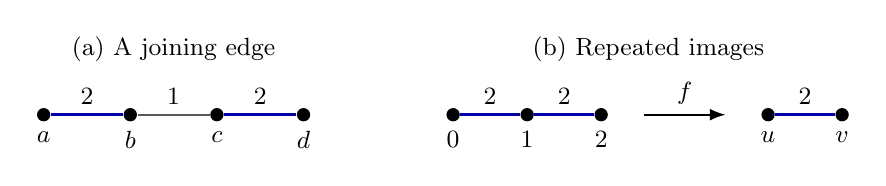
\begin{tikzpicture}[every node/.style={font=\small}]
\node at (1.65,0.83) {(a) A joining edge};
\node[graph vertex,label=below:$a$] (a) at (0,0) {};
\node[graph vertex,label=below:$b$] (b) at (1.1,0) {};
\node[graph vertex,label=below:$c$] (c) at (2.2,0) {};
\node[graph vertex,label=below:$d$] (d) at (3.3,0) {};
\draw[marked edge] (a)--node[above] {$2$} (b);
\draw[unmarked edge] (b)--node[above] {$1$} (c);
\draw[marked edge] (c)--node[above] {$2$} (d);

\begin{scope}[xshift=5.2cm]
\node at (2.48,0.83) {(b) Repeated images};
\node[graph vertex,label=below:$0$] (p0) at (0,0) {};
\node[graph vertex,label=below:$1$] (p1) at (0.94,0) {};
\node[graph vertex,label=below:$2$] (p2) at (1.88,0) {};
\node[graph vertex,label=below:$u$] (u) at (4,0) {};
\node[graph vertex,label=below:$v$] (v) at (4.94,0) {};
\draw[marked edge] (p0)--node[above] {$2$} (p1);
\draw[marked edge] (p1)--node[above] {$2$} (p2);
\draw[-{Latex[length=2mm]},semithick] (2.42,0)--node[above] {$f$} (3.46,0);
\draw[marked edge] (u)--node[above] {$2$} (v);
\end{scope}
\end{tikzpicture}
\caption{The edge $bc$ joins the marked edges in (a).
In (b), $f(0)=f(2)=u$ and $f(1)=v$.}
\label{fig:marked-maps}
\end{figure}

For the counts below, we use patterns whose underlying graph is
connected, whose edges of color $2$ form a strong clique in that
graph, and for which $c_F(0,1)=2$. We call $(0,1)$ the
\emph{ordered root}. For a fixed pattern $F$, let $h_F$ be the number
of maps $f\colon P_n\to V(G)$ for which
$c_G(f(i),f(j))=c_F(i,j)$ on every pair of distinct positions.

To express $h_F$ in terms of a probability, we sample a map
$f\colon P_n\to V(G)$. Begin with positions $0,1$ and set
$A_2=\{0,1\}$. For $i=2,\ldots,n-1$, choose an edge
$\{r_i,s_i\}$ of the underlying graph of $F$ with $r_i\in A_i$
and $s_i\in P_n\setminus A_i$, and set
$A_{i+1}=A_i\cup\{s_i\}$. Such an edge exists by connectedness.
We choose the images of $s_2,\ldots,s_{n-1}$ in this order after
choosing the images of $0,1$.

Choose $(f(0),f(1))$ uniformly from the $2m$ ordered marked edges of
$G$. At step $i$, choose $f(s_i)$ uniformly from the $\Delta$
neighbors of $f(r_i)$ in $G$, allowing repeated images. Each
sequence of choices determines a distinct map. Thus the
$2m\Delta^{n-2}$ resulting maps are equally likely.

For every map counted by $h_F$, the images of $0,1$ form an ordered
marked edge. Each $\{r_i,s_i\}$ has color $1$ or $2$ in $F$, so the
required $f(s_i)$ is among the neighbors of $f(r_i)$ available at
step $i$. Exactly $h_F$ of the resulting maps therefore satisfy
$c_G(f(r),f(s))=c_F(r,s)$ for all distinct $r,s\in P_n$. The
probability of obtaining $F$ is
\[
 q_F=\frac{h_F}{2m\Delta^{n-2}}.
\]

In \textbf{Subsection~\ref{subsec:marked-edge-pairs}}, we will express
$\frac{m}{\Delta^2}$ as a linear combination of the quantities $q_F$.
We now use the local flag algebra method to derive linear inequalities
in these quantities.

Fix a pattern $T$ on $P_k$, called the \emph{type}. A \emph{flag
of type $T$} is a pattern $F$ on $P_n$, with $n\geq k$, whose
colors satisfy
$c_F(r,s)=c_T(r,s)$ for all distinct $r,s\in P_k$.

In the simple-graph counts below, we choose the type and its flags
from the patterns used to define $q_F$. Their underlying graphs
are connected, their edges of color $2$ form strong cliques in
their respective underlying graphs, and their pair $\{0,1\}$ has
color $2$.

Fix a map $f\colon P_k\to V(G)$ that gives the colors of $T$.
A map $g\colon P_n\to V(G)$ is an \emph{extension of $f$ to $F$}
if it agrees with $f$ on $P_k$ and gives the colors of $F$ on every
pair of positions. Let $h_F(f)$ be the number of these extensions.

To express $h_F(f)$ in terms of a probability, we sample a map
$g\colon P_n\to V(G)$ with $g|_{P_k}=f$. Set $A_k=P_k$. For
$i=k,\ldots,n-1$, choose an edge $\{r_i,s_i\}$ of the underlying
graph of $F$ with $r_i\in A_i$ and $s_i\in P_n\setminus A_i$, and
set $A_{i+1}=A_i\cup\{s_i\}$. The underlying graph is connected,
so these edges exist.

Set $g|_{P_k}=f$. For $i=k,\ldots,n-1$ in order, choose $g(s_i)$
uniformly from the $\Delta$ neighbors of $g(r_i)$ in $G$, allowing
repeated images. This gives $\Delta^{n-k}$ equally likely maps.
Every extension counted by $h_F(f)$ occurs, since each pair
$\{r_i,s_i\}$ has color $1$ or $2$ in $F$ and its two images
are therefore adjacent. The probability of obtaining $F$ is
\[
 \frac{h_F(f)}{\Delta^{n-k}}.
\]
Take flags $F_i$ and $F_j$ of type $T$ on $n_i$ and $n_j$ positions,
respectively. Put
\[
 n=n_i+n_j-k,\qquad A=P_{n_i},\qquad B=P_k\cup\{n_i,\ldots,n-1\}.
\]
Keep the positions of $F_i$ in $A$. For $F_j$, let
$\rho\colon P_{n_j}\to B$ be given by
\begin{equation}\label{eq:flag-relabeling}
 \rho(r)=
 \begin{cases}
  r, & 0\leq r<k,\\
  n_i+r-k, & k\leq r<n_j.
 \end{cases}
\end{equation}
Give each pair $\{\rho(r),\rho(s)\}$ in $B$ the color $c_{F_j}(r,s)$.
The two position sets intersect in $P_k$, and their pair colors agree
there because both flags have type $T$. This construction also applies
when $i=j$.

Choose an extension $g_i$ of $f$ to $F_i$ on $A$ and an extension
$g_j$ of $f$ to $F_j$ on $B$. Both maps agree with $f$ on $P_k$,
so there is a unique map $g\colon P_n\to V(G)$ that equals $g_i$ on
$A$ and $g_j$ on $B$. Give each pair $\{r,s\}$ the color
$c_G(g(r),g(s))$. The color is $2$ if the images are joined by an
edge in $S$, $1$ if they are joined by another edge of $G$, and $0$
if they coincide or are nonadjacent. This defines a pattern $H$ on
$P_n$ whose colors on $A$ and $B$ are those of $F_i$ and $F_j$,
respectively.

Let $\{a,b\}$ and $\{c,d\}$ be disjoint pairs of color $2$ in $H$.
By the definition of $c_G$, the edges $g(a)g(b)$ and $g(c)g(d)$
belong to $S$. If their endpoint sets are disjoint, the strong
clique property of $S$ gives $r\in\{a,b\}$ and $s\in\{c,d\}$ with
$g(r)g(s)\in E(G)$. If their endpoint sets intersect, we may order
the positions within each pair so that $g(a)=g(c)$. Then
$g(a)g(d)=g(c)g(d)\in S$. In either case, a pair with one position
in $\{a,b\}$ and the other in $\{c,d\}$ has color $1$ or $2$. Thus
the edges of color $2$ form a strong clique in the underlying graph
of $H$.

Let $\mathcal U_{ij}$ be the set of patterns on $P_n$ obtained by
keeping the colors prescribed by $F_i$ on $A$ and by $F_j$ on $B$,
and allowing each of the colors $0,1,2$ on every pair $\{r,s\}$ with
$r\in A\setminus P_k$ and $s\in B\setminus P_k$. Retain an
assignment of these colors precisely when the edges of color $2$
form a strong clique in the resulting underlying graph. This graph
is connected because it contains the connected underlying graphs
on $A$ and $B$, which meet on $P_k$ and together cover $P_n$.

There are $h_{F_i}(f)$ choices for $g_i$ and $h_{F_j}(f)$ choices
for $g_j$. Each choice of $g_i$ and $g_j$ determines a unique map
$g$ and hence a unique pattern $H\in\mathcal U_{ij}$. Conversely,
every map $g$ counted by $h_H(f)$ arises from the unique choice
$(g|_A,g|_B)$, since $H$ has the colors prescribed by the two flags
on $A$ and $B$. Hence
\[
 h_{F_i}(f)h_{F_j}(f)=\sum_{H\in\mathcal U_{ij}}h_H(f).
\]

Fix a sequence $F_1,\ldots,F_s$ of flags of type $T$, with $n_i$
positions in $F_i$. For each map $f\colon P_k\to V(G)$ that gives the colors of
$T$, let $v(f)$ be the real column vector with entries
\[
 v_i(f)=\frac{h_{F_i}(f)}{\Delta^{n_i-k}}
 \qquad (1\leq i\leq s).
\]

Apply to $T$ the sampling rule for a connected pattern with ordered
root $(0,1)$. It gives $2m\Delta^{k-2}$ equally likely maps
$f\colon P_k\to V(G)$, including every map giving the colors of $T$.

Define the $s\times s$ matrix
\[
 M=\frac{1}{2m\Delta^{k-2}}\sum_f v(f)v(f)^{\mathsf T},
\]
where the sum runs over all maps $f\colon P_k\to V(G)$ that give the
colors of $T$. The factor $\frac{1}{2m\Delta^{k-2}}$ is the probability
of obtaining each such map in the sampling procedure. For every
real column vector $x\in\mathbb R^s$,
\[
 x^{\mathsf T}Mx
 =\frac{1}{2m\Delta^{k-2}}\sum_f\bigl(x^{\mathsf T}v(f)\bigr)^2
 \geq 0.
\]
Therefore $M$ is positive semidefinite.

Fix $i,j$ and put $n=n_i+n_j-k$, the number of positions in the
union of $F_i$ and $F_j$. The $(i,j)$ entry of $v(f)v(f)^{\mathsf T}$
is $v_i(f)v_j(f)$. Substituting the definitions of these two
components gives
\[
 M_{ij}
 =\frac{\displaystyle\sum_f h_{F_i}(f)h_{F_j}(f)}
        {2m\Delta^{k-2}\Delta^{n_i-k}\Delta^{n_j-k}}.
\]
The exponents of $\Delta$ in the denominator add to $n-2$.
For each $f$, the counting identity for $F_i$ and $F_j$ gives
\[
 h_{F_i}(f)h_{F_j}(f)=\sum_{H\in\mathcal U_{ij}}h_H(f).
\]

Fix $H\in\mathcal U_{ij}$. Since $H$ agrees with $T$ on $P_k$, each
map $g$ counted by $h_H$ is counted exactly once in $\sum_f h_H(f)$,
in the term with $f=g|_{P_k}$. Thus $\sum_f h_H(f)=h_H$, and
\[
 M_{ij}
 =\frac{\displaystyle\sum_{H\in\mathcal U_{ij}}h_H}
        {2m\Delta^{n-2}}
 =\sum_{H\in\mathcal U_{ij}}q_H,
\]
as in \eqref{eq:moment-expansion}. Since $M$ is positive
semidefinite, for every real column vector $x\in\mathbb R^s$,
\[
 \sum_{i,j=1}^{s}x_i x_j\sum_{H\in\mathcal U_{ij}}q_H
 =x^{\mathsf T}Mx\geq 0.
\]
For fixed $x$, this is a linear inequality in the $q_H$.
We call each such inequality a \emph{flag inequality}.
\textbf{Subsection~\ref{subsec:marked-edge-pairs}} uses these
inequalities to obtain an upper bound on $\frac{m}{\Delta^2}$.

\subsection{The Uniform Bound for Simple Graphs}\label{subsec:marked-edge-pairs}

We return to the $\Delta$-regular simple graph $G$ and the marked
strong clique $S$ of size $m>0$ from
\textbf{Subsection~\ref{subsec:adapted-flags}}. Let $\mathcal B$
consist of the patterns on $P_4$ whose underlying graphs are
connected, whose edges of color $2$ form a strong clique in the
underlying graph, and whose pairs $\{0,1\}$ and $\{2,3\}$ both
have color $2$.

Choose a first ordered marked edge $(u_0,u_1)$ and a second ordered
marked edge $(u_2,u_3)$. The two choices may use the same edge of
$S$. There are $(2m)^2$ choices in total. For each choice, define
$f\colon P_4\to V(G)$ by setting $f(r)=u_r$ for $r\in P_4$. The colors
$c_G(u_r,u_s)$ of the six position pairs determine a pattern $F$
on $P_4$, with color $2$ on both $\{0,1\}$ and $\{2,3\}$.

If the two chosen edges have disjoint endpoints, the strong clique
property of $S$ gives an edge of $G$ joining an endpoint of one to
an endpoint of the other. If they have a common endpoint, take
the position of that endpoint in the first pair and the position
of the other endpoint in the second pair. The pair of these two
positions has color $2$. In either case the underlying graph of
$F$ has an edge joining the two pairs of positions, so it is
connected. Applying the same argument to any two disjoint pairs
of color $2$ shows that the edges of color $2$ form a strong clique
in the underlying graph of $F$. Thus $F\in\mathcal B$, and this
map contributes one to $h_F$.

Conversely, fix $F\in\mathcal B$ and take any map $f$ counted by
$h_F$. Since $\{0,1\}$ and $\{2,3\}$ both have color $2$, the two
ordered marked edges are $(f(0),f(1))$ and $(f(2),f(3))$, in that
order. This gives a bijection between the ordered choices and the
maps counted by the $h_F$ for $F\in\mathcal B$. Therefore
\[
 \sum_{F\in\mathcal B}h_F=(2m)^2.
\]
Every $F\in\mathcal B$ has four positions, so
$q_F=\frac{h_F}{2m\Delta^2}$. It follows that
\[
 \frac{1}{2}\sum_{F\in\mathcal B}q_F
 =\frac{\displaystyle\sum_{F\in\mathcal B}h_F}{4m\Delta^2}
 =\frac{m}{\Delta^2}.
\]

Fix a pattern $F$ on $P_k$, where $k\geq 2$. Assume that its
underlying graph is connected, that the edges of color $2$ form a
strong clique in that graph, and that $c_F(0,1)=2$. Fix a position
$u\in P_k$. Let $\mathcal E(F,u)$ consist of the patterns $F'$
on $P_{k+1}$ that agree with $F$ on $P_k$, have color $1$ or $2$
on $\{u,k\}$, and whose edges of color $2$ form a strong clique
in the underlying graph. The underlying graph of each $F'$ is
connected because the new position $k$ is adjacent to $u$.

For each map $f$ counted by $h_F$, form a map
$g\colon P_{k+1}\to V(G)$ by keeping $g=f$ on $P_k$ and choosing
$g(k)$ from the $\Delta$ neighbors of $f(u)$. A vertex already used
by $f$ may be chosen again. The colors given by $g$ agree with $F$
on $P_k$ and give $\{u,k\}$ color $1$ or $2$. As for the patterns
on $P_4$, the edges of color $2$ form a strong clique in the
resulting underlying graph. Thus each choice gives a unique
pattern $F'\in\mathcal E(F,u)$. Conversely, each map counted by
$h_{F'}$ for $F'\in\mathcal E(F,u)$ determines its restriction to
$P_k$ and the chosen neighbor at position $k$. Hence
\[
 \sum_{F'\in\mathcal E(F,u)}h_{F'}=\Delta h_F.
\]
Dividing by $2m\Delta^{k-1}$ gives the degree equation
\[
 \sum_{F'\in\mathcal E(F,u)}q_{F'}=q_F,
\]
as in \eqref{eq:degree-extension}.

\textbf{Subsection~\ref{sec:simple-proof}} uses the degree equations
to express
\[
 \frac{5}{4}-\frac{1}{2}\sum_{F\in\mathcal B}q_F
\]
as a sum of nonnegative multiples of the $q_F$ and of the quadratic
forms $x^{\mathsf T}Mx$ from
\textbf{Subsection~\ref{subsec:adapted-flags}}. Since each $q_F$ is
nonnegative and each matrix $M$ is positive semidefinite, the
difference is nonnegative. Thus
\[
 \frac{m}{\Delta^2}=\frac{1}{2}\sum_{F\in\mathcal B}q_F
 \leq\frac{5}{4},
\]
so $m\leq\frac{5}{4}\Delta^2$.

\subsection{The Weighted Flag Algebra Method}\label{subsec:weighted-sketch}

Let $D$ be a positive integer and let $G$ be a loopless multigraph
of maximum degree at most $D$. Fix a strong clique of $m>0$ edges
and mark its edges. We first reduce $G$ by deleting every vertex
that is not an endpoint of a marked edge, together with its incident
edges. Then, for each adjacent pair $u,v$ in the resulting multigraph,
do the following. If at least one edge with endpoints $u,v$ is
marked, delete all unmarked edges with those endpoints. If all edges
with endpoints $u,v$ are unmarked, keep one of them and delete the
rest. This reduction preserves every marked edge and every adjacency
between endpoints of marked edges. Hence the marked edges still form
a strong clique.

We then embed the reduced multigraph as an induced subgraph of a
$D$-regular loopless multigraph. Every added edge is unmarked and
has multiplicity one, so the marked edges and their multiplicities
are preserved. The construction is given in
\textbf{Lemma~\ref{lem:regularization}}.

Write $G$ for the completed multigraph and let $G_{\rm s}$ be its
underlying simple graph. Color an edge $uv$ of $G_{\rm s}$ red if there is a marked
edge with endpoints $u,v$ in the multigraph, and blue otherwise.
For each red edge $uv$, choose one such marked edge as its
representative. Let $b_{uv}$ be the number of remaining marked edges
with those endpoints. If $G_{\rm s}$ has $s$ red edges, then exactly
$s$ marked edges are chosen as representatives, leaving $b=m-s$
other marked edges.

We now define a \emph{weighted pattern} on $P_n$ to be a pair $(F,J)$,
where $F$ is a pattern and $J$ is a set of pairs of color $2$ in
$F$ such that the graph with vertex set $P_n$ and edge set $J$ is a
forest. We call the elements of $J$ the \emph{specified pairs}.

A map $\phi\colon P_n\to V(G_{\rm s})$ gives a position pair color
$2$ if its images are joined by a red edge, color $1$ if they are
joined by a blue edge, and color $0$ if they coincide or are
nonadjacent. For a weighted pattern $(F,J)$, define
\[
 Q(F,J)=\frac{1}{2mD^{n-2}}\sum_\phi
        \prod_{\{r,t\}\in J} b_{\phi(r)\phi(t)},
\]
where the sum runs over all maps $\phi$ that give the colors of $F$
on every position pair. When $J=\varnothing$, the product is $1$.
If $h$ specified pairs have the same image $\{u,v\}$, their factors
in the product give $b_{uv}^{h}$.

In \textbf{Subsection~\ref{subsec:weighted-uniform-sketch}}, we will
express $\frac{m}{D^2}$ as a linear combination of the quantities
$Q(F,J)$. We now use our weighted flag algebra method to derive
linear inequalities in these quantities.

A \emph{weighted type} is a weighted pattern $(T,J_0)$ in which
$T$ is a type on $P_k$. A \emph{weighted flag of type $(T,J_0)$}
is a weighted pattern $(F,J)$ in which $F$ is a flag of type $T$
and the specified pairs of $J$ contained in $P_k$ are exactly
those in $J_0$.

Fix a sequence of weighted flags $(F_1,J_1),\ldots,(F_\ell,J_\ell)$
of type $(T,J_0)$, where $(F_i,J_i)$ is on $P_{n_i}$. For each map
$\phi\colon P_k\to V(G_{\rm s})$ that gives the colors of $T$, define
\[
 w(\phi)=\prod_{\{r,t\}\in J_0} b_{\phi(r)\phi(t)}.
\]
This product counts the ways to choose one remaining marked edge
with endpoints $\phi(r),\phi(t)$ for each pair $\{r,t\}\in J_0$.

For each $i$, consider all maps $g\colon P_{n_i}\to V(G_{\rm s})$
such that $g|_{P_k}=\phi$ and $g$ gives the colors of $F_i$ on each
position pair. Define
\[
 a_i(\phi)=\sum_g\prod_{\{r,t\}\in J_i\setminus J_0} b_{g(r)g(t)},
\]
where the sum runs over these maps. For a fixed $g$, the product counts
the ways to choose one remaining marked edge with endpoints $g(r),g(t)$
for each specified pair $\{r,t\}$ with at least one position outside
$P_k$. In both products, the choice is made separately for each pair.

Let $v(\phi)$ be the column vector with entries
$v_i(\phi)=\frac{a_i(\phi)}{D^{n_i-k}}$. The \emph{weighted matrix}
of this sequence is
\[
 W=\frac{1}{2mD^{k-2}}\sum_\phi w(\phi)v(\phi)v(\phi)^{\mathsf T},
\]
where the sum runs over all maps $\phi\colon P_k\to V(G_{\rm s})$
that give the colors of $T$. For every $x\in\mathbb R^\ell$,
\[
 x^{\mathsf T}Wx=\frac{1}{2mD^{k-2}}\sum_\phi
 w(\phi)\bigl(x^{\mathsf T}v(\phi)\bigr)^2\geq0,
\]
since each $w(\phi)$ is nonnegative. Thus $W$ is positive
semidefinite.

Fix $i,j$ and put $n=n_i+n_j-k$. Keep $F_i$ on $A=P_{n_i}$ and
use the map $\rho$ in \eqref{eq:flag-relabeling} to relabel $F_j$
on $B=P_k\cup\{n_i,\ldots,n-1\}$. Write
\[
 J_j^B=\bigl\{\{\rho(r),\rho(t)\}\mid\{r,t\}\in J_j\bigr\},
 \qquad J_{ij}=J_i\cup J_j^B.
\]
Since $A\cap B=P_k$ and both weighted flags have type $(T,J_0)$,
we have $J_i\cap J_j^B=J_0$. Thus $J_{ij}$ is the disjoint union of
$J_0$, $J_i\setminus J_0$, and $J_j^B\setminus J_0$.

Fix a map $\phi$ giving the colors of $T$. Let $g_i$ and $g_j$ range
over the extensions of $\phi$ to $F_i$ on $A$ and to the relabeled
$F_j$ on $B$, respectively. For each pair
$(g_i,g_j)$, let $g\colon P_n\to V(G_{\rm s})$ be the map with
$g|_A=g_i$ and $g|_B=g_j$. In particular, $g|_{P_k}=\phi$.
Substituting the definitions of $w(\phi)$, $a_i(\phi)$, and
$a_j(\phi)$ gives
\[
\begin{aligned}
 w(\phi)a_i(\phi)a_j(\phi)
 &=\sum_{g_i,g_j}
  \left(\prod_{\{r,t\}\in J_0} b_{\phi(r)\phi(t)}\right)
  \left(\prod_{\{r,t\}\in J_i\setminus J_0} b_{g_i(r)g_i(t)}\right)
  \left(\prod_{\{r,t\}\in J_j^B\setminus J_0} b_{g_j(r)g_j(t)}\right)\\
 &=\sum_{g_i,g_j}\prod_{\{r,t\}\in J_{ij}} b_{g(r)g(t)}.
\end{aligned}
\]
The second equality holds because $J_0$, $J_i\setminus J_0$, and
$J_j^B\setminus J_0$ partition $J_{ij}$, and the map used in each
product agrees with $g$ on the positions in that product.

Let $\mathcal U_{ij}$ consist of the patterns $H$ on $P_n$ obtained
by keeping the colors prescribed by $F_i$ on $A$ and by the relabeled
$F_j$ on $B$. For each pair $\{r,t\}$ with $r\in A\setminus P_k$
and $t\in B\setminus P_k$, allow any of the colors $0,1,2$.
Retain a pattern if its edges of color $2$ form a strong clique
in its underlying graph. The colors prescribed on $A$ and $B$
give color $2$ to every pair in $J_{ij}$. Thus, if $J_{ij}$ is a
forest, $(H,J_{ij})$ is a weighted pattern for each
$H\in\mathcal U_{ij}$.

Note that $J_{ij}$ need not be a forest. For example, take the
common type on $\{0,1\}$ with its pair of color $2$ and with
$J_0=\varnothing$. Take $F_i$ and $F_j$ to be triangles whose edges
all have color $2$. After relabeling, their third positions are
$2$ and $3$, respectively. Set
\[
 J_i=\bigl\{\{0,2\},\{1,2\}\bigr\},
 \qquad J_j^B=\bigl\{\{0,3\},\{1,3\}\bigr\}.
\]
Each specified set forms a path. Their union $J_{ij}$ forms the
cycle $0,2,1,3,0$.

The combined map $g$ gives the prescribed colors on $A$ and $B$
and determines the colors of all remaining pairs. Let $H$ be the
resulting pattern, and take two disjoint pairs $\{a,b\}$ and
$\{c,d\}$ of color $2$ in $H$. The multigraph has a marked edge
with endpoints $g(a),g(b)$ and a marked edge with endpoints
$g(c),g(d)$. If these endpoint sets are disjoint, the strong clique
of marked edges guarantees a multigraph edge joining a vertex of the
first set to a vertex of the second. These vertices are adjacent in
$G_{\rm s}$, which has an edge for every adjacent pair of vertices
in the multigraph. Hence the corresponding position pair has color
$1$ or $2$. If the endpoint sets meet, order the positions within
each pair so that $g(a)=g(c)$. Then $g(a)g(d)=g(c)g(d)$ is a red
edge of $G_{\rm s}$, so $\{a,d\}$ has color $2$. In either case, an
edge of the underlying graph of $H$ joins the two pairs. Thus,
for any pattern $H$ given by a map into $G_{\rm s}$ and any two
disjoint pairs $\{a,b\}$ and $\{c,d\}$ of color $2$ in $H$,
\begin{equation}\label{eq:weighted-joining-edge}
 \max_{r\in\{a,b\},\,t\in\{c,d\}} c_H(r,t)\geq 1.
\end{equation}
In particular, the edges of color $2$ in the pattern given by the
combined map $g$ form a strong clique in its underlying graph, so
$H\in\mathcal U_{ij}$.

Conversely, fix $H\in\mathcal U_{ij}$ and a map
$g\colon P_n\to V(G_{\rm s})$ giving its colors. Since $H$ agrees
with $F_i$ on $A$ and with the relabeled $F_j$ on $B$, set
\[
 \phi=g|_{P_k},\qquad g_i=g|_A,\qquad g_j=g|_B.
\]
The map $\phi$ gives the colors of $T$, and $g_i$ and $g_j$ are its
extensions to the two flags. These restrictions are determined
uniquely by $g$, and combining $g_i$ and $g_j$ gives $g$.
Thus when we sum the identity over $\phi$, each map $g$ giving the
colors of some $H\in\mathcal U_{ij}$ occurs once. Grouping by $H$ gives
\[
\begin{aligned}
 \sum_\phi w(\phi)a_i(\phi)a_j(\phi)
 &=\sum_\phi\sum_{g_i,g_j}
  \prod_{\{r,t\}\in J_{ij}} b_{g(r)g(t)}\\
 &=\sum_{H\in\mathcal U_{ij}}
  \sum_{g\text{ giving the colors of }H}
  \prod_{\{r,t\}\in J_{ij}} b_{g(r)g(t)}.
\end{aligned}
\]

Substituting $v_i(\phi)$ and $v_j(\phi)$ into the definition of $W$
gives the denominator $2mD^{n-2}$ in $W_{ij}$, since the exponent
on $D$ is $(k-2)+(n_i-k)+(n_j-k)=n-2$.
If $J_{ij}$ is a forest, we can use the grouped sum above to write
\[
\begin{aligned}
 W_{ij}
 &=\frac{\displaystyle\sum_\phi w(\phi)a_i(\phi)a_j(\phi)}
         {2mD^{n-2}}\\
 &=\sum_{H\in\mathcal U_{ij}}\frac{1}{2mD^{n-2}}
  \sum_{g\text{ giving the colors of }H}
  \prod_{\{r,t\}\in J_{ij}} b_{g(r)g(t)}\\
 &=\sum_{H\in\mathcal U_{ij}} Q(H,J_{ij}).
\end{aligned}
\]
The last equality follows from the definition of $Q$.
When this formula applies to every entry of $W$, the inequality
$x^{\mathsf T}Wx\geq0$ gives a linear inequality in the quantities
$Q(H,J_{ij})$ for each fixed $x\in\mathbb R^\ell$. We call each
such inequality a \emph{weighted flag inequality}.

\subsection{The Uniform Bound for Loopless Multigraphs}
\label{subsec:weighted-uniform-sketch}

Let $G$ denote the $D$-regular loopless multigraph constructed in
\textbf{Subsection~\ref{subsec:weighted-sketch}} to contain the
reduced multigraph as an induced subgraph, and let $G_{\rm s}$
denote its underlying simple graph. Let $m$ be the number of marked
edges of $G$, $s$ the number of red edges of $G_{\rm s}$, and
$b=m-s$ the number of remaining marked edges after one
representative has been chosen for each red edge. Put
\[
 M=\frac{m}{D^2},\qquad S=\frac{s}{D^2},\qquad e=\frac{b}{m}.
\]
Then $S=M(1-e)$. The red edges form a strong clique in $G_{\rm s}$,
and $\Delta(G_{\rm s})\leq D$, so the simple-graph bound in
\textbf{Subsection~\ref{subsec:marked-edge-pairs}} gives
$S\leq\frac{5}{4}$.

Put $R=\{\{0,1\},\{2,3\}\}$. Let $\mathcal B$ be the set of patterns
$F$ on $P_4$ with $c_F(0,1)=c_F(2,3)=2$, whose underlying graph is
connected and whose edges of color $2$ form a strong clique in that
graph.

Choose marked edges $\varepsilon_1,\varepsilon_2$ with ordered
endpoints $(u_0,u_1)$ and $(u_2,u_3)$, respectively, allowing
$\varepsilon_1=\varepsilon_2$. Set $\phi(r)=u_r$ for $r\in P_4$.
The pattern $F$ given by $\phi$ has color $2$ on both pairs in $R$.
By \eqref{eq:weighted-joining-edge}, its edges of color $2$ form a
strong clique, and an edge joins the two pairs in $R$. Thus the
underlying graph is connected and $F\in\mathcal B$.

Fix $F\in\mathcal B$, a map $\phi$ giving the colors of $F$, and a
set $J\subseteq R$. We count choices of the marked edges
$\varepsilon_1,\varepsilon_2$ with ordered endpoints
$(\phi(0),\phi(1))$ and $(\phi(2),\phi(3))$, respectively. For each
position pair $\{r,t\}\in R$, require the selected edge to be a
remaining marked edge if $\{r,t\}\in J$, and the representative if
$\{r,t\}\in R\setminus J$. There are $b_{\phi(r)\phi(t)}$ choices
for each pair in $J$ and one choice for each pair in $R\setminus J$.
Thus the number of choices of $(\varepsilon_1,\varepsilon_2)$
satisfying these requirements is
\[
 \prod_{\{r,t\}\in J} b_{\phi(r)\phi(t)}.
\]
Since the two pairs in $R$ are disjoint, every $J\subseteq R$ is a
forest, so $(F,J)$ is a weighted pattern. Summing the product over
the maps $\phi$ giving the colors of $F$ gives $2mD^2Q(F,J)$.

Each ordered choice of two marked edges determines $\phi$ and
hence $F$, as well as the set $J$ of pairs on which a remaining
marked edge was chosen. Thus summing over $F$ and $J$ counts each
ordered choice exactly once. The strong clique has $m$ marked
edges, each with two endpoint orders, so there are $(2m)^2$
choices in total. Hence
\[
 2mD^2\sum_{F\in\mathcal B}\sum_{J\subseteq R} Q(F,J)=(2m)^2.
\]
Dividing by $4mD^2$ gives
\[
 M=\frac{m}{D^2}=\frac{1}{2}
   \sum_{F\in\mathcal B}\sum_{J\subseteq R}Q(F,J).
\]

For a weighted pattern $(H,K)$ on $P_\ell$, let $h(H,K)$ count
the tuples $\bigl(g,(\eta_q)_{q\in K}\bigr)$, where
$g\colon P_\ell\to V(G_{\rm s})$ gives the colors of $H$, and
$\eta_q$ is a remaining marked edge with endpoints $g(r),g(t)$
for each $q=\{r,t\}\in K$. For fixed $g$, the edge on each pair
is chosen separately in $b_{g(r)g(t)}$ ways. Summing over $g$ gives
\[
 h(H,K)=\sum_{g\text{ giving the colors of }H}
  \prod_{\{r,t\}\in K} b_{g(r)g(t)}=2mD^{\ell-2}Q(H,K).
\]

We now derive the degree equation for a weighted pattern $(F,J)$.
Let $(F,J)$ be on $P_k$, with a connected underlying graph in
which the edges of color $2$ form a nonempty strong clique.
Fix $u\in P_k$ and put $p=\{u,k\}$. For $c\in\{1,2\}$,
let $\mathcal E_c(F,u)$ consist of the patterns $H$ on $P_{k+1}$
that agree with $F$ on $P_k$, satisfy $c_H(u,k)=c$, and whose edges
of color $2$ form a strong clique in the underlying graph. The
underlying graph of each $H$ is connected because the new
position $k$ is adjacent to $u$.

An extension of $(F,J)$ at $u$ consists of a tuple
$\bigl(\phi,(\eta_q)_{q\in J}\bigr)$ counted by $h(F,J)$ and a choice
of an edge $\varepsilon$ of $G$ incident with $\phi(u)$. For each
tuple there are exactly $D$ choices of $\varepsilon$, counting
parallel edges separately. Thus there are $D\,h(F,J)$ extensions
of $(F,J)$ at $u$.

For each extension, define $g$ by $g|_{P_k}=\phi$ and let $g(k)$
be the other endpoint of $\varepsilon$. The pattern $H$ given by
$g$ agrees with $F$ on $P_k$ and has $c=c_H(u,k)\in\{1,2\}$,
since $g(u)$ and $g(k)$ are joined by $\varepsilon$.
By \eqref{eq:weighted-joining-edge}, $H\in\mathcal E_c(F,u)$.
Keep the selected edges $(\eta_q)_{q\in J}$ and determine the new
specified set $J'$ as follows.
\[
 (c,J')=
 \begin{cases}
  (1,J), & \varepsilon\text{ is unmarked},\\
  (2,J), & \varepsilon\text{ is a representative},\\
  (2,J\cup\{p\}), & \varepsilon\text{ is a remaining marked edge}.
 \end{cases}
\]
In the third case record $\eta_p=\varepsilon$. Adding $p$ preserves
the forest condition because $k$ is a new position. This gives a
tuple $\bigl(g,(\eta_q)_{q\in J'}\bigr)$ counted by $h(H,J')$.

Conversely, fix $H\in\mathcal E_c(F,u)$ and a set $J'$ allowed
for this value of $c$ in the three cases above. Given a tuple
$\bigl(g,(\eta_q)_{q\in J'}\bigr)$ counted by $h(H,J')$, set
$\phi=g|_{P_k}$ and retain $(\eta_q)_{q\in J}$. Define
$\varepsilon$ by
\[
 \varepsilon=
 \begin{cases}
  \text{the unique unmarked edge with endpoints $g(u),g(k)$},
       &(c,J')=(1,J),\\
  \text{the representative with endpoints $g(u),g(k)$},
       &(c,J')=(2,J),\\
  \eta_p,&(c,J')=(2,J\cup\{p\}).
 \end{cases}
\]
The unique unmarked edge in the first case exists because the
reduction retains one edge on each unmarked pair and each edge
added in the completion is single. In each case $\varepsilon$ is
incident with $\phi(u)$ and extending along it gives the original
tuple. Thus $h(H,J')$ counts exactly the extensions that yield $H$
and $J'$. Summing over $H$ and the allowed sets $J'$ gives
\[
 \sum_{H\in\mathcal E_1(F,u)}h(H,J)
 +\sum_{H\in\mathcal E_2(F,u)}
  \bigl(h(H,J)+h(H,J\cup\{p\})\bigr)=D\,h(F,J).
\]
Each $H$ has $k+1$ positions, while $F$ has $k$ positions.
Dividing by $2mD^{k-1}$ and using the relation between $h$ and
$Q$ gives the degree equation
\[
 \sum_{H\in\mathcal E_1(F,u)}Q(H,J)
 +\sum_{H\in\mathcal E_2(F,u)}
  \bigl(Q(H,J)+Q(H,J\cup\{p\})\bigr)=Q(F,J).
\]

Suppose that $M>\frac{5}{4}$. The certificates in
\textbf{Appendix~\ref{app:weighted-final-checks}} use the degree
equations and weighted flag inequalities to give
$M<1.28492$ and $e<\frac{421}{2000}$.
Take an interval $[M_-,M_+]$ from
\textbf{Table~\ref{tab:uniform-chain}} in
\textbf{Subsection~\ref{sec:weighted-counts}} and suppose that
$M_-\leq M\leq M_+$. For the value $\alpha$ in that row, the
degree estimates give $\frac{R(C)}{D}\geq\alpha$ for every induced
red five-cycle $C$, where $R(C)$ is the sum of the five
remaining-degree bounds in \eqref{eq:odd-core-defs}.

Summing over the cycles and dividing by $2sD^3$ gives
$L_R\geq\alpha q_C$, where $L_R$ is the normalized sum of
$\frac{R(C)}{D}$ and $q_C$ is the normalized number of cycles,
counted with a starting vertex and direction. Both quantities
are zero when there are no such cycles. Using this inequality in
the simple-graph flag inequalities \eqref{eq:support-projection-four}
gives an upper bound $S\leq S_+$ for the interval. Since
$S=M(1-e)$ and $M\geq M_-$,
\[
 e=1-\frac{S}{M}
 \geq 1-\frac{S_+}{M}
 \geq 1-\frac{S_+}{M_-}.
\]

With this lower bound and $e<\frac{421}{2000}$, the six-position
weighted certificates in \textbf{Subsection~\ref{sec:weighted-counts}}
give $M<M_-$, contradicting $M\in[M_-,M_+]$. Starting from
$M<1.28492$, the first four rows of
\textbf{Table~\ref{tab:uniform-chain}} successively give $M<1.283$,
$M<1.279$, $M<1.274$, and $M<1.268$. The last row rules out the
remaining range $\frac{5}{4}<M<1.268$. Thus $m\leq\frac{5}{4}D^2$.
For even $D$, the right-hand side is $f(D)$.

\section{Auxiliary Lemmas}\label{sec:auxiliary}

We use a regular supergraph to count the ways to extend a map by one
vertex. We extend the regularization lemma of Davey et
al.~\cite{DaveyEtAlStrong2026} from simple graphs to
loopless multigraphs. The construction preserves the multiplicities
of the original edges and gives every new edge multiplicity one.

\begin{lemma}\label{lem:regularization}
Let $D\geq1$ be an integer and let $G$ be a finite loopless multigraph
with $\Delta(G)\leq D$. There is a finite $D$-regular loopless multigraph
$\widehat G$ containing $G$ as an induced subgraph such that every
edge of $\widehat G$ outside $G$ has multiplicity one. In particular, $\widehat G$ is simple
if $G$ is simple.
\end{lemma}

\begin{proof}
The sum of the degree deficits in $G$ is
\[
 \sum_{v\in V(G)}\bigl(D-d_G(v)\bigr)=D|V(G)|-2|E(G)|.
\]
If the sum is even, set $G_0=G$. If it is odd, then $D$ is odd.
Adjoin one isolated vertex to form $G_0$. The sum increases by $D$
and is therefore even in $G_0$.

Index the edges to be added at vertices of $G_0$ by
\[
 \mathcal I=\bigl\{(v,i):v\in V(G_0),\ i\in\mathbb Z,\
                   1\leq i\leq D-d_{G_0}(v)\bigr\}.
\]
Since $|\mathcal I|$ is even, choose a partition $\mathcal P$ of
$\mathcal I$ into two-element sets. For each
$P=\{(u,i),(v,j)\}\in\mathcal P$, add a copy of $K_{D+1}$ on new
vertices. Choose distinct vertices $x_P,y_P$ in this copy, delete
$x_Py_P$, and add $ux_P$ and $vy_P$. Write $\widehat G$ for the
resulting graph.

Each index $(v,i)$ contributes one edge at $v$, so
$d_{\widehat G}(v)=d_{G_0}(v)+|\{i:(v,i)\in\mathcal I\}|=D$
for $v\in V(G_0)$. Deleting $x_Py_P$ reduces the degrees of
$x_P$ and $y_P$ to $D-1$, and the edges to $G_0$ increase
both to $D$. The other vertices of each copy of $K_{D+1}$
have degree $D$ throughout. Thus $\widehat G$ is $D$-regular.
All added edges have at least one new endpoint and multiplicity
one. Hence $\widehat G$ is loopless and $\widehat G[V(G)]=G$.
\end{proof}

A strong clique in $G$ is also a strong clique in $\widehat G$, since
every adjacency between endpoints of its edges is preserved. In the
counting arguments we mark only the edges of the chosen clique, so
all edges added in the construction are unmarked.

Vector inequalities are coordinatewise. For symmetric matrices $X$
and $Y$ of the same size, $\tr(XY)=\sum_{i,j}X_{ij}Y_{ij}$.

In the simple-graph calculation we will express the size of a strong
clique, divided by the square of the maximum degree, as a linear
function of the pattern counts. The calculation uses a system with $N=23{,}789$ coordinates, $3{,}516$ linear equations and
$57$ positive semidefinite matrix constraints. Write $Aq=b$ for the
linear equations and $o^{\mathsf T}q$ for the objective, where
$A\in\mathbb Q^{3516\times N}$, $b\in\mathbb Q^{3516}$ and
$o\in\mathbb Q^N$. For each $\ell\in[57]$, let
$K_\ell,D_{\ell1},\ldots,D_{\ell N}$ be symmetric rational matrices of
the same size. The $\ell$th matrix constraint is $M_\ell(q)\succeq0$,
where
\begin{equation}\label{eq:intro-affine-gram}
 M_\ell(q)=K_\ell+\sum_{j=1}^N q_jD_{\ell j}.
\end{equation}
The matrices and vectors are specified in \textbf{Appendix~\ref{app:data-specification}}.
For a symmetric matrix
$Q$ of the same size as $K_\ell$, define
$D_\ell^*(Q)\in\mathbb R^N$ by
\begin{equation}\label{eq:intro-trace-adjoint}
 (D_\ell^*(Q))_j=\tr(QD_{\ell j})\qquad(j\in[N]).
\end{equation}

\begin{lemma}\label{prop:certificate-principle}
Let $o\in\mathbb Q^N$ be an objective vector and
$\lambda\in\mathbb Q^{3516}$. For each $\ell\in[57]$, let $Q_\ell$
be a matrix of the same size as $K_\ell$ expressible as a finite
nonnegative rational linear combination of outer products
$ww^{\mathsf T}$ of rational vectors. Set
\begin{align}
 &r=A^{\mathsf T}\lambda-\sum_{\ell=1}^{57}D_\ell^*(Q_\ell)-o,
 \label{eq:residual}\\
 &C=b^{\mathsf T}\lambda+\sum_{\ell=1}^{57}\tr(Q_\ell K_\ell).
 \label{eq:dual-value}
\end{align}
We call $r$ the residual vector. If $r\geq0$, then every $q\in\mathbb R^N$ with $q\geq0$, $Aq=b$ and
$M_\ell(q)\succeq0$ for all $\ell\in[57]$ satisfies $o^{\mathsf T}q\leq C$.
If $q\in[0,1]^N$ satisfies the same equations and matrix constraints,
then $o^{\mathsf T}q\leq C-\sum_{j:r_j<0}r_j$, for any residual $r$.
\end{lemma}

\begin{proof}
Fix $q\geq0$ with $Aq=b$ and $M_\ell(q)\succeq0$ for
$\ell\in[57]$. To bound $o^{\mathsf T}q$, express $C-o^{\mathsf T}q$
using the residual and matrix terms. Take the scalar product of
the identity for $r$ in \eqref{eq:residual} with $q$. Since $Aq=b$,
\[
 r^{\mathsf T}q=b^{\mathsf T}\lambda-o^{\mathsf T}q
       -\sum_{\ell=1}^{57}D_\ell^*(Q_\ell)^{\mathsf T}q.
\]
By \eqref{eq:intro-affine-gram} and \eqref{eq:intro-trace-adjoint},
$D_\ell^*(Q_\ell)^{\mathsf T}q
=\tr(Q_\ell M_\ell(q))-\tr(Q_\ell K_\ell)$.
Substitution and \eqref{eq:dual-value} give
\begin{equation}\label{eq:certificate-identity}
 C-o^{\mathsf T}q
 =\sum_{\ell=1}^{57}\tr\bigl(Q_\ell M_\ell(q)\bigr)
  +\sum_{j=1}^N r_jq_j.
\end{equation}
For each $\ell$, write
$Q_\ell=\sum_a\alpha_{\ell a}w_{\ell a}w_{\ell a}^{\mathsf T}$,
where each $\alpha_{\ell a}$ is nonnegative. Since
$M_\ell(q)\succeq0$,
\[
 \tr\bigl(Q_\ell M_\ell(q)\bigr)=
 \sum_a\alpha_{\ell a}w_{\ell a}^{\mathsf T}M_\ell(q)w_{\ell a}\geq0
\]
If $r\geq0$, the second sum in \eqref{eq:certificate-identity}
is also nonnegative, so $o^{\mathsf T}q\leq C$.
For $0\leq q_j\leq1$, we have $r_jq_j\geq0$ if $r_j\geq0$ and
$r_jq_j\geq r_j$ if $r_j<0$. Thus \eqref{eq:certificate-identity}
gives $o^{\mathsf T}q\leq C-\sum_{j:r_j<0}r_j$.
\end{proof}
\relax\space% End source/auxiliary.tex
% Begin source/proof_uniform.tex
\section{The Proof of the Bound \texorpdfstring{$\frac{5}{4}\Delta^2$}{5 Delta squared / 4}}\label{sec:uniform}

Let $G$ be a finite loopless multigraph with maximum degree $\Delta$.
We prove that $\omega(L(G)^2)\leq\frac{5}{4}\Delta^2$. We first
prove the bound for simple graphs. To extend it to multigraphs, we
count how many edges of a given strong clique join each pair of
adjacent vertices.

\subsection{The Bound \texorpdfstring{$\frac{5}{4}\Delta^2$}{5 Delta squared / 4} in Simple Graphs}
\label{sec:simple-proof}\label{sec:finite-model}\label{sec:identities}\label{sec:finite-instance}
\label{subsubsec:conditional-extension-counts}

By \textbf{Lemma~\ref{lem:regularization}}, a nonempty strong clique
in a simple graph of maximum degree $\Delta$ remains a strong clique
in a $\Delta$-regular simple graph. Let $G$ be this regular graph and
mark the set $S$ of edges in the given clique. We retain the other
edges of $G$, which may join the endpoints of disjoint marked edges.
The symmetric function
$c_G\colon V(G)\times V(G)\to\{0,1,2\}$ is given by
\[
 c_G(u,v)=
 \begin{cases}
  2,&uv\in S,\\
  1,&uv\in E(G)\setminus S,\\
  0,&u=v\text{ or }uv\notin E(G).
 \end{cases}
\]

\begin{defn}\label{def:patterns}
For an integer $n\geq2$, put $P_n=\{0,\ldots,n-1\}$. A \emph{pattern}
$F$ of order $n$ assigns a color $c_F(i,j)\in\{0,1,2\}$ to each pair
$ij=\{i,j\}$ of distinct positions in $P_n$, with $c_F(0,1)=2$. We
call $(0,1)$ the ordered root. The underlying graph $H$ of $F$ has
vertex set $P_n$ and edge set consisting of the pairs of color $1$
or $2$. We call $F$ \emph{connected} if $H$ is connected and
\emph{admissible} if the pairs of color $2$ form a clique in $L(H)^2$.
Equivalently, for every two disjoint pairs of color $2$, some pair
with one position in each has color $1$ or $2$.
Let $\mathcal F_n$ be the set of connected admissible patterns of order $n$.
\end{defn}

\begin{defn}\label{def:color-preserving-maps}
Let $F$ be a pattern of order $n$, and let $G$ be a finite simple graph
with marked set $S\subseteq E(G)$. A \emph{color-preserving map} from $F$
to $G$ is a map $f\colon P_n\to V(G)$ such that
$c_F(i,j)=c_G(f(i),f(j))$ for all distinct $i,j\in P_n$.
For fixed $G$ and $S$, let $h_F$ be the number of color-preserving maps
from $F$ to $G$.
\end{defn}

Distinct positions may map to the same vertex, in which case their
pair has color $0$.

\begin{lemma}\label{lem:pullback}
Let $G$ be a finite simple graph, let $S\subseteq E(G)$ be a clique
in $L(G)^2$, and let $n\geq 2$. Every map $f\colon P_n\to V(G)$ with
$c_G(f(0),f(1))=2$ gives an admissible pattern $F$ by setting
$c_F(i,j)=c_G(f(i),f(j))$ for all distinct $i,j\in P_n$.
\end{lemma}

\begin{proof}
To verify admissibility, take disjoint pairs $ij$ and $k\ell$ of
color $2$ in $F$. Their images $f(i)f(j)$ and $f(k)f(\ell)$ are
edges of $S$. If these edges are disjoint, the strong clique
property gives $r\in\{i,j\}$ and $s\in\{k,\ell\}$ for which
$f(r)f(s)\in E(G)$. The pair $rs$ has color $1$ or $2$.
If the two image edges have a common endpoint, name the positions
so that $f(i)=f(k)$. Then $f(j)f(k)=f(j)f(i)\in S$, so $jk$
has color $2$. In each case there is an edge of the underlying
graph of $F$ joining the two pairs of positions.
\end{proof}

Let $G$ be a finite simple $\Delta$-regular graph with $\Delta>0$,
and let $S\subseteq E(G)$ be a nonempty clique in $L(G)^2$ of size $m$.
For $F\in\mathcal F_n$, define
\begin{equation}\label{eq:q-definition}
 q_F=\frac{h_F}{2m\Delta^{n-2}}.
\end{equation}
The factor $2m$ counts the possible images of the ordered root.
For the two-position pattern $E_\star$ with its unique pair marked,
we have $h_{E_\star}=2m$ and hence $q_{E_\star}=1$.

Two patterns $F,F'\in\mathcal F_n$ are equivalent if there is a
permutation $\pi$ of $P_n$ with
$c_F(i,j)=c_{F'}(\pi(i),\pi(j))$ for every pair $ij$ of distinct
positions. The preimage of $\{0,1\}$ under $\pi$ may be any pair of
color $2$ in $F$, with either ordering of its two positions. These
are isomorphism classes of the colored patterns with the root allowed
to move. We call them orbits, as in the data files.

For $k\geq2$, $F\in\mathcal F_k$ and $u\in P_k$, let
$\mathcal E(F,u)$ be the set of admissible patterns on $P_{k+1}$ whose
restriction to $P_k$ is $F$ and whose pair $uk$ has color $1$ or $2$.
Each such pattern is connected because its restriction to $P_k$ is
connected and the new position $k$ is adjacent to $u$.

\begin{lemma}\label{lem:coordinates}\label{lem:degree}
Suppose that $G$ is $\Delta$-regular and that its $m>0$ marked edges
form a strong clique. For every $k\geq2$ and $F\in\mathcal F_k$,
$q_F\in[0,1]$ and $q_{F'}=q_F$ for every $F'$ in the orbit of $F$.
For each $u\in P_k$,
\begin{equation}\label{eq:degree-extension}
 \sum_{F'\in\mathcal E(F,u)}q_{F'}=q_F.
\end{equation}
\end{lemma}

\begin{proof}
To bound $h_F$, use the sampling rule for connected patterns in
\textbf{Subsection~\ref{subsec:adapted-flags}}. There are $2m$
choices for the ordered root and $\Delta$ choices at each of the
$k-2$ later steps. Every color-preserving map of $F$ occurs among
the resulting maps, so $0\leq h_F\leq2m\Delta^{k-2}$. By
\eqref{eq:q-definition}, this gives $q_F\in[0,1]$.

If $\pi$ is a permutation of $P_k$ with
$c_F(i,j)=c_{F'}(\pi(i),\pi(j))$ for all distinct $i,j$, then
$g\mapsto g\circ\pi$ maps every color-preserving map $g$ of $F'$
to a color-preserving map of $F$. Its inverse is
$f\mapsto f\circ\pi^{-1}$, so
$h_F=h_{F'}$. The two counts have the same denominator in
\eqref{eq:q-definition}, which gives $q_F=q_{F'}$.

To prove \eqref{eq:degree-extension}, count pairs $(f,v)$ where $f$
is a color-preserving map of $F$ and $v\in N_G(f(u))$. Define
$g\colon P_{k+1}\to V(G)$ by $g|_{P_k}=f$ and $g(k)=v$. The
colors given by $g$ extend $F$ and give $uk$ color $1$ or $2$.
By \textbf{Lemma~\ref{lem:pullback}}, the pattern $F'$ given by $g$
is admissible, so $F'\in\mathcal E(F,u)$. Conversely, each $g$
counted by $h_{F'}$ for some $F'\in\mathcal E(F,u)$ gives the
pair $(g|_{P_k},g(k))$. These two operations are inverse. Thus
$\sum_{F'\in\mathcal E(F,u)}h_{F'}=\Delta h_F$.
Dividing by $2m\Delta^{k-1}$ gives \eqref{eq:degree-extension}.
\end{proof}

Index the $N=23{,}789$ relabeling orbits in
$\bigcup_{n=3}^6\mathcal F_n$ as in \textbf{Appendix~\ref{app:pattern-indices}}.
For each $j\in[N]$, set $q_j=q_F$ for any $F$ in orbit $j$.
We treat $q_{E_\star}=1$ as a constant. When we collect the terms of a
sum over labeled patterns by orbit, each labeled pattern contributes
once to its orbit coordinate.

The degree equations in $Aq=b$ are the identities in
\eqref{eq:degree-extension} written in the orbit coordinates.
In the row for $(F,u)$, each $F'\in\mathcal E(F,u)$ contributes
one to the column indexed by its orbit. If $F=E_\star$, the right
side of \eqref{eq:degree-extension} is $1$. Otherwise we subtract
one from the column indexed by the orbit of $F$ and set the right
side to $0$.

The pairs $(F,u)$ used for the degree equations are specified
in \textbf{Appendix~\ref{app:flag-lists}}, with $F$ of order $2$, $3$,
$4$ or $5$. At order $5$, we use one pattern from each orbit and
take every position of that pattern in turn as $u$. The resulting
$3{,}516$ equations form the system
\begin{equation}\label{eq:linear-system}
 Aq=b.
\end{equation}
For example, the first row, for $F=E_\star$ and $u=1$, is
$q_1+q_2+q_3+2q_4+q_5=1$. The two extensions with color pairs
$(c_{F'}(0,2),c_{F'}(1,2))=(1,2)$ and $(2,1)$ contribute to
the same orbit, giving the coefficient of $q_4$.

For the simple-graph proof, choose a type $T\in\mathcal F_k$ and
take its flags from $\mathcal F_n$, for $n\geq k$. The positions
of the flag remain labeled when counting extensions. Let
$\mathcal L=(F_1,\ldots,F_s)$ be a sequence of flags of type $T$ of
orders $n_1,\ldots,n_s$, respectively. For a color-preserving map
$f$ of $T$ into $G$ and any flag $F$ of type $T$, let $h_F(f)$ be
the number of color-preserving maps from $F$ to $G$ that extend
$f$. For each $i\in[s]$, put $v_i(f)=\frac{h_{F_i}(f)}{\Delta^{n_i-k}}$.
Let $v(f)$ be the column vector with entries $v_i(f)$. Define the
\emph{moment matrix} for $T$ and $\mathcal L$ by
\begin{equation}\label{eq:moment-definition}
 M(T,\mathcal L)=\frac{1}{2m\Delta^{k-2}}
       \sum_{f:T\to G}v(f)v(f)^{\mathsf T}.
\end{equation}
The sum runs over all color-preserving maps of $T$ into $G$. If a
flag $F_i$ equals $T$, then $v_i(f)=1$ for each such map.

\begin{lemma}\label{lem:moment}
For any finite sequence $\mathcal L$ of flags of type $T\in\mathcal F_k$,
the moment matrix $M(T,\mathcal L)$ is positive semidefinite.
If $n_i+n_j-k\leq6$ for all $i,j\in[s]$, each entry is a nonnegative
integer linear combination of the coordinates of $q$ and the
constant $q_{E_\star}=1$.
\end{lemma}

\begin{proof}
By \eqref{eq:moment-definition}, for every $x\in\mathbb R^s$,
$x^{\mathsf T}M(T,\mathcal L)x$ is the sum of the squares
$(x^{\mathsf T}v(f))^2$ divided by $2m\Delta^{k-2}$, so it is
nonnegative.

To compute entry $(i,j)$, put $n=n_i+n_j-k$, $A=P_{n_i}$ and
$B=P_k\cup(P_n\setminus A)$. Use the positions of $F_i$ on $A$ and
relabel $F_j$ on $B$ by \eqref{eq:flag-relabeling}. The flags agree
on $A\cap B=P_k$. The unspecified pairs have one position in
$A\setminus P_k$ and the other in $B\setminus P_k$.
Let $\mathcal U_{ij}$ be the set of admissible completions of the
colors of these pairs. Each completed pattern is connected because
the flags are connected and share the type. We write the product of
the two colored flags as the formal sum
\begin{equation}\label{eq:colored-flag-product}
 F_i\star_T F_j=\sum_{H\in\mathcal U_{ij}}H.
\end{equation}
The positions are labeled, so each admissible assignment of
the unspecified colors contributes one summand.

Fix a color-preserving map $f$ of $T$. Given extensions $g_i$ and
$g_j$ of $f$ on $A$ and $B$, respectively, define
$g\colon P_n\to V(G)$ by $g|_A=g_i$ and $g|_B=g_j$. The definition
is consistent because $g_i|_{P_k}=g_j|_{P_k}=f$. The colors given
by $g$ agree with both flags, and
\textbf{Lemma~\ref{lem:pullback}} ensures that the resulting
pattern $H$ belongs to $\mathcal U_{ij}$. Conversely, for each
$g$ counted by $h_H(f)$, the restrictions $(g|_A,g|_B)$ give
the corresponding pair of extensions. The count
$h_{F_i}(f)h_{F_j}(f)=\sum_{H\in\mathcal U_{ij}}h_H(f)$,
divided by $\Delta^{(n_i-k)+(n_j-k)}=\Delta^{n-k}$, gives
\begin{equation}\label{eq:colored-flag-evaluation}
 v_i(f)v_j(f)=\frac{\displaystyle\sum_{H\in\mathcal U_{ij}}h_H(f)}
                         {\Delta^{n-k}}.
\end{equation}
Thus the product in \eqref{eq:colored-flag-product} expresses the
product of the two normalized extension counts exactly.

Substitute \eqref{eq:colored-flag-evaluation} into
\eqref{eq:moment-definition}. Summing $h_H(f)$ over all maps
$f$ of $T$ gives $h_H$, since each color-preserving map of $H$
has a unique restriction to $T$. The total power of $\Delta$ in
the denominator is $(k-2)+(n-k)=n-2$. Hence
\eqref{eq:q-definition} gives
\begin{equation}\label{eq:moment-expansion}
 \bigl(M(T,\mathcal L)\bigr)_{ij}
 =\frac{\displaystyle\sum_{H\in\mathcal U_{ij}}h_H}{2m\Delta^{n-2}}
 =\sum_{H\in\mathcal U_{ij}}q_H.
\end{equation}

If $n=2$, the union is $E_\star$ and contributes the constant $1$.
If $3\leq n\leq6$, each summand contributes to the coordinate of
its relabeling orbit.
\end{proof}

In \eqref{eq:moment-expansion}, the coefficient of an orbit coordinate
counts the labeled completions in that orbit. If two flags differ
only by a permutation of their positions outside the type, that
permutation gives a bijection between their extensions of each
type map. We therefore use one representative of each class of
flags under permutations fixing the type positions.

The system uses $57$ pairs $(T_\ell,\mathcal L_\ell)$, with types of
order $2$, $3$ or $4$. The flag orders in
\textbf{Table~\ref{tab:blocks}} ensure $n_i+n_j-k\leq6$ for every
pair of flags in the same sequence. For the graph counts, we set
$M_\ell(q)=M(T_\ell,\mathcal L_\ell)$. To write these matrices as in
\eqref{eq:intro-affine-gram}, let $(D_{\ell j})_{ab}$ count the labeled
completions in $\mathcal U_{ab}$ that belong to orbit $j$, where
$\mathcal U_{ab}$ is taken for the flag sequence $\mathcal L_\ell$.
A union of order $2$ occurs only when both flags equal the type
$E_\star$. This gives a $1$ at the first diagonal entry of $K_\ell$
in each of the two lists with this type, and every other entry of
every $K_\ell$ is $0$. By \textbf{Lemma~\ref{lem:moment}},
\begin{equation}\label{eq:positive-moments}
 M_\ell(q)\succeq0\qquad(\ell\in[57]).
\end{equation}

To express $\frac{m}{\Delta^2}$ in terms of $q$, we choose the
images of $(0,1)$ and $(2,3)$ independently from the $2m$ ordered
marked edges. Let $\mathcal B\subseteq\mathcal F_4$ consist of the
patterns in which both $01$ and $23$ have color $2$. For $j\in[N]$,
let $o_j$ be half the number of patterns in $\mathcal B$ belonging
to orbit $j$. Then
\begin{equation}\label{eq:objective-vector}
 o^{\mathsf T}q=\frac{1}{2}\sum_{F\in\mathcal B}q_F.
\end{equation}

\begin{lemma}\label{lem:finite-encoding}\label{lem:objective}
Let $G$ be a finite simple graph of maximum degree $\Delta>0$, and
let $S\subseteq E(G)$ be a strong clique of size $m>0$. For the system
specified in \textbf{Appendix~\ref{app:data-specification}}, there exists
$q\in[0,1]^N$ such that $Aq=b$, $M_\ell(q)\succeq0$ for all
$\ell\in[57]$, and
\begin{equation}\label{eq:objective-value}
 o^{\mathsf T}q=\frac{m}{\Delta^2}.
\end{equation}
\end{lemma}

\begin{proof}
Apply \textbf{Lemma~\ref{lem:regularization}} to $G$ with $D=\Delta$
and mark the $m$ edges of $S$ in the regular supergraph. Form $q$
from the counts in \eqref{eq:q-definition}. By
\textbf{Lemma~\ref{lem:coordinates}}, these counts lie in $[0,1]$
and depend only on their orbits. Equations \eqref{eq:linear-system}
and \eqref{eq:positive-moments} give $Aq=b$ and $M_\ell(q)\succeq0$
for all $\ell\in[57]$. It remains to evaluate $o^{\mathsf T}q$.

For the objective, choose two ordered marked edges $(u_0,u_1)$
and $(u_2,u_3)$ independently. Define $f\colon P_4\to V(G)$ by
$f(i)=u_i$. By \textbf{Lemma~\ref{lem:pullback}}, its pattern is
admissible, so a pair of color $1$ or $2$ joins the two red pairs
$01$ and $23$. This makes the underlying graph connected, and
the pattern belongs to $\mathcal B$. Conversely, if $f$ is counted
by $h_F$ for $F\in\mathcal B$, the two ordered marked edges are
$(f(0),f(1))$ and $(f(2),f(3))$. Therefore
$\sum_{F\in\mathcal B}h_F=(2m)^2$. Substitution into
\eqref{eq:q-definition} and
\eqref{eq:objective-vector} gives
\[
 o^{\mathsf T}q
 =\frac{(2m)^2}{2\cdot2m\Delta^2}
 =\frac{m}{\Delta^2}.
\]
\end{proof}

It remains to bound the objective $o^{\mathsf T}q$. We give integer
coefficients for the bound in \textbf{Lemma~\ref{prop:certificate-principle}}
and verify them against the equations and flag products above.

The file \path{reproducibility/data/compact_certificate.json} stores
the vector $L\in\mathbb Z^{3516}$ of degree multiplier numerators.
For each block $\ell\in[57]$, it also gives the pairs
$(w_{\ell a},z_{\ell a})$ with $w_{\ell a}\in\mathbb Z_{\geq0}$ and
$z_{\ell a}\in\mathbb Z^{s_\ell}$, where $s_\ell$ is the number of
flags in $\mathcal L_\ell$. These pairs represent the weights
$\frac{w_{\ell a}}{24}$ and vectors $\frac{z_{\ell a}}{10{,}000}$
in a decomposition of $Q_\ell$. We use the common
denominator $\Lambda=24\cdot10{,}000^2=2{,}400{,}000{,}000$ and set
\begin{equation}\label{eq:integral-Q}
 B_\ell=\sum_a w_{\ell a}z_{\ell a}z_{\ell a}^{\mathsf T},
 \qquad Q_\ell=\frac{B_\ell}{\Lambda},
 \qquad \lambda=\frac{L}{\Lambda}.
\end{equation}
There are $4{,}110$ pairs with positive weight across the $57$ blocks.
The representation in \eqref{eq:integral-Q} shows that each $Q_\ell$
is positive semidefinite.

\begin{lemma}\label{prop:checked-certificate}\label{prop:quadratic-bound}\label{lem:rational-witness}
The numerators $L$ and $B_\ell$ in \eqref{eq:integral-Q} satisfy
\begin{align}
 &\rho=A^{\mathsf T}L-\sum_{\ell=1}^{57}D_\ell^*(B_\ell)
                  -\Lambda o\geq0,\label{eq:integer-residual}\\
 &b^{\mathsf T}L+\sum_{\ell=1}^{57}\tr(B_\ell K_\ell)
     =3{,}000{,}000{,}000=\frac{5}{4}\Lambda.
       \label{eq:integer-constant}
\end{align}
Consequently, every finite simple graph $G$ satisfies
$\omega(L(G)^2)\leq\frac{5}{4}\Delta(G)^2$.
\end{lemma}

\begin{proof}
The exact checks in \textbf{Appendix~\ref{app:reproduction}} verify the
degree and moment coefficients against \eqref{eq:degree-extension}
and \eqref{eq:moment-expansion}. With these coefficients, the
residual in \eqref{eq:integer-residual} has $23{,}590$ positive entries
and $199$ zero entries, and the constant in \eqref{eq:integer-constant}
is $3{,}000{,}000{,}000$. Thus $r=\frac{\rho}{\Lambda}\geq0$ and
$C=\frac{5}{4}$ for the multipliers in \eqref{eq:integral-Q}.
If $G$ has an edge, let $m$ be the size of a maximum clique in $L(G)^2$.
For the vector $q$ given by \textbf{Lemma~\ref{lem:finite-encoding}},
\textbf{Lemma~\ref{prop:certificate-principle}} now gives
\[
 \frac{m}{\Delta(G)^2}=o^{\mathsf T}q\leq C=\frac{5}{4},
\]
where the first equality is \eqref{eq:objective-value}.
If $G$ has no edges, the clique number is zero.
\end{proof}

% Begin source/main_simple_cycle_counts.tex
We next record two consequences of the simple-graph count that we will
use in the proof for multigraphs. The first finds a marked induced
five-cycle when the clique is large enough. The second bounds the
degrees available around that cycle.

Let $G$ be a simple graph with maximum degree at most a positive
integer $D$, and let $m>0$ of its edges form a strong clique.
Mark these $m$ edges. Write $t=\frac{D}{2}$ and
$\mu=\frac{5}{4} D^2-m$. By \textbf{Lemma~\ref{prop:quadratic-bound}},
$\mu\geq0$. When $D$ is odd, $f(D)=5t^2-t+\frac{1}{4}$. A counterexample
with $m>f(D)$ therefore satisfies
\begin{equation}\label{eq:odd-counterexample}
 \mu\leq t-\frac{5}{4}.
\end{equation}

By \textbf{Lemma~\ref{lem:regularization}}, there is a $D$-regular
simple graph $\widehat G$ containing $G$ as an induced subgraph.
Only the original clique edges are marked. In particular every vertex
incident with a marked edge belongs to $G$.
\textbf{Lemma~\ref{lem:finite-encoding}} supplies the normalized
counts for $\widehat G$.

A marked induced five-cycle is an induced cycle of length five in
$\widehat G$ whose five edges are marked. Let $q_C$ be the normalized
count for the pattern with marked cycle $0,1,2,3,4,0$ and root $01$.
Every color-preserving map of this pattern is injective. Adjacent
positions have different images, and given two nonadjacent positions,
there is a third position adjacent to exactly one of them.
In the balanced blow-up with $b$ vertices in each part and all
edges marked, there are $10b^5$ such maps, from the ten cyclic
orderings and the choice of one vertex per part. Hence
$q_C=\frac{10b^5}{2(5b^2)(2b)^3}=\frac{1}{8}$ in that example.

Fix an ordered image $c_0,\ldots,c_4$ of the cycle, taking indices
modulo five. Let $U_i$ consist of the vertices whose neighbors on
the cycle are exactly $c_{i-1},c_{i+1}$ and whose edges to both
cycle vertices are marked. The sets $U_i$ are pairwise disjoint,
contain $c_i$ in $U_i$, and lie in $V(G)$ since every vertex in
them is incident with a marked edge.
\textbf{Figure~\ref{fig:odd-cycle-parts}} illustrates $U_0$. Define
\begin{equation}\label{eq:odd-core-defs}
 a_i=|U_i|,\qquad B=\bigcup_{i=0}^4 U_i,\qquad
 s_i=D-a_{i-1}-a_{i+1},\qquad R=\sum_{i=0}^4 s_i.
\end{equation}
By the definitions of the five sets, the neighbors of $c_i$ in $B$
are exactly $U_{i-1}\cup U_{i+1}$. Since $\widehat G$ is $D$-regular,
$s_i=|N_{\widehat G}(c_i)\setminus B|$. Summing over the five cycle
vertices gives $R=\sum_i|N_{\widehat G}(c_i)\setminus B|$, an upper
bound on the number of edges of $G$ from the cycle to $V(G)\setminus B$.

% Begin source/figures/odd_cycle_parts.tex
\begin{figure}[htbp]
\centering
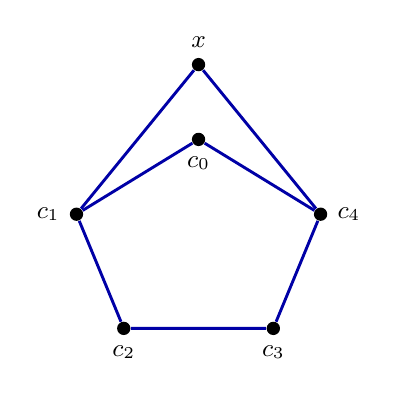
\begin{tikzpicture}[every node/.style={font=\small}]
  \node[graph vertex,label=below:$c_0$] (c0) at (0,1.4) {};
  \node[graph vertex,label=left:$c_1$] (c1) at (-1.55,0.45) {};
  \node[graph vertex,label=below:$c_2$] (c2) at (-0.95,-1) {};
  \node[graph vertex,label=below:$c_3$] (c3) at (0.95,-1) {};
  \node[graph vertex,label=right:$c_4$] (c4) at (1.55,0.45) {};
  \node[graph vertex,label=above:$x$] (x) at (0,2.35) {};
  \draw[marked edge] (c0)--(c1)--(c2)--(c3)--(c4)--(c0);
  \draw[marked edge] (c1)--(x)--(c4);
\end{tikzpicture}
\caption{A vertex $x$ in $U_0$ and its two marked edges to the cycle.}
\label{fig:odd-cycle-parts}
\end{figure}
\relax\space% End source/figures/odd_cycle_parts.tex

To express $R$ in terms of the counts, let $L_R$ be the following
linear form in the six-position coordinates. The restriction to the
first five positions is the marked induced cycle. The coefficient
of a labeled extension is the number of neighbors of the sixth
position on the cycle if that position either has an unmarked edge
to the cycle or is adjacent to two consecutive cycle positions.
All other extensions have coefficient zero. A vertex outside $B$
with a cycle neighbor satisfies at least one of these two tests.
Indeed, if it fails both, it has at most two cycle neighbors and
all edges to them are marked. With only one such neighbor $c_i$,
its marked edge to $c_i$ has no endpoint in common with the
opposite cycle edge $c_{i+2}c_{i+3}$ and no edge joins their endpoints.
With two nonconsecutive marked neighbors, it belongs to one of
the sets $U_i$. Conversely, vertices of $B$ fail both tests.

Thus the sum over the sixth position is $R$ for each ordered
cycle. The denominators in \eqref{eq:q-definition} for five and
six positions differ by a factor of $D$. If $q_C>0$, this gives
$L_R=\frac{q_C}{D}\mathbb E[R]$, where the expectation is over a
uniformly chosen color-preserving map of the cycle pattern. If $q_C=0$,
there is no such map and $L_R=0$.

The five-cycle certificates give
\begin{equation}\label{eq:odd-moment-bounds}
 \frac{\mu}{D^2}\geq\gamma_C\Bigl(\frac{1}{8}-q_C\Bigr)-\epsilon_C,
 \qquad
 \frac{\mu}{D^2}\geq\gamma_R L_R-\epsilon_R.
\end{equation}
Both errors $\epsilon_C$ and $\epsilon_R$ are nonnegative. For the
first inequality we use either
$\gamma_C\geq\frac{99999}{100000}$ and $\epsilon_C\leq2\cdot10^{-9}$,
or $\gamma_C\geq\frac{6449}{10000}$ and $\epsilon_C\leq10^{-9}$.
For the second we use $\gamma_R\geq\frac{56425}{100000}$ and
$\epsilon_R\leq10^{-9}$. The files and checks are specified in
\textbf{Appendices~\ref{app:reproduction} and~\ref{app:cycle-estimates}}.

Suppose that $\mu\leq\mu_*$, $\gamma_C\geq g_C>0$ and
$\gamma_R\geq g_R>0$. Put
$q_*=\frac{1}{8}-\frac{\mu_*+\epsilon_C D^2}{g_C D^2}$.
The first inequality in \eqref{eq:odd-moment-bounds} gives
$q_C\geq q_*$ when $q_C<\frac{1}{8}$, and the bound holds directly
when $q_C\geq\frac{1}{8}$ because $q_*\leq\frac{1}{8}$. If $q_*>0$,
using the second inequality and $L_R=\frac{q_C}{D}\mathbb E[R]$
gives a cycle with $R\leq\mathbb E[R]$ and hence
\begin{equation}\label{eq:odd-choose-anchor}
 R\leq\frac{\mu_*+\epsilon_R D^2}{g_R Dq_*}.
\end{equation}
Verified upper bounds on either error can be used in this estimate.

\begin{lemma}\label{lem:simple-cycle-counts}
For the sets defined in \eqref{eq:odd-core-defs}, every vertex of
$U_i$ is adjacent to every vertex of $U_{i+1}$. Moreover,
$|B|=\frac{5D-R}{2}$ and $a_i=\frac{D-R}{2}+s_{i-2}+s_{i+2}$ for every $i$.
\end{lemma}

\begin{proof}
Fix $x\in U_i$ and $y\in U_{i+1}$. The marked edges
$xc_{i-1}$ and $yc_{i+2}$ are disjoint because their endpoints
belong to four different parts. The strong clique property forces
at least one of $xy$, $xc_{i+2}$, $yc_{i-1}$ and
$c_{i-1}c_{i+2}$ to be an edge. By the definitions of $U_i$
and $U_{i+1}$, the two pairs $xc_{i+2}$ and $yc_{i-1}$ are
nonedges. The cycle is induced, so $c_{i-1}c_{i+2}$ is also
a nonedge. Hence $xy\in E(G)$. Consequently each vertex of $U_i$
has at most $D-a_{i-1}-a_{i+1}=s_i$ neighbors outside the two
consecutive parts.

The sum $A=\sum_i a_i s_i$ bounds the number of incidences at vertices
of $B$ after excluding the edges between $U_i$ and $U_{i+1}$ for all
$i$. Each remaining edge with both ends in $B$ contributes two
incidences. Put $e_0=\sum_i a_i a_{i+1}$, the number of edges between
parts $U_i$ and $U_{i+1}$.
Solving \eqref{eq:odd-core-defs} gives
\begin{equation}\label{eq:odd-core-sums}
 a_i=t-\frac{R}{2}+s_{i-2}+s_{i+2},\qquad
 |B|=\frac{5D-R}{2}.
\end{equation}
Summing the five equations for $s_i$ gives the formula for $|B|$.
For $a_i$, the two disjoint pairs of indices
$\{i-2,i+1\}$ and $\{i-1,i+2\}$ are the neighbor pairs of
$i+2$ and $i-2$, respectively. Subtracting their sizes from $|B|$
gives $a_i=|B|-2D+s_{i-2}+s_{i+2}$.
\end{proof}

By substituting \eqref{eq:odd-core-sums} into $\sum_i a_i s_i$
and using $2e_0=\sum_i a_i(D-s_i)$, we obtain
\begin{equation}\label{eq:odd-core-capacity}
 A=tR-\frac{R^2}{2}+2\sum_i s_i s_{i+2},
 \qquad
 e_0=5t^2-\frac{Rt+A}{2}.
\end{equation}
When $D$ is odd, $R=5D-2|B|$ is odd as well. To bound $\sum_i s_i s_{i+2}$,
consider the cycle on the indices with edges $i,i+2$. If two
nonadjacent vertices have positive weights, move their combined
weight onto the vertex with the higher sum of neighboring weights.
With the other weights fixed, the sum of products does not decrease.
Repeating leaves positive weights on a clique of size at most two.
The sum of products is then at most $\frac{R^2}{4}$. When $D$ is odd, integrality reduces this bound to $\frac{R^2-1}{4}$, so
\eqref{eq:odd-core-capacity} gives $A\leq tR-\frac{1}{2}$.

\begin{lemma}\label{lem:odd-unit-slack}
If an induced five-cycle with five marked edges has $R=1$, then $D$ is odd and $m\leq f(D)$.
\end{lemma}

\begin{proof}
Since $R=5D-2|B|=1$, the integer $D$ is odd. Let $i$ be the
unique index with $s_i=1$. For $j\ne i$, every vertex of $U_j$
has $D$ neighbors in $U_{j-1}\cup U_{j+1}$ by
\textbf{Lemma~\ref{lem:simple-cycle-counts}}. Any marked edge
whose endpoints are not in consecutive parts must therefore
have both endpoints in $U_i\cup(V(G)\setminus B)$. The marked
edge $c_{i+2}c_{i+3}$ is disjoint from such an edge, and its
endpoints have all their neighbors in $B\setminus U_i$. Thus no
edge can join their endpoints, contradicting the strong clique
property. Hence all marked edges lie between consecutive parts
and $m\leq e_0$.
For $R=1$, \eqref{eq:odd-core-capacity} gives
$A=t-\frac{1}{2}$ and $e_0=5t^2-t+\frac{1}{4}=f(D)$.
\end{proof}
\relax\space% End source/main_simple_cycle_counts.tex

\subsection{The Bound \texorpdfstring{$\frac{5}{4}\Delta^2$}{5 Delta squared / 4} in Loopless Multigraphs}
\label{sec:multigraph}\label{sec:weighted-counts}

The underlying simple graph of a multigraph records every adjacency
that can join two marked edges. To count the marked edges themselves,
we also record how many marked edges have each pair of endpoints.

Let $D\geq1$ be an integer. Take a loopless multigraph $G$ with
$\Delta(G)\leq D$ and fix a
nonempty strong clique of size $m$ in $G$. Mark the edges of the clique
and restrict $G$ to the subgraph induced by their endpoints.
For a pair joined by a marked edge, keep exactly the marked edges
with those endpoints. For any other adjacent pair, keep one
unmarked edge. Let $G_{\rm s}$ be the underlying simple graph of
the reduced multigraph. Color an edge of $G_{\rm s}$ red if its
endpoints are joined by a marked edge, and blue otherwise.
Let $s$ be the number of red edges. They form a strong clique in
$G_{\rm s}$. For each red
edge $uv$, choose one of the marked edges with endpoints $u,v$ as
its representative, and let $b_{uv}$ count the remaining marked
edges with these endpoints. Set $b_{uv}=0$ on blue edges.

Put
\[
 b=m-s,\qquad M=\frac{m}{D^2},\qquad S=\frac{s}{D^2},
 \qquad e=\frac{b}{m}.
\]
Here $M$ and $S$ are normalized clique sizes, and $e$ is the fraction
of the $m$ marked edges that remain after choosing the representatives.
Thus $S=M(1-e)$. Write
$d_{\rm s}(v)=d_{G_{\rm s}}(v)$ and
$j_v=\sum_{u\in N_{G_{\rm s}}(v)}b_{uv}$.
Then $\sum_v j_v=2b$ and $d_{\rm s}(v)+j_v\le D$.

Write $G$ for the reduced multigraph. Apply
\textbf{Lemma~\ref{lem:regularization}} to obtain a $D$-regular
multigraph $\widehat G$. Its added edges are single and unmarked.
Write $\widehat G_{\rm s}$ for its underlying simple graph, with
the new edges colored blue. The induced copy of $G$ in $\widehat G$
has the original marked edges with their multiplicities.

Use the weighted patterns of
\textbf{Subsection~\ref{subsec:weighted-sketch}}, writing $(P,T)$
for a colored pattern on $n$ positions and its set of specified
pairs. We take $P$ to be connected with at least one red edge.
As in \textbf{Definition~\ref{def:patterns}},
any two red edges in $P$ either meet or have endpoints joined by a red
or blue edge. In the weighted counts, $P$ has no designated root edge.
Define
\begin{equation}\label{eq:weighted-count}
 Q(P,T)=\frac{1}{2mD^{n-2}}
       \sum_{\phi}\ \prod_{uv\in T} b_{\phi(u)\phi(v)},
 \qquad
 X(P,T)=\frac{Q(P,T)}{|\operatorname{Aut}(P,T)|}.
\end{equation}
Here $\phi$ runs over color-preserving maps of the positions of $P$
to $\widehat G_{\rm s}$, and $\operatorname{Aut}(P,T)$ is the group of
permutations of the positions that preserve the pair colors and the
edge set $T$. As before, color $0$ permits equal images. Each pair
$uv$ in $T$ contributes its own factor $b_{\phi(u)\phi(v)}$, even
if two pairs have the same images, as in
\textbf{Figure~\ref{fig:weighted-maps}}.
The forest condition is imposed on the positions. We use patterns
with $2\le n\le6$ and $|T|\le3$. Write $X$ for the vector of coordinates
$X(P,T)$, using one representative for each isomorphism class of pairs
$(P,T)$.

% Begin source/figures/weighted_maps.tex
\begin{figure}[htbp]
\centering
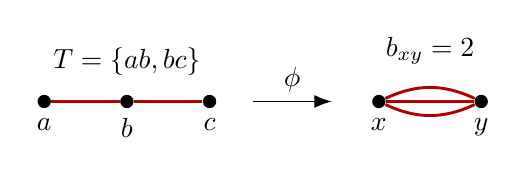
\begin{tikzpicture}[marked edge/.append style={draw=red!70!black}]
  \node[graph vertex,label=below:$a$] (a) at (0,0) {};
  \node[graph vertex,label=below:$b$] (b) at (1.05,0) {};
  \node[graph vertex,label=below:$c$] (c) at (2.1,0) {};
  \draw[marked edge] (a)--(b)--(c);
  \node[above=6pt] at (b) {$T=\{ab,bc\}$};
  \draw[-{Latex[length=2.2mm]}] (2.65,0)--node[above]{$\phi$}(3.65,0);
  \node[graph vertex,label=below:$x$] (x) at (4.25,0) {};
  \node[graph vertex,label=below:$y$] (y) at (5.55,0) {};
  \draw[marked edge] (x)--(y);
  \draw[marked edge] (x) to[bend left=25] (y);
  \draw[marked edge] (x) to[bend right=25] (y);
  \node[above=10pt] at (4.9,0) {$b_{xy}=2$};
\end{tikzpicture}
\caption{A weighted map with $\phi(a)=\phi(c)=x$ and $\phi(b)=y$.
Its weight is $b_{xy}^2=4$.}
\label{fig:weighted-maps}
\end{figure}
\relax\space% End source/figures/weighted_maps.tex

For the pattern $P$ consisting of a single red edge, summing over the
$2s$ ordered red edges of the underlying simple graph gives
$Q(P,\varnothing)=1-e$. Summing $b_{uv}$ over these ordered edges
gives $Q(P,E(P))=e$, where $E(P)$ consists of the single red pair.
To form a degree identity, fix $(P,T)$ and a position $u$ of $P$.
For each color-preserving map $\phi$ in \eqref{eq:weighted-count},
choose one of the $D$ edges of $\widehat G$ incident with $\phi(u)$
and send the new position to its other endpoint. When the edge is
unmarked or a representative, retain $T$. When it is a remaining
marked edge, add the pair joining $u$ to the new position to the
specified set. This is the count from
\textbf{Subsection~\ref{subsec:weighted-uniform-sketch}}. Use the
identity for $(P,T),u$ when all its terms occur in the model.

Choose two ordered marked edges independently, allowing the same
edge in both choices. There are $(2s)^2$ ordered pairs of
representatives, $2(2s)(2b)$ ordered pairs with exactly one
representative, and $(2b)^2$ ordered pairs with neither edge a
representative. Each choice determines the images of four positions
in the underlying simple graph. Their colors give a connected
pattern because the two edges belong to the strong clique.
For each specified pair, the factor $b_{uv}$ counts the choices of
a remaining marked edge with the given endpoints. As in
\eqref{eq:objective-vector}, divide the counts by $2mD^2$ and take
one half. The three contributions to the objective are
\[
 O_0=\frac{s^2}{mD^2},\qquad
 O_1=\frac{2sb}{mD^2},\qquad
 O_2=\frac{b^2}{mD^2}.
\]
Their sum is $M$ since $m=s+b$. More generally, adding an independent
ordered marked edge to a fixed pattern gives $2M Q(P,T)$ after
normalization. The choice of an ordered marked edge multiplies the
raw count by $2m$, and the two new positions contribute a factor
$D^2$ in the denominator. If we choose only from the representatives
or only from the remaining marked edges, the corresponding factors
give $2S Q(P,T)$ and $2Me Q(P,T)$. These formulas give linear bounds
when $M$, $S$ and $e$ are restricted to intervals.
For example, the bounds $e_-\le e\le e_+$ imply
\[
 O_2\le(e_-+e_+)\left(O_2+\frac{O_1}{2}\right)-e_-e_+M
\]
by expanding $M(e-e_-)(e_+-e)\ge0$.

Fix a weighted type $(T_0,J_0)$ on $k$ positions and a sequence
of weighted flags $(F_i,J_i)$ of that type, with $F_i$ on $n_i$
positions. For a map $\phi$ giving the colors of $T_0$, set
\[
 w(\phi)=\prod_{\{u,v\}\in J_0}b_{\phi(u)\phi(v)},\qquad
 v_i(\phi)=\frac{1}{D^{n_i-k}}
    \sum_g\prod_{\{u,v\}\in J_i\setminus J_0}b_{g(u)g(v)},
\]
where the sum for $v_i(\phi)$ runs over the extensions $g$ of $\phi$
giving the colors of $F_i$. Let $v(\phi)$ be the column vector
with entries $v_i(\phi)$. Then
\[
 \frac{1}{2mD^{k-2}}\sum_\phi w(\phi)v(\phi)v(\phi)^{\mathsf T}\succeq0.
\]
The matrix is a sum of outer products with nonnegative coefficients,
since $w(\phi)\geq0$ for every $\phi$. To compute its $(i,j)$ entry,
combine the position sets of the two flags using
\eqref{eq:flag-relabeling}, so that they meet exactly on $P_k$.
Their extensions of $\phi$ define a common map on the union.
The factor $w(\phi)$ counts the choices on $J_0$ once, and the
two extension factors count the choices on their other specified
pairs. The product has denominator $2mD^{n_i+n_j-k-2}$.
Grouping the maps by their colors on the union, as in
\textbf{Subsection~\ref{subsec:weighted-sketch}}, therefore expresses
the entry as a linear combination of the $Q(P,T)$ and hence of
the $X(P,T)$. We choose the flags so that each resulting weighted
pattern belongs to the specified collection.
The same counting identity applies to the matrices formed from local
degrees and from counts of extensions satisfying degree constraints.

% Begin source/main_multigraph_cycle_counts.tex
To bound $M$ we also need to count the edges at the vertices of an
induced red five-cycle in the reduced multigraph. Use the parts $U_i$
and remaining degrees $s_i$ from \eqref{eq:odd-core-defs} for the red
edges of its underlying simple graph. Call the vertices $c_0,\ldots,c_4$ of
the cycle its anchors, with indices modulo five, and put
$B=\bigcup_i U_i$. We call $B$ the core of this cycle.
Let $L$ be the number of blue pairs between $U_i$ and $U_{i+1}$,
summed over $i$. By \textbf{Lemma~\ref{lem:simple-cycle-counts}},
all pairs between these two parts are adjacent. Reserving one edge
for each such pair leaves at most $s_i$ incidences at each vertex of
$U_i$. Set $a_*=\frac{D-R}{2}$. Equations \eqref{eq:odd-core-sums}
and \eqref{eq:odd-core-capacity} applied to the underlying simple graph give
\begin{equation}\label{eq:multi-core-identities}
 a_i=a_*+s_{i-2}+s_{i+2},\qquad
 A=\sum_i a_is_i=\frac{RD}{2}-\frac{R^2}{2}
             +2\sum_i s_i s_{i+2}\le\frac{RD}{2}.
\end{equation}
In particular $R=5D-2|B|$ has the same parity as $D$.

We now bound the contribution of edges incident with vertices outside $B$.
Set $r=\frac{R}{D}$, $j=\frac{\sum_{i=0}^4j_{c_i}}{D}$,
$g=\frac{m}{D^2}-\frac{5}{4}$, and $\lambda=\frac{L}{D^2}$.

\begin{lemma}\label{lem:multigraph-cycle-counts}
If $g>0$, then $r>\frac{1}{2}$. For $\frac{1}{2}\le r\le1$,
\begin{equation}\label{eq:multi-joint}
 2g+2\lambda\le
 \frac{1+r}{2+r}\,r\left(r-\frac{1}{2}\right)
 -\frac{1+r^2}{2+r}\,j.
\end{equation}
\end{lemma}
\begin{proof}
For each vertex $x$, define its \emph{signature}
$I_x=\{i:xc_i\in E(G_{\rm s})\}$ and put $k_x=|I_x|$. Let
$K=\sum_{x\notin B}k_x$, the number of adjacent pairs with one
endpoint among the $c_i$ and the other outside $B$. The bounds
$s_i$ on the degrees from $c_i$ to $V(G)\setminus B$ give
$K\leq\sum_i s_i=R$. For $x\notin B$, let $h_x$ be its marked
degree, put $Q_x=|N_{G_{\rm s}}(x)\cap B|$, and let $b_x$ be the
number of blue edges from $x$ to $B$.

For every marked edge $xy$, the set $\{c_i:i\in I_x\cup I_y\}$ is
a vertex cover of the cycle, that is, it meets every cycle edge.
Indeed, if a cycle edge is disjoint from $xy$, the strong clique
property gives an edge from $x$ or $y$ to an endpoint of that cycle
edge. If the two edges share an endpoint, the other endpoint of the
cycle edge is a neighbor of the shared endpoint. A vertex cover of
$C_5$ has at least three vertices. Thus if $k_x=0$, every marked
neighbor $y$ of $x$ satisfies $k_y\geq3$. In particular, $x$ has no
marked neighbor in $B$, because every vertex of $B$ has signature
size two.

If $x\notin B$ has $k_x=2$, at least one of its two edges to the
cycle is blue. For $I_x=\{i,i+1\}$, the marked edge $xc_i$ would
have no edge joining its endpoints to those of $c_{i+2}c_{i+3}$.
The same argument for $xc_{i+1}$ uses $c_{i+3}c_{i+4}$. For
$I_x=\{i-1,i+1\}$, if both edges were marked, $x$ would be in
$U_i\subseteq B$.

To bound the sum of the marked degrees over $B$, subtract the
incidences of these unmarked edges from the degree bound $D|B|$.
Each of the $L$ blue edges between consecutive parts has two
incidences at $B$. Each blue edge from $x\notin B$ to $B$ has
one, counted by $b_x$. These two classes of edges are disjoint.
\textbf{Figure~\ref{fig:multigraph-cut}} shows both cases.
Adding the marked degrees outside $B$ gives
\begin{equation}\label{eq:multi-core-cut}
 2m\le D|B|-2L+\sum_{x\notin B}(h_x-b_x).
\end{equation}

% Begin source/figures/multigraph_cut.tex
\begin{figure}[htbp]
\centering
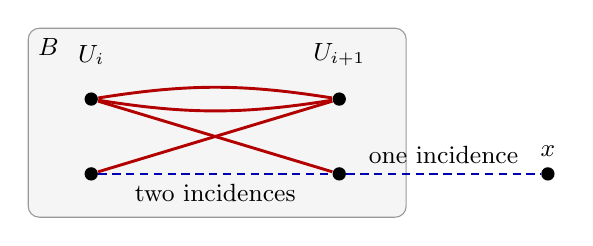
\begin{tikzpicture}[
  marked edge/.append style={draw=red!70!black},
  blue pair/.style={draw=blue!70!black,densely dashed,line width=0.95pt},
  font=\small
]
  \filldraw[fill=black!4,draw=black!40,rounded corners=4pt]
    (-0.65,-0.55) rectangle (4.15,1.85);
  \node[anchor=north west] at (-0.65,1.85) {$B$};
  \node at (0.15,1.51) {$U_i$};
  \node at (3.3,1.51) {$U_{i+1}$};
  \node[graph vertex] (a) at (0.15,0.95) {};
  \node[graph vertex] (b) at (0.15,0) {};
  \node[graph vertex] (c) at (3.3,0.95) {};
  \node[graph vertex] (d) at (3.3,0) {};
  \node[graph vertex,label=above:$x$] (x) at (5.95,0) {};
  \draw[marked edge] (a) to[bend left=9] (c);
  \draw[marked edge] (a) to[bend right=9] (c);
  \draw[marked edge] (a)--(d);
  \draw[marked edge] (b)--(c);
  \draw[blue pair] (b)--node[below] {two incidences} (d);
  \draw[blue pair] (d)--node[above] {one incidence} (x);
\end{tikzpicture}
\caption{A blue edge between consecutive parts contributes twice to
the degree sum on $B$. A blue edge from $x\notin B$ to $B$ contributes
once. Both marked edges with the same endpoints contribute to marked degree.}
\label{fig:multigraph-cut}
\end{figure}
\relax\space% End source/figures/multigraph_cut.tex

We first establish two bounds on the neighbors in $B$ of vertices
outside $B$. Suppose $x\notin B$ has $I_x=\{j\}$ and a marked edge
$xy$ with $y\in U_i$. The set $\{j,i-1,i+1\}$ covers the cycle,
which requires $i=j+2$ or $i=j-2$. Exactly one of $c_{j-1}$ and
$c_{j+1}$ is nonadjacent to $y$. Call it $c_k$. For each $u\in U_j$,
the marked edges $xy$ and $c_ku$ are disjoint, and $c_k$ is
adjacent to neither $x$ nor $y$. The strong clique property
therefore gives $xu\in E(G_{\rm s})$ or $yu\in E(G_{\rm s})$.
Since $U_j$ is nonconsecutive to $U_i$, the edge $xy$ and the
edges from $y$ to $U_j$ use the same $s_i$ available incidences.
It follows that at most $s_i-1$ vertices of $U_j$ are adjacent to
$y$, so at least $a_j-s_i+1\geq a_*+1$ are adjacent to $x$.
All these edges from $x$ are blue because $\{j,j-1,j+1\}$ does not
cover the cycle. Hence $b_x\geq a_*+1$.

Now suppose $xy$ is a marked edge with both endpoints outside $B$
and $|I_x\cup I_y|=3$. The two omitted indices are nonconsecutive
because $I_x\cup I_y$ covers the cycle. Write them as $i,i+2$,
after interchanging them if necessary. For each
$u\in U_{i-1}\cup U_{i+1}\cup U_{i+3}$, at least one of $c_i u$
and $c_{i+2}u$ is marked. Neither $c_i$ nor $c_{i+2}$ is adjacent
to $x$ or $y$, so the strong clique property implies
$u\in N_{G_{\rm s}}(x)\cup N_{G_{\rm s}}(y)$. The two remaining
parts $U_i,U_{i+2}$ have total size at most $D$ because every
vertex in them is adjacent to $c_{i+1}$. Thus
\[
 Q_x+Q_y\geq |B|-D=D+a_*.
\]
Since the edge $xy$ uses a degree at each endpoint outside $B$,
we have $Q_x,Q_y\leq D-1$, so $Q_x,Q_y\geq a_*+1$. In particular,
if $k_x=1$, $k_y=2$, and $x$ has no marked neighbor in $B$, then
all these edges from $x$ to $B$ are blue and $b_x\geq a_*+1$.

Suppose $R\leq D$. To bound the sum in \eqref{eq:multi-core-cut},
assign each $x\notin B$ the initial value $h_x-b_x$ and transfer
part of that value along marked edges between vertices outside $B$.
The sum is preserved by each transfer.

If $k_x=1$ and $x$ has a marked neighbor in $B$ or a marked neighbor
with signature size two, the preceding bounds give $b_x\geq a_*+1$.
Since $h_x+b_x\leq D$, its initial value is at most
$D-2(a_*+1)=R-2$. Make no transfer from such a vertex. Every other
vertex $x$ with $k_x=1$ sends $\frac12$ along each of its marked
edges. All these edges join it to a vertex outside $B$ with
signature size at least three. The value left at $x$ is
$\frac{h_x}{2}-b_x\leq\frac D2$.

If $k_x=0$ and $h_x-b_x>0$, send
$\frac{h_x-b_x}{h_x}$ along each marked edge at $x$.
If $x$ has a marked neighbor with signature size three, the bound
from the two omitted anchors gives $b_x=Q_x\geq a_*$. Since
$h_x\leq D-Q_x$, the amount on each edge is at most
\[
 1-\frac{a_*}{D-a_*}=\frac{2R}{D+R}.
\]
If all marked neighbors of $x$ have signature size at least four,
the amount is at most one on each edge. Vertices of signature size
zero with nonpositive initial value make no transfers. In either
case the value left at a vertex of signature size zero is at most
zero.

A vertex $x$ with $k_x=3$ and a marked neighbor with signature
size zero satisfies $Q_x\geq a_*$ by the bound for the three
parts. It has at most $\frac{D+R}{2}$ marked edges to vertices
outside $B$. The amount received on each is at most
$\max\{\frac12,\frac{2R}{D+R}\}$, so the total received is at
most $\max\{\frac{D+R}{4},R\}$. A vertex with $k_x=3$ and no
marked neighbor with signature size zero receives at most
$\frac D2$. Since $R\leq D$, in both cases its initial value
plus the amount received is at most
$D+\max\{\frac D2,R\}\leq k_x\max\{\frac D2,R\}$.
If $k_x\geq4$, the amount received is at most $D$, so its
final value is at most $2D\leq k_x\max\{\frac D2,R\}$.
A vertex with $k_x=2$ receives nothing and has initial value
at most $D$. Together with the bounds for $k_x=0,1$, this
gives $k_x\max\{\frac D2,R\}$ as an upper bound for the final
value at every $x\notin B$. By \eqref{eq:multi-core-cut},
\begin{equation}\label{eq:multi-rough-discharge}
2m\le D|B|-2L+\max\left\{\frac{D}{2},R\right\}K.
\end{equation}

If $R\le \frac{D}{2}$, the right-hand side of \eqref{eq:multi-rough-discharge}
is at most $D|B|+\frac{D}{2}R=\frac{5}{2}D^2$.
Thus $g>0$ implies $r>\frac{1}{2}$.

Assume now that $\frac{1}{2}\le r\le1$. The $K$ adjacencies from the
five cycle vertices to the exterior and the $\sum_i j_{c_i}$ incidences
of the remaining marked edges at those vertices use disjoint units of the remaining
degree $R$. Thus $K\le R-\sum_i j_{c_i}$.
For the refined bound, divide vertex counts and individual degrees
by $D$ and divide edge counts and sums of degrees by $D^2$.
Write $\eta=\frac{1-r}{2}$, $v=\frac{1+r}{2}$ and
$\rho=\frac{2r}{1+r}$. If a marked edge has both endpoints
outside $B$ and the union of their signatures has size three,
the normalized degree from each endpoint to $B$ is at least
$\eta=\frac{a_*}{D}$. Its normalized marked degree to vertices
outside $B$ is at most $v=1-\eta$.

Let $X_1$ consist of vertices outside $B$ of signature size one
that have a marked neighbor in $B$ or a marked neighbor of
signature size two. Write
\[
 x=\frac{|X_1|}{D},\qquad
 C_1=\frac{1}{D^2}\sum_{y\in X_1}(h_y-b_y).
\]
Each vertex of $X_1$ has normalized blue degree to $B$ at least
$\eta$ and normalized contribution $(h_y-b_y)/D$ at most $r$,
so $C_1\leq rx$. Let $p_2$ and $p_3$ count, in normalized units,
marked edges from $X_1$ to vertices outside $B$ with signature size
two and with signature size at least three, respectively. Let $n_2$
be the normalized number of signature-size-two endpoints of the
edges counted by $p_2$. Let $z_0$ and $z_3$ be the normalized
numbers of endpoints of signature sizes zero and three among
marked edges joining these two groups. Write $p_{03}$ for the
normalized number of those edges. The three groups counted by
$n_2,z_0,z_3$ are disjoint. Each vertex in any of these groups
has normalized degree to $B$ at least $\eta$ and normalized
marked degree outside $B$ at most $v$, since it is an endpoint
of an edge with union of signatures of size three. Hence
$p_2\leq v n_2$ and $p_{03}\leq v\min\{z_0,z_3\}$.

By \eqref{eq:multi-core-identities}, the normalized degree
available at $B$ after reserving the edges between consecutive
parts is at most $\frac{r}{2}$. The blue edges from $X_1$ to $B$
use at least $\eta x$ of this degree. The edges from the groups
counted by $n_2,z_3,z_0$ to $B$ use at least
$\eta(n_2+z_3+z_0)$. The remaining degree bounds the normalized
number of marked edges from $X_1$ to $B$. To bound $C_1$, add
$p_2+p_3$ for the marked edges from $X_1$ to vertices outside
$B$ and subtract another $\eta x$ for the terms $-b_y$ with
$y\in X_1$. This gives
\[
 C_1\leq\frac{r}{2}-2\eta x-\eta(n_2+z_3+z_0)+p_2+p_3.
\]
Set $\theta=\frac{2r-1}{2+r}$ and
$c=r-\theta=\frac{1+r^2}{2+r}$. Since $0\leq\theta\leq\frac13$,
we can multiply the first bound $C_1\leq rx$ by $1-\theta$ and
the latter bound by $\theta$ and add. Using $r+2\eta=1$ gives
\begin{equation}\label{eq:multi-joint-first}
 C_1\le cx+\frac{\theta r}{2}
     +\theta(p_2+p_3)-\theta\eta(n_2+z_3+z_0).
\end{equation}

Use the same transfers as in \eqref{eq:multi-rough-discharge}
for vertices outside $B$ and outside $X_1$. A vertex with signature
size two has normalized contribution at most one. Assign the
terms $\theta p_2-\theta\eta n_2$ of
\eqref{eq:multi-joint-first} to the vertices counted by $n_2$.
Since $p_2\leq v n_2$ and $v-\eta=r$, the bound on their total
contribution becomes $(1+\theta r)n_2=2c n_2$.
The other vertices with signature size two already satisfy this
bound per two signature positions because $c\geq\frac12$.

For a vertex outside $B$ with signature size at least three, let
$d_1$ be its normalized marked degree to $X_1$. Transfers are zero
on those edges. If the signature has size at least four, each of
the other incident marked edges contributes at most one through
a transfer. Adding the vertex's own normalized contribution,
at most one, gives at most $2-d_1$. If the signature has size three
and the vertex has no marked neighbor of signature size zero,
each transfer is at most $\frac12$, giving
$\frac32-\frac{d_1}{2}$. Adding the term $\theta d_1$ from
$\theta p_3$ to each bound gives at most $2$ or $\frac32$,
respectively, because $\theta\leq\frac13$. Both bounds are at most
$c$ times the corresponding signature size.

For the group counted by $z_3$, write $d_{1,3}$ for the normalized
number of marked edges from the group to $X_1$. Each vertex
has normalized marked degree outside $B$ at most $v$. Transfers
are zero from $X_1$, at most $\rho$ per edge from the group counted
by $z_0$, and at most $\frac12$ per other edge. Thus the normalized
amount received is at most
$\frac12(vz_3-d_{1,3}-p_{03})+\rho p_{03}$. To bound the total,
add $z_3$ for their own contributions and add
$\theta d_{1,3}-\theta\eta(z_3+z_0)$ from
\eqref{eq:multi-joint-first}. This gives
\[
 \left(1+\frac{v}{2}\right)z_3
 -\left(\frac{1}{2}-\theta\right)d_{1,3}
 +\left(\rho-\frac{1}{2}\right)p_{03}-\theta\eta(z_3+z_0).
\]
Discard the nonpositive term containing $d_{1,3}$ and substitute
$z_0\geq\frac{p_{03}}{v}$. The resulting coefficient of $p_{03}$
is $\rho-\frac12-\frac{\theta\eta}{v}\geq0$, since
$\rho\geq\frac23$ and $\frac{\theta\eta}{v}\leq\frac19$.
Thus substituting $p_{03}\leq v z_3$ gives the bound
$(1+\rho v-2\theta\eta)z_3=3c z_3$.

The remaining vertices of signature size one have normalized
contribution at most $\frac12\leq c$, and those of signature size
zero have contribution at most zero. Including the $cx$ in
\eqref{eq:multi-joint-first}, we have bounded the normalized
sum outside $B$ by $cK/D+\frac{\theta r}{2}$. Substitute this
bound and $K\leq R-\sum_i j_{c_i}$ into \eqref{eq:multi-core-cut}
and divide the degree terms there by $D^2$. Since
$|B|/D=\frac{5-r}{2}$, this gives
\[
 \frac{2m}{D^2}\leq\frac{5-r}{2}-2\lambda+c(r-j)
                   +\frac{\theta r}{2}.
\]
Subtract $\frac52$ and use
$c+\frac{\theta}{2}-\frac12=\frac{1+r}{2+r}(r-\frac12)$
to obtain \eqref{eq:multi-joint}.

\end{proof}
\relax\space% End source/main_multigraph_cycle_counts.tex

% Begin source/main_flag_bounds.tex
Apply the simple-graph five-cycle counts to the red edges of
$G_{\rm s}$. Completing the underlying simple graph to a $D$-regular simple
graph adds only blue edges. All vertices of a red five-cycle and of
its five parts are incident with red edges. They therefore belong
to the old graph, which is induced in the completion. Thus the
completion preserves both the red five-cycles and their five
parts. Write $q_C$ for the number of ordered induced red five-cycles
divided by $2sD^3$ and $L_R$ for the sum of $\frac RD$ over these
cycles divided by the same quantity. If each such cycle satisfies
$R\geq\alpha D$, then summing this inequality gives $L_R\geq\alpha q_C$.

Applying the simple-graph certificate inequality to four choices
of objective gives
\begin{equation}\label{eq:support-projection-four}
\begin{aligned}
 S-0.99999q_C
   &\le \frac{5}{4}-\frac{0.99999}{8}+2\cdot10^{-9},\\
 S+0.5682L_R
   &\le \frac{5}{4}+10^{-9},\\
 S+0.4897(L_R-0.32q_C)
   &\le \frac{5}{4}-\frac{0.4897\cdot0.32}{8}+2\cdot10^{-9},\\
 S+0.45119\left(L_R-\frac{q_C}{2}\right)
   &\le \frac{5}{4}-\frac{0.45119}{16}+2\cdot10^{-9}.
\end{aligned}
\end{equation}
The coefficients and the error allowances in
\eqref{eq:support-projection-four} are rational.
\textbf{Appendix~\ref{app:multi-projection}} specifies the
four certificate checks. To see why the displayed coefficients
suffice, write each certified inequality as $S+\gamma Y\leq
\frac54+\varepsilon$, moving the multiple of $\frac18$ to the left.
For $Y\geq0$, replacing $\gamma$ by a smaller nonnegative coefficient
preserves the inequality. For $Y<0$ the bound follows from
$S\leq\frac54$.

For a given $\alpha>0$, substitute $L_R\geq\alpha q_C$ in
\eqref{eq:support-projection-four}. Each of the four inequalities
now has the form $S\leq a_i-b_iq_C$. Include $S\leq\frac54$ as
a fifth inequality, with $a_5=\frac54$ and $b_5=0$. Thus
\[
 S\leq S_{\max}(\alpha):=
 \max_{x\geq0}\min_{1\leq i\leq5}(a_i-b_ix),
 \qquad e\geq1-\frac{S_{\max}(\alpha)}{M}.
\]
The second line of \eqref{eq:support-projection-four} has
$b_2=0.5682\alpha>0$. The minimum of the five lines is continuous
and piecewise linear and tends to $-\infty$ as $x$ tends to infinity.
Its maximum is therefore attained at zero or at the nonnegative
intersection of two lines with different slopes. This gives a finite
rational calculation for $S_{\max}(\alpha)$.

These inequalities can also be imposed directly on $X$. Multiplying
each simple-graph inequality by $1-e=\frac{s}{m}$ changes the cycle
normalization from $2sD^3$ to $2mD^3$. Its term $(1-e)S$ is $O_0$,
and the same factor changes $L_R$ to the corresponding weighted
coordinate sum. All terms of the resulting inequality are linear
in the weighted counts.

To bound the size of a red clique, let $K$ be the vertex set of
a red $K_k$ in $\widehat G_{\rm s}$, with $k\geq3$. For each
vertex $v$ put $a_v=|N_{\widehat G_{\rm s}}(v)\cap K|$ and let
$h_v$ and $d_{\rm blue}(v)$ count the marked and unmarked edges
incident with $v$ in $\widehat G$, respectively. Let $m_K$ be
the number of marked edges with both endpoints in $K$, counting
multiplicity, and put $J_K=\sum_{v\in K}j_v$. A vertex added in
the completion has $j_v=0$.

For a marked edge $uv$, the set
$(N_{\widehat G_{\rm s}}(u)\cup N_{\widehat G_{\rm s}}(v))\cap K$
is a vertex cover of the red clique. If an edge of that clique
is disjoint from $uv$, it has an endpoint adjacent to $u$ or $v$
by the strong clique property. If it shares an endpoint with
$uv$, its other endpoint is adjacent to the shared endpoint.
A vertex cover of $K_k$ has size at least $k-1$. Thus
$a_u+a_v\geq k-1$ for every $uv$. If exactly one endpoint,
say $u$, lies in $K$, then $a_u=k-1$ and $a_v\geq1$. If both
lie in $K$, then $a_u+a_v=2(k-1)$. Equivalently, the lower bound
on $a_u+a_v$ is $k-1$ plus the number of endpoints in $K$, and
an additional $k-3$ when both endpoints lie in $K$. Summing these
lower bounds over the marked edges yields the first inequality in
\[
 (k-1)m+\sum_{v\in K}h_v+(k-3)m_K
 \le\sum_v a_vh_v
 \le D(kD-J_K)-\sum_{v\in K}d_{\rm blue}(v).
\]
For the upper bound, $\sum_v a_v=\sum_{v\in K}(D-j_v)=kD-J_K$.
If $v$ has a blue neighbor in $K$, then $a_v\geq1$, so
$a_vd_{\rm blue}(v)$ bounds the number of its blue neighbors
in $K$. If it has no blue neighbor in $K$, the same bound holds
by nonnegativity. Summing over $v$ gives
$\sum_v a_vd_{\rm blue}(v)\geq\sum_{v\in K}d_{\rm blue}(v)$.
Since $h_v=D-d_{\rm blue}(v)$, this gives the upper bound.
Using $\sum_{v\in K}(h_v+d_{\rm blue}(v))=kD$ now gives
\[
 (k-1)m\le kD(D-1)-DJ_K-(k-3)m_K.
\]
For $k=5$, the right side is at most $5D(D-1)-20$. Thus a red $K_5$
implies
\begin{equation}\label{eq:red-k5-bound}
 4m\leq5D(D-1)-20.
\end{equation}
This is impossible when $m\geq\frac54D^2$. For odd $D$ it is also
impossible when $m=f(D)+1$, since then $4m=5D^2-2D+5$.
The coordinates of every pattern containing a red $K_5$ are
therefore zero in either case.

We adapt the construction of a bipartite subgraph in Faron and
Postle~\cite{FaronPostle2019} to the marked
multigraph. Fix a red edge $xy$ and set
\[
 U=N_{G_{\rm s}}(x)\setminus(N_{G_{\rm s}}(y)\cup\{y\}),
 \qquad
 W=V(G)\setminus(N_{G_{\rm s}}(x)\cup N_{G_{\rm s}}(y)).
\]
Take the induced host $G[U\cup W]$ and mark only the previously
marked edges between $U$ and $W$. These edges still form a strong
clique in the induced host because every adjacency between their
endpoints is retained. Let $\sigma$ be their Ore-degree in this
host when the marked set is nonempty.

For a marked edge $uv$ between $U$ and $W$, fix a red neighbor
$z$ of $y$. Neither $u$ nor $v$ is adjacent to $y$, and $z$ lies
outside $U\cup W$. The strong clique property for $uv$ and a marked
edge with endpoints $y,z$ therefore requires $uz$ or $vz$ to be
a host edge before taking the induced subgraph. Distinct red
neighbors $z$ give distinct incidences lost from the degree sum
at $u,v$. The original degree sum is at most $2D$. Thus $\sigma$
is at most $2D$ minus the number of red neighbors of $y$.

If there is a marked edge between $U$ and $W$, the corresponding
upper bounds are
\[
 \begin{array}{ll}
 \frac{2973}{10000}\sigma^2 & \text{for all marked edges},\\
 \frac{273323}{10^6}\sigma^2 & \text{for the representatives},\\
 \frac{1}{4}\sigma^2 & \text{for the remaining marked edges}.
 \end{array}
\]
For the bound on all marked edges, adapt the neighborhood count
of Kumar, Mohar and Pragada~\cite{KumarMoharPragada2026}
to parallel marked edges. Write $G'$ for the induced host and
$H$ for its bipartite marked subgraph, counting parallel edges
separately. We also use the following count when the host or its
set of marked edges is restricted. Suppose $H$ is nonempty and its
Ore-degree in $G'$ is at most $\sigma$. Choose $v$ with
$d_H(v)=h=\Delta(H)$. Set
\[
 A=N_H(v),\qquad B'=V(G')\setminus N_{G'}[v],
 \qquad p=|A|,\qquad \ell=\sigma-d_{G'}(v).
\]
For each $a\in A$, a marked edge joins $v$ and $a$, so
$d_{G'}(a)\leq\ell$. Let $T$ count the marked edges meeting $A$,
let $P$ count the unmarked edges between $A$ and $B'$, and put
$F=H[B']$, $f=|E(F)|$ and $u=\Delta(F)$, with $u=0$ if $F$ has
no edges. A marked edge outside the two groups counted by $T$
and $f$ has an endpoint in $N_{G'}(v)\setminus A$. These neighbors
use distinct incidences at $v$ in addition to its $h$ marked
incidences. Thus there are at most $d_{G'}(v)-h$ such neighbors
and each has marked degree at most $h$. The edges counted by
$T+P$ are incident with $A$, whose degree sum is at most $p\ell$.
Consequently
\[
 |E(H)|\leq h(\sigma-h)-h\ell+T+f,\qquad T+P\leq p\ell .
\]
For each $a\in A$ and each marked edge $xy$ of $F$, neither $x$
nor $y$ is adjacent to $v$. Thus the strong clique property for
$xy$ and a marked edge from $v$ to $a$ forces $a$ to meet an
endpoint of $xy$ by an edge. The neighbors of $a$ in $B'$
therefore cover all edges of $F$. The set of these neighbors
has size at most $\ell$ and each has degree in $F$ at most $u$,
so $f\leq u\ell$. Also, for each of the $p$ vertices of $A$,
at least one edge to $x$ or $y$ is lost on restricting the host
to $B'$. The Ore-degree of $F$ in $G'[B']$ is therefore at most
$\sigma-p$ when $f>0$.

First bound the number of all marked edges. On each pair joined
by a marked edge, remove the unmarked edges. On every other
adjacent pair retain one unmarked edge. This preserves the marked
edge set and all adjacencies, and the degree sums on marked edges
are still bounded by $\sigma$. Use the preceding notation for
this reduced host. Let $X'$ consist of the vertices of $B'$ in
the same part of $H$ as $v$. For $x\in X'$, let $h_x$ count the
marked edges from $x$ to $A$, with multiplicity, and put
$f_x=d_F(x)$.

For each pair consisting of $a\in A$ and an edge of $F$, at least
one edge joins $a$ to an endpoint of that edge of $F$. Each of the
$P$ unmarked edges from $A$ to $B'$ accounts for at most $u$ such
pairs. A marked edge from $A$ to $B'$ has its endpoint $x\in X'$,
since $H$ is bipartite. The $h_x$ marked edges from $A$ to $x$
account for at most $h_x f_x$ such pairs. Therefore
\[
 pf\leq uP+\sum_{x\in X'} h_xf_x .
\]
Since $T\geq h>0$, if $f>0$ we can set
$\alpha=\frac{T}{T+f}$ and $\gamma=\frac{f}{T+f}$.
The identity
$(h_x+f_x)(\gamma^2h_x+\alpha^2 f_x)-h_x f_x
=(\gamma h_x-\alpha f_x)^2$ and the bound $h_x+f_x\leq h$
give $\sum_{x\in X'} h_xf_x\leq h(\gamma^2T+\alpha^2 f)
=\frac{hTf}{T+f}$, using $\sum_{x\in X'}h_x\leq T$
and $\sum_{x\in X'}f_x=f$. Since $f>0$ implies $u>0$,
$P\geq\frac{1}{u}(pf-\frac{hTf}{T+f})$. Substitute this bound
into $T+P\leq p\ell$ and use the resulting lower bound on $\ell$
in the inequality for $|E(H)|$ to obtain
\[
 |E(H)|\leq h(\sigma-h)+\left(1-\frac hp\right)T
       +\left(1-\frac hu\right)f
       +\frac{h^2Tf}{pu(T+f)} .
\]
If $f=0$, use $T\leq p\ell$ and $p\leq h$ in the first bound
on $|E(H)|$ to obtain $|E(H)|\leq h(\sigma-h)$.
The induced host on $B'$ has fewer marked edges, since it omits
all marked edges at $v$. Applying bounds for this smaller graph with
Ore-degree at most $\sigma-p$ gives upper bounds for $f$.
The proof notes in the repository~\cite{FGSTCode} give further necessary
inequalities by comparing the marked neighborhoods in $A$ of
two vertices of $X'$. For example, if $x,x'\in X'$ are nonadjacent,
every vertex of $N_H(x)\cap A$ that is not adjacent to $x'$ must
be adjacent to every vertex of $N_H(x')\cap A$ that is not adjacent
to $x$. Otherwise two marked edges would have no edge joining their
endpoints. The rational interval check in \textbf{Appendix~\ref{app:ore-replay}}
uses these neighborhood inequalities and the bounds for the smaller
graph. It excludes $|E(H)|>\frac{2973}{10000}\sigma^2$ over the full
range of $\frac{h}{\sigma},\frac ph,\frac uh,\frac{T}{\sigma^2}$
and $\frac{f}{\sigma^2}$.

To bound the number of representatives, pass to the underlying simple
graph, mark its edge for each marked pair, and take the subgraph
induced by the endpoints of these edges.
This preserves every adjacency that joins two disjoint marked edges.
Let $s'$ be the number of marked edges in this simple host and let
$\sigma'\leq\sigma$ be their Ore-degree. Every vertex has a marked
neighbor, so its degree is at most $\sigma'-1$. For a connected
pattern $P$ on $k$ positions with ordered marked root, write $q_P$
for its map count divided by $2s'(\sigma')^{k-2}$. To bound the map
count, choose the images of the root and then the other positions in
the order from \textbf{Subsection~\ref{subsec:adapted-flags}}.
The $2s'$ root choices are followed by $k-2$ steps with at most
$\sigma'$ choices each, since at each step the new image must be
adjacent to a vertex whose image is already chosen. Thus
$0\leq q_P\leq1$. If the marked edges of $P$ contain an odd cycle,
no map can give their colors because the marked graph is bipartite.
In that case $q_P=0$.
The count of two ordered marked edges in \eqref{eq:objective-value}
now gives the objective $\frac{s'}{(\sigma')^2}$.
For a fixed map of $P$, extending at position $i$ gives one
choice for each neighbor of its image, hence at most $\sigma'$
choices. Since the extension denominator has one extra factor
of $\sigma'$, the sum of the corresponding extension coordinates
is at most $q_P$. If $ij$ is marked, the total number of choices
for extensions at $i$ or at $j$ is at most $\sigma'$ by the
Ore-degree bound on the image of $ij$. Thus the two extension
sums together are at most $q_P$. The moment matrices are positive
semidefinite by the outer-product formula in
\textbf{Lemma~\ref{lem:moment}}, with $\Delta$ replaced by $\sigma'$.
The rational certificate in
\textbf{Appendix~\ref{app:ore-replay}} combines the extension inequalities
with nonnegative multipliers and the moment matrices with
positive semidefinite matrices. Each negative residual coefficient
is charged its absolute value, using $0\leq q_P\leq1$. The resulting
upper bound on $\frac{s'}{(\sigma')^2}$ is
$\frac{27332270490572378277}{10^{20}}<\frac{273323}{10^6}$.
This proves the asserted bound for the representatives.

Finally, mark only the remaining marked edges between $U$ and $W$,
treating the representative on each originally marked pair as unmarked.
Every adjacent pair of vertices now has an unmarked edge joining it.
If the new marked subgraph $H$ is empty, the bound holds. Otherwise
choose the sets $A,B'$ and the graph $F=H[B']$ as above. For every
pair consisting of $a\in A$ and an edge of $F$, choose an unmarked
edge from $a$ to an endpoint of the edge of $F$. Such a choice
exists because every joining adjacency has an unmarked edge.
Each of the $P$ unmarked edges from $A$ to $B'$ is available for
at most $u$ pairs, so $pf\leq uP$.
If $f=0$, the first two inequalities give $|E(H)|\leq
h(\sigma-h)$ because $p\leq h$. If $f>0$, then $u>0$, and
\[
 |E(H)|\leq h(\sigma-h)-(h-p)\ell+
          \left(1-\frac pu\right)f
 \leq h(\sigma-h)+\left(1-\frac hu\right)f
 \leq h(\sigma-h).
\]
Here the second inequality uses $f\leq u\ell$ and $p\leq h$,
and the last uses $u\leq h$. Finally $h(\sigma-h)\leq
\frac{\sigma^2}{4}$.

Multiplying any of the three bounds by the nonnegative forest
weight of the root and summing over root maps gives a linear
inequality for $X$. Expanding a neighbor count uses one further
position, and expanding its square or counting another edge uses
two.

Write $AX=(1,0,\ldots,0)^{\mathsf T}$ for the degree and sampling
equations, $NX\leq0$ for the linear inequalities, and
$G_i(X)\succeq0$ for the matrix inequalities. Here each entry of
$G_i(X)$ is linear in $X$. We bound $M$ by combining these three
kinds of constraints. Choose a vector $\lambda$ with first entry
$\lambda_0$, a nonnegative vector $\rho$, and matrices $P_i$
that are sums of rational outer products with nonnegative weights.
For each $i$, define $G_i^*(P_i)$ by
$(G_i^*(P_i))^{\mathsf T}X=\tr(P_iG_i(X))$. Since
$\lambda^{\mathsf T}AX=\lambda_0$, $\rho^{\mathsf T}NX\leq0$ and
$\tr(P_iG_i(X))\geq0$, every feasible $X$ satisfies
\[
 \left(A^{\mathsf T}\lambda+N^{\mathsf T}\rho
        -\sum_iG_i^*(P_i)\right)^{\mathsf T}X
 \le\lambda_0 .
\]
Let $r$ be the coefficient vector on the left minus the coefficient
vector of $M$. The inequality is $M+r^{\mathsf T}X\leq\lambda_0$.
Thus if $0\leq X_j\leq U_j$ for each $j$, then
$M\leq\lambda_0+\sum_{j:r_j<0}(-r_j)U_j$.

To bound one coordinate $X(P,T)$, we count maps of $P$ together
with their chosen edges on $T$. Choose a red pair $p$, taking
$p\in T$ when $T\ne\varnothing$. Set $A_2=p$. For
$i=2,\ldots,n-1$, choose a pair $q_i=\{r_i,t_i\}$ with
$r_i\in A_i$ and $t_i\in P_n\setminus A_i$. Take $q_i$ from $T$
if an edge of $T$ has one endpoint in each set, and from the
underlying graph of $P$ otherwise. Such an edge exists by
connectedness. Set $A_{i+1}=A_i\cup\{t_i\}$. All edges of $T$
are used. Indeed, if $t_i$ is in a component of the forest
on $T$ that already meets $A_i$, there is an edge of that forest
between $A_i$ and its complement, so $q_i\in T$. Each component
therefore contributes one edge in $T$ for every position after
its first position, counting $p$ when $p\in T$.

If $T=\varnothing$, there are $2s$ choices for the ordered
images of the two positions in $p$. Otherwise choose one of the
$b$ remaining marked edges for $p$ and order its endpoints,
giving $2b$ choices. For each later $t_i$, if $q_i\in T$,
choose a remaining marked edge at the image of $r_i$ and
use its other endpoint as the image of $t_i$. If $q_i\notin T$,
choose a neighbor of the image of $r_i$ in $\widehat G_{\rm s}$.
Each step gives at most $D$ choices. Every map with its chosen
edges on $T$ determines these choices, so division by
$2mD^{n-2}|\operatorname{Aut}(P,T)|$ gives
\[
 X(P,T)\leq
 \begin{cases}
 \displaystyle\frac{1-e}{|\operatorname{Aut}(P,T)|},&T=\varnothing,\\[4pt]
 \displaystyle\frac{e}{|\operatorname{Aut}(P,T)|},&T\ne\varnothing.
 \end{cases}
\]

We also bound the sum of $X(P,T)$ over all coordinates with
$n$ positions and $|T|=k$. For $n=2$, the two possible coordinates
are $\frac{1-e}{2}$ and $\frac{e}{2}$. For $n\geq3$, each
isomorphism class of $(P,T)$ has
$\frac{n!}{|\operatorname{Aut}(P,T)|}$ labeled versions on
$P_n$. Thus the sum of the $X(P,T)$ equals $\frac{1}{n!}$ times
the sum of the $Q(P,T)$ over labeled pairs in those classes.
To bound the latter sum, consider a tuple counted by one of those
$Q(P,T)$ before normalization. If $k=0$, choose a red pair $p$
of $P$. If $k>0$, choose $p\in T$. In either case there exists
a tree on $P_n$ contained in the underlying graph of $P$ and
containing $T\cup\{p\}$, since this edge set is a forest and
the underlying graph is connected. Such a tree can be obtained
by adding edges that join distinct components. For $k>0$ each
tuple occurs at least $k$ times when summing over $p$ and the
trees that extend $T$.

To count the labeled trees on $P_n$, use the Pr\"ufer encoding.
Repeatedly delete the leaf with the smallest label and record
its neighbor, until two vertices remain. A vertex of degree $d$
in the current tree occurs $d-1$ times in the remaining sequence,
once for each incident edge removed before its degree becomes one.
Hence the smallest remaining label absent from that sequence is
the leaf to delete. The inverse joins this label
to the first entry, deletes the label and that entry, and joins the
final two labels. Hence there is one tree for each of the $n^{n-2}$
sequences of length $n-2$ in $P_n$.
Each tree has $n-1$ edges, and every pair of positions lies in
the same number of trees by symmetry. Hence the number containing
$p$ is $\frac{(n-1)n^{n-2}}{\binom{n}{2}}=2n^{n-3}$.
If $k>0$, after fixing $p$ and the tree, there are
$\binom{n-2}{k-1}$ choices of $T$ in this tree containing $p$.
For these fixed choices the map count, with choices of remaining
marked edges on $T$, is at most $2bD^{n-2}$. To see this, order the
positions starting with $p$ and follow the edges of the tree in
the same count as for a single coordinate. For $k=0$ the analogous
count is at most $2sD^{n-2}$. The map determines all colors of $P$,
so for fixed $p$, tree and $T$ each map together with its chosen
edges contributes to at most one labeled pattern. Sum over
the choices of $p$, the tree and $T$, then
divide by $2mD^{n-2}n!$ and also by $k$ when $k>0$. This gives
\[
 \sum_{\substack{(P,T)\\ |V(P)|=n,\ |T|=k}}X(P,T)
 \leq\frac{n^{n-3}}{(n-2)!}
 \begin{cases}
 1-e,& k=0,\\[2pt]
 \displaystyle\frac{1}{k}\binom{n-2}{k-1}e,& k>0.
 \end{cases}
\]

For each group of coordinates with fixed $n,k$, bound its
contribution to $\sum_{j:r_j<0}(-r_j)X_j$ in two ways. Sum the
individual bounds multiplied by $-r_j$, or multiply the group
bound by the largest $-r_j$ in the group. Both bounds have the
same factor, $1-e$ when $k=0$ and $e$ when $k>0$. Taking the
smaller coefficient for each group and then summing gives an
affine function of $e$. Its maximum on the allowed interval is
attained at an endpoint. For an infeasibility certificate, use
objective zero. If the corrected right-hand side is negative,
the constraints have no solution.
\relax\space% End source/main_flag_bounds.tex

\begin{lemma}\label{prop:multi-uniform}
Every strong clique of size $m$ in a finite loopless multigraph of maximum
degree at most $D$ satisfies $m\le\frac{5D^2}{4}$. If $m>0$, $D>0$, and
$M\ge\frac{4967}{4000}$,
then $e<\frac{1}{4}$.
\end{lemma}

\begin{proof}
If $m=0$, the size bound holds. Assume $m>0$. The $s$ red edges
form a strong clique in $G_{\rm s}$, and $\Delta(G_{\rm s})\leq D$.
Thus \textbf{Lemma~\ref{prop:quadratic-bound}} gives
$S\leq\frac54$. The five-position infeasibility check in
\textbf{Appendix~\ref{app:weighted-final-checks}} rules out
$M\geq\frac{4967}{4000}$ and $e\geq\frac14$ simultaneously.
This proves the assertion about $e$.

To prove the bound on $m$, suppose $M>\frac54$. Then
\eqref{eq:initial-uniform-bounds} gives $M<1.28492$ and
$e<\frac{421}{2000}$. For an induced red five-cycle put
$r=\frac RD$ and $g=M-\frac54$. The degree estimates in
\textbf{Lemma~\ref{lem:multigraph-cycle-counts}} give $r>\frac12$.
When $r\leq1$, \eqref{eq:multi-rough-discharge} implies
$2g\leq r(r-\frac12)$, and \eqref{eq:multi-joint} gives the
stronger inequality
\[
 2g\leq\frac{1+r}{2+r}r\left(r-\frac12\right).
\]
Both right-hand sides are increasing on $[\frac12,1]$.
For a lower bound $M_-$ on $M$, compare $2(M_--\frac54)$ with
one of the right-hand sides at a proposed value $\alpha$.
If that right-hand side is smaller than $2(M_--\frac54)$, then
$r>\alpha$.
For example, if $M_-=1.283$, then
$0.6084(0.6084-\frac12)<2(1.283-\frac54)$, so $r>0.6084$.
All values of $\alpha$ in \textbf{Table~\ref{tab:uniform-chain}}
are at most one and hence also apply when $r>1$.
Summing $R/D\geq\alpha$ over the ordered cycles gives
$L_R\geq\alpha q_C$. This also holds when no such cycle exists,
since then $L_R=q_C=0$. Substitute this inequality into
\eqref{eq:support-projection-four} to obtain
$S\leq S_{\max}(\alpha)$. Since $M\geq M_-$,
$e=1-S/M\geq1-\frac{S_{\max}(\alpha)}{M_-}$.

\begin{table}[htbp]
\centering
\caption{Intervals excluded by the six-position certificates. Each row
gives a certified upper bound for $M$ strictly below $M_-$.}
\label{tab:uniform-chain}
\begin{tabular}{@{}rrrr@{}}
\toprule
$M_-$ & $M_+$ & $\alpha$ & Lower bound on $e$\\
\midrule
1.283 & 1.28492 & 0.6084 & 0.051\\
1.279 & 1.283 & 0.6446 & 0.049\\
1.274 & 1.279 & 0.6242 & 0.0445\\
1.268 & 1.274 & 0.5978 & 0.0395\\
$\frac54$ & 1.274 & 0.5 & 0.0225\\
\bottomrule
\end{tabular}
\end{table}

For each row, assume $M_-\leq M\leq M_+$. On this interval the
weighted counts satisfy the lower bound on $e$ in the last column
and $e<\frac{421}{2000}$. The rational certificates for these
intervals, including the corrections for negative residuals, are
specified in \textbf{Appendix~\ref{app:weighted-final-checks}}.
Starting from $M<1.28492$, the first four rows successively give
$M<1.283$, $M<1.279$, $M<1.274$, and $M<1.268$. The last row
then applies throughout $\frac54<M<1.268$ and gives
\[
 M\leq\frac{124968062205915704703985647}
                 {100000000000000000000000000}<\frac54,
\]
contrary to $M>\frac54$.
\end{proof}

The quadratic bound gives $m\leq f(D)$ for even $D$. For odd $D$
we shall need one further estimate on the number of remaining marked edges.

\begin{lemma}\label{lem:multi-extra}
Suppose $b>0$ and set $A=\frac{\sum_v j_v^2}{2bD}$. Then
\[
 M\le 2-\left(2+\frac{1}{D}\right)A-\frac{1}{D^2},
 \qquad
 Me\le 2A(1-A)-\frac{A}{D}.
\]
In particular, $e\le 1-\frac{M}{2}$ whenever $M\ge1$.
\end{lemma}

\begin{proof}
To bound $Me=b/D^2$, count ordered pairs $(g_1,g_2)$ of remaining
marked edges, allowing $g_1=g_2$. For each pair, also count ordered
adjacent endpoints $(u,v)$ with $u$ on $g_1$ and $v$ on $g_2$.
Disjoint edges admit at least one choice of $(u,v)$ by the
strong clique property. If $g_1$ and $g_2$ have a common endpoint
$x$, let $y_i$ be the other endpoint of $g_i$. The choices
$(x,y_2)$ and $(y_1,x)$ are distinct.

For each vertex $x$, there are $j_x^2$ pairs $(g_1,g_2)$ sharing $x$.
Each pair sharing both endpoints $u,v$ is counted twice in the sum
over $x$, and there are $b_{uv}^2$ such pairs for each $uv$.
Thus exactly $\sum_x j_x^2-\sum_{uv\in E(G_{\rm s})}b_{uv}^2$
of the $b^2$ pairs share an endpoint. This number is at least
$\frac12\sum_x j_x^2$, since
$\sum_x j_x^2\geq\sum_x\sum_{u\in N_{G_{\rm s}}(x)}b_{xu}^2
=2\sum_{uv\in E(G_{\rm s})}b_{uv}^2$.
Counting first by $(g_1,g_2)$ and then by $(u,v)$ gives
\[
 b^2+\frac{1}{2}\sum_v j_v^2
 \le 2\sum_{uv\in E(G_{\rm s})}j_uj_v
 \le \sum_v j_v^2(D-j_v).
\]
The last inequality follows from $2j_uj_v\le j_u^2+j_v^2$ and
$d_{\rm s}(v)\le D-j_v$. The quantities $\frac{j_v}{D}$ have
weighted mean $A$ with weights $\frac{j_v}{2b}$. Expanding
$\sum_v \frac{j_v}{2b}\bigl(\frac{j_v}{D}-A\bigr)^2\geq0$
gives $\sum_v j_v^2(D-j_v)\le 2bD^2A(1-A)$.
This gives the upper bound on $Me=\frac{b}{D^2}$.

To bound $M$, use the same endpoint count for ordered pairs
$(g_1,g_2)$ with $g_1$ a remaining marked edge and $g_2$ a
representative. Each of the $sb$ pairs admits at least one
choice of adjacent endpoints. For each $g_1$, its representative
has the same endpoints, so at least $b$ pairs admit two choices.
Let $h_v$ count the representatives incident with $v$. Since
$h_v\leq D-j_v$, summing by the adjacent endpoint pair gives
\[
 sb+b\le \sum_v j_v\sum_{u\in N_{G_{\rm s}}(v)} h_u
 \le D\sum_v j_v d_{\rm s}(v)-2\sum_{uv\in E(G_{\rm s})}j_uj_v.
\]
Use $d_{\rm s}(v)\leq D-j_v$ and the lower bound
$b^2+\frac12\sum_v j_v^2$ on $2\sum_{uv\in E(G_{\rm s})}j_uj_v$.
Since $\sum_v j_v=2b$ and $s+b=m$, this gives
\[
 b(m+1)\le 2bD^2-\left(D+\frac{1}{2}\right)\sum_v j_v^2.
\]
Divide by $bD^2$ to obtain the first inequality. For $M\ge1$ we
have $0\le A\le 1-\frac{M}{2}\le\frac{1}{2}$. The function $2x(1-x)$ is
increasing on $[0,\frac{1}{2}]$, so $Me\le M(1-\frac{M}{2})$.
\end{proof}

% Begin source/main_flag_equality.tex
\begin{lemma}\label{lem:multi-even-equality}
Suppose the host has positive even maximum degree $D$ and the
number of marked edges is $\frac{5D^2}{4}$. The host induced by
the marked endpoints is a blow-up of $C_5$ with all five parts of
size $\frac{D}{2}$. Every edge of that blow-up is single and marked.
\end{lemma}

\begin{proof}
At $M=\frac54$, the five-position bound in
\textbf{Appendix~\ref{app:weighted-final-checks}} gives
$e<\frac{421}{2000}$. Suppose every induced red five-cycle
has $R/D\geq\frac12$. Then $L_R\geq q_C/2$, including when
there is no such cycle. Substitution into
\eqref{eq:support-projection-four} gives $S\leq1.22181$ and
hence $e=1-\frac{S}{M}>0.0225$. The last row of
\textbf{Table~\ref{tab:uniform-chain}} applies and gives
$M<\frac54$, a contradiction. Thus a cycle with $R<\frac D2$
exists.

Apply the transfers in the proof of \eqref{eq:multi-rough-discharge}
to this cycle. We show that every $x\notin B$ with $k_x>0$ has
final contribution strictly less than $\frac{k_xD}{2}$.
If $k_x=1$, then $x$ either retains at most $R-2<\frac D2$,
or sends $\frac12$ per marked edge and has no marked neighbor
in $B$. In the latter case its edge to the cycle is blue, so
its final contribution is at most $\frac{D-1}{2}-1<\frac D2$.
If $k_x=2$, there is a blue edge to the cycle and no incoming
transfer, so the contribution is at most $D-1<D$.

If $k_x=3$ and $x$ has a marked neighbor of signature size zero,
the total amount received is at most
$\max\{\frac{D+R}{4},R\}<\frac D2$. Otherwise $x$ receives at
most $\frac12$ along each marked edge outside $B$, and its
three neighbors on the cycle leave at most $D-3$ such edges.
In either case its final contribution is strictly less than
$D+\frac D2$. If $k_x\geq4$, at most $D-k_x$ marked edges
from $x$ leave $B$, so its final contribution is bounded by
$D+(D-k_x)<\frac{k_xD}{2}$. Vertices with $k_x=0$ have
nonpositive contributions. Thus if some vertex outside $B$
has $k_x>0$, \eqref{eq:multi-core-cut} and $K\leq R$ give
\[
 2m<D|B|+\frac{DK}{2}
       \leq\frac{D(5D-R)}2+\frac{DR}2=\frac{5D^2}2,
\]
contrary to the hypothesis.

Hence $K=0$. Now $2m\le D|B|=\frac{D(5D-R)}{2}$, so $R=0$.
By \eqref{eq:multi-core-identities}, the five part sizes are
$\frac{D}{2}$. For a vertex of $U_i$, the neighbors in
$U_{i-1}\cup U_{i+1}$ already use all $D$ degree units. There are
$\frac{5D^2}{4}$ edges on these pairs. Any marked edge outside
$B$ would require an outside vertex of positive signature size.
Thus all edges in the blow-up are marked, and $B$ contains every
marked endpoint.
\end{proof}


We finish with a consequence used in \textbf{Section~\ref{sec:exact}}
to force an induced red five-cycle. For $m,D>0$ we have
\begin{equation}\label{eq:absence-red-cycle}
 q_C=0 \quad\Longrightarrow\quad M<\frac{98}{81}.
\end{equation}
Suppose that $q_C=0$ and $M\geq\frac{98}{81}$. The uniform bounds for
the multigraph and its underlying simple graph give $M,S\leq\frac54$.
If $b=0$ then $e=0$. If $b>0$, \textbf{Lemma~\ref{lem:multi-extra}}
gives $e\leq1-\frac{M}{2}$. Thus in either case
\[
 \frac{98}{81}\leq M\leq\frac{12883}{10000},
 \qquad 0\leq e\leq\frac{32}{81}.
\]
These are the intervals used in the stored calculation.

Let $P$ be the five-position pattern of an induced red five-cycle.
As in the definition of $q_C$, every color-preserving map of $P$ is injective. Hence $q_C=0$ excludes every such map. It follows from
the definition of $X(P,T)$ in
\textbf{Subsection~\ref{sec:weighted-counts}} that $X(P,T)=0$ for
each forest $T\subseteq E(P)$ used in the calculation, including
$T=\varnothing$. Since the coordinates are nonnegative, the verifier
imposes all these equations by summing the distinct coordinates
$X(P,T)$ and requiring this sum to be at most zero.

Together with this inequality, the five-position calculation uses
the weighted degree and flag constraints, the bound for the underlying simple graph,
the first inequality in \eqref{eq:support-projection-four}, and the
rooted five-cycle bounds indexed in the repository~\cite{FGSTCode}.
Using the five-position certificate in
\textbf{Appendix~\ref{app:weighted-final-checks}} and adding the correction for
negative residual coefficients gives
\[
 M\leq\frac{14802480264533669793521}{12250000000000000000000}
   <\frac{98}{81}.
\]
This contradicts the assumed range of $M$ and proves
\eqref{eq:absence-red-cycle}.
\relax\space% End source/main_flag_equality.tex
\relax\space% End source/proof_uniform.tex
% Begin source/proof_exact.tex
\section{The Proof of the Bound \texorpdfstring{$\Delta^2+\lfloor\frac{\Delta}{2}\rfloor^2$}{Delta squared plus floor(Delta/2) squared}}\label{sec:exact}\label{sec:multi-odd}

Put $D=\Delta(G)$. If $D$ is even, then $f(D)=\frac{5}{4}D^2$, so
\textbf{Lemma~\ref{prop:multi-uniform}} gives the asserted bound,
including $D=0$. For odd $D\geq3$, suppose that $G$ has a strong
clique with more than $f(D)$ edges. Mark exactly $m=f(D)+1$ edges of
that clique and take the subgraph induced by their endpoints. Keep
every marked edge. For each adjacent pair of vertices joined by no
marked edge, keep exactly one unmarked edge, and delete all other
unmarked edges. Write $G$ for the resulting multigraph, which has
maximum degree at most $D$. For any two disjoint marked edges, the
reduction preserves the adjacency between their endpoints that
certifies the strong clique condition.

As in \textbf{Subsection~\ref{sec:weighted-counts}}, let $s$ be the
number of vertex pairs joined by a marked edge and put $b=m-s$. Write
$S=\frac{s}{D^2}$, $M=\frac{m}{D^2}$, and $e=\frac{b}{m}$, so
$S=M(1-e)$. Since $f(D)=\frac{5D^2-2D+1}{4}$ for odd $D$, our
choice of $m$ gives
\begin{equation}\label{eq:multi-mass}
 M=\frac{5}{4}-\frac{1}{2D}+\frac{5}{4D^2}.
\end{equation}
Let $G_{\rm s}$ be the underlying simple graph of the reduced $G$.
Color an edge of $G_{\rm s}$ red if its endpoints are joined by a
marked edge, and blue otherwise. A marked neighbor of a vertex
$x$ is a vertex joined to $x$ by at least one marked edge. The
marked degree counts all marked edges at $x$ with multiplicity.

\subsection{Excluding Counterexamples for \texorpdfstring{$\Delta\geq9$}{Delta >= 9}}\label{subsec:exact-large-degree}

Assume that $D\geq9$ is odd. By \eqref{eq:multi-mass},
\[
 M-\frac{98}{81}=\frac{(D-9)(13D-45)}{324D^2}\geq0.
\]
Let $q_C$ and $L_R$ be the normalized cycle counts used in
\eqref{eq:support-projection-four}. If $G_{\rm s}$ contained no
induced red five-cycle, then $q_C=0$ and \eqref{eq:absence-red-cycle}
would give $M<\frac{98}{81}$. Thus $q_C>0$. Bounds on the degrees around
these cycles will give an upper bound on $S$ and hence a lower bound
on $e=1-\frac{S}{M}$.

Fix an induced red five-cycle $c_0c_1c_2c_3c_4c_0$ and take its
sets $U_i$ from \eqref{eq:odd-core-defs}. Reserving one edge from
$c_i$ to each vertex in $U_{i-1}\cup U_{i+1}$ leaves at most
$s_i=D-|U_{i-1}|-|U_{i+1}|$ other incidences at $c_i$. The sum of
these bounds is $R=5D-2|\bigcup_i U_i|$, which is odd. A lower bound
$R\geq\alpha D$ for every induced red five-cycle gives
$L_R\geq\alpha q_C$ by summing $\frac{R}{D}\geq\alpha$ over the
ordered cycles and dividing by $2sD^3$. In particular, the bound
$R>\frac{D+1}{2}$ proved below yields $L_R\geq\frac{1}{2}q_C$.
With this inequality, the last line of
\eqref{eq:support-projection-four} gives an upper bound on $S$
independent of $q_C$.

% Begin source/main_structure_derivations.tex
Fix an induced red five-cycle with sets $U_i$ as above. Use the
notation of \textbf{Lemma~\ref{lem:multigraph-cycle-counts}} for
$B=\bigcup_iU_i$, the number $L$ of blue pairs between consecutive
sets, and the quantities $k_x,h_x,Q_x,b_x$ for vertices outside $B$.
Write $\mu=\frac{5}{4}D^2-m$. Since $m=f(D)+1$ and $D$ is odd,
$2\mu=D-\frac{5}{2}$. To bound the contribution from vertices
outside $B$ in \eqref{eq:multi-core-cut}, we first bound the minimum
size of a vertex cover of the red graph on $B$.

Assume $a_*>0$. If an independent set in the red graph on $B$
contains $x_i$ vertices of $U_i$, each of its pairs between
consecutive sets is blue, so $\sum_i x_i x_{i+1}\le L$. We claim
that for any $x_i\in[0,a_i]$,
\[
 \sum_i x_i x_{i+1}\ge a_*\left(\sum_i x_i-D\right).
\]
The difference between the two sides is affine in each coordinate
when the other coordinates are fixed. Its minimum on the product of
the intervals is therefore attained with each $x_i\in\{0,a_i\}$.
At such a point, while two consecutive indices $i,i+1$ have positive
coordinates, set one of those coordinates to zero. This decreases
$\sum_i x_i$ by at most $\frac{a_i a_{i+1}}{a_*}$. Use the term
$a_i a_{i+1}$ of the original sum $\sum_i x_i x_{i+1}$ for this
bound. A consecutive pair is used at most once, since one of its
coordinates is then zero. The positive coordinates left at the end
sum to at most $D$ because any two nonconsecutive classes have a
common neighboring class, and at most two indices of the five-cycle
can be pairwise nonconsecutive. This proves the claimed inequality.
It gives $\sum_i x_i\le D+\frac{L}{a_*}$ for each independent set
in the red graph on $B$. Taking complements in $B$, where
$|B|=2D+a_*$, shows that every vertex cover has size at least
$D+a_*-\frac{L}{a_*}$. The same argument applies to the enlarged sets
defined below.

For a marked edge $xy$ with both endpoints outside $B$, the
strong clique condition implies that
$(N_{G_{\rm s}}(x)\cup N_{G_{\rm s}}(y))\cap B$ is a vertex cover
of the red graph on $B$. Thus if its vertex cover number is at least
$D+q$, then $Q_x+Q_y\ge D+q$.

Fix a nonnegative $q$ for which the vertex cover number is at least
$D+q$. In the sum $\sum_{x\notin B}(h_x-b_x)$ of
\eqref{eq:multi-core-cut}, redistribute contributions as follows.
For $x$ with $k_x=0$, or with $k_x=1$ and no marked neighbor
either in $B$ or of signature size two, distribute
$\max\{0,h_x-b_x\}$ equally over the marked edges incident with $x$,
counting parallel edges separately. Each of these edges joins $x$
to a vertex of signature size at least three. Add the transferred
quantity at the other endpoint and subtract it at $x$. For a vertex
$x$ that transfers a positive amount, $b_x=Q_x$ and
$Q_x<h_x\le D-Q_x$. Every marked neighbor of $x$ has at least
$D+q-Q_x$ neighbors in $B$, so it has at most $Q_x-q$ marked edges
with the other endpoint outside $B$. In particular,
$q\le Q_x<\frac{D}{2}$. Set $u=\max\{0,\frac{D}{2}-q\}$. The total
quantity transferred to any vertex is at most
\[
 C(u)=\frac{2u^2}{\frac{D}{2}+u}.
\]
If $q\ge\frac{D}{2}$, then no vertex transfers a positive amount
and $C(u)=0$. Otherwise each marked edge at a vertex $x$ that
transfers a positive amount carries
$1-\frac{Q_x}{h_x}\le\frac{D-2Q_x}{D-Q_x}\le\frac{D-2q}{D-q}$,
and a vertex that receives this amount has at most
$Q_x-q\le u$ outside marked edges. This gives the stated bound.
If $a_*>0$ and $q\ge a_*-\frac{L}{a_*}$, then
$u\le\frac{R}{2}+\frac{L}{a_*}$.
Since $0\le C'(u)\le2$ for $u\ge0$, it follows that
$C(u)\le\frac{R^2}{D+R}+\frac{2L}{a_*}$.
If there are $c$ vertices of signature size at least three, then all
$h_x$ marked edges of a vertex $x$ that transfers a positive amount
meet those $c$ vertices. Since each has outside marked degree at most
$Q_x-q$, we have $Q_x<h_x\le c(Q_x-q)$. This excludes positive
transfer for $c=1$. For $c=2$ it gives $Q_x>2q$, so the quantity
transferred along a marked edge is at most $\frac{D-4q}{D-2q}$
whenever it is positive. Multiplying this bound by $u$ gives a
total of at most $\max\{0,\frac{D-4q}{2}\}$ at each of the two
vertices.

After the redistribution, replace the contribution at each vertex
eligible to transfer by zero. Its contribution is at most zero,
so this step can only increase the total. Let $\ell_x$ be
$\frac{k_xD}{2}$ minus the resulting contribution at $x$. For
$R\ge3$ put $t=\frac{D}{2}-R$. A vertex with $k_x=1$ either has
contribution at most $R-2$, by the bound in the proof of
\textbf{Lemma~\ref{lem:multigraph-cycle-counts}}, or has
contribution zero. Thus $\ell_x\ge t+2$. For $k_x=2$, no transfer
changes its contribution, so $\ell_x=D-h_x+b_x\ge2b_x\ge2$.
For $k_x\ge3$, its original contribution is at most $D$, and
the transferred amount is at most $C(u)$, or the smaller bound
when $c\le2$. Thus $\ell_x\ge(\frac{k_x}{2}-1)D-C(u)$.
With $K=\sum_{x\notin B}k_x$, the original total is at most
$\frac{DK}{2}-\sum_{x\notin B}\ell_x$. Substituting this bound
and $|B|=\frac{5D-R}{2}$ into \eqref{eq:multi-core-cut} gives
\begin{equation}\label{eq:multi-loss-budget}
 2L+\frac{D}{2}(R-K)+\sum_x\ell_x\le2\mu.
\end{equation}

Enlarge the five sets by adding an outside vertex $x$ with signature
$\{i,j\}$ to the set whose index is adjacent to both $i$ and $j$
on the five-cycle if $i,j$ are nonconsecutive, $b_x<a_*$, and $x$
is adjacent in $G_{\rm s}$ to every vertex in $U_i\cup U_j$.
Write $U_i'$ for the enlarged sets and $B'=\bigcup_i U_i'$.
Every pair between consecutive enlarged sets is adjacent in
$G_{\rm s}$. For a pair of original vertices this follows from
\textbf{Lemma~\ref{lem:simple-cycle-counts}}, and for a pair with one
new vertex it follows from the inclusion rule. For two new vertices
$x\in U_p'$ and $y\in U_{p+1}'$, choose a marked neighbor $u$ of
$x$ in $U_{p-1}$ that is nonadjacent to $y$. At most $s_{p+1}$
vertices in $U_{p-1}$ are adjacent to $y$ because $y$ is adjacent
to every vertex of $U_p\cup U_{p+2}$. The number of marked neighbors
of $x$ in $U_{p-1}$ is at least $a_{p-1}-b_x>s_{p+1}$ by
\eqref{eq:multi-core-identities}. Next choose a marked neighbor $v$
of $y$ in $U_{p+2}$ that is nonadjacent to both $u$ and $x$.
The two vertices have at most $s_{p-1}+s_p$ neighbors in $U_{p+2}$
in total, whereas $y$ has at least $a_{p+2}-b_y>s_{p-1}+s_p$
marked neighbors there. The only possible joining pair for $xu$
and $yv$ in $G_{\rm s}$ is $xy$. Hence $x$ and $y$ are adjacent.
A prime on $a_i,s_i,R,K,A$ denotes the corresponding quantity for
the enlarged sets. Adding a vertex decreases both $R$ and $K$ by two.
The marked edges from the anchors to the original sets remain
available for comparisons with other marked edges.

For each pair of vertices in consecutive enlarged classes, reserve
one edge joining them, choosing a marked edge whenever possible.
Let $L'$ count the unmarked reserved edges and let $I$ count the
edges inside the enlarged core other than the reserved edges.

Suppose $x\notin B'$ has signature $\{i,j\}$ with $i,j$
nonconsecutive and $b_x<a_*$. By the inclusion rule, $x$ is
nonadjacent to a vertex of at least one of $U_i,U_j$. If $x$ is
nonadjacent to $u\in U_i$, compare the marked edge from $u$ to the
anchor adjacent to $U_i$ and nonadjacent to $x$ with every marked
edge from $x$ to $U_j$. This requires each marked neighbor of $x$
in $U_j$ to be adjacent to $u$, leaving at most $s_i$ such
neighbors. Since $a_j-b_x>s_i$, $x$ cannot be adjacent to all of
$U_j$. The same comparison with $u$ bounds the number of distinct
marked neighbors in $U_j'$ by $s_i'$. Interchanging $i,j$ gives
the corresponding bound with $s_j'$ in $U_i'$.

The only possible marked neighbors of $x$ in $B'$ lie in
$U_i'\cup U_j'$. By relabeling the anchors, take
$\{i,j\}=\{4,1\}$. An edge to $U_0'$ is excluded because the
signatures of its endpoints do not cover the cycle. If there is
a marked edge from $x$ to $U_2'$, then comparison with the marked
edges from $c_0$ to $U_4$ forces $x$ to be adjacent to at least
$a_4-s_2'$ vertices of $U_4$. At most $s_1'$ of those neighbors
are marked. This contradicts $b_x<a_*$ by
\eqref{eq:multi-core-identities}. Reversing the cyclic order
excludes a marked edge to $U_3'$. Both pairs from $x$ to $c_i,c_j$
are blue. Indeed, if one were red, comparison with the marked
edges from an anchor not adjacent to $x$ into the other designated
class would force $x$ to be adjacent to that entire class.
The two marked-neighbor bounds therefore give
\begin{equation}\label{eq:multi-low-blue-outside}
 Q_x\le s_i'+s_j'+b_x.
\end{equation}
If $xy$ is marked with $y\in U_i'$, every vertex in $U_j$
nonadjacent to $x$ must be adjacent to $y$ by comparison with its
marked edge to the anchor. The edge $xy$ uses one of the $s_i'$
remaining incidences of $y$, so there are at most $s_i'-1$ such
vertices. At most $s_i'$ vertices of $U_j$ are marked neighbors
of $x$. It follows that $b_x\ge a_j-2s_i'+1\ge a_*-s_i'+1$.
Each of the at least $a_j-s_i'$ vertices of $U_j$ that is not a
marked neighbor of $x$ either gives a blue pair from $x$ into
$U_j$ or is adjacent to $y$ and nonadjacent to $x$. In the latter
case its edge to $y$ is unreserved because $i,j$ are nonconsecutive.
Thus
\begin{equation}\label{eq:multi-rectangle}
 I+b_{x,j}\ge a_j-s_i'\ge a_*,
\end{equation}
where $b_{x,j}$ counts the blue neighbors of $x$ in the old $U_j$.

A vertex $x\notin B'$ with $b_x<a_*$ and signature $\{0,1\}$
can have marked neighbors in $B'$ only in $U_3'$. The signatures
exclude marked edges to $U_0'$ and $U_1'$. A marked edge to $U_2'$
would force at least $a_0-s_2'$ blue neighbors in $U_0$, by
comparison with the marked edges from $c_4$ to $U_0$. Reversing
the cyclic order excludes a marked edge to $U_4'$. Suppose $xy$
is marked with $y\in U_3'$. The union of the neighborhoods of
$x$ and $y$ must meet every red edge between $U_0$ and $U_1$.
For $j=0,1$, let $t_j$ be the number of vertices in $U_j$
adjacent to neither $x$ nor $y$. Every pair between these sets
of vertices is blue, so $t_0t_1\le L$ and at least one of
$t_0,t_1$ is at most $\sqrt L$. The edge $xy$ leaves at most
$s_3'-1$ incidences for edges from $y$ to $U_0\cup U_1$. All
neighbors of $x$ in these two sets are blue, giving
$b_x\ge a_*+1-\sqrt L$. Finally, if $x\notin B'$ has no marked
neighbor in $B'$, take a marked neighbor $y\notin B'$ of $x$.
Then $Q_y\le D-1$, so the bound $Q_x+Q_y\ge D+q$ gives
$b_x=Q_x\ge q+1$.

Let $P$ count the marked edges among the $I$ unreserved edges
within $B'$. Let $L_{\rm cut}$ count unmarked edges with exactly
one endpoint in $B'$, and let $F_{\rm out}$ count marked edges
with both endpoints outside $B'$. There are
$\frac{D|B'|-A'}{2}-L'$ marked reserved edges. At most
$A'-2I-L_{\rm cut}$ marked edges have exactly one endpoint in
$B'$ because the $I$ unreserved edges each use two of the
$A'=\sum_i a_i's_i'$ remaining incidences at vertices of $B'$.
Adding the marked reserved edges, the $P$ marked unreserved
edges within $B'$, the marked edges across the cut, and the
$F_{\rm out}$ marked edges outside $B'$ bounds $m$. Substituting
$|B'|=\frac{5D-R'}{2}$ and $A'\le\frac{R'D}{2}$ then gives
\begin{equation}\label{eq:multi-extra-capacity}
 \mu\ge \frac{R'D-2A'}{4}+L'+(2I-P)+L_{\rm cut}-F_{\rm out}
 \ge L'+I+L_{\rm cut}-F_{\rm out} .
\end{equation}
When $R'=1$, exactly one of the $s_i'$ is positive. If all
vertices outside $B'$ have signature size one, a marked edge
with both endpoints outside $B'$ is excluded because the union
of the two signatures would have size at most two. An unreserved
marked edge within $B'$ would have both endpoints in the only
class with positive $s_i'$. An edge across the cut must also
meet that class. In either case comparison with the opposite
cycle edge excludes a marked edge. Thus all marked edges are
reserved. For $R'=1$, \eqref{eq:multi-core-identities} gives
$A'=\frac{D-1}{2}$, so their number is at most
$\frac{D|B'|-A'}{2}=\frac{5D^2-2D+1}{4}=f(D)$.

\begin{lemma}\label{lem:half-degree-cycle}
If $D\ge9$ is odd and $m=f(D)+1$, then $R>\frac{D+1}{2}$ on
every induced five-cycle of red edges in the underlying simple graph.
\end{lemma}

\begin{proof}
Suppose $R\le\frac{D+1}{2}$ and put $t=\frac{D}{2}-R$.
If $R=1$, then $K\le1$. Every vertex outside $B$ has positive
marked degree, and a marked neighbor of a vertex with empty
signature must have at least three anchor neighbors. Thus every
vertex outside $B$ has signature size one, and the reserved-edge
count for $R'=1$ applies with $U_i'=U_i$.

Assume $R\ge3$. Because $R$ is odd and $D$ is odd, either
$t\ge\frac{1}{2}$ or $t=-\frac{1}{2}$. If $t\ge\frac{1}{2}$,
\eqref{eq:multi-rough-discharge} gives
$L\le\frac{D}{2}-\frac{5}{4}$ and $R-K\le1$. In this case
$a_*\ge3$ and $\frac{L}{a_*}<2$. If $t=-\frac{1}{2}$ and
$D\ge13$, the same inequality gives $L\le\frac{5D-9}{8}$,
which yields $\frac{L}{a_*}<\frac{5}{2}$ and $a_*\ge3$.
The remaining pair with $t=-\frac{1}{2}$ is $(D,R)=(9,5)$,
for which $a_*=2$, $L\le4$ and $K\le5$. Therefore
$q=a_*-\frac{L}{a_*}$ is nonnegative in every case. Since
$u\le\frac{D}{2}$ and $C(u)\le C(\frac{D}{2})=\frac{D}{2}$,
all the $\ell_x$ are nonnegative. Inequality
\eqref{eq:multi-loss-budget} now gives $R-K\in\{0,1\}$ and
$L\le\frac{D}{2}-\frac{5}{4}$.

Let $c$ count the vertices of signature size at least three.
When $(D,R)=(9,5)$, we have $c\le1$ because $K\le5$.
Otherwise $a_*\ge3$. The bound
$\frac{R^2}{D+R}\le\frac{D}{6}+\frac{1}{2}$ gives
$C(u)\le\frac{D}{6}+\frac{1}{2}+\frac{2L}{a_*}$.
If $c\ge3$, the three losses of any three of those vertices,
together with $2L$, would therefore sum to at least
$D-\frac{3}{2}+(2-\frac{6}{a_*})L>D-\frac{5}{2}$.
If $c=2$, the bound on the amount transferred to each of the
two vertices gives $2L+\sum_x\ell_x\ge 2L+\min\{D,4q\}$.
Here $4a_*\ge D-1$ and $a_*\ge3$, so
$2L+4q\ge D-1$. Both cases contradict
\eqref{eq:multi-loss-budget}. If $c=1$, there is no
positive transfer, and the unique vertex with signature size at least
three must have signature size exactly three. Otherwise its loss
would be at least $D$.

Suppose first that $z$ is the unique vertex of signature size three.
Let $a$ count the vertices of signature size one. If $R-K=1$,
then this term of \eqref{eq:multi-loss-budget} and the loss at
$z$ already sum to at least $D$. Thus $R=K$ and $a$ is even.
The $\frac{R-3-a}{2}$ vertices of signature size two, together
with $z$ and the $a$ vertices of signature size one, give
total loss at least $\frac{D}{2}+R-3+a(t+1)$. For $a\ge2$ this
exceeds $D-\frac{5}{2}$. Therefore $a=0$.

We show that every vertex with $k_x=2$ belongs to $B'$. If
$t=-\frac{1}{2}$, the lower bounds $\ell_z\ge\frac{D}{2}$ and
$\ell_x\ge2$ for $k_x=2$ sum to the full right-hand side of
\eqref{eq:multi-loss-budget}. Thus $L=0$ and every vertex
with $k_x=2$ has $b_x=1$. A vertex with nonconsecutive
signature indices and $b_x<a_*$ that remains outside $B'$
would have two blue pairs to the anchors. A vertex with
consecutive signature indices or with no marked neighbor in $B'$
violates $b_x\ge a_*+1-\sqrt L$ or $b_x\ge q+1$, respectively.

If $t\ge\frac{1}{2}$, suppose a vertex $x$ with nonconsecutive
signature indices, $b_x<a_*$, and a marked neighbor in $U_i'$
remains outside $B'$. Since $R'=K'$, the quantity $s_i'$ is the
number of outside vertices whose signature contains $i$.
There are $\frac{R'-3}{2}$ outside vertices of signature size
two, and only $z$ can contribute one more to $s_i'$. The bound
$b_x\ge a_*+1-s_i'$ gives $b_x\ge t+\frac{3}{2}$. With
$\ell_x\ge2b_x$, the losses at $z$ and the vertices of signature
size two then sum to at least $D+t-2>D-\frac{5}{2}$.
A remaining vertex with $b_x\ge a_*$ contributes at least
$2a_*$ to $\ell_x$. For either of the other types of remaining
vertices, their bounds on $b_x$ give $\ell_x+2L\ge2a_*+2$.
Adding the lower bounds for the other vertices again contradicts
\eqref{eq:multi-loss-budget}.

The enlarged core has $R'=3$, and $s_i'=1$ at each of the three
indices in the signature of $z$. Up to a rotation or reflection
of the cycle, the two anchors nonadjacent to $z$ are either
adjacent or nonadjacent to one another, as shown in
\textbf{Figure~\ref{fig:cycle-three-neighbors}}.
% Begin source/figures/cycle_three_neighbors.tex
\begin{figure}[htbp]
\centering
% Begin source/figures/cycle_anchor_neighbors.tex
% The last argument is the index of the singleton neighbor, or -1.
\providecommand{\cycleanchorneighbors}[4]{%
  \begin{tikzpicture}[x=1cm,y=1cm,baseline=(current bounding box.center)]
    \path[use as bounding box] (-1.38,-1.38) rectangle (1.38,1.4);
    \foreach \i in {0,...,4}
      \coordinate (c\i) at ({90-72*\i}:.83cm);
    \draw[marked edge] (c0)--(c1)--(c2)--(c3)--(c4)--cycle;
    \foreach \i in {#2} \draw[black!75,line width=.6pt] (0,0)--(c\i);
    \node[fill=white,inner sep=1pt,font=\small] at (0,0) {$#1$};
    \ifnum#4>-1\relax
      \coordinate (outside) at ({90-72*(#4)}:1.27cm);
      \draw[black!75,line width=.6pt] (c#4)--(outside);
      \node[fill=white,inner sep=1pt,font=\small] at (outside) {$#3$};
    \fi
    \foreach \i in {0,...,4}
      \node[fill=white,inner sep=1pt,font=\scriptsize] at (c\i) {$\i$};
  \end{tikzpicture}}
\relax\space% End source/figures/cycle_anchor_neighbors.tex
\begin{tabular}{cc}
\cycleanchorneighbors{z}{0,2,3}{}{-1}
  & \cycleanchorneighbors{z}{0,1,2}{}{-1} \\
(a) Omitted anchors nonadjacent & (b) Omitted anchors adjacent
\end{tabular}
\caption{The two possible neighborhoods of $z$ on the marked five-cycle
when $R'=3$. The vertex labeled $i$ is $c_i$.}
\label{fig:cycle-three-neighbors}
\end{figure}
\relax\space% End source/figures/cycle_three_neighbors.tex

Write $D=2d+1$. If the two indices omitted from the signature of
$z$ are nonconsecutive, the three classes with positive $s_i'$ have
sizes $d+1,d,d$ by \eqref{eq:multi-core-identities}. The number
of reserved edges is $f(D)-D$, and $A'=3d+1$.
If $zy$ is marked outside $B'$, then $y$ has signature size
zero, so all its neighbors in $B'$ are blue. Comparison with the
marked edges incident with the two omitted anchors gives
$Q_z'+Q_y'\ge3d+1-L'$. In fact, a vertex in those three classes
adjacent to neither $z$ nor $y$ accounts for a distinct unmarked
reserved edge to an omitted anchor. All marked edges outside $B'$
meet $z$, so $F_{\rm out}\le D-Q_z'$. Hence
$L'+L_{\rm cut}-F_{\rm out}\ge d$, and
\eqref{eq:multi-extra-capacity} gives $\mu\ge d$, a contradiction.

If there is no marked edge outside $B'$, only $z$ remains
outside $B'$ because a vertex of signature size zero would have
no marked neighbor. If every unreserved marked edge meets $z$,
there are at most $D$ such edges. Otherwise, consider an
unreserved marked edge within $B'$. Comparison with the opposite
cycle edge excludes marked edges within one class. If the edge
joins the class of size $d+1$ to a class of size $d$, both
endpoints have used their only unreserved incidence. For a marked
edge from $z$ into either of these two nonconsecutive classes,
any edge joining it to the unreserved edge would require another
unreserved incidence at one of the two endpoints in $B'$.
Thus at most $d$
unreserved marked incidences occur at $z$, and at most $3d+1$
occur in $B'$. This gives at most $\frac{3d+1+d}{2}\le D$
unreserved marked edges. If every unreserved marked edge within
$B'$ joins the two consecutive classes of size $d$, the same
comparison excludes marked edges from $z$ to the class of
size $d+1$. The $2d$ available incidences in the two size-$d$
classes then bound the number of unreserved marked edges by $D$.
In all these cases the reserved and unreserved marked edges
number at most $f(D)$ in total.

If the two omitted indices are consecutive, take the signature
of $z$ to be $\{0,1,2\}$. There are $f(D)-(D-1)$ reserved
edges. The omitted cycle edge excludes every marked edge outside
$B'$, as well as every marked edge from $z$ to $U_1'$. Hence
$h_z\le D-1$, and $z$ has a marked neighbor in $U_0'\cup U_2'$.
Reversing the cyclic order if necessary, take a marked neighbor
in $U_0'$. Comparing this edge with the marked edges between
$U_2'$ and $U_3'$ forces $z$ to be adjacent to every vertex of
$U_2'$ with a marked neighbor in $U_3'$, since $s_3'=0$.
If a vertex of $U_2'$ has no marked neighbor in $U_3'$, then
its $d+1$ pairs to $U_3'$ are blue. In this case $L'\ge d+1$,
and \eqref{eq:multi-extra-capacity} gives $\mu\ge d+1$.
Otherwise $z$ is adjacent to all of $U_2'$. If all those pairs
are blue, then $L_{\rm cut}\ge d$, again giving $\mu\ge d$.
If one is red, reversing the cyclic order in the same comparison
shows that $z$ is also adjacent to all of $U_0'$. Each vertex
in $U_0'\cup U_2'$ has now used its remaining incidence.
Since comparison with the opposite cycle edge also excludes a
marked edge within $U_1'$, every unreserved marked edge meets
$z$. There are at most $D-1$ such edges, so $m\le f(D)$.
The lower bound $\mu\ge d$ in the other subcases contradicts
$\mu=d-\frac{3}{4}$.

Suppose now that every outside vertex has signature size at most two.
Then there are no vertices of signature size zero. If every outside
vertex has signature size two, $K$ is even, so $R-K=1$ and there are
$n=\frac{R-1}{2}$ outside vertices. Hence
$|V(G)|=|B|+n=\frac{5D-1}{2}$. If $\beta$ is the number of
unmarked edges, then $2\beta\le D|V(G)|-2m=\frac{D-5}{2}$.
The $L$ blue pairs between consecutive classes are distinct
from the blue pairs counted by $\sum_{x\notin B} b_x$. Therefore
$\sum_{x\notin B} b_x\le \frac{D-5}{4}-L<a_*-\sqrt L$, where
the strict inequality follows from $a_*\ge\frac{D-1}{4}$ and
$L-\sqrt L\ge0$ for nonnegative integral $L$.
The bound $b_x\ge q+1$ for an outside vertex with no marked neighbor
in $B'$ excludes such a vertex after enlargement. The bound
$b_x\ge a_*+1-\sqrt L$ excludes consecutive signature indices.

Suppose two remaining vertices $x,y$ were joined by a marked edge.
For each $i$ let $u_i$ count the vertices in $U_i$ adjacent to
neither $x$ nor $y$. Then $u_i u_{i+1}\le L$ for every $i$,
since every pair between two consecutive omitted sets is blue.
Thus at least three indices have $u_i\le\sqrt L$. If an index $i$
belongs to at most one of the signatures of $x,y$, the marked
neighbors of $x,y$ in $U_i$ number at most $a_i-a_*$.
Indeed, when $i$ belongs to exactly one signature $\{i,j\}$,
the corresponding endpoint has at most $s_j'\le a_i-a_*$
marked neighbors in $U_i$. The remaining neighbors of $x,y$
in $U_i$ number at most $b_x+b_y$. Consequently
$u_i\ge a_*-b_x-b_y>\sqrt L$ for at least three indices,
a contradiction.

If no vertex remains outside $B'$, then $R'=1$. Otherwise, choose
a remaining vertex $x$ with signature $\{i,j\}$ and a marked neighbor
in $U_i'$. Each of the $n$ original outside vertices supplies a
distinct blue pair to an anchor, counted in $L'+L_{\rm cut}$.
For $x$, use its pair to $c_i$, which is distinct from the $b_{x,j}$
blue pairs into $U_j$ counted in \eqref{eq:multi-rectangle}.
Combining that inequality with \eqref{eq:multi-extra-capacity}
and $F_{\rm out}=0$ gives $\mu\ge n+a_*=\frac{D-1}{2}$.

It remains to consider $a>0$ vertices of signature size one and
none of signature size at least three. If $a$ is even, then $K$
is even, so $R-K=1$. Including this term of
\eqref{eq:multi-loss-budget}, the losses sum to at least
$\frac{D}{2}+R-1+a(t+1)>D-\frac{5}{2}$. Hence $a$ is odd and $R=K$.
Let $n$ count the vertices of signature size two outside $B'$,
so $R'=K'=a+2n$. Subtracting the lower bounds $\ell_x\ge t+2$
for $k_x=1$ and $\ell_x\ge2$ for $k_x=2$ from
\eqref{eq:multi-loss-budget} gives
\[
 2L+\sum_{\substack{x\notin B'\\k_x=2}}(\ell_x-2)
 \le T=2a_*-\frac{5}{2}-a(t+1).
\]
A vertex with $b_x\ge a_*$ contributes at least $2a_*-2>T$ to
the left-hand side. For a vertex with $b_x<a_*$ and consecutive
signature indices, the bound $b_x\ge a_*+1-\sqrt L$ gives
$2L+\ell_x-2\ge2a_*$. The same conclusion follows from $b_x\ge q+1$
for a vertex without a marked neighbor in $B'$. Thus every
$x\notin B'$ with $k_x=2$ has $b_x<a_*$, nonconsecutive
signature indices, and a marked neighbor in $B'$. Both pairs
from $x$ to its two anchor neighbors are blue.

Suppose a marked edge joins two such vertices $x,y$. Their
signatures are distinct because their union must cover the cycle.
By \eqref{eq:multi-low-blue-outside}, their combined number of
marked neighbors in $B$ is at most $2R'-n$. Indeed, the sum of
the $s_i'$ over their two signatures counts a shared index at most
twice, and $s_i'\le a+n=R'-n$. Thus the bound $Q_x+Q_y\ge D+q$
gives
\[
 b_x+b_y\ge D+q-2R'+n\ge a_*+2t+n-\frac{L}{a_*}.
\]
The upper bound on $2L+\sum_{x\notin B',\,k_x=2}(\ell_x-2)$
gives $b_x+b_y\le \frac{T}{2}-n+4-L$. This is incompatible with
the lower bound for $n\ge2$, $a\ge1$ and $t\ge-\frac{1}{2}$.

Suppose $xy$ is marked, where $k_x=1$ and $y\notin B'$ has
$k_y=2$. After a rotation, the signature of $x$ is $\{0\}$ and
that of $y$ is $\{1,3\}$ or $\{2,4\}$, since the union of the
signatures must cover the cycle. Comparing $xy$ with the marked
edges from the two omitted anchors shows that the union of the
neighborhoods of $x$ and $y$ contains all vertices of the three
classes in their signature union.
If $x$ has a marked neighbor in $B$, it has at least $a_*+1$
blue neighbors in $U_0$. In $U_1$ or $U_4$, respectively, $y$ is
nonadjacent to at least $a_*-b_y$ vertices by the bound on its
marked neighbors. Vertex $x$ must be adjacent to those vertices,
and the pairs are blue since its marked neighbors in $B$ lie in
$U_2\cup U_3$. If $x$ has no marked neighbor in $B$, the three
classes have total size at least $D+a_*$ and $y$ has at most $R'$
marked neighbors there. In either case $b_x+b_y\ge 2a_*+1$.
Adding their losses to the lower bounds for the other vertices
gives total loss at least $D+a(t+1)-2>D-\frac{5}{2}$.

A marked edge cannot join two vertices of signature size one,
since their signatures would fail to cover the cycle. Hence
$F_{\rm out}=0$. If $n>0$, combine \eqref{eq:multi-rectangle}
with the blue neighbors in $B$ of one vertex of signature size one
to obtain $I+L_{\rm cut}\ge2a_*+1>\frac{D}{2}$. If $n=0$ and
$a\ge3$, these vertices give $L_{\rm cut}\ge3(a_*+1)>\frac{D}{2}$.
Inequality \eqref{eq:multi-extra-capacity} excludes both cases.
The remaining case is $R'=a=1$, for which the reserved-edge
count already gives $m\le f(D)$.


\end{proof}

\begin{lemma}\label{lem:odd-slack-refinements}
If $m=f(D)+1$, then each induced five-cycle of red edges satisfies
$R\ge9$ for $D=11$ and $R\ge11$ for $D\in\{13,15\}$.
\end{lemma}

\begin{proof}
By \textbf{Lemma~\ref{lem:half-degree-cycle}}, $R>\frac{D+1}{2}$.
Since $R$ is odd, it suffices to exclude the following cases.
\[
 (D,R)\in\{(11,7),(13,9),(15,9)\}.
\]
For the cases with $D=11$ or $15$, write $D=4k+3$ and $R=2k+3$,
so $k\in\{2,3\}$ and $a_*=k$. Equation
\eqref{eq:multi-rough-discharge} gives $L\leq9$ for $D=11$
and $L\leq13$ for $D=15$. To refine the bound on the quantities
transferred along marked edges, let $\tau$ be the minimum size
of a vertex cover of the red graph on $B$. For $L<D$ we have
\begin{equation}\label{eq:multi-small-cover}
 \tau\ge D+a_*-\max\{0,\lfloor\sqrt L\rfloor-1\}.
\end{equation}
To prove this bound, consider an independent set of size $\alpha>D$
in the red graph on $B$. Let $x_i$ count its vertices in $U_i$ and
let $I_0=\{i:x_i>0\}$. Two nonconsecutive classes have total size
at most $D$, so the subgraph of the index cycle induced by $I_0$
has at least one edge. If it is connected, order its vertices
starting with the endpoints $i,j$ of an edge and then adding
vertices adjacent to earlier vertices. The $x_i x_j$ pairs
between the first two classes are blue, and
$x_i x_j\ge x_i+x_j-1$. For each later index $s$, choose an
earlier neighbor $r$ in the index cycle. The $x_r x_s$ blue
pairs between their classes number at least $x_s$. These sets of
blue pairs are disjoint, yielding $L\ge\alpha-1\ge D$.
If the subgraph on $I_0$ is disconnected, it consists of an edge
and an isolated vertex. Neither class at an endpoint of the edge
contributes its anchor to the independent set, because the anchor
is joined by marked edges to all vertices of the other class.
The number of vertices contributed by either one of those two
classes and the isolated class is therefore at most $D-1$.
Thus each of the two consecutive classes contributes at least
$\alpha-D+1$ vertices, giving $L\ge(\alpha-D+1)^2$.
Together with the case $\alpha\le D$, this gives
$\alpha\le D+\max\{0,\lfloor\sqrt L\rfloor-1\}$.
Subtracting from $|B|=2D+a_*$ proves \eqref{eq:multi-small-cover}.

Two counts will be used after applying the enlargement rule.
When $p$ vertices are added to the classes, every new blue pair
between consecutive classes is incident with an added vertex
$x$, which has at most $D-h_x$ unmarked incidences. Also, each
added vertex gives at least one new blue pair to an original
anchor, by the signature-size-two argument in the proof of
\textbf{Lemma~\ref{lem:multigraph-cycle-counts}}. These anchor
pairs are distinct for distinct added vertices, so
\begin{equation}\label{eq:multi-new-blue}
 L+p\le L'\le L+\sum_{x\ {\rm absorbed}}(D-h_x).
\end{equation}
The vertex cover number of the red graph on $B'$ is at least
$\tau'=\lceil D+a_*'-\frac{L'}{a_*'}\rceil$,
where $a_*'=\frac{D-R'}{2}$, when $a_*'>0$. For any marked
edge outside $B'$, the neighborhoods of its two endpoints in
$B'$ cover the red graph on $B'$. Their outside marked degrees
therefore sum to at most $2D-\tau'$. If all $F_{\rm out}$ marked
edges outside $B'$ meet a vertex with at most $p$ distinct
outside marked neighbors, this gives
\begin{equation}\label{eq:multi-center-cut}
 F_{\rm out}\le\frac{p}{p+1}(2D-\tau').
\end{equation}
For $p>0$ and $F_{\rm out}>0$, one of its neighbors has outside
marked degree at least $\frac{F_{\rm out}}{p}$, and the common
endpoint has outside marked degree $F_{\rm out}$. If $p=0$ or
$F_{\rm out}=0$, the bound follows from $F_{\rm out}=0$.

First consider $(D,R)=(11,7)$ or $(15,9)$. In the transfer
estimate before \eqref{eq:multi-loss-budget}, take
$q=a_*-\max\{0,\lfloor\sqrt{L}\rfloor-1\}$, as permitted by
\eqref{eq:multi-small-cover}.
Initially $q\ge0$. A vertex with $k_x=1$ has
$\ell_x\ge t+2=\frac{1}{2}$, and one with $k_x=2$ has
$\ell_x\ge2$. All other losses are nonnegative. Thus
\eqref{eq:multi-loss-budget} and integrality give $L\le2k$ and
$R-K\in\{0,1\}$. If there are $c\ge2$ vertices of signature
size at least three, then any vertex $x$ transferring a positive
amount must satisfy $Q_x<h_x\le c(Q_x-q)$ and $Q_x<\frac{D}{2}$.
In particular, $Q_x$ is an integer strictly between
$\frac{cq}{c-1}$ and $\frac{D}{2}$.

For $D=11,15$, the calculation in
\textbf{Appendix~\ref{app:multi-structure}} evaluates the allowed
transfers for these integers. If at least two vertices have
signature size at least three, then their combined loss and $2L$
exceed $2\mu$. With at most one such vertex there is no positive
transfer. A vertex with signature size at least four would then
give $\ell_x\ge D>2\mu$. Thus, with the possible exception of one
vertex with signature size three, every vertex outside $B$ has
signature size at most two.

For $D=11,15$ put $d=\frac{D-1}{2}=2k+1$. Since
$\mu=d-\frac{3}{4}$, any lower bound $\mu\ge d$ is a contradiction.


Suppose $z$ is the unique vertex of signature size three, and let
$a$ count the vertices of signature size one. If $R-K=1$, then
the term $\frac{D}{2}(R-K)$ and the loss at $z$ already sum to
at least $D$, contrary to \eqref{eq:multi-loss-budget}. Thus
$R=K$ and $a$ is even. The $k-\frac{a}{2}$ vertices of signature
size two, the $a$ vertices of signature size one, and $z$ give
total loss at least $4k+\frac{3}{2}-\frac{a}{2}$. Subtracting this
lower bound from $2\mu$ leaves at most $\frac{a}{2}-1$ for $2L$
and for losses above their individual lower bounds. Since
$0\le a\le2k$, this gives $a=2,4$, or $a=6$ when $k=3$.

For $a=2,4$ the remaining amount is at most one. Hence $L=0$
and every vertex of signature size two has $b_x=1$. Such a vertex
with consecutive signature indices and a marked neighbor in $B'$
would satisfy $b_x\ge k+1$. One with no marked neighbor in $B'$
would satisfy $b_x\ge q+1=k+1$. A vertex with nonconsecutive
signature indices left outside $B'$ would have two blue pairs to
the anchors. Hence every vertex of signature size two belongs to
$B'$. For $a=6$ there are no such vertices. Thus every marked
edge outside $B'$ meets $z$. Every vertex of signature size one
has at least $k+1$ blue neighbors in $B$. Otherwise it has
neither a marked neighbor in $B$ nor a marked neighbor of
signature size two, and its loss is $\frac{D}{2}$, more than
the remaining amount permits. If $z$ has a marked neighbor $x$
of signature size zero, all its neighbors in $B'$ are blue, and
their number is at least $\tau'-D+F_{\rm out}$ by the cover
bound for $zx$. The bounds on $L'$ below and
\eqref{eq:multi-new-blue} give $\tau'\ge D$. Hence
$L_{\rm cut}\ge a(k+1)+F_{\rm out}$ and
\eqref{eq:multi-extra-capacity} gives $\mu\ge a(k+1)\ge d$.
It remains to consider the case in which all outside marked
edges join $z$ to vertices of signature size one.

If $a=2$, both vertices of signature size one attain their
minimum loss. Each has marked degree $3k+2$ and exactly $k+1$
unmarked incidences, all blue pairs into $B$. The absorbed
vertices have $D-h_x=1$, so $R'=5$, $a_*'=2k-1$, and
$L'\le k-1$. Each vertex of signature size one has an old core
mark. Otherwise its old core degree would be $k+1$, and every
outside marked neighbor would have at least $D-1$ old core
neighbors by the vertex cover bound with $q=k$. Each could give
only one outside marked edge, and there are at most $k$
possible marked neighbors of this kind.

For a vertex $x$ with signature $\{j\}$ and a marked neighbor
$u\in U_i'$ with $i=j\pm2$, take the anchor $c_l$ adjacent to
$c_j$ and nonadjacent to $u$. Let $L_{\star}$ count the blue
pairs from $c_l$ to $U_j'$. The marked edges from $c_l$ to
$U_j'$ require adjacency from $x$ or $u$ to every vertex they
meet. Since $xu$ uses one of the $s_i'$ remaining incidences
of $u$, at least $a_j'-s_i'+1-L_{\star}\ge2k-L_{\star}$
vertices of $U_j'$ are adjacent to $x$. Those pairs are blue.
As $x$ has only $k+1$ blue neighbors, $L_{\star}\ge k-1$.
For different choices of $(i,j)$, the indicated sets of blue
pairs are disjoint, since the only pairs they can share are
red cycle edges. Therefore $L'\le k-1$ forces both vertices to
have the same signature and all their marked neighbors in
$B'$ to lie in the same class $U_i'$. Only $z$ can use index
$i$ in its signature, so $R'=K'$ gives $s_i'\le1$. Their
combined marked degree is consequently at most $a_i'+F_{\rm out}$.
The cover estimate gives
$\tau'\ge D+2k-1$, so \eqref{eq:multi-center-cut} gives
$F_{\rm out}\le\frac{2(2k+4)}{3}$. As $a_i'\le2k+4$, this sum is
strictly less than $6k+4$, a contradiction.

If $a=4$, then $R'=7$, and \eqref{eq:multi-new-blue} gives
$L'\le k-1$. Hence $\tau'\ge D+2k-2$ and
$F_{\rm out}\le\frac{4(2k+5)}{5}$, which gives $F_{\rm out}\le7$ for $k=2$ and
$F_{\rm out}\le8$ for $k=3$. In both cases $L_{\rm cut}\ge4(k+1)$
and \eqref{eq:multi-extra-capacity} gives $\mu\ge d$.
If $a=6$, then $k=3$, $L_{\rm cut}\ge24$ and $F_{\rm out}\le15$,
so \eqref{eq:multi-extra-capacity} again gives $\mu\ge d$.

Suppose no vertex has signature size at least three. Every
vertex outside $B$ then has signature size one or two. Each
vertex with signature size one has a marked neighbor in $B$
or of signature size two, since it has positive marked degree.
It consequently has at least $k+1$ blue neighbors in $B$.
If $a$ is even, then $R-K=1$. Subtracting the lower bounds
on the individual losses and $\frac{D}{2}(R-K)$ from $2\mu$
leaves at most $\frac{a}{2}-3$ for $2L$ and excess losses.
Thus $a\ge6$ and the remaining amount is at most one.
Apply the enlargement rule. Any vertex with signature size
two that remains outside $B'$ and has $b_x\ge k$ or two blue
pairs to anchors satisfies $\ell_x-2\ge2$. For a remaining
vertex with consecutive signature indices and a marked neighbor
in $B'$, or a remaining vertex without a marked neighbor in
$B'$, the respective bounds $b_x\ge k+1-\sqrt L$ and
$b_x\ge q+1$ give $2L+\ell_x-2\ge2k$. Thus all vertices with
signature size two belong to $B'$. Hence $F_{\rm out}=0$
and $L_{\rm cut}\ge a(k+1)$, which gives $\mu\ge d$.

If $a$ is odd, then $R=K$. Let $n$ count the vertices of
signature size two outside $B'$ after enlargement, so
$R'=a+2n$. Subtracting the lower bounds on the individual
losses from $2\mu$ gives
\begin{equation}\label{eq:multi-small-odd-budget}
 2L+\sum_{\substack{x\ \text{remaining}\\ k_x=2}}(\ell_x-2)
 \le T=2k-\frac{5}{2}+\frac{a}{2} .
\end{equation}
For a vertex $x\notin B'$ of signature size two with
nonconsecutive signature indices, $b_x<k$, and a marked
neighbor in $B'$, both pairs to its anchor neighbors are blue,
and \eqref{eq:multi-low-blue-outside} gives $Q_x\le R'+b_x$.
A marked edge between such a vertex $y$ and a vertex $x$ of
signature size one requires $b_x+b_y\ge2k+1$, by the
comparison with the omitted anchors in the proof of
\textbf{Lemma~\ref{lem:half-degree-cycle}}.

If $a\ge5$ and $n\le1$, every marked edge outside $B'$ meets
the unique remaining vertex of signature size two, if it exists.
Thus $F_{\rm out}=0$ for $n=0$ and $F_{\rm out}\le D$ for $n=1$.
For $n=1,k=2$, the two signature sizes contribute
$L_{\rm cut}\ge5(k+1)+1=16$.
For $n=1,k=3,a=5$ we have $L\le3$, so a remaining vertex
of signature size two has at least two blue cut pairs, whether
its signature is consecutive or nonconsecutive or it has no
core mark. This gives $L_{\rm cut}\ge22$. If $a\ge7$ and
$k=3$, the vertices of signature size one alone give at least
$28$. In each case the bound gives $L_{\rm cut}-F_{\rm out}\ge d$.

If $a\ge5$ and $n\ge2$, then $k=3$, $a=5$, $n=2$, and
$T=6$. Write $x,y$ for the two remaining vertices of signature
size two. We have $b_x,b_y\ge2$, and a vertex with blue degree
less than three has nonconsecutive signature indices and a
marked neighbor in $B'$ by the bounds for the other types.
If $xy$ is marked, their outside marked degrees sum to at most
$D-q$ because $Q_x+Q_y\ge D+q$. Every outside marked edge
meets $x$ or $y$, so $F_{\rm out}\le D$.

Suppose $xy$ is not marked. If $b_x=b_y=2$, their losses above
two sum to at least four. At most one vertex of signature size
one can have blue degree at least five because only two units of
$T$ remain. The bound on the combined blue degrees of the ends
of a marked edge between the two signature sizes requires every
outside marked edge to meet that vertex. If one of $x,y$ has blue
degree at least three, their losses above two sum to at least
$6=T$. Every vertex of signature size one has blue degree four,
so none has a marked edge to the vertex of blue degree two.
Again $F_{\rm out}\le D$. The five vertices of signature size
one and the two remaining vertices give
$L_{\rm cut}\ge5\cdot4+2\cdot2=24$, so $\mu\ge d$.

If $a=3$, then $T=2k-1$. For $n=2$ the two remaining
vertices of signature size two each have $\ell_x-2\ge2$.
Consequently $k=3$, $L=0$, and both vertices have blue degree
two. Their signature indices are nonconsecutive and both have
a marked neighbor in $B'$. The three vertices of signature
size one have blue degree four, so they cannot have a marked
edge to either remaining vertex of signature size two. If the
two vertices of signature size two are joined by a marked edge,
their signatures are distinct and share at most one index,
for which $s_i'\le a+n$. By \eqref{eq:multi-low-blue-outside}
their combined degree into $B$ is at most $2R'-n+4=16<D+q$,
also impossible. Thus $F_{\rm out}=0$.
For $n=1$ we have $R'=5$, and
\eqref{eq:multi-new-blue} and \eqref{eq:multi-small-odd-budget}
give $L'\le(k-1)+T-2-L\le3k-4$. The resulting cover bounds
are $\tau'\ge14$ for $k=2$ and $\tau'\ge19$ for $k=3$.
Equation \eqref{eq:multi-center-cut} gives $F_{\rm out}\le6$ and $F_{\rm out}\le8$,
respectively. The blue cut has at least 11 or 14 edges,
respectively, and in the latter case $L'\ge2$ by
\eqref{eq:multi-new-blue}. Hence $L'+L_{\rm cut}-F_{\rm out}\ge d$.
For $n=0$, $F_{\rm out}=0$, and the three vertices of signature
size one give $L_{\rm cut}\ge3(k+1)\ge d$.

Finally, let $a=1$, so $T=2k-2$. The bounds for consecutive
signature indices and for no marked neighbor in $B'$ exclude
these cases for any remaining vertex with $b_y<k$. If a
remaining vertex $y$ has $b_y\ge k$, then $\ell_y-2\ge T$.
It is the only remaining vertex of signature size two, with
$b_y=k$ and $h_y=D-k$. Also $L=0$, and the $k$ added vertices
give $L'\le k$. The unique vertex $x$ of signature size one
has $b_x=k+1$ and $h_x=D-b_x$. Now $R'=3$. If $F_{\rm out}=0$,
then $L_{\rm cut}\ge b_x+b_y=2k+1=d$.

Suppose $F_{\rm out}>0$. All marked edges outside $B'$ join
$x,y$. Relabel the cycle so that their signature union is
$\{0,2,3\}$. Then $s_i'=1$ for $i=0,2,3$ and $s_i'=0$
otherwise. Put $A_i=U_i'$ for $i=0,2,3$, with sizes
$d+1,d,d$, respectively. Let $w$ count the vertices in the
three classes with no red pair to either omitted anchor.
Each gives a distinct unmarked reserved edge to an omitted
anchor, so $w\le L'$. For $v=x,y$ put
$Q_v'=|N_{G_{\rm s}}(v)\cap B'|$. The marked edges at the
omitted anchors require at least $3d+1-w$ vertices of
$A_0\cup A_2\cup A_3$ to be adjacent to $x$ or $y$.
Since $Q_x',Q_y'\le D-F_{\rm out}$, each is at least
$d+F_{\rm out}-w$, and $2F_{\rm out}\le d+1+w$. If $x$
or $y$ has no marked neighbor in $B'$, all its neighbors
there are blue, giving $L'+L_{\rm cut}-F_{\rm out}\ge d$.

Assume both $x$ and $y$ have marked neighbors in $B'$.
If the signature of $x$ is $\{0\}$, its marked neighbors
in $B'$ lie in $A_2\cup A_3$. Reverse the cyclic order if
necessary to choose a marked neighbor of $x$ in $A_2$.
The edge to $x$ uses that neighbor's only remaining incidence.
Comparison with the marked edges from $c_4$ to $A_0$ then
forces $x$ to be adjacent to every marked neighbor of $c_4$
in $A_0$. The pairs to $x$ are blue. If $w_0$ counts the blue
pairs from $c_4$ into $A_0$, this gives at least $d+1-w_0$
blue pairs across the cut at $x$. The cycle edges require
that all marked neighbors of $y$ in $B'$ lie in $A_0$.
At most $w_0$ vertices there have a remaining incidence for
a marked edge to $y$. Thus
$L'+L_{\rm cut}-F_{\rm out}\ge L'+d+1-w_0+Q_y'-w_0-F_{\rm out}\ge2d+1-2w_0\ge d$,
using $w_0\le L'\le k$ and $d=2k+1$.

Otherwise reverse the cyclic order, if needed, so that $x$
has signature $\{2\}$. Its marked neighbors in $B'$ then
lie in $A_0$. Choose one of them, say $u$. Comparing $xu$
with the marked edges from $c_3$ to $A_2$ forces at least
$d-w_2$ blue pairs from $x$ into $A_2$, where $w_2$ counts
the blue pairs from $c_3$ into $A_2$. If $uc_1$ is red,
comparison with this pair excludes every marked edge from
$y$ into $A_3$. Indeed, neither $y$ nor a vertex in $A_3$
is adjacent to $c_1$, and $xu$ uses the only remaining
incidence at $u$.
Therefore all pairs from $x,y$ into $A_3$ are blue. They
cover at least $d-w_3$ vertices there, where $w_3$ counts the
vertices in $A_3$ without a red pair to an omitted anchor.
The corresponding pairs with unmarked reserved edges in $A_3$ are disjoint
from the $w_2$ pairs of the star, so $L'\ge w_2+w_3$.
This gives $\mu\ge 2d-F_{\rm out}\ge d$, as $2F_{\rm out}\le d+1+L'\le2d$.
If every choice of $u$ instead gives a blue pair $uc_1$,
each marked edge from $x$ into $A_0$ gives a distinct
pair with an unmarked reserved edge. Now $L'\ge h_x-F_{\rm out}$,
and the old blue pairs
at $x,y$ give $\mu\ge h_x+b_x+b_y-2F_{\rm out}=D+k-2F_{\rm out}\ge d$.

If all remaining vertices of signature size two have $b_x<k$,
then $n>0$ is possible only for $k=3$, with $n\le2$ and
blue degree two at each of these vertices. For $n=1$,
a marked edge outside $B'$ would give $R'=3$ with $s_i'=1$
on the three indices in the union of the signatures. The bound
$b_x\ge a_*+1-s_i'$ preceding \eqref{eq:multi-rectangle}
would then give blue degree at least three. For $n=2$, the
two vertices have losses above two that sum to $T$. Thus
$L=0$ and the vertex of signature size one has blue degree four.
Neither can be joined to it by a marked edge. If they are joined
to each other by a marked edge, their combined degree into $B$
is at most $2R'-n+4=12<D+q$. Thus $F_{\rm out}=0$.
If $n>0$, apply \eqref{eq:multi-rectangle} to one remaining
vertex and add the $a_*+1$ blue cut pairs of the vertex of
signature size one. These incidences are disjoint and give
$\mu\ge2a_*+1=d$. If $n=0$, then $R'=1$ and the reserved-edge
count gives $m\le f(D)$. This excludes both $D=11$ and $D=15$
with $R=2k+3$.

For $(D,R)=(13,9)$, \eqref{eq:multi-joint} gives
\[
 L\le \mu+\frac{1}{2}\,\frac{1+r}{2+r}R(R-\frac{D}{2})<13,\qquad r=\frac{9}{13} .
\]
Use \eqref{eq:multi-small-cover} to set
$q=a_*-\max\{0,\lfloor\sqrt L\rfloor-1\}\ge0$.
A vertex with $k_x=1$ has loss at least $-\frac{1}{2}$, and
there are at most nine such vertices since $K\le9$. The other
losses are nonnegative. Therefore \eqref{eq:multi-loss-budget}
gives $R-K\le2$ and $L\le7$, whence $q\ge1$.

Let $c$ count the vertices of signature size at least three.
Since $K\le9$, we have $c\le3$. A vertex $x$ that transfers
a positive amount satisfies
$Q_x<h_x\le\min\{13-Q_x,c(Q_x-q)\}$.
It follows that $Q_x\le6$ and that a vertex that receives a
positive amount has outside marked degree at most $6-q$.
The integer checks in \textbf{Appendix~\ref{app:multi-structure}}
apply these bounds to \eqref{eq:multi-loss-budget} and exclude
$c=3$ and $(c,q)=(2,1)$. For $(c,q)=(2,2)$ they give at most
one vertex that transfers a positive amount, of size one.
The loss bound then requires $L=R-K=0$, three vertices of
signature size one with $h_x=10,b_x=3$, and two vertices
of signature size three with $h_x=13,b_x=0$.
After including the marked edges used for the transfer, at
most one outside marked incidence remains at the two vertices
of signature size three. The three vertices of signature size
one therefore give at least 29 marked edges across the cut of
$B$, and the two vertices of signature size three give at
least 18. The vertex that transfers and the three vertices
of signature size one also give at least $5+9$ blue pairs
across that cut. This requires at least 61 incidences in $B$,
whereas \eqref{eq:multi-core-identities} gives
$A\le18+2\lfloor\frac{81}{4}\rfloor=58$.

There is thus at most one vertex of signature size at least three.
The one-recipient bound shows that no positive transfer occurs.
% Begin source/main_degree_thirteen_cases.tex
Since there is no positive transfer, retain the full contribution
$h_x-b_x$ of each vertex of signature size one in
\eqref{eq:multi-loss-budget}. Set $\delta=9-K$ and let $a$ count
the vertices of signature size one. For an outside vertex $x$,
write $e_x$ for the number of marked edges from $x$ to other
outside vertices, counted with multiplicity. The set of outside
vertices is $V(G)\setminus B$ or $V(G)\setminus B'$ according to
which set is under consideration. If $k_x=1$ and $x$ has a marked
neighbor in $B$ or of signature size two, then
\[
 \ell_x=-\frac{1}{2}+2(b_x-3)+(13-h_x-b_x).
\]
The comparison preceding \eqref{eq:multi-rough-discharge} gives
$b_x\ge3$. If $x$ with signature $\{j\}$ has a marked neighbor
in $U_i$, reverse the order of the cycle if necessary so that
$j=i+2$. The same comparison gives at least
$a_j-s_i+1=3+s_{j+2}$ blue neighbors in $U_j$. If $b_x=3$, all
three blue neighbors therefore lie in $U_j$ and $s_{j+2}=0$.
This excludes marked neighbors of $x$ in $U_{j+2}$, the other
class where a marked neighbor was possible. If a vertex of
signature size one has neither a marked neighbor in $B$ nor a
marked neighbor of signature size two, all its marked edges
join it to the unique vertex $z$ of signature size at least
three. Then $h_x\le Q_x-q=b_x-q$, and its loss is at least
$\frac{13}{2}+q$.

Apply the enlargement rule to the vertices $x$ of signature size
two with $b_x=1$. The two signature indices are nonconsecutive,
since consecutive indices give two blue pairs to the anchors.
One of the two pairs is red, and comparison with the marked
edges from the opposite anchor to the other designated class
forces $x$ to be adjacent to every vertex in that class.
If $x$ is nonadjacent to a vertex in the first class, comparison
with its marked edge to an anchor bounds the number of marked
neighbors of $x$ in the second class by the remaining degree
at that vertex. By \eqref{eq:multi-core-identities}, at least
two neighbors in the second class would then be blue, contrary
to $b_x=1$. Thus $x$ is adjacent to every vertex in both classes
and belongs to $B'$.

Let $n$ count the vertices of signature size two outside $B'$.
If $b_y=2$, $y$ has a marked neighbor in $B$, and $L\le2$,
the two signature indices are also nonconsecutive. To prove
this, suppose the signature is $\{0,1\}$. Both pairs to the
anchors are blue. Comparison with the marked edges from the
opposite anchor shows that a marked edge into $U_2$ or $U_4$
requires at least three blue neighbors. For a marked edge $yu$
with $u\in U_3$, at least $a_i-(s_3-1)-1\ge2$ vertices of
each $U_i$, for $i=0,1$, are adjacent to neither $y$ nor $u$.
Every pair between these two sets of nonneighbors is blue,
giving $L\ge4$, a contradiction.

To bound the vertex cover number of the red graph on $B'$,
suppose $k$ vertices were added to the five classes. An original
vertex has at most $L+k$ blue neighbors in the two adjacent
enlarged classes. An added vertex has at most $k$, since its
blue degree into $B$ was one. Let $X$ be an independent set
in the red graph on $B'$ and put $I_X=\{i:X\cap U_i'\ne
\varnothing\}$. If $I_X$ induces a connected subgraph of the
index cycle with at least one edge, the blue-pair count in the
proof of \eqref{eq:multi-small-cover} gives $L'\ge |X|-1$.
If the subgraph has an edge but is disconnected, it consists
of an edge and an isolated vertex. The classes on the edge
contribute $x$ and $y$ vertices of $X$, respectively. All
$xy$ pairs are blue, so $x,y\le L+k$ and $xy\le L'$. If the
subgraph on $I_X$ has no edges, then $|X|\le13$.
Substituting the values of $R',k,L,L'$ for the five cases in
these inequalities gives the upper bounds on $|X|$ in
\textbf{Table~\ref{tab:thirteen-cover-check}} in
\textbf{Appendix~\ref{app:multi-structure}}.
In the fourth row an independent set of size 13 consists of two entire
nonadjacent parts. This also
holds if $L'\le1$ and $\max_i a_i'\le10$, since an independent set
using an adjacent pair then contains at most $10+1+1$ vertices.
The same argument applies to $B$ with $L\le1$ and a vertex of
signature size three. In each of these situations, if $xy$ is marked
outside and $k_x+k_y\ge4$, then
\begin{equation}\label{eq:d13-improved-cover}
 e_x+e_y\le 26-(|B'|-13)-1.
\end{equation}
Indeed, equality in the bound $e_x+e_y\le26-(|B'|-13)$
requires that the two neighborhoods in $B'$ be disjoint and that
their complement be an independent set of size 13. This complement
consists of two entire classes by the bounds just established.
The union of the two neighborhoods then lies in the other three
classes, yet it contains $k_x+k_y\ge4$ distinct anchors.

Suppose $k_x=1$, $b_x=3$, and $x$ has a marked neighbor in $B$.
Relabel the cycle so that the signature of $x$ is $\{3\}$ and
all its marked neighbors in $B$ lie in $U_0$. Then $s_1=0$.
If $xy$ is marked and $k_y=2$, the signatures of $x,y$ together
must cover the cycle. The possible signatures of $y$ besides
$\{0,2\}$ are $\{0,1\}$ and $\{1,4\}$, both excluded by
$s_1=0$. Comparison with the marked edges from the omitted
anchors requires every vertex of $U_0\cup U_2\cup U_3$ to be
adjacent to $x$ or $y$. Vertex $x$ is nonadjacent to every
vertex of $U_2$, so $y$ is adjacent to all of $U_2$. Since
$a_0+a_2=13$ and $xy$ uses one incidence at $y$, there is a
vertex of $U_0$ nonadjacent to $y$. Comparing its marked edge
to the anchor with each marked edge from $y$ to $U_2$ bounds
the number of marked neighbors of $y$ in $U_2$ by $s_0$.
Writing $Q_y(U)=
|N_{G_{\rm s}}(y)\cap U|$, we obtain
\begin{equation}\label{eq:d13-two-positions}
 |\,\{u\in U_2:yu\text{ is blue}\}\,|\ge2+s_4,\qquad
 Q_y(U_3)\ge a_3-3=s_0-1.
\end{equation}
If $b_y=2$ then $s_4=0$ and both blue neighbors lie in $U_2$.
For $s_0\ge2$, the bound $Q_y(U_3)\ge s_0-1$ gives a marked
neighbor in $U_3$. Comparing that marked edge with the marked
edges from $c_1$ to $U_0$ gives $Q_y(U_0)\ge a_0-s_3+1=3+s_2$.
Subtracting the three counts of neighbors in $B$ from $D$ gives
\begin{equation}\label{eq:d13-outside-degree}
 b_y=2,\ s_0\ge2\quad\Longrightarrow\quad e_y\le9-2s_0-s_2 .
\end{equation}
If instead $xz$ is marked with $k_z=3$, the possible signatures
of $z$ are $\{0,2,3\}$ and $\{0,2,4\}$. Both omit position 1.
Panels (a) and (b) of \textbf{Figure~\ref{fig:degree-thirteen-signatures}}
show the two possibilities.
Comparison with the marked edges from $c_1$ to $U_2$ forces
$z$ to be adjacent to every vertex of $U_2$. Its other two
anchor neighbors lie outside $U_2$, so $Q_z\ge a_2+2$.
Both possible signatures of $z$ are vertex covers of the cycle.

Suppose every vertex outside $B$ has signature size at most two.
There is no vertex of signature size zero. The $a$ vertices of
signature size one and the $\frac{9-\delta-a}{2}$ vertices of
signature size two have losses at least $-\frac{1}{2}$ and $2$
per vertex, respectively. Subtracting these lower bounds and
$\frac{13\delta}{2}$ from $2\mu$ in \eqref{eq:multi-loss-budget}
gives the following bound on $2L$ plus the sum of losses above
their individual lower bounds.
\[
 T=\frac{3}{2}+\frac{3a}{2}-\frac{11\delta}{2}.
\]
Each remaining vertex of signature size two has
$\ell_x-2\ge2(b_x-1)\ge2$, and each vertex of signature size
one has $\ell_x+\frac{1}{2}\ge2(b_x-3)$. When $n=0$,
$F_{\rm out}=0$. If also $a\ge2$, then $L_{\rm cut}\ge6$,
so \eqref{eq:multi-extra-capacity} contradicts $\mu=\frac{21}{4}$.
If $a=1$ and $\delta=0$, then $R'=1$ and the reserved-edge
count applies. For $\delta=2$, $T\ge0$ and $a\le9-\delta$
give $a=7$, $n=0$. For $\delta=1$, $T\ge0$ and
$a\equiv9-\delta\pmod2$ give $a=4,6,8$. When $a=8$, we have
$n=0$. When $a=6$, we have $n\le1$ and $F_{\rm out}\le13$.
If $n=1$, the cut has at least $18+2$ blue pairs. When
$a=4$, we have $T=2$ and $n\le1$. If $n=1$, the other
vertex of signature size two belongs to $B'$, $L\le1$, and
the cover number for $B$ is at least 15. Applying
\eqref{eq:multi-center-cut} with this cover bound gives
$F_{\rm out}\le8$, while $L_{\rm cut}\ge12+2$. In each
case $L_{\rm cut}-F_{\rm out}>\mu$.

It remains in this case to take $\delta=0$ and $a$ odd. If $a\ge7$,
then $n\le1$, $F_{\rm out}\le13$, and $L_{\rm cut}\ge21$.
If $a=1$, then $T=3$ and $n\le1$. For $n=1$, write $x,y$ for the
vertices with one and two positions. We have $L=0$, $b_x=3$,
$h_x\ge9$, $b_y=2$, $h_y\ge10$, and the other three vertices
with two positions entered the core. The first row of \textbf{Table~\ref{tab:thirteen-cover-check}}
gives a cover of size at least 18, so $F_{\rm out}\le4$. If
$F_{\rm out}=0$, then $L'\ge3$ and $L_{\rm cut}\ge5$ yield
$\mu\ge8$. Otherwise both vertices have marked neighbors in $B'$.
The union of their signatures is a vertex cover, say $\{0,2,3\}$,
and each of those three indices has $s_i'=1$. Apply the comparisons
with the omitted anchors from the $R'=3$ case for degrees 11 and 15,
now with $d=6$. If $x$ has signature $\{0\}$, then
$\mu\ge13-2w_0$, where $w_0$ counts blue pairs from $c_4$ to
$U_0'$ and is at most three, one for each added vertex. For signature
$\{2\}$ or $\{3\}$, if a marked neighbor of $x$ in $B'$ is joined
by the required red pair to the omitted anchor, then
$\mu\ge12-F_{\rm out}$. Otherwise every marked edge from $x$ to
$B'$ gives a distinct blue pair to that anchor, yielding
$\mu\ge h_x+b_x+b_y-2F_{\rm out}\ge6$.

For $a=3$, the bound on $2L$ and the excess losses is $T=6$.
If $n=1$, then $R'=5$, $L\le2$, and $L'\le6$. The second
row of \textbf{Table~\ref{tab:thirteen-cover-check}} gives a cover
size at least 16, so
$F_{\rm out}\le7$ and $L'+L_{\rm cut}-F_{\rm out}\ge2+9+2-7=6$.
If $n=2$, then $R'=7$, $L\le1$, and $L'\le3$. The third row
of \textbf{Table~\ref{tab:thirteen-cover-check}} gives a cover
size at least 16. If the two remaining vertices of signature size
two are joined by $w\ge1$ marked edges, their outside marked
degrees sum to $F_{\rm out}+w\le10$. The only way
$L'+L_{\rm cut}-F_{\rm out}<6$ is $F_{\rm out}=9$, $L'=1$,
$L_{\rm cut}=13$. Then $w=1$ contradicts
\eqref{eq:d13-improved-cover}. Otherwise all outside marked edges
join a vertex with one position to a vertex with two. At least one
of the latter vertices has blue degree two. If none of blue degree
two is joined by a mark to a vertex of blue degree three with one
position, all outside marks meet one vertex. Indeed if both blue
degrees are two, at most one vertex with one position has blue
degree greater than three. If one blue degree is three, the two
vertices use the entire budget and all vertices with one position
have blue degree three. Equation \eqref{eq:multi-center-cut} gives
$F_{\rm out}\le7$ in either case.

Thus let $y$ have $k_y=b_y=2$ and a marked neighbor $x$ with
$k_x=1,b_x=3$. Here $h_x\ge8$. If $x$ had no marked neighbor in
$B$, it could receive at most one marked edge from each outside
neighbor, by $q=2$ and $Q_x=3$, which is impossible. By
\eqref{eq:d13-two-positions} we may take $y$ at $\{0,2\}$ and
$s_1=s_4=0$. The absorbed vertex with two positions must use 0.
If the other remaining vertex $y'$ has a marked neighbor with one
position and blue degree three, its positions are also nonadjacent
and include 0. Hence $s_0\ge3$, and \eqref{eq:d13-outside-degree}
gives $e_y\le2$. If $b_{y'}=2$ the same bound gives $e_{y'}\le2$.
If $b_{y'}=3$, the star bound with three possible outside neighbors
gives $e_{y'}\le7$, and the cut includes an additional blue pair.
If $y'$ has no such marked neighbor and has positive outside marked
degree, both blue degrees are two. At most one vertex with one position
has blue degree greater than three, so $e_{y'}\le5$. Both vertices
have old core marks since $q=2$ excludes purely outside marks at
blue degree two, and both have nonadjacent positions. Again $s_0\ge3$.
It follows throughout that $F_{\rm out}\le8$, or that
$F_{\rm out}\le9$ and $L_{\rm cut}\ge14$.
\eqref{eq:multi-extra-capacity} now gives $\mu\ge6$.

If $a=3,n=3$, then $L=0$. Each vertex with one position has
$(b_x,h_x)=(3,10)$ and each with two has $(2,11)$. Each of the
latter has an old core mark and nonadjacent positions.
Whenever an outside mark meets a vertex with one position,
\eqref{eq:d13-two-positions} permits only positions $0,2,3$ after
rotation and reflection, so all three vertices with two positions
use 0. Each one joined by a mark to a vertex with one position
has outside degree at most two by \eqref{eq:d13-outside-degree}.
If there is just one such vertex, the other two share at most five
marks, giving $F_{\rm out}\le7$. If there are at least two, all
outside marks meet these vertices, giving $F_{\rm out}\le6$. If
there are none, the outside marks lie on three vertices. On a triangle,
summing the three degree-sum bounds gives $4F_{\rm out}\le33$.
For a star the degree bound gives $F_{\rm out}\le7$. In all cases
$F_{\rm out}\le8$ and $L_{\rm cut}\ge15$.

For $a=5$ we have $T=9$ and originally two vertices with two
positions. If $n\le1$ every outside mark meets a single such vertex.
Since $L\le4$, the old cover number is at least 14. The star bound
with five possible neighbors gives $F_{\rm out}\le10$. If $n=1$,
the absorbed vertex gives $L'\ge1$ and $L_{\rm cut}\ge17$.
Take $n=2$. Now $L\le2$, the old cover number is at least 15,
and $L_{\rm cut}\ge19$. If the two remaining vertices share a mark,
$F_{\rm out}\le10$. Otherwise the outside marks form a bipartite
graph between these two vertices and the five vertices with one
position. The outside marked degrees at the ends of each mark sum
to at most 11.

Suppose every vertex of signature size one incident with an
outside marked edge has blue degree at least four. The bound
on excess losses permits at most two such vertices. If two
outside marked edges are disjoint, their endpoint degree sums
give $2F_{\rm out}\le22$, since these four endpoints meet all
outside marked edges. Otherwise the outside marked edges share
an endpoint with at most two distinct outside neighbors, so
$F_{\rm out}\le7$. Now suppose a vertex $x$ with $k_x=1,b_x=3$
has an outside marked edge. It has a marked neighbor in $B$
because the bound on its loss gives $h_x\ge5$, whereas $Q_x=3$
would allow at most two outside marked edges if all neighbors
in $B$ were blue.
If a neighbor $y$ with $k_y=2$ has $b_y=2$, take its positions to
be $\{0,2\}$ with $s_1=s_4=0$ as in \eqref{eq:d13-two-positions}.
The other vertex $y'$ with two positions, if these are adjacent, must
use $\{2,3\}$ and have $b_{y'}\ge3$. It can meet outside marks only
at vertices with blue degree greater than three, so it has at most
one such neighbor, and $e_{y'}\le5$. Also $e_y\le9$, since $y$
sees $U_2$ and $c_0$. When $e_{y'}>0$ the cut has at least 21
blue pairs. When $e_{y'}=0$, $F_{\rm out}\le9$. If instead the positions
of $y'$ are nonadjacent, both $y$ and $y'$ use 0, giving $e_y\le4$
by \eqref{eq:d13-outside-degree}. Since $e_{y'}\le10$, cut size
20 suffices. At size 19 both blue degrees are two and all five vertices
with one position have blue degree three, so $e_{y'}\le4$ as well.

If vertices with one position and blue degree three meet outside marks
only at the vertex of blue degree at least three, the other vertex $y'$
of signature size two has blue degree two. It has at most one possible
marked neighbor outside the core, so $e_{y'}\le5$. When its degree is positive the cut has at least 21 blue
pairs and $F_{\rm out}\le15$. When its degree is zero, $F_{\rm out}\le10$.
Suppose both remaining vertices of signature size two have blue
degree at least three. The bounds on the excess losses require
both to be three, $L=0$, and blue degree three for all five
vertices of signature size one. If $F_{\rm out}\ge16$, one vertex $y$
with two positions has $e_y\ge8$ and the other also has a marked
outside neighbor. From \eqref{eq:d13-two-positions} applied at $y$,
we have $s_1=0$, $s_4\le1$ and $Q_y\le5$. The whole part $U_2$,
the vertex $c_0$, and the $s_0-1$ or more neighbors in $U_3$ give
$Q_y\ge2+2s_0+s_4$, so $s_0=1$. The other vertex with two positions
must have nonadjacent positions if it meets a vertex with one
position and blue degree three, by the same signature comparison.
It cannot use 0 or 1 and hence uses $\{2,4\}$. The comparison then
requires $s_3=0$, whereas $y$ already has a neighbor of signature
$\{3\}$. Thus $F_{\rm out}\le15$ and $L_{\rm cut}\ge21$ give
$\mu\ge6$.

Suppose $z$ is the unique vertex outside $B$ of signature size
at least three. Let $n_2$ count the vertices of signature size
two outside $B$. Using $k_z+a+2n_2=9-\delta$ and the lower bounds
on the individual losses in \eqref{eq:multi-loss-budget}, we
obtain the following upper bound for $2L$ and the sum of losses
above their individual lower bounds.
\[
 \frac{21}{2}-\frac{13\delta}{2}
 -13\left(\frac{k_z}{2}-1\right)+\frac{a}{2}-2n_2 .
\]
With $0\le\delta\le2$ and $k_z\in\{3,4,5\}$, the nonnegative
integer choices for $a,n_2$ that make this upper bound nonnegative
are given below.
\[
\begin{array}{rrrrr}
 \delta& k_z&a&n_2&\text{remaining amount}\\
 1&3&5&0&0\\
 0&4&5&0&0\\
 0&3&2&2&1\\
 0&3&4&1&4\\
 0&3&6&0&7
\end{array}
\]
Every vertex of signature size one has an old core mark or a marked
neighbor of signature size two, since otherwise its loss exceeds its
lower bound by at least $7+q\ge8$. In particular $b_x\ge3$ for
every such vertex. When $n_2=0$, every outside mark meets $z$.
An outside neighbor with signature zero has only blue neighbors in
the core and at least $e_z+q$ of them by the cover bound. These
already pay for all $F_{\rm out}=e_z$ marks and there remain the
blue cut pairs of the vertices with one position. If there is
no such neighbor, then $a=5$, $L=0$ gives a cover of size at least
15 and hence $F_{\rm out}\le9$, while $a=6$ gives $e_z\le10$ since
$z$ sees at least three anchors. The cut has at least $3a$ blue pairs.

For $a=2$, both vertices with two positions have blue degree one
and enter the core. Thus $R'=5$, $L=0$, $L'\le3$. The two vertices
with one position have blue degree three and combined marked degree at
least 19. Both have old core marks, since otherwise either could have
at most three outside marks, against marked degree at least nine.
The fourth row of \textbf{Table~\ref{tab:thirteen-cover-check}} gives $\tau'\ge17$. A marked
neighbor of $z$ with signature zero uses at least $e_z+4$ blue
cut pairs. Together with the six supplied by the two vertices with
signature size one, these give $\mu\ge6$. Otherwise any
outside marked neighbor of $z$ is one of the two vertices
of signature size one.
Equation \eqref{eq:d13-improved-cover} gives outside degree sum at
most eight for each such pair, whence $F_{\rm out}\le5$ by the star
bound. At a vertex $x$ with one position $j$, a mark to its sole
possible part $U_i'$ forces at least
$a_j'-s_i'+1-h=5-h$ blue neighbors, where $h$ counts the blue pairs
in the opposite anchor star into $U_j'$. This is the same comparison
used in the case $D=11,15$: at most $s_i'-1$ neighbors can be
supplied by the other end of the mark, and only the $h$ blue
pairs can fail to impose an adjacency. The other possible marked
part has old and new remaining degree zero. If both vertices used
the same star they would have the same signature and the same marked
part $U_i'$ with $s_i'\le1$. Since $a_i'\le8$, this part cannot
supply their required $19-F_{\rm out}\ge14$ marks. Distinct stars
have disjoint sets of blue pairs, so $L'+L_{\rm cut}\ge10$.

By \eqref{eq:multi-extra-capacity}, the only possibility left is
$F_{\rm out}=5$ and
$\frac{R'^2}{4}-\sum_i s_i's_{i+2}'=\frac{1}{4}$. Thus $\sum_i s_i's_{i+2}'=6$.
The five entries sum to five, and at least three are positive.
Five positive entries give sum of products five. With four, their
support in the graph with edges $\{i,i+2\}$ is a path with one entry
two, again giving at most five. With three, reaching six requires a
two-edge star with center weight two or three. Put its center at 0
and its leaves at 2 and 3. The two choices of weights give
$(0,1,2,0,2)$ and $(0,1,1,0,3)$ up to rotation and reflection. Both
appear in the $R=5$ group of \textbf{Figure~\ref{fig:finite-simple-slack-low}}.
The three positions of $z$ are exactly
these. Neither of the vertices with one position can use 0, since
both its possible marked parts then have positive remaining degree.
Only $z$ can use 0, so $s_0'=1$ because $R'=K'$. This contradicts
the center weight.

Suppose $a=4$ and the single vertex with two positions enters the
core. Then $R'=7$, $L\le2$, $L'\le5$, and the final row of
\textbf{Table~\ref{tab:thirteen-cover-check}} gives $\tau'\ge15$. A marked neighbor of $z$ of signature
zero again supplies at least $e_z+2$ blue cut pairs. Otherwise
$F_{\rm out}\le8$ by the star bound. Since $L'\ge1$ and
$L_{\rm cut}\ge12$, only $F_{\rm out}=8$, $L'=1$, $L_{\rm cut}=12$
can have $\mu<6$. All four vertices with one position have blue
degree three, and all have an old core mark. Indeed, the old cover
is at least 15 and in the absence of an old mark they can receive
at most two outside marked edges, against $h_x\ge6$ from the loss bound.
The preceding anchor comparison gives blue degree at least $4-h$
for each, so all four must use the unique missing edge in the same
star. Their sole marked part has size at most ten and remaining degree
at most one. It would have to supply at least $4\cdot10-4-8=28$
marked edges, using the total excess loss at most four. This is
impossible.

Finally let $a=4$ with $z$ of signature size three and $y$ of
signature size two still outside. There was no enlargement. Here
$\delta=0$, $b_y\ge2$, $L\le1$, and the cover number is at least
15. The improved cover bound gives $e_z+e_x\le10$ whenever $zx$
is marked outside and $k_x>0$. Each vertex with one position and
blue degree three has an old core mark, since $h_x\ge8$, whereas
without a core mark it could have at most two outside marked edges.
The five vertices with positive signature other than $z$ supply
at least $12+2=14$ blue cut pairs. If $z$ has a marked neighbor with
signature zero, its blue degree is at least $e_z+2$. The outside
marks not meeting $z$ form a star at $y$ with at most four neighbors.
There are at most $\lfloor\frac{4\cdot11}{5}\rfloor=8$ such marked edges, using
the ordinary cover bound for their endpoints. Thus $\mu\ge14+2-8$.
Thus $z$ has no marked neighbor of signature size zero. Such
a vertex would have positive marked degree, with $z$ as its only
possible marked neighbor, so there is no vertex of signature size
zero in the reduced host.

If $z,y$ are joined by $w\ge1$ marked edges, then
$F_{\rm out}=e_y+e_z-w\le9$. Only $L=0$, $L_{\rm cut}=14$,
$F_{\rm out}=9$ needs consideration. Thus $b_y=2$, and all four
vertices with one position have blue degree three. If $y$ has such a
marked neighbor, take its signature to be $\{0,2\}$ by
\eqref{eq:d13-two-positions}. Then $s_1=s_4=0$, $z$ uses $\{0,2,3\}$,
and the four vertices can only use 2 or 3 and mark into $U_0$.
All remaining degree of the old anchors comes from outside signatures
since $K=R$. Consequently $s_0=2$. The capacity of $U_0$ is
$s_0a_0=s_0(11-s_0)=18$, whereas these vertices need at least
$4\cdot10-2-9=29$ core marks. If $y$ has no such marked neighbor,
all outside marks meet $z$, so $e_z=9$ and each of its at most five
neighbors has outside degree at most one. This too is impossible.

Suppose $y,z$ have no marked edge between them. The outside marks
are then bipartite between $\{y,z\}$ and the four vertices with one
position, giving $F_{\rm out}=e_y+e_z$. The budget excludes $b_y>3$.
If $b_y=3$, then $L=0$ and each of the four vertices has blue degree
three and marked degree ten. We need only exclude $F_{\rm out}\ge10$.
If either $e_y$ or $e_z$ is zero, the star bound gives
$F_{\rm out}\le8$. Otherwise both have a marked neighbor with one
position and blue degree three. By the three-position comparison
following \eqref{eq:d13-outside-degree}, rotate the signature of $z$
to $\{0,2,3\}$, with $s_1=0$ or $s_4=0$. If both vanish, all four
vertices with one position use 2 or 3 and mark into $U_0$.
Vertex $y$ has positions $\{0,2\}$ or $\{0,3\}$. Thus $s_0=2$
and the capacity 18 of $U_0$ is smaller than $40-e_y-e_z$, since
$e_y\le10$ and $e_z\le9$.

Otherwise reflect to make $s_1=0$ and $s_4>0$. The four signatures
are 3 or 4, giving marks to $U_0$ or $U_2$, respectively. Vertex
$y$ must use $\{0,2\}$, and $s_0=s_2=2$. If $y$ has a marked neighbor
of signature $\{3\}$, \eqref{eq:d13-two-positions} gives $s_4\le1$,
so $s_4=1$. Its three blue neighbors all lie in $U_2$ and it has a
marked neighbor in $U_3$. Comparison with the star from $c_1$
therefore gives $Q_y(U_0)\ge3+s_2=5$. We also have $Q_y(U_2)=5$ and
$Q_y(U_3)\ge1$. Hence $e_y\le2$. For a neighbor of signature
$\{4\}$ interchange $0,2$ and $3,4$ to get the same bound.
A marked neighbor of $z$ with one position forces $z$ to see a
whole part $U_0$ or $U_2$ of size at least five, and two additional
anchors. Thus $e_z\le6$, contradicting $F_{\rm out}\ge10$.

We are left with $b_y=2$. There is at most one vertex $x_0$ with
one position and blue degree greater than three. When it exists,
$b_{x_0}=4$, $h_{x_0}=9$, $L=0$, and the other three vertices have
blue degree three and marked degree ten. Here $F_{\rm out}\ge10$
is necessary. First suppose $y$ has a marked neighbor of blue degree
three with one position. By \eqref{eq:d13-two-positions}, $s_1=s_4=0$
and $y,z$ have
signatures $\{0,2\}$ and $\{0,2,3\}$. Every vertex with one position
and blue degree three marks into $U_0$. If $x_0$ does not exist,
$s_0=2$, $e_y\le3$ by \eqref{eq:d13-outside-degree}, and
$e_z\le7$ because it sees a whole part of size at least four as
well as two other anchors whenever it meets an outside mark.
The required $40-2-10=28$ or more core marks exceed the capacity
18 of $U_0$. If $x_0$ exists and $z$ has no other marked neighbor,
$e_z\le5$ by $e_z+e_{x_0}\le10$, so $F_{\rm out}\le8$.
Otherwise $e_z\le7$. If $x_0$ does not use 0, then $s_0=2$ and
the other three vertices need at least $30-10=20$ core marks in
$U_0$. If $x_0$ uses 0 then $s_0=3$ and
\eqref{eq:d13-outside-degree} gives $e_y\le1$. Either possibility
is excluded.

It remains that $y$ has no marked neighbor of blue degree three
with one position. If there is no $x_0$, every outside mark meets
$z$ and $F_{\rm out}\le8$. Otherwise only $yx_0$ can contribute
to $e_y$, and its multiplicity $w$ satisfies $2w\le11$. If $zx_0$
is marked, then $e_z+w\le9$ by the improved bound and the presence
of a marked edge between $z$ and $x_0$. If it is unmarked,
$z$ can meet only the other three vertices,
so $e_z\le\lfloor\frac{3\cdot10}{4}\rfloor=7$. To have $F_{\rm out}\ge10$
requires $w\ge3$. Now $h_y=11$ and at least $h_y-w\ge6$ marked
edges join $y$ to $B$.
The positions of $y$ are nonadjacent because $L=0$ and $b_y=2$.
By the comparison following \eqref{eq:d13-outside-degree}, rotate
and reflect so that $z$ has signature $\{0,2,3\}$ with
$s_1=0$ or $s_4=0$. If both vanish, all three vertices of blue
degree three send their old core marks to $U_0$. The required
capacity is at least $30-e_z\ge23$, hence $s_0(11-s_0)\ge23$
forces $s_0\ge3$. Only $y,z,x_0$ can use 0. Thus both $y$ and
$x_0$ use it, so their signatures together have at most two positions
and cannot cover the cycle.

If just one of $s_1,s_4$ is zero, take $s_1=0$ by reflection.
The three vertices of blue degree three use 3 or 4 and mark into
$U_0$ or $U_2$, respectively. We have $F_{\rm out}=e_z+w\le12$.
There are just three possible nonadjacent pairs of positions for $y$.
Together with the position of $x_0$, they give the four cases in
\textbf{Figure~\ref{fig:degree-thirteen-signatures}}(c)--(f).

% Begin source/figures/degree_thirteen_signatures.tex
\begin{figure}[htbp]
\centering
% Begin source/figures/cycle_anchor_neighbors.tex
% The last argument is the index of the singleton neighbor, or -1.
\providecommand{\cycleanchorneighbors}[4]{%
  \begin{tikzpicture}[x=1cm,y=1cm,baseline=(current bounding box.center)]
    \path[use as bounding box] (-1.38,-1.38) rectangle (1.38,1.4);
    \foreach \i in {0,...,4}
      \coordinate (c\i) at ({90-72*\i}:.83cm);
    \draw[marked edge] (c0)--(c1)--(c2)--(c3)--(c4)--cycle;
    \foreach \i in {#2} \draw[black!75,line width=.6pt] (0,0)--(c\i);
    \node[fill=white,inner sep=1pt,font=\small] at (0,0) {$#1$};
    \ifnum#4>-1\relax
      \coordinate (outside) at ({90-72*(#4)}:1.27cm);
      \draw[black!75,line width=.6pt] (c#4)--(outside);
      \node[fill=white,inner sep=1pt,font=\small] at (outside) {$#3$};
    \fi
    \foreach \i in {0,...,4}
      \node[fill=white,inner sep=1pt,font=\scriptsize] at (c\i) {$\i$};
  \end{tikzpicture}}
\relax\space% End source/figures/cycle_anchor_neighbors.tex
\begin{tabular}{ccc}
\cycleanchorneighbors{z}{0,2,3}{x}{3} &
\cycleanchorneighbors{z}{0,2,4}{x}{3} &
\cycleanchorneighbors{y}{0,2}{x_0}{3} \\
(a) & (b) & (c) \\[2pt]
\cycleanchorneighbors{y}{0,2}{x_0}{4} &
\cycleanchorneighbors{y}{0,3}{x_0}{2} &
\cycleanchorneighbors{y}{2,4}{x_0}{0} \\
(d) & (e) & (f)
\end{tabular}
\caption{Anchor neighbors for $D=13$ and $R=9$, with $c_i$ labeled $i$.
In (a) and (b), $xz$ is marked, $k_z=b_x=3$, and $x$ has signature
$\{3\}$ and a marked neighbor in $U_0$. In (c)--(f), $yx_0$
is marked, $s_1=0<s_4$, and $z$ has signature $\{0,2,3\}$. Only edges
incident with an anchor are drawn.}
\label{fig:degree-thirteen-signatures}
\end{figure}
\relax\space% End source/figures/degree_thirteen_signatures.tex

If $y$ uses $\{0,2\}$, $x_0$ must use 3 or 4. Here $s_0=s_2=2$.
Suppose $x_0$ uses 3. Its only possible core marks go to $U_0$:
a mark into $U_1$ is excluded by $s_1=0$. It has at least three
blue neighbors in $U_3$ and at most one in other parts. Since the
marked edge $yx_0$ must meet or have adjacent ends to each edge of
the omitted anchor stars, $y$ misses at most one point of $U_2$.
It cannot see all of $U_0$, for then $Q_y\ge a_0+a_2-1=12$,
contrary to $w\ge3$. Comparison with a missed point in $U_0$
bounds its distinct marked neighbors in $U_2$ by $s_0=2$, and it
has only two blue neighbors. Thus $a_2\le5$, forcing $s_4=1$.
Two of the three vertices of blue degree three use 3 and one uses 4.
Together the two vertices using 3 and $x_0$ need at least
$29-F_{\rm out}\ge17$ marks into $U_0$, whose capacity is
$s_0a_0=2(4+4)=16$. If $x_0$ uses 4, the reflected comparison
gives $s_3\le1$. Position 3 already occurs at $z$. Thus all three
vertices use 4 and at least $39-F_{\rm out}$ marks must go to $U_2$,
again of capacity 16.

If $y$ uses $\{0,3\}$, then $x_0$ uses 2 to cover the cycle with
$y$. Since $s_0=2$, a mark from $x_0$ to $U_4$ would force
$b_{x_0}\ge3+s_0=5$. It can mark only into $U_0$, and the same
star comparison gives $s_4\le1$. Thus $s_4=1$, $s_2=2$, $s_3=4$,
and two of the three vertices of blue degree three use 3. Again
at least $29-F_{\rm out}$ marks must enter $U_0$ of capacity 16.
If $y$ uses $\{2,4\}$, $x_0$ uses 0. Now $s_2=2$ forces its
core marks into $U_2$ and $s_3\le1$. All three vertices of blue
degree three use 4 and $s_0=2$, $s_4=4$. At least $39-F_{\rm out}$
marks must enter $U_2$ of capacity 16. These contradictions exhaust
the possibilities for $(D,R)=(13,9)$.
\relax\space% End source/main_degree_thirteen_cases.tex

\end{proof}
\relax\space% End source/main_structure_derivations.tex

\begin{lemma}\label{lem:extra-copy-required}\label{lem:counterexample-cycle}
Suppose that $D\geq9$ is odd and that $m=f(D)+1$ marked edges form
a strong clique. Then $b>0$ and $q_C>0$.
\end{lemma}

\begin{proof}
The comparison of \eqref{eq:multi-mass} and
\eqref{eq:absence-red-cycle} gives $q_C>0$. To prove $b>0$,
first take $D=9$. If $b=0$, the $m$ marked edges have distinct
pairs of endpoints and project to $m$ edges forming a strong
clique in $G_{\rm s}$. The bound in
\textbf{Lemma~\ref{lem:simple-small-support}} then gives
$m\leq f(D)$, contrary to $m=f(D)+1$.

For odd $D\geq11$, \textbf{Lemma~\ref{lem:half-degree-cycle}}
gives $R>\frac{D+1}{2}$ on every induced red five-cycle.
Summing $\frac{R}{D}\geq\frac{1}{2}$ over the ordered cycles
and normalizing yields $L_R\geq\frac{q_C}{2}$. Substitution
in the last inequality of \eqref{eq:support-projection-four}
gives
\[
 S\leq\frac{5}{4}-\frac{0.45119}{16}+2\cdot10^{-9}
   =1.221800627.
\]
For $D\geq15$ we have $M\geq\frac{11}{9}$, since
$M-\frac{11}{9}=\frac{(D-15)(D-3)}{36D^2}$ by
\eqref{eq:multi-mass}. Consequently $S<M$ and $b>0$.

For $D=11$, \textbf{Lemma~\ref{lem:odd-slack-refinements}}
also excludes $R=7$, so every induced red five-cycle has $R\geq9$.
For $D=13$, the strict inequality $R>7$ and the odd parity of $R$
give the same lower bound. Thus $L_R\geq\frac{9}{D}q_C$ in both
cases. Put $a=0.99999$, $c=0.5682\cdot\frac{9}{D}$ and
$\varepsilon=10^{-9}$. The first two inequalities
in \eqref{eq:support-projection-four} give
\[
 S\leq\frac{5}{4}-\frac{a}{8}+2\varepsilon+a q_C,
 \qquad
 S\leq\frac{5}{4}+\varepsilon-c q_C .
\]
Multiply the first inequality by $c$ and the second by $a$.
Adding cancels $q_C$ and gives
\[
 S\leq\frac{5}{4}-\frac{ac}{8(a+c)}
             +\frac{(2c+a)\varepsilon}{a+c}.
\]
At $D=11$, this yields $S<\frac{1211}{1000}<\frac{147}{121}=M$.
At $D=13$, it yields $S<\frac{1215}{1000}<\frac{206}{169}=M$.
In both cases $S<M$ gives $s<m$, so $b>0$.
\end{proof}

% Begin source/main_single_extra_copy.tex
\begin{lemma}\label{lem:supp-simple-equality}
Let $D\in\{9,11,13,15\}$, and let $f(D)$ distinct marked edges form
a strong clique in a simple graph of maximum degree at most $D$.
Unless the marked edges form the five-cycle blow-up with part sizes
$(d,d,d+1,d+1,d)$, where $d=\frac{D-1}{2}$, there is a marked
induced five-cycle with $R\le7$ for $D=9,11$ and $R\le9$ for $D=13,15$.
\end{lemma}

\begin{proof}
Put $\mu=\frac{5}{4}D^2-f(D)$. Then
$\frac{\mu}{D^2}=\frac{5}{4}-\frac{f(D)}{D^2}
=\frac{2D-1}{4D^2}\le\frac{17}{324}$ for $D\ge9$.
If $q_C=0$, the first inequality in \eqref{eq:odd-moment-bounds}
gives $\frac{\mu}{D^2}\ge\frac{\gamma_C}{8}-\epsilon_C
>\frac{17}{324}$. Hence there is an induced red five-cycle.
Choose an induced red five-cycle maximizing $|B|$, where $B$
is the union of the sets in \eqref{eq:odd-core-defs}. If the
marked edges do not form the stated blow-up, the equality check
in \textbf{Appendix~\ref{app:multi-structure}} gives only
$(1,1,2,1,2)$ as the slack vector for $D=9,11$. For $D=13,15$ it
also leaves $(1,1,3,1,3)$ and $(1,2,2,2,2)$, up to the symmetries
of the cycle. The first vector has sum seven and is drawn in
\textbf{Figure~\ref{fig:finite-simple-slack-seven}}. The other two
have sum nine and appear in \textbf{Figure~\ref{fig:finite-nine-slack-nine}}.
\end{proof}

For degrees 11, 13, and 15, we also need to exclude a clique with
exactly one more marked edge than marked pairs.

\begin{lemma}\label{lem:single-extra-copy}
For $D\in\{11,13,15\}$, a strong clique with $m=f(D)+1$ marked
edges has $b\ne1$.
\end{lemma}

\begin{proof}
Suppose $b=1$. Take the red edges of $G_{\rm s}$. The projection
from marked edges of $G$ to red edges of $G_{\rm s}$ preserves
adjacencies of endpoints, so these $f(D)$ red edges form a
strong clique. It also preserves the induced red five-cycles
and their sets $U_i$. If the red edges form a five-cycle
blow-up with class sizes $(d,d,d+1,d+1,d)$ for
$d=\frac{D-1}{2}$, every red edge has an endpoint incident
with $D$ distinct red edges. Since $b=1$, a red edge
corresponds to two marked edges in $G$, giving such an endpoint
degree at least $D+1$ in $G$.

In every other case, \textbf{Lemma~\ref{lem:supp-simple-equality}}
gives a marked induced five-cycle with $R\le7$ at $D=11$, or
$R\le9$ at $D=13,15$. Since the five sets $U_i$ are the same
in the multigraph, these upper bounds
also hold for $R$ there. Each contradicts
\textbf{Lemma~\ref{lem:odd-slack-refinements}}.
\end{proof}
\relax\space% End source/main_single_extra_copy.tex

By \textbf{Lemma~\ref{lem:counterexample-cycle}}, two marked
edges have the same endpoints. Counting marked edges at these
endpoints and at their neighbors will give bounds on $R$ and
$b$ when $D=9$.

% Begin source/main_finite_roots.tex
For the counts at degrees five, seven and nine, let $H$ be the
spanning subgraph of the reduced host $G$ having all its marked
edges. Count edges with multiplicity in both graphs. Choose
vertices $u,v$ joined by $k\geq2$ marked edges and call them the
roots. Define $A=(N_G(u)\cup N_G(v))\setminus\{u,v\}$, $q=|A|$,
and $W=V(G)\setminus(A\cup\{u,v\})$. An edge joining a root
to a vertex of $A$ is a \emph{spoke}. Every marked edge that
avoids both roots meets $A$. Otherwise it would have no joining
edge to a marked edge on $uv$. Each of the $k$ marked edges
on $uv$ contributes twice to the marked degree sum at the
roots, so at most $2D-k$ marked edges meet the roots. Each
vertex in $A$ has at most $D-1$ edges avoiding the roots.
Also $q\le2(D-k)$, since each root has degree at most $D$ and
is incident with $k$ edges on $uv$. These bounds give the first
line below. For the second, sum the marked degrees on $A$,
subtract the double count $e_H(A)$ of marked edges within $A$,
and add the $k$ marked edges on $uv$.
\begin{equation}\label{eq:multi-root-pair-budget}
\begin{aligned}
 m&\le 2D-k+(D-1)q\le 2D^2-(2D-1)k,\\
 m&=k+\sum_{a\in A}d_H(a)-e_H(A).
\end{aligned}
\end{equation}

To bound the size of a bipartite marked strong clique, adapt the
neighborhood count of Kumar, Mohar and Pragada~\cite{KumarMoharPragada2026}.
The host may have edges within either side of the marked
bipartition. Let $\kappa$ bound the number of marked edges
between any two vertices. Below $\kappa=2$, except when
testing a pair of marked multiplicity three at $D=9$, for
which $\kappa=3$. Each step of the recurrence takes the host
degree bounds on the two sides, the Ore-degree bound $\sigma$
for the marked graph in its host, its maximum marked degree
$h$, and an upper bound on the number of vertices of the first
side. Here the Ore-degree of a nonempty marked graph is the
maximum sum of the host degrees at the ends of a marked edge.

When $h>0$, choose a vertex $v$ of marked degree $h$ and let
$r_0$ be its host degree. Let $A'$ be its set of $a$ distinct
marked neighbors, so $\lceil\frac{h}{\kappa}\rceil\le a\le h$.
Every vertex of $A'$ has host degree at most $c$, the minimum
of $\sigma-r_0$ and the host degree bound on the side opposite
$v$. Set $B'=V(G)\setminus(N_G(v)\cup\{v\})$ in the current
host, and let $K$ be the marked graph induced on $B'$. Let
$\Pi$ count unmarked edges between $A'$ and $B'$. The marked
edges meeting $A'$ number at most $ah$ by marked degrees and
at most $ac-\Pi$ by host degrees. The remaining marked edges
either belong to $K$ or meet $N_G(v)\setminus A'$. That set
has at most $r_0-h$ vertices since the $h$ marked edges at
$v$ have their other endpoints in $A'$. Thus the number of
marked edges in the current host is at most
\begin{equation}\label{eq:finite-bipartite-root-count}
 \min(ah,ac-\Pi)+h(r_0-h)+|E(K)|.
\end{equation}
For every edge $xy$ of $K$ and each $u\in A'$, a marked
edge on $vu$ requires a joining edge from $u$ to $x$ or $y$,
since $x,y\in B'$. The sum of the host degrees at $x,y$ thus
decreases by at least $a$ on restriction to $B'$. The
Ore-degree for $K$ in that induced host is at most $\sigma-a$.
If $v$ is on the first side, deleting $v$ decreases the vertex
bound on that side by at least one. If $v$ is on the other
side, deleting $A'$ decreases it by at least $a$.

Let $\delta=\Delta(K)$. For $x\in B'$ on the same side as
$v$, let $h_x$ count its marked edges to $A'$ and set
$f_x=d_K(x)$. Count the pairs $(u,e)$ with $u\in A'$ and
$e\in E(K)$, assigning each pair to a joining edge from
$u$ to an endpoint of $e$. Counting parallel edges of $K$
separately gives
\[
 a|E(K)|\le\delta\Pi+\sum_x h_xf_x.
\]
An unmarked edge to $A'$ is assigned at most $\delta$ pairs,
since each edge of $K$ that yields such a pair must meet its
endpoint outside $A'$. A marked edge to $A'$ meets a vertex
$x$ on the same side as $v$ and is assigned at most $f_x$
pairs. The recurrence bounds $\sum_x h_x f_x$ by enumerating
the positive $f_x$, subject to
$\sum_x f_x=|E(K)|$, $f_x\le\delta$, $h_x+f_x\le h$,
$h_x\le\kappa a$ and $\sum_x h_x\le\min(ah,ac-\Pi)-h$.
The vertex bound on the first side also limits the number of
positive $f_x$ when $v$ is on that side. The next step uses
$K$ in the host induced on $B'$, with a strictly smaller
Ore-degree bound because $a\ge1$. The recurrence stops when
the marked graph is empty. The resulting degree-seven bounds
are in \textbf{Appendix~\ref{app:multi-low-degree}}. The
degree-nine reduction begins with the same recurrence using
$\kappa=3$.
\relax\space% End source/main_finite_roots.tex
% Begin source/main_finite_nine.tex
For $D=9$, the normalized flag inequalities use bounds on $b$
and on $R$ at each induced red five-cycle. We prove these bounds
by restricting the neighborhoods of the endpoints of parallel
marked edges.

\begin{lemma}\label{lem:finite-nine}
If $D=9$ and the marked edges form a strong clique of size $98$, then
$2\leq b\leq17$ and $|V(G)|\geq24$ in the reduced host. Every induced
five-cycle with all five edges marked has $R\geq11$.
\end{lemma}

\begin{proof}
By \textbf{Lemma~\ref{lem:counterexample-cycle}}, choose roots
$u,v$ joined by $k\ge2$ marked edges, using the notation of
\eqref{eq:multi-root-pair-budget}. That equation gives
$98\le162-17k$, so $k\le3$. Let $p_0$ count unmarked spokes,
and let $i_m,i_u$ count marked and unmarked edges within $A$,
respectively. The marked degree sum on $A$ is $98-k+i_m$ by
the second line of \eqref{eq:multi-root-pair-budget}. Unmarked
spokes and unmarked edges within $A$ use at least $p_0+2i_u$
further incidences. Hence
\[
 p_0+i_m+2i_u\leq 9q-98+k .
\]
Let $M_\times$ count the marked edges between $A$ and $W$, and
let $h$ count all spokes. The four disjoint sets of marked edges
give $98=k+(h-p_0)+i_m+M_\times$. As $h\le18-2k$,
substituting the upper bound on $i_m$ gives
$M_\times\ge178-9q+2p_0$. Also
$98\le18-k+8q$ by \eqref{eq:multi-root-pair-budget}, so
$q\ge11$. Let $\ell,c,r$ count the vertices of $A$ adjacent
only to $u$, to both roots, and only to $v$, respectively.
After interchanging the roots if necessary, we have
$\ell\le r$. Then $\ell+c+r=q$ and $\ell+c,r+c\le9-k$.
\textbf{Figure~\ref{fig:nine-root-profiles}} gives all triples
satisfying these inequalities. Each thin segment represents
a required adjacency to a root. The diagrams specify only
the root adjacencies.
% Begin source/figures/nine_root_templates.tex
\begin{figure}[!htbp]
\centering
\begingroup
\newcommand{\nineRoot}[4]{%
\begin{tikzpicture}[x=1mm,y=1mm,baseline=0mm]
  \path[use as bounding box] (-12,-5.4) rectangle (12,4.3);
  \draw[marked edge,line width=1pt] (-2,1.4)--(2,1.4);
  \foreach \j in {1,...,#1}{
    \pgfmathsetmacro{\fy}{4.8*(\j-(#1+1)/2)/(#1-1)+1.4}
    \draw[black!65,line width=.35pt] (-2,1.4)--(-8,\fy);
    \fill (-8,\fy) circle[radius=.25mm];}
  \foreach \j in {1,...,#3}{
    \pgfmathsetmacro{\fy}{4.8*(\j-(#3+1)/2)/(#3-1)+1.4}
    \draw[black!65,line width=.35pt] (2,1.4)--(8,\fy);
    \fill (8,\fy) circle[radius=.25mm];}
  \ifnum#2>0
    \foreach \j in {1,...,#2}{
      \pgfmathsetmacro{\fx}{1.8*(\j-(#2+1)/2)}
      \draw[black!65,line width=.35pt] (-2,1.4)--(\fx,-1.9)--(2,1.4);
      \fill (\fx,-1.9) circle[radius=.25mm];}
  \fi
  \fill (-2,1.4) circle[radius=.38mm] (2,1.4) circle[radius=.38mm];
  \node[inner sep=0pt,font=\scriptsize] at (0,-4.1) {$(#1,#2,#3)^{#4}$};
\end{tikzpicture}}
\begin{tabular}{@{}r@{\hspace{1mm}}c@{\hspace{1mm}}c@{\hspace{1mm}}c@{}}
$q=11$ & \nineRoot{4}{0}{7}{2} & \nineRoot{4}{1}{6}{2} & \nineRoot{4}{2}{5}{2}\\
       & \nineRoot{4}{3}{4}{2} & \nineRoot{5}{0}{6}{2,3} & \nineRoot{5}{1}{5}{2,3}\\[.6mm]
$q=12$ & \nineRoot{5}{0}{7}{2} & \nineRoot{5}{1}{6}{2} & \nineRoot{5}{2}{5}{2}\\
       & \nineRoot{6}{0}{6}{2,3} & & \\[.6mm]
$q=13$ & \nineRoot{6}{0}{7}{2} & \nineRoot{6}{1}{6}{2} &\\[.6mm]
$q=14$ & \nineRoot{7}{0}{7}{2} & &
\end{tabular}
\endgroup
\caption{Neighborhoods of two vertices joined by parallel marked edges.
The superscript gives the multiplicities allowed by the degree bound.}
\label{fig:nine-root-profiles}
\end{figure}
\relax\space% End source/figures/nine_root_templates.tex
Delete the roots and apply \eqref{eq:finite-bipartite-root-count}
to the marked edges from $A$ to $W$. In the induced host the
degree bounds on $A,W$ are eight and nine, respectively, so the
Ore-degree is at most 17. The recurrence gives $M_\times\le83$
for $q=11$ and $M_\times\le84$ for $q=12$. Comparing these with
$M_\times\ge178-9q+2p_0$ gives $p_0\in\{0,1,2\}$ for $q=11$
and $0\le p_0\le7$ for $q=12$. For each of these values the
counts in \textbf{Appendix~\ref{app:multi-nine}} compare the
joining edges required by the two sets of marked spokes with the
edges from $A$ to $W$, and exclude that value. Hence $q\ge13$.
Since $13\le q\le2(9-k)$, every pair joined by parallel marked
edges has marked multiplicity two. Let $J_2$ be the simple graph
whose edges are these pairs and whose vertices are their
endpoints, and set $j_x=d_{J_2}(x)$ on these vertices and
$j_x=0$ elsewhere. Each pair counted by $j_x$ uses one more
incidence than the number of distinct neighbors it contributes.
Hence $|N_G(x)|\le9-j_x$. For an edge $uv$ of $J_2$, this gives
$13\le q\le16-j_u-j_v$, so $j_u+j_v\le3$. As each endpoint
has degree at least one in $J_2$, its maximum degree is two,
and each neighbor of a vertex of degree two has degree one.
Thus each component of $J_2$ is a single edge or a two-edge
path. For each edge of a two-edge path in $J_2$, we have
$j_u+j_v=3$ and equality in the bound on $q$. Equality
requires $d_G(u)=d_G(v)=9$ and that $u,v$ have no common host
neighbor. For any edge of $J_2$, we have $q\in\{13,14\}$.
The counts in \textbf{Appendix~\ref{app:multi-nine}} exclude
a marked triangle containing the pair and exclude $q=13$
with all spokes marked.

Suppose that $q=14$ and all spokes are marked. Each root then has
seven distinct neighbors outside the root pair, and the two sets of
neighbors, say $X$ and $Y$, are disjoint. Write $J$ for the bipartite
graph of host adjacencies between $X$ and $Y$, and $B_0$ for its
complement in $K_{7,7}$. Let $U$ be the number of unmarked edges
between $A=X\cup Y$ and $W$. The 14 spokes and the two marked edges
joining the roots leave $82$ marked edges, so $M_\times=82-i_m$. The vertices of
$A$ have at most $14\cdot 8=112$ incidences available after the spokes.
Hence $2(i_m+i_u)+M_\times+U\le112$, giving
\[
 M_\times\geq52+U,\qquad |E(J)|\le i_m+i_u\leq30-U .
\]
These two bounds restrict both the possible matrices of $J$ and the
marked edges that can meet $W$.

For $z\in W$, let $S_z$ be its set of marked neighbors in $A$.
For $x\in S_z$ and $xy\in E(B_0)$, compare the marked edge
$zx$ with the marked spoke at $y$. The root of that spoke is
adjacent to neither $z$ nor $x$, and $xy$ is absent from the
host. Therefore the joining edge is $zy$, giving
$S_z\cup N_{B_0}(S_z)\subseteq N_G(z)$.

Suppose $B_0$ is connected. If $S_z\ne\varnothing$, then
$|S_z|\le9<|V(B_0)|$, so $S_z$ has a neighbor in $B_0$
outside $S_z$. The corresponding edge from $z$ to this neighbor
is unmarked. Since $M_\times\ge52+U$, at least one such $z$
exists and $U>0$. For each $z$ with $S_z\ne\varnothing$, form
the ratio of the number of marked edges to $A$ to the number
of unmarked edges to $A$. At least one ratio is at least
$\frac{M_\times}{U}\ge\frac{52+U}{U}$ by summing the counts
over $z$. The adjacency condition at that vertex and
$|E(J)|\le30-U$ give the 67 matrices in
\textbf{Figures~\ref{fig:nine-qfourteen-connected}
and~\ref{fig:nine-qfourteen-connected-last}}, up to permutations within
each part and interchange of the parts. A shaded cell is an edge of
$J$ and a white cell is a nonedge. The numbers below the matrix give
the possible values of $U$. A superscript $[h]$ records $h$ tests
at that value, and a value without a superscript occurs once.

If $B_0$ is disconnected, let its $j$th component have $x_j$
vertices of $X$ and $y_j$ vertices of $Y$. Each pair between
$X$ and $Y$ in different components belongs to $E(J)$, giving
$C_0=49-\sum_jx_jy_j$ such edges of $J$.
If each component has order at most nine,
\textbf{Figure~\ref{fig:nine-qfourteen-split}} lists the 33 possible
component profiles with $C_0+U\leq30$. Here a shaded cell joins two
components and a white cell lies within one component, where its
adjacency remains unspecified. Each profile lists its range of $U$.
The superscript $[2]$ indicates that both orders of the parts occur in
the count. A larger component contains between 10 and 13 vertices.
In that case the same neighbor condition restricts the marked edges
from $W$ to that component. \textbf{Appendix~\ref{app:multi-nine}}
gives the checks for all three cases. None permits $M_\times\geq52+U$.
Consequently each pair of marked multiplicity two has an unmarked spoke.
% Begin source/figures/nine_qfourteen_templates.tex
% Generated from d9_q14_connected_spokes.py and d9_q14_split_spokes.py.
\begin{figure}[!htbp]
\centering
\begin{tabular}{@{}c@{\hspace{1.6mm}}c@{\hspace{1.6mm}}c@{\hspace{1.6mm}}c@{\hspace{1.6mm}}c@{}}
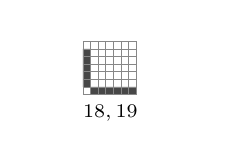
\begin{tikzpicture}[x=1mm,y=1mm,baseline=0mm]
\path[use as bounding box] (0,-.7) rectangle (21.5,11.9);
\begin{scope}[shift={(7.0,3.4)},x=0.97mm,y=0.97mm]
\fill[black!72] (0,5) rectangle (1,6) (0,4) rectangle (1,5) (0,3) rectangle (1,4) (0,2) rectangle (1,3) (0,1) rectangle (1,2) (1,0) rectangle (2,1) (2,0) rectangle (3,1) (3,0) rectangle (4,1) (4,0) rectangle (5,1) (5,0) rectangle (6,1) (6,0) rectangle (7,1);
\draw[black!47,line width=.16pt] (0,0)--(0,7) (0,0)--(7,0) (1,0)--(1,7) (0,1)--(7,1) (2,0)--(2,7) (0,2)--(7,2) (3,0)--(3,7) (0,3)--(7,3) (4,0)--(4,7) (0,4)--(7,4) (5,0)--(5,7) (0,5)--(7,5) (6,0)--(6,7) (0,6)--(7,6) (7,0)--(7,7) (0,7)--(7,7);
\end{scope}
\node[inner sep=0pt,font=\scriptsize] at (10.5,1.1) {$18,19$};
\end{tikzpicture} &
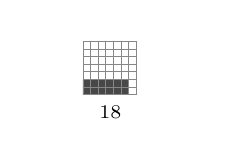
\begin{tikzpicture}[x=1mm,y=1mm,baseline=0mm]
\path[use as bounding box] (0,-.7) rectangle (21.5,11.9);
\begin{scope}[shift={(7.0,3.4)},x=0.97mm,y=0.97mm]
\fill[black!72] (0,1) rectangle (1,2) (1,1) rectangle (2,2) (2,1) rectangle (3,2) (3,1) rectangle (4,2) (4,1) rectangle (5,2) (5,1) rectangle (6,2) (0,0) rectangle (1,1) (1,0) rectangle (2,1) (2,0) rectangle (3,1) (3,0) rectangle (4,1) (4,0) rectangle (5,1) (5,0) rectangle (6,1);
\draw[black!47,line width=.16pt] (0,0)--(0,7) (0,0)--(7,0) (1,0)--(1,7) (0,1)--(7,1) (2,0)--(2,7) (0,2)--(7,2) (3,0)--(3,7) (0,3)--(7,3) (4,0)--(4,7) (0,4)--(7,4) (5,0)--(5,7) (0,5)--(7,5) (6,0)--(6,7) (0,6)--(7,6) (7,0)--(7,7) (0,7)--(7,7);
\end{scope}
\node[inner sep=0pt,font=\scriptsize] at (10.5,1.1) {$18$};
\end{tikzpicture} &
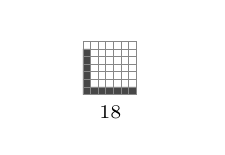
\begin{tikzpicture}[x=1mm,y=1mm,baseline=0mm]
\path[use as bounding box] (0,-.7) rectangle (21.5,11.9);
\begin{scope}[shift={(7.0,3.4)},x=0.97mm,y=0.97mm]
\fill[black!72] (0,5) rectangle (1,6) (0,4) rectangle (1,5) (0,3) rectangle (1,4) (0,2) rectangle (1,3) (0,1) rectangle (1,2) (0,0) rectangle (1,1) (1,0) rectangle (2,1) (2,0) rectangle (3,1) (3,0) rectangle (4,1) (4,0) rectangle (5,1) (5,0) rectangle (6,1) (6,0) rectangle (7,1);
\draw[black!47,line width=.16pt] (0,0)--(0,7) (0,0)--(7,0) (1,0)--(1,7) (0,1)--(7,1) (2,0)--(2,7) (0,2)--(7,2) (3,0)--(3,7) (0,3)--(7,3) (4,0)--(4,7) (0,4)--(7,4) (5,0)--(5,7) (0,5)--(7,5) (6,0)--(6,7) (0,6)--(7,6) (7,0)--(7,7) (0,7)--(7,7);
\end{scope}
\node[inner sep=0pt,font=\scriptsize] at (10.5,1.1) {$18$};
\end{tikzpicture} &
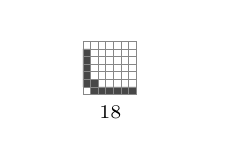
\begin{tikzpicture}[x=1mm,y=1mm,baseline=0mm]
\path[use as bounding box] (0,-.7) rectangle (21.5,11.9);
\begin{scope}[shift={(7.0,3.4)},x=0.97mm,y=0.97mm]
\fill[black!72] (0,5) rectangle (1,6) (0,4) rectangle (1,5) (0,3) rectangle (1,4) (0,2) rectangle (1,3) (0,1) rectangle (1,2) (1,1) rectangle (2,2) (1,0) rectangle (2,1) (2,0) rectangle (3,1) (3,0) rectangle (4,1) (4,0) rectangle (5,1) (5,0) rectangle (6,1) (6,0) rectangle (7,1);
\draw[black!47,line width=.16pt] (0,0)--(0,7) (0,0)--(7,0) (1,0)--(1,7) (0,1)--(7,1) (2,0)--(2,7) (0,2)--(7,2) (3,0)--(3,7) (0,3)--(7,3) (4,0)--(4,7) (0,4)--(7,4) (5,0)--(5,7) (0,5)--(7,5) (6,0)--(6,7) (0,6)--(7,6) (7,0)--(7,7) (0,7)--(7,7);
\end{scope}
\node[inner sep=0pt,font=\scriptsize] at (10.5,1.1) {$18$};
\end{tikzpicture} &
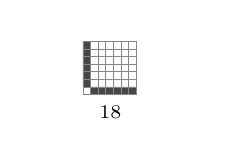
\begin{tikzpicture}[x=1mm,y=1mm,baseline=0mm]
\path[use as bounding box] (0,-.7) rectangle (21.5,11.9);
\begin{scope}[shift={(7.0,3.4)},x=0.97mm,y=0.97mm]
\fill[black!72] (0,6) rectangle (1,7) (0,5) rectangle (1,6) (0,4) rectangle (1,5) (0,3) rectangle (1,4) (0,2) rectangle (1,3) (0,1) rectangle (1,2) (1,0) rectangle (2,1) (2,0) rectangle (3,1) (3,0) rectangle (4,1) (4,0) rectangle (5,1) (5,0) rectangle (6,1) (6,0) rectangle (7,1);
\draw[black!47,line width=.16pt] (0,0)--(0,7) (0,0)--(7,0) (1,0)--(1,7) (0,1)--(7,1) (2,0)--(2,7) (0,2)--(7,2) (3,0)--(3,7) (0,3)--(7,3) (4,0)--(4,7) (0,4)--(7,4) (5,0)--(5,7) (0,5)--(7,5) (6,0)--(6,7) (0,6)--(7,6) (7,0)--(7,7) (0,7)--(7,7);
\end{scope}
\node[inner sep=0pt,font=\scriptsize] at (10.5,1.1) {$18$};
\end{tikzpicture} \\[.4mm]
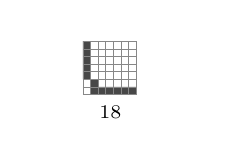
\begin{tikzpicture}[x=1mm,y=1mm,baseline=0mm]
\path[use as bounding box] (0,-.7) rectangle (21.5,11.9);
\begin{scope}[shift={(7.0,3.4)},x=0.97mm,y=0.97mm]
\fill[black!72] (0,6) rectangle (1,7) (0,5) rectangle (1,6) (0,4) rectangle (1,5) (0,3) rectangle (1,4) (0,2) rectangle (1,3) (1,1) rectangle (2,2) (1,0) rectangle (2,1) (2,0) rectangle (3,1) (3,0) rectangle (4,1) (4,0) rectangle (5,1) (5,0) rectangle (6,1) (6,0) rectangle (7,1);
\draw[black!47,line width=.16pt] (0,0)--(0,7) (0,0)--(7,0) (1,0)--(1,7) (0,1)--(7,1) (2,0)--(2,7) (0,2)--(7,2) (3,0)--(3,7) (0,3)--(7,3) (4,0)--(4,7) (0,4)--(7,4) (5,0)--(5,7) (0,5)--(7,5) (6,0)--(6,7) (0,6)--(7,6) (7,0)--(7,7) (0,7)--(7,7);
\end{scope}
\node[inner sep=0pt,font=\scriptsize] at (10.5,1.1) {$18$};
\end{tikzpicture} &
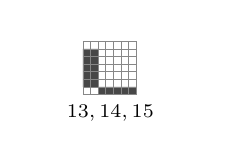
\begin{tikzpicture}[x=1mm,y=1mm,baseline=0mm]
\path[use as bounding box] (0,-.7) rectangle (21.5,11.9);
\begin{scope}[shift={(7.0,3.4)},x=0.97mm,y=0.97mm]
\fill[black!72] (0,5) rectangle (1,6) (1,5) rectangle (2,6) (0,4) rectangle (1,5) (1,4) rectangle (2,5) (0,3) rectangle (1,4) (1,3) rectangle (2,4) (0,2) rectangle (1,3) (1,2) rectangle (2,3) (0,1) rectangle (1,2) (1,1) rectangle (2,2) (2,0) rectangle (3,1) (3,0) rectangle (4,1) (4,0) rectangle (5,1) (5,0) rectangle (6,1) (6,0) rectangle (7,1);
\draw[black!47,line width=.16pt] (0,0)--(0,7) (0,0)--(7,0) (1,0)--(1,7) (0,1)--(7,1) (2,0)--(2,7) (0,2)--(7,2) (3,0)--(3,7) (0,3)--(7,3) (4,0)--(4,7) (0,4)--(7,4) (5,0)--(5,7) (0,5)--(7,5) (6,0)--(6,7) (0,6)--(7,6) (7,0)--(7,7) (0,7)--(7,7);
\end{scope}
\node[inner sep=0pt,font=\scriptsize] at (10.5,1.1) {$13,14,15$};
\end{tikzpicture} &
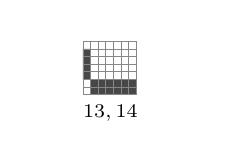
\begin{tikzpicture}[x=1mm,y=1mm,baseline=0mm]
\path[use as bounding box] (0,-.7) rectangle (21.5,11.9);
\begin{scope}[shift={(7.0,3.4)},x=0.97mm,y=0.97mm]
\fill[black!72] (0,5) rectangle (1,6) (0,4) rectangle (1,5) (0,3) rectangle (1,4) (0,2) rectangle (1,3) (1,1) rectangle (2,2) (2,1) rectangle (3,2) (3,1) rectangle (4,2) (4,1) rectangle (5,2) (5,1) rectangle (6,2) (6,1) rectangle (7,2) (1,0) rectangle (2,1) (2,0) rectangle (3,1) (3,0) rectangle (4,1) (4,0) rectangle (5,1) (5,0) rectangle (6,1) (6,0) rectangle (7,1);
\draw[black!47,line width=.16pt] (0,0)--(0,7) (0,0)--(7,0) (1,0)--(1,7) (0,1)--(7,1) (2,0)--(2,7) (0,2)--(7,2) (3,0)--(3,7) (0,3)--(7,3) (4,0)--(4,7) (0,4)--(7,4) (5,0)--(5,7) (0,5)--(7,5) (6,0)--(6,7) (0,6)--(7,6) (7,0)--(7,7) (0,7)--(7,7);
\end{scope}
\node[inner sep=0pt,font=\scriptsize] at (10.5,1.1) {$13,14$};
\end{tikzpicture} &
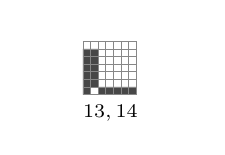
\begin{tikzpicture}[x=1mm,y=1mm,baseline=0mm]
\path[use as bounding box] (0,-.7) rectangle (21.5,11.9);
\begin{scope}[shift={(7.0,3.4)},x=0.97mm,y=0.97mm]
\fill[black!72] (0,5) rectangle (1,6) (1,5) rectangle (2,6) (0,4) rectangle (1,5) (1,4) rectangle (2,5) (0,3) rectangle (1,4) (1,3) rectangle (2,4) (0,2) rectangle (1,3) (1,2) rectangle (2,3) (0,1) rectangle (1,2) (1,1) rectangle (2,2) (0,0) rectangle (1,1) (2,0) rectangle (3,1) (3,0) rectangle (4,1) (4,0) rectangle (5,1) (5,0) rectangle (6,1) (6,0) rectangle (7,1);
\draw[black!47,line width=.16pt] (0,0)--(0,7) (0,0)--(7,0) (1,0)--(1,7) (0,1)--(7,1) (2,0)--(2,7) (0,2)--(7,2) (3,0)--(3,7) (0,3)--(7,3) (4,0)--(4,7) (0,4)--(7,4) (5,0)--(5,7) (0,5)--(7,5) (6,0)--(6,7) (0,6)--(7,6) (7,0)--(7,7) (0,7)--(7,7);
\end{scope}
\node[inner sep=0pt,font=\scriptsize] at (10.5,1.1) {$13,14$};
\end{tikzpicture} &
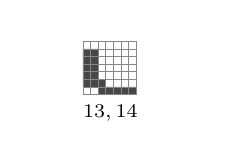
\begin{tikzpicture}[x=1mm,y=1mm,baseline=0mm]
\path[use as bounding box] (0,-.7) rectangle (21.5,11.9);
\begin{scope}[shift={(7.0,3.4)},x=0.97mm,y=0.97mm]
\fill[black!72] (0,5) rectangle (1,6) (1,5) rectangle (2,6) (0,4) rectangle (1,5) (1,4) rectangle (2,5) (0,3) rectangle (1,4) (1,3) rectangle (2,4) (0,2) rectangle (1,3) (1,2) rectangle (2,3) (0,1) rectangle (1,2) (1,1) rectangle (2,2) (2,1) rectangle (3,2) (2,0) rectangle (3,1) (3,0) rectangle (4,1) (4,0) rectangle (5,1) (5,0) rectangle (6,1) (6,0) rectangle (7,1);
\draw[black!47,line width=.16pt] (0,0)--(0,7) (0,0)--(7,0) (1,0)--(1,7) (0,1)--(7,1) (2,0)--(2,7) (0,2)--(7,2) (3,0)--(3,7) (0,3)--(7,3) (4,0)--(4,7) (0,4)--(7,4) (5,0)--(5,7) (0,5)--(7,5) (6,0)--(6,7) (0,6)--(7,6) (7,0)--(7,7) (0,7)--(7,7);
\end{scope}
\node[inner sep=0pt,font=\scriptsize] at (10.5,1.1) {$13,14$};
\end{tikzpicture} \\[.4mm]
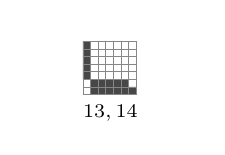
\begin{tikzpicture}[x=1mm,y=1mm,baseline=0mm]
\path[use as bounding box] (0,-.7) rectangle (21.5,11.9);
\begin{scope}[shift={(7.0,3.4)},x=0.97mm,y=0.97mm]
\fill[black!72] (0,6) rectangle (1,7) (0,5) rectangle (1,6) (0,4) rectangle (1,5) (0,3) rectangle (1,4) (0,2) rectangle (1,3) (1,1) rectangle (2,2) (2,1) rectangle (3,2) (3,1) rectangle (4,2) (4,1) rectangle (5,2) (5,1) rectangle (6,2) (1,0) rectangle (2,1) (2,0) rectangle (3,1) (3,0) rectangle (4,1) (4,0) rectangle (5,1) (5,0) rectangle (6,1) (6,0) rectangle (7,1);
\draw[black!47,line width=.16pt] (0,0)--(0,7) (0,0)--(7,0) (1,0)--(1,7) (0,1)--(7,1) (2,0)--(2,7) (0,2)--(7,2) (3,0)--(3,7) (0,3)--(7,3) (4,0)--(4,7) (0,4)--(7,4) (5,0)--(5,7) (0,5)--(7,5) (6,0)--(6,7) (0,6)--(7,6) (7,0)--(7,7) (0,7)--(7,7);
\end{scope}
\node[inner sep=0pt,font=\scriptsize] at (10.5,1.1) {$13,14$};
\end{tikzpicture} &
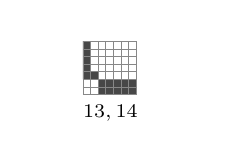
\begin{tikzpicture}[x=1mm,y=1mm,baseline=0mm]
\path[use as bounding box] (0,-.7) rectangle (21.5,11.9);
\begin{scope}[shift={(7.0,3.4)},x=0.97mm,y=0.97mm]
\fill[black!72] (0,6) rectangle (1,7) (0,5) rectangle (1,6) (0,4) rectangle (1,5) (0,3) rectangle (1,4) (0,2) rectangle (1,3) (1,2) rectangle (2,3) (2,1) rectangle (3,2) (3,1) rectangle (4,2) (4,1) rectangle (5,2) (5,1) rectangle (6,2) (6,1) rectangle (7,2) (2,0) rectangle (3,1) (3,0) rectangle (4,1) (4,0) rectangle (5,1) (5,0) rectangle (6,1) (6,0) rectangle (7,1);
\draw[black!47,line width=.16pt] (0,0)--(0,7) (0,0)--(7,0) (1,0)--(1,7) (0,1)--(7,1) (2,0)--(2,7) (0,2)--(7,2) (3,0)--(3,7) (0,3)--(7,3) (4,0)--(4,7) (0,4)--(7,4) (5,0)--(5,7) (0,5)--(7,5) (6,0)--(6,7) (0,6)--(7,6) (7,0)--(7,7) (0,7)--(7,7);
\end{scope}
\node[inner sep=0pt,font=\scriptsize] at (10.5,1.1) {$13,14$};
\end{tikzpicture} &
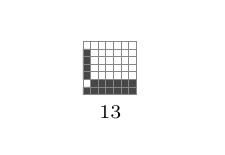
\begin{tikzpicture}[x=1mm,y=1mm,baseline=0mm]
\path[use as bounding box] (0,-.7) rectangle (21.5,11.9);
\begin{scope}[shift={(7.0,3.4)},x=0.97mm,y=0.97mm]
\fill[black!72] (0,5) rectangle (1,6) (0,4) rectangle (1,5) (0,3) rectangle (1,4) (0,2) rectangle (1,3) (1,1) rectangle (2,2) (2,1) rectangle (3,2) (3,1) rectangle (4,2) (4,1) rectangle (5,2) (5,1) rectangle (6,2) (6,1) rectangle (7,2) (0,0) rectangle (1,1) (1,0) rectangle (2,1) (2,0) rectangle (3,1) (3,0) rectangle (4,1) (4,0) rectangle (5,1) (5,0) rectangle (6,1) (6,0) rectangle (7,1);
\draw[black!47,line width=.16pt] (0,0)--(0,7) (0,0)--(7,0) (1,0)--(1,7) (0,1)--(7,1) (2,0)--(2,7) (0,2)--(7,2) (3,0)--(3,7) (0,3)--(7,3) (4,0)--(4,7) (0,4)--(7,4) (5,0)--(5,7) (0,5)--(7,5) (6,0)--(6,7) (0,6)--(7,6) (7,0)--(7,7) (0,7)--(7,7);
\end{scope}
\node[inner sep=0pt,font=\scriptsize] at (10.5,1.1) {$13$};
\end{tikzpicture} &
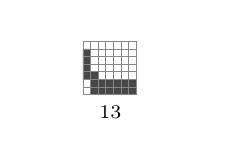
\begin{tikzpicture}[x=1mm,y=1mm,baseline=0mm]
\path[use as bounding box] (0,-.7) rectangle (21.5,11.9);
\begin{scope}[shift={(7.0,3.4)},x=0.97mm,y=0.97mm]
\fill[black!72] (0,5) rectangle (1,6) (0,4) rectangle (1,5) (0,3) rectangle (1,4) (0,2) rectangle (1,3) (1,2) rectangle (2,3) (1,1) rectangle (2,2) (2,1) rectangle (3,2) (3,1) rectangle (4,2) (4,1) rectangle (5,2) (5,1) rectangle (6,2) (6,1) rectangle (7,2) (1,0) rectangle (2,1) (2,0) rectangle (3,1) (3,0) rectangle (4,1) (4,0) rectangle (5,1) (5,0) rectangle (6,1) (6,0) rectangle (7,1);
\draw[black!47,line width=.16pt] (0,0)--(0,7) (0,0)--(7,0) (1,0)--(1,7) (0,1)--(7,1) (2,0)--(2,7) (0,2)--(7,2) (3,0)--(3,7) (0,3)--(7,3) (4,0)--(4,7) (0,4)--(7,4) (5,0)--(5,7) (0,5)--(7,5) (6,0)--(6,7) (0,6)--(7,6) (7,0)--(7,7) (0,7)--(7,7);
\end{scope}
\node[inner sep=0pt,font=\scriptsize] at (10.5,1.1) {$13$};
\end{tikzpicture} &
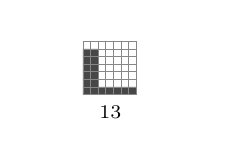
\begin{tikzpicture}[x=1mm,y=1mm,baseline=0mm]
\path[use as bounding box] (0,-.7) rectangle (21.5,11.9);
\begin{scope}[shift={(7.0,3.4)},x=0.97mm,y=0.97mm]
\fill[black!72] (0,5) rectangle (1,6) (1,5) rectangle (2,6) (0,4) rectangle (1,5) (1,4) rectangle (2,5) (0,3) rectangle (1,4) (1,3) rectangle (2,4) (0,2) rectangle (1,3) (1,2) rectangle (2,3) (0,1) rectangle (1,2) (1,1) rectangle (2,2) (0,0) rectangle (1,1) (1,0) rectangle (2,1) (2,0) rectangle (3,1) (3,0) rectangle (4,1) (4,0) rectangle (5,1) (5,0) rectangle (6,1) (6,0) rectangle (7,1);
\draw[black!47,line width=.16pt] (0,0)--(0,7) (0,0)--(7,0) (1,0)--(1,7) (0,1)--(7,1) (2,0)--(2,7) (0,2)--(7,2) (3,0)--(3,7) (0,3)--(7,3) (4,0)--(4,7) (0,4)--(7,4) (5,0)--(5,7) (0,5)--(7,5) (6,0)--(6,7) (0,6)--(7,6) (7,0)--(7,7) (0,7)--(7,7);
\end{scope}
\node[inner sep=0pt,font=\scriptsize] at (10.5,1.1) {$13$};
\end{tikzpicture} \\[.4mm]
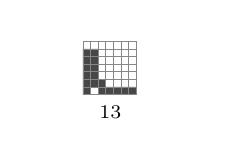
\begin{tikzpicture}[x=1mm,y=1mm,baseline=0mm]
\path[use as bounding box] (0,-.7) rectangle (21.5,11.9);
\begin{scope}[shift={(7.0,3.4)},x=0.97mm,y=0.97mm]
\fill[black!72] (0,5) rectangle (1,6) (1,5) rectangle (2,6) (0,4) rectangle (1,5) (1,4) rectangle (2,5) (0,3) rectangle (1,4) (1,3) rectangle (2,4) (0,2) rectangle (1,3) (1,2) rectangle (2,3) (0,1) rectangle (1,2) (1,1) rectangle (2,2) (2,1) rectangle (3,2) (0,0) rectangle (1,1) (2,0) rectangle (3,1) (3,0) rectangle (4,1) (4,0) rectangle (5,1) (5,0) rectangle (6,1) (6,0) rectangle (7,1);
\draw[black!47,line width=.16pt] (0,0)--(0,7) (0,0)--(7,0) (1,0)--(1,7) (0,1)--(7,1) (2,0)--(2,7) (0,2)--(7,2) (3,0)--(3,7) (0,3)--(7,3) (4,0)--(4,7) (0,4)--(7,4) (5,0)--(5,7) (0,5)--(7,5) (6,0)--(6,7) (0,6)--(7,6) (7,0)--(7,7) (0,7)--(7,7);
\end{scope}
\node[inner sep=0pt,font=\scriptsize] at (10.5,1.1) {$13$};
\end{tikzpicture} &
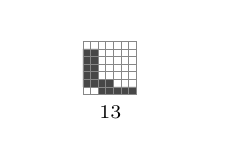
\begin{tikzpicture}[x=1mm,y=1mm,baseline=0mm]
\path[use as bounding box] (0,-.7) rectangle (21.5,11.9);
\begin{scope}[shift={(7.0,3.4)},x=0.97mm,y=0.97mm]
\fill[black!72] (0,5) rectangle (1,6) (1,5) rectangle (2,6) (0,4) rectangle (1,5) (1,4) rectangle (2,5) (0,3) rectangle (1,4) (1,3) rectangle (2,4) (0,2) rectangle (1,3) (1,2) rectangle (2,3) (0,1) rectangle (1,2) (1,1) rectangle (2,2) (2,1) rectangle (3,2) (3,1) rectangle (4,2) (2,0) rectangle (3,1) (3,0) rectangle (4,1) (4,0) rectangle (5,1) (5,0) rectangle (6,1) (6,0) rectangle (7,1);
\draw[black!47,line width=.16pt] (0,0)--(0,7) (0,0)--(7,0) (1,0)--(1,7) (0,1)--(7,1) (2,0)--(2,7) (0,2)--(7,2) (3,0)--(3,7) (0,3)--(7,3) (4,0)--(4,7) (0,4)--(7,4) (5,0)--(5,7) (0,5)--(7,5) (6,0)--(6,7) (0,6)--(7,6) (7,0)--(7,7) (0,7)--(7,7);
\end{scope}
\node[inner sep=0pt,font=\scriptsize] at (10.5,1.1) {$13$};
\end{tikzpicture} &
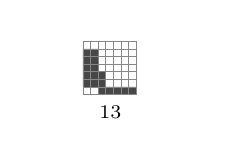
\begin{tikzpicture}[x=1mm,y=1mm,baseline=0mm]
\path[use as bounding box] (0,-.7) rectangle (21.5,11.9);
\begin{scope}[shift={(7.0,3.4)},x=0.97mm,y=0.97mm]
\fill[black!72] (0,5) rectangle (1,6) (1,5) rectangle (2,6) (0,4) rectangle (1,5) (1,4) rectangle (2,5) (0,3) rectangle (1,4) (1,3) rectangle (2,4) (0,2) rectangle (1,3) (1,2) rectangle (2,3) (2,2) rectangle (3,3) (0,1) rectangle (1,2) (1,1) rectangle (2,2) (2,1) rectangle (3,2) (2,0) rectangle (3,1) (3,0) rectangle (4,1) (4,0) rectangle (5,1) (5,0) rectangle (6,1) (6,0) rectangle (7,1);
\draw[black!47,line width=.16pt] (0,0)--(0,7) (0,0)--(7,0) (1,0)--(1,7) (0,1)--(7,1) (2,0)--(2,7) (0,2)--(7,2) (3,0)--(3,7) (0,3)--(7,3) (4,0)--(4,7) (0,4)--(7,4) (5,0)--(5,7) (0,5)--(7,5) (6,0)--(6,7) (0,6)--(7,6) (7,0)--(7,7) (0,7)--(7,7);
\end{scope}
\node[inner sep=0pt,font=\scriptsize] at (10.5,1.1) {$13$};
\end{tikzpicture} &
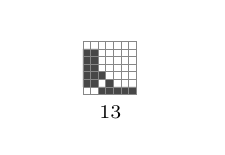
\begin{tikzpicture}[x=1mm,y=1mm,baseline=0mm]
\path[use as bounding box] (0,-.7) rectangle (21.5,11.9);
\begin{scope}[shift={(7.0,3.4)},x=0.97mm,y=0.97mm]
\fill[black!72] (0,5) rectangle (1,6) (1,5) rectangle (2,6) (0,4) rectangle (1,5) (1,4) rectangle (2,5) (0,3) rectangle (1,4) (1,3) rectangle (2,4) (0,2) rectangle (1,3) (1,2) rectangle (2,3) (2,2) rectangle (3,3) (0,1) rectangle (1,2) (1,1) rectangle (2,2) (3,1) rectangle (4,2) (2,0) rectangle (3,1) (3,0) rectangle (4,1) (4,0) rectangle (5,1) (5,0) rectangle (6,1) (6,0) rectangle (7,1);
\draw[black!47,line width=.16pt] (0,0)--(0,7) (0,0)--(7,0) (1,0)--(1,7) (0,1)--(7,1) (2,0)--(2,7) (0,2)--(7,2) (3,0)--(3,7) (0,3)--(7,3) (4,0)--(4,7) (0,4)--(7,4) (5,0)--(5,7) (0,5)--(7,5) (6,0)--(6,7) (0,6)--(7,6) (7,0)--(7,7) (0,7)--(7,7);
\end{scope}
\node[inner sep=0pt,font=\scriptsize] at (10.5,1.1) {$13$};
\end{tikzpicture} &
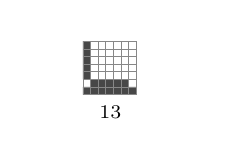
\begin{tikzpicture}[x=1mm,y=1mm,baseline=0mm]
\path[use as bounding box] (0,-.7) rectangle (21.5,11.9);
\begin{scope}[shift={(7.0,3.4)},x=0.97mm,y=0.97mm]
\fill[black!72] (0,6) rectangle (1,7) (0,5) rectangle (1,6) (0,4) rectangle (1,5) (0,3) rectangle (1,4) (0,2) rectangle (1,3) (1,1) rectangle (2,2) (2,1) rectangle (3,2) (3,1) rectangle (4,2) (4,1) rectangle (5,2) (5,1) rectangle (6,2) (0,0) rectangle (1,1) (1,0) rectangle (2,1) (2,0) rectangle (3,1) (3,0) rectangle (4,1) (4,0) rectangle (5,1) (5,0) rectangle (6,1) (6,0) rectangle (7,1);
\draw[black!47,line width=.16pt] (0,0)--(0,7) (0,0)--(7,0) (1,0)--(1,7) (0,1)--(7,1) (2,0)--(2,7) (0,2)--(7,2) (3,0)--(3,7) (0,3)--(7,3) (4,0)--(4,7) (0,4)--(7,4) (5,0)--(5,7) (0,5)--(7,5) (6,0)--(6,7) (0,6)--(7,6) (7,0)--(7,7) (0,7)--(7,7);
\end{scope}
\node[inner sep=0pt,font=\scriptsize] at (10.5,1.1) {$13$};
\end{tikzpicture} \\[.4mm]
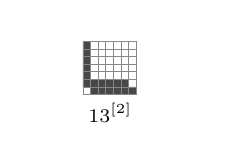
\begin{tikzpicture}[x=1mm,y=1mm,baseline=0mm]
\path[use as bounding box] (0,-.7) rectangle (21.5,11.9);
\begin{scope}[shift={(7.0,3.4)},x=0.97mm,y=0.97mm]
\fill[black!72] (0,6) rectangle (1,7) (0,5) rectangle (1,6) (0,4) rectangle (1,5) (0,3) rectangle (1,4) (0,2) rectangle (1,3) (0,1) rectangle (1,2) (1,1) rectangle (2,2) (2,1) rectangle (3,2) (3,1) rectangle (4,2) (4,1) rectangle (5,2) (5,1) rectangle (6,2) (1,0) rectangle (2,1) (2,0) rectangle (3,1) (3,0) rectangle (4,1) (4,0) rectangle (5,1) (5,0) rectangle (6,1) (6,0) rectangle (7,1);
\draw[black!47,line width=.16pt] (0,0)--(0,7) (0,0)--(7,0) (1,0)--(1,7) (0,1)--(7,1) (2,0)--(2,7) (0,2)--(7,2) (3,0)--(3,7) (0,3)--(7,3) (4,0)--(4,7) (0,4)--(7,4) (5,0)--(5,7) (0,5)--(7,5) (6,0)--(6,7) (0,6)--(7,6) (7,0)--(7,7) (0,7)--(7,7);
\end{scope}
\node[inner sep=0pt,font=\scriptsize] at (10.5,1.1) {$13^{[2]}$};
\end{tikzpicture} &
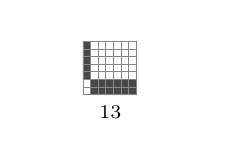
\begin{tikzpicture}[x=1mm,y=1mm,baseline=0mm]
\path[use as bounding box] (0,-.7) rectangle (21.5,11.9);
\begin{scope}[shift={(7.0,3.4)},x=0.97mm,y=0.97mm]
\fill[black!72] (0,6) rectangle (1,7) (0,5) rectangle (1,6) (0,4) rectangle (1,5) (0,3) rectangle (1,4) (0,2) rectangle (1,3) (1,1) rectangle (2,2) (2,1) rectangle (3,2) (3,1) rectangle (4,2) (4,1) rectangle (5,2) (5,1) rectangle (6,2) (6,1) rectangle (7,2) (1,0) rectangle (2,1) (2,0) rectangle (3,1) (3,0) rectangle (4,1) (4,0) rectangle (5,1) (5,0) rectangle (6,1) (6,0) rectangle (7,1);
\draw[black!47,line width=.16pt] (0,0)--(0,7) (0,0)--(7,0) (1,0)--(1,7) (0,1)--(7,1) (2,0)--(2,7) (0,2)--(7,2) (3,0)--(3,7) (0,3)--(7,3) (4,0)--(4,7) (0,4)--(7,4) (5,0)--(5,7) (0,5)--(7,5) (6,0)--(6,7) (0,6)--(7,6) (7,0)--(7,7) (0,7)--(7,7);
\end{scope}
\node[inner sep=0pt,font=\scriptsize] at (10.5,1.1) {$13$};
\end{tikzpicture} &
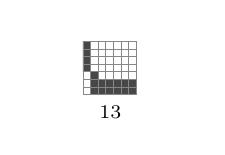
\begin{tikzpicture}[x=1mm,y=1mm,baseline=0mm]
\path[use as bounding box] (0,-.7) rectangle (21.5,11.9);
\begin{scope}[shift={(7.0,3.4)},x=0.97mm,y=0.97mm]
\fill[black!72] (0,6) rectangle (1,7) (0,5) rectangle (1,6) (0,4) rectangle (1,5) (0,3) rectangle (1,4) (1,2) rectangle (2,3) (1,1) rectangle (2,2) (2,1) rectangle (3,2) (3,1) rectangle (4,2) (4,1) rectangle (5,2) (5,1) rectangle (6,2) (6,1) rectangle (7,2) (1,0) rectangle (2,1) (2,0) rectangle (3,1) (3,0) rectangle (4,1) (4,0) rectangle (5,1) (5,0) rectangle (6,1) (6,0) rectangle (7,1);
\draw[black!47,line width=.16pt] (0,0)--(0,7) (0,0)--(7,0) (1,0)--(1,7) (0,1)--(7,1) (2,0)--(2,7) (0,2)--(7,2) (3,0)--(3,7) (0,3)--(7,3) (4,0)--(4,7) (0,4)--(7,4) (5,0)--(5,7) (0,5)--(7,5) (6,0)--(6,7) (0,6)--(7,6) (7,0)--(7,7) (0,7)--(7,7);
\end{scope}
\node[inner sep=0pt,font=\scriptsize] at (10.5,1.1) {$13$};
\end{tikzpicture} &
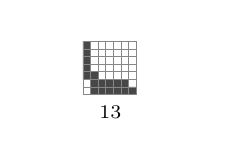
\begin{tikzpicture}[x=1mm,y=1mm,baseline=0mm]
\path[use as bounding box] (0,-.7) rectangle (21.5,11.9);
\begin{scope}[shift={(7.0,3.4)},x=0.97mm,y=0.97mm]
\fill[black!72] (0,6) rectangle (1,7) (0,5) rectangle (1,6) (0,4) rectangle (1,5) (0,3) rectangle (1,4) (0,2) rectangle (1,3) (1,2) rectangle (2,3) (1,1) rectangle (2,2) (2,1) rectangle (3,2) (3,1) rectangle (4,2) (4,1) rectangle (5,2) (5,1) rectangle (6,2) (1,0) rectangle (2,1) (2,0) rectangle (3,1) (3,0) rectangle (4,1) (4,0) rectangle (5,1) (5,0) rectangle (6,1) (6,0) rectangle (7,1);
\draw[black!47,line width=.16pt] (0,0)--(0,7) (0,0)--(7,0) (1,0)--(1,7) (0,1)--(7,1) (2,0)--(2,7) (0,2)--(7,2) (3,0)--(3,7) (0,3)--(7,3) (4,0)--(4,7) (0,4)--(7,4) (5,0)--(5,7) (0,5)--(7,5) (6,0)--(6,7) (0,6)--(7,6) (7,0)--(7,7) (0,7)--(7,7);
\end{scope}
\node[inner sep=0pt,font=\scriptsize] at (10.5,1.1) {$13$};
\end{tikzpicture} &
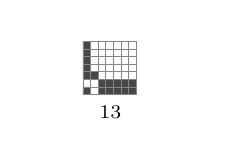
\begin{tikzpicture}[x=1mm,y=1mm,baseline=0mm]
\path[use as bounding box] (0,-.7) rectangle (21.5,11.9);
\begin{scope}[shift={(7.0,3.4)},x=0.97mm,y=0.97mm]
\fill[black!72] (0,6) rectangle (1,7) (0,5) rectangle (1,6) (0,4) rectangle (1,5) (0,3) rectangle (1,4) (0,2) rectangle (1,3) (1,2) rectangle (2,3) (2,1) rectangle (3,2) (3,1) rectangle (4,2) (4,1) rectangle (5,2) (5,1) rectangle (6,2) (6,1) rectangle (7,2) (0,0) rectangle (1,1) (2,0) rectangle (3,1) (3,0) rectangle (4,1) (4,0) rectangle (5,1) (5,0) rectangle (6,1) (6,0) rectangle (7,1);
\draw[black!47,line width=.16pt] (0,0)--(0,7) (0,0)--(7,0) (1,0)--(1,7) (0,1)--(7,1) (2,0)--(2,7) (0,2)--(7,2) (3,0)--(3,7) (0,3)--(7,3) (4,0)--(4,7) (0,4)--(7,4) (5,0)--(5,7) (0,5)--(7,5) (6,0)--(6,7) (0,6)--(7,6) (7,0)--(7,7) (0,7)--(7,7);
\end{scope}
\node[inner sep=0pt,font=\scriptsize] at (10.5,1.1) {$13$};
\end{tikzpicture} \\[.4mm]
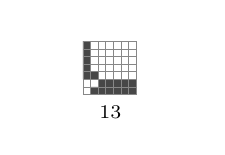
\begin{tikzpicture}[x=1mm,y=1mm,baseline=0mm]
\path[use as bounding box] (0,-.7) rectangle (21.5,11.9);
\begin{scope}[shift={(7.0,3.4)},x=0.97mm,y=0.97mm]
\fill[black!72] (0,6) rectangle (1,7) (0,5) rectangle (1,6) (0,4) rectangle (1,5) (0,3) rectangle (1,4) (0,2) rectangle (1,3) (1,2) rectangle (2,3) (2,1) rectangle (3,2) (3,1) rectangle (4,2) (4,1) rectangle (5,2) (5,1) rectangle (6,2) (6,1) rectangle (7,2) (1,0) rectangle (2,1) (2,0) rectangle (3,1) (3,0) rectangle (4,1) (4,0) rectangle (5,1) (5,0) rectangle (6,1) (6,0) rectangle (7,1);
\draw[black!47,line width=.16pt] (0,0)--(0,7) (0,0)--(7,0) (1,0)--(1,7) (0,1)--(7,1) (2,0)--(2,7) (0,2)--(7,2) (3,0)--(3,7) (0,3)--(7,3) (4,0)--(4,7) (0,4)--(7,4) (5,0)--(5,7) (0,5)--(7,5) (6,0)--(6,7) (0,6)--(7,6) (7,0)--(7,7) (0,7)--(7,7);
\end{scope}
\node[inner sep=0pt,font=\scriptsize] at (10.5,1.1) {$13$};
\end{tikzpicture} &
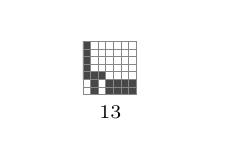
\begin{tikzpicture}[x=1mm,y=1mm,baseline=0mm]
\path[use as bounding box] (0,-.7) rectangle (21.5,11.9);
\begin{scope}[shift={(7.0,3.4)},x=0.97mm,y=0.97mm]
\fill[black!72] (0,6) rectangle (1,7) (0,5) rectangle (1,6) (0,4) rectangle (1,5) (0,3) rectangle (1,4) (0,2) rectangle (1,3) (1,2) rectangle (2,3) (2,2) rectangle (3,3) (1,1) rectangle (2,2) (3,1) rectangle (4,2) (4,1) rectangle (5,2) (5,1) rectangle (6,2) (6,1) rectangle (7,2) (1,0) rectangle (2,1) (3,0) rectangle (4,1) (4,0) rectangle (5,1) (5,0) rectangle (6,1) (6,0) rectangle (7,1);
\draw[black!47,line width=.16pt] (0,0)--(0,7) (0,0)--(7,0) (1,0)--(1,7) (0,1)--(7,1) (2,0)--(2,7) (0,2)--(7,2) (3,0)--(3,7) (0,3)--(7,3) (4,0)--(4,7) (0,4)--(7,4) (5,0)--(5,7) (0,5)--(7,5) (6,0)--(6,7) (0,6)--(7,6) (7,0)--(7,7) (0,7)--(7,7);
\end{scope}
\node[inner sep=0pt,font=\scriptsize] at (10.5,1.1) {$13$};
\end{tikzpicture} &
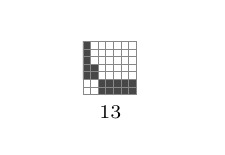
\begin{tikzpicture}[x=1mm,y=1mm,baseline=0mm]
\path[use as bounding box] (0,-.7) rectangle (21.5,11.9);
\begin{scope}[shift={(7.0,3.4)},x=0.97mm,y=0.97mm]
\fill[black!72] (0,6) rectangle (1,7) (0,5) rectangle (1,6) (0,4) rectangle (1,5) (0,3) rectangle (1,4) (1,3) rectangle (2,4) (0,2) rectangle (1,3) (1,2) rectangle (2,3) (2,1) rectangle (3,2) (3,1) rectangle (4,2) (4,1) rectangle (5,2) (5,1) rectangle (6,2) (6,1) rectangle (7,2) (2,0) rectangle (3,1) (3,0) rectangle (4,1) (4,0) rectangle (5,1) (5,0) rectangle (6,1) (6,0) rectangle (7,1);
\draw[black!47,line width=.16pt] (0,0)--(0,7) (0,0)--(7,0) (1,0)--(1,7) (0,1)--(7,1) (2,0)--(2,7) (0,2)--(7,2) (3,0)--(3,7) (0,3)--(7,3) (4,0)--(4,7) (0,4)--(7,4) (5,0)--(5,7) (0,5)--(7,5) (6,0)--(6,7) (0,6)--(7,6) (7,0)--(7,7) (0,7)--(7,7);
\end{scope}
\node[inner sep=0pt,font=\scriptsize] at (10.5,1.1) {$13$};
\end{tikzpicture} &
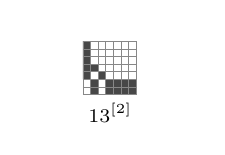
\begin{tikzpicture}[x=1mm,y=1mm,baseline=0mm]
\path[use as bounding box] (0,-.7) rectangle (21.5,11.9);
\begin{scope}[shift={(7.0,3.4)},x=0.97mm,y=0.97mm]
\fill[black!72] (0,6) rectangle (1,7) (0,5) rectangle (1,6) (0,4) rectangle (1,5) (0,3) rectangle (1,4) (1,3) rectangle (2,4) (0,2) rectangle (1,3) (2,2) rectangle (3,3) (1,1) rectangle (2,2) (3,1) rectangle (4,2) (4,1) rectangle (5,2) (5,1) rectangle (6,2) (6,1) rectangle (7,2) (1,0) rectangle (2,1) (3,0) rectangle (4,1) (4,0) rectangle (5,1) (5,0) rectangle (6,1) (6,0) rectangle (7,1);
\draw[black!47,line width=.16pt] (0,0)--(0,7) (0,0)--(7,0) (1,0)--(1,7) (0,1)--(7,1) (2,0)--(2,7) (0,2)--(7,2) (3,0)--(3,7) (0,3)--(7,3) (4,0)--(4,7) (0,4)--(7,4) (5,0)--(5,7) (0,5)--(7,5) (6,0)--(6,7) (0,6)--(7,6) (7,0)--(7,7) (0,7)--(7,7);
\end{scope}
\node[inner sep=0pt,font=\scriptsize] at (10.5,1.1) {$13^{[2]}$};
\end{tikzpicture} &
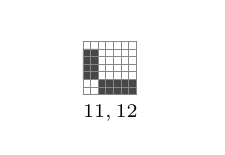
\begin{tikzpicture}[x=1mm,y=1mm,baseline=0mm]
\path[use as bounding box] (0,-.7) rectangle (21.5,11.9);
\begin{scope}[shift={(7.0,3.4)},x=0.97mm,y=0.97mm]
\fill[black!72] (0,5) rectangle (1,6) (1,5) rectangle (2,6) (0,4) rectangle (1,5) (1,4) rectangle (2,5) (0,3) rectangle (1,4) (1,3) rectangle (2,4) (0,2) rectangle (1,3) (1,2) rectangle (2,3) (2,1) rectangle (3,2) (3,1) rectangle (4,2) (4,1) rectangle (5,2) (5,1) rectangle (6,2) (6,1) rectangle (7,2) (2,0) rectangle (3,1) (3,0) rectangle (4,1) (4,0) rectangle (5,1) (5,0) rectangle (6,1) (6,0) rectangle (7,1);
\draw[black!47,line width=.16pt] (0,0)--(0,7) (0,0)--(7,0) (1,0)--(1,7) (0,1)--(7,1) (2,0)--(2,7) (0,2)--(7,2) (3,0)--(3,7) (0,3)--(7,3) (4,0)--(4,7) (0,4)--(7,4) (5,0)--(5,7) (0,5)--(7,5) (6,0)--(6,7) (0,6)--(7,6) (7,0)--(7,7) (0,7)--(7,7);
\end{scope}
\node[inner sep=0pt,font=\scriptsize] at (10.5,1.1) {$11,12$};
\end{tikzpicture} \\[.4mm]
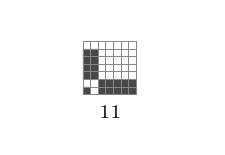
\begin{tikzpicture}[x=1mm,y=1mm,baseline=0mm]
\path[use as bounding box] (0,-.7) rectangle (21.5,11.9);
\begin{scope}[shift={(7.0,3.4)},x=0.97mm,y=0.97mm]
\fill[black!72] (0,5) rectangle (1,6) (1,5) rectangle (2,6) (0,4) rectangle (1,5) (1,4) rectangle (2,5) (0,3) rectangle (1,4) (1,3) rectangle (2,4) (0,2) rectangle (1,3) (1,2) rectangle (2,3) (2,1) rectangle (3,2) (3,1) rectangle (4,2) (4,1) rectangle (5,2) (5,1) rectangle (6,2) (6,1) rectangle (7,2) (0,0) rectangle (1,1) (2,0) rectangle (3,1) (3,0) rectangle (4,1) (4,0) rectangle (5,1) (5,0) rectangle (6,1) (6,0) rectangle (7,1);
\draw[black!47,line width=.16pt] (0,0)--(0,7) (0,0)--(7,0) (1,0)--(1,7) (0,1)--(7,1) (2,0)--(2,7) (0,2)--(7,2) (3,0)--(3,7) (0,3)--(7,3) (4,0)--(4,7) (0,4)--(7,4) (5,0)--(5,7) (0,5)--(7,5) (6,0)--(6,7) (0,6)--(7,6) (7,0)--(7,7) (0,7)--(7,7);
\end{scope}
\node[inner sep=0pt,font=\scriptsize] at (10.5,1.1) {$11$};
\end{tikzpicture} &
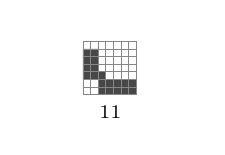
\begin{tikzpicture}[x=1mm,y=1mm,baseline=0mm]
\path[use as bounding box] (0,-.7) rectangle (21.5,11.9);
\begin{scope}[shift={(7.0,3.4)},x=0.97mm,y=0.97mm]
\fill[black!72] (0,5) rectangle (1,6) (1,5) rectangle (2,6) (0,4) rectangle (1,5) (1,4) rectangle (2,5) (0,3) rectangle (1,4) (1,3) rectangle (2,4) (0,2) rectangle (1,3) (1,2) rectangle (2,3) (2,2) rectangle (3,3) (2,1) rectangle (3,2) (3,1) rectangle (4,2) (4,1) rectangle (5,2) (5,1) rectangle (6,2) (6,1) rectangle (7,2) (2,0) rectangle (3,1) (3,0) rectangle (4,1) (4,0) rectangle (5,1) (5,0) rectangle (6,1) (6,0) rectangle (7,1);
\draw[black!47,line width=.16pt] (0,0)--(0,7) (0,0)--(7,0) (1,0)--(1,7) (0,1)--(7,1) (2,0)--(2,7) (0,2)--(7,2) (3,0)--(3,7) (0,3)--(7,3) (4,0)--(4,7) (0,4)--(7,4) (5,0)--(5,7) (0,5)--(7,5) (6,0)--(6,7) (0,6)--(7,6) (7,0)--(7,7) (0,7)--(7,7);
\end{scope}
\node[inner sep=0pt,font=\scriptsize] at (10.5,1.1) {$11$};
\end{tikzpicture} &
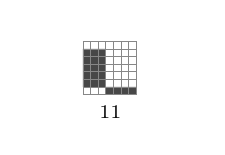
\begin{tikzpicture}[x=1mm,y=1mm,baseline=0mm]
\path[use as bounding box] (0,-.7) rectangle (21.5,11.9);
\begin{scope}[shift={(7.0,3.4)},x=0.97mm,y=0.97mm]
\fill[black!72] (0,5) rectangle (1,6) (1,5) rectangle (2,6) (2,5) rectangle (3,6) (0,4) rectangle (1,5) (1,4) rectangle (2,5) (2,4) rectangle (3,5) (0,3) rectangle (1,4) (1,3) rectangle (2,4) (2,3) rectangle (3,4) (0,2) rectangle (1,3) (1,2) rectangle (2,3) (2,2) rectangle (3,3) (0,1) rectangle (1,2) (1,1) rectangle (2,2) (2,1) rectangle (3,2) (3,0) rectangle (4,1) (4,0) rectangle (5,1) (5,0) rectangle (6,1) (6,0) rectangle (7,1);
\draw[black!47,line width=.16pt] (0,0)--(0,7) (0,0)--(7,0) (1,0)--(1,7) (0,1)--(7,1) (2,0)--(2,7) (0,2)--(7,2) (3,0)--(3,7) (0,3)--(7,3) (4,0)--(4,7) (0,4)--(7,4) (5,0)--(5,7) (0,5)--(7,5) (6,0)--(6,7) (0,6)--(7,6) (7,0)--(7,7) (0,7)--(7,7);
\end{scope}
\node[inner sep=0pt,font=\scriptsize] at (10.5,1.1) {$11$};
\end{tikzpicture} &
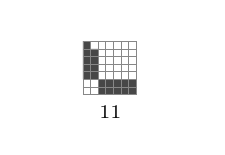
\begin{tikzpicture}[x=1mm,y=1mm,baseline=0mm]
\path[use as bounding box] (0,-.7) rectangle (21.5,11.9);
\begin{scope}[shift={(7.0,3.4)},x=0.97mm,y=0.97mm]
\fill[black!72] (0,6) rectangle (1,7) (0,5) rectangle (1,6) (1,5) rectangle (2,6) (0,4) rectangle (1,5) (1,4) rectangle (2,5) (0,3) rectangle (1,4) (1,3) rectangle (2,4) (0,2) rectangle (1,3) (1,2) rectangle (2,3) (2,1) rectangle (3,2) (3,1) rectangle (4,2) (4,1) rectangle (5,2) (5,1) rectangle (6,2) (6,1) rectangle (7,2) (2,0) rectangle (3,1) (3,0) rectangle (4,1) (4,0) rectangle (5,1) (5,0) rectangle (6,1) (6,0) rectangle (7,1);
\draw[black!47,line width=.16pt] (0,0)--(0,7) (0,0)--(7,0) (1,0)--(1,7) (0,1)--(7,1) (2,0)--(2,7) (0,2)--(7,2) (3,0)--(3,7) (0,3)--(7,3) (4,0)--(4,7) (0,4)--(7,4) (5,0)--(5,7) (0,5)--(7,5) (6,0)--(6,7) (0,6)--(7,6) (7,0)--(7,7) (0,7)--(7,7);
\end{scope}
\node[inner sep=0pt,font=\scriptsize] at (10.5,1.1) {$11$};
\end{tikzpicture} &
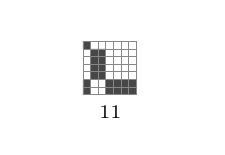
\begin{tikzpicture}[x=1mm,y=1mm,baseline=0mm]
\path[use as bounding box] (0,-.7) rectangle (21.5,11.9);
\begin{scope}[shift={(7.0,3.4)},x=0.97mm,y=0.97mm]
\fill[black!72] (0,6) rectangle (1,7) (1,5) rectangle (2,6) (2,5) rectangle (3,6) (1,4) rectangle (2,5) (2,4) rectangle (3,5) (1,3) rectangle (2,4) (2,3) rectangle (3,4) (1,2) rectangle (2,3) (2,2) rectangle (3,3) (0,1) rectangle (1,2) (3,1) rectangle (4,2) (4,1) rectangle (5,2) (5,1) rectangle (6,2) (6,1) rectangle (7,2) (0,0) rectangle (1,1) (3,0) rectangle (4,1) (4,0) rectangle (5,1) (5,0) rectangle (6,1) (6,0) rectangle (7,1);
\draw[black!47,line width=.16pt] (0,0)--(0,7) (0,0)--(7,0) (1,0)--(1,7) (0,1)--(7,1) (2,0)--(2,7) (0,2)--(7,2) (3,0)--(3,7) (0,3)--(7,3) (4,0)--(4,7) (0,4)--(7,4) (5,0)--(5,7) (0,5)--(7,5) (6,0)--(6,7) (0,6)--(7,6) (7,0)--(7,7) (0,7)--(7,7);
\end{scope}
\node[inner sep=0pt,font=\scriptsize] at (10.5,1.1) {$11$};
\end{tikzpicture} \\[.4mm]
\end{tabular}
\caption{Cross adjacencies tested in the connected case, part 1 of 2.}
\label{fig:nine-qfourteen-connected}
\end{figure}

\begin{figure}[!htbp]
\centering
\begin{tabular}{@{}c@{\hspace{1.6mm}}c@{\hspace{1.6mm}}c@{\hspace{1.6mm}}c@{\hspace{1.6mm}}c@{}}
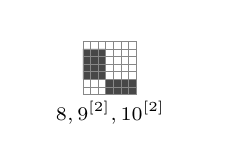
\begin{tikzpicture}[x=1mm,y=1mm,baseline=0mm]
\path[use as bounding box] (0,-.7) rectangle (21.5,11.9);
\begin{scope}[shift={(7.0,3.4)},x=0.97mm,y=0.97mm]
\fill[black!72] (0,5) rectangle (1,6) (1,5) rectangle (2,6) (2,5) rectangle (3,6) (0,4) rectangle (1,5) (1,4) rectangle (2,5) (2,4) rectangle (3,5) (0,3) rectangle (1,4) (1,3) rectangle (2,4) (2,3) rectangle (3,4) (0,2) rectangle (1,3) (1,2) rectangle (2,3) (2,2) rectangle (3,3) (3,1) rectangle (4,2) (4,1) rectangle (5,2) (5,1) rectangle (6,2) (6,1) rectangle (7,2) (3,0) rectangle (4,1) (4,0) rectangle (5,1) (5,0) rectangle (6,1) (6,0) rectangle (7,1);
\draw[black!47,line width=.16pt] (0,0)--(0,7) (0,0)--(7,0) (1,0)--(1,7) (0,1)--(7,1) (2,0)--(2,7) (0,2)--(7,2) (3,0)--(3,7) (0,3)--(7,3) (4,0)--(4,7) (0,4)--(7,4) (5,0)--(5,7) (0,5)--(7,5) (6,0)--(6,7) (0,6)--(7,6) (7,0)--(7,7) (0,7)--(7,7);
\end{scope}
\node[inner sep=0pt,font=\scriptsize] at (10.5,1.1) {$8,9^{[2]},10^{[2]}$};
\end{tikzpicture} &
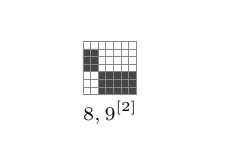
\begin{tikzpicture}[x=1mm,y=1mm,baseline=0mm]
\path[use as bounding box] (0,-.7) rectangle (21.5,11.9);
\begin{scope}[shift={(7.0,3.4)},x=0.97mm,y=0.97mm]
\fill[black!72] (0,5) rectangle (1,6) (1,5) rectangle (2,6) (0,4) rectangle (1,5) (1,4) rectangle (2,5) (0,3) rectangle (1,4) (1,3) rectangle (2,4) (2,2) rectangle (3,3) (3,2) rectangle (4,3) (4,2) rectangle (5,3) (5,2) rectangle (6,3) (6,2) rectangle (7,3) (2,1) rectangle (3,2) (3,1) rectangle (4,2) (4,1) rectangle (5,2) (5,1) rectangle (6,2) (6,1) rectangle (7,2) (2,0) rectangle (3,1) (3,0) rectangle (4,1) (4,0) rectangle (5,1) (5,0) rectangle (6,1) (6,0) rectangle (7,1);
\draw[black!47,line width=.16pt] (0,0)--(0,7) (0,0)--(7,0) (1,0)--(1,7) (0,1)--(7,1) (2,0)--(2,7) (0,2)--(7,2) (3,0)--(3,7) (0,3)--(7,3) (4,0)--(4,7) (0,4)--(7,4) (5,0)--(5,7) (0,5)--(7,5) (6,0)--(6,7) (0,6)--(7,6) (7,0)--(7,7) (0,7)--(7,7);
\end{scope}
\node[inner sep=0pt,font=\scriptsize] at (10.5,1.1) {$8,9^{[2]}$};
\end{tikzpicture} &
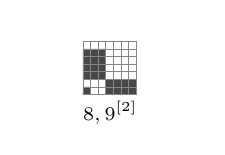
\begin{tikzpicture}[x=1mm,y=1mm,baseline=0mm]
\path[use as bounding box] (0,-.7) rectangle (21.5,11.9);
\begin{scope}[shift={(7.0,3.4)},x=0.97mm,y=0.97mm]
\fill[black!72] (0,5) rectangle (1,6) (1,5) rectangle (2,6) (2,5) rectangle (3,6) (0,4) rectangle (1,5) (1,4) rectangle (2,5) (2,4) rectangle (3,5) (0,3) rectangle (1,4) (1,3) rectangle (2,4) (2,3) rectangle (3,4) (0,2) rectangle (1,3) (1,2) rectangle (2,3) (2,2) rectangle (3,3) (3,1) rectangle (4,2) (4,1) rectangle (5,2) (5,1) rectangle (6,2) (6,1) rectangle (7,2) (0,0) rectangle (1,1) (3,0) rectangle (4,1) (4,0) rectangle (5,1) (5,0) rectangle (6,1) (6,0) rectangle (7,1);
\draw[black!47,line width=.16pt] (0,0)--(0,7) (0,0)--(7,0) (1,0)--(1,7) (0,1)--(7,1) (2,0)--(2,7) (0,2)--(7,2) (3,0)--(3,7) (0,3)--(7,3) (4,0)--(4,7) (0,4)--(7,4) (5,0)--(5,7) (0,5)--(7,5) (6,0)--(6,7) (0,6)--(7,6) (7,0)--(7,7) (0,7)--(7,7);
\end{scope}
\node[inner sep=0pt,font=\scriptsize] at (10.5,1.1) {$8,9^{[2]}$};
\end{tikzpicture} &
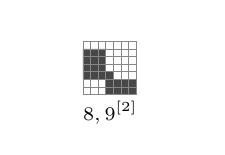
\begin{tikzpicture}[x=1mm,y=1mm,baseline=0mm]
\path[use as bounding box] (0,-.7) rectangle (21.5,11.9);
\begin{scope}[shift={(7.0,3.4)},x=0.97mm,y=0.97mm]
\fill[black!72] (0,5) rectangle (1,6) (1,5) rectangle (2,6) (2,5) rectangle (3,6) (0,4) rectangle (1,5) (1,4) rectangle (2,5) (2,4) rectangle (3,5) (0,3) rectangle (1,4) (1,3) rectangle (2,4) (2,3) rectangle (3,4) (0,2) rectangle (1,3) (1,2) rectangle (2,3) (2,2) rectangle (3,3) (3,2) rectangle (4,3) (3,1) rectangle (4,2) (4,1) rectangle (5,2) (5,1) rectangle (6,2) (6,1) rectangle (7,2) (3,0) rectangle (4,1) (4,0) rectangle (5,1) (5,0) rectangle (6,1) (6,0) rectangle (7,1);
\draw[black!47,line width=.16pt] (0,0)--(0,7) (0,0)--(7,0) (1,0)--(1,7) (0,1)--(7,1) (2,0)--(2,7) (0,2)--(7,2) (3,0)--(3,7) (0,3)--(7,3) (4,0)--(4,7) (0,4)--(7,4) (5,0)--(5,7) (0,5)--(7,5) (6,0)--(6,7) (0,6)--(7,6) (7,0)--(7,7) (0,7)--(7,7);
\end{scope}
\node[inner sep=0pt,font=\scriptsize] at (10.5,1.1) {$8,9^{[2]}$};
\end{tikzpicture} &
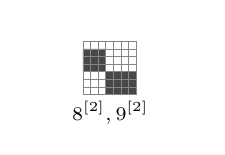
\begin{tikzpicture}[x=1mm,y=1mm,baseline=0mm]
\path[use as bounding box] (0,-.7) rectangle (21.5,11.9);
\begin{scope}[shift={(7.0,3.4)},x=0.97mm,y=0.97mm]
\fill[black!72] (0,5) rectangle (1,6) (1,5) rectangle (2,6) (2,5) rectangle (3,6) (0,4) rectangle (1,5) (1,4) rectangle (2,5) (2,4) rectangle (3,5) (0,3) rectangle (1,4) (1,3) rectangle (2,4) (2,3) rectangle (3,4) (3,2) rectangle (4,3) (4,2) rectangle (5,3) (5,2) rectangle (6,3) (6,2) rectangle (7,3) (3,1) rectangle (4,2) (4,1) rectangle (5,2) (5,1) rectangle (6,2) (6,1) rectangle (7,2) (3,0) rectangle (4,1) (4,0) rectangle (5,1) (5,0) rectangle (6,1) (6,0) rectangle (7,1);
\draw[black!47,line width=.16pt] (0,0)--(0,7) (0,0)--(7,0) (1,0)--(1,7) (0,1)--(7,1) (2,0)--(2,7) (0,2)--(7,2) (3,0)--(3,7) (0,3)--(7,3) (4,0)--(4,7) (0,4)--(7,4) (5,0)--(5,7) (0,5)--(7,5) (6,0)--(6,7) (0,6)--(7,6) (7,0)--(7,7) (0,7)--(7,7);
\end{scope}
\node[inner sep=0pt,font=\scriptsize] at (10.5,1.1) {$8^{[2]},9^{[2]}$};
\end{tikzpicture} \\[.4mm]
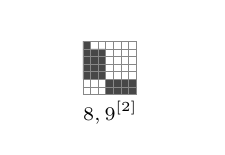
\begin{tikzpicture}[x=1mm,y=1mm,baseline=0mm]
\path[use as bounding box] (0,-.7) rectangle (21.5,11.9);
\begin{scope}[shift={(7.0,3.4)},x=0.97mm,y=0.97mm]
\fill[black!72] (0,6) rectangle (1,7) (0,5) rectangle (1,6) (1,5) rectangle (2,6) (2,5) rectangle (3,6) (0,4) rectangle (1,5) (1,4) rectangle (2,5) (2,4) rectangle (3,5) (0,3) rectangle (1,4) (1,3) rectangle (2,4) (2,3) rectangle (3,4) (0,2) rectangle (1,3) (1,2) rectangle (2,3) (2,2) rectangle (3,3) (3,1) rectangle (4,2) (4,1) rectangle (5,2) (5,1) rectangle (6,2) (6,1) rectangle (7,2) (3,0) rectangle (4,1) (4,0) rectangle (5,1) (5,0) rectangle (6,1) (6,0) rectangle (7,1);
\draw[black!47,line width=.16pt] (0,0)--(0,7) (0,0)--(7,0) (1,0)--(1,7) (0,1)--(7,1) (2,0)--(2,7) (0,2)--(7,2) (3,0)--(3,7) (0,3)--(7,3) (4,0)--(4,7) (0,4)--(7,4) (5,0)--(5,7) (0,5)--(7,5) (6,0)--(6,7) (0,6)--(7,6) (7,0)--(7,7) (0,7)--(7,7);
\end{scope}
\node[inner sep=0pt,font=\scriptsize] at (10.5,1.1) {$8,9^{[2]}$};
\end{tikzpicture} &
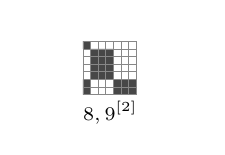
\begin{tikzpicture}[x=1mm,y=1mm,baseline=0mm]
\path[use as bounding box] (0,-.7) rectangle (21.5,11.9);
\begin{scope}[shift={(7.0,3.4)},x=0.97mm,y=0.97mm]
\fill[black!72] (0,6) rectangle (1,7) (1,5) rectangle (2,6) (2,5) rectangle (3,6) (3,5) rectangle (4,6) (1,4) rectangle (2,5) (2,4) rectangle (3,5) (3,4) rectangle (4,5) (1,3) rectangle (2,4) (2,3) rectangle (3,4) (3,3) rectangle (4,4) (1,2) rectangle (2,3) (2,2) rectangle (3,3) (3,2) rectangle (4,3) (0,1) rectangle (1,2) (4,1) rectangle (5,2) (5,1) rectangle (6,2) (6,1) rectangle (7,2) (0,0) rectangle (1,1) (4,0) rectangle (5,1) (5,0) rectangle (6,1) (6,0) rectangle (7,1);
\draw[black!47,line width=.16pt] (0,0)--(0,7) (0,0)--(7,0) (1,0)--(1,7) (0,1)--(7,1) (2,0)--(2,7) (0,2)--(7,2) (3,0)--(3,7) (0,3)--(7,3) (4,0)--(4,7) (0,4)--(7,4) (5,0)--(5,7) (0,5)--(7,5) (6,0)--(6,7) (0,6)--(7,6) (7,0)--(7,7) (0,7)--(7,7);
\end{scope}
\node[inner sep=0pt,font=\scriptsize] at (10.5,1.1) {$8,9^{[2]}$};
\end{tikzpicture} &
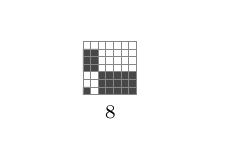
\begin{tikzpicture}[x=1mm,y=1mm,baseline=0mm]
\path[use as bounding box] (0,-.7) rectangle (21.5,11.9);
\begin{scope}[shift={(7.0,3.4)},x=0.97mm,y=0.97mm]
\fill[black!72] (0,5) rectangle (1,6) (1,5) rectangle (2,6) (0,4) rectangle (1,5) (1,4) rectangle (2,5) (0,3) rectangle (1,4) (1,3) rectangle (2,4) (2,2) rectangle (3,3) (3,2) rectangle (4,3) (4,2) rectangle (5,3) (5,2) rectangle (6,3) (6,2) rectangle (7,3) (2,1) rectangle (3,2) (3,1) rectangle (4,2) (4,1) rectangle (5,2) (5,1) rectangle (6,2) (6,1) rectangle (7,2) (0,0) rectangle (1,1) (2,0) rectangle (3,1) (3,0) rectangle (4,1) (4,0) rectangle (5,1) (5,0) rectangle (6,1) (6,0) rectangle (7,1);
\draw[black!47,line width=.16pt] (0,0)--(0,7) (0,0)--(7,0) (1,0)--(1,7) (0,1)--(7,1) (2,0)--(2,7) (0,2)--(7,2) (3,0)--(3,7) (0,3)--(7,3) (4,0)--(4,7) (0,4)--(7,4) (5,0)--(5,7) (0,5)--(7,5) (6,0)--(6,7) (0,6)--(7,6) (7,0)--(7,7) (0,7)--(7,7);
\end{scope}
\node[inner sep=0pt,font=\scriptsize] at (10.5,1.1) {$8$};
\end{tikzpicture} &
\begin{tikzpicture}[x=1mm,y=1mm,baseline=0mm]
\path[use as bounding box] (0,-.7) rectangle (21.5,11.9);
\begin{scope}[shift={(7.0,3.4)},x=0.97mm,y=0.97mm]
\fill[black!72] (0,5) rectangle (1,6) (1,5) rectangle (2,6) (0,4) rectangle (1,5) (1,4) rectangle (2,5) (0,3) rectangle (1,4) (1,3) rectangle (2,4) (2,3) rectangle (3,4) (2,2) rectangle (3,3) (3,2) rectangle (4,3) (4,2) rectangle (5,3) (5,2) rectangle (6,3) (6,2) rectangle (7,3) (2,1) rectangle (3,2) (3,1) rectangle (4,2) (4,1) rectangle (5,2) (5,1) rectangle (6,2) (6,1) rectangle (7,2) (2,0) rectangle (3,1) (3,0) rectangle (4,1) (4,0) rectangle (5,1) (5,0) rectangle (6,1) (6,0) rectangle (7,1);
\draw[black!47,line width=.16pt] (0,0)--(0,7) (0,0)--(7,0) (1,0)--(1,7) (0,1)--(7,1) (2,0)--(2,7) (0,2)--(7,2) (3,0)--(3,7) (0,3)--(7,3) (4,0)--(4,7) (0,4)--(7,4) (5,0)--(5,7) (0,5)--(7,5) (6,0)--(6,7) (0,6)--(7,6) (7,0)--(7,7) (0,7)--(7,7);
\end{scope}
\node[inner sep=0pt,font=\scriptsize] at (10.5,1.1) {$8$};
\end{tikzpicture} &
\begin{tikzpicture}[x=1mm,y=1mm,baseline=0mm]
\path[use as bounding box] (0,-.7) rectangle (21.5,11.9);
\begin{scope}[shift={(7.0,3.4)},x=0.97mm,y=0.97mm]
\fill[black!72] (0,5) rectangle (1,6) (1,5) rectangle (2,6) (2,5) rectangle (3,6) (0,4) rectangle (1,5) (1,4) rectangle (2,5) (2,4) rectangle (3,5) (0,3) rectangle (1,4) (1,3) rectangle (2,4) (2,3) rectangle (3,4) (0,2) rectangle (1,3) (1,2) rectangle (2,3) (2,2) rectangle (3,3) (3,1) rectangle (4,2) (4,1) rectangle (5,2) (5,1) rectangle (6,2) (6,1) rectangle (7,2) (0,0) rectangle (1,1) (1,0) rectangle (2,1) (3,0) rectangle (4,1) (4,0) rectangle (5,1) (5,0) rectangle (6,1) (6,0) rectangle (7,1);
\draw[black!47,line width=.16pt] (0,0)--(0,7) (0,0)--(7,0) (1,0)--(1,7) (0,1)--(7,1) (2,0)--(2,7) (0,2)--(7,2) (3,0)--(3,7) (0,3)--(7,3) (4,0)--(4,7) (0,4)--(7,4) (5,0)--(5,7) (0,5)--(7,5) (6,0)--(6,7) (0,6)--(7,6) (7,0)--(7,7) (0,7)--(7,7);
\end{scope}
\node[inner sep=0pt,font=\scriptsize] at (10.5,1.1) {$8$};
\end{tikzpicture} \\[.4mm]
\begin{tikzpicture}[x=1mm,y=1mm,baseline=0mm]
\path[use as bounding box] (0,-.7) rectangle (21.5,11.9);
\begin{scope}[shift={(7.0,3.4)},x=0.97mm,y=0.97mm]
\fill[black!72] (0,5) rectangle (1,6) (1,5) rectangle (2,6) (2,5) rectangle (3,6) (0,4) rectangle (1,5) (1,4) rectangle (2,5) (2,4) rectangle (3,5) (0,3) rectangle (1,4) (1,3) rectangle (2,4) (2,3) rectangle (3,4) (0,2) rectangle (1,3) (1,2) rectangle (2,3) (2,2) rectangle (3,3) (0,1) rectangle (1,2) (3,1) rectangle (4,2) (4,1) rectangle (5,2) (5,1) rectangle (6,2) (6,1) rectangle (7,2) (0,0) rectangle (1,1) (3,0) rectangle (4,1) (4,0) rectangle (5,1) (5,0) rectangle (6,1) (6,0) rectangle (7,1);
\draw[black!47,line width=.16pt] (0,0)--(0,7) (0,0)--(7,0) (1,0)--(1,7) (0,1)--(7,1) (2,0)--(2,7) (0,2)--(7,2) (3,0)--(3,7) (0,3)--(7,3) (4,0)--(4,7) (0,4)--(7,4) (5,0)--(5,7) (0,5)--(7,5) (6,0)--(6,7) (0,6)--(7,6) (7,0)--(7,7) (0,7)--(7,7);
\end{scope}
\node[inner sep=0pt,font=\scriptsize] at (10.5,1.1) {$8$};
\end{tikzpicture} &
\begin{tikzpicture}[x=1mm,y=1mm,baseline=0mm]
\path[use as bounding box] (0,-.7) rectangle (21.5,11.9);
\begin{scope}[shift={(7.0,3.4)},x=0.97mm,y=0.97mm]
\fill[black!72] (0,5) rectangle (1,6) (1,5) rectangle (2,6) (2,5) rectangle (3,6) (0,4) rectangle (1,5) (1,4) rectangle (2,5) (2,4) rectangle (3,5) (0,3) rectangle (1,4) (1,3) rectangle (2,4) (2,3) rectangle (3,4) (0,2) rectangle (1,3) (1,2) rectangle (2,3) (2,2) rectangle (3,3) (0,1) rectangle (1,2) (3,1) rectangle (4,2) (4,1) rectangle (5,2) (5,1) rectangle (6,2) (6,1) rectangle (7,2) (1,0) rectangle (2,1) (3,0) rectangle (4,1) (4,0) rectangle (5,1) (5,0) rectangle (6,1) (6,0) rectangle (7,1);
\draw[black!47,line width=.16pt] (0,0)--(0,7) (0,0)--(7,0) (1,0)--(1,7) (0,1)--(7,1) (2,0)--(2,7) (0,2)--(7,2) (3,0)--(3,7) (0,3)--(7,3) (4,0)--(4,7) (0,4)--(7,4) (5,0)--(5,7) (0,5)--(7,5) (6,0)--(6,7) (0,6)--(7,6) (7,0)--(7,7) (0,7)--(7,7);
\end{scope}
\node[inner sep=0pt,font=\scriptsize] at (10.5,1.1) {$8$};
\end{tikzpicture} &
\begin{tikzpicture}[x=1mm,y=1mm,baseline=0mm]
\path[use as bounding box] (0,-.7) rectangle (21.5,11.9);
\begin{scope}[shift={(7.0,3.4)},x=0.97mm,y=0.97mm]
\fill[black!72] (0,5) rectangle (1,6) (1,5) rectangle (2,6) (2,5) rectangle (3,6) (0,4) rectangle (1,5) (1,4) rectangle (2,5) (2,4) rectangle (3,5) (0,3) rectangle (1,4) (1,3) rectangle (2,4) (2,3) rectangle (3,4) (0,2) rectangle (1,3) (1,2) rectangle (2,3) (2,2) rectangle (3,3) (3,2) rectangle (4,3) (3,1) rectangle (4,2) (4,1) rectangle (5,2) (5,1) rectangle (6,2) (6,1) rectangle (7,2) (0,0) rectangle (1,1) (3,0) rectangle (4,1) (4,0) rectangle (5,1) (5,0) rectangle (6,1) (6,0) rectangle (7,1);
\draw[black!47,line width=.16pt] (0,0)--(0,7) (0,0)--(7,0) (1,0)--(1,7) (0,1)--(7,1) (2,0)--(2,7) (0,2)--(7,2) (3,0)--(3,7) (0,3)--(7,3) (4,0)--(4,7) (0,4)--(7,4) (5,0)--(5,7) (0,5)--(7,5) (6,0)--(6,7) (0,6)--(7,6) (7,0)--(7,7) (0,7)--(7,7);
\end{scope}
\node[inner sep=0pt,font=\scriptsize] at (10.5,1.1) {$8$};
\end{tikzpicture} &
\begin{tikzpicture}[x=1mm,y=1mm,baseline=0mm]
\path[use as bounding box] (0,-.7) rectangle (21.5,11.9);
\begin{scope}[shift={(7.0,3.4)},x=0.97mm,y=0.97mm]
\fill[black!72] (0,5) rectangle (1,6) (1,5) rectangle (2,6) (2,5) rectangle (3,6) (0,4) rectangle (1,5) (1,4) rectangle (2,5) (2,4) rectangle (3,5) (0,3) rectangle (1,4) (1,3) rectangle (2,4) (2,3) rectangle (3,4) (0,2) rectangle (1,3) (1,2) rectangle (2,3) (2,2) rectangle (3,3) (3,2) rectangle (4,3) (4,2) rectangle (5,3) (3,1) rectangle (4,2) (4,1) rectangle (5,2) (5,1) rectangle (6,2) (6,1) rectangle (7,2) (3,0) rectangle (4,1) (4,0) rectangle (5,1) (5,0) rectangle (6,1) (6,0) rectangle (7,1);
\draw[black!47,line width=.16pt] (0,0)--(0,7) (0,0)--(7,0) (1,0)--(1,7) (0,1)--(7,1) (2,0)--(2,7) (0,2)--(7,2) (3,0)--(3,7) (0,3)--(7,3) (4,0)--(4,7) (0,4)--(7,4) (5,0)--(5,7) (0,5)--(7,5) (6,0)--(6,7) (0,6)--(7,6) (7,0)--(7,7) (0,7)--(7,7);
\end{scope}
\node[inner sep=0pt,font=\scriptsize] at (10.5,1.1) {$8$};
\end{tikzpicture} &
\begin{tikzpicture}[x=1mm,y=1mm,baseline=0mm]
\path[use as bounding box] (0,-.7) rectangle (21.5,11.9);
\begin{scope}[shift={(7.0,3.4)},x=0.97mm,y=0.97mm]
\fill[black!72] (0,5) rectangle (1,6) (1,5) rectangle (2,6) (2,5) rectangle (3,6) (0,4) rectangle (1,5) (1,4) rectangle (2,5) (2,4) rectangle (3,5) (0,3) rectangle (1,4) (1,3) rectangle (2,4) (2,3) rectangle (3,4) (3,2) rectangle (4,3) (4,2) rectangle (5,3) (5,2) rectangle (6,3) (6,2) rectangle (7,3) (3,1) rectangle (4,2) (4,1) rectangle (5,2) (5,1) rectangle (6,2) (6,1) rectangle (7,2) (0,0) rectangle (1,1) (3,0) rectangle (4,1) (4,0) rectangle (5,1) (5,0) rectangle (6,1) (6,0) rectangle (7,1);
\draw[black!47,line width=.16pt] (0,0)--(0,7) (0,0)--(7,0) (1,0)--(1,7) (0,1)--(7,1) (2,0)--(2,7) (0,2)--(7,2) (3,0)--(3,7) (0,3)--(7,3) (4,0)--(4,7) (0,4)--(7,4) (5,0)--(5,7) (0,5)--(7,5) (6,0)--(6,7) (0,6)--(7,6) (7,0)--(7,7) (0,7)--(7,7);
\end{scope}
\node[inner sep=0pt,font=\scriptsize] at (10.5,1.1) {$8^{[2]}$};
\end{tikzpicture} \\[.4mm]
\begin{tikzpicture}[x=1mm,y=1mm,baseline=0mm]
\path[use as bounding box] (0,-.7) rectangle (21.5,11.9);
\begin{scope}[shift={(7.0,3.4)},x=0.97mm,y=0.97mm]
\fill[black!72] (0,5) rectangle (1,6) (1,5) rectangle (2,6) (2,5) rectangle (3,6) (0,4) rectangle (1,5) (1,4) rectangle (2,5) (2,4) rectangle (3,5) (0,3) rectangle (1,4) (1,3) rectangle (2,4) (2,3) rectangle (3,4) (3,3) rectangle (4,4) (0,2) rectangle (1,3) (1,2) rectangle (2,3) (2,2) rectangle (3,3) (3,2) rectangle (4,3) (3,1) rectangle (4,2) (4,1) rectangle (5,2) (5,1) rectangle (6,2) (6,1) rectangle (7,2) (3,0) rectangle (4,1) (4,0) rectangle (5,1) (5,0) rectangle (6,1) (6,0) rectangle (7,1);
\draw[black!47,line width=.16pt] (0,0)--(0,7) (0,0)--(7,0) (1,0)--(1,7) (0,1)--(7,1) (2,0)--(2,7) (0,2)--(7,2) (3,0)--(3,7) (0,3)--(7,3) (4,0)--(4,7) (0,4)--(7,4) (5,0)--(5,7) (0,5)--(7,5) (6,0)--(6,7) (0,6)--(7,6) (7,0)--(7,7) (0,7)--(7,7);
\end{scope}
\node[inner sep=0pt,font=\scriptsize] at (10.5,1.1) {$8$};
\end{tikzpicture} &
\begin{tikzpicture}[x=1mm,y=1mm,baseline=0mm]
\path[use as bounding box] (0,-.7) rectangle (21.5,11.9);
\begin{scope}[shift={(7.0,3.4)},x=0.97mm,y=0.97mm]
\fill[black!72] (0,5) rectangle (1,6) (1,5) rectangle (2,6) (2,5) rectangle (3,6) (0,4) rectangle (1,5) (1,4) rectangle (2,5) (2,4) rectangle (3,5) (0,3) rectangle (1,4) (1,3) rectangle (2,4) (2,3) rectangle (3,4) (3,3) rectangle (4,4) (0,2) rectangle (1,3) (1,2) rectangle (2,3) (2,2) rectangle (3,3) (4,2) rectangle (5,3) (3,1) rectangle (4,2) (4,1) rectangle (5,2) (5,1) rectangle (6,2) (6,1) rectangle (7,2) (3,0) rectangle (4,1) (4,0) rectangle (5,1) (5,0) rectangle (6,1) (6,0) rectangle (7,1);
\draw[black!47,line width=.16pt] (0,0)--(0,7) (0,0)--(7,0) (1,0)--(1,7) (0,1)--(7,1) (2,0)--(2,7) (0,2)--(7,2) (3,0)--(3,7) (0,3)--(7,3) (4,0)--(4,7) (0,4)--(7,4) (5,0)--(5,7) (0,5)--(7,5) (6,0)--(6,7) (0,6)--(7,6) (7,0)--(7,7) (0,7)--(7,7);
\end{scope}
\node[inner sep=0pt,font=\scriptsize] at (10.5,1.1) {$8$};
\end{tikzpicture} &
\begin{tikzpicture}[x=1mm,y=1mm,baseline=0mm]
\path[use as bounding box] (0,-.7) rectangle (21.5,11.9);
\begin{scope}[shift={(7.0,3.4)},x=0.97mm,y=0.97mm]
\fill[black!72] (0,5) rectangle (1,6) (1,5) rectangle (2,6) (2,5) rectangle (3,6) (0,4) rectangle (1,5) (1,4) rectangle (2,5) (2,4) rectangle (3,5) (0,3) rectangle (1,4) (1,3) rectangle (2,4) (2,3) rectangle (3,4) (3,3) rectangle (4,4) (3,2) rectangle (4,3) (4,2) rectangle (5,3) (5,2) rectangle (6,3) (6,2) rectangle (7,3) (3,1) rectangle (4,2) (4,1) rectangle (5,2) (5,1) rectangle (6,2) (6,1) rectangle (7,2) (3,0) rectangle (4,1) (4,0) rectangle (5,1) (5,0) rectangle (6,1) (6,0) rectangle (7,1);
\draw[black!47,line width=.16pt] (0,0)--(0,7) (0,0)--(7,0) (1,0)--(1,7) (0,1)--(7,1) (2,0)--(2,7) (0,2)--(7,2) (3,0)--(3,7) (0,3)--(7,3) (4,0)--(4,7) (0,4)--(7,4) (5,0)--(5,7) (0,5)--(7,5) (6,0)--(6,7) (0,6)--(7,6) (7,0)--(7,7) (0,7)--(7,7);
\end{scope}
\node[inner sep=0pt,font=\scriptsize] at (10.5,1.1) {$8^{[2]}$};
\end{tikzpicture} &
\begin{tikzpicture}[x=1mm,y=1mm,baseline=0mm]
\path[use as bounding box] (0,-.7) rectangle (21.5,11.9);
\begin{scope}[shift={(7.0,3.4)},x=0.97mm,y=0.97mm]
\fill[black!72] (0,5) rectangle (1,6) (1,5) rectangle (2,6) (2,5) rectangle (3,6) (0,4) rectangle (1,5) (1,4) rectangle (2,5) (2,4) rectangle (3,5) (3,3) rectangle (4,4) (4,3) rectangle (5,4) (5,3) rectangle (6,4) (6,3) rectangle (7,4) (3,2) rectangle (4,3) (4,2) rectangle (5,3) (5,2) rectangle (6,3) (6,2) rectangle (7,3) (3,1) rectangle (4,2) (4,1) rectangle (5,2) (5,1) rectangle (6,2) (6,1) rectangle (7,2) (3,0) rectangle (4,1) (4,0) rectangle (5,1) (5,0) rectangle (6,1) (6,0) rectangle (7,1);
\draw[black!47,line width=.16pt] (0,0)--(0,7) (0,0)--(7,0) (1,0)--(1,7) (0,1)--(7,1) (2,0)--(2,7) (0,2)--(7,2) (3,0)--(3,7) (0,3)--(7,3) (4,0)--(4,7) (0,4)--(7,4) (5,0)--(5,7) (0,5)--(7,5) (6,0)--(6,7) (0,6)--(7,6) (7,0)--(7,7) (0,7)--(7,7);
\end{scope}
\node[inner sep=0pt,font=\scriptsize] at (10.5,1.1) {$8^{[2]}$};
\end{tikzpicture} &
\begin{tikzpicture}[x=1mm,y=1mm,baseline=0mm]
\path[use as bounding box] (0,-.7) rectangle (21.5,11.9);
\begin{scope}[shift={(7.0,3.4)},x=0.97mm,y=0.97mm]
\fill[black!72] (0,6) rectangle (1,7) (0,5) rectangle (1,6) (1,5) rectangle (2,6) (0,4) rectangle (1,5) (1,4) rectangle (2,5) (0,3) rectangle (1,4) (1,3) rectangle (2,4) (2,2) rectangle (3,3) (3,2) rectangle (4,3) (4,2) rectangle (5,3) (5,2) rectangle (6,3) (6,2) rectangle (7,3) (2,1) rectangle (3,2) (3,1) rectangle (4,2) (4,1) rectangle (5,2) (5,1) rectangle (6,2) (6,1) rectangle (7,2) (2,0) rectangle (3,1) (3,0) rectangle (4,1) (4,0) rectangle (5,1) (5,0) rectangle (6,1) (6,0) rectangle (7,1);
\draw[black!47,line width=.16pt] (0,0)--(0,7) (0,0)--(7,0) (1,0)--(1,7) (0,1)--(7,1) (2,0)--(2,7) (0,2)--(7,2) (3,0)--(3,7) (0,3)--(7,3) (4,0)--(4,7) (0,4)--(7,4) (5,0)--(5,7) (0,5)--(7,5) (6,0)--(6,7) (0,6)--(7,6) (7,0)--(7,7) (0,7)--(7,7);
\end{scope}
\node[inner sep=0pt,font=\scriptsize] at (10.5,1.1) {$8$};
\end{tikzpicture} \\[.4mm]
\begin{tikzpicture}[x=1mm,y=1mm,baseline=0mm]
\path[use as bounding box] (0,-.7) rectangle (21.5,11.9);
\begin{scope}[shift={(7.0,3.4)},x=0.97mm,y=0.97mm]
\fill[black!72] (0,6) rectangle (1,7) (1,5) rectangle (2,6) (2,5) rectangle (3,6) (1,4) rectangle (2,5) (2,4) rectangle (3,5) (1,3) rectangle (2,4) (2,3) rectangle (3,4) (0,2) rectangle (1,3) (3,2) rectangle (4,3) (4,2) rectangle (5,3) (5,2) rectangle (6,3) (6,2) rectangle (7,3) (0,1) rectangle (1,2) (3,1) rectangle (4,2) (4,1) rectangle (5,2) (5,1) rectangle (6,2) (6,1) rectangle (7,2) (0,0) rectangle (1,1) (3,0) rectangle (4,1) (4,0) rectangle (5,1) (5,0) rectangle (6,1) (6,0) rectangle (7,1);
\draw[black!47,line width=.16pt] (0,0)--(0,7) (0,0)--(7,0) (1,0)--(1,7) (0,1)--(7,1) (2,0)--(2,7) (0,2)--(7,2) (3,0)--(3,7) (0,3)--(7,3) (4,0)--(4,7) (0,4)--(7,4) (5,0)--(5,7) (0,5)--(7,5) (6,0)--(6,7) (0,6)--(7,6) (7,0)--(7,7) (0,7)--(7,7);
\end{scope}
\node[inner sep=0pt,font=\scriptsize] at (10.5,1.1) {$8$};
\end{tikzpicture} &
\begin{tikzpicture}[x=1mm,y=1mm,baseline=0mm]
\path[use as bounding box] (0,-.7) rectangle (21.5,11.9);
\begin{scope}[shift={(7.0,3.4)},x=0.97mm,y=0.97mm]
\fill[black!72] (0,6) rectangle (1,7) (0,5) rectangle (1,6) (1,5) rectangle (2,6) (2,5) rectangle (3,6) (0,4) rectangle (1,5) (1,4) rectangle (2,5) (2,4) rectangle (3,5) (0,3) rectangle (1,4) (1,3) rectangle (2,4) (2,3) rectangle (3,4) (0,2) rectangle (1,3) (1,2) rectangle (2,3) (2,2) rectangle (3,3) (3,1) rectangle (4,2) (4,1) rectangle (5,2) (5,1) rectangle (6,2) (6,1) rectangle (7,2) (0,0) rectangle (1,1) (3,0) rectangle (4,1) (4,0) rectangle (5,1) (5,0) rectangle (6,1) (6,0) rectangle (7,1);
\draw[black!47,line width=.16pt] (0,0)--(0,7) (0,0)--(7,0) (1,0)--(1,7) (0,1)--(7,1) (2,0)--(2,7) (0,2)--(7,2) (3,0)--(3,7) (0,3)--(7,3) (4,0)--(4,7) (0,4)--(7,4) (5,0)--(5,7) (0,5)--(7,5) (6,0)--(6,7) (0,6)--(7,6) (7,0)--(7,7) (0,7)--(7,7);
\end{scope}
\node[inner sep=0pt,font=\scriptsize] at (10.5,1.1) {$8$};
\end{tikzpicture} &
\begin{tikzpicture}[x=1mm,y=1mm,baseline=0mm]
\path[use as bounding box] (0,-.7) rectangle (21.5,11.9);
\begin{scope}[shift={(7.0,3.4)},x=0.97mm,y=0.97mm]
\fill[black!72] (0,6) rectangle (1,7) (0,5) rectangle (1,6) (1,5) rectangle (2,6) (2,5) rectangle (3,6) (0,4) rectangle (1,5) (1,4) rectangle (2,5) (2,4) rectangle (3,5) (0,3) rectangle (1,4) (1,3) rectangle (2,4) (2,3) rectangle (3,4) (0,2) rectangle (1,3) (1,2) rectangle (2,3) (2,2) rectangle (3,3) (3,1) rectangle (4,2) (4,1) rectangle (5,2) (5,1) rectangle (6,2) (6,1) rectangle (7,2) (1,0) rectangle (2,1) (3,0) rectangle (4,1) (4,0) rectangle (5,1) (5,0) rectangle (6,1) (6,0) rectangle (7,1);
\draw[black!47,line width=.16pt] (0,0)--(0,7) (0,0)--(7,0) (1,0)--(1,7) (0,1)--(7,1) (2,0)--(2,7) (0,2)--(7,2) (3,0)--(3,7) (0,3)--(7,3) (4,0)--(4,7) (0,4)--(7,4) (5,0)--(5,7) (0,5)--(7,5) (6,0)--(6,7) (0,6)--(7,6) (7,0)--(7,7) (0,7)--(7,7);
\end{scope}
\node[inner sep=0pt,font=\scriptsize] at (10.5,1.1) {$8^{[2]}$};
\end{tikzpicture} &
\begin{tikzpicture}[x=1mm,y=1mm,baseline=0mm]
\path[use as bounding box] (0,-.7) rectangle (21.5,11.9);
\begin{scope}[shift={(7.0,3.4)},x=0.97mm,y=0.97mm]
\fill[black!72] (0,6) rectangle (1,7) (0,5) rectangle (1,6) (1,5) rectangle (2,6) (2,5) rectangle (3,6) (0,4) rectangle (1,5) (1,4) rectangle (2,5) (2,4) rectangle (3,5) (0,3) rectangle (1,4) (1,3) rectangle (2,4) (2,3) rectangle (3,4) (0,2) rectangle (1,3) (1,2) rectangle (2,3) (2,2) rectangle (3,3) (3,2) rectangle (4,3) (3,1) rectangle (4,2) (4,1) rectangle (5,2) (5,1) rectangle (6,2) (6,1) rectangle (7,2) (3,0) rectangle (4,1) (4,0) rectangle (5,1) (5,0) rectangle (6,1) (6,0) rectangle (7,1);
\draw[black!47,line width=.16pt] (0,0)--(0,7) (0,0)--(7,0) (1,0)--(1,7) (0,1)--(7,1) (2,0)--(2,7) (0,2)--(7,2) (3,0)--(3,7) (0,3)--(7,3) (4,0)--(4,7) (0,4)--(7,4) (5,0)--(5,7) (0,5)--(7,5) (6,0)--(6,7) (0,6)--(7,6) (7,0)--(7,7) (0,7)--(7,7);
\end{scope}
\node[inner sep=0pt,font=\scriptsize] at (10.5,1.1) {$8$};
\end{tikzpicture} &
\begin{tikzpicture}[x=1mm,y=1mm,baseline=0mm]
\path[use as bounding box] (0,-.7) rectangle (21.5,11.9);
\begin{scope}[shift={(7.0,3.4)},x=0.97mm,y=0.97mm]
\fill[black!72] (0,6) rectangle (1,7) (0,5) rectangle (1,6) (1,5) rectangle (2,6) (2,5) rectangle (3,6) (0,4) rectangle (1,5) (1,4) rectangle (2,5) (2,4) rectangle (3,5) (0,3) rectangle (1,4) (1,3) rectangle (2,4) (2,3) rectangle (3,4) (3,2) rectangle (4,3) (4,2) rectangle (5,3) (5,2) rectangle (6,3) (6,2) rectangle (7,3) (3,1) rectangle (4,2) (4,1) rectangle (5,2) (5,1) rectangle (6,2) (6,1) rectangle (7,2) (3,0) rectangle (4,1) (4,0) rectangle (5,1) (5,0) rectangle (6,1) (6,0) rectangle (7,1);
\draw[black!47,line width=.16pt] (0,0)--(0,7) (0,0)--(7,0) (1,0)--(1,7) (0,1)--(7,1) (2,0)--(2,7) (0,2)--(7,2) (3,0)--(3,7) (0,3)--(7,3) (4,0)--(4,7) (0,4)--(7,4) (5,0)--(5,7) (0,5)--(7,5) (6,0)--(6,7) (0,6)--(7,6) (7,0)--(7,7) (0,7)--(7,7);
\end{scope}
\node[inner sep=0pt,font=\scriptsize] at (10.5,1.1) {$8^{[2]}$};
\end{tikzpicture} \\[.4mm]
\begin{tikzpicture}[x=1mm,y=1mm,baseline=0mm]
\path[use as bounding box] (0,-.7) rectangle (21.5,11.9);
\begin{scope}[shift={(7.0,3.4)},x=0.97mm,y=0.97mm]
\fill[black!72] (0,6) rectangle (1,7) (1,5) rectangle (2,6) (2,5) rectangle (3,6) (3,5) rectangle (4,6) (1,4) rectangle (2,5) (2,4) rectangle (3,5) (3,4) rectangle (4,5) (1,3) rectangle (2,4) (2,3) rectangle (3,4) (3,3) rectangle (4,4) (1,2) rectangle (2,3) (2,2) rectangle (3,3) (3,2) rectangle (4,3) (0,1) rectangle (1,2) (4,1) rectangle (5,2) (5,1) rectangle (6,2) (6,1) rectangle (7,2) (0,0) rectangle (1,1) (1,0) rectangle (2,1) (4,0) rectangle (5,1) (5,0) rectangle (6,1) (6,0) rectangle (7,1);
\draw[black!47,line width=.16pt] (0,0)--(0,7) (0,0)--(7,0) (1,0)--(1,7) (0,1)--(7,1) (2,0)--(2,7) (0,2)--(7,2) (3,0)--(3,7) (0,3)--(7,3) (4,0)--(4,7) (0,4)--(7,4) (5,0)--(5,7) (0,5)--(7,5) (6,0)--(6,7) (0,6)--(7,6) (7,0)--(7,7) (0,7)--(7,7);
\end{scope}
\node[inner sep=0pt,font=\scriptsize] at (10.5,1.1) {$8$};
\end{tikzpicture} &
\begin{tikzpicture}[x=1mm,y=1mm,baseline=0mm]
\path[use as bounding box] (0,-.7) rectangle (21.5,11.9);
\begin{scope}[shift={(7.0,3.4)},x=0.97mm,y=0.97mm]
\fill[black!72] (0,6) rectangle (1,7) (1,5) rectangle (2,6) (2,5) rectangle (3,6) (3,5) rectangle (4,6) (1,4) rectangle (2,5) (2,4) rectangle (3,5) (3,4) rectangle (4,5) (1,3) rectangle (2,4) (2,3) rectangle (3,4) (3,3) rectangle (4,4) (0,2) rectangle (1,3) (1,2) rectangle (2,3) (2,2) rectangle (3,3) (3,2) rectangle (4,3) (0,1) rectangle (1,2) (4,1) rectangle (5,2) (5,1) rectangle (6,2) (6,1) rectangle (7,2) (0,0) rectangle (1,1) (4,0) rectangle (5,1) (5,0) rectangle (6,1) (6,0) rectangle (7,1);
\draw[black!47,line width=.16pt] (0,0)--(0,7) (0,0)--(7,0) (1,0)--(1,7) (0,1)--(7,1) (2,0)--(2,7) (0,2)--(7,2) (3,0)--(3,7) (0,3)--(7,3) (4,0)--(4,7) (0,4)--(7,4) (5,0)--(5,7) (0,5)--(7,5) (6,0)--(6,7) (0,6)--(7,6) (7,0)--(7,7) (0,7)--(7,7);
\end{scope}
\node[inner sep=0pt,font=\scriptsize] at (10.5,1.1) {$8$};
\end{tikzpicture} &
\begin{tikzpicture}[x=1mm,y=1mm,baseline=0mm]
\path[use as bounding box] (0,-.7) rectangle (21.5,11.9);
\begin{scope}[shift={(7.0,3.4)},x=0.97mm,y=0.97mm]
\fill[black!72] (0,6) rectangle (1,7) (1,5) rectangle (2,6) (2,5) rectangle (3,6) (3,5) rectangle (4,6) (1,4) rectangle (2,5) (2,4) rectangle (3,5) (3,4) rectangle (4,5) (1,3) rectangle (2,4) (2,3) rectangle (3,4) (3,3) rectangle (4,4) (1,2) rectangle (2,3) (2,2) rectangle (3,3) (3,2) rectangle (4,3) (4,2) rectangle (5,3) (0,1) rectangle (1,2) (4,1) rectangle (5,2) (5,1) rectangle (6,2) (6,1) rectangle (7,2) (0,0) rectangle (1,1) (4,0) rectangle (5,1) (5,0) rectangle (6,1) (6,0) rectangle (7,1);
\draw[black!47,line width=.16pt] (0,0)--(0,7) (0,0)--(7,0) (1,0)--(1,7) (0,1)--(7,1) (2,0)--(2,7) (0,2)--(7,2) (3,0)--(3,7) (0,3)--(7,3) (4,0)--(4,7) (0,4)--(7,4) (5,0)--(5,7) (0,5)--(7,5) (6,0)--(6,7) (0,6)--(7,6) (7,0)--(7,7) (0,7)--(7,7);
\end{scope}
\node[inner sep=0pt,font=\scriptsize] at (10.5,1.1) {$8^{[2]}$};
\end{tikzpicture} &
\begin{tikzpicture}[x=1mm,y=1mm,baseline=0mm]
\path[use as bounding box] (0,-.7) rectangle (21.5,11.9);
\begin{scope}[shift={(7.0,3.4)},x=0.97mm,y=0.97mm]
\fill[black!72] (0,6) rectangle (1,7) (1,5) rectangle (2,6) (2,5) rectangle (3,6) (3,5) rectangle (4,6) (1,4) rectangle (2,5) (2,4) rectangle (3,5) (3,4) rectangle (4,5) (1,3) rectangle (2,4) (2,3) rectangle (3,4) (3,3) rectangle (4,4) (0,2) rectangle (1,3) (4,2) rectangle (5,3) (5,2) rectangle (6,3) (6,2) rectangle (7,3) (0,1) rectangle (1,2) (4,1) rectangle (5,2) (5,1) rectangle (6,2) (6,1) rectangle (7,2) (0,0) rectangle (1,1) (4,0) rectangle (5,1) (5,0) rectangle (6,1) (6,0) rectangle (7,1);
\draw[black!47,line width=.16pt] (0,0)--(0,7) (0,0)--(7,0) (1,0)--(1,7) (0,1)--(7,1) (2,0)--(2,7) (0,2)--(7,2) (3,0)--(3,7) (0,3)--(7,3) (4,0)--(4,7) (0,4)--(7,4) (5,0)--(5,7) (0,5)--(7,5) (6,0)--(6,7) (0,6)--(7,6) (7,0)--(7,7) (0,7)--(7,7);
\end{scope}
\node[inner sep=0pt,font=\scriptsize] at (10.5,1.1) {$8^{[2]}$};
\end{tikzpicture} &
\begin{tikzpicture}[x=1mm,y=1mm,baseline=0mm]
\path[use as bounding box] (0,-.7) rectangle (21.5,11.9);
\begin{scope}[shift={(7.0,3.4)},x=0.97mm,y=0.97mm]
\fill[black!72] (0,6) rectangle (1,7) (1,6) rectangle (2,7) (0,5) rectangle (1,6) (1,5) rectangle (2,6) (0,4) rectangle (1,5) (1,4) rectangle (2,5) (0,3) rectangle (1,4) (1,3) rectangle (2,4) (2,2) rectangle (3,3) (3,2) rectangle (4,3) (4,2) rectangle (5,3) (5,2) rectangle (6,3) (2,1) rectangle (3,2) (3,1) rectangle (4,2) (4,1) rectangle (5,2) (5,1) rectangle (6,2) (6,1) rectangle (7,2) (2,0) rectangle (3,1) (3,0) rectangle (4,1) (4,0) rectangle (5,1) (5,0) rectangle (6,1) (6,0) rectangle (7,1);
\draw[black!47,line width=.16pt] (0,0)--(0,7) (0,0)--(7,0) (1,0)--(1,7) (0,1)--(7,1) (2,0)--(2,7) (0,2)--(7,2) (3,0)--(3,7) (0,3)--(7,3) (4,0)--(4,7) (0,4)--(7,4) (5,0)--(5,7) (0,5)--(7,5) (6,0)--(6,7) (0,6)--(7,6) (7,0)--(7,7) (0,7)--(7,7);
\end{scope}
\node[inner sep=0pt,font=\scriptsize] at (10.5,1.1) {$8$};
\end{tikzpicture} \\[.4mm]
\begin{tikzpicture}[x=1mm,y=1mm,baseline=0mm]
\path[use as bounding box] (0,-.7) rectangle (21.5,11.9);
\begin{scope}[shift={(7.0,3.4)},x=0.97mm,y=0.97mm]
\fill[black!72] (0,6) rectangle (1,7) (1,6) rectangle (2,7) (0,5) rectangle (1,6) (1,5) rectangle (2,6) (0,4) rectangle (1,5) (1,4) rectangle (2,5) (0,3) rectangle (1,4) (1,3) rectangle (2,4) (2,3) rectangle (3,4) (3,2) rectangle (4,3) (4,2) rectangle (5,3) (5,2) rectangle (6,3) (6,2) rectangle (7,3) (3,1) rectangle (4,2) (4,1) rectangle (5,2) (5,1) rectangle (6,2) (6,1) rectangle (7,2) (2,0) rectangle (3,1) (3,0) rectangle (4,1) (4,0) rectangle (5,1) (5,0) rectangle (6,1) (6,0) rectangle (7,1);
\draw[black!47,line width=.16pt] (0,0)--(0,7) (0,0)--(7,0) (1,0)--(1,7) (0,1)--(7,1) (2,0)--(2,7) (0,2)--(7,2) (3,0)--(3,7) (0,3)--(7,3) (4,0)--(4,7) (0,4)--(7,4) (5,0)--(5,7) (0,5)--(7,5) (6,0)--(6,7) (0,6)--(7,6) (7,0)--(7,7) (0,7)--(7,7);
\end{scope}
\node[inner sep=0pt,font=\scriptsize] at (10.5,1.1) {$8$};
\end{tikzpicture} &
\begin{tikzpicture}[x=1mm,y=1mm,baseline=0mm]
\path[use as bounding box] (0,-.7) rectangle (21.5,11.9);
\begin{scope}[shift={(7.0,3.4)},x=0.97mm,y=0.97mm]
\fill[black!72] (0,6) rectangle (1,7) (1,6) rectangle (2,7) (0,5) rectangle (1,6) (1,5) rectangle (2,6) (0,4) rectangle (1,5) (1,4) rectangle (2,5) (2,4) rectangle (3,5) (0,3) rectangle (1,4) (1,3) rectangle (2,4) (2,3) rectangle (3,4) (3,2) rectangle (4,3) (4,2) rectangle (5,3) (5,2) rectangle (6,3) (6,2) rectangle (7,3) (3,1) rectangle (4,2) (4,1) rectangle (5,2) (5,1) rectangle (6,2) (6,1) rectangle (7,2) (3,0) rectangle (4,1) (4,0) rectangle (5,1) (5,0) rectangle (6,1) (6,0) rectangle (7,1);
\draw[black!47,line width=.16pt] (0,0)--(0,7) (0,0)--(7,0) (1,0)--(1,7) (0,1)--(7,1) (2,0)--(2,7) (0,2)--(7,2) (3,0)--(3,7) (0,3)--(7,3) (4,0)--(4,7) (0,4)--(7,4) (5,0)--(5,7) (0,5)--(7,5) (6,0)--(6,7) (0,6)--(7,6) (7,0)--(7,7) (0,7)--(7,7);
\end{scope}
\node[inner sep=0pt,font=\scriptsize] at (10.5,1.1) {$8$};
\end{tikzpicture} \\[.4mm]
\end{tabular}
\caption{Cross adjacencies tested in the connected case, part 2 of 2.}
\label{fig:nine-qfourteen-connected-last}
\end{figure}

\begin{figure}[!htbp]
\centering
\begin{tabular}{@{}c@{\hspace{1.6mm}}c@{\hspace{1.6mm}}c@{\hspace{1.6mm}}c@{\hspace{1.6mm}}c@{}}
\begin{tikzpicture}[x=1mm,y=1mm,baseline=0mm]
\path[use as bounding box] (0,-.7) rectangle (21.5,11.9);
\begin{scope}[shift={(7.0,3.4)},x=0.97mm,y=0.97mm]
\fill[black!72] (1,6) rectangle (2,7) (2,6) rectangle (3,7) (3,6) rectangle (4,7) (4,6) rectangle (5,7) (5,6) rectangle (6,7) (6,6) rectangle (7,7) (1,5) rectangle (2,6) (2,5) rectangle (3,6) (3,5) rectangle (4,6) (4,5) rectangle (5,6) (5,5) rectangle (6,6) (6,5) rectangle (7,6) (1,4) rectangle (2,5) (2,4) rectangle (3,5) (3,4) rectangle (4,5) (4,4) rectangle (5,5) (5,4) rectangle (6,5) (6,4) rectangle (7,5) (1,3) rectangle (2,4) (2,3) rectangle (3,4) (3,3) rectangle (4,4) (4,3) rectangle (5,4) (5,3) rectangle (6,4) (6,3) rectangle (7,4) (0,2) rectangle (1,3) (0,1) rectangle (1,2) (0,0) rectangle (1,1);
\draw[black!47,line width=.16pt] (0,0)--(0,7) (0,0)--(7,0) (1,0)--(1,7) (0,1)--(7,1) (2,0)--(2,7) (0,2)--(7,2) (3,0)--(3,7) (0,3)--(7,3) (4,0)--(4,7) (0,4)--(7,4) (5,0)--(5,7) (0,5)--(7,5) (6,0)--(6,7) (0,6)--(7,6) (7,0)--(7,7) (0,7)--(7,7);
\end{scope}
\node[inner sep=0pt,font=\scriptsize] at (10.5,1.1) {$0\!-\!3^{[2]}$};
\end{tikzpicture} &
\begin{tikzpicture}[x=1mm,y=1mm,baseline=0mm]
\path[use as bounding box] (0,-.7) rectangle (21.5,11.9);
\begin{scope}[shift={(7.0,3.4)},x=0.97mm,y=0.97mm]
\fill[black!72] (2,6) rectangle (3,7) (3,6) rectangle (4,7) (4,6) rectangle (5,7) (5,6) rectangle (6,7) (6,6) rectangle (7,7) (2,5) rectangle (3,6) (3,5) rectangle (4,6) (4,5) rectangle (5,6) (5,5) rectangle (6,6) (6,5) rectangle (7,6) (2,4) rectangle (3,5) (3,4) rectangle (4,5) (4,4) rectangle (5,5) (5,4) rectangle (6,5) (6,4) rectangle (7,5) (2,3) rectangle (3,4) (3,3) rectangle (4,4) (4,3) rectangle (5,4) (5,3) rectangle (6,4) (6,3) rectangle (7,4) (0,2) rectangle (1,3) (1,2) rectangle (2,3) (0,1) rectangle (1,2) (1,1) rectangle (2,2) (0,0) rectangle (1,1) (1,0) rectangle (2,1);
\draw[black!47,line width=.16pt] (0,0)--(0,7) (0,0)--(7,0) (1,0)--(1,7) (0,1)--(7,1) (2,0)--(2,7) (0,2)--(7,2) (3,0)--(3,7) (0,3)--(7,3) (4,0)--(4,7) (0,4)--(7,4) (5,0)--(5,7) (0,5)--(7,5) (6,0)--(6,7) (0,6)--(7,6) (7,0)--(7,7) (0,7)--(7,7);
\end{scope}
\node[inner sep=0pt,font=\scriptsize] at (10.5,1.1) {$0\!-\!4^{[2]}$};
\end{tikzpicture} &
\begin{tikzpicture}[x=1mm,y=1mm,baseline=0mm]
\path[use as bounding box] (0,-.7) rectangle (21.5,11.9);
\begin{scope}[shift={(7.0,3.4)},x=0.97mm,y=0.97mm]
\fill[black!72] (3,6) rectangle (4,7) (4,6) rectangle (5,7) (5,6) rectangle (6,7) (6,6) rectangle (7,7) (3,5) rectangle (4,6) (4,5) rectangle (5,6) (5,5) rectangle (6,6) (6,5) rectangle (7,6) (3,4) rectangle (4,5) (4,4) rectangle (5,5) (5,4) rectangle (6,5) (6,4) rectangle (7,5) (3,3) rectangle (4,4) (4,3) rectangle (5,4) (5,3) rectangle (6,4) (6,3) rectangle (7,4) (0,2) rectangle (1,3) (1,2) rectangle (2,3) (2,2) rectangle (3,3) (0,1) rectangle (1,2) (1,1) rectangle (2,2) (2,1) rectangle (3,2) (0,0) rectangle (1,1) (1,0) rectangle (2,1) (2,0) rectangle (3,1);
\draw[black!47,line width=.16pt] (0,0)--(0,7) (0,0)--(7,0) (1,0)--(1,7) (0,1)--(7,1) (2,0)--(2,7) (0,2)--(7,2) (3,0)--(3,7) (0,3)--(7,3) (4,0)--(4,7) (0,4)--(7,4) (5,0)--(5,7) (0,5)--(7,5) (6,0)--(6,7) (0,6)--(7,6) (7,0)--(7,7) (0,7)--(7,7);
\end{scope}
\node[inner sep=0pt,font=\scriptsize] at (10.5,1.1) {$0\!-\!5$};
\end{tikzpicture} &
\begin{tikzpicture}[x=1mm,y=1mm,baseline=0mm]
\path[use as bounding box] (0,-.7) rectangle (21.5,11.9);
\begin{scope}[shift={(7.0,3.4)},x=0.97mm,y=0.97mm]
\fill[black!72] (4,6) rectangle (5,7) (5,6) rectangle (6,7) (6,6) rectangle (7,7) (4,5) rectangle (5,6) (5,5) rectangle (6,6) (6,5) rectangle (7,6) (4,4) rectangle (5,5) (5,4) rectangle (6,5) (6,4) rectangle (7,5) (4,3) rectangle (5,4) (5,3) rectangle (6,4) (6,3) rectangle (7,4) (0,2) rectangle (1,3) (1,2) rectangle (2,3) (2,2) rectangle (3,3) (3,2) rectangle (4,3) (0,1) rectangle (1,2) (1,1) rectangle (2,2) (2,1) rectangle (3,2) (3,1) rectangle (4,2) (0,0) rectangle (1,1) (1,0) rectangle (2,1) (2,0) rectangle (3,1) (3,0) rectangle (4,1);
\draw[black!47,line width=.16pt] (0,0)--(0,7) (0,0)--(7,0) (1,0)--(1,7) (0,1)--(7,1) (2,0)--(2,7) (0,2)--(7,2) (3,0)--(3,7) (0,3)--(7,3) (4,0)--(4,7) (0,4)--(7,4) (5,0)--(5,7) (0,5)--(7,5) (6,0)--(6,7) (0,6)--(7,6) (7,0)--(7,7) (0,7)--(7,7);
\end{scope}
\node[inner sep=0pt,font=\scriptsize] at (10.5,1.1) {$0\!-\!6$};
\end{tikzpicture} &
\begin{tikzpicture}[x=1mm,y=1mm,baseline=0mm]
\path[use as bounding box] (0,-.7) rectangle (21.5,11.9);
\begin{scope}[shift={(7.0,3.4)},x=0.97mm,y=0.97mm]
\fill[black!72] (5,6) rectangle (6,7) (6,6) rectangle (7,7) (5,5) rectangle (6,6) (6,5) rectangle (7,6) (5,4) rectangle (6,5) (6,4) rectangle (7,5) (5,3) rectangle (6,4) (6,3) rectangle (7,4) (0,2) rectangle (1,3) (1,2) rectangle (2,3) (2,2) rectangle (3,3) (3,2) rectangle (4,3) (4,2) rectangle (5,3) (0,1) rectangle (1,2) (1,1) rectangle (2,2) (2,1) rectangle (3,2) (3,1) rectangle (4,2) (4,1) rectangle (5,2) (0,0) rectangle (1,1) (1,0) rectangle (2,1) (2,0) rectangle (3,1) (3,0) rectangle (4,1) (4,0) rectangle (5,1);
\draw[black!47,line width=.16pt] (0,0)--(0,7) (0,0)--(7,0) (1,0)--(1,7) (0,1)--(7,1) (2,0)--(2,7) (0,2)--(7,2) (3,0)--(3,7) (0,3)--(7,3) (4,0)--(4,7) (0,4)--(7,4) (5,0)--(5,7) (0,5)--(7,5) (6,0)--(6,7) (0,6)--(7,6) (7,0)--(7,7) (0,7)--(7,7);
\end{scope}
\node[inner sep=0pt,font=\scriptsize] at (10.5,1.1) {$0\!-\!7^{[2]}$};
\end{tikzpicture} \\[.4mm]
\begin{tikzpicture}[x=1mm,y=1mm,baseline=0mm]
\path[use as bounding box] (0,-.7) rectangle (21.5,11.9);
\begin{scope}[shift={(7.0,3.4)},x=0.97mm,y=0.97mm]
\fill[black!72] (2,6) rectangle (3,7) (3,6) rectangle (4,7) (4,6) rectangle (5,7) (5,6) rectangle (6,7) (6,6) rectangle (7,7) (2,5) rectangle (3,6) (3,5) rectangle (4,6) (4,5) rectangle (5,6) (5,5) rectangle (6,6) (6,5) rectangle (7,6) (2,4) rectangle (3,5) (3,4) rectangle (4,5) (4,4) rectangle (5,5) (5,4) rectangle (6,5) (6,4) rectangle (7,5) (2,3) rectangle (3,4) (3,3) rectangle (4,4) (4,3) rectangle (5,4) (5,3) rectangle (6,4) (6,3) rectangle (7,4) (2,2) rectangle (3,3) (3,2) rectangle (4,3) (4,2) rectangle (5,3) (5,2) rectangle (6,3) (6,2) rectangle (7,3) (0,1) rectangle (1,2) (1,1) rectangle (2,2) (0,0) rectangle (1,1) (1,0) rectangle (2,1);
\draw[black!47,line width=.16pt] (0,0)--(0,7) (0,0)--(7,0) (1,0)--(1,7) (0,1)--(7,1) (2,0)--(2,7) (0,2)--(7,2) (3,0)--(3,7) (0,3)--(7,3) (4,0)--(4,7) (0,4)--(7,4) (5,0)--(5,7) (0,5)--(7,5) (6,0)--(6,7) (0,6)--(7,6) (7,0)--(7,7) (0,7)--(7,7);
\end{scope}
\node[inner sep=0pt,font=\scriptsize] at (10.5,1.1) {$0\!-\!1$};
\end{tikzpicture} &
\begin{tikzpicture}[x=1mm,y=1mm,baseline=0mm]
\path[use as bounding box] (0,-.7) rectangle (21.5,11.9);
\begin{scope}[shift={(7.0,3.4)},x=0.97mm,y=0.97mm]
\fill[black!72] (3,6) rectangle (4,7) (4,6) rectangle (5,7) (5,6) rectangle (6,7) (6,6) rectangle (7,7) (3,5) rectangle (4,6) (4,5) rectangle (5,6) (5,5) rectangle (6,6) (6,5) rectangle (7,6) (3,4) rectangle (4,5) (4,4) rectangle (5,5) (5,4) rectangle (6,5) (6,4) rectangle (7,5) (0,3) rectangle (1,4) (1,3) rectangle (2,4) (2,3) rectangle (3,4) (6,3) rectangle (7,4) (0,2) rectangle (1,3) (1,2) rectangle (2,3) (2,2) rectangle (3,3) (6,2) rectangle (7,3) (0,1) rectangle (1,2) (1,1) rectangle (2,2) (2,1) rectangle (3,2) (6,1) rectangle (7,2) (0,0) rectangle (1,1) (1,0) rectangle (2,1) (2,0) rectangle (3,1) (3,0) rectangle (4,1) (4,0) rectangle (5,1) (5,0) rectangle (6,1);
\draw[black!47,line width=.16pt] (0,0)--(0,7) (0,0)--(7,0) (1,0)--(1,7) (0,1)--(7,1) (2,0)--(2,7) (0,2)--(7,2) (3,0)--(3,7) (0,3)--(7,3) (4,0)--(4,7) (0,4)--(7,4) (5,0)--(5,7) (0,5)--(7,5) (6,0)--(6,7) (0,6)--(7,6) (7,0)--(7,7) (0,7)--(7,7);
\end{scope}
\node[inner sep=0pt,font=\scriptsize] at (10.5,1.1) {$0$};
\end{tikzpicture} &
\begin{tikzpicture}[x=1mm,y=1mm,baseline=0mm]
\path[use as bounding box] (0,-.7) rectangle (21.5,11.9);
\begin{scope}[shift={(7.0,3.4)},x=0.97mm,y=0.97mm]
\fill[black!72] (4,6) rectangle (5,7) (5,6) rectangle (6,7) (6,6) rectangle (7,7) (4,5) rectangle (5,6) (5,5) rectangle (6,6) (6,5) rectangle (7,6) (4,4) rectangle (5,5) (5,4) rectangle (6,5) (6,4) rectangle (7,5) (0,3) rectangle (1,4) (1,3) rectangle (2,4) (2,3) rectangle (3,4) (3,3) rectangle (4,4) (6,3) rectangle (7,4) (0,2) rectangle (1,3) (1,2) rectangle (2,3) (2,2) rectangle (3,3) (3,2) rectangle (4,3) (6,2) rectangle (7,3) (0,1) rectangle (1,2) (1,1) rectangle (2,2) (2,1) rectangle (3,2) (3,1) rectangle (4,2) (6,1) rectangle (7,2) (0,0) rectangle (1,1) (1,0) rectangle (2,1) (2,0) rectangle (3,1) (3,0) rectangle (4,1) (4,0) rectangle (5,1) (5,0) rectangle (6,1);
\draw[black!47,line width=.16pt] (0,0)--(0,7) (0,0)--(7,0) (1,0)--(1,7) (0,1)--(7,1) (2,0)--(2,7) (0,2)--(7,2) (3,0)--(3,7) (0,3)--(7,3) (4,0)--(4,7) (0,4)--(7,4) (5,0)--(5,7) (0,5)--(7,5) (6,0)--(6,7) (0,6)--(7,6) (7,0)--(7,7) (0,7)--(7,7);
\end{scope}
\node[inner sep=0pt,font=\scriptsize] at (10.5,1.1) {$0^{[2]}$};
\end{tikzpicture} &
\begin{tikzpicture}[x=1mm,y=1mm,baseline=0mm]
\path[use as bounding box] (0,-.7) rectangle (21.5,11.9);
\begin{scope}[shift={(7.0,3.4)},x=0.97mm,y=0.97mm]
\fill[black!72] (4,6) rectangle (5,7) (5,6) rectangle (6,7) (6,6) rectangle (7,7) (4,5) rectangle (5,6) (5,5) rectangle (6,6) (6,5) rectangle (7,6) (4,4) rectangle (5,5) (5,4) rectangle (6,5) (6,4) rectangle (7,5) (0,3) rectangle (1,4) (1,3) rectangle (2,4) (2,3) rectangle (3,4) (3,3) rectangle (4,4) (0,2) rectangle (1,3) (1,2) rectangle (2,3) (2,2) rectangle (3,3) (3,2) rectangle (4,3) (0,1) rectangle (1,2) (1,1) rectangle (2,2) (2,1) rectangle (3,2) (3,1) rectangle (4,2) (0,0) rectangle (1,1) (1,0) rectangle (2,1) (2,0) rectangle (3,1) (3,0) rectangle (4,1) (4,0) rectangle (5,1) (5,0) rectangle (6,1) (6,0) rectangle (7,1);
\draw[black!47,line width=.16pt] (0,0)--(0,7) (0,0)--(7,0) (1,0)--(1,7) (0,1)--(7,1) (2,0)--(2,7) (0,2)--(7,2) (3,0)--(3,7) (0,3)--(7,3) (4,0)--(4,7) (0,4)--(7,4) (5,0)--(5,7) (0,5)--(7,5) (6,0)--(6,7) (0,6)--(7,6) (7,0)--(7,7) (0,7)--(7,7);
\end{scope}
\node[inner sep=0pt,font=\scriptsize] at (10.5,1.1) {$0\!-\!2^{[2]}$};
\end{tikzpicture} &
\begin{tikzpicture}[x=1mm,y=1mm,baseline=0mm]
\path[use as bounding box] (0,-.7) rectangle (21.5,11.9);
\begin{scope}[shift={(7.0,3.4)},x=0.97mm,y=0.97mm]
\fill[black!72] (5,6) rectangle (6,7) (6,6) rectangle (7,7) (5,5) rectangle (6,6) (6,5) rectangle (7,6) (5,4) rectangle (6,5) (6,4) rectangle (7,5) (0,3) rectangle (1,4) (1,3) rectangle (2,4) (2,3) rectangle (3,4) (3,3) rectangle (4,4) (4,3) rectangle (5,4) (6,3) rectangle (7,4) (0,2) rectangle (1,3) (1,2) rectangle (2,3) (2,2) rectangle (3,3) (3,2) rectangle (4,3) (4,2) rectangle (5,3) (6,2) rectangle (7,3) (0,1) rectangle (1,2) (1,1) rectangle (2,2) (2,1) rectangle (3,2) (3,1) rectangle (4,2) (4,1) rectangle (5,2) (5,1) rectangle (6,2) (0,0) rectangle (1,1) (1,0) rectangle (2,1) (2,0) rectangle (3,1) (3,0) rectangle (4,1) (4,0) rectangle (5,1) (5,0) rectangle (6,1);
\draw[black!47,line width=.16pt] (0,0)--(0,7) (0,0)--(7,0) (1,0)--(1,7) (0,1)--(7,1) (2,0)--(2,7) (0,2)--(7,2) (3,0)--(3,7) (0,3)--(7,3) (4,0)--(4,7) (0,4)--(7,4) (5,0)--(5,7) (0,5)--(7,5) (6,0)--(6,7) (0,6)--(7,6) (7,0)--(7,7) (0,7)--(7,7);
\end{scope}
\node[inner sep=0pt,font=\scriptsize] at (10.5,1.1) {$0^{[2]}$};
\end{tikzpicture} \\[.4mm]
\begin{tikzpicture}[x=1mm,y=1mm,baseline=0mm]
\path[use as bounding box] (0,-.7) rectangle (21.5,11.9);
\begin{scope}[shift={(7.0,3.4)},x=0.97mm,y=0.97mm]
\fill[black!72] (5,6) rectangle (6,7) (6,6) rectangle (7,7) (5,5) rectangle (6,6) (6,5) rectangle (7,6) (5,4) rectangle (6,5) (6,4) rectangle (7,5) (0,3) rectangle (1,4) (1,3) rectangle (2,4) (2,3) rectangle (3,4) (3,3) rectangle (4,4) (4,3) rectangle (5,4) (6,3) rectangle (7,4) (0,2) rectangle (1,3) (1,2) rectangle (2,3) (2,2) rectangle (3,3) (3,2) rectangle (4,3) (4,2) rectangle (5,3) (6,2) rectangle (7,3) (0,1) rectangle (1,2) (1,1) rectangle (2,2) (2,1) rectangle (3,2) (3,1) rectangle (4,2) (4,1) rectangle (5,2) (6,1) rectangle (7,2) (0,0) rectangle (1,1) (1,0) rectangle (2,1) (2,0) rectangle (3,1) (3,0) rectangle (4,1) (4,0) rectangle (5,1) (5,0) rectangle (6,1);
\draw[black!47,line width=.16pt] (0,0)--(0,7) (0,0)--(7,0) (1,0)--(1,7) (0,1)--(7,1) (2,0)--(2,7) (0,2)--(7,2) (3,0)--(3,7) (0,3)--(7,3) (4,0)--(4,7) (0,4)--(7,4) (5,0)--(5,7) (0,5)--(7,5) (6,0)--(6,7) (0,6)--(7,6) (7,0)--(7,7) (0,7)--(7,7);
\end{scope}
\node[inner sep=0pt,font=\scriptsize] at (10.5,1.1) {$0^{[2]}$};
\end{tikzpicture} &
\begin{tikzpicture}[x=1mm,y=1mm,baseline=0mm]
\path[use as bounding box] (0,-.7) rectangle (21.5,11.9);
\begin{scope}[shift={(7.0,3.4)},x=0.97mm,y=0.97mm]
\fill[black!72] (5,6) rectangle (6,7) (6,6) rectangle (7,7) (5,5) rectangle (6,6) (6,5) rectangle (7,6) (5,4) rectangle (6,5) (6,4) rectangle (7,5) (0,3) rectangle (1,4) (1,3) rectangle (2,4) (2,3) rectangle (3,4) (3,3) rectangle (4,4) (4,3) rectangle (5,4) (0,2) rectangle (1,3) (1,2) rectangle (2,3) (2,2) rectangle (3,3) (3,2) rectangle (4,3) (4,2) rectangle (5,3) (0,1) rectangle (1,2) (1,1) rectangle (2,2) (2,1) rectangle (3,2) (3,1) rectangle (4,2) (4,1) rectangle (5,2) (0,0) rectangle (1,1) (1,0) rectangle (2,1) (2,0) rectangle (3,1) (3,0) rectangle (4,1) (4,0) rectangle (5,1) (5,0) rectangle (6,1) (6,0) rectangle (7,1);
\draw[black!47,line width=.16pt] (0,0)--(0,7) (0,0)--(7,0) (1,0)--(1,7) (0,1)--(7,1) (2,0)--(2,7) (0,2)--(7,2) (3,0)--(3,7) (0,3)--(7,3) (4,0)--(4,7) (0,4)--(7,4) (5,0)--(5,7) (0,5)--(7,5) (6,0)--(6,7) (0,6)--(7,6) (7,0)--(7,7) (0,7)--(7,7);
\end{scope}
\node[inner sep=0pt,font=\scriptsize] at (10.5,1.1) {$0\!-\!2^{[2]}$};
\end{tikzpicture} &
\begin{tikzpicture}[x=1mm,y=1mm,baseline=0mm]
\path[use as bounding box] (0,-.7) rectangle (21.5,11.9);
\begin{scope}[shift={(7.0,3.4)},x=0.97mm,y=0.97mm]
\fill[black!72] (6,6) rectangle (7,7) (6,5) rectangle (7,6) (6,4) rectangle (7,5) (0,3) rectangle (1,4) (1,3) rectangle (2,4) (2,3) rectangle (3,4) (3,3) rectangle (4,4) (4,3) rectangle (5,4) (5,3) rectangle (6,4) (0,2) rectangle (1,3) (1,2) rectangle (2,3) (2,2) rectangle (3,3) (3,2) rectangle (4,3) (4,2) rectangle (5,3) (5,2) rectangle (6,3) (0,1) rectangle (1,2) (1,1) rectangle (2,2) (2,1) rectangle (3,2) (3,1) rectangle (4,2) (4,1) rectangle (5,2) (5,1) rectangle (6,2) (0,0) rectangle (1,1) (1,0) rectangle (2,1) (2,0) rectangle (3,1) (3,0) rectangle (4,1) (4,0) rectangle (5,1) (5,0) rectangle (6,1) (6,0) rectangle (7,1);
\draw[black!47,line width=.16pt] (0,0)--(0,7) (0,0)--(7,0) (1,0)--(1,7) (0,1)--(7,1) (2,0)--(2,7) (0,2)--(7,2) (3,0)--(3,7) (0,3)--(7,3) (4,0)--(4,7) (0,4)--(7,4) (5,0)--(5,7) (0,5)--(7,5) (6,0)--(6,7) (0,6)--(7,6) (7,0)--(7,7) (0,7)--(7,7);
\end{scope}
\node[inner sep=0pt,font=\scriptsize] at (10.5,1.1) {$0\!-\!2^{[2]}$};
\end{tikzpicture} &
\begin{tikzpicture}[x=1mm,y=1mm,baseline=0mm]
\path[use as bounding box] (0,-.7) rectangle (21.5,11.9);
\begin{scope}[shift={(7.0,3.4)},x=0.97mm,y=0.97mm]
\fill[black!72] (1,6) rectangle (2,7) (2,6) rectangle (3,7) (3,6) rectangle (4,7) (4,6) rectangle (5,7) (5,6) rectangle (6,7) (6,6) rectangle (7,7) (1,5) rectangle (2,6) (2,5) rectangle (3,6) (3,5) rectangle (4,6) (4,5) rectangle (5,6) (5,5) rectangle (6,6) (6,5) rectangle (7,6) (1,4) rectangle (2,5) (2,4) rectangle (3,5) (3,4) rectangle (4,5) (4,4) rectangle (5,5) (5,4) rectangle (6,5) (6,4) rectangle (7,5) (1,3) rectangle (2,4) (2,3) rectangle (3,4) (3,3) rectangle (4,4) (4,3) rectangle (5,4) (5,3) rectangle (6,4) (6,3) rectangle (7,4) (0,2) rectangle (1,3) (6,2) rectangle (7,3) (0,1) rectangle (1,2) (6,1) rectangle (7,2) (0,0) rectangle (1,1) (6,0) rectangle (7,1);
\draw[black!47,line width=.16pt] (0,0)--(0,7) (0,0)--(7,0) (1,0)--(1,7) (0,1)--(7,1) (2,0)--(2,7) (0,2)--(7,2) (3,0)--(3,7) (0,3)--(7,3) (4,0)--(4,7) (0,4)--(7,4) (5,0)--(5,7) (0,5)--(7,5) (6,0)--(6,7) (0,6)--(7,6) (7,0)--(7,7) (0,7)--(7,7);
\end{scope}
\node[inner sep=0pt,font=\scriptsize] at (10.5,1.1) {$0^{[2]}$};
\end{tikzpicture} &
\begin{tikzpicture}[x=1mm,y=1mm,baseline=0mm]
\path[use as bounding box] (0,-.7) rectangle (21.5,11.9);
\begin{scope}[shift={(7.0,3.4)},x=0.97mm,y=0.97mm]
\fill[black!72] (2,6) rectangle (3,7) (3,6) rectangle (4,7) (4,6) rectangle (5,7) (5,6) rectangle (6,7) (6,6) rectangle (7,7) (2,5) rectangle (3,6) (3,5) rectangle (4,6) (4,5) rectangle (5,6) (5,5) rectangle (6,6) (6,5) rectangle (7,6) (2,4) rectangle (3,5) (3,4) rectangle (4,5) (4,4) rectangle (5,5) (5,4) rectangle (6,5) (6,4) rectangle (7,5) (2,3) rectangle (3,4) (3,3) rectangle (4,4) (4,3) rectangle (5,4) (5,3) rectangle (6,4) (6,3) rectangle (7,4) (0,2) rectangle (1,3) (1,2) rectangle (2,3) (6,2) rectangle (7,3) (0,1) rectangle (1,2) (1,1) rectangle (2,2) (6,1) rectangle (7,2) (0,0) rectangle (1,1) (1,0) rectangle (2,1) (6,0) rectangle (7,1);
\draw[black!47,line width=.16pt] (0,0)--(0,7) (0,0)--(7,0) (1,0)--(1,7) (0,1)--(7,1) (2,0)--(2,7) (0,2)--(7,2) (3,0)--(3,7) (0,3)--(7,3) (4,0)--(4,7) (0,4)--(7,4) (5,0)--(5,7) (0,5)--(7,5) (6,0)--(6,7) (0,6)--(7,6) (7,0)--(7,7) (0,7)--(7,7);
\end{scope}
\node[inner sep=0pt,font=\scriptsize] at (10.5,1.1) {$0\!-\!1^{[2]}$};
\end{tikzpicture} \\[.4mm]
\begin{tikzpicture}[x=1mm,y=1mm,baseline=0mm]
\path[use as bounding box] (0,-.7) rectangle (21.5,11.9);
\begin{scope}[shift={(7.0,3.4)},x=0.97mm,y=0.97mm]
\fill[black!72] (4,6) rectangle (5,7) (5,6) rectangle (6,7) (6,6) rectangle (7,7) (4,5) rectangle (5,6) (5,5) rectangle (6,6) (6,5) rectangle (7,6) (4,4) rectangle (5,5) (5,4) rectangle (6,5) (6,4) rectangle (7,5) (4,3) rectangle (5,4) (5,3) rectangle (6,4) (6,3) rectangle (7,4) (0,2) rectangle (1,3) (1,2) rectangle (2,3) (2,2) rectangle (3,3) (3,2) rectangle (4,3) (5,2) rectangle (6,3) (6,2) rectangle (7,3) (0,1) rectangle (1,2) (1,1) rectangle (2,2) (2,1) rectangle (3,2) (3,1) rectangle (4,2) (5,1) rectangle (6,2) (6,1) rectangle (7,2) (0,0) rectangle (1,1) (1,0) rectangle (2,1) (2,0) rectangle (3,1) (3,0) rectangle (4,1) (4,0) rectangle (5,1);
\draw[black!47,line width=.16pt] (0,0)--(0,7) (0,0)--(7,0) (1,0)--(1,7) (0,1)--(7,1) (2,0)--(2,7) (0,2)--(7,2) (3,0)--(3,7) (0,3)--(7,3) (4,0)--(4,7) (0,4)--(7,4) (5,0)--(5,7) (0,5)--(7,5) (6,0)--(6,7) (0,6)--(7,6) (7,0)--(7,7) (0,7)--(7,7);
\end{scope}
\node[inner sep=0pt,font=\scriptsize] at (10.5,1.1) {$0\!-\!1$};
\end{tikzpicture} &
\begin{tikzpicture}[x=1mm,y=1mm,baseline=0mm]
\path[use as bounding box] (0,-.7) rectangle (21.5,11.9);
\begin{scope}[shift={(7.0,3.4)},x=0.97mm,y=0.97mm]
\fill[black!72] (4,6) rectangle (5,7) (5,6) rectangle (6,7) (6,6) rectangle (7,7) (4,5) rectangle (5,6) (5,5) rectangle (6,6) (6,5) rectangle (7,6) (4,4) rectangle (5,5) (5,4) rectangle (6,5) (6,4) rectangle (7,5) (4,3) rectangle (5,4) (5,3) rectangle (6,4) (6,3) rectangle (7,4) (0,2) rectangle (1,3) (1,2) rectangle (2,3) (2,2) rectangle (3,3) (3,2) rectangle (4,3) (6,2) rectangle (7,3) (0,1) rectangle (1,2) (1,1) rectangle (2,2) (2,1) rectangle (3,2) (3,1) rectangle (4,2) (6,1) rectangle (7,2) (0,0) rectangle (1,1) (1,0) rectangle (2,1) (2,0) rectangle (3,1) (3,0) rectangle (4,1) (4,0) rectangle (5,1) (5,0) rectangle (6,1);
\draw[black!47,line width=.16pt] (0,0)--(0,7) (0,0)--(7,0) (1,0)--(1,7) (0,1)--(7,1) (2,0)--(2,7) (0,2)--(7,2) (3,0)--(3,7) (0,3)--(7,3) (4,0)--(4,7) (0,4)--(7,4) (5,0)--(5,7) (0,5)--(7,5) (6,0)--(6,7) (0,6)--(7,6) (7,0)--(7,7) (0,7)--(7,7);
\end{scope}
\node[inner sep=0pt,font=\scriptsize] at (10.5,1.1) {$0\!-\!2$};
\end{tikzpicture} &
\begin{tikzpicture}[x=1mm,y=1mm,baseline=0mm]
\path[use as bounding box] (0,-.7) rectangle (21.5,11.9);
\begin{scope}[shift={(7.0,3.4)},x=0.97mm,y=0.97mm]
\fill[black!72] (4,6) rectangle (5,7) (5,6) rectangle (6,7) (6,6) rectangle (7,7) (4,5) rectangle (5,6) (5,5) rectangle (6,6) (6,5) rectangle (7,6) (4,4) rectangle (5,5) (5,4) rectangle (6,5) (6,4) rectangle (7,5) (4,3) rectangle (5,4) (5,3) rectangle (6,4) (6,3) rectangle (7,4) (0,2) rectangle (1,3) (1,2) rectangle (2,3) (2,2) rectangle (3,3) (3,2) rectangle (4,3) (0,1) rectangle (1,2) (1,1) rectangle (2,2) (2,1) rectangle (3,2) (3,1) rectangle (4,2) (0,0) rectangle (1,1) (1,0) rectangle (2,1) (2,0) rectangle (3,1) (3,0) rectangle (4,1) (4,0) rectangle (5,1) (5,0) rectangle (6,1) (6,0) rectangle (7,1);
\draw[black!47,line width=.16pt] (0,0)--(0,7) (0,0)--(7,0) (1,0)--(1,7) (0,1)--(7,1) (2,0)--(2,7) (0,2)--(7,2) (3,0)--(3,7) (0,3)--(7,3) (4,0)--(4,7) (0,4)--(7,4) (5,0)--(5,7) (0,5)--(7,5) (6,0)--(6,7) (0,6)--(7,6) (7,0)--(7,7) (0,7)--(7,7);
\end{scope}
\node[inner sep=0pt,font=\scriptsize] at (10.5,1.1) {$0\!-\!3^{[2]}$};
\end{tikzpicture} &
\begin{tikzpicture}[x=1mm,y=1mm,baseline=0mm]
\path[use as bounding box] (0,-.7) rectangle (21.5,11.9);
\begin{scope}[shift={(7.0,3.4)},x=0.97mm,y=0.97mm]
\fill[black!72] (5,6) rectangle (6,7) (6,6) rectangle (7,7) (5,5) rectangle (6,6) (6,5) rectangle (7,6) (5,4) rectangle (6,5) (6,4) rectangle (7,5) (5,3) rectangle (6,4) (6,3) rectangle (7,4) (0,2) rectangle (1,3) (1,2) rectangle (2,3) (2,2) rectangle (3,3) (3,2) rectangle (4,3) (4,2) rectangle (5,3) (6,2) rectangle (7,3) (0,1) rectangle (1,2) (1,1) rectangle (2,2) (2,1) rectangle (3,2) (3,1) rectangle (4,2) (4,1) rectangle (5,2) (6,1) rectangle (7,2) (0,0) rectangle (1,1) (1,0) rectangle (2,1) (2,0) rectangle (3,1) (3,0) rectangle (4,1) (4,0) rectangle (5,1) (5,0) rectangle (6,1);
\draw[black!47,line width=.16pt] (0,0)--(0,7) (0,0)--(7,0) (1,0)--(1,7) (0,1)--(7,1) (2,0)--(2,7) (0,2)--(7,2) (3,0)--(3,7) (0,3)--(7,3) (4,0)--(4,7) (0,4)--(7,4) (5,0)--(5,7) (0,5)--(7,5) (6,0)--(6,7) (0,6)--(7,6) (7,0)--(7,7) (0,7)--(7,7);
\end{scope}
\node[inner sep=0pt,font=\scriptsize] at (10.5,1.1) {$0\!-\!4^{[2]}$};
\end{tikzpicture} &
\begin{tikzpicture}[x=1mm,y=1mm,baseline=0mm]
\path[use as bounding box] (0,-.7) rectangle (21.5,11.9);
\begin{scope}[shift={(7.0,3.4)},x=0.97mm,y=0.97mm]
\fill[black!72] (5,6) rectangle (6,7) (6,6) rectangle (7,7) (5,5) rectangle (6,6) (6,5) rectangle (7,6) (5,4) rectangle (6,5) (6,4) rectangle (7,5) (5,3) rectangle (6,4) (6,3) rectangle (7,4) (0,2) rectangle (1,3) (1,2) rectangle (2,3) (2,2) rectangle (3,3) (3,2) rectangle (4,3) (4,2) rectangle (5,3) (0,1) rectangle (1,2) (1,1) rectangle (2,2) (2,1) rectangle (3,2) (3,1) rectangle (4,2) (4,1) rectangle (5,2) (0,0) rectangle (1,1) (1,0) rectangle (2,1) (2,0) rectangle (3,1) (3,0) rectangle (4,1) (4,0) rectangle (5,1) (5,0) rectangle (6,1) (6,0) rectangle (7,1);
\draw[black!47,line width=.16pt] (0,0)--(0,7) (0,0)--(7,0) (1,0)--(1,7) (0,1)--(7,1) (2,0)--(2,7) (0,2)--(7,2) (3,0)--(3,7) (0,3)--(7,3) (4,0)--(4,7) (0,4)--(7,4) (5,0)--(5,7) (0,5)--(7,5) (6,0)--(6,7) (0,6)--(7,6) (7,0)--(7,7) (0,7)--(7,7);
\end{scope}
\node[inner sep=0pt,font=\scriptsize] at (10.5,1.1) {$0\!-\!5^{[2]}$};
\end{tikzpicture} \\[.4mm]
\begin{tikzpicture}[x=1mm,y=1mm,baseline=0mm]
\path[use as bounding box] (0,-.7) rectangle (21.5,11.9);
\begin{scope}[shift={(7.0,3.4)},x=0.97mm,y=0.97mm]
\fill[black!72] (5,6) rectangle (6,7) (6,6) rectangle (7,7) (5,5) rectangle (6,6) (6,5) rectangle (7,6) (5,4) rectangle (6,5) (6,4) rectangle (7,5) (5,3) rectangle (6,4) (6,3) rectangle (7,4) (0,2) rectangle (1,3) (1,2) rectangle (2,3) (2,2) rectangle (3,3) (3,2) rectangle (4,3) (4,2) rectangle (5,3) (6,2) rectangle (7,3) (0,1) rectangle (1,2) (1,1) rectangle (2,2) (2,1) rectangle (3,2) (3,1) rectangle (4,2) (4,1) rectangle (5,2) (6,1) rectangle (7,2) (0,0) rectangle (1,1) (1,0) rectangle (2,1) (2,0) rectangle (3,1) (3,0) rectangle (4,1) (4,0) rectangle (5,1) (6,0) rectangle (7,1);
\draw[black!47,line width=.16pt] (0,0)--(0,7) (0,0)--(7,0) (1,0)--(1,7) (0,1)--(7,1) (2,0)--(2,7) (0,2)--(7,2) (3,0)--(3,7) (0,3)--(7,3) (4,0)--(4,7) (0,4)--(7,4) (5,0)--(5,7) (0,5)--(7,5) (6,0)--(6,7) (0,6)--(7,6) (7,0)--(7,7) (0,7)--(7,7);
\end{scope}
\node[inner sep=0pt,font=\scriptsize] at (10.5,1.1) {$0\!-\!4^{[2]}$};
\end{tikzpicture} &
\begin{tikzpicture}[x=1mm,y=1mm,baseline=0mm]
\path[use as bounding box] (0,-.7) rectangle (21.5,11.9);
\begin{scope}[shift={(7.0,3.4)},x=0.97mm,y=0.97mm]
\fill[black!72] (5,6) rectangle (6,7) (6,6) rectangle (7,7) (5,5) rectangle (6,6) (6,5) rectangle (7,6) (5,4) rectangle (6,5) (6,4) rectangle (7,5) (0,3) rectangle (1,4) (1,3) rectangle (2,4) (2,3) rectangle (3,4) (3,3) rectangle (4,4) (4,3) rectangle (5,4) (0,2) rectangle (1,3) (1,2) rectangle (2,3) (2,2) rectangle (3,3) (3,2) rectangle (4,3) (4,2) rectangle (5,3) (0,1) rectangle (1,2) (1,1) rectangle (2,2) (2,1) rectangle (3,2) (3,1) rectangle (4,2) (4,1) rectangle (5,2) (5,1) rectangle (6,2) (6,1) rectangle (7,2) (0,0) rectangle (1,1) (1,0) rectangle (2,1) (2,0) rectangle (3,1) (3,0) rectangle (4,1) (4,0) rectangle (5,1) (5,0) rectangle (6,1) (6,0) rectangle (7,1);
\draw[black!47,line width=.16pt] (0,0)--(0,7) (0,0)--(7,0) (1,0)--(1,7) (0,1)--(7,1) (2,0)--(2,7) (0,2)--(7,2) (3,0)--(3,7) (0,3)--(7,3) (4,0)--(4,7) (0,4)--(7,4) (5,0)--(5,7) (0,5)--(7,5) (6,0)--(6,7) (0,6)--(7,6) (7,0)--(7,7) (0,7)--(7,7);
\end{scope}
\node[inner sep=0pt,font=\scriptsize] at (10.5,1.1) {$0^{[2]}$};
\end{tikzpicture} &
\begin{tikzpicture}[x=1mm,y=1mm,baseline=0mm]
\path[use as bounding box] (0,-.7) rectangle (21.5,11.9);
\begin{scope}[shift={(7.0,3.4)},x=0.97mm,y=0.97mm]
\fill[black!72] (6,6) rectangle (7,7) (6,5) rectangle (7,6) (6,4) rectangle (7,5) (0,3) rectangle (1,4) (1,3) rectangle (2,4) (2,3) rectangle (3,4) (3,3) rectangle (4,4) (4,3) rectangle (5,4) (5,3) rectangle (6,4) (0,2) rectangle (1,3) (1,2) rectangle (2,3) (2,2) rectangle (3,3) (3,2) rectangle (4,3) (4,2) rectangle (5,3) (5,2) rectangle (6,3) (0,1) rectangle (1,2) (1,1) rectangle (2,2) (2,1) rectangle (3,2) (3,1) rectangle (4,2) (4,1) rectangle (5,2) (5,1) rectangle (6,2) (6,1) rectangle (7,2) (0,0) rectangle (1,1) (1,0) rectangle (2,1) (2,0) rectangle (3,1) (3,0) rectangle (4,1) (4,0) rectangle (5,1) (5,0) rectangle (6,1) (6,0) rectangle (7,1);
\draw[black!47,line width=.16pt] (0,0)--(0,7) (0,0)--(7,0) (1,0)--(1,7) (0,1)--(7,1) (2,0)--(2,7) (0,2)--(7,2) (3,0)--(3,7) (0,3)--(7,3) (4,0)--(4,7) (0,4)--(7,4) (5,0)--(5,7) (0,5)--(7,5) (6,0)--(6,7) (0,6)--(7,6) (7,0)--(7,7) (0,7)--(7,7);
\end{scope}
\node[inner sep=0pt,font=\scriptsize] at (10.5,1.1) {$0\!-\!1^{[2]}$};
\end{tikzpicture} &
\begin{tikzpicture}[x=1mm,y=1mm,baseline=0mm]
\path[use as bounding box] (0,-.7) rectangle (21.5,11.9);
\begin{scope}[shift={(7.0,3.4)},x=0.97mm,y=0.97mm]
\fill[black!72] (4,6) rectangle (5,7) (5,6) rectangle (6,7) (6,6) rectangle (7,7) (4,5) rectangle (5,6) (5,5) rectangle (6,6) (6,5) rectangle (7,6) (4,4) rectangle (5,5) (5,4) rectangle (6,5) (6,4) rectangle (7,5) (4,3) rectangle (5,4) (5,3) rectangle (6,4) (6,3) rectangle (7,4) (0,2) rectangle (1,3) (1,2) rectangle (2,3) (2,2) rectangle (3,3) (3,2) rectangle (4,3) (5,2) rectangle (6,3) (6,2) rectangle (7,3) (0,1) rectangle (1,2) (1,1) rectangle (2,2) (2,1) rectangle (3,2) (3,1) rectangle (4,2) (4,1) rectangle (5,2) (6,1) rectangle (7,2) (0,0) rectangle (1,1) (1,0) rectangle (2,1) (2,0) rectangle (3,1) (3,0) rectangle (4,1) (4,0) rectangle (5,1) (5,0) rectangle (6,1);
\draw[black!47,line width=.16pt] (0,0)--(0,7) (0,0)--(7,0) (1,0)--(1,7) (0,1)--(7,1) (2,0)--(2,7) (0,2)--(7,2) (3,0)--(3,7) (0,3)--(7,3) (4,0)--(4,7) (0,4)--(7,4) (5,0)--(5,7) (0,5)--(7,5) (6,0)--(6,7) (0,6)--(7,6) (7,0)--(7,7) (0,7)--(7,7);
\end{scope}
\node[inner sep=0pt,font=\scriptsize] at (10.5,1.1) {$0$};
\end{tikzpicture} &
\begin{tikzpicture}[x=1mm,y=1mm,baseline=0mm]
\path[use as bounding box] (0,-.7) rectangle (21.5,11.9);
\begin{scope}[shift={(7.0,3.4)},x=0.97mm,y=0.97mm]
\fill[black!72] (4,6) rectangle (5,7) (5,6) rectangle (6,7) (6,6) rectangle (7,7) (4,5) rectangle (5,6) (5,5) rectangle (6,6) (6,5) rectangle (7,6) (4,4) rectangle (5,5) (5,4) rectangle (6,5) (6,4) rectangle (7,5) (4,3) rectangle (5,4) (5,3) rectangle (6,4) (6,3) rectangle (7,4) (0,2) rectangle (1,3) (1,2) rectangle (2,3) (2,2) rectangle (3,3) (3,2) rectangle (4,3) (6,2) rectangle (7,3) (0,1) rectangle (1,2) (1,1) rectangle (2,2) (2,1) rectangle (3,2) (3,1) rectangle (4,2) (4,1) rectangle (5,2) (5,1) rectangle (6,2) (0,0) rectangle (1,1) (1,0) rectangle (2,1) (2,0) rectangle (3,1) (3,0) rectangle (4,1) (4,0) rectangle (5,1) (5,0) rectangle (6,1) (6,0) rectangle (7,1);
\draw[black!47,line width=.16pt] (0,0)--(0,7) (0,0)--(7,0) (1,0)--(1,7) (0,1)--(7,1) (2,0)--(2,7) (0,2)--(7,2) (3,0)--(3,7) (0,3)--(7,3) (4,0)--(4,7) (0,4)--(7,4) (5,0)--(5,7) (0,5)--(7,5) (6,0)--(6,7) (0,6)--(7,6) (7,0)--(7,7) (0,7)--(7,7);
\end{scope}
\node[inner sep=0pt,font=\scriptsize] at (10.5,1.1) {$0^{[2]}$};
\end{tikzpicture} \\[.4mm]
\begin{tikzpicture}[x=1mm,y=1mm,baseline=0mm]
\path[use as bounding box] (0,-.7) rectangle (21.5,11.9);
\begin{scope}[shift={(7.0,3.4)},x=0.97mm,y=0.97mm]
\fill[black!72] (4,6) rectangle (5,7) (5,6) rectangle (6,7) (6,6) rectangle (7,7) (4,5) rectangle (5,6) (5,5) rectangle (6,6) (6,5) rectangle (7,6) (4,4) rectangle (5,5) (5,4) rectangle (6,5) (6,4) rectangle (7,5) (4,3) rectangle (5,4) (5,3) rectangle (6,4) (6,3) rectangle (7,4) (0,2) rectangle (1,3) (1,2) rectangle (2,3) (2,2) rectangle (3,3) (3,2) rectangle (4,3) (0,1) rectangle (1,2) (1,1) rectangle (2,2) (2,1) rectangle (3,2) (3,1) rectangle (4,2) (4,1) rectangle (5,2) (5,1) rectangle (6,2) (6,1) rectangle (7,2) (0,0) rectangle (1,1) (1,0) rectangle (2,1) (2,0) rectangle (3,1) (3,0) rectangle (4,1) (4,0) rectangle (5,1) (5,0) rectangle (6,1) (6,0) rectangle (7,1);
\draw[black!47,line width=.16pt] (0,0)--(0,7) (0,0)--(7,0) (1,0)--(1,7) (0,1)--(7,1) (2,0)--(2,7) (0,2)--(7,2) (3,0)--(3,7) (0,3)--(7,3) (4,0)--(4,7) (0,4)--(7,4) (5,0)--(5,7) (0,5)--(7,5) (6,0)--(6,7) (0,6)--(7,6) (7,0)--(7,7) (0,7)--(7,7);
\end{scope}
\node[inner sep=0pt,font=\scriptsize] at (10.5,1.1) {$0^{[2]}$};
\end{tikzpicture} &
\begin{tikzpicture}[x=1mm,y=1mm,baseline=0mm]
\path[use as bounding box] (0,-.7) rectangle (21.5,11.9);
\begin{scope}[shift={(7.0,3.4)},x=0.97mm,y=0.97mm]
\fill[black!72] (4,6) rectangle (5,7) (5,6) rectangle (6,7) (6,6) rectangle (7,7) (4,5) rectangle (5,6) (5,5) rectangle (6,6) (6,5) rectangle (7,6) (4,4) rectangle (5,5) (5,4) rectangle (6,5) (6,4) rectangle (7,5) (4,3) rectangle (5,4) (5,3) rectangle (6,4) (6,3) rectangle (7,4) (0,2) rectangle (1,3) (1,2) rectangle (2,3) (2,2) rectangle (3,3) (3,2) rectangle (4,3) (6,2) rectangle (7,3) (0,1) rectangle (1,2) (1,1) rectangle (2,2) (2,1) rectangle (3,2) (3,1) rectangle (4,2) (6,1) rectangle (7,2) (0,0) rectangle (1,1) (1,0) rectangle (2,1) (2,0) rectangle (3,1) (3,0) rectangle (4,1) (4,0) rectangle (5,1) (5,0) rectangle (6,1) (6,0) rectangle (7,1);
\draw[black!47,line width=.16pt] (0,0)--(0,7) (0,0)--(7,0) (1,0)--(1,7) (0,1)--(7,1) (2,0)--(2,7) (0,2)--(7,2) (3,0)--(3,7) (0,3)--(7,3) (4,0)--(4,7) (0,4)--(7,4) (5,0)--(5,7) (0,5)--(7,5) (6,0)--(6,7) (0,6)--(7,6) (7,0)--(7,7) (0,7)--(7,7);
\end{scope}
\node[inner sep=0pt,font=\scriptsize] at (10.5,1.1) {$0\!-\!1$};
\end{tikzpicture} &
\begin{tikzpicture}[x=1mm,y=1mm,baseline=0mm]
\path[use as bounding box] (0,-.7) rectangle (21.5,11.9);
\begin{scope}[shift={(7.0,3.4)},x=0.97mm,y=0.97mm]
\fill[black!72] (5,6) rectangle (6,7) (6,6) rectangle (7,7) (5,5) rectangle (6,6) (6,5) rectangle (7,6) (5,4) rectangle (6,5) (6,4) rectangle (7,5) (5,3) rectangle (6,4) (6,3) rectangle (7,4) (0,2) rectangle (1,3) (1,2) rectangle (2,3) (2,2) rectangle (3,3) (3,2) rectangle (4,3) (4,2) rectangle (5,3) (6,2) rectangle (7,3) (0,1) rectangle (1,2) (1,1) rectangle (2,2) (2,1) rectangle (3,2) (3,1) rectangle (4,2) (4,1) rectangle (5,2) (5,1) rectangle (6,2) (0,0) rectangle (1,1) (1,0) rectangle (2,1) (2,0) rectangle (3,1) (3,0) rectangle (4,1) (4,0) rectangle (5,1) (5,0) rectangle (6,1) (6,0) rectangle (7,1);
\draw[black!47,line width=.16pt] (0,0)--(0,7) (0,0)--(7,0) (1,0)--(1,7) (0,1)--(7,1) (2,0)--(2,7) (0,2)--(7,2) (3,0)--(3,7) (0,3)--(7,3) (4,0)--(4,7) (0,4)--(7,4) (5,0)--(5,7) (0,5)--(7,5) (6,0)--(6,7) (0,6)--(7,6) (7,0)--(7,7) (0,7)--(7,7);
\end{scope}
\node[inner sep=0pt,font=\scriptsize] at (10.5,1.1) {$0\!-\!3^{[2]}$};
\end{tikzpicture} &
\begin{tikzpicture}[x=1mm,y=1mm,baseline=0mm]
\path[use as bounding box] (0,-.7) rectangle (21.5,11.9);
\begin{scope}[shift={(7.0,3.4)},x=0.97mm,y=0.97mm]
\fill[black!72] (5,6) rectangle (6,7) (6,6) rectangle (7,7) (5,5) rectangle (6,6) (6,5) rectangle (7,6) (5,4) rectangle (6,5) (6,4) rectangle (7,5) (5,3) rectangle (6,4) (6,3) rectangle (7,4) (0,2) rectangle (1,3) (1,2) rectangle (2,3) (2,2) rectangle (3,3) (3,2) rectangle (4,3) (4,2) rectangle (5,3) (0,1) rectangle (1,2) (1,1) rectangle (2,2) (2,1) rectangle (3,2) (3,1) rectangle (4,2) (4,1) rectangle (5,2) (5,1) rectangle (6,2) (6,1) rectangle (7,2) (0,0) rectangle (1,1) (1,0) rectangle (2,1) (2,0) rectangle (3,1) (3,0) rectangle (4,1) (4,0) rectangle (5,1) (5,0) rectangle (6,1) (6,0) rectangle (7,1);
\draw[black!47,line width=.16pt] (0,0)--(0,7) (0,0)--(7,0) (1,0)--(1,7) (0,1)--(7,1) (2,0)--(2,7) (0,2)--(7,2) (3,0)--(3,7) (0,3)--(7,3) (4,0)--(4,7) (0,4)--(7,4) (5,0)--(5,7) (0,5)--(7,5) (6,0)--(6,7) (0,6)--(7,6) (7,0)--(7,7) (0,7)--(7,7);
\end{scope}
\node[inner sep=0pt,font=\scriptsize] at (10.5,1.1) {$0\!-\!3^{[2]}$};
\end{tikzpicture} &
\begin{tikzpicture}[x=1mm,y=1mm,baseline=0mm]
\path[use as bounding box] (0,-.7) rectangle (21.5,11.9);
\begin{scope}[shift={(7.0,3.4)},x=0.97mm,y=0.97mm]
\fill[black!72] (5,6) rectangle (6,7) (6,6) rectangle (7,7) (5,5) rectangle (6,6) (6,5) rectangle (7,6) (5,4) rectangle (6,5) (6,4) rectangle (7,5) (5,3) rectangle (6,4) (6,3) rectangle (7,4) (0,2) rectangle (1,3) (1,2) rectangle (2,3) (2,2) rectangle (3,3) (3,2) rectangle (4,3) (4,2) rectangle (5,3) (6,2) rectangle (7,3) (0,1) rectangle (1,2) (1,1) rectangle (2,2) (2,1) rectangle (3,2) (3,1) rectangle (4,2) (4,1) rectangle (5,2) (6,1) rectangle (7,2) (0,0) rectangle (1,1) (1,0) rectangle (2,1) (2,0) rectangle (3,1) (3,0) rectangle (4,1) (4,0) rectangle (5,1) (5,0) rectangle (6,1) (6,0) rectangle (7,1);
\draw[black!47,line width=.16pt] (0,0)--(0,7) (0,0)--(7,0) (1,0)--(1,7) (0,1)--(7,1) (2,0)--(2,7) (0,2)--(7,2) (3,0)--(3,7) (0,3)--(7,3) (4,0)--(4,7) (0,4)--(7,4) (5,0)--(5,7) (0,5)--(7,5) (6,0)--(6,7) (0,6)--(7,6) (7,0)--(7,7) (0,7)--(7,7);
\end{scope}
\node[inner sep=0pt,font=\scriptsize] at (10.5,1.1) {$0\!-\!3^{[2]}$};
\end{tikzpicture} \\[.4mm]
\begin{tikzpicture}[x=1mm,y=1mm,baseline=0mm]
\path[use as bounding box] (0,-.7) rectangle (21.5,11.9);
\begin{scope}[shift={(7.0,3.4)},x=0.97mm,y=0.97mm]
\fill[black!72] (6,6) rectangle (7,7) (6,5) rectangle (7,6) (6,4) rectangle (7,5) (0,3) rectangle (1,4) (1,3) rectangle (2,4) (2,3) rectangle (3,4) (3,3) rectangle (4,4) (4,3) rectangle (5,4) (5,3) rectangle (6,4) (0,2) rectangle (1,3) (1,2) rectangle (2,3) (2,2) rectangle (3,3) (3,2) rectangle (4,3) (4,2) rectangle (5,3) (5,2) rectangle (6,3) (6,2) rectangle (7,3) (0,1) rectangle (1,2) (1,1) rectangle (2,2) (2,1) rectangle (3,2) (3,1) rectangle (4,2) (4,1) rectangle (5,2) (5,1) rectangle (6,2) (6,1) rectangle (7,2) (0,0) rectangle (1,1) (1,0) rectangle (2,1) (2,0) rectangle (3,1) (3,0) rectangle (4,1) (4,0) rectangle (5,1) (5,0) rectangle (6,1) (6,0) rectangle (7,1);
\draw[black!47,line width=.16pt] (0,0)--(0,7) (0,0)--(7,0) (1,0)--(1,7) (0,1)--(7,1) (2,0)--(2,7) (0,2)--(7,2) (3,0)--(3,7) (0,3)--(7,3) (4,0)--(4,7) (0,4)--(7,4) (5,0)--(5,7) (0,5)--(7,5) (6,0)--(6,7) (0,6)--(7,6) (7,0)--(7,7) (0,7)--(7,7);
\end{scope}
\node[inner sep=0pt,font=\scriptsize] at (10.5,1.1) {$0^{[2]}$};
\end{tikzpicture} &
\begin{tikzpicture}[x=1mm,y=1mm,baseline=0mm]
\path[use as bounding box] (0,-.7) rectangle (21.5,11.9);
\begin{scope}[shift={(7.0,3.4)},x=0.97mm,y=0.97mm]
\fill[black!72] (5,6) rectangle (6,7) (6,6) rectangle (7,7) (5,5) rectangle (6,6) (6,5) rectangle (7,6) (5,4) rectangle (6,5) (6,4) rectangle (7,5) (5,3) rectangle (6,4) (6,3) rectangle (7,4) (0,2) rectangle (1,3) (1,2) rectangle (2,3) (2,2) rectangle (3,3) (3,2) rectangle (4,3) (4,2) rectangle (5,3) (6,2) rectangle (7,3) (0,1) rectangle (1,2) (1,1) rectangle (2,2) (2,1) rectangle (3,2) (3,1) rectangle (4,2) (4,1) rectangle (5,2) (5,1) rectangle (6,2) (6,1) rectangle (7,2) (0,0) rectangle (1,1) (1,0) rectangle (2,1) (2,0) rectangle (3,1) (3,0) rectangle (4,1) (4,0) rectangle (5,1) (5,0) rectangle (6,1) (6,0) rectangle (7,1);
\draw[black!47,line width=.16pt] (0,0)--(0,7) (0,0)--(7,0) (1,0)--(1,7) (0,1)--(7,1) (2,0)--(2,7) (0,2)--(7,2) (3,0)--(3,7) (0,3)--(7,3) (4,0)--(4,7) (0,4)--(7,4) (5,0)--(5,7) (0,5)--(7,5) (6,0)--(6,7) (0,6)--(7,6) (7,0)--(7,7) (0,7)--(7,7);
\end{scope}
\node[inner sep=0pt,font=\scriptsize] at (10.5,1.1) {$0\!-\!2^{[2]}$};
\end{tikzpicture} &
\begin{tikzpicture}[x=1mm,y=1mm,baseline=0mm]
\path[use as bounding box] (0,-.7) rectangle (21.5,11.9);
\begin{scope}[shift={(7.0,3.4)},x=0.97mm,y=0.97mm]
\fill[black!72] (5,6) rectangle (6,7) (6,6) rectangle (7,7) (5,5) rectangle (6,6) (6,5) rectangle (7,6) (5,4) rectangle (6,5) (6,4) rectangle (7,5) (5,3) rectangle (6,4) (6,3) rectangle (7,4) (0,2) rectangle (1,3) (1,2) rectangle (2,3) (2,2) rectangle (3,3) (3,2) rectangle (4,3) (4,2) rectangle (5,3) (5,2) rectangle (6,3) (6,2) rectangle (7,3) (0,1) rectangle (1,2) (1,1) rectangle (2,2) (2,1) rectangle (3,2) (3,1) rectangle (4,2) (4,1) rectangle (5,2) (5,1) rectangle (6,2) (6,1) rectangle (7,2) (0,0) rectangle (1,1) (1,0) rectangle (2,1) (2,0) rectangle (3,1) (3,0) rectangle (4,1) (4,0) rectangle (5,1) (5,0) rectangle (6,1) (6,0) rectangle (7,1);
\draw[black!47,line width=.16pt] (0,0)--(0,7) (0,0)--(7,0) (1,0)--(1,7) (0,1)--(7,1) (2,0)--(2,7) (0,2)--(7,2) (3,0)--(3,7) (0,3)--(7,3) (4,0)--(4,7) (0,4)--(7,4) (5,0)--(5,7) (0,5)--(7,5) (6,0)--(6,7) (0,6)--(7,6) (7,0)--(7,7) (0,7)--(7,7);
\end{scope}
\node[inner sep=0pt,font=\scriptsize] at (10.5,1.1) {$0\!-\!1^{[2]}$};
\end{tikzpicture} \\[.4mm]
\end{tabular}
\caption{Forced cross adjacencies when each component of the graph of nonadjacent pairs has order at most nine.}
\label{fig:nine-qfourteen-split}
\end{figure}
\relax\space% End source/figures/nine_qfourteen_templates.tex
\FloatBarrier

To bound $b$, let $p$ count the two-edge paths in $J_2$, let
$a$ count its single-edge components, and put $T=V(J_2)$.
A path center is the vertex of degree two in a two-edge path.
Let $E$ count pairs of vertices of $T$ adjacent in $G_{\rm s}$
and in different components of $J_2$. Let $x$ and $y$ count
the pairs in $E$ that have two path centers or exactly one path
center, respectively. Each path center is incident with four
marked edges within its own path component, leaving at most
five incidences to other components. This gives $2x+y\le5p$.
To bound $E$ below, count pairs of edges of $J_2$ from distinct
components. There are $4\binom{p}{2}+2ap+\binom{a}{2}$ such
pairs. Each pair needs an adjacency between its endpoints in
$G_{\rm s}$. An adjacency at two path centers can account for
four pairs, an adjacency at exactly one center for two, and any
other adjacency for one. Thus
\[
 2x+y\le5p,\qquad
 E\ge4\binom{p}{2}+2ap+\binom{a}{2}-3x-y.
\]
Each component that is a path uses eight of its $27$ incidences
on the four marked edges forming its two pairs. Each single-edge
component uses four of its $18$ incidences. The $E$ adjacencies
between components use at least $2E$ further incidences, so
at most $19p+14a-2E$ edges leave $T$. Put $c=a+p$, so $b=c+p$.
If $p=0$, each component has at most 14 incidences to the other
components but needs an adjacency to every other component.
This gives $b=c\le15$. If $p>0$, fix a path component. Its
center has at most five neighbors outside that component. Both
leaves must have a neighbor in every component with no neighbor
of the center, by the strong clique condition. The number of
edges from this path component to the other components is
therefore at least $2(c-1)-5$. The path has only 19 available
incidences, so $c\le13$. Finally, since
$x\le\min\{\binom{p}{2},\lfloor\frac{5p}{2}\rfloor\}$, we have
$3x+y\leq5p+\min\{\binom{p}{2},\lfloor\frac{5p}{2}\rfloor\}$.
Substituting this bound in the inequality for $E$ and using
$2E\leq19p+14a$ gives $p\leq8,7,5,2$, respectively, for
$c=10,11,12,13$. For $c\leq9$, $b=c+p\leq18$. Thus $b\leq18$.
If $b=18$, the only feasible component counts are
$(a,p)=(4,7),(2,8),(0,9)$, as shown in
\textbf{Figure~\ref{fig:nine-double-components}}. The figure shows
only edges of $J_2$. For each of the three component counts,
the calculation in \textbf{Appendix~\ref{app:multi-nine}}
counts the possible joining edges at the path centers. The
resulting bounds on the number of marked edges on pairs outside
$E(J_2)$ are $2,60,54$, respectively. Each is less than the
required $98-36=62$. Thus $b\le17$.
% Begin source/figures/nine_double_components.tex
\begin{figure}[!htbp]
\centering
\begingroup
\newcommand{\ninePair}{\begin{tikzpicture}[x=1mm,y=1mm,baseline=-.6mm]
\draw[marked edge,line width=.5pt] (0,0) to[bend left=23] (2.5,0)
 (0,0) to[bend right=23] (2.5,0);
\fill (0,0) circle[radius=.30mm] (2.5,0) circle[radius=.30mm];
\end{tikzpicture}}
\newcommand{\ninePath}{\begin{tikzpicture}[x=1mm,y=1mm,baseline=-.6mm]
\foreach \x/\y in {0/2.5,2.5/5}{
\draw[marked edge,line width=.5pt] (\x,0) to[bend left=23] (\y,0)
 (\x,0) to[bend right=23] (\y,0);}
\fill (0,0) circle[radius=.30mm] (2.5,0) circle[radius=.30mm]
 (5,0) circle[radius=.30mm];
\end{tikzpicture}}
\begin{tabular}{@{}r@{\hspace{4mm}}l@{}}
$(4,7)$ & \ninePair\ \ninePair\ \ninePair\ \ninePair\quad
 \ninePath\ \ninePath\ \ninePath\ \ninePath\ \ninePath\ \ninePath\ \ninePath\\
$(2,8)$ & \ninePair\ \ninePair\quad
 \ninePath\ \ninePath\ \ninePath\ \ninePath\ \ninePath\ \ninePath\ \ninePath\ \ninePath\\
$(0,9)$ & \ninePath\ \ninePath\ \ninePath\ \ninePath\ \ninePath\ \ninePath\ \ninePath\ \ninePath\ \ninePath
\end{tabular}
\endgroup
\caption{The three possible lists of components formed by the pairs
of marked multiplicity two when $b=18$.
Each label gives $(a,p)$.}
\label{fig:nine-double-components}
\end{figure}
\relax\space% End source/figures/nine_double_components.tex

Let $n=|V(G)|$. The marked degree sum is $2m=196\le9n$, so
$n\ge22$. For $n=22$, the difference $9n-2m$ is two. Every
edge of $J_2$ has an unmarked spoke, so $G$ has an unmarked
edge. That edge uses two incidences, hence it is the only
unmarked edge, say $uv$, and every vertex has degree nine.
Each edge of $J_2$ meets $\{u,v\}$. Let
$C=V(G)\setminus\{u,v\}$. If $x\in C$ were joined by two
marked edges to each of $u,v$, then $u,x,v$ would form a
two-edge path of $J_2$ with $v$ a common host neighbor of
$u,x$. The common-neighbor bound on such a path excludes
this. Thus at most three marked edges from $x$ meet $\{u,v\}$.
The graph $G[C]$ is simple, has minimum degree at least six,
and all its edges are marked. Consequently $G[C]$ has no
induced $2K_2$, the graph consisting of two disjoint edges.

Suppose first $G[C]$ is triangle-free. If $G[C]$ were
bipartite, it would have a single component, since its minimum
degree is positive and it has no induced $2K_2$. On either side
of its bipartition, the neighborhoods must be nested under
inclusion. Indeed, two incomparable neighborhoods would give
an induced $2K_2$ by choosing one vertex from each set
difference. Thus a vertex on each side is adjacent to every
vertex of the other side, giving $|C|\le2\cdot9=18$.
Since $|C|=20$, the graph has an odd cycle. A shortest odd
cycle is induced. Its length is at least five, and a cycle
of length at least seven contains an induced $2K_2$. Hence
$G[C]$ has an induced five-cycle. Use its vertices as anchors
for the sets $U_i$ of \eqref{eq:odd-core-defs}.
A vertex of $C$ cannot have one anchor neighbor or two
consecutive anchor neighbors, since a marked edge to an
anchor would lack a witness to the opposite cycle edge.
If it has no anchor neighbor, the anchor neighbors of
each of its marked neighbors must cover the five cycle
edges, so there must be at least three. Only $u,v$ can
have three anchor neighbors, since $G[C]$ is triangle-free.
They cannot account for the marked degree nine of a vertex
of $C$. Consequently $C\subseteq B=\bigcup_i U_i$.

Each vertex of $\{u,v\}\setminus B$ has at least three
anchor neighbors. Indeed, it has marked degree eight.
With no anchor neighbor it has no possible marked neighbor
in $C$, and with one neighbor or two consecutive neighbors
one of its marked anchor edges would lack a witness to the
opposite cycle edge. Two nonconsecutive anchor neighbors would
place the vertex in one of the $U_i$, as $uv$ is the only unmarked
edge and neither endpoint is an anchor. If both $u,v$ are outside
$B$, their anchor incidences exceed the slack $R\le45-2\cdot20=5$. If
exactly one is outside, the three units of slack occur at
distinct anchors, so every vertex in $B$ has at most one
unit beyond its required degree to the neighboring classes.
The exterior vertex cannot be joined to a vertex of $B$ by two marked edges.
The endpoint of $uv$ in $B$ spends its only unit on $uv$
and cannot be incident with two parallel marked edges either.
If both $u,v$ lie in $B$, then $R=1$. Two parallel marked edges
between consecutive classes would require positive slack in both
classes. For any other pair they would require two units at each
endpoint. These
cases give $b=0$, a contradiction.

If $G[C]$ contains a triangle, all three edges are marked. The
order-22 count indexed in \textbf{Appendix~\ref{app:multi-nine}}
shows that the triangle dominates the host, that no exterior vertex
has three triangle neighbors, and that at most two have two
triangle neighbors. Write $t$ for the number with two such neighbors.
\textbf{Figure~\ref{fig:nine-triangle-neighbors}} shows the four
possibilities, up to a permutation of the triangle vertices. At
$t=2$, the two vertices can meet the same pair of triangle vertices
or two different pairs.
% Begin source/figures/nine_triangle_neighbors.tex
\begin{figure}[!htbp]
\centering
\begingroup
\newcommand{\nineTriangle}[3]{\begin{tikzpicture}[x=1mm,y=1mm,baseline=-.8mm]
\path[use as bounding box] (-4,-1) rectangle (18,13);
\coordinate (A) at (1,2); \coordinate (B) at (7,2); \coordinate (C) at (4,7.2);
\coordinate (X) at (4,-.7);
\ifnum#2=1\coordinate (Y) at (4,1.15);\else\coordinate (Y) at (9,7.1);\fi
\draw[marked edge] (A)--(B)--(C)--cycle;
\ifnum#1>0\draw[black!75,line width=.55pt] (A)--(X)--(B);
\fill[white] (X) circle[radius=.48mm];\draw (X) circle[radius=.48mm];\fi
\ifnum#1=2
 \ifnum#2=1
 \draw[black!75,line width=.55pt] (A)--(Y)--(B);
 \else \draw[black!75,line width=.55pt] (C)--(Y)--(B);\fi
 \fill[white] (Y) circle[radius=.48mm];\draw (Y) circle[radius=.48mm];\fi
\foreach \x in {A,B,C}{\fill (\x) circle[radius=.4mm];}
\node[font=\scriptsize,inner sep=0pt] at (4,10.6) {#3};
\end{tikzpicture}}
\nineTriangle{0}{0}{$t=0$}\quad\nineTriangle{1}{0}{$t=1$}\quad
\nineTriangle{2}{1}{$t=2$, same}\quad\nineTriangle{2}{0}{$t=2$, distinct}
\endgroup
\caption{A marked triangle and the $t$ exterior vertices with two
triangle neighbors. Each thin line is a required host adjacency.}
\label{fig:nine-triangle-neighbors}
\end{figure}
\relax\space% End source/figures/nine_triangle_neighbors.tex
Group the vertices with exactly one triangle
neighbor according to that neighbor. A marked edge between two
of the groups must have a joining edge to every marked spoke in
the third group. This reduces the sum of its endpoint degrees
in the first two groups by at least the size of the third group.
If zero or one vertex has two triangle neighbors, the bounds for
all three pairs of groups sum to at most 70 or 65, respectively,
while at least 74 or 67 marks are needed. With two such vertices,
each pair of groups needs 20 marks and has Ore-degree at most nine.
The order-22 count excludes equality in both cases with $t=2$.

For $n=23$, let $\beta$ count the unmarked edges and let $Q$
be their set of endpoints. Set $C=V(G)\setminus Q$. Since
the total degree is $196+2\beta$, we have
\[
 11=9\cdot23-196=\sum_v(9-d_G(v))+2\beta.
\]
Thus $1\le\beta\le5$ and $k=|Q|\le2\beta$. Every edge
of $G[C]$ is marked, and $G[C]$ is simple because every edge
of $J_2$ has an endpoint in $Q$. At most $9k-2\beta$ marked
edges meet $Q$, since the unmarked edges use $2\beta$ incidences
there. Thus $G[C]$ has at least $98-9k+2\beta>0$ edges.
It contains no induced $2K_2$ by the strong clique condition.

For a marked triangle in a host of order 23, the degree counts at
vertices with no triangle neighbor show that the triangle dominates
the host. No exterior vertex has three triangle neighbors. If two
vertices each have two triangle neighbors, their sets of triangle
neighbors coincide or differ. The two Boolean checks
in \textbf{Appendix~\ref{app:multi-nine}} exclude the last two diagrams
in \textbf{Figure~\ref{fig:nine-triangle-neighbors}}.
The count of unmarked edges leaving the triangle gives at least one
and at most three such edges. Thus a triangle cannot lie in $G[C]$,
as none of its vertices would be incident with an unmarked edge.
Suppose that $G[C]$ contains an induced five-cycle. Every edge from
one of its vertices to a vertex outside the cycle is marked. Let $h$
count vertices with at least three neighbors on the cycle and $z$
those with none. The other $23-h-z$ vertices have two nonconsecutive
cycle neighbors, since a marked spoke must have a joining edge to
the opposite cycle edge. Each of the $h$ vertices belongs to $Q$,
as three cycle neighbors include two adjacent vertices. The
restrictions on marked triangles force each to have exactly three
cycle neighbors. A vertex with no cycle neighbor can have a marked
edge only to one of these $h$ vertices. Each such vertex uses three
units of degree on the cycle and at least one on an unmarked edge,
leaving at most five marked edges to the $z$ vertices. Counting
cycle incidences and marked degree deficiencies gives
\[
  2(23-h-z)+3h\leq45,\qquad 9z-4h\leq11 .
\]
Each of the $h$ vertices forms a marked triangle with two cycle
vertices and therefore sees all $z$ vertices, since that triangle
dominates the host. In particular $z\leq6$. The order-23 reduction
excludes the resulting pairs $(z,h)$ by applying the same degree
constraints to these triangles, as detailed in the calculation
indexed in \textbf{Appendix~\ref{app:multi-nine}}.

If $G$ has no marked triangle, then $G[C]$ is triangle-free.
Suppose $G[C]$ contains an induced five-cycle. By the definition
of $C$, every edge incident with a cycle vertex is marked.
Three neighbors on the cycle include two consecutive cycle
vertices, which would give a marked triangle. Exactly one
cycle neighbor would give a marked edge with no joining edge
to the opposite cycle edge. With no cycle neighbor, a vertex
could have a marked neighbor only if that neighbor were adjacent
to a vertex cover of the cycle, which requires at least three
cycle neighbors. All vertices of the reduced host are incident
with marked edges, so every vertex has exactly two cycle
neighbors, including the cycle vertices themselves. The total
degree of the cycle vertices is then at least $2\cdot23>45$.

In either case $G[C]$ has no triangle or induced five-cycle.
A shortest odd cycle would be induced, and one of length at
least seven would contain an induced $2K_2$. Thus $G[C]$ is
bipartite. There is just one component with edges because one
edge from each of two components would give an induced $2K_2$.
On each side of this component, incomparable neighborhoods
would also give an induced $2K_2$. A bipartite graph with
such nested neighborhoods on each side is a \emph{chain graph}.
The two parts have sizes $a\le c\le9$, since a vertex in each
part is adjacent to the whole other part. The remaining
$i=23-k-a-c$ vertices of $G[C]$ are isolated.

If the host has a marked triangle, we enumerate the simple
unmarked graph on $Q$ by connected components with at most
five edges in total. For each unmarked graph we enumerate
the parameters $a,c,i$ with $ac\ge B_0=98-9k+2\beta$.
If a vertex in $Q$ is joined by a marked edge to an isolated vertex
of $G[C]$, its neighbors in the chain must cover all chain edges.
Let $\tau_0$
be the minimum of $a,c$ and the values $r+t$ with
$1\le r<a$, $1\le t<c$ and $ac-(a-r)(c-t)\ge B_0$.
A cover containing $r$ and $t$ vertices on the respective
sides leaves $(a-r)(c-t)$ pairs unavailable, so every cover
has size at least $\tau_0$. A vertex in $Q$ of unmarked
degree $d_0$ can contribute at most
$\max(0,\min(9-d_0-\tau_0,2i,i+2))$ marks to the isolates.
The bounds $2i$ and $i+2$ use the upper bound of two on marked
multiplicity and the structure of the components formed by the
pairs of marked multiplicity two,
respectively. There are at least $9i-(11-2\beta)$ marks
to these isolates, by the degree deficiency bound above.
The inequalities leave $0,0,4,21,87$ configurations for
$\beta=1,\ldots,5$, respectively.

Encode the chain graph by ordering the vertices in each part
by decreasing degree and taking its bipartite adjacency matrix
in these orders. Then the sets of ones in the rows and columns
are nested. The first row and first column consist of ones
because the component has no isolated vertices and has nested
neighborhoods. The Boolean formulas impose the weighted degree
bounds, the strong clique condition for disjoint marked edges,
and the restrictions on marked triangles, root neighborhoods,
and two-vertex deletions from the order-23 reduction in
\textbf{Appendix~\ref{app:multi-nine}}.

If the host has no marked triangle, take $x\in Q$ joined by a
marked edge to an isolated vertex of $G[C]$. The strong clique
condition requires the neighbors of $x$ in the chain to cover
every chain edge. They form an independent set because every
edge incident with a vertex of $C$ is marked. An independent
vertex cover and its complement are the two parts of a
bipartition. Connectivity makes that bipartition unique up
to interchange, so the neighbors of $x$ in the chain consist
of one of its parts. These restrictions and the degree bounds
give the 18 formulas for the triangle-free case. The unmarked
graph and chain dimensions of each match one of the 112 cases
with a marked triangle.

\textbf{Figures~\ref{fig:nine-chain-1}--\ref{fig:nine-chain-6}}
show the 112 configurations. The graph on the left of each panel
gives every unmarked edge on $Q$. The $a$-by-$c$ matrix on the right
specifies the chain on the other nonisolated vertices. A filled cell
is a required marked edge. An open cell may be filled only if every
cell above it in its column and to its left in its row is also filled.
The label $(a,c,i)$ gives the part sizes and the number of isolated
vertices of $G[C]$. A star identifies a configuration also tested
under the hypothesis that the host has no marked triangle.
The constraints above determine which additional edges may join
$Q$ to $C$. All 112 formulas for the marked-triangle case and all
18 for the triangle-free case are unsatisfiable, as verified in
\textbf{Appendix~\ref{app:multi-nine}}. Thus $n\geq24$.
% Begin source/figures/nine_chain_templates.tex
% Generated by generate_nine_templates.py from the archived order-23 instances.
\begin{figure}[!htbp]
\centering
\begin{tabular}{@{}c@{\hspace{2.5mm}}c@{\hspace{2.5mm}}c@{\hspace{2.5mm}}c@{}}
\begin{tikzpicture}[x=1mm,y=1mm,baseline=0mm]
\path[use as bounding box] (0,-1) rectangle (27,11);
\draw[black!78,line width=.43pt] (5.40,7.10)--(3.95,5.70) (5.40,7.10)--(6.85,5.70);
\fill (5.40,7.10) circle[radius=.38mm];
\fill (3.95,5.70) circle[radius=.38mm];
\fill (6.85,5.70) circle[radius=.38mm];
\draw[black!78,line width=.43pt] (8.45,6.40)--(10.85,6.40);
\fill (8.45,6.40) circle[radius=.38mm];
\fill (10.85,6.40) circle[radius=.38mm];
\begin{scope}[shift={(17.265,2.765)},x=0.83mm,y=0.83mm]
\fill[blue!65!black] (0,0) rectangle (1,9) (0,8) rectangle (9,9);
\draw[black!48,line width=.16pt] (0,0)--(0,9) (1,0)--(1,9) (2,0)--(2,9) (3,0)--(3,9) (4,0)--(4,9) (5,0)--(5,9) (6,0)--(6,9) (7,0)--(7,9) (8,0)--(8,9) (9,0)--(9,9) (0,0)--(9,0) (0,1)--(9,1) (0,2)--(9,2) (0,3)--(9,3) (0,4)--(9,4) (0,5)--(9,5) (0,6)--(9,6) (0,7)--(9,7) (0,8)--(9,8) (0,9)--(9,9);
\end{scope}
\node[font=\scriptsize,inner sep=0pt] at (13,.35) {$(9,9,0)$};
\end{tikzpicture} &
\begin{tikzpicture}[x=1mm,y=1mm,baseline=0mm]
\path[use as bounding box] (0,-1) rectangle (27,11);
\draw[black!78,line width=.43pt] (2.20,6.40)--(4.60,6.40);
\fill (2.20,6.40) circle[radius=.38mm];
\fill (4.60,6.40) circle[radius=.38mm];
\draw[black!78,line width=.43pt] (6.20,6.40)--(8.60,6.40);
\fill (6.20,6.40) circle[radius=.38mm];
\fill (8.60,6.40) circle[radius=.38mm];
\draw[black!78,line width=.43pt] (10.20,6.40)--(12.60,6.40);
\fill (10.20,6.40) circle[radius=.38mm];
\fill (12.60,6.40) circle[radius=.38mm];
\begin{scope}[shift={(17.265,3.595)},x=0.83mm,y=0.83mm]
\fill[blue!65!black] (0,0) rectangle (1,7) (0,6) rectangle (9,7);
\draw[black!48,line width=.16pt] (0,0)--(0,7) (1,0)--(1,7) (2,0)--(2,7) (3,0)--(3,7) (4,0)--(4,7) (5,0)--(5,7) (6,0)--(6,7) (7,0)--(7,7) (8,0)--(8,7) (9,0)--(9,7) (0,0)--(9,0) (0,1)--(9,1) (0,2)--(9,2) (0,3)--(9,3) (0,4)--(9,4) (0,5)--(9,5) (0,6)--(9,6) (0,7)--(9,7);
\end{scope}
\node[font=\scriptsize,inner sep=0pt] at (13,.35) {$(7,9,1)$};
\end{tikzpicture} &
\begin{tikzpicture}[x=1mm,y=1mm,baseline=0mm]
\path[use as bounding box] (0,-1) rectangle (27,11);
\draw[black!78,line width=.43pt] (2.20,6.40)--(4.60,6.40);
\fill (2.20,6.40) circle[radius=.38mm];
\fill (4.60,6.40) circle[radius=.38mm];
\draw[black!78,line width=.43pt] (6.20,6.40)--(8.60,6.40);
\fill (6.20,6.40) circle[radius=.38mm];
\fill (8.60,6.40) circle[radius=.38mm];
\draw[black!78,line width=.43pt] (10.20,6.40)--(12.60,6.40);
\fill (10.20,6.40) circle[radius=.38mm];
\fill (12.60,6.40) circle[radius=.38mm];
\begin{scope}[shift={(17.680,3.180)},x=0.83mm,y=0.83mm]
\fill[blue!65!black] (0,0) rectangle (1,8) (0,7) rectangle (8,8);
\draw[black!48,line width=.16pt] (0,0)--(0,8) (1,0)--(1,8) (2,0)--(2,8) (3,0)--(3,8) (4,0)--(4,8) (5,0)--(5,8) (6,0)--(6,8) (7,0)--(7,8) (8,0)--(8,8) (0,0)--(8,0) (0,1)--(8,1) (0,2)--(8,2) (0,3)--(8,3) (0,4)--(8,4) (0,5)--(8,5) (0,6)--(8,6) (0,7)--(8,7) (0,8)--(8,8);
\end{scope}
\node[font=\scriptsize,inner sep=0pt] at (13,.35) {$(8,8,1)$};
\end{tikzpicture} &
\begin{tikzpicture}[x=1mm,y=1mm,baseline=0mm]
\path[use as bounding box] (0,-1) rectangle (27,11);
\draw[black!78,line width=.43pt] (2.20,6.40)--(4.60,6.40);
\fill (2.20,6.40) circle[radius=.38mm];
\fill (4.60,6.40) circle[radius=.38mm];
\draw[black!78,line width=.43pt] (6.20,6.40)--(8.60,6.40);
\fill (6.20,6.40) circle[radius=.38mm];
\fill (8.60,6.40) circle[radius=.38mm];
\draw[black!78,line width=.43pt] (10.20,6.40)--(12.60,6.40);
\fill (10.20,6.40) circle[radius=.38mm];
\fill (12.60,6.40) circle[radius=.38mm];
\begin{scope}[shift={(17.265,3.180)},x=0.83mm,y=0.83mm]
\fill[blue!65!black] (0,0) rectangle (1,8) (0,7) rectangle (9,8);
\draw[black!48,line width=.16pt] (0,0)--(0,8) (1,0)--(1,8) (2,0)--(2,8) (3,0)--(3,8) (4,0)--(4,8) (5,0)--(5,8) (6,0)--(6,8) (7,0)--(7,8) (8,0)--(8,8) (9,0)--(9,8) (0,0)--(9,0) (0,1)--(9,1) (0,2)--(9,2) (0,3)--(9,3) (0,4)--(9,4) (0,5)--(9,5) (0,6)--(9,6) (0,7)--(9,7) (0,8)--(9,8);
\end{scope}
\node[font=\scriptsize,inner sep=0pt] at (13,.35) {$(8,9,0)$};
\end{tikzpicture} \\[.5mm]
\end{tabular}
\caption{Order-23 templates with 3 unmarked edges. Each panel gives the unmarked graph, the chain matrix and $(a,c,i)$.}
\label{fig:nine-chain-1}
\end{figure}

\begin{figure}[!htbp]
\centering
\begin{tabular}{@{}c@{\hspace{2.5mm}}c@{\hspace{2.5mm}}c@{\hspace{2.5mm}}c@{}}
\begin{tikzpicture}[x=1mm,y=1mm,baseline=0mm]
\path[use as bounding box] (0,-1) rectangle (27,11);
\draw[black!78,line width=.43pt] (7.40,5.45)--(4.93,7.35) (7.40,5.45)--(6.58,7.35) (7.40,5.45)--(8.23,7.35) (7.40,5.45)--(9.88,7.35);
\fill (7.40,5.45) circle[radius=.38mm];
\fill (4.93,7.35) circle[radius=.38mm];
\fill (6.58,7.35) circle[radius=.38mm];
\fill (8.23,7.35) circle[radius=.38mm];
\fill (9.88,7.35) circle[radius=.38mm];
\begin{scope}[shift={(17.265,2.765)},x=0.83mm,y=0.83mm]
\fill[blue!65!black] (0,0) rectangle (1,9) (0,8) rectangle (9,9);
\draw[black!48,line width=.16pt] (0,0)--(0,9) (1,0)--(1,9) (2,0)--(2,9) (3,0)--(3,9) (4,0)--(4,9) (5,0)--(5,9) (6,0)--(6,9) (7,0)--(7,9) (8,0)--(8,9) (9,0)--(9,9) (0,0)--(9,0) (0,1)--(9,1) (0,2)--(9,2) (0,3)--(9,3) (0,4)--(9,4) (0,5)--(9,5) (0,6)--(9,6) (0,7)--(9,7) (0,8)--(9,8) (0,9)--(9,9);
\end{scope}
\node[font=\scriptsize,inner sep=0pt] at (13,.35) {$(9,9,0)$};
\end{tikzpicture} &
\begin{tikzpicture}[x=1mm,y=1mm,baseline=0mm]
\path[use as bounding box] (0,-1) rectangle (27,11);
\draw[black!78,line width=.43pt] (7.40,4.50)--(5.75,6.40) (7.40,4.50)--(7.40,6.40) (7.40,4.50)--(9.05,6.40) (5.75,6.40)--(5.75,8.30);
\fill (7.40,4.50) circle[radius=.38mm];
\fill (5.75,6.40) circle[radius=.38mm];
\fill (7.40,6.40) circle[radius=.38mm];
\fill (9.05,6.40) circle[radius=.38mm];
\fill (5.75,8.30) circle[radius=.38mm];
\begin{scope}[shift={(17.265,2.765)},x=0.83mm,y=0.83mm]
\fill[blue!65!black] (0,0) rectangle (1,9) (0,8) rectangle (9,9);
\draw[black!48,line width=.16pt] (0,0)--(0,9) (1,0)--(1,9) (2,0)--(2,9) (3,0)--(3,9) (4,0)--(4,9) (5,0)--(5,9) (6,0)--(6,9) (7,0)--(7,9) (8,0)--(8,9) (9,0)--(9,9) (0,0)--(9,0) (0,1)--(9,1) (0,2)--(9,2) (0,3)--(9,3) (0,4)--(9,4) (0,5)--(9,5) (0,6)--(9,6) (0,7)--(9,7) (0,8)--(9,8) (0,9)--(9,9);
\end{scope}
\node[font=\scriptsize,inner sep=0pt] at (13,.35) {$(9,9,0)$};
\end{tikzpicture} &
\begin{tikzpicture}[x=1mm,y=1mm,baseline=0mm]
\path[use as bounding box] (0,-1) rectangle (27,11);
\draw[black!78,line width=.43pt] (7.40,5.70)--(5.95,7.10) (7.40,5.70)--(8.85,7.10) (5.95,7.10)--(4.50,5.70) (8.85,7.10)--(10.30,5.70);
\fill (7.40,5.70) circle[radius=.38mm];
\fill (5.95,7.10) circle[radius=.38mm];
\fill (8.85,7.10) circle[radius=.38mm];
\fill (4.50,5.70) circle[radius=.38mm];
\fill (10.30,5.70) circle[radius=.38mm];
\begin{scope}[shift={(17.265,2.765)},x=0.83mm,y=0.83mm]
\fill[blue!65!black] (0,0) rectangle (1,9) (0,8) rectangle (9,9);
\draw[black!48,line width=.16pt] (0,0)--(0,9) (1,0)--(1,9) (2,0)--(2,9) (3,0)--(3,9) (4,0)--(4,9) (5,0)--(5,9) (6,0)--(6,9) (7,0)--(7,9) (8,0)--(8,9) (9,0)--(9,9) (0,0)--(9,0) (0,1)--(9,1) (0,2)--(9,2) (0,3)--(9,3) (0,4)--(9,4) (0,5)--(9,5) (0,6)--(9,6) (0,7)--(9,7) (0,8)--(9,8) (0,9)--(9,9);
\end{scope}
\node[font=\scriptsize,inner sep=0pt] at (13,.35) {$(9,9,0)$};
\end{tikzpicture} &
\begin{tikzpicture}[x=1mm,y=1mm,baseline=0mm]
\path[use as bounding box] (0,-1) rectangle (27,11);
\draw[black!78,line width=.43pt] (5.40,7.83)--(3.75,4.98) (5.40,7.83)--(7.05,4.97) (3.75,4.98)--(7.05,4.97);
\fill (5.40,7.83) circle[radius=.38mm];
\fill (3.75,4.98) circle[radius=.38mm];
\fill (7.05,4.97) circle[radius=.38mm];
\draw[black!78,line width=.43pt] (8.65,6.40)--(11.05,6.40);
\fill (8.65,6.40) circle[radius=.38mm];
\fill (11.05,6.40) circle[radius=.38mm];
\begin{scope}[shift={(17.265,2.765)},x=0.83mm,y=0.83mm]
\fill[blue!65!black] (0,0) rectangle (1,9) (0,8) rectangle (9,9);
\draw[black!48,line width=.16pt] (0,0)--(0,9) (1,0)--(1,9) (2,0)--(2,9) (3,0)--(3,9) (4,0)--(4,9) (5,0)--(5,9) (6,0)--(6,9) (7,0)--(7,9) (8,0)--(8,9) (9,0)--(9,9) (0,0)--(9,0) (0,1)--(9,1) (0,2)--(9,2) (0,3)--(9,3) (0,4)--(9,4) (0,5)--(9,5) (0,6)--(9,6) (0,7)--(9,7) (0,8)--(9,8) (0,9)--(9,9);
\end{scope}
\node[font=\scriptsize,inner sep=0pt] at (13,.35) {$(9,9,0)$};
\end{tikzpicture} \\[.5mm]
\begin{tikzpicture}[x=1mm,y=1mm,baseline=0mm]
\path[use as bounding box] (0,-1) rectangle (27,11);
\draw[black!78,line width=.43pt] (5.15,7.10)--(3.70,5.70) (5.15,7.10)--(6.60,5.70);
\fill (5.15,7.10) circle[radius=.38mm];
\fill (3.70,5.70) circle[radius=.38mm];
\fill (6.60,5.70) circle[radius=.38mm];
\draw[black!78,line width=.43pt] (9.65,7.10)--(8.20,5.70) (9.65,7.10)--(11.10,5.70);
\fill (9.65,7.10) circle[radius=.38mm];
\fill (8.20,5.70) circle[radius=.38mm];
\fill (11.10,5.70) circle[radius=.38mm];
\begin{scope}[shift={(17.265,3.180)},x=0.83mm,y=0.83mm]
\fill[blue!65!black] (0,0) rectangle (1,8) (0,7) rectangle (9,8);
\draw[black!48,line width=.16pt] (0,0)--(0,8) (1,0)--(1,8) (2,0)--(2,8) (3,0)--(3,8) (4,0)--(4,8) (5,0)--(5,8) (6,0)--(6,8) (7,0)--(7,8) (8,0)--(8,8) (9,0)--(9,8) (0,0)--(9,0) (0,1)--(9,1) (0,2)--(9,2) (0,3)--(9,3) (0,4)--(9,4) (0,5)--(9,5) (0,6)--(9,6) (0,7)--(9,7) (0,8)--(9,8);
\end{scope}
\node[font=\scriptsize,inner sep=0pt] at (13,.35) {$(8,9,0)$};
\end{tikzpicture} &
\begin{tikzpicture}[x=1mm,y=1mm,baseline=0mm]
\path[use as bounding box] (0,-1) rectangle (27,11);
\draw[black!78,line width=.43pt] (5.40,5.45)--(3.75,7.35) (5.40,5.45)--(5.40,7.35) (5.40,5.45)--(7.05,7.35);
\fill (5.40,5.45) circle[radius=.38mm];
\fill (3.75,7.35) circle[radius=.38mm];
\fill (5.40,7.35) circle[radius=.38mm];
\fill (7.05,7.35) circle[radius=.38mm];
\draw[black!78,line width=.43pt] (8.65,6.40)--(11.05,6.40);
\fill (8.65,6.40) circle[radius=.38mm];
\fill (11.05,6.40) circle[radius=.38mm];
\begin{scope}[shift={(17.265,3.180)},x=0.83mm,y=0.83mm]
\fill[blue!65!black] (0,0) rectangle (1,8) (0,7) rectangle (9,8);
\draw[black!48,line width=.16pt] (0,0)--(0,8) (1,0)--(1,8) (2,0)--(2,8) (3,0)--(3,8) (4,0)--(4,8) (5,0)--(5,8) (6,0)--(6,8) (7,0)--(7,8) (8,0)--(8,8) (9,0)--(9,8) (0,0)--(9,0) (0,1)--(9,1) (0,2)--(9,2) (0,3)--(9,3) (0,4)--(9,4) (0,5)--(9,5) (0,6)--(9,6) (0,7)--(9,7) (0,8)--(9,8);
\end{scope}
\node[font=\scriptsize,inner sep=0pt] at (13,.35) {$(8,9,0)$};
\end{tikzpicture} &
\begin{tikzpicture}[x=1mm,y=1mm,baseline=0mm]
\path[use as bounding box] (0,-1) rectangle (27,11);
\draw[black!78,line width=.43pt] (4.68,7.10)--(6.12,5.70) (4.68,7.10)--(3.23,5.70) (6.12,5.70)--(7.58,7.10);
\fill (4.68,7.10) circle[radius=.38mm];
\fill (6.12,5.70) circle[radius=.38mm];
\fill (3.23,5.70) circle[radius=.38mm];
\fill (7.58,7.10) circle[radius=.38mm];
\draw[black!78,line width=.43pt] (9.18,6.40)--(11.58,6.40);
\fill (9.18,6.40) circle[radius=.38mm];
\fill (11.58,6.40) circle[radius=.38mm];
\begin{scope}[shift={(17.265,3.180)},x=0.83mm,y=0.83mm]
\fill[blue!65!black] (0,0) rectangle (1,8) (0,7) rectangle (9,8);
\draw[black!48,line width=.16pt] (0,0)--(0,8) (1,0)--(1,8) (2,0)--(2,8) (3,0)--(3,8) (4,0)--(4,8) (5,0)--(5,8) (6,0)--(6,8) (7,0)--(7,8) (8,0)--(8,8) (9,0)--(9,8) (0,0)--(9,0) (0,1)--(9,1) (0,2)--(9,2) (0,3)--(9,3) (0,4)--(9,4) (0,5)--(9,5) (0,6)--(9,6) (0,7)--(9,7) (0,8)--(9,8);
\end{scope}
\node[font=\scriptsize,inner sep=0pt] at (13,.35) {$(8,9,0)$};
\end{tikzpicture} &
\begin{tikzpicture}[x=1mm,y=1mm,baseline=0mm]
\path[use as bounding box] (0,-1) rectangle (27,11);
\draw[black!78,line width=.43pt] (3.40,7.10)--(1.95,5.70) (3.40,7.10)--(4.85,5.70);
\fill (3.40,7.10) circle[radius=.38mm];
\fill (1.95,5.70) circle[radius=.38mm];
\fill (4.85,5.70) circle[radius=.38mm];
\draw[black!78,line width=.43pt] (6.45,6.40)--(8.85,6.40);
\fill (6.45,6.40) circle[radius=.38mm];
\fill (8.85,6.40) circle[radius=.38mm];
\draw[black!78,line width=.43pt] (10.45,6.40)--(12.85,6.40);
\fill (10.45,6.40) circle[radius=.38mm];
\fill (12.85,6.40) circle[radius=.38mm];
\begin{scope}[shift={(17.265,4.425)},x=0.83mm,y=0.83mm]
\fill[blue!65!black] (0,0) rectangle (1,5) (0,4) rectangle (9,5);
\draw[black!48,line width=.16pt] (0,0)--(0,5) (1,0)--(1,5) (2,0)--(2,5) (3,0)--(3,5) (4,0)--(4,5) (5,0)--(5,5) (6,0)--(6,5) (7,0)--(7,5) (8,0)--(8,5) (9,0)--(9,5) (0,0)--(9,0) (0,1)--(9,1) (0,2)--(9,2) (0,3)--(9,3) (0,4)--(9,4) (0,5)--(9,5);
\end{scope}
\node[font=\scriptsize,inner sep=0pt] at (13,.35) {$(5,9,2)$};
\end{tikzpicture} \\[.5mm]
\begin{tikzpicture}[x=1mm,y=1mm,baseline=0mm]
\path[use as bounding box] (0,-1) rectangle (27,11);
\draw[black!78,line width=.43pt] (3.40,7.10)--(1.95,5.70) (3.40,7.10)--(4.85,5.70);
\fill (3.40,7.10) circle[radius=.38mm];
\fill (1.95,5.70) circle[radius=.38mm];
\fill (4.85,5.70) circle[radius=.38mm];
\draw[black!78,line width=.43pt] (6.45,6.40)--(8.85,6.40);
\fill (6.45,6.40) circle[radius=.38mm];
\fill (8.85,6.40) circle[radius=.38mm];
\draw[black!78,line width=.43pt] (10.45,6.40)--(12.85,6.40);
\fill (10.45,6.40) circle[radius=.38mm];
\fill (12.85,6.40) circle[radius=.38mm];
\begin{scope}[shift={(17.265,4.010)},x=0.83mm,y=0.83mm]
\fill[blue!65!black] (0,0) rectangle (1,6) (0,5) rectangle (9,6);
\draw[black!48,line width=.16pt] (0,0)--(0,6) (1,0)--(1,6) (2,0)--(2,6) (3,0)--(3,6) (4,0)--(4,6) (5,0)--(5,6) (6,0)--(6,6) (7,0)--(7,6) (8,0)--(8,6) (9,0)--(9,6) (0,0)--(9,0) (0,1)--(9,1) (0,2)--(9,2) (0,3)--(9,3) (0,4)--(9,4) (0,5)--(9,5) (0,6)--(9,6);
\end{scope}
\node[font=\scriptsize,inner sep=0pt] at (13,.35) {$(6,9,1)$};
\end{tikzpicture} &
\begin{tikzpicture}[x=1mm,y=1mm,baseline=0mm]
\path[use as bounding box] (0,-1) rectangle (27,11);
\draw[black!78,line width=.43pt] (3.40,7.10)--(1.95,5.70) (3.40,7.10)--(4.85,5.70);
\fill (3.40,7.10) circle[radius=.38mm];
\fill (1.95,5.70) circle[radius=.38mm];
\fill (4.85,5.70) circle[radius=.38mm];
\draw[black!78,line width=.43pt] (6.45,6.40)--(8.85,6.40);
\fill (6.45,6.40) circle[radius=.38mm];
\fill (8.85,6.40) circle[radius=.38mm];
\draw[black!78,line width=.43pt] (10.45,6.40)--(12.85,6.40);
\fill (10.45,6.40) circle[radius=.38mm];
\fill (12.85,6.40) circle[radius=.38mm];
\begin{scope}[shift={(17.680,3.595)},x=0.83mm,y=0.83mm]
\fill[blue!65!black] (0,0) rectangle (1,7) (0,6) rectangle (8,7);
\draw[black!48,line width=.16pt] (0,0)--(0,7) (1,0)--(1,7) (2,0)--(2,7) (3,0)--(3,7) (4,0)--(4,7) (5,0)--(5,7) (6,0)--(6,7) (7,0)--(7,7) (8,0)--(8,7) (0,0)--(8,0) (0,1)--(8,1) (0,2)--(8,2) (0,3)--(8,3) (0,4)--(8,4) (0,5)--(8,5) (0,6)--(8,6) (0,7)--(8,7);
\end{scope}
\node[font=\scriptsize,inner sep=0pt] at (13,.35) {$(7,8,1)$};
\end{tikzpicture} &
\begin{tikzpicture}[x=1mm,y=1mm,baseline=0mm]
\path[use as bounding box] (0,-1) rectangle (27,11);
\draw[black!78,line width=.43pt] (3.40,7.10)--(1.95,5.70) (3.40,7.10)--(4.85,5.70);
\fill (3.40,7.10) circle[radius=.38mm];
\fill (1.95,5.70) circle[radius=.38mm];
\fill (4.85,5.70) circle[radius=.38mm];
\draw[black!78,line width=.43pt] (6.45,6.40)--(8.85,6.40);
\fill (6.45,6.40) circle[radius=.38mm];
\fill (8.85,6.40) circle[radius=.38mm];
\draw[black!78,line width=.43pt] (10.45,6.40)--(12.85,6.40);
\fill (10.45,6.40) circle[radius=.38mm];
\fill (12.85,6.40) circle[radius=.38mm];
\begin{scope}[shift={(17.265,3.595)},x=0.83mm,y=0.83mm]
\fill[blue!65!black] (0,0) rectangle (1,7) (0,6) rectangle (9,7);
\draw[black!48,line width=.16pt] (0,0)--(0,7) (1,0)--(1,7) (2,0)--(2,7) (3,0)--(3,7) (4,0)--(4,7) (5,0)--(5,7) (6,0)--(6,7) (7,0)--(7,7) (8,0)--(8,7) (9,0)--(9,7) (0,0)--(9,0) (0,1)--(9,1) (0,2)--(9,2) (0,3)--(9,3) (0,4)--(9,4) (0,5)--(9,5) (0,6)--(9,6) (0,7)--(9,7);
\end{scope}
\node[font=\scriptsize,inner sep=0pt] at (13,.35) {$(7,9,0)$};
\end{tikzpicture} &
\begin{tikzpicture}[x=1mm,y=1mm,baseline=0mm]
\path[use as bounding box] (0,-1) rectangle (27,11);
\draw[black!78,line width=.43pt] (3.40,7.10)--(1.95,5.70) (3.40,7.10)--(4.85,5.70);
\fill (3.40,7.10) circle[radius=.38mm];
\fill (1.95,5.70) circle[radius=.38mm];
\fill (4.85,5.70) circle[radius=.38mm];
\draw[black!78,line width=.43pt] (6.45,6.40)--(8.85,6.40);
\fill (6.45,6.40) circle[radius=.38mm];
\fill (8.85,6.40) circle[radius=.38mm];
\draw[black!78,line width=.43pt] (10.45,6.40)--(12.85,6.40);
\fill (10.45,6.40) circle[radius=.38mm];
\fill (12.85,6.40) circle[radius=.38mm];
\begin{scope}[shift={(17.680,3.180)},x=0.83mm,y=0.83mm]
\fill[blue!65!black] (0,0) rectangle (1,8) (0,7) rectangle (8,8);
\draw[black!48,line width=.16pt] (0,0)--(0,8) (1,0)--(1,8) (2,0)--(2,8) (3,0)--(3,8) (4,0)--(4,8) (5,0)--(5,8) (6,0)--(6,8) (7,0)--(7,8) (8,0)--(8,8) (0,0)--(8,0) (0,1)--(8,1) (0,2)--(8,2) (0,3)--(8,3) (0,4)--(8,4) (0,5)--(8,5) (0,6)--(8,6) (0,7)--(8,7) (0,8)--(8,8);
\end{scope}
\node[font=\scriptsize,inner sep=0pt] at (13,.35) {$(8,8,0)$};
\end{tikzpicture} \\[.5mm]
\begin{tikzpicture}[x=1mm,y=1mm,baseline=0mm]
\path[use as bounding box] (0,-1) rectangle (27,11);
\draw[black!78,line width=.43pt] (2.20,8.55)--(4.60,8.55);
\fill (2.20,8.55) circle[radius=.38mm];
\fill (4.60,8.55) circle[radius=.38mm];
\draw[black!78,line width=.43pt] (6.20,8.55)--(8.60,8.55);
\fill (6.20,8.55) circle[radius=.38mm];
\fill (8.60,8.55) circle[radius=.38mm];
\draw[black!78,line width=.43pt] (10.20,8.55)--(12.60,8.55);
\fill (10.20,8.55) circle[radius=.38mm];
\fill (12.60,8.55) circle[radius=.38mm];
\draw[black!78,line width=.43pt] (6.20,4.25)--(8.60,4.25);
\fill (6.20,4.25) circle[radius=.38mm];
\fill (8.60,4.25) circle[radius=.38mm];
\begin{scope}[shift={(17.265,4.840)},x=0.83mm,y=0.83mm]
\fill[blue!65!black] (0,0) rectangle (1,4) (0,3) rectangle (9,4);
\draw[black!48,line width=.16pt] (0,0)--(0,4) (1,0)--(1,4) (2,0)--(2,4) (3,0)--(3,4) (4,0)--(4,4) (5,0)--(5,4) (6,0)--(6,4) (7,0)--(7,4) (8,0)--(8,4) (9,0)--(9,4) (0,0)--(9,0) (0,1)--(9,1) (0,2)--(9,2) (0,3)--(9,3) (0,4)--(9,4);
\end{scope}
\node[font=\scriptsize,inner sep=0pt] at (13,.35) {$(4,9,2)$};
\end{tikzpicture} &
\begin{tikzpicture}[x=1mm,y=1mm,baseline=0mm]
\path[use as bounding box] (0,-1) rectangle (27,11);
\draw[black!78,line width=.43pt] (2.20,8.55)--(4.60,8.55);
\fill (2.20,8.55) circle[radius=.38mm];
\fill (4.60,8.55) circle[radius=.38mm];
\draw[black!78,line width=.43pt] (6.20,8.55)--(8.60,8.55);
\fill (6.20,8.55) circle[radius=.38mm];
\fill (8.60,8.55) circle[radius=.38mm];
\draw[black!78,line width=.43pt] (10.20,8.55)--(12.60,8.55);
\fill (10.20,8.55) circle[radius=.38mm];
\fill (12.60,8.55) circle[radius=.38mm];
\draw[black!78,line width=.43pt] (6.20,4.25)--(8.60,4.25);
\fill (6.20,4.25) circle[radius=.38mm];
\fill (8.60,4.25) circle[radius=.38mm];
\begin{scope}[shift={(18.095,4.425)},x=0.83mm,y=0.83mm]
\fill[blue!65!black] (0,0) rectangle (1,5) (0,4) rectangle (7,5);
\draw[black!48,line width=.16pt] (0,0)--(0,5) (1,0)--(1,5) (2,0)--(2,5) (3,0)--(3,5) (4,0)--(4,5) (5,0)--(5,5) (6,0)--(6,5) (7,0)--(7,5) (0,0)--(7,0) (0,1)--(7,1) (0,2)--(7,2) (0,3)--(7,3) (0,4)--(7,4) (0,5)--(7,5);
\end{scope}
\node[font=\scriptsize,inner sep=0pt] at (13,.35) {$(5,7,3)$};
\end{tikzpicture} &
\begin{tikzpicture}[x=1mm,y=1mm,baseline=0mm]
\path[use as bounding box] (0,-1) rectangle (27,11);
\draw[black!78,line width=.43pt] (2.20,8.55)--(4.60,8.55);
\fill (2.20,8.55) circle[radius=.38mm];
\fill (4.60,8.55) circle[radius=.38mm];
\draw[black!78,line width=.43pt] (6.20,8.55)--(8.60,8.55);
\fill (6.20,8.55) circle[radius=.38mm];
\fill (8.60,8.55) circle[radius=.38mm];
\draw[black!78,line width=.43pt] (10.20,8.55)--(12.60,8.55);
\fill (10.20,8.55) circle[radius=.38mm];
\fill (12.60,8.55) circle[radius=.38mm];
\draw[black!78,line width=.43pt] (6.20,4.25)--(8.60,4.25);
\fill (6.20,4.25) circle[radius=.38mm];
\fill (8.60,4.25) circle[radius=.38mm];
\begin{scope}[shift={(17.680,4.425)},x=0.83mm,y=0.83mm]
\fill[blue!65!black] (0,0) rectangle (1,5) (0,4) rectangle (8,5);
\draw[black!48,line width=.16pt] (0,0)--(0,5) (1,0)--(1,5) (2,0)--(2,5) (3,0)--(3,5) (4,0)--(4,5) (5,0)--(5,5) (6,0)--(6,5) (7,0)--(7,5) (8,0)--(8,5) (0,0)--(8,0) (0,1)--(8,1) (0,2)--(8,2) (0,3)--(8,3) (0,4)--(8,4) (0,5)--(8,5);
\end{scope}
\node[font=\scriptsize,inner sep=0pt] at (13,.35) {$(5,8,2)$};
\end{tikzpicture} &
\begin{tikzpicture}[x=1mm,y=1mm,baseline=0mm]
\path[use as bounding box] (0,-1) rectangle (27,11);
\draw[black!78,line width=.43pt] (2.20,8.55)--(4.60,8.55);
\fill (2.20,8.55) circle[radius=.38mm];
\fill (4.60,8.55) circle[radius=.38mm];
\draw[black!78,line width=.43pt] (6.20,8.55)--(8.60,8.55);
\fill (6.20,8.55) circle[radius=.38mm];
\fill (8.60,8.55) circle[radius=.38mm];
\draw[black!78,line width=.43pt] (10.20,8.55)--(12.60,8.55);
\fill (10.20,8.55) circle[radius=.38mm];
\fill (12.60,8.55) circle[radius=.38mm];
\draw[black!78,line width=.43pt] (6.20,4.25)--(8.60,4.25);
\fill (6.20,4.25) circle[radius=.38mm];
\fill (8.60,4.25) circle[radius=.38mm];
\begin{scope}[shift={(17.265,4.425)},x=0.83mm,y=0.83mm]
\fill[blue!65!black] (0,0) rectangle (1,5) (0,4) rectangle (9,5);
\draw[black!48,line width=.16pt] (0,0)--(0,5) (1,0)--(1,5) (2,0)--(2,5) (3,0)--(3,5) (4,0)--(4,5) (5,0)--(5,5) (6,0)--(6,5) (7,0)--(7,5) (8,0)--(8,5) (9,0)--(9,5) (0,0)--(9,0) (0,1)--(9,1) (0,2)--(9,2) (0,3)--(9,3) (0,4)--(9,4) (0,5)--(9,5);
\end{scope}
\node[font=\scriptsize,inner sep=0pt] at (13,.35) {$(5,9,1)$};
\end{tikzpicture} \\[.5mm]
\begin{tikzpicture}[x=1mm,y=1mm,baseline=0mm]
\path[use as bounding box] (0,-1) rectangle (27,11);
\draw[black!78,line width=.43pt] (2.20,8.55)--(4.60,8.55);
\fill (2.20,8.55) circle[radius=.38mm];
\fill (4.60,8.55) circle[radius=.38mm];
\draw[black!78,line width=.43pt] (6.20,8.55)--(8.60,8.55);
\fill (6.20,8.55) circle[radius=.38mm];
\fill (8.60,8.55) circle[radius=.38mm];
\draw[black!78,line width=.43pt] (10.20,8.55)--(12.60,8.55);
\fill (10.20,8.55) circle[radius=.38mm];
\fill (12.60,8.55) circle[radius=.38mm];
\draw[black!78,line width=.43pt] (6.20,4.25)--(8.60,4.25);
\fill (6.20,4.25) circle[radius=.38mm];
\fill (8.60,4.25) circle[radius=.38mm];
\begin{scope}[shift={(18.095,4.010)},x=0.83mm,y=0.83mm]
\fill[blue!65!black] (0,0) rectangle (1,6) (0,5) rectangle (7,6);
\draw[black!48,line width=.16pt] (0,0)--(0,6) (1,0)--(1,6) (2,0)--(2,6) (3,0)--(3,6) (4,0)--(4,6) (5,0)--(5,6) (6,0)--(6,6) (7,0)--(7,6) (0,0)--(7,0) (0,1)--(7,1) (0,2)--(7,2) (0,3)--(7,3) (0,4)--(7,4) (0,5)--(7,5) (0,6)--(7,6);
\end{scope}
\node[font=\scriptsize,inner sep=0pt] at (13,.35) {$(6,7,2)$};
\end{tikzpicture} &
\begin{tikzpicture}[x=1mm,y=1mm,baseline=0mm]
\path[use as bounding box] (0,-1) rectangle (27,11);
\draw[black!78,line width=.43pt] (2.20,8.55)--(4.60,8.55);
\fill (2.20,8.55) circle[radius=.38mm];
\fill (4.60,8.55) circle[radius=.38mm];
\draw[black!78,line width=.43pt] (6.20,8.55)--(8.60,8.55);
\fill (6.20,8.55) circle[radius=.38mm];
\fill (8.60,8.55) circle[radius=.38mm];
\draw[black!78,line width=.43pt] (10.20,8.55)--(12.60,8.55);
\fill (10.20,8.55) circle[radius=.38mm];
\fill (12.60,8.55) circle[radius=.38mm];
\draw[black!78,line width=.43pt] (6.20,4.25)--(8.60,4.25);
\fill (6.20,4.25) circle[radius=.38mm];
\fill (8.60,4.25) circle[radius=.38mm];
\begin{scope}[shift={(17.680,4.010)},x=0.83mm,y=0.83mm]
\fill[blue!65!black] (0,0) rectangle (1,6) (0,5) rectangle (8,6);
\draw[black!48,line width=.16pt] (0,0)--(0,6) (1,0)--(1,6) (2,0)--(2,6) (3,0)--(3,6) (4,0)--(4,6) (5,0)--(5,6) (6,0)--(6,6) (7,0)--(7,6) (8,0)--(8,6) (0,0)--(8,0) (0,1)--(8,1) (0,2)--(8,2) (0,3)--(8,3) (0,4)--(8,4) (0,5)--(8,5) (0,6)--(8,6);
\end{scope}
\node[font=\scriptsize,inner sep=0pt] at (13,.35) {$(6,8,1)$};
\end{tikzpicture} &
\begin{tikzpicture}[x=1mm,y=1mm,baseline=0mm]
\path[use as bounding box] (0,-1) rectangle (27,11);
\draw[black!78,line width=.43pt] (2.20,8.55)--(4.60,8.55);
\fill (2.20,8.55) circle[radius=.38mm];
\fill (4.60,8.55) circle[radius=.38mm];
\draw[black!78,line width=.43pt] (6.20,8.55)--(8.60,8.55);
\fill (6.20,8.55) circle[radius=.38mm];
\fill (8.60,8.55) circle[radius=.38mm];
\draw[black!78,line width=.43pt] (10.20,8.55)--(12.60,8.55);
\fill (10.20,8.55) circle[radius=.38mm];
\fill (12.60,8.55) circle[radius=.38mm];
\draw[black!78,line width=.43pt] (6.20,4.25)--(8.60,4.25);
\fill (6.20,4.25) circle[radius=.38mm];
\fill (8.60,4.25) circle[radius=.38mm];
\begin{scope}[shift={(17.265,4.010)},x=0.83mm,y=0.83mm]
\fill[blue!65!black] (0,0) rectangle (1,6) (0,5) rectangle (9,6);
\draw[black!48,line width=.16pt] (0,0)--(0,6) (1,0)--(1,6) (2,0)--(2,6) (3,0)--(3,6) (4,0)--(4,6) (5,0)--(5,6) (6,0)--(6,6) (7,0)--(7,6) (8,0)--(8,6) (9,0)--(9,6) (0,0)--(9,0) (0,1)--(9,1) (0,2)--(9,2) (0,3)--(9,3) (0,4)--(9,4) (0,5)--(9,5) (0,6)--(9,6);
\end{scope}
\node[font=\scriptsize,inner sep=0pt] at (13,.35) {$(6,9,0)^{*}$};
\end{tikzpicture} &
\begin{tikzpicture}[x=1mm,y=1mm,baseline=0mm]
\path[use as bounding box] (0,-1) rectangle (27,11);
\draw[black!78,line width=.43pt] (2.20,8.55)--(4.60,8.55);
\fill (2.20,8.55) circle[radius=.38mm];
\fill (4.60,8.55) circle[radius=.38mm];
\draw[black!78,line width=.43pt] (6.20,8.55)--(8.60,8.55);
\fill (6.20,8.55) circle[radius=.38mm];
\fill (8.60,8.55) circle[radius=.38mm];
\draw[black!78,line width=.43pt] (10.20,8.55)--(12.60,8.55);
\fill (10.20,8.55) circle[radius=.38mm];
\fill (12.60,8.55) circle[radius=.38mm];
\draw[black!78,line width=.43pt] (6.20,4.25)--(8.60,4.25);
\fill (6.20,4.25) circle[radius=.38mm];
\fill (8.60,4.25) circle[radius=.38mm];
\begin{scope}[shift={(18.095,3.595)},x=0.83mm,y=0.83mm]
\fill[blue!65!black] (0,0) rectangle (1,7) (0,6) rectangle (7,7);
\draw[black!48,line width=.16pt] (0,0)--(0,7) (1,0)--(1,7) (2,0)--(2,7) (3,0)--(3,7) (4,0)--(4,7) (5,0)--(5,7) (6,0)--(6,7) (7,0)--(7,7) (0,0)--(7,0) (0,1)--(7,1) (0,2)--(7,2) (0,3)--(7,3) (0,4)--(7,4) (0,5)--(7,5) (0,6)--(7,6) (0,7)--(7,7);
\end{scope}
\node[font=\scriptsize,inner sep=0pt] at (13,.35) {$(7,7,1)$};
\end{tikzpicture} \\[.5mm]
\begin{tikzpicture}[x=1mm,y=1mm,baseline=0mm]
\path[use as bounding box] (0,-1) rectangle (27,11);
\draw[black!78,line width=.43pt] (2.20,8.55)--(4.60,8.55);
\fill (2.20,8.55) circle[radius=.38mm];
\fill (4.60,8.55) circle[radius=.38mm];
\draw[black!78,line width=.43pt] (6.20,8.55)--(8.60,8.55);
\fill (6.20,8.55) circle[radius=.38mm];
\fill (8.60,8.55) circle[radius=.38mm];
\draw[black!78,line width=.43pt] (10.20,8.55)--(12.60,8.55);
\fill (10.20,8.55) circle[radius=.38mm];
\fill (12.60,8.55) circle[radius=.38mm];
\draw[black!78,line width=.43pt] (6.20,4.25)--(8.60,4.25);
\fill (6.20,4.25) circle[radius=.38mm];
\fill (8.60,4.25) circle[radius=.38mm];
\begin{scope}[shift={(17.680,3.595)},x=0.83mm,y=0.83mm]
\fill[blue!65!black] (0,0) rectangle (1,7) (0,6) rectangle (8,7);
\draw[black!48,line width=.16pt] (0,0)--(0,7) (1,0)--(1,7) (2,0)--(2,7) (3,0)--(3,7) (4,0)--(4,7) (5,0)--(5,7) (6,0)--(6,7) (7,0)--(7,7) (8,0)--(8,7) (0,0)--(8,0) (0,1)--(8,1) (0,2)--(8,2) (0,3)--(8,3) (0,4)--(8,4) (0,5)--(8,5) (0,6)--(8,6) (0,7)--(8,7);
\end{scope}
\node[font=\scriptsize,inner sep=0pt] at (13,.35) {$(7,8,0)^{*}$};
\end{tikzpicture} \\[.5mm]
\end{tabular}
\caption{Order-23 templates with 4 unmarked edges. Starred templates also occur in the triangle-free list.}
\label{fig:nine-chain-2}
\end{figure}

\begin{figure}[!htbp]
\centering
\begin{tabular}{@{}c@{\hspace{2.5mm}}c@{\hspace{2.5mm}}c@{\hspace{2.5mm}}c@{}}
\begin{tikzpicture}[x=1mm,y=1mm,baseline=0mm]
\path[use as bounding box] (0,-1) rectangle (27,11);
\draw[black!78,line width=.43pt] (7.40,8.12)--(5.59,6.81) (7.40,8.12)--(6.28,4.68) (7.40,8.12)--(8.52,4.68) (7.40,8.12)--(9.21,6.81) (5.59,6.81)--(6.28,4.68);
\fill (7.40,8.12) circle[radius=.38mm];
\fill (5.59,6.81) circle[radius=.38mm];
\fill (6.28,4.68) circle[radius=.38mm];
\fill (8.52,4.68) circle[radius=.38mm];
\fill (9.21,6.81) circle[radius=.38mm];
\begin{scope}[shift={(17.265,2.765)},x=0.83mm,y=0.83mm]
\fill[blue!65!black] (0,0) rectangle (1,9) (0,8) rectangle (9,9);
\draw[black!48,line width=.16pt] (0,0)--(0,9) (1,0)--(1,9) (2,0)--(2,9) (3,0)--(3,9) (4,0)--(4,9) (5,0)--(5,9) (6,0)--(6,9) (7,0)--(7,9) (8,0)--(8,9) (9,0)--(9,9) (0,0)--(9,0) (0,1)--(9,1) (0,2)--(9,2) (0,3)--(9,3) (0,4)--(9,4) (0,5)--(9,5) (0,6)--(9,6) (0,7)--(9,7) (0,8)--(9,8) (0,9)--(9,9);
\end{scope}
\node[font=\scriptsize,inner sep=0pt] at (13,.35) {$(9,9,0)$};
\end{tikzpicture} &
\begin{tikzpicture}[x=1mm,y=1mm,baseline=0mm]
\path[use as bounding box] (0,-1) rectangle (27,11);
\draw[black!78,line width=.43pt] (7.40,8.12)--(6.28,4.68) (7.40,8.12)--(5.59,6.81) (7.40,8.12)--(9.21,6.81) (6.28,4.68)--(5.59,6.81) (6.28,4.68)--(8.52,4.68);
\fill (7.40,8.12) circle[radius=.38mm];
\fill (6.28,4.68) circle[radius=.38mm];
\fill (5.59,6.81) circle[radius=.38mm];
\fill (9.21,6.81) circle[radius=.38mm];
\fill (8.52,4.68) circle[radius=.38mm];
\begin{scope}[shift={(17.265,2.765)},x=0.83mm,y=0.83mm]
\fill[blue!65!black] (0,0) rectangle (1,9) (0,8) rectangle (9,9);
\draw[black!48,line width=.16pt] (0,0)--(0,9) (1,0)--(1,9) (2,0)--(2,9) (3,0)--(3,9) (4,0)--(4,9) (5,0)--(5,9) (6,0)--(6,9) (7,0)--(7,9) (8,0)--(8,9) (9,0)--(9,9) (0,0)--(9,0) (0,1)--(9,1) (0,2)--(9,2) (0,3)--(9,3) (0,4)--(9,4) (0,5)--(9,5) (0,6)--(9,6) (0,7)--(9,7) (0,8)--(9,8) (0,9)--(9,9);
\end{scope}
\node[font=\scriptsize,inner sep=0pt] at (13,.35) {$(9,9,0)$};
\end{tikzpicture} &
\begin{tikzpicture}[x=1mm,y=1mm,baseline=0mm]
\path[use as bounding box] (0,-1) rectangle (27,11);
\draw[black!78,line width=.43pt] (7.40,8.12)--(5.59,6.81) (7.40,8.12)--(6.28,4.68) (7.40,8.12)--(9.21,6.81) (5.59,6.81)--(6.28,4.68) (9.21,6.81)--(8.52,4.68);
\fill (7.40,8.12) circle[radius=.38mm];
\fill (5.59,6.81) circle[radius=.38mm];
\fill (6.28,4.68) circle[radius=.38mm];
\fill (9.21,6.81) circle[radius=.38mm];
\fill (8.52,4.68) circle[radius=.38mm];
\begin{scope}[shift={(17.265,2.765)},x=0.83mm,y=0.83mm]
\fill[blue!65!black] (0,0) rectangle (1,9) (0,8) rectangle (9,9);
\draw[black!48,line width=.16pt] (0,0)--(0,9) (1,0)--(1,9) (2,0)--(2,9) (3,0)--(3,9) (4,0)--(4,9) (5,0)--(5,9) (6,0)--(6,9) (7,0)--(7,9) (8,0)--(8,9) (9,0)--(9,9) (0,0)--(9,0) (0,1)--(9,1) (0,2)--(9,2) (0,3)--(9,3) (0,4)--(9,4) (0,5)--(9,5) (0,6)--(9,6) (0,7)--(9,7) (0,8)--(9,8) (0,9)--(9,9);
\end{scope}
\node[font=\scriptsize,inner sep=0pt] at (13,.35) {$(9,9,0)$};
\end{tikzpicture} &
\begin{tikzpicture}[x=1mm,y=1mm,baseline=0mm]
\path[use as bounding box] (0,-1) rectangle (27,11);
\draw[black!78,line width=.43pt] (7.40,8.12)--(5.59,6.81) (7.40,8.12)--(8.52,4.68) (7.40,8.12)--(9.21,6.81) (5.59,6.81)--(6.28,4.68) (8.52,4.68)--(6.28,4.68);
\fill (7.40,8.12) circle[radius=.38mm];
\fill (5.59,6.81) circle[radius=.38mm];
\fill (8.52,4.68) circle[radius=.38mm];
\fill (6.28,4.68) circle[radius=.38mm];
\fill (9.21,6.81) circle[radius=.38mm];
\begin{scope}[shift={(17.265,2.765)},x=0.83mm,y=0.83mm]
\fill[blue!65!black] (0,0) rectangle (1,9) (0,8) rectangle (9,9);
\draw[black!48,line width=.16pt] (0,0)--(0,9) (1,0)--(1,9) (2,0)--(2,9) (3,0)--(3,9) (4,0)--(4,9) (5,0)--(5,9) (6,0)--(6,9) (7,0)--(7,9) (8,0)--(8,9) (9,0)--(9,9) (0,0)--(9,0) (0,1)--(9,1) (0,2)--(9,2) (0,3)--(9,3) (0,4)--(9,4) (0,5)--(9,5) (0,6)--(9,6) (0,7)--(9,7) (0,8)--(9,8) (0,9)--(9,9);
\end{scope}
\node[font=\scriptsize,inner sep=0pt] at (13,.35) {$(9,9,0)$};
\end{tikzpicture} \\[.5mm]
\begin{tikzpicture}[x=1mm,y=1mm,baseline=0mm]
\path[use as bounding box] (0,-1) rectangle (27,11);
\draw[black!78,line width=.43pt] (7.40,8.12)--(5.59,6.81) (7.40,8.12)--(9.21,6.81) (5.59,6.81)--(6.28,4.68) (9.21,6.81)--(8.52,4.68) (6.28,4.68)--(8.52,4.68);
\fill (7.40,8.12) circle[radius=.38mm];
\fill (5.59,6.81) circle[radius=.38mm];
\fill (9.21,6.81) circle[radius=.38mm];
\fill (6.28,4.68) circle[radius=.38mm];
\fill (8.52,4.68) circle[radius=.38mm];
\begin{scope}[shift={(17.265,2.765)},x=0.83mm,y=0.83mm]
\fill[blue!65!black] (0,0) rectangle (1,9) (0,8) rectangle (9,9);
\draw[black!48,line width=.16pt] (0,0)--(0,9) (1,0)--(1,9) (2,0)--(2,9) (3,0)--(3,9) (4,0)--(4,9) (5,0)--(5,9) (6,0)--(6,9) (7,0)--(7,9) (8,0)--(8,9) (9,0)--(9,9) (0,0)--(9,0) (0,1)--(9,1) (0,2)--(9,2) (0,3)--(9,3) (0,4)--(9,4) (0,5)--(9,5) (0,6)--(9,6) (0,7)--(9,7) (0,8)--(9,8) (0,9)--(9,9);
\end{scope}
\node[font=\scriptsize,inner sep=0pt] at (13,.35) {$(9,9,0)$};
\end{tikzpicture} &
\begin{tikzpicture}[x=1mm,y=1mm,baseline=0mm]
\path[use as bounding box] (0,-1) rectangle (27,11);
\draw[black!78,line width=.43pt] (7.40,5.45)--(4.10,7.35) (7.40,5.45)--(5.75,7.35) (7.40,5.45)--(7.40,7.35) (7.40,5.45)--(9.05,7.35) (7.40,5.45)--(10.70,7.35);
\fill (7.40,5.45) circle[radius=.38mm];
\fill (4.10,7.35) circle[radius=.38mm];
\fill (5.75,7.35) circle[radius=.38mm];
\fill (7.40,7.35) circle[radius=.38mm];
\fill (9.05,7.35) circle[radius=.38mm];
\fill (10.70,7.35) circle[radius=.38mm];
\begin{scope}[shift={(17.265,3.180)},x=0.83mm,y=0.83mm]
\fill[blue!65!black] (0,0) rectangle (1,8) (0,7) rectangle (9,8);
\draw[black!48,line width=.16pt] (0,0)--(0,8) (1,0)--(1,8) (2,0)--(2,8) (3,0)--(3,8) (4,0)--(4,8) (5,0)--(5,8) (6,0)--(6,8) (7,0)--(7,8) (8,0)--(8,8) (9,0)--(9,8) (0,0)--(9,0) (0,1)--(9,1) (0,2)--(9,2) (0,3)--(9,3) (0,4)--(9,4) (0,5)--(9,5) (0,6)--(9,6) (0,7)--(9,7) (0,8)--(9,8);
\end{scope}
\node[font=\scriptsize,inner sep=0pt] at (13,.35) {$(8,9,0)$};
\end{tikzpicture} &
\begin{tikzpicture}[x=1mm,y=1mm,baseline=0mm]
\path[use as bounding box] (0,-1) rectangle (27,11);
\draw[black!78,line width=.43pt] (7.40,4.50)--(4.93,6.40) (7.40,4.50)--(6.58,6.40) (7.40,4.50)--(8.23,6.40) (7.40,4.50)--(9.88,6.40) (4.93,6.40)--(4.93,8.30);
\fill (7.40,4.50) circle[radius=.38mm];
\fill (4.93,6.40) circle[radius=.38mm];
\fill (6.58,6.40) circle[radius=.38mm];
\fill (8.23,6.40) circle[radius=.38mm];
\fill (9.88,6.40) circle[radius=.38mm];
\fill (4.93,8.30) circle[radius=.38mm];
\begin{scope}[shift={(17.265,3.180)},x=0.83mm,y=0.83mm]
\fill[blue!65!black] (0,0) rectangle (1,8) (0,7) rectangle (9,8);
\draw[black!48,line width=.16pt] (0,0)--(0,8) (1,0)--(1,8) (2,0)--(2,8) (3,0)--(3,8) (4,0)--(4,8) (5,0)--(5,8) (6,0)--(6,8) (7,0)--(7,8) (8,0)--(8,8) (9,0)--(9,8) (0,0)--(9,0) (0,1)--(9,1) (0,2)--(9,2) (0,3)--(9,3) (0,4)--(9,4) (0,5)--(9,5) (0,6)--(9,6) (0,7)--(9,7) (0,8)--(9,8);
\end{scope}
\node[font=\scriptsize,inner sep=0pt] at (13,.35) {$(8,9,0)$};
\end{tikzpicture} &
\begin{tikzpicture}[x=1mm,y=1mm,baseline=0mm]
\path[use as bounding box] (0,-1) rectangle (27,11);
\draw[black!78,line width=.43pt] (7.95,4.50)--(5.75,6.40) (7.95,4.50)--(8.23,6.40) (7.95,4.50)--(9.88,6.40) (5.75,6.40)--(4.93,8.30) (5.75,6.40)--(6.58,8.30);
\fill (7.95,4.50) circle[radius=.38mm];
\fill (5.75,6.40) circle[radius=.38mm];
\fill (8.23,6.40) circle[radius=.38mm];
\fill (9.88,6.40) circle[radius=.38mm];
\fill (4.93,8.30) circle[radius=.38mm];
\fill (6.58,8.30) circle[radius=.38mm];
\begin{scope}[shift={(17.265,3.180)},x=0.83mm,y=0.83mm]
\fill[blue!65!black] (0,0) rectangle (1,8) (0,7) rectangle (9,8);
\draw[black!48,line width=.16pt] (0,0)--(0,8) (1,0)--(1,8) (2,0)--(2,8) (3,0)--(3,8) (4,0)--(4,8) (5,0)--(5,8) (6,0)--(6,8) (7,0)--(7,8) (8,0)--(8,8) (9,0)--(9,8) (0,0)--(9,0) (0,1)--(9,1) (0,2)--(9,2) (0,3)--(9,3) (0,4)--(9,4) (0,5)--(9,5) (0,6)--(9,6) (0,7)--(9,7) (0,8)--(9,8);
\end{scope}
\node[font=\scriptsize,inner sep=0pt] at (13,.35) {$(8,9,0)$};
\end{tikzpicture} \\[.5mm]
\begin{tikzpicture}[x=1mm,y=1mm,baseline=0mm]
\path[use as bounding box] (0,-1) rectangle (27,11);
\draw[black!78,line width=.43pt] (7.40,4.50)--(5.75,6.40) (7.40,4.50)--(7.40,6.40) (7.40,4.50)--(9.05,6.40) (5.75,6.40)--(5.75,8.30) (7.40,6.40)--(7.40,8.30);
\fill (7.40,4.50) circle[radius=.38mm];
\fill (5.75,6.40) circle[radius=.38mm];
\fill (7.40,6.40) circle[radius=.38mm];
\fill (9.05,6.40) circle[radius=.38mm];
\fill (5.75,8.30) circle[radius=.38mm];
\fill (7.40,8.30) circle[radius=.38mm];
\begin{scope}[shift={(17.265,3.180)},x=0.83mm,y=0.83mm]
\fill[blue!65!black] (0,0) rectangle (1,8) (0,7) rectangle (9,8);
\draw[black!48,line width=.16pt] (0,0)--(0,8) (1,0)--(1,8) (2,0)--(2,8) (3,0)--(3,8) (4,0)--(4,8) (5,0)--(5,8) (6,0)--(6,8) (7,0)--(7,8) (8,0)--(8,8) (9,0)--(9,8) (0,0)--(9,0) (0,1)--(9,1) (0,2)--(9,2) (0,3)--(9,3) (0,4)--(9,4) (0,5)--(9,5) (0,6)--(9,6) (0,7)--(9,7) (0,8)--(9,8);
\end{scope}
\node[font=\scriptsize,inner sep=0pt] at (13,.35) {$(8,9,0)$};
\end{tikzpicture} &
\begin{tikzpicture}[x=1mm,y=1mm,baseline=0mm]
\path[use as bounding box] (0,-1) rectangle (27,11);
\draw[black!78,line width=.43pt] (6.68,5.70)--(8.12,7.10) (6.68,5.70)--(5.23,7.10) (8.12,7.10)--(9.57,5.70) (5.23,7.10)--(3.78,5.70) (9.57,5.70)--(11.03,7.10);
\fill (6.68,5.70) circle[radius=.38mm];
\fill (8.12,7.10) circle[radius=.38mm];
\fill (5.23,7.10) circle[radius=.38mm];
\fill (9.57,5.70) circle[radius=.38mm];
\fill (3.78,5.70) circle[radius=.38mm];
\fill (11.03,7.10) circle[radius=.38mm];
\begin{scope}[shift={(17.265,3.180)},x=0.83mm,y=0.83mm]
\fill[blue!65!black] (0,0) rectangle (1,8) (0,7) rectangle (9,8);
\draw[black!48,line width=.16pt] (0,0)--(0,8) (1,0)--(1,8) (2,0)--(2,8) (3,0)--(3,8) (4,0)--(4,8) (5,0)--(5,8) (6,0)--(6,8) (7,0)--(7,8) (8,0)--(8,8) (9,0)--(9,8) (0,0)--(9,0) (0,1)--(9,1) (0,2)--(9,2) (0,3)--(9,3) (0,4)--(9,4) (0,5)--(9,5) (0,6)--(9,6) (0,7)--(9,7) (0,8)--(9,8);
\end{scope}
\node[font=\scriptsize,inner sep=0pt] at (13,.35) {$(8,9,0)$};
\end{tikzpicture} &
\begin{tikzpicture}[x=1mm,y=1mm,baseline=0mm]
\path[use as bounding box] (0,-1) rectangle (27,11);
\draw[black!78,line width=.43pt] (5.15,7.83)--(3.50,4.98) (5.15,7.83)--(6.80,4.97) (3.50,4.98)--(6.80,4.97);
\fill (5.15,7.83) circle[radius=.38mm];
\fill (3.50,4.98) circle[radius=.38mm];
\fill (6.80,4.97) circle[radius=.38mm];
\draw[black!78,line width=.43pt] (9.85,7.10)--(8.40,5.70) (9.85,7.10)--(11.30,5.70);
\fill (9.85,7.10) circle[radius=.38mm];
\fill (8.40,5.70) circle[radius=.38mm];
\fill (11.30,5.70) circle[radius=.38mm];
\begin{scope}[shift={(17.265,3.180)},x=0.83mm,y=0.83mm]
\fill[blue!65!black] (0,0) rectangle (1,8) (0,7) rectangle (9,8);
\draw[black!48,line width=.16pt] (0,0)--(0,8) (1,0)--(1,8) (2,0)--(2,8) (3,0)--(3,8) (4,0)--(4,8) (5,0)--(5,8) (6,0)--(6,8) (7,0)--(7,8) (8,0)--(8,8) (9,0)--(9,8) (0,0)--(9,0) (0,1)--(9,1) (0,2)--(9,2) (0,3)--(9,3) (0,4)--(9,4) (0,5)--(9,5) (0,6)--(9,6) (0,7)--(9,7) (0,8)--(9,8);
\end{scope}
\node[font=\scriptsize,inner sep=0pt] at (13,.35) {$(8,9,0)$};
\end{tikzpicture} &
\begin{tikzpicture}[x=1mm,y=1mm,baseline=0mm]
\path[use as bounding box] (0,-1) rectangle (27,11);
\draw[black!78,line width=.43pt] (7.40,3.55)--(5.75,5.45) (7.40,3.55)--(7.40,5.45) (7.40,3.55)--(9.05,5.45) (5.75,5.45)--(5.75,7.35) (5.75,7.35)--(5.75,9.25);
\fill (7.40,3.55) circle[radius=.38mm];
\fill (5.75,5.45) circle[radius=.38mm];
\fill (5.75,7.35) circle[radius=.38mm];
\fill (7.40,5.45) circle[radius=.38mm];
\fill (9.05,5.45) circle[radius=.38mm];
\fill (5.75,9.25) circle[radius=.38mm];
\begin{scope}[shift={(17.265,3.180)},x=0.83mm,y=0.83mm]
\fill[blue!65!black] (0,0) rectangle (1,8) (0,7) rectangle (9,8);
\draw[black!48,line width=.16pt] (0,0)--(0,8) (1,0)--(1,8) (2,0)--(2,8) (3,0)--(3,8) (4,0)--(4,8) (5,0)--(5,8) (6,0)--(6,8) (7,0)--(7,8) (8,0)--(8,8) (9,0)--(9,8) (0,0)--(9,0) (0,1)--(9,1) (0,2)--(9,2) (0,3)--(9,3) (0,4)--(9,4) (0,5)--(9,5) (0,6)--(9,6) (0,7)--(9,7) (0,8)--(9,8);
\end{scope}
\node[font=\scriptsize,inner sep=0pt] at (13,.35) {$(8,9,0)$};
\end{tikzpicture} \\[.5mm]
\begin{tikzpicture}[x=1mm,y=1mm,baseline=0mm]
\path[use as bounding box] (0,-1) rectangle (27,11);
\draw[black!78,line width=.43pt] (5.40,8.30)--(3.50,6.40) (5.40,8.30)--(5.40,4.50) (5.40,8.30)--(7.30,6.40) (3.50,6.40)--(5.40,4.50);
\fill (5.40,8.30) circle[radius=.38mm];
\fill (3.50,6.40) circle[radius=.38mm];
\fill (5.40,4.50) circle[radius=.38mm];
\fill (7.30,6.40) circle[radius=.38mm];
\draw[black!78,line width=.43pt] (8.90,6.40)--(11.30,6.40);
\fill (8.90,6.40) circle[radius=.38mm];
\fill (11.30,6.40) circle[radius=.38mm];
\begin{scope}[shift={(17.265,3.180)},x=0.83mm,y=0.83mm]
\fill[blue!65!black] (0,0) rectangle (1,8) (0,7) rectangle (9,8);
\draw[black!48,line width=.16pt] (0,0)--(0,8) (1,0)--(1,8) (2,0)--(2,8) (3,0)--(3,8) (4,0)--(4,8) (5,0)--(5,8) (6,0)--(6,8) (7,0)--(7,8) (8,0)--(8,8) (9,0)--(9,8) (0,0)--(9,0) (0,1)--(9,1) (0,2)--(9,2) (0,3)--(9,3) (0,4)--(9,4) (0,5)--(9,5) (0,6)--(9,6) (0,7)--(9,7) (0,8)--(9,8);
\end{scope}
\node[font=\scriptsize,inner sep=0pt] at (13,.35) {$(8,9,0)$};
\end{tikzpicture} &
\begin{tikzpicture}[x=1mm,y=1mm,baseline=0mm]
\path[use as bounding box] (0,-1) rectangle (27,11);
\draw[black!78,line width=.43pt] (5.40,8.30)--(3.50,6.40) (5.40,8.30)--(7.30,6.40) (3.50,6.40)--(5.40,4.50) (7.30,6.40)--(5.40,4.50);
\fill (5.40,8.30) circle[radius=.38mm];
\fill (3.50,6.40) circle[radius=.38mm];
\fill (7.30,6.40) circle[radius=.38mm];
\fill (5.40,4.50) circle[radius=.38mm];
\draw[black!78,line width=.43pt] (8.90,6.40)--(11.30,6.40);
\fill (8.90,6.40) circle[radius=.38mm];
\fill (11.30,6.40) circle[radius=.38mm];
\begin{scope}[shift={(17.265,3.180)},x=0.83mm,y=0.83mm]
\fill[blue!65!black] (0,0) rectangle (1,8) (0,7) rectangle (9,8);
\draw[black!48,line width=.16pt] (0,0)--(0,8) (1,0)--(1,8) (2,0)--(2,8) (3,0)--(3,8) (4,0)--(4,8) (5,0)--(5,8) (6,0)--(6,8) (7,0)--(7,8) (8,0)--(8,8) (9,0)--(9,8) (0,0)--(9,0) (0,1)--(9,1) (0,2)--(9,2) (0,3)--(9,3) (0,4)--(9,4) (0,5)--(9,5) (0,6)--(9,6) (0,7)--(9,7) (0,8)--(9,8);
\end{scope}
\node[font=\scriptsize,inner sep=0pt] at (13,.35) {$(8,9,0)$};
\end{tikzpicture} &
\begin{tikzpicture}[x=1mm,y=1mm,baseline=0mm]
\path[use as bounding box] (0,-1) rectangle (27,11);
\draw[black!78,line width=.43pt] (5.15,5.45)--(3.50,7.35) (5.15,5.45)--(5.15,7.35) (5.15,5.45)--(6.80,7.35);
\fill (5.15,5.45) circle[radius=.38mm];
\fill (3.50,7.35) circle[radius=.38mm];
\fill (5.15,7.35) circle[radius=.38mm];
\fill (6.80,7.35) circle[radius=.38mm];
\draw[black!78,line width=.43pt] (9.85,7.10)--(8.40,5.70) (9.85,7.10)--(11.30,5.70);
\fill (9.85,7.10) circle[radius=.38mm];
\fill (8.40,5.70) circle[radius=.38mm];
\fill (11.30,5.70) circle[radius=.38mm];
\begin{scope}[shift={(17.265,4.425)},x=0.83mm,y=0.83mm]
\fill[blue!65!black] (0,0) rectangle (1,5) (0,4) rectangle (9,5);
\draw[black!48,line width=.16pt] (0,0)--(0,5) (1,0)--(1,5) (2,0)--(2,5) (3,0)--(3,5) (4,0)--(4,5) (5,0)--(5,5) (6,0)--(6,5) (7,0)--(7,5) (8,0)--(8,5) (9,0)--(9,5) (0,0)--(9,0) (0,1)--(9,1) (0,2)--(9,2) (0,3)--(9,3) (0,4)--(9,4) (0,5)--(9,5);
\end{scope}
\node[font=\scriptsize,inner sep=0pt] at (13,.35) {$(5,9,2)$};
\end{tikzpicture} &
\begin{tikzpicture}[x=1mm,y=1mm,baseline=0mm]
\path[use as bounding box] (0,-1) rectangle (27,11);
\draw[black!78,line width=.43pt] (5.15,5.45)--(3.50,7.35) (5.15,5.45)--(5.15,7.35) (5.15,5.45)--(6.80,7.35);
\fill (5.15,5.45) circle[radius=.38mm];
\fill (3.50,7.35) circle[radius=.38mm];
\fill (5.15,7.35) circle[radius=.38mm];
\fill (6.80,7.35) circle[radius=.38mm];
\draw[black!78,line width=.43pt] (9.85,7.10)--(8.40,5.70) (9.85,7.10)--(11.30,5.70);
\fill (9.85,7.10) circle[radius=.38mm];
\fill (8.40,5.70) circle[radius=.38mm];
\fill (11.30,5.70) circle[radius=.38mm];
\begin{scope}[shift={(17.265,4.010)},x=0.83mm,y=0.83mm]
\fill[blue!65!black] (0,0) rectangle (1,6) (0,5) rectangle (9,6);
\draw[black!48,line width=.16pt] (0,0)--(0,6) (1,0)--(1,6) (2,0)--(2,6) (3,0)--(3,6) (4,0)--(4,6) (5,0)--(5,6) (6,0)--(6,6) (7,0)--(7,6) (8,0)--(8,6) (9,0)--(9,6) (0,0)--(9,0) (0,1)--(9,1) (0,2)--(9,2) (0,3)--(9,3) (0,4)--(9,4) (0,5)--(9,5) (0,6)--(9,6);
\end{scope}
\node[font=\scriptsize,inner sep=0pt] at (13,.35) {$(6,9,1)$};
\end{tikzpicture} \\[.5mm]
\begin{tikzpicture}[x=1mm,y=1mm,baseline=0mm]
\path[use as bounding box] (0,-1) rectangle (27,11);
\draw[black!78,line width=.43pt] (5.15,5.45)--(3.50,7.35) (5.15,5.45)--(5.15,7.35) (5.15,5.45)--(6.80,7.35);
\fill (5.15,5.45) circle[radius=.38mm];
\fill (3.50,7.35) circle[radius=.38mm];
\fill (5.15,7.35) circle[radius=.38mm];
\fill (6.80,7.35) circle[radius=.38mm];
\draw[black!78,line width=.43pt] (9.85,7.10)--(8.40,5.70) (9.85,7.10)--(11.30,5.70);
\fill (9.85,7.10) circle[radius=.38mm];
\fill (8.40,5.70) circle[radius=.38mm];
\fill (11.30,5.70) circle[radius=.38mm];
\begin{scope}[shift={(17.265,3.595)},x=0.83mm,y=0.83mm]
\fill[blue!65!black] (0,0) rectangle (1,7) (0,6) rectangle (9,7);
\draw[black!48,line width=.16pt] (0,0)--(0,7) (1,0)--(1,7) (2,0)--(2,7) (3,0)--(3,7) (4,0)--(4,7) (5,0)--(5,7) (6,0)--(6,7) (7,0)--(7,7) (8,0)--(8,7) (9,0)--(9,7) (0,0)--(9,0) (0,1)--(9,1) (0,2)--(9,2) (0,3)--(9,3) (0,4)--(9,4) (0,5)--(9,5) (0,6)--(9,6) (0,7)--(9,7);
\end{scope}
\node[font=\scriptsize,inner sep=0pt] at (13,.35) {$(7,9,0)$};
\end{tikzpicture} &
\begin{tikzpicture}[x=1mm,y=1mm,baseline=0mm]
\path[use as bounding box] (0,-1) rectangle (27,11);
\draw[black!78,line width=.43pt] (5.15,5.45)--(3.50,7.35) (5.15,5.45)--(5.15,7.35) (5.15,5.45)--(6.80,7.35);
\fill (5.15,5.45) circle[radius=.38mm];
\fill (3.50,7.35) circle[radius=.38mm];
\fill (5.15,7.35) circle[radius=.38mm];
\fill (6.80,7.35) circle[radius=.38mm];
\draw[black!78,line width=.43pt] (9.85,7.10)--(8.40,5.70) (9.85,7.10)--(11.30,5.70);
\fill (9.85,7.10) circle[radius=.38mm];
\fill (8.40,5.70) circle[radius=.38mm];
\fill (11.30,5.70) circle[radius=.38mm];
\begin{scope}[shift={(17.680,3.180)},x=0.83mm,y=0.83mm]
\fill[blue!65!black] (0,0) rectangle (1,8) (0,7) rectangle (8,8);
\draw[black!48,line width=.16pt] (0,0)--(0,8) (1,0)--(1,8) (2,0)--(2,8) (3,0)--(3,8) (4,0)--(4,8) (5,0)--(5,8) (6,0)--(6,8) (7,0)--(7,8) (8,0)--(8,8) (0,0)--(8,0) (0,1)--(8,1) (0,2)--(8,2) (0,3)--(8,3) (0,4)--(8,4) (0,5)--(8,5) (0,6)--(8,6) (0,7)--(8,7) (0,8)--(8,8);
\end{scope}
\node[font=\scriptsize,inner sep=0pt] at (13,.35) {$(8,8,0)$};
\end{tikzpicture} &
\begin{tikzpicture}[x=1mm,y=1mm,baseline=0mm]
\path[use as bounding box] (0,-1) rectangle (27,11);
\draw[black!78,line width=.43pt] (4.43,7.10)--(5.88,5.70) (4.43,7.10)--(2.98,5.70) (5.88,5.70)--(7.33,7.10);
\fill (4.43,7.10) circle[radius=.38mm];
\fill (5.88,5.70) circle[radius=.38mm];
\fill (2.98,5.70) circle[radius=.38mm];
\fill (7.33,7.10) circle[radius=.38mm];
\draw[black!78,line width=.43pt] (10.38,7.10)--(8.93,5.70) (10.38,7.10)--(11.83,5.70);
\fill (10.38,7.10) circle[radius=.38mm];
\fill (8.93,5.70) circle[radius=.38mm];
\fill (11.83,5.70) circle[radius=.38mm];
\begin{scope}[shift={(17.265,4.425)},x=0.83mm,y=0.83mm]
\fill[blue!65!black] (0,0) rectangle (1,5) (0,4) rectangle (9,5);
\draw[black!48,line width=.16pt] (0,0)--(0,5) (1,0)--(1,5) (2,0)--(2,5) (3,0)--(3,5) (4,0)--(4,5) (5,0)--(5,5) (6,0)--(6,5) (7,0)--(7,5) (8,0)--(8,5) (9,0)--(9,5) (0,0)--(9,0) (0,1)--(9,1) (0,2)--(9,2) (0,3)--(9,3) (0,4)--(9,4) (0,5)--(9,5);
\end{scope}
\node[font=\scriptsize,inner sep=0pt] at (13,.35) {$(5,9,2)$};
\end{tikzpicture} &
\begin{tikzpicture}[x=1mm,y=1mm,baseline=0mm]
\path[use as bounding box] (0,-1) rectangle (27,11);
\draw[black!78,line width=.43pt] (4.43,7.10)--(5.88,5.70) (4.43,7.10)--(2.98,5.70) (5.88,5.70)--(7.33,7.10);
\fill (4.43,7.10) circle[radius=.38mm];
\fill (5.88,5.70) circle[radius=.38mm];
\fill (2.98,5.70) circle[radius=.38mm];
\fill (7.33,7.10) circle[radius=.38mm];
\draw[black!78,line width=.43pt] (10.38,7.10)--(8.93,5.70) (10.38,7.10)--(11.83,5.70);
\fill (10.38,7.10) circle[radius=.38mm];
\fill (8.93,5.70) circle[radius=.38mm];
\fill (11.83,5.70) circle[radius=.38mm];
\begin{scope}[shift={(17.265,4.010)},x=0.83mm,y=0.83mm]
\fill[blue!65!black] (0,0) rectangle (1,6) (0,5) rectangle (9,6);
\draw[black!48,line width=.16pt] (0,0)--(0,6) (1,0)--(1,6) (2,0)--(2,6) (3,0)--(3,6) (4,0)--(4,6) (5,0)--(5,6) (6,0)--(6,6) (7,0)--(7,6) (8,0)--(8,6) (9,0)--(9,6) (0,0)--(9,0) (0,1)--(9,1) (0,2)--(9,2) (0,3)--(9,3) (0,4)--(9,4) (0,5)--(9,5) (0,6)--(9,6);
\end{scope}
\node[font=\scriptsize,inner sep=0pt] at (13,.35) {$(6,9,1)$};
\end{tikzpicture} \\[.5mm]
\begin{tikzpicture}[x=1mm,y=1mm,baseline=0mm]
\path[use as bounding box] (0,-1) rectangle (27,11);
\draw[black!78,line width=.43pt] (4.43,7.10)--(5.88,5.70) (4.43,7.10)--(2.98,5.70) (5.88,5.70)--(7.33,7.10);
\fill (4.43,7.10) circle[radius=.38mm];
\fill (5.88,5.70) circle[radius=.38mm];
\fill (2.98,5.70) circle[radius=.38mm];
\fill (7.33,7.10) circle[radius=.38mm];
\draw[black!78,line width=.43pt] (10.38,7.10)--(8.93,5.70) (10.38,7.10)--(11.83,5.70);
\fill (10.38,7.10) circle[radius=.38mm];
\fill (8.93,5.70) circle[radius=.38mm];
\fill (11.83,5.70) circle[radius=.38mm];
\begin{scope}[shift={(17.265,3.595)},x=0.83mm,y=0.83mm]
\fill[blue!65!black] (0,0) rectangle (1,7) (0,6) rectangle (9,7);
\draw[black!48,line width=.16pt] (0,0)--(0,7) (1,0)--(1,7) (2,0)--(2,7) (3,0)--(3,7) (4,0)--(4,7) (5,0)--(5,7) (6,0)--(6,7) (7,0)--(7,7) (8,0)--(8,7) (9,0)--(9,7) (0,0)--(9,0) (0,1)--(9,1) (0,2)--(9,2) (0,3)--(9,3) (0,4)--(9,4) (0,5)--(9,5) (0,6)--(9,6) (0,7)--(9,7);
\end{scope}
\node[font=\scriptsize,inner sep=0pt] at (13,.35) {$(7,9,0)$};
\end{tikzpicture} &
\begin{tikzpicture}[x=1mm,y=1mm,baseline=0mm]
\path[use as bounding box] (0,-1) rectangle (27,11);
\draw[black!78,line width=.43pt] (4.43,7.10)--(5.88,5.70) (4.43,7.10)--(2.98,5.70) (5.88,5.70)--(7.33,7.10);
\fill (4.43,7.10) circle[radius=.38mm];
\fill (5.88,5.70) circle[radius=.38mm];
\fill (2.98,5.70) circle[radius=.38mm];
\fill (7.33,7.10) circle[radius=.38mm];
\draw[black!78,line width=.43pt] (10.38,7.10)--(8.93,5.70) (10.38,7.10)--(11.83,5.70);
\fill (10.38,7.10) circle[radius=.38mm];
\fill (8.93,5.70) circle[radius=.38mm];
\fill (11.83,5.70) circle[radius=.38mm];
\begin{scope}[shift={(17.680,3.180)},x=0.83mm,y=0.83mm]
\fill[blue!65!black] (0,0) rectangle (1,8) (0,7) rectangle (8,8);
\draw[black!48,line width=.16pt] (0,0)--(0,8) (1,0)--(1,8) (2,0)--(2,8) (3,0)--(3,8) (4,0)--(4,8) (5,0)--(5,8) (6,0)--(6,8) (7,0)--(7,8) (8,0)--(8,8) (0,0)--(8,0) (0,1)--(8,1) (0,2)--(8,2) (0,3)--(8,3) (0,4)--(8,4) (0,5)--(8,5) (0,6)--(8,6) (0,7)--(8,7) (0,8)--(8,8);
\end{scope}
\node[font=\scriptsize,inner sep=0pt] at (13,.35) {$(8,8,0)$};
\end{tikzpicture} \\[.5mm]
\end{tabular}
\caption{Order-23 templates with 5 unmarked edges, part 1 of 4.}
\label{fig:nine-chain-3}
\end{figure}

\begin{figure}[!htbp]
\centering
\begin{tabular}{@{}c@{\hspace{2.5mm}}c@{\hspace{2.5mm}}c@{\hspace{2.5mm}}c@{}}
\begin{tikzpicture}[x=1mm,y=1mm,baseline=0mm]
\path[use as bounding box] (0,-1) rectangle (27,11);
\draw[black!78,line width=.43pt] (5.40,5.45)--(2.93,7.35) (5.40,5.45)--(4.58,7.35) (5.40,5.45)--(6.23,7.35) (5.40,5.45)--(7.88,7.35);
\fill (5.40,5.45) circle[radius=.38mm];
\fill (2.93,7.35) circle[radius=.38mm];
\fill (4.58,7.35) circle[radius=.38mm];
\fill (6.23,7.35) circle[radius=.38mm];
\fill (7.88,7.35) circle[radius=.38mm];
\draw[black!78,line width=.43pt] (9.47,6.40)--(11.88,6.40);
\fill (9.47,6.40) circle[radius=.38mm];
\fill (11.88,6.40) circle[radius=.38mm];
\begin{scope}[shift={(17.265,4.425)},x=0.83mm,y=0.83mm]
\fill[blue!65!black] (0,0) rectangle (1,5) (0,4) rectangle (9,5);
\draw[black!48,line width=.16pt] (0,0)--(0,5) (1,0)--(1,5) (2,0)--(2,5) (3,0)--(3,5) (4,0)--(4,5) (5,0)--(5,5) (6,0)--(6,5) (7,0)--(7,5) (8,0)--(8,5) (9,0)--(9,5) (0,0)--(9,0) (0,1)--(9,1) (0,2)--(9,2) (0,3)--(9,3) (0,4)--(9,4) (0,5)--(9,5);
\end{scope}
\node[font=\scriptsize,inner sep=0pt] at (13,.35) {$(5,9,2)$};
\end{tikzpicture} &
\begin{tikzpicture}[x=1mm,y=1mm,baseline=0mm]
\path[use as bounding box] (0,-1) rectangle (27,11);
\draw[black!78,line width=.43pt] (5.40,5.45)--(2.93,7.35) (5.40,5.45)--(4.58,7.35) (5.40,5.45)--(6.23,7.35) (5.40,5.45)--(7.88,7.35);
\fill (5.40,5.45) circle[radius=.38mm];
\fill (2.93,7.35) circle[radius=.38mm];
\fill (4.58,7.35) circle[radius=.38mm];
\fill (6.23,7.35) circle[radius=.38mm];
\fill (7.88,7.35) circle[radius=.38mm];
\draw[black!78,line width=.43pt] (9.47,6.40)--(11.88,6.40);
\fill (9.47,6.40) circle[radius=.38mm];
\fill (11.88,6.40) circle[radius=.38mm];
\begin{scope}[shift={(17.265,4.010)},x=0.83mm,y=0.83mm]
\fill[blue!65!black] (0,0) rectangle (1,6) (0,5) rectangle (9,6);
\draw[black!48,line width=.16pt] (0,0)--(0,6) (1,0)--(1,6) (2,0)--(2,6) (3,0)--(3,6) (4,0)--(4,6) (5,0)--(5,6) (6,0)--(6,6) (7,0)--(7,6) (8,0)--(8,6) (9,0)--(9,6) (0,0)--(9,0) (0,1)--(9,1) (0,2)--(9,2) (0,3)--(9,3) (0,4)--(9,4) (0,5)--(9,5) (0,6)--(9,6);
\end{scope}
\node[font=\scriptsize,inner sep=0pt] at (13,.35) {$(6,9,1)$};
\end{tikzpicture} &
\begin{tikzpicture}[x=1mm,y=1mm,baseline=0mm]
\path[use as bounding box] (0,-1) rectangle (27,11);
\draw[black!78,line width=.43pt] (5.40,5.45)--(2.93,7.35) (5.40,5.45)--(4.58,7.35) (5.40,5.45)--(6.23,7.35) (5.40,5.45)--(7.88,7.35);
\fill (5.40,5.45) circle[radius=.38mm];
\fill (2.93,7.35) circle[radius=.38mm];
\fill (4.58,7.35) circle[radius=.38mm];
\fill (6.23,7.35) circle[radius=.38mm];
\fill (7.88,7.35) circle[radius=.38mm];
\draw[black!78,line width=.43pt] (9.47,6.40)--(11.88,6.40);
\fill (9.47,6.40) circle[radius=.38mm];
\fill (11.88,6.40) circle[radius=.38mm];
\begin{scope}[shift={(17.265,3.595)},x=0.83mm,y=0.83mm]
\fill[blue!65!black] (0,0) rectangle (1,7) (0,6) rectangle (9,7);
\draw[black!48,line width=.16pt] (0,0)--(0,7) (1,0)--(1,7) (2,0)--(2,7) (3,0)--(3,7) (4,0)--(4,7) (5,0)--(5,7) (6,0)--(6,7) (7,0)--(7,7) (8,0)--(8,7) (9,0)--(9,7) (0,0)--(9,0) (0,1)--(9,1) (0,2)--(9,2) (0,3)--(9,3) (0,4)--(9,4) (0,5)--(9,5) (0,6)--(9,6) (0,7)--(9,7);
\end{scope}
\node[font=\scriptsize,inner sep=0pt] at (13,.35) {$(7,9,0)$};
\end{tikzpicture} &
\begin{tikzpicture}[x=1mm,y=1mm,baseline=0mm]
\path[use as bounding box] (0,-1) rectangle (27,11);
\draw[black!78,line width=.43pt] (5.40,5.45)--(2.93,7.35) (5.40,5.45)--(4.58,7.35) (5.40,5.45)--(6.23,7.35) (5.40,5.45)--(7.88,7.35);
\fill (5.40,5.45) circle[radius=.38mm];
\fill (2.93,7.35) circle[radius=.38mm];
\fill (4.58,7.35) circle[radius=.38mm];
\fill (6.23,7.35) circle[radius=.38mm];
\fill (7.88,7.35) circle[radius=.38mm];
\draw[black!78,line width=.43pt] (9.47,6.40)--(11.88,6.40);
\fill (9.47,6.40) circle[radius=.38mm];
\fill (11.88,6.40) circle[radius=.38mm];
\begin{scope}[shift={(17.680,3.180)},x=0.83mm,y=0.83mm]
\fill[blue!65!black] (0,0) rectangle (1,8) (0,7) rectangle (8,8);
\draw[black!48,line width=.16pt] (0,0)--(0,8) (1,0)--(1,8) (2,0)--(2,8) (3,0)--(3,8) (4,0)--(4,8) (5,0)--(5,8) (6,0)--(6,8) (7,0)--(7,8) (8,0)--(8,8) (0,0)--(8,0) (0,1)--(8,1) (0,2)--(8,2) (0,3)--(8,3) (0,4)--(8,4) (0,5)--(8,5) (0,6)--(8,6) (0,7)--(8,7) (0,8)--(8,8);
\end{scope}
\node[font=\scriptsize,inner sep=0pt] at (13,.35) {$(8,8,0)$};
\end{tikzpicture} \\[.5mm]
\begin{tikzpicture}[x=1mm,y=1mm,baseline=0mm]
\path[use as bounding box] (0,-1) rectangle (27,11);
\draw[black!78,line width=.43pt] (5.40,4.50)--(3.75,6.40) (5.40,4.50)--(5.40,6.40) (5.40,4.50)--(7.05,6.40) (3.75,6.40)--(3.75,8.30);
\fill (5.40,4.50) circle[radius=.38mm];
\fill (3.75,6.40) circle[radius=.38mm];
\fill (5.40,6.40) circle[radius=.38mm];
\fill (7.05,6.40) circle[radius=.38mm];
\fill (3.75,8.30) circle[radius=.38mm];
\draw[black!78,line width=.43pt] (8.65,6.40)--(11.05,6.40);
\fill (8.65,6.40) circle[radius=.38mm];
\fill (11.05,6.40) circle[radius=.38mm];
\begin{scope}[shift={(17.265,4.425)},x=0.83mm,y=0.83mm]
\fill[blue!65!black] (0,0) rectangle (1,5) (0,4) rectangle (9,5);
\draw[black!48,line width=.16pt] (0,0)--(0,5) (1,0)--(1,5) (2,0)--(2,5) (3,0)--(3,5) (4,0)--(4,5) (5,0)--(5,5) (6,0)--(6,5) (7,0)--(7,5) (8,0)--(8,5) (9,0)--(9,5) (0,0)--(9,0) (0,1)--(9,1) (0,2)--(9,2) (0,3)--(9,3) (0,4)--(9,4) (0,5)--(9,5);
\end{scope}
\node[font=\scriptsize,inner sep=0pt] at (13,.35) {$(5,9,2)$};
\end{tikzpicture} &
\begin{tikzpicture}[x=1mm,y=1mm,baseline=0mm]
\path[use as bounding box] (0,-1) rectangle (27,11);
\draw[black!78,line width=.43pt] (5.40,4.50)--(3.75,6.40) (5.40,4.50)--(5.40,6.40) (5.40,4.50)--(7.05,6.40) (3.75,6.40)--(3.75,8.30);
\fill (5.40,4.50) circle[radius=.38mm];
\fill (3.75,6.40) circle[radius=.38mm];
\fill (5.40,6.40) circle[radius=.38mm];
\fill (7.05,6.40) circle[radius=.38mm];
\fill (3.75,8.30) circle[radius=.38mm];
\draw[black!78,line width=.43pt] (8.65,6.40)--(11.05,6.40);
\fill (8.65,6.40) circle[radius=.38mm];
\fill (11.05,6.40) circle[radius=.38mm];
\begin{scope}[shift={(17.265,4.010)},x=0.83mm,y=0.83mm]
\fill[blue!65!black] (0,0) rectangle (1,6) (0,5) rectangle (9,6);
\draw[black!48,line width=.16pt] (0,0)--(0,6) (1,0)--(1,6) (2,0)--(2,6) (3,0)--(3,6) (4,0)--(4,6) (5,0)--(5,6) (6,0)--(6,6) (7,0)--(7,6) (8,0)--(8,6) (9,0)--(9,6) (0,0)--(9,0) (0,1)--(9,1) (0,2)--(9,2) (0,3)--(9,3) (0,4)--(9,4) (0,5)--(9,5) (0,6)--(9,6);
\end{scope}
\node[font=\scriptsize,inner sep=0pt] at (13,.35) {$(6,9,1)$};
\end{tikzpicture} &
\begin{tikzpicture}[x=1mm,y=1mm,baseline=0mm]
\path[use as bounding box] (0,-1) rectangle (27,11);
\draw[black!78,line width=.43pt] (5.40,4.50)--(3.75,6.40) (5.40,4.50)--(5.40,6.40) (5.40,4.50)--(7.05,6.40) (3.75,6.40)--(3.75,8.30);
\fill (5.40,4.50) circle[radius=.38mm];
\fill (3.75,6.40) circle[radius=.38mm];
\fill (5.40,6.40) circle[radius=.38mm];
\fill (7.05,6.40) circle[radius=.38mm];
\fill (3.75,8.30) circle[radius=.38mm];
\draw[black!78,line width=.43pt] (8.65,6.40)--(11.05,6.40);
\fill (8.65,6.40) circle[radius=.38mm];
\fill (11.05,6.40) circle[radius=.38mm];
\begin{scope}[shift={(17.265,3.595)},x=0.83mm,y=0.83mm]
\fill[blue!65!black] (0,0) rectangle (1,7) (0,6) rectangle (9,7);
\draw[black!48,line width=.16pt] (0,0)--(0,7) (1,0)--(1,7) (2,0)--(2,7) (3,0)--(3,7) (4,0)--(4,7) (5,0)--(5,7) (6,0)--(6,7) (7,0)--(7,7) (8,0)--(8,7) (9,0)--(9,7) (0,0)--(9,0) (0,1)--(9,1) (0,2)--(9,2) (0,3)--(9,3) (0,4)--(9,4) (0,5)--(9,5) (0,6)--(9,6) (0,7)--(9,7);
\end{scope}
\node[font=\scriptsize,inner sep=0pt] at (13,.35) {$(7,9,0)$};
\end{tikzpicture} &
\begin{tikzpicture}[x=1mm,y=1mm,baseline=0mm]
\path[use as bounding box] (0,-1) rectangle (27,11);
\draw[black!78,line width=.43pt] (5.40,4.50)--(3.75,6.40) (5.40,4.50)--(5.40,6.40) (5.40,4.50)--(7.05,6.40) (3.75,6.40)--(3.75,8.30);
\fill (5.40,4.50) circle[radius=.38mm];
\fill (3.75,6.40) circle[radius=.38mm];
\fill (5.40,6.40) circle[radius=.38mm];
\fill (7.05,6.40) circle[radius=.38mm];
\fill (3.75,8.30) circle[radius=.38mm];
\draw[black!78,line width=.43pt] (8.65,6.40)--(11.05,6.40);
\fill (8.65,6.40) circle[radius=.38mm];
\fill (11.05,6.40) circle[radius=.38mm];
\begin{scope}[shift={(17.680,3.180)},x=0.83mm,y=0.83mm]
\fill[blue!65!black] (0,0) rectangle (1,8) (0,7) rectangle (8,8);
\draw[black!48,line width=.16pt] (0,0)--(0,8) (1,0)--(1,8) (2,0)--(2,8) (3,0)--(3,8) (4,0)--(4,8) (5,0)--(5,8) (6,0)--(6,8) (7,0)--(7,8) (8,0)--(8,8) (0,0)--(8,0) (0,1)--(8,1) (0,2)--(8,2) (0,3)--(8,3) (0,4)--(8,4) (0,5)--(8,5) (0,6)--(8,6) (0,7)--(8,7) (0,8)--(8,8);
\end{scope}
\node[font=\scriptsize,inner sep=0pt] at (13,.35) {$(8,8,0)$};
\end{tikzpicture} \\[.5mm]
\begin{tikzpicture}[x=1mm,y=1mm,baseline=0mm]
\path[use as bounding box] (0,-1) rectangle (27,11);
\draw[black!78,line width=.43pt] (5.40,5.70)--(3.95,7.10) (5.40,5.70)--(6.85,7.10) (3.95,7.10)--(2.50,5.70) (6.85,7.10)--(8.30,5.70);
\fill (5.40,5.70) circle[radius=.38mm];
\fill (3.95,7.10) circle[radius=.38mm];
\fill (6.85,7.10) circle[radius=.38mm];
\fill (2.50,5.70) circle[radius=.38mm];
\fill (8.30,5.70) circle[radius=.38mm];
\draw[black!78,line width=.43pt] (9.90,6.40)--(12.30,6.40);
\fill (9.90,6.40) circle[radius=.38mm];
\fill (12.30,6.40) circle[radius=.38mm];
\begin{scope}[shift={(17.265,4.425)},x=0.83mm,y=0.83mm]
\fill[blue!65!black] (0,0) rectangle (1,5) (0,4) rectangle (9,5);
\draw[black!48,line width=.16pt] (0,0)--(0,5) (1,0)--(1,5) (2,0)--(2,5) (3,0)--(3,5) (4,0)--(4,5) (5,0)--(5,5) (6,0)--(6,5) (7,0)--(7,5) (8,0)--(8,5) (9,0)--(9,5) (0,0)--(9,0) (0,1)--(9,1) (0,2)--(9,2) (0,3)--(9,3) (0,4)--(9,4) (0,5)--(9,5);
\end{scope}
\node[font=\scriptsize,inner sep=0pt] at (13,.35) {$(5,9,2)$};
\end{tikzpicture} &
\begin{tikzpicture}[x=1mm,y=1mm,baseline=0mm]
\path[use as bounding box] (0,-1) rectangle (27,11);
\draw[black!78,line width=.43pt] (5.40,5.70)--(3.95,7.10) (5.40,5.70)--(6.85,7.10) (3.95,7.10)--(2.50,5.70) (6.85,7.10)--(8.30,5.70);
\fill (5.40,5.70) circle[radius=.38mm];
\fill (3.95,7.10) circle[radius=.38mm];
\fill (6.85,7.10) circle[radius=.38mm];
\fill (2.50,5.70) circle[radius=.38mm];
\fill (8.30,5.70) circle[radius=.38mm];
\draw[black!78,line width=.43pt] (9.90,6.40)--(12.30,6.40);
\fill (9.90,6.40) circle[radius=.38mm];
\fill (12.30,6.40) circle[radius=.38mm];
\begin{scope}[shift={(17.265,4.010)},x=0.83mm,y=0.83mm]
\fill[blue!65!black] (0,0) rectangle (1,6) (0,5) rectangle (9,6);
\draw[black!48,line width=.16pt] (0,0)--(0,6) (1,0)--(1,6) (2,0)--(2,6) (3,0)--(3,6) (4,0)--(4,6) (5,0)--(5,6) (6,0)--(6,6) (7,0)--(7,6) (8,0)--(8,6) (9,0)--(9,6) (0,0)--(9,0) (0,1)--(9,1) (0,2)--(9,2) (0,3)--(9,3) (0,4)--(9,4) (0,5)--(9,5) (0,6)--(9,6);
\end{scope}
\node[font=\scriptsize,inner sep=0pt] at (13,.35) {$(6,9,1)$};
\end{tikzpicture} &
\begin{tikzpicture}[x=1mm,y=1mm,baseline=0mm]
\path[use as bounding box] (0,-1) rectangle (27,11);
\draw[black!78,line width=.43pt] (5.40,5.70)--(3.95,7.10) (5.40,5.70)--(6.85,7.10) (3.95,7.10)--(2.50,5.70) (6.85,7.10)--(8.30,5.70);
\fill (5.40,5.70) circle[radius=.38mm];
\fill (3.95,7.10) circle[radius=.38mm];
\fill (6.85,7.10) circle[radius=.38mm];
\fill (2.50,5.70) circle[radius=.38mm];
\fill (8.30,5.70) circle[radius=.38mm];
\draw[black!78,line width=.43pt] (9.90,6.40)--(12.30,6.40);
\fill (9.90,6.40) circle[radius=.38mm];
\fill (12.30,6.40) circle[radius=.38mm];
\begin{scope}[shift={(17.265,3.595)},x=0.83mm,y=0.83mm]
\fill[blue!65!black] (0,0) rectangle (1,7) (0,6) rectangle (9,7);
\draw[black!48,line width=.16pt] (0,0)--(0,7) (1,0)--(1,7) (2,0)--(2,7) (3,0)--(3,7) (4,0)--(4,7) (5,0)--(5,7) (6,0)--(6,7) (7,0)--(7,7) (8,0)--(8,7) (9,0)--(9,7) (0,0)--(9,0) (0,1)--(9,1) (0,2)--(9,2) (0,3)--(9,3) (0,4)--(9,4) (0,5)--(9,5) (0,6)--(9,6) (0,7)--(9,7);
\end{scope}
\node[font=\scriptsize,inner sep=0pt] at (13,.35) {$(7,9,0)$};
\end{tikzpicture} &
\begin{tikzpicture}[x=1mm,y=1mm,baseline=0mm]
\path[use as bounding box] (0,-1) rectangle (27,11);
\draw[black!78,line width=.43pt] (5.40,5.70)--(3.95,7.10) (5.40,5.70)--(6.85,7.10) (3.95,7.10)--(2.50,5.70) (6.85,7.10)--(8.30,5.70);
\fill (5.40,5.70) circle[radius=.38mm];
\fill (3.95,7.10) circle[radius=.38mm];
\fill (6.85,7.10) circle[radius=.38mm];
\fill (2.50,5.70) circle[radius=.38mm];
\fill (8.30,5.70) circle[radius=.38mm];
\draw[black!78,line width=.43pt] (9.90,6.40)--(12.30,6.40);
\fill (9.90,6.40) circle[radius=.38mm];
\fill (12.30,6.40) circle[radius=.38mm];
\begin{scope}[shift={(17.680,3.180)},x=0.83mm,y=0.83mm]
\fill[blue!65!black] (0,0) rectangle (1,8) (0,7) rectangle (8,8);
\draw[black!48,line width=.16pt] (0,0)--(0,8) (1,0)--(1,8) (2,0)--(2,8) (3,0)--(3,8) (4,0)--(4,8) (5,0)--(5,8) (6,0)--(6,8) (7,0)--(7,8) (8,0)--(8,8) (0,0)--(8,0) (0,1)--(8,1) (0,2)--(8,2) (0,3)--(8,3) (0,4)--(8,4) (0,5)--(8,5) (0,6)--(8,6) (0,7)--(8,7) (0,8)--(8,8);
\end{scope}
\node[font=\scriptsize,inner sep=0pt] at (13,.35) {$(8,8,0)$};
\end{tikzpicture} \\[.5mm]
\begin{tikzpicture}[x=1mm,y=1mm,baseline=0mm]
\path[use as bounding box] (0,-1) rectangle (27,11);
\draw[black!78,line width=.43pt] (3.40,7.83)--(1.75,4.98) (3.40,7.83)--(5.05,4.97) (1.75,4.98)--(5.05,4.97);
\fill (3.40,7.83) circle[radius=.38mm];
\fill (1.75,4.98) circle[radius=.38mm];
\fill (5.05,4.97) circle[radius=.38mm];
\draw[black!78,line width=.43pt] (6.65,6.40)--(9.05,6.40);
\fill (6.65,6.40) circle[radius=.38mm];
\fill (9.05,6.40) circle[radius=.38mm];
\draw[black!78,line width=.43pt] (10.65,6.40)--(13.05,6.40);
\fill (10.65,6.40) circle[radius=.38mm];
\fill (13.05,6.40) circle[radius=.38mm];
\begin{scope}[shift={(17.265,4.425)},x=0.83mm,y=0.83mm]
\fill[blue!65!black] (0,0) rectangle (1,5) (0,4) rectangle (9,5);
\draw[black!48,line width=.16pt] (0,0)--(0,5) (1,0)--(1,5) (2,0)--(2,5) (3,0)--(3,5) (4,0)--(4,5) (5,0)--(5,5) (6,0)--(6,5) (7,0)--(7,5) (8,0)--(8,5) (9,0)--(9,5) (0,0)--(9,0) (0,1)--(9,1) (0,2)--(9,2) (0,3)--(9,3) (0,4)--(9,4) (0,5)--(9,5);
\end{scope}
\node[font=\scriptsize,inner sep=0pt] at (13,.35) {$(5,9,2)$};
\end{tikzpicture} &
\begin{tikzpicture}[x=1mm,y=1mm,baseline=0mm]
\path[use as bounding box] (0,-1) rectangle (27,11);
\draw[black!78,line width=.43pt] (3.40,7.83)--(1.75,4.98) (3.40,7.83)--(5.05,4.97) (1.75,4.98)--(5.05,4.97);
\fill (3.40,7.83) circle[radius=.38mm];
\fill (1.75,4.98) circle[radius=.38mm];
\fill (5.05,4.97) circle[radius=.38mm];
\draw[black!78,line width=.43pt] (6.65,6.40)--(9.05,6.40);
\fill (6.65,6.40) circle[radius=.38mm];
\fill (9.05,6.40) circle[radius=.38mm];
\draw[black!78,line width=.43pt] (10.65,6.40)--(13.05,6.40);
\fill (10.65,6.40) circle[radius=.38mm];
\fill (13.05,6.40) circle[radius=.38mm];
\begin{scope}[shift={(17.265,4.010)},x=0.83mm,y=0.83mm]
\fill[blue!65!black] (0,0) rectangle (1,6) (0,5) rectangle (9,6);
\draw[black!48,line width=.16pt] (0,0)--(0,6) (1,0)--(1,6) (2,0)--(2,6) (3,0)--(3,6) (4,0)--(4,6) (5,0)--(5,6) (6,0)--(6,6) (7,0)--(7,6) (8,0)--(8,6) (9,0)--(9,6) (0,0)--(9,0) (0,1)--(9,1) (0,2)--(9,2) (0,3)--(9,3) (0,4)--(9,4) (0,5)--(9,5) (0,6)--(9,6);
\end{scope}
\node[font=\scriptsize,inner sep=0pt] at (13,.35) {$(6,9,1)$};
\end{tikzpicture} &
\begin{tikzpicture}[x=1mm,y=1mm,baseline=0mm]
\path[use as bounding box] (0,-1) rectangle (27,11);
\draw[black!78,line width=.43pt] (3.40,7.83)--(1.75,4.98) (3.40,7.83)--(5.05,4.97) (1.75,4.98)--(5.05,4.97);
\fill (3.40,7.83) circle[radius=.38mm];
\fill (1.75,4.98) circle[radius=.38mm];
\fill (5.05,4.97) circle[radius=.38mm];
\draw[black!78,line width=.43pt] (6.65,6.40)--(9.05,6.40);
\fill (6.65,6.40) circle[radius=.38mm];
\fill (9.05,6.40) circle[radius=.38mm];
\draw[black!78,line width=.43pt] (10.65,6.40)--(13.05,6.40);
\fill (10.65,6.40) circle[radius=.38mm];
\fill (13.05,6.40) circle[radius=.38mm];
\begin{scope}[shift={(17.265,3.595)},x=0.83mm,y=0.83mm]
\fill[blue!65!black] (0,0) rectangle (1,7) (0,6) rectangle (9,7);
\draw[black!48,line width=.16pt] (0,0)--(0,7) (1,0)--(1,7) (2,0)--(2,7) (3,0)--(3,7) (4,0)--(4,7) (5,0)--(5,7) (6,0)--(6,7) (7,0)--(7,7) (8,0)--(8,7) (9,0)--(9,7) (0,0)--(9,0) (0,1)--(9,1) (0,2)--(9,2) (0,3)--(9,3) (0,4)--(9,4) (0,5)--(9,5) (0,6)--(9,6) (0,7)--(9,7);
\end{scope}
\node[font=\scriptsize,inner sep=0pt] at (13,.35) {$(7,9,0)$};
\end{tikzpicture} &
\begin{tikzpicture}[x=1mm,y=1mm,baseline=0mm]
\path[use as bounding box] (0,-1) rectangle (27,11);
\draw[black!78,line width=.43pt] (3.40,7.83)--(1.75,4.98) (3.40,7.83)--(5.05,4.97) (1.75,4.98)--(5.05,4.97);
\fill (3.40,7.83) circle[radius=.38mm];
\fill (1.75,4.98) circle[radius=.38mm];
\fill (5.05,4.97) circle[radius=.38mm];
\draw[black!78,line width=.43pt] (6.65,6.40)--(9.05,6.40);
\fill (6.65,6.40) circle[radius=.38mm];
\fill (9.05,6.40) circle[radius=.38mm];
\draw[black!78,line width=.43pt] (10.65,6.40)--(13.05,6.40);
\fill (10.65,6.40) circle[radius=.38mm];
\fill (13.05,6.40) circle[radius=.38mm];
\begin{scope}[shift={(17.680,3.180)},x=0.83mm,y=0.83mm]
\fill[blue!65!black] (0,0) rectangle (1,8) (0,7) rectangle (8,8);
\draw[black!48,line width=.16pt] (0,0)--(0,8) (1,0)--(1,8) (2,0)--(2,8) (3,0)--(3,8) (4,0)--(4,8) (5,0)--(5,8) (6,0)--(6,8) (7,0)--(7,8) (8,0)--(8,8) (0,0)--(8,0) (0,1)--(8,1) (0,2)--(8,2) (0,3)--(8,3) (0,4)--(8,4) (0,5)--(8,5) (0,6)--(8,6) (0,7)--(8,7) (0,8)--(8,8);
\end{scope}
\node[font=\scriptsize,inner sep=0pt] at (13,.35) {$(8,8,0)$};
\end{tikzpicture} \\[.5mm]
\begin{tikzpicture}[x=1mm,y=1mm,baseline=0mm]
\path[use as bounding box] (0,-1) rectangle (27,11);
\draw[black!78,line width=.43pt] (3.15,7.10)--(1.70,5.70) (3.15,7.10)--(4.60,5.70);
\fill (3.15,7.10) circle[radius=.38mm];
\fill (1.70,5.70) circle[radius=.38mm];
\fill (4.60,5.70) circle[radius=.38mm];
\draw[black!78,line width=.43pt] (7.65,7.10)--(6.20,5.70) (7.65,7.10)--(9.10,5.70);
\fill (7.65,7.10) circle[radius=.38mm];
\fill (6.20,5.70) circle[radius=.38mm];
\fill (9.10,5.70) circle[radius=.38mm];
\draw[black!78,line width=.43pt] (10.70,6.40)--(13.10,6.40);
\fill (10.70,6.40) circle[radius=.38mm];
\fill (13.10,6.40) circle[radius=.38mm];
\begin{scope}[shift={(17.265,4.840)},x=0.83mm,y=0.83mm]
\fill[blue!65!black] (0,0) rectangle (1,4) (0,3) rectangle (9,4);
\draw[black!48,line width=.16pt] (0,0)--(0,4) (1,0)--(1,4) (2,0)--(2,4) (3,0)--(3,4) (4,0)--(4,4) (5,0)--(5,4) (6,0)--(6,4) (7,0)--(7,4) (8,0)--(8,4) (9,0)--(9,4) (0,0)--(9,0) (0,1)--(9,1) (0,2)--(9,2) (0,3)--(9,3) (0,4)--(9,4);
\end{scope}
\node[font=\scriptsize,inner sep=0pt] at (13,.35) {$(4,9,2)$};
\end{tikzpicture} &
\begin{tikzpicture}[x=1mm,y=1mm,baseline=0mm]
\path[use as bounding box] (0,-1) rectangle (27,11);
\draw[black!78,line width=.43pt] (3.15,7.10)--(1.70,5.70) (3.15,7.10)--(4.60,5.70);
\fill (3.15,7.10) circle[radius=.38mm];
\fill (1.70,5.70) circle[radius=.38mm];
\fill (4.60,5.70) circle[radius=.38mm];
\draw[black!78,line width=.43pt] (7.65,7.10)--(6.20,5.70) (7.65,7.10)--(9.10,5.70);
\fill (7.65,7.10) circle[radius=.38mm];
\fill (6.20,5.70) circle[radius=.38mm];
\fill (9.10,5.70) circle[radius=.38mm];
\draw[black!78,line width=.43pt] (10.70,6.40)--(13.10,6.40);
\fill (10.70,6.40) circle[radius=.38mm];
\fill (13.10,6.40) circle[radius=.38mm];
\begin{scope}[shift={(17.680,4.425)},x=0.83mm,y=0.83mm]
\fill[blue!65!black] (0,0) rectangle (1,5) (0,4) rectangle (8,5);
\draw[black!48,line width=.16pt] (0,0)--(0,5) (1,0)--(1,5) (2,0)--(2,5) (3,0)--(3,5) (4,0)--(4,5) (5,0)--(5,5) (6,0)--(6,5) (7,0)--(7,5) (8,0)--(8,5) (0,0)--(8,0) (0,1)--(8,1) (0,2)--(8,2) (0,3)--(8,3) (0,4)--(8,4) (0,5)--(8,5);
\end{scope}
\node[font=\scriptsize,inner sep=0pt] at (13,.35) {$(5,8,2)$};
\end{tikzpicture} &
\begin{tikzpicture}[x=1mm,y=1mm,baseline=0mm]
\path[use as bounding box] (0,-1) rectangle (27,11);
\draw[black!78,line width=.43pt] (3.15,7.10)--(1.70,5.70) (3.15,7.10)--(4.60,5.70);
\fill (3.15,7.10) circle[radius=.38mm];
\fill (1.70,5.70) circle[radius=.38mm];
\fill (4.60,5.70) circle[radius=.38mm];
\draw[black!78,line width=.43pt] (7.65,7.10)--(6.20,5.70) (7.65,7.10)--(9.10,5.70);
\fill (7.65,7.10) circle[radius=.38mm];
\fill (6.20,5.70) circle[radius=.38mm];
\fill (9.10,5.70) circle[radius=.38mm];
\draw[black!78,line width=.43pt] (10.70,6.40)--(13.10,6.40);
\fill (10.70,6.40) circle[radius=.38mm];
\fill (13.10,6.40) circle[radius=.38mm];
\begin{scope}[shift={(17.265,4.425)},x=0.83mm,y=0.83mm]
\fill[blue!65!black] (0,0) rectangle (1,5) (0,4) rectangle (9,5);
\draw[black!48,line width=.16pt] (0,0)--(0,5) (1,0)--(1,5) (2,0)--(2,5) (3,0)--(3,5) (4,0)--(4,5) (5,0)--(5,5) (6,0)--(6,5) (7,0)--(7,5) (8,0)--(8,5) (9,0)--(9,5) (0,0)--(9,0) (0,1)--(9,1) (0,2)--(9,2) (0,3)--(9,3) (0,4)--(9,4) (0,5)--(9,5);
\end{scope}
\node[font=\scriptsize,inner sep=0pt] at (13,.35) {$(5,9,1)$};
\end{tikzpicture} &
\begin{tikzpicture}[x=1mm,y=1mm,baseline=0mm]
\path[use as bounding box] (0,-1) rectangle (27,11);
\draw[black!78,line width=.43pt] (3.15,7.10)--(1.70,5.70) (3.15,7.10)--(4.60,5.70);
\fill (3.15,7.10) circle[radius=.38mm];
\fill (1.70,5.70) circle[radius=.38mm];
\fill (4.60,5.70) circle[radius=.38mm];
\draw[black!78,line width=.43pt] (7.65,7.10)--(6.20,5.70) (7.65,7.10)--(9.10,5.70);
\fill (7.65,7.10) circle[radius=.38mm];
\fill (6.20,5.70) circle[radius=.38mm];
\fill (9.10,5.70) circle[radius=.38mm];
\draw[black!78,line width=.43pt] (10.70,6.40)--(13.10,6.40);
\fill (10.70,6.40) circle[radius=.38mm];
\fill (13.10,6.40) circle[radius=.38mm];
\begin{scope}[shift={(17.680,4.010)},x=0.83mm,y=0.83mm]
\fill[blue!65!black] (0,0) rectangle (1,6) (0,5) rectangle (8,6);
\draw[black!48,line width=.16pt] (0,0)--(0,6) (1,0)--(1,6) (2,0)--(2,6) (3,0)--(3,6) (4,0)--(4,6) (5,0)--(5,6) (6,0)--(6,6) (7,0)--(7,6) (8,0)--(8,6) (0,0)--(8,0) (0,1)--(8,1) (0,2)--(8,2) (0,3)--(8,3) (0,4)--(8,4) (0,5)--(8,5) (0,6)--(8,6);
\end{scope}
\node[font=\scriptsize,inner sep=0pt] at (13,.35) {$(6,8,1)$};
\end{tikzpicture} \\[.5mm]
\begin{tikzpicture}[x=1mm,y=1mm,baseline=0mm]
\path[use as bounding box] (0,-1) rectangle (27,11);
\draw[black!78,line width=.43pt] (3.15,7.10)--(1.70,5.70) (3.15,7.10)--(4.60,5.70);
\fill (3.15,7.10) circle[radius=.38mm];
\fill (1.70,5.70) circle[radius=.38mm];
\fill (4.60,5.70) circle[radius=.38mm];
\draw[black!78,line width=.43pt] (7.65,7.10)--(6.20,5.70) (7.65,7.10)--(9.10,5.70);
\fill (7.65,7.10) circle[radius=.38mm];
\fill (6.20,5.70) circle[radius=.38mm];
\fill (9.10,5.70) circle[radius=.38mm];
\draw[black!78,line width=.43pt] (10.70,6.40)--(13.10,6.40);
\fill (10.70,6.40) circle[radius=.38mm];
\fill (13.10,6.40) circle[radius=.38mm];
\begin{scope}[shift={(17.265,4.010)},x=0.83mm,y=0.83mm]
\fill[blue!65!black] (0,0) rectangle (1,6) (0,5) rectangle (9,6);
\draw[black!48,line width=.16pt] (0,0)--(0,6) (1,0)--(1,6) (2,0)--(2,6) (3,0)--(3,6) (4,0)--(4,6) (5,0)--(5,6) (6,0)--(6,6) (7,0)--(7,6) (8,0)--(8,6) (9,0)--(9,6) (0,0)--(9,0) (0,1)--(9,1) (0,2)--(9,2) (0,3)--(9,3) (0,4)--(9,4) (0,5)--(9,5) (0,6)--(9,6);
\end{scope}
\node[font=\scriptsize,inner sep=0pt] at (13,.35) {$(6,9,0)^{*}$};
\end{tikzpicture} &
\begin{tikzpicture}[x=1mm,y=1mm,baseline=0mm]
\path[use as bounding box] (0,-1) rectangle (27,11);
\draw[black!78,line width=.43pt] (3.15,7.10)--(1.70,5.70) (3.15,7.10)--(4.60,5.70);
\fill (3.15,7.10) circle[radius=.38mm];
\fill (1.70,5.70) circle[radius=.38mm];
\fill (4.60,5.70) circle[radius=.38mm];
\draw[black!78,line width=.43pt] (7.65,7.10)--(6.20,5.70) (7.65,7.10)--(9.10,5.70);
\fill (7.65,7.10) circle[radius=.38mm];
\fill (6.20,5.70) circle[radius=.38mm];
\fill (9.10,5.70) circle[radius=.38mm];
\draw[black!78,line width=.43pt] (10.70,6.40)--(13.10,6.40);
\fill (10.70,6.40) circle[radius=.38mm];
\fill (13.10,6.40) circle[radius=.38mm];
\begin{scope}[shift={(18.095,3.595)},x=0.83mm,y=0.83mm]
\fill[blue!65!black] (0,0) rectangle (1,7) (0,6) rectangle (7,7);
\draw[black!48,line width=.16pt] (0,0)--(0,7) (1,0)--(1,7) (2,0)--(2,7) (3,0)--(3,7) (4,0)--(4,7) (5,0)--(5,7) (6,0)--(6,7) (7,0)--(7,7) (0,0)--(7,0) (0,1)--(7,1) (0,2)--(7,2) (0,3)--(7,3) (0,4)--(7,4) (0,5)--(7,5) (0,6)--(7,6) (0,7)--(7,7);
\end{scope}
\node[font=\scriptsize,inner sep=0pt] at (13,.35) {$(7,7,1)$};
\end{tikzpicture} \\[.5mm]
\end{tabular}
\caption{Order-23 templates with 5 unmarked edges, part 2 of 4. Starred templates also occur in the triangle-free list.}
\label{fig:nine-chain-4}
\end{figure}

\begin{figure}[!htbp]
\centering
\begin{tabular}{@{}c@{\hspace{2.5mm}}c@{\hspace{2.5mm}}c@{\hspace{2.5mm}}c@{}}
\begin{tikzpicture}[x=1mm,y=1mm,baseline=0mm]
\path[use as bounding box] (0,-1) rectangle (27,11);
\draw[black!78,line width=.43pt] (3.15,7.10)--(1.70,5.70) (3.15,7.10)--(4.60,5.70);
\fill (3.15,7.10) circle[radius=.38mm];
\fill (1.70,5.70) circle[radius=.38mm];
\fill (4.60,5.70) circle[radius=.38mm];
\draw[black!78,line width=.43pt] (7.65,7.10)--(6.20,5.70) (7.65,7.10)--(9.10,5.70);
\fill (7.65,7.10) circle[radius=.38mm];
\fill (6.20,5.70) circle[radius=.38mm];
\fill (9.10,5.70) circle[radius=.38mm];
\draw[black!78,line width=.43pt] (10.70,6.40)--(13.10,6.40);
\fill (10.70,6.40) circle[radius=.38mm];
\fill (13.10,6.40) circle[radius=.38mm];
\begin{scope}[shift={(17.680,3.595)},x=0.83mm,y=0.83mm]
\fill[blue!65!black] (0,0) rectangle (1,7) (0,6) rectangle (8,7);
\draw[black!48,line width=.16pt] (0,0)--(0,7) (1,0)--(1,7) (2,0)--(2,7) (3,0)--(3,7) (4,0)--(4,7) (5,0)--(5,7) (6,0)--(6,7) (7,0)--(7,7) (8,0)--(8,7) (0,0)--(8,0) (0,1)--(8,1) (0,2)--(8,2) (0,3)--(8,3) (0,4)--(8,4) (0,5)--(8,5) (0,6)--(8,6) (0,7)--(8,7);
\end{scope}
\node[font=\scriptsize,inner sep=0pt] at (13,.35) {$(7,8,0)^{*}$};
\end{tikzpicture} &
\begin{tikzpicture}[x=1mm,y=1mm,baseline=0mm]
\path[use as bounding box] (0,-1) rectangle (27,11);
\draw[black!78,line width=.43pt] (3.40,5.45)--(1.75,7.35) (3.40,5.45)--(3.40,7.35) (3.40,5.45)--(5.05,7.35);
\fill (3.40,5.45) circle[radius=.38mm];
\fill (1.75,7.35) circle[radius=.38mm];
\fill (3.40,7.35) circle[radius=.38mm];
\fill (5.05,7.35) circle[radius=.38mm];
\draw[black!78,line width=.43pt] (6.65,6.40)--(9.05,6.40);
\fill (6.65,6.40) circle[radius=.38mm];
\fill (9.05,6.40) circle[radius=.38mm];
\draw[black!78,line width=.43pt] (10.65,6.40)--(13.05,6.40);
\fill (10.65,6.40) circle[radius=.38mm];
\fill (13.05,6.40) circle[radius=.38mm];
\begin{scope}[shift={(17.265,4.840)},x=0.83mm,y=0.83mm]
\fill[blue!65!black] (0,0) rectangle (1,4) (0,3) rectangle (9,4);
\draw[black!48,line width=.16pt] (0,0)--(0,4) (1,0)--(1,4) (2,0)--(2,4) (3,0)--(3,4) (4,0)--(4,4) (5,0)--(5,4) (6,0)--(6,4) (7,0)--(7,4) (8,0)--(8,4) (9,0)--(9,4) (0,0)--(9,0) (0,1)--(9,1) (0,2)--(9,2) (0,3)--(9,3) (0,4)--(9,4);
\end{scope}
\node[font=\scriptsize,inner sep=0pt] at (13,.35) {$(4,9,2)$};
\end{tikzpicture} &
\begin{tikzpicture}[x=1mm,y=1mm,baseline=0mm]
\path[use as bounding box] (0,-1) rectangle (27,11);
\draw[black!78,line width=.43pt] (3.40,5.45)--(1.75,7.35) (3.40,5.45)--(3.40,7.35) (3.40,5.45)--(5.05,7.35);
\fill (3.40,5.45) circle[radius=.38mm];
\fill (1.75,7.35) circle[radius=.38mm];
\fill (3.40,7.35) circle[radius=.38mm];
\fill (5.05,7.35) circle[radius=.38mm];
\draw[black!78,line width=.43pt] (6.65,6.40)--(9.05,6.40);
\fill (6.65,6.40) circle[radius=.38mm];
\fill (9.05,6.40) circle[radius=.38mm];
\draw[black!78,line width=.43pt] (10.65,6.40)--(13.05,6.40);
\fill (10.65,6.40) circle[radius=.38mm];
\fill (13.05,6.40) circle[radius=.38mm];
\begin{scope}[shift={(17.680,4.425)},x=0.83mm,y=0.83mm]
\fill[blue!65!black] (0,0) rectangle (1,5) (0,4) rectangle (8,5);
\draw[black!48,line width=.16pt] (0,0)--(0,5) (1,0)--(1,5) (2,0)--(2,5) (3,0)--(3,5) (4,0)--(4,5) (5,0)--(5,5) (6,0)--(6,5) (7,0)--(7,5) (8,0)--(8,5) (0,0)--(8,0) (0,1)--(8,1) (0,2)--(8,2) (0,3)--(8,3) (0,4)--(8,4) (0,5)--(8,5);
\end{scope}
\node[font=\scriptsize,inner sep=0pt] at (13,.35) {$(5,8,2)$};
\end{tikzpicture} &
\begin{tikzpicture}[x=1mm,y=1mm,baseline=0mm]
\path[use as bounding box] (0,-1) rectangle (27,11);
\draw[black!78,line width=.43pt] (3.40,5.45)--(1.75,7.35) (3.40,5.45)--(3.40,7.35) (3.40,5.45)--(5.05,7.35);
\fill (3.40,5.45) circle[radius=.38mm];
\fill (1.75,7.35) circle[radius=.38mm];
\fill (3.40,7.35) circle[radius=.38mm];
\fill (5.05,7.35) circle[radius=.38mm];
\draw[black!78,line width=.43pt] (6.65,6.40)--(9.05,6.40);
\fill (6.65,6.40) circle[radius=.38mm];
\fill (9.05,6.40) circle[radius=.38mm];
\draw[black!78,line width=.43pt] (10.65,6.40)--(13.05,6.40);
\fill (10.65,6.40) circle[radius=.38mm];
\fill (13.05,6.40) circle[radius=.38mm];
\begin{scope}[shift={(17.265,4.425)},x=0.83mm,y=0.83mm]
\fill[blue!65!black] (0,0) rectangle (1,5) (0,4) rectangle (9,5);
\draw[black!48,line width=.16pt] (0,0)--(0,5) (1,0)--(1,5) (2,0)--(2,5) (3,0)--(3,5) (4,0)--(4,5) (5,0)--(5,5) (6,0)--(6,5) (7,0)--(7,5) (8,0)--(8,5) (9,0)--(9,5) (0,0)--(9,0) (0,1)--(9,1) (0,2)--(9,2) (0,3)--(9,3) (0,4)--(9,4) (0,5)--(9,5);
\end{scope}
\node[font=\scriptsize,inner sep=0pt] at (13,.35) {$(5,9,1)$};
\end{tikzpicture} \\[.5mm]
\begin{tikzpicture}[x=1mm,y=1mm,baseline=0mm]
\path[use as bounding box] (0,-1) rectangle (27,11);
\draw[black!78,line width=.43pt] (3.40,5.45)--(1.75,7.35) (3.40,5.45)--(3.40,7.35) (3.40,5.45)--(5.05,7.35);
\fill (3.40,5.45) circle[radius=.38mm];
\fill (1.75,7.35) circle[radius=.38mm];
\fill (3.40,7.35) circle[radius=.38mm];
\fill (5.05,7.35) circle[radius=.38mm];
\draw[black!78,line width=.43pt] (6.65,6.40)--(9.05,6.40);
\fill (6.65,6.40) circle[radius=.38mm];
\fill (9.05,6.40) circle[radius=.38mm];
\draw[black!78,line width=.43pt] (10.65,6.40)--(13.05,6.40);
\fill (10.65,6.40) circle[radius=.38mm];
\fill (13.05,6.40) circle[radius=.38mm];
\begin{scope}[shift={(17.680,4.010)},x=0.83mm,y=0.83mm]
\fill[blue!65!black] (0,0) rectangle (1,6) (0,5) rectangle (8,6);
\draw[black!48,line width=.16pt] (0,0)--(0,6) (1,0)--(1,6) (2,0)--(2,6) (3,0)--(3,6) (4,0)--(4,6) (5,0)--(5,6) (6,0)--(6,6) (7,0)--(7,6) (8,0)--(8,6) (0,0)--(8,0) (0,1)--(8,1) (0,2)--(8,2) (0,3)--(8,3) (0,4)--(8,4) (0,5)--(8,5) (0,6)--(8,6);
\end{scope}
\node[font=\scriptsize,inner sep=0pt] at (13,.35) {$(6,8,1)$};
\end{tikzpicture} &
\begin{tikzpicture}[x=1mm,y=1mm,baseline=0mm]
\path[use as bounding box] (0,-1) rectangle (27,11);
\draw[black!78,line width=.43pt] (3.40,5.45)--(1.75,7.35) (3.40,5.45)--(3.40,7.35) (3.40,5.45)--(5.05,7.35);
\fill (3.40,5.45) circle[radius=.38mm];
\fill (1.75,7.35) circle[radius=.38mm];
\fill (3.40,7.35) circle[radius=.38mm];
\fill (5.05,7.35) circle[radius=.38mm];
\draw[black!78,line width=.43pt] (6.65,6.40)--(9.05,6.40);
\fill (6.65,6.40) circle[radius=.38mm];
\fill (9.05,6.40) circle[radius=.38mm];
\draw[black!78,line width=.43pt] (10.65,6.40)--(13.05,6.40);
\fill (10.65,6.40) circle[radius=.38mm];
\fill (13.05,6.40) circle[radius=.38mm];
\begin{scope}[shift={(17.265,4.010)},x=0.83mm,y=0.83mm]
\fill[blue!65!black] (0,0) rectangle (1,6) (0,5) rectangle (9,6);
\draw[black!48,line width=.16pt] (0,0)--(0,6) (1,0)--(1,6) (2,0)--(2,6) (3,0)--(3,6) (4,0)--(4,6) (5,0)--(5,6) (6,0)--(6,6) (7,0)--(7,6) (8,0)--(8,6) (9,0)--(9,6) (0,0)--(9,0) (0,1)--(9,1) (0,2)--(9,2) (0,3)--(9,3) (0,4)--(9,4) (0,5)--(9,5) (0,6)--(9,6);
\end{scope}
\node[font=\scriptsize,inner sep=0pt] at (13,.35) {$(6,9,0)^{*}$};
\end{tikzpicture} &
\begin{tikzpicture}[x=1mm,y=1mm,baseline=0mm]
\path[use as bounding box] (0,-1) rectangle (27,11);
\draw[black!78,line width=.43pt] (3.40,5.45)--(1.75,7.35) (3.40,5.45)--(3.40,7.35) (3.40,5.45)--(5.05,7.35);
\fill (3.40,5.45) circle[radius=.38mm];
\fill (1.75,7.35) circle[radius=.38mm];
\fill (3.40,7.35) circle[radius=.38mm];
\fill (5.05,7.35) circle[radius=.38mm];
\draw[black!78,line width=.43pt] (6.65,6.40)--(9.05,6.40);
\fill (6.65,6.40) circle[radius=.38mm];
\fill (9.05,6.40) circle[radius=.38mm];
\draw[black!78,line width=.43pt] (10.65,6.40)--(13.05,6.40);
\fill (10.65,6.40) circle[radius=.38mm];
\fill (13.05,6.40) circle[radius=.38mm];
\begin{scope}[shift={(18.095,3.595)},x=0.83mm,y=0.83mm]
\fill[blue!65!black] (0,0) rectangle (1,7) (0,6) rectangle (7,7);
\draw[black!48,line width=.16pt] (0,0)--(0,7) (1,0)--(1,7) (2,0)--(2,7) (3,0)--(3,7) (4,0)--(4,7) (5,0)--(5,7) (6,0)--(6,7) (7,0)--(7,7) (0,0)--(7,0) (0,1)--(7,1) (0,2)--(7,2) (0,3)--(7,3) (0,4)--(7,4) (0,5)--(7,5) (0,6)--(7,6) (0,7)--(7,7);
\end{scope}
\node[font=\scriptsize,inner sep=0pt] at (13,.35) {$(7,7,1)$};
\end{tikzpicture} &
\begin{tikzpicture}[x=1mm,y=1mm,baseline=0mm]
\path[use as bounding box] (0,-1) rectangle (27,11);
\draw[black!78,line width=.43pt] (3.40,5.45)--(1.75,7.35) (3.40,5.45)--(3.40,7.35) (3.40,5.45)--(5.05,7.35);
\fill (3.40,5.45) circle[radius=.38mm];
\fill (1.75,7.35) circle[radius=.38mm];
\fill (3.40,7.35) circle[radius=.38mm];
\fill (5.05,7.35) circle[radius=.38mm];
\draw[black!78,line width=.43pt] (6.65,6.40)--(9.05,6.40);
\fill (6.65,6.40) circle[radius=.38mm];
\fill (9.05,6.40) circle[radius=.38mm];
\draw[black!78,line width=.43pt] (10.65,6.40)--(13.05,6.40);
\fill (10.65,6.40) circle[radius=.38mm];
\fill (13.05,6.40) circle[radius=.38mm];
\begin{scope}[shift={(17.680,3.595)},x=0.83mm,y=0.83mm]
\fill[blue!65!black] (0,0) rectangle (1,7) (0,6) rectangle (8,7);
\draw[black!48,line width=.16pt] (0,0)--(0,7) (1,0)--(1,7) (2,0)--(2,7) (3,0)--(3,7) (4,0)--(4,7) (5,0)--(5,7) (6,0)--(6,7) (7,0)--(7,7) (8,0)--(8,7) (0,0)--(8,0) (0,1)--(8,1) (0,2)--(8,2) (0,3)--(8,3) (0,4)--(8,4) (0,5)--(8,5) (0,6)--(8,6) (0,7)--(8,7);
\end{scope}
\node[font=\scriptsize,inner sep=0pt] at (13,.35) {$(7,8,0)^{*}$};
\end{tikzpicture} \\[.5mm]
\begin{tikzpicture}[x=1mm,y=1mm,baseline=0mm]
\path[use as bounding box] (0,-1) rectangle (27,11);
\draw[black!78,line width=.43pt] (4.68,9.25)--(6.12,7.85) (4.68,9.25)--(3.23,7.85) (6.12,7.85)--(7.58,9.25);
\fill (4.68,9.25) circle[radius=.38mm];
\fill (6.12,7.85) circle[radius=.38mm];
\fill (3.23,7.85) circle[radius=.38mm];
\fill (7.58,9.25) circle[radius=.38mm];
\draw[black!78,line width=.43pt] (9.18,8.55)--(11.58,8.55);
\fill (9.18,8.55) circle[radius=.38mm];
\fill (11.58,8.55) circle[radius=.38mm];
\draw[black!78,line width=.43pt] (6.20,4.25)--(8.60,4.25);
\fill (6.20,4.25) circle[radius=.38mm];
\fill (8.60,4.25) circle[radius=.38mm];
\begin{scope}[shift={(17.265,4.840)},x=0.83mm,y=0.83mm]
\fill[blue!65!black] (0,0) rectangle (1,4) (0,3) rectangle (9,4);
\draw[black!48,line width=.16pt] (0,0)--(0,4) (1,0)--(1,4) (2,0)--(2,4) (3,0)--(3,4) (4,0)--(4,4) (5,0)--(5,4) (6,0)--(6,4) (7,0)--(7,4) (8,0)--(8,4) (9,0)--(9,4) (0,0)--(9,0) (0,1)--(9,1) (0,2)--(9,2) (0,3)--(9,3) (0,4)--(9,4);
\end{scope}
\node[font=\scriptsize,inner sep=0pt] at (13,.35) {$(4,9,2)$};
\end{tikzpicture} &
\begin{tikzpicture}[x=1mm,y=1mm,baseline=0mm]
\path[use as bounding box] (0,-1) rectangle (27,11);
\draw[black!78,line width=.43pt] (4.68,9.25)--(6.12,7.85) (4.68,9.25)--(3.23,7.85) (6.12,7.85)--(7.58,9.25);
\fill (4.68,9.25) circle[radius=.38mm];
\fill (6.12,7.85) circle[radius=.38mm];
\fill (3.23,7.85) circle[radius=.38mm];
\fill (7.58,9.25) circle[radius=.38mm];
\draw[black!78,line width=.43pt] (9.18,8.55)--(11.58,8.55);
\fill (9.18,8.55) circle[radius=.38mm];
\fill (11.58,8.55) circle[radius=.38mm];
\draw[black!78,line width=.43pt] (6.20,4.25)--(8.60,4.25);
\fill (6.20,4.25) circle[radius=.38mm];
\fill (8.60,4.25) circle[radius=.38mm];
\begin{scope}[shift={(17.680,4.425)},x=0.83mm,y=0.83mm]
\fill[blue!65!black] (0,0) rectangle (1,5) (0,4) rectangle (8,5);
\draw[black!48,line width=.16pt] (0,0)--(0,5) (1,0)--(1,5) (2,0)--(2,5) (3,0)--(3,5) (4,0)--(4,5) (5,0)--(5,5) (6,0)--(6,5) (7,0)--(7,5) (8,0)--(8,5) (0,0)--(8,0) (0,1)--(8,1) (0,2)--(8,2) (0,3)--(8,3) (0,4)--(8,4) (0,5)--(8,5);
\end{scope}
\node[font=\scriptsize,inner sep=0pt] at (13,.35) {$(5,8,2)$};
\end{tikzpicture} &
\begin{tikzpicture}[x=1mm,y=1mm,baseline=0mm]
\path[use as bounding box] (0,-1) rectangle (27,11);
\draw[black!78,line width=.43pt] (4.68,9.25)--(6.12,7.85) (4.68,9.25)--(3.23,7.85) (6.12,7.85)--(7.58,9.25);
\fill (4.68,9.25) circle[radius=.38mm];
\fill (6.12,7.85) circle[radius=.38mm];
\fill (3.23,7.85) circle[radius=.38mm];
\fill (7.58,9.25) circle[radius=.38mm];
\draw[black!78,line width=.43pt] (9.18,8.55)--(11.58,8.55);
\fill (9.18,8.55) circle[radius=.38mm];
\fill (11.58,8.55) circle[radius=.38mm];
\draw[black!78,line width=.43pt] (6.20,4.25)--(8.60,4.25);
\fill (6.20,4.25) circle[radius=.38mm];
\fill (8.60,4.25) circle[radius=.38mm];
\begin{scope}[shift={(17.265,4.425)},x=0.83mm,y=0.83mm]
\fill[blue!65!black] (0,0) rectangle (1,5) (0,4) rectangle (9,5);
\draw[black!48,line width=.16pt] (0,0)--(0,5) (1,0)--(1,5) (2,0)--(2,5) (3,0)--(3,5) (4,0)--(4,5) (5,0)--(5,5) (6,0)--(6,5) (7,0)--(7,5) (8,0)--(8,5) (9,0)--(9,5) (0,0)--(9,0) (0,1)--(9,1) (0,2)--(9,2) (0,3)--(9,3) (0,4)--(9,4) (0,5)--(9,5);
\end{scope}
\node[font=\scriptsize,inner sep=0pt] at (13,.35) {$(5,9,1)$};
\end{tikzpicture} &
\begin{tikzpicture}[x=1mm,y=1mm,baseline=0mm]
\path[use as bounding box] (0,-1) rectangle (27,11);
\draw[black!78,line width=.43pt] (4.68,9.25)--(6.12,7.85) (4.68,9.25)--(3.23,7.85) (6.12,7.85)--(7.58,9.25);
\fill (4.68,9.25) circle[radius=.38mm];
\fill (6.12,7.85) circle[radius=.38mm];
\fill (3.23,7.85) circle[radius=.38mm];
\fill (7.58,9.25) circle[radius=.38mm];
\draw[black!78,line width=.43pt] (9.18,8.55)--(11.58,8.55);
\fill (9.18,8.55) circle[radius=.38mm];
\fill (11.58,8.55) circle[radius=.38mm];
\draw[black!78,line width=.43pt] (6.20,4.25)--(8.60,4.25);
\fill (6.20,4.25) circle[radius=.38mm];
\fill (8.60,4.25) circle[radius=.38mm];
\begin{scope}[shift={(17.680,4.010)},x=0.83mm,y=0.83mm]
\fill[blue!65!black] (0,0) rectangle (1,6) (0,5) rectangle (8,6);
\draw[black!48,line width=.16pt] (0,0)--(0,6) (1,0)--(1,6) (2,0)--(2,6) (3,0)--(3,6) (4,0)--(4,6) (5,0)--(5,6) (6,0)--(6,6) (7,0)--(7,6) (8,0)--(8,6) (0,0)--(8,0) (0,1)--(8,1) (0,2)--(8,2) (0,3)--(8,3) (0,4)--(8,4) (0,5)--(8,5) (0,6)--(8,6);
\end{scope}
\node[font=\scriptsize,inner sep=0pt] at (13,.35) {$(6,8,1)$};
\end{tikzpicture} \\[.5mm]
\begin{tikzpicture}[x=1mm,y=1mm,baseline=0mm]
\path[use as bounding box] (0,-1) rectangle (27,11);
\draw[black!78,line width=.43pt] (4.68,9.25)--(6.12,7.85) (4.68,9.25)--(3.23,7.85) (6.12,7.85)--(7.58,9.25);
\fill (4.68,9.25) circle[radius=.38mm];
\fill (6.12,7.85) circle[radius=.38mm];
\fill (3.23,7.85) circle[radius=.38mm];
\fill (7.58,9.25) circle[radius=.38mm];
\draw[black!78,line width=.43pt] (9.18,8.55)--(11.58,8.55);
\fill (9.18,8.55) circle[radius=.38mm];
\fill (11.58,8.55) circle[radius=.38mm];
\draw[black!78,line width=.43pt] (6.20,4.25)--(8.60,4.25);
\fill (6.20,4.25) circle[radius=.38mm];
\fill (8.60,4.25) circle[radius=.38mm];
\begin{scope}[shift={(17.265,4.010)},x=0.83mm,y=0.83mm]
\fill[blue!65!black] (0,0) rectangle (1,6) (0,5) rectangle (9,6);
\draw[black!48,line width=.16pt] (0,0)--(0,6) (1,0)--(1,6) (2,0)--(2,6) (3,0)--(3,6) (4,0)--(4,6) (5,0)--(5,6) (6,0)--(6,6) (7,0)--(7,6) (8,0)--(8,6) (9,0)--(9,6) (0,0)--(9,0) (0,1)--(9,1) (0,2)--(9,2) (0,3)--(9,3) (0,4)--(9,4) (0,5)--(9,5) (0,6)--(9,6);
\end{scope}
\node[font=\scriptsize,inner sep=0pt] at (13,.35) {$(6,9,0)^{*}$};
\end{tikzpicture} &
\begin{tikzpicture}[x=1mm,y=1mm,baseline=0mm]
\path[use as bounding box] (0,-1) rectangle (27,11);
\draw[black!78,line width=.43pt] (4.68,9.25)--(6.12,7.85) (4.68,9.25)--(3.23,7.85) (6.12,7.85)--(7.58,9.25);
\fill (4.68,9.25) circle[radius=.38mm];
\fill (6.12,7.85) circle[radius=.38mm];
\fill (3.23,7.85) circle[radius=.38mm];
\fill (7.58,9.25) circle[radius=.38mm];
\draw[black!78,line width=.43pt] (9.18,8.55)--(11.58,8.55);
\fill (9.18,8.55) circle[radius=.38mm];
\fill (11.58,8.55) circle[radius=.38mm];
\draw[black!78,line width=.43pt] (6.20,4.25)--(8.60,4.25);
\fill (6.20,4.25) circle[radius=.38mm];
\fill (8.60,4.25) circle[radius=.38mm];
\begin{scope}[shift={(18.095,3.595)},x=0.83mm,y=0.83mm]
\fill[blue!65!black] (0,0) rectangle (1,7) (0,6) rectangle (7,7);
\draw[black!48,line width=.16pt] (0,0)--(0,7) (1,0)--(1,7) (2,0)--(2,7) (3,0)--(3,7) (4,0)--(4,7) (5,0)--(5,7) (6,0)--(6,7) (7,0)--(7,7) (0,0)--(7,0) (0,1)--(7,1) (0,2)--(7,2) (0,3)--(7,3) (0,4)--(7,4) (0,5)--(7,5) (0,6)--(7,6) (0,7)--(7,7);
\end{scope}
\node[font=\scriptsize,inner sep=0pt] at (13,.35) {$(7,7,1)$};
\end{tikzpicture} &
\begin{tikzpicture}[x=1mm,y=1mm,baseline=0mm]
\path[use as bounding box] (0,-1) rectangle (27,11);
\draw[black!78,line width=.43pt] (4.68,9.25)--(6.12,7.85) (4.68,9.25)--(3.23,7.85) (6.12,7.85)--(7.58,9.25);
\fill (4.68,9.25) circle[radius=.38mm];
\fill (6.12,7.85) circle[radius=.38mm];
\fill (3.23,7.85) circle[radius=.38mm];
\fill (7.58,9.25) circle[radius=.38mm];
\draw[black!78,line width=.43pt] (9.18,8.55)--(11.58,8.55);
\fill (9.18,8.55) circle[radius=.38mm];
\fill (11.58,8.55) circle[radius=.38mm];
\draw[black!78,line width=.43pt] (6.20,4.25)--(8.60,4.25);
\fill (6.20,4.25) circle[radius=.38mm];
\fill (8.60,4.25) circle[radius=.38mm];
\begin{scope}[shift={(17.680,3.595)},x=0.83mm,y=0.83mm]
\fill[blue!65!black] (0,0) rectangle (1,7) (0,6) rectangle (8,7);
\draw[black!48,line width=.16pt] (0,0)--(0,7) (1,0)--(1,7) (2,0)--(2,7) (3,0)--(3,7) (4,0)--(4,7) (5,0)--(5,7) (6,0)--(6,7) (7,0)--(7,7) (8,0)--(8,7) (0,0)--(8,0) (0,1)--(8,1) (0,2)--(8,2) (0,3)--(8,3) (0,4)--(8,4) (0,5)--(8,5) (0,6)--(8,6) (0,7)--(8,7);
\end{scope}
\node[font=\scriptsize,inner sep=0pt] at (13,.35) {$(7,8,0)^{*}$};
\end{tikzpicture} &
\begin{tikzpicture}[x=1mm,y=1mm,baseline=0mm]
\path[use as bounding box] (0,-1) rectangle (27,11);
\draw[black!78,line width=.43pt] (3.40,9.25)--(1.95,7.85) (3.40,9.25)--(4.85,7.85);
\fill (3.40,9.25) circle[radius=.38mm];
\fill (1.95,7.85) circle[radius=.38mm];
\fill (4.85,7.85) circle[radius=.38mm];
\draw[black!78,line width=.43pt] (6.45,8.55)--(8.85,8.55);
\fill (6.45,8.55) circle[radius=.38mm];
\fill (8.85,8.55) circle[radius=.38mm];
\draw[black!78,line width=.43pt] (10.45,8.55)--(12.85,8.55);
\fill (10.45,8.55) circle[radius=.38mm];
\fill (12.85,8.55) circle[radius=.38mm];
\draw[black!78,line width=.43pt] (6.20,4.25)--(8.60,4.25);
\fill (6.20,4.25) circle[radius=.38mm];
\fill (8.60,4.25) circle[radius=.38mm];
\begin{scope}[shift={(17.265,5.255)},x=0.83mm,y=0.83mm]
\fill[blue!65!black] (0,0) rectangle (1,3) (0,2) rectangle (9,3);
\draw[black!48,line width=.16pt] (0,0)--(0,3) (1,0)--(1,3) (2,0)--(2,3) (3,0)--(3,3) (4,0)--(4,3) (5,0)--(5,3) (6,0)--(6,3) (7,0)--(7,3) (8,0)--(8,3) (9,0)--(9,3) (0,0)--(9,0) (0,1)--(9,1) (0,2)--(9,2) (0,3)--(9,3);
\end{scope}
\node[font=\scriptsize,inner sep=0pt] at (13,.35) {$(3,9,2)$};
\end{tikzpicture} \\[.5mm]
\begin{tikzpicture}[x=1mm,y=1mm,baseline=0mm]
\path[use as bounding box] (0,-1) rectangle (27,11);
\draw[black!78,line width=.43pt] (3.40,9.25)--(1.95,7.85) (3.40,9.25)--(4.85,7.85);
\fill (3.40,9.25) circle[radius=.38mm];
\fill (1.95,7.85) circle[radius=.38mm];
\fill (4.85,7.85) circle[radius=.38mm];
\draw[black!78,line width=.43pt] (6.45,8.55)--(8.85,8.55);
\fill (6.45,8.55) circle[radius=.38mm];
\fill (8.85,8.55) circle[radius=.38mm];
\draw[black!78,line width=.43pt] (10.45,8.55)--(12.85,8.55);
\fill (10.45,8.55) circle[radius=.38mm];
\fill (12.85,8.55) circle[radius=.38mm];
\draw[black!78,line width=.43pt] (6.20,4.25)--(8.60,4.25);
\fill (6.20,4.25) circle[radius=.38mm];
\fill (8.60,4.25) circle[radius=.38mm];
\begin{scope}[shift={(18.095,4.840)},x=0.83mm,y=0.83mm]
\fill[blue!65!black] (0,0) rectangle (1,4) (0,3) rectangle (7,4);
\draw[black!48,line width=.16pt] (0,0)--(0,4) (1,0)--(1,4) (2,0)--(2,4) (3,0)--(3,4) (4,0)--(4,4) (5,0)--(5,4) (6,0)--(6,4) (7,0)--(7,4) (0,0)--(7,0) (0,1)--(7,1) (0,2)--(7,2) (0,3)--(7,3) (0,4)--(7,4);
\end{scope}
\node[font=\scriptsize,inner sep=0pt] at (13,.35) {$(4,7,3)$};
\end{tikzpicture} &
\begin{tikzpicture}[x=1mm,y=1mm,baseline=0mm]
\path[use as bounding box] (0,-1) rectangle (27,11);
\draw[black!78,line width=.43pt] (3.40,9.25)--(1.95,7.85) (3.40,9.25)--(4.85,7.85);
\fill (3.40,9.25) circle[radius=.38mm];
\fill (1.95,7.85) circle[radius=.38mm];
\fill (4.85,7.85) circle[radius=.38mm];
\draw[black!78,line width=.43pt] (6.45,8.55)--(8.85,8.55);
\fill (6.45,8.55) circle[radius=.38mm];
\fill (8.85,8.55) circle[radius=.38mm];
\draw[black!78,line width=.43pt] (10.45,8.55)--(12.85,8.55);
\fill (10.45,8.55) circle[radius=.38mm];
\fill (12.85,8.55) circle[radius=.38mm];
\draw[black!78,line width=.43pt] (6.20,4.25)--(8.60,4.25);
\fill (6.20,4.25) circle[radius=.38mm];
\fill (8.60,4.25) circle[radius=.38mm];
\begin{scope}[shift={(17.680,4.840)},x=0.83mm,y=0.83mm]
\fill[blue!65!black] (0,0) rectangle (1,4) (0,3) rectangle (8,4);
\draw[black!48,line width=.16pt] (0,0)--(0,4) (1,0)--(1,4) (2,0)--(2,4) (3,0)--(3,4) (4,0)--(4,4) (5,0)--(5,4) (6,0)--(6,4) (7,0)--(7,4) (8,0)--(8,4) (0,0)--(8,0) (0,1)--(8,1) (0,2)--(8,2) (0,3)--(8,3) (0,4)--(8,4);
\end{scope}
\node[font=\scriptsize,inner sep=0pt] at (13,.35) {$(4,8,2)$};
\end{tikzpicture} &
\begin{tikzpicture}[x=1mm,y=1mm,baseline=0mm]
\path[use as bounding box] (0,-1) rectangle (27,11);
\draw[black!78,line width=.43pt] (3.40,9.25)--(1.95,7.85) (3.40,9.25)--(4.85,7.85);
\fill (3.40,9.25) circle[radius=.38mm];
\fill (1.95,7.85) circle[radius=.38mm];
\fill (4.85,7.85) circle[radius=.38mm];
\draw[black!78,line width=.43pt] (6.45,8.55)--(8.85,8.55);
\fill (6.45,8.55) circle[radius=.38mm];
\fill (8.85,8.55) circle[radius=.38mm];
\draw[black!78,line width=.43pt] (10.45,8.55)--(12.85,8.55);
\fill (10.45,8.55) circle[radius=.38mm];
\fill (12.85,8.55) circle[radius=.38mm];
\draw[black!78,line width=.43pt] (6.20,4.25)--(8.60,4.25);
\fill (6.20,4.25) circle[radius=.38mm];
\fill (8.60,4.25) circle[radius=.38mm];
\begin{scope}[shift={(17.265,4.840)},x=0.83mm,y=0.83mm]
\fill[blue!65!black] (0,0) rectangle (1,4) (0,3) rectangle (9,4);
\draw[black!48,line width=.16pt] (0,0)--(0,4) (1,0)--(1,4) (2,0)--(2,4) (3,0)--(3,4) (4,0)--(4,4) (5,0)--(5,4) (6,0)--(6,4) (7,0)--(7,4) (8,0)--(8,4) (9,0)--(9,4) (0,0)--(9,0) (0,1)--(9,1) (0,2)--(9,2) (0,3)--(9,3) (0,4)--(9,4);
\end{scope}
\node[font=\scriptsize,inner sep=0pt] at (13,.35) {$(4,9,1)$};
\end{tikzpicture} &
\begin{tikzpicture}[x=1mm,y=1mm,baseline=0mm]
\path[use as bounding box] (0,-1) rectangle (27,11);
\draw[black!78,line width=.43pt] (3.40,9.25)--(1.95,7.85) (3.40,9.25)--(4.85,7.85);
\fill (3.40,9.25) circle[radius=.38mm];
\fill (1.95,7.85) circle[radius=.38mm];
\fill (4.85,7.85) circle[radius=.38mm];
\draw[black!78,line width=.43pt] (6.45,8.55)--(8.85,8.55);
\fill (6.45,8.55) circle[radius=.38mm];
\fill (8.85,8.55) circle[radius=.38mm];
\draw[black!78,line width=.43pt] (10.45,8.55)--(12.85,8.55);
\fill (10.45,8.55) circle[radius=.38mm];
\fill (12.85,8.55) circle[radius=.38mm];
\draw[black!78,line width=.43pt] (6.20,4.25)--(8.60,4.25);
\fill (6.20,4.25) circle[radius=.38mm];
\fill (8.60,4.25) circle[radius=.38mm];
\begin{scope}[shift={(18.510,4.425)},x=0.83mm,y=0.83mm]
\fill[blue!65!black] (0,0) rectangle (1,5) (0,4) rectangle (6,5);
\draw[black!48,line width=.16pt] (0,0)--(0,5) (1,0)--(1,5) (2,0)--(2,5) (3,0)--(3,5) (4,0)--(4,5) (5,0)--(5,5) (6,0)--(6,5) (0,0)--(6,0) (0,1)--(6,1) (0,2)--(6,2) (0,3)--(6,3) (0,4)--(6,4) (0,5)--(6,5);
\end{scope}
\node[font=\scriptsize,inner sep=0pt] at (13,.35) {$(5,6,3)$};
\end{tikzpicture} \\[.5mm]
\begin{tikzpicture}[x=1mm,y=1mm,baseline=0mm]
\path[use as bounding box] (0,-1) rectangle (27,11);
\draw[black!78,line width=.43pt] (3.40,9.25)--(1.95,7.85) (3.40,9.25)--(4.85,7.85);
\fill (3.40,9.25) circle[radius=.38mm];
\fill (1.95,7.85) circle[radius=.38mm];
\fill (4.85,7.85) circle[radius=.38mm];
\draw[black!78,line width=.43pt] (6.45,8.55)--(8.85,8.55);
\fill (6.45,8.55) circle[radius=.38mm];
\fill (8.85,8.55) circle[radius=.38mm];
\draw[black!78,line width=.43pt] (10.45,8.55)--(12.85,8.55);
\fill (10.45,8.55) circle[radius=.38mm];
\fill (12.85,8.55) circle[radius=.38mm];
\draw[black!78,line width=.43pt] (6.20,4.25)--(8.60,4.25);
\fill (6.20,4.25) circle[radius=.38mm];
\fill (8.60,4.25) circle[radius=.38mm];
\begin{scope}[shift={(18.095,4.425)},x=0.83mm,y=0.83mm]
\fill[blue!65!black] (0,0) rectangle (1,5) (0,4) rectangle (7,5);
\draw[black!48,line width=.16pt] (0,0)--(0,5) (1,0)--(1,5) (2,0)--(2,5) (3,0)--(3,5) (4,0)--(4,5) (5,0)--(5,5) (6,0)--(6,5) (7,0)--(7,5) (0,0)--(7,0) (0,1)--(7,1) (0,2)--(7,2) (0,3)--(7,3) (0,4)--(7,4) (0,5)--(7,5);
\end{scope}
\node[font=\scriptsize,inner sep=0pt] at (13,.35) {$(5,7,2)$};
\end{tikzpicture} &
\begin{tikzpicture}[x=1mm,y=1mm,baseline=0mm]
\path[use as bounding box] (0,-1) rectangle (27,11);
\draw[black!78,line width=.43pt] (3.40,9.25)--(1.95,7.85) (3.40,9.25)--(4.85,7.85);
\fill (3.40,9.25) circle[radius=.38mm];
\fill (1.95,7.85) circle[radius=.38mm];
\fill (4.85,7.85) circle[radius=.38mm];
\draw[black!78,line width=.43pt] (6.45,8.55)--(8.85,8.55);
\fill (6.45,8.55) circle[radius=.38mm];
\fill (8.85,8.55) circle[radius=.38mm];
\draw[black!78,line width=.43pt] (10.45,8.55)--(12.85,8.55);
\fill (10.45,8.55) circle[radius=.38mm];
\fill (12.85,8.55) circle[radius=.38mm];
\draw[black!78,line width=.43pt] (6.20,4.25)--(8.60,4.25);
\fill (6.20,4.25) circle[radius=.38mm];
\fill (8.60,4.25) circle[radius=.38mm];
\begin{scope}[shift={(17.680,4.425)},x=0.83mm,y=0.83mm]
\fill[blue!65!black] (0,0) rectangle (1,5) (0,4) rectangle (8,5);
\draw[black!48,line width=.16pt] (0,0)--(0,5) (1,0)--(1,5) (2,0)--(2,5) (3,0)--(3,5) (4,0)--(4,5) (5,0)--(5,5) (6,0)--(6,5) (7,0)--(7,5) (8,0)--(8,5) (0,0)--(8,0) (0,1)--(8,1) (0,2)--(8,2) (0,3)--(8,3) (0,4)--(8,4) (0,5)--(8,5);
\end{scope}
\node[font=\scriptsize,inner sep=0pt] at (13,.35) {$(5,8,1)$};
\end{tikzpicture} \\[.5mm]
\end{tabular}
\caption{Order-23 templates with 5 unmarked edges, part 3 of 4. Starred templates also occur in the triangle-free list.}
\label{fig:nine-chain-5}
\end{figure}

\FloatBarrier
\begin{figure}[H]
\centering
\begin{tabular}{@{}c@{\hspace{2.5mm}}c@{\hspace{2.5mm}}c@{\hspace{2.5mm}}c@{}}
\begin{tikzpicture}[x=1mm,y=1mm,baseline=0mm]
\path[use as bounding box] (0,-1) rectangle (27,11);
\draw[black!78,line width=.43pt] (3.40,9.25)--(1.95,7.85) (3.40,9.25)--(4.85,7.85);
\fill (3.40,9.25) circle[radius=.38mm];
\fill (1.95,7.85) circle[radius=.38mm];
\fill (4.85,7.85) circle[radius=.38mm];
\draw[black!78,line width=.43pt] (6.45,8.55)--(8.85,8.55);
\fill (6.45,8.55) circle[radius=.38mm];
\fill (8.85,8.55) circle[radius=.38mm];
\draw[black!78,line width=.43pt] (10.45,8.55)--(12.85,8.55);
\fill (10.45,8.55) circle[radius=.38mm];
\fill (12.85,8.55) circle[radius=.38mm];
\draw[black!78,line width=.43pt] (6.20,4.25)--(8.60,4.25);
\fill (6.20,4.25) circle[radius=.38mm];
\fill (8.60,4.25) circle[radius=.38mm];
\begin{scope}[shift={(17.265,4.425)},x=0.83mm,y=0.83mm]
\fill[blue!65!black] (0,0) rectangle (1,5) (0,4) rectangle (9,5);
\draw[black!48,line width=.16pt] (0,0)--(0,5) (1,0)--(1,5) (2,0)--(2,5) (3,0)--(3,5) (4,0)--(4,5) (5,0)--(5,5) (6,0)--(6,5) (7,0)--(7,5) (8,0)--(8,5) (9,0)--(9,5) (0,0)--(9,0) (0,1)--(9,1) (0,2)--(9,2) (0,3)--(9,3) (0,4)--(9,4) (0,5)--(9,5);
\end{scope}
\node[font=\scriptsize,inner sep=0pt] at (13,.35) {$(5,9,0)^{*}$};
\end{tikzpicture} &
\begin{tikzpicture}[x=1mm,y=1mm,baseline=0mm]
\path[use as bounding box] (0,-1) rectangle (27,11);
\draw[black!78,line width=.43pt] (3.40,9.25)--(1.95,7.85) (3.40,9.25)--(4.85,7.85);
\fill (3.40,9.25) circle[radius=.38mm];
\fill (1.95,7.85) circle[radius=.38mm];
\fill (4.85,7.85) circle[radius=.38mm];
\draw[black!78,line width=.43pt] (6.45,8.55)--(8.85,8.55);
\fill (6.45,8.55) circle[radius=.38mm];
\fill (8.85,8.55) circle[radius=.38mm];
\draw[black!78,line width=.43pt] (10.45,8.55)--(12.85,8.55);
\fill (10.45,8.55) circle[radius=.38mm];
\fill (12.85,8.55) circle[radius=.38mm];
\draw[black!78,line width=.43pt] (6.20,4.25)--(8.60,4.25);
\fill (6.20,4.25) circle[radius=.38mm];
\fill (8.60,4.25) circle[radius=.38mm];
\begin{scope}[shift={(18.510,4.010)},x=0.83mm,y=0.83mm]
\fill[blue!65!black] (0,0) rectangle (1,6) (0,5) rectangle (6,6);
\draw[black!48,line width=.16pt] (0,0)--(0,6) (1,0)--(1,6) (2,0)--(2,6) (3,0)--(3,6) (4,0)--(4,6) (5,0)--(5,6) (6,0)--(6,6) (0,0)--(6,0) (0,1)--(6,1) (0,2)--(6,2) (0,3)--(6,3) (0,4)--(6,4) (0,5)--(6,5) (0,6)--(6,6);
\end{scope}
\node[font=\scriptsize,inner sep=0pt] at (13,.35) {$(6,6,2)$};
\end{tikzpicture} &
\begin{tikzpicture}[x=1mm,y=1mm,baseline=0mm]
\path[use as bounding box] (0,-1) rectangle (27,11);
\draw[black!78,line width=.43pt] (3.40,9.25)--(1.95,7.85) (3.40,9.25)--(4.85,7.85);
\fill (3.40,9.25) circle[radius=.38mm];
\fill (1.95,7.85) circle[radius=.38mm];
\fill (4.85,7.85) circle[radius=.38mm];
\draw[black!78,line width=.43pt] (6.45,8.55)--(8.85,8.55);
\fill (6.45,8.55) circle[radius=.38mm];
\fill (8.85,8.55) circle[radius=.38mm];
\draw[black!78,line width=.43pt] (10.45,8.55)--(12.85,8.55);
\fill (10.45,8.55) circle[radius=.38mm];
\fill (12.85,8.55) circle[radius=.38mm];
\draw[black!78,line width=.43pt] (6.20,4.25)--(8.60,4.25);
\fill (6.20,4.25) circle[radius=.38mm];
\fill (8.60,4.25) circle[radius=.38mm];
\begin{scope}[shift={(18.095,4.010)},x=0.83mm,y=0.83mm]
\fill[blue!65!black] (0,0) rectangle (1,6) (0,5) rectangle (7,6);
\draw[black!48,line width=.16pt] (0,0)--(0,6) (1,0)--(1,6) (2,0)--(2,6) (3,0)--(3,6) (4,0)--(4,6) (5,0)--(5,6) (6,0)--(6,6) (7,0)--(7,6) (0,0)--(7,0) (0,1)--(7,1) (0,2)--(7,2) (0,3)--(7,3) (0,4)--(7,4) (0,5)--(7,5) (0,6)--(7,6);
\end{scope}
\node[font=\scriptsize,inner sep=0pt] at (13,.35) {$(6,7,1)$};
\end{tikzpicture} &
\begin{tikzpicture}[x=1mm,y=1mm,baseline=0mm]
\path[use as bounding box] (0,-1) rectangle (27,11);
\draw[black!78,line width=.43pt] (3.40,9.25)--(1.95,7.85) (3.40,9.25)--(4.85,7.85);
\fill (3.40,9.25) circle[radius=.38mm];
\fill (1.95,7.85) circle[radius=.38mm];
\fill (4.85,7.85) circle[radius=.38mm];
\draw[black!78,line width=.43pt] (6.45,8.55)--(8.85,8.55);
\fill (6.45,8.55) circle[radius=.38mm];
\fill (8.85,8.55) circle[radius=.38mm];
\draw[black!78,line width=.43pt] (10.45,8.55)--(12.85,8.55);
\fill (10.45,8.55) circle[radius=.38mm];
\fill (12.85,8.55) circle[radius=.38mm];
\draw[black!78,line width=.43pt] (6.20,4.25)--(8.60,4.25);
\fill (6.20,4.25) circle[radius=.38mm];
\fill (8.60,4.25) circle[radius=.38mm];
\begin{scope}[shift={(17.680,4.010)},x=0.83mm,y=0.83mm]
\fill[blue!65!black] (0,0) rectangle (1,6) (0,5) rectangle (8,6);
\draw[black!48,line width=.16pt] (0,0)--(0,6) (1,0)--(1,6) (2,0)--(2,6) (3,0)--(3,6) (4,0)--(4,6) (5,0)--(5,6) (6,0)--(6,6) (7,0)--(7,6) (8,0)--(8,6) (0,0)--(8,0) (0,1)--(8,1) (0,2)--(8,2) (0,3)--(8,3) (0,4)--(8,4) (0,5)--(8,5) (0,6)--(8,6);
\end{scope}
\node[font=\scriptsize,inner sep=0pt] at (13,.35) {$(6,8,0)^{*}$};
\end{tikzpicture} \\[.5mm]
\begin{tikzpicture}[x=1mm,y=1mm,baseline=0mm]
\path[use as bounding box] (0,-1) rectangle (27,11);
\draw[black!78,line width=.43pt] (3.40,9.25)--(1.95,7.85) (3.40,9.25)--(4.85,7.85);
\fill (3.40,9.25) circle[radius=.38mm];
\fill (1.95,7.85) circle[radius=.38mm];
\fill (4.85,7.85) circle[radius=.38mm];
\draw[black!78,line width=.43pt] (6.45,8.55)--(8.85,8.55);
\fill (6.45,8.55) circle[radius=.38mm];
\fill (8.85,8.55) circle[radius=.38mm];
\draw[black!78,line width=.43pt] (10.45,8.55)--(12.85,8.55);
\fill (10.45,8.55) circle[radius=.38mm];
\fill (12.85,8.55) circle[radius=.38mm];
\draw[black!78,line width=.43pt] (6.20,4.25)--(8.60,4.25);
\fill (6.20,4.25) circle[radius=.38mm];
\fill (8.60,4.25) circle[radius=.38mm];
\begin{scope}[shift={(18.095,3.595)},x=0.83mm,y=0.83mm]
\fill[blue!65!black] (0,0) rectangle (1,7) (0,6) rectangle (7,7);
\draw[black!48,line width=.16pt] (0,0)--(0,7) (1,0)--(1,7) (2,0)--(2,7) (3,0)--(3,7) (4,0)--(4,7) (5,0)--(5,7) (6,0)--(6,7) (7,0)--(7,7) (0,0)--(7,0) (0,1)--(7,1) (0,2)--(7,2) (0,3)--(7,3) (0,4)--(7,4) (0,5)--(7,5) (0,6)--(7,6) (0,7)--(7,7);
\end{scope}
\node[font=\scriptsize,inner sep=0pt] at (13,.35) {$(7,7,0)^{*}$};
\end{tikzpicture} &
\begin{tikzpicture}[x=1mm,y=1mm,baseline=0mm]
\path[use as bounding box] (0,-1) rectangle (27,11);
\draw[black!78,line width=.43pt] (2.20,8.55)--(4.60,8.55);
\fill (2.20,8.55) circle[radius=.38mm];
\fill (4.60,8.55) circle[radius=.38mm];
\draw[black!78,line width=.43pt] (6.20,8.55)--(8.60,8.55);
\fill (6.20,8.55) circle[radius=.38mm];
\fill (8.60,8.55) circle[radius=.38mm];
\draw[black!78,line width=.43pt] (10.20,8.55)--(12.60,8.55);
\fill (10.20,8.55) circle[radius=.38mm];
\fill (12.60,8.55) circle[radius=.38mm];
\draw[black!78,line width=.43pt] (4.20,4.25)--(6.60,4.25);
\fill (4.20,4.25) circle[radius=.38mm];
\fill (6.60,4.25) circle[radius=.38mm];
\draw[black!78,line width=.43pt] (8.20,4.25)--(10.60,4.25);
\fill (8.20,4.25) circle[radius=.38mm];
\fill (10.60,4.25) circle[radius=.38mm];
\begin{scope}[shift={(17.265,5.670)},x=0.83mm,y=0.83mm]
\fill[blue!65!black] (0,0) rectangle (1,2) (0,1) rectangle (9,2);
\draw[black!48,line width=.16pt] (0,0)--(0,2) (1,0)--(1,2) (2,0)--(2,2) (3,0)--(3,2) (4,0)--(4,2) (5,0)--(5,2) (6,0)--(6,2) (7,0)--(7,2) (8,0)--(8,2) (9,0)--(9,2) (0,0)--(9,0) (0,1)--(9,1) (0,2)--(9,2);
\end{scope}
\node[font=\scriptsize,inner sep=0pt] at (13,.35) {$(2,9,2)$};
\end{tikzpicture} &
\begin{tikzpicture}[x=1mm,y=1mm,baseline=0mm]
\path[use as bounding box] (0,-1) rectangle (27,11);
\draw[black!78,line width=.43pt] (2.20,8.55)--(4.60,8.55);
\fill (2.20,8.55) circle[radius=.38mm];
\fill (4.60,8.55) circle[radius=.38mm];
\draw[black!78,line width=.43pt] (6.20,8.55)--(8.60,8.55);
\fill (6.20,8.55) circle[radius=.38mm];
\fill (8.60,8.55) circle[radius=.38mm];
\draw[black!78,line width=.43pt] (10.20,8.55)--(12.60,8.55);
\fill (10.20,8.55) circle[radius=.38mm];
\fill (12.60,8.55) circle[radius=.38mm];
\draw[black!78,line width=.43pt] (4.20,4.25)--(6.60,4.25);
\fill (4.20,4.25) circle[radius=.38mm];
\fill (6.60,4.25) circle[radius=.38mm];
\draw[black!78,line width=.43pt] (8.20,4.25)--(10.60,4.25);
\fill (8.20,4.25) circle[radius=.38mm];
\fill (10.60,4.25) circle[radius=.38mm];
\begin{scope}[shift={(18.510,5.255)},x=0.83mm,y=0.83mm]
\fill[blue!65!black] (0,0) rectangle (1,3) (0,2) rectangle (6,3);
\draw[black!48,line width=.16pt] (0,0)--(0,3) (1,0)--(1,3) (2,0)--(2,3) (3,0)--(3,3) (4,0)--(4,3) (5,0)--(5,3) (6,0)--(6,3) (0,0)--(6,0) (0,1)--(6,1) (0,2)--(6,2) (0,3)--(6,3);
\end{scope}
\node[font=\scriptsize,inner sep=0pt] at (13,.35) {$(3,6,4)$};
\end{tikzpicture} &
\begin{tikzpicture}[x=1mm,y=1mm,baseline=0mm]
\path[use as bounding box] (0,-1) rectangle (27,11);
\draw[black!78,line width=.43pt] (2.20,8.55)--(4.60,8.55);
\fill (2.20,8.55) circle[radius=.38mm];
\fill (4.60,8.55) circle[radius=.38mm];
\draw[black!78,line width=.43pt] (6.20,8.55)--(8.60,8.55);
\fill (6.20,8.55) circle[radius=.38mm];
\fill (8.60,8.55) circle[radius=.38mm];
\draw[black!78,line width=.43pt] (10.20,8.55)--(12.60,8.55);
\fill (10.20,8.55) circle[radius=.38mm];
\fill (12.60,8.55) circle[radius=.38mm];
\draw[black!78,line width=.43pt] (4.20,4.25)--(6.60,4.25);
\fill (4.20,4.25) circle[radius=.38mm];
\fill (6.60,4.25) circle[radius=.38mm];
\draw[black!78,line width=.43pt] (8.20,4.25)--(10.60,4.25);
\fill (8.20,4.25) circle[radius=.38mm];
\fill (10.60,4.25) circle[radius=.38mm];
\begin{scope}[shift={(18.095,5.255)},x=0.83mm,y=0.83mm]
\fill[blue!65!black] (0,0) rectangle (1,3) (0,2) rectangle (7,3);
\draw[black!48,line width=.16pt] (0,0)--(0,3) (1,0)--(1,3) (2,0)--(2,3) (3,0)--(3,3) (4,0)--(4,3) (5,0)--(5,3) (6,0)--(6,3) (7,0)--(7,3) (0,0)--(7,0) (0,1)--(7,1) (0,2)--(7,2) (0,3)--(7,3);
\end{scope}
\node[font=\scriptsize,inner sep=0pt] at (13,.35) {$(3,7,3)$};
\end{tikzpicture} \\[.5mm]
\begin{tikzpicture}[x=1mm,y=1mm,baseline=0mm]
\path[use as bounding box] (0,-1) rectangle (27,11);
\draw[black!78,line width=.43pt] (2.20,8.55)--(4.60,8.55);
\fill (2.20,8.55) circle[radius=.38mm];
\fill (4.60,8.55) circle[radius=.38mm];
\draw[black!78,line width=.43pt] (6.20,8.55)--(8.60,8.55);
\fill (6.20,8.55) circle[radius=.38mm];
\fill (8.60,8.55) circle[radius=.38mm];
\draw[black!78,line width=.43pt] (10.20,8.55)--(12.60,8.55);
\fill (10.20,8.55) circle[radius=.38mm];
\fill (12.60,8.55) circle[radius=.38mm];
\draw[black!78,line width=.43pt] (4.20,4.25)--(6.60,4.25);
\fill (4.20,4.25) circle[radius=.38mm];
\fill (6.60,4.25) circle[radius=.38mm];
\draw[black!78,line width=.43pt] (8.20,4.25)--(10.60,4.25);
\fill (8.20,4.25) circle[radius=.38mm];
\fill (10.60,4.25) circle[radius=.38mm];
\begin{scope}[shift={(17.680,5.255)},x=0.83mm,y=0.83mm]
\fill[blue!65!black] (0,0) rectangle (1,3) (0,2) rectangle (8,3);
\draw[black!48,line width=.16pt] (0,0)--(0,3) (1,0)--(1,3) (2,0)--(2,3) (3,0)--(3,3) (4,0)--(4,3) (5,0)--(5,3) (6,0)--(6,3) (7,0)--(7,3) (8,0)--(8,3) (0,0)--(8,0) (0,1)--(8,1) (0,2)--(8,2) (0,3)--(8,3);
\end{scope}
\node[font=\scriptsize,inner sep=0pt] at (13,.35) {$(3,8,2)$};
\end{tikzpicture} &
\begin{tikzpicture}[x=1mm,y=1mm,baseline=0mm]
\path[use as bounding box] (0,-1) rectangle (27,11);
\draw[black!78,line width=.43pt] (2.20,8.55)--(4.60,8.55);
\fill (2.20,8.55) circle[radius=.38mm];
\fill (4.60,8.55) circle[radius=.38mm];
\draw[black!78,line width=.43pt] (6.20,8.55)--(8.60,8.55);
\fill (6.20,8.55) circle[radius=.38mm];
\fill (8.60,8.55) circle[radius=.38mm];
\draw[black!78,line width=.43pt] (10.20,8.55)--(12.60,8.55);
\fill (10.20,8.55) circle[radius=.38mm];
\fill (12.60,8.55) circle[radius=.38mm];
\draw[black!78,line width=.43pt] (4.20,4.25)--(6.60,4.25);
\fill (4.20,4.25) circle[radius=.38mm];
\fill (6.60,4.25) circle[radius=.38mm];
\draw[black!78,line width=.43pt] (8.20,4.25)--(10.60,4.25);
\fill (8.20,4.25) circle[radius=.38mm];
\fill (10.60,4.25) circle[radius=.38mm];
\begin{scope}[shift={(17.265,5.255)},x=0.83mm,y=0.83mm]
\fill[blue!65!black] (0,0) rectangle (1,3) (0,2) rectangle (9,3);
\draw[black!48,line width=.16pt] (0,0)--(0,3) (1,0)--(1,3) (2,0)--(2,3) (3,0)--(3,3) (4,0)--(4,3) (5,0)--(5,3) (6,0)--(6,3) (7,0)--(7,3) (8,0)--(8,3) (9,0)--(9,3) (0,0)--(9,0) (0,1)--(9,1) (0,2)--(9,2) (0,3)--(9,3);
\end{scope}
\node[font=\scriptsize,inner sep=0pt] at (13,.35) {$(3,9,1)$};
\end{tikzpicture} &
\begin{tikzpicture}[x=1mm,y=1mm,baseline=0mm]
\path[use as bounding box] (0,-1) rectangle (27,11);
\draw[black!78,line width=.43pt] (2.20,8.55)--(4.60,8.55);
\fill (2.20,8.55) circle[radius=.38mm];
\fill (4.60,8.55) circle[radius=.38mm];
\draw[black!78,line width=.43pt] (6.20,8.55)--(8.60,8.55);
\fill (6.20,8.55) circle[radius=.38mm];
\fill (8.60,8.55) circle[radius=.38mm];
\draw[black!78,line width=.43pt] (10.20,8.55)--(12.60,8.55);
\fill (10.20,8.55) circle[radius=.38mm];
\fill (12.60,8.55) circle[radius=.38mm];
\draw[black!78,line width=.43pt] (4.20,4.25)--(6.60,4.25);
\fill (4.20,4.25) circle[radius=.38mm];
\fill (6.60,4.25) circle[radius=.38mm];
\draw[black!78,line width=.43pt] (8.20,4.25)--(10.60,4.25);
\fill (8.20,4.25) circle[radius=.38mm];
\fill (10.60,4.25) circle[radius=.38mm];
\begin{scope}[shift={(18.925,4.840)},x=0.83mm,y=0.83mm]
\fill[blue!65!black] (0,0) rectangle (1,4) (0,3) rectangle (5,4);
\draw[black!48,line width=.16pt] (0,0)--(0,4) (1,0)--(1,4) (2,0)--(2,4) (3,0)--(3,4) (4,0)--(4,4) (5,0)--(5,4) (0,0)--(5,0) (0,1)--(5,1) (0,2)--(5,2) (0,3)--(5,3) (0,4)--(5,4);
\end{scope}
\node[font=\scriptsize,inner sep=0pt] at (13,.35) {$(4,5,4)$};
\end{tikzpicture} &
\begin{tikzpicture}[x=1mm,y=1mm,baseline=0mm]
\path[use as bounding box] (0,-1) rectangle (27,11);
\draw[black!78,line width=.43pt] (2.20,8.55)--(4.60,8.55);
\fill (2.20,8.55) circle[radius=.38mm];
\fill (4.60,8.55) circle[radius=.38mm];
\draw[black!78,line width=.43pt] (6.20,8.55)--(8.60,8.55);
\fill (6.20,8.55) circle[radius=.38mm];
\fill (8.60,8.55) circle[radius=.38mm];
\draw[black!78,line width=.43pt] (10.20,8.55)--(12.60,8.55);
\fill (10.20,8.55) circle[radius=.38mm];
\fill (12.60,8.55) circle[radius=.38mm];
\draw[black!78,line width=.43pt] (4.20,4.25)--(6.60,4.25);
\fill (4.20,4.25) circle[radius=.38mm];
\fill (6.60,4.25) circle[radius=.38mm];
\draw[black!78,line width=.43pt] (8.20,4.25)--(10.60,4.25);
\fill (8.20,4.25) circle[radius=.38mm];
\fill (10.60,4.25) circle[radius=.38mm];
\begin{scope}[shift={(18.510,4.840)},x=0.83mm,y=0.83mm]
\fill[blue!65!black] (0,0) rectangle (1,4) (0,3) rectangle (6,4);
\draw[black!48,line width=.16pt] (0,0)--(0,4) (1,0)--(1,4) (2,0)--(2,4) (3,0)--(3,4) (4,0)--(4,4) (5,0)--(5,4) (6,0)--(6,4) (0,0)--(6,0) (0,1)--(6,1) (0,2)--(6,2) (0,3)--(6,3) (0,4)--(6,4);
\end{scope}
\node[font=\scriptsize,inner sep=0pt] at (13,.35) {$(4,6,3)^{*}$};
\end{tikzpicture} \\[.5mm]
\begin{tikzpicture}[x=1mm,y=1mm,baseline=0mm]
\path[use as bounding box] (0,-1) rectangle (27,11);
\draw[black!78,line width=.43pt] (2.20,8.55)--(4.60,8.55);
\fill (2.20,8.55) circle[radius=.38mm];
\fill (4.60,8.55) circle[radius=.38mm];
\draw[black!78,line width=.43pt] (6.20,8.55)--(8.60,8.55);
\fill (6.20,8.55) circle[radius=.38mm];
\fill (8.60,8.55) circle[radius=.38mm];
\draw[black!78,line width=.43pt] (10.20,8.55)--(12.60,8.55);
\fill (10.20,8.55) circle[radius=.38mm];
\fill (12.60,8.55) circle[radius=.38mm];
\draw[black!78,line width=.43pt] (4.20,4.25)--(6.60,4.25);
\fill (4.20,4.25) circle[radius=.38mm];
\fill (6.60,4.25) circle[radius=.38mm];
\draw[black!78,line width=.43pt] (8.20,4.25)--(10.60,4.25);
\fill (8.20,4.25) circle[radius=.38mm];
\fill (10.60,4.25) circle[radius=.38mm];
\begin{scope}[shift={(18.095,4.840)},x=0.83mm,y=0.83mm]
\fill[blue!65!black] (0,0) rectangle (1,4) (0,3) rectangle (7,4);
\draw[black!48,line width=.16pt] (0,0)--(0,4) (1,0)--(1,4) (2,0)--(2,4) (3,0)--(3,4) (4,0)--(4,4) (5,0)--(5,4) (6,0)--(6,4) (7,0)--(7,4) (0,0)--(7,0) (0,1)--(7,1) (0,2)--(7,2) (0,3)--(7,3) (0,4)--(7,4);
\end{scope}
\node[font=\scriptsize,inner sep=0pt] at (13,.35) {$(4,7,2)^{*}$};
\end{tikzpicture} &
\begin{tikzpicture}[x=1mm,y=1mm,baseline=0mm]
\path[use as bounding box] (0,-1) rectangle (27,11);
\draw[black!78,line width=.43pt] (2.20,8.55)--(4.60,8.55);
\fill (2.20,8.55) circle[radius=.38mm];
\fill (4.60,8.55) circle[radius=.38mm];
\draw[black!78,line width=.43pt] (6.20,8.55)--(8.60,8.55);
\fill (6.20,8.55) circle[radius=.38mm];
\fill (8.60,8.55) circle[radius=.38mm];
\draw[black!78,line width=.43pt] (10.20,8.55)--(12.60,8.55);
\fill (10.20,8.55) circle[radius=.38mm];
\fill (12.60,8.55) circle[radius=.38mm];
\draw[black!78,line width=.43pt] (4.20,4.25)--(6.60,4.25);
\fill (4.20,4.25) circle[radius=.38mm];
\fill (6.60,4.25) circle[radius=.38mm];
\draw[black!78,line width=.43pt] (8.20,4.25)--(10.60,4.25);
\fill (8.20,4.25) circle[radius=.38mm];
\fill (10.60,4.25) circle[radius=.38mm];
\begin{scope}[shift={(17.680,4.840)},x=0.83mm,y=0.83mm]
\fill[blue!65!black] (0,0) rectangle (1,4) (0,3) rectangle (8,4);
\draw[black!48,line width=.16pt] (0,0)--(0,4) (1,0)--(1,4) (2,0)--(2,4) (3,0)--(3,4) (4,0)--(4,4) (5,0)--(5,4) (6,0)--(6,4) (7,0)--(7,4) (8,0)--(8,4) (0,0)--(8,0) (0,1)--(8,1) (0,2)--(8,2) (0,3)--(8,3) (0,4)--(8,4);
\end{scope}
\node[font=\scriptsize,inner sep=0pt] at (13,.35) {$(4,8,1)$};
\end{tikzpicture} &
\begin{tikzpicture}[x=1mm,y=1mm,baseline=0mm]
\path[use as bounding box] (0,-1) rectangle (27,11);
\draw[black!78,line width=.43pt] (2.20,8.55)--(4.60,8.55);
\fill (2.20,8.55) circle[radius=.38mm];
\fill (4.60,8.55) circle[radius=.38mm];
\draw[black!78,line width=.43pt] (6.20,8.55)--(8.60,8.55);
\fill (6.20,8.55) circle[radius=.38mm];
\fill (8.60,8.55) circle[radius=.38mm];
\draw[black!78,line width=.43pt] (10.20,8.55)--(12.60,8.55);
\fill (10.20,8.55) circle[radius=.38mm];
\fill (12.60,8.55) circle[radius=.38mm];
\draw[black!78,line width=.43pt] (4.20,4.25)--(6.60,4.25);
\fill (4.20,4.25) circle[radius=.38mm];
\fill (6.60,4.25) circle[radius=.38mm];
\draw[black!78,line width=.43pt] (8.20,4.25)--(10.60,4.25);
\fill (8.20,4.25) circle[radius=.38mm];
\fill (10.60,4.25) circle[radius=.38mm];
\begin{scope}[shift={(17.265,4.840)},x=0.83mm,y=0.83mm]
\fill[blue!65!black] (0,0) rectangle (1,4) (0,3) rectangle (9,4);
\draw[black!48,line width=.16pt] (0,0)--(0,4) (1,0)--(1,4) (2,0)--(2,4) (3,0)--(3,4) (4,0)--(4,4) (5,0)--(5,4) (6,0)--(6,4) (7,0)--(7,4) (8,0)--(8,4) (9,0)--(9,4) (0,0)--(9,0) (0,1)--(9,1) (0,2)--(9,2) (0,3)--(9,3) (0,4)--(9,4);
\end{scope}
\node[font=\scriptsize,inner sep=0pt] at (13,.35) {$(4,9,0)^{*}$};
\end{tikzpicture} &
\begin{tikzpicture}[x=1mm,y=1mm,baseline=0mm]
\path[use as bounding box] (0,-1) rectangle (27,11);
\draw[black!78,line width=.43pt] (2.20,8.55)--(4.60,8.55);
\fill (2.20,8.55) circle[radius=.38mm];
\fill (4.60,8.55) circle[radius=.38mm];
\draw[black!78,line width=.43pt] (6.20,8.55)--(8.60,8.55);
\fill (6.20,8.55) circle[radius=.38mm];
\fill (8.60,8.55) circle[radius=.38mm];
\draw[black!78,line width=.43pt] (10.20,8.55)--(12.60,8.55);
\fill (10.20,8.55) circle[radius=.38mm];
\fill (12.60,8.55) circle[radius=.38mm];
\draw[black!78,line width=.43pt] (4.20,4.25)--(6.60,4.25);
\fill (4.20,4.25) circle[radius=.38mm];
\fill (6.60,4.25) circle[radius=.38mm];
\draw[black!78,line width=.43pt] (8.20,4.25)--(10.60,4.25);
\fill (8.20,4.25) circle[radius=.38mm];
\fill (10.60,4.25) circle[radius=.38mm];
\begin{scope}[shift={(18.925,4.425)},x=0.83mm,y=0.83mm]
\fill[blue!65!black] (0,0) rectangle (1,5) (0,4) rectangle (5,5);
\draw[black!48,line width=.16pt] (0,0)--(0,5) (1,0)--(1,5) (2,0)--(2,5) (3,0)--(3,5) (4,0)--(4,5) (5,0)--(5,5) (0,0)--(5,0) (0,1)--(5,1) (0,2)--(5,2) (0,3)--(5,3) (0,4)--(5,4) (0,5)--(5,5);
\end{scope}
\node[font=\scriptsize,inner sep=0pt] at (13,.35) {$(5,5,3)^{*}$};
\end{tikzpicture} \\[.5mm]
\begin{tikzpicture}[x=1mm,y=1mm,baseline=0mm]
\path[use as bounding box] (0,-1) rectangle (27,11);
\draw[black!78,line width=.43pt] (2.20,8.55)--(4.60,8.55);
\fill (2.20,8.55) circle[radius=.38mm];
\fill (4.60,8.55) circle[radius=.38mm];
\draw[black!78,line width=.43pt] (6.20,8.55)--(8.60,8.55);
\fill (6.20,8.55) circle[radius=.38mm];
\fill (8.60,8.55) circle[radius=.38mm];
\draw[black!78,line width=.43pt] (10.20,8.55)--(12.60,8.55);
\fill (10.20,8.55) circle[radius=.38mm];
\fill (12.60,8.55) circle[radius=.38mm];
\draw[black!78,line width=.43pt] (4.20,4.25)--(6.60,4.25);
\fill (4.20,4.25) circle[radius=.38mm];
\fill (6.60,4.25) circle[radius=.38mm];
\draw[black!78,line width=.43pt] (8.20,4.25)--(10.60,4.25);
\fill (8.20,4.25) circle[radius=.38mm];
\fill (10.60,4.25) circle[radius=.38mm];
\begin{scope}[shift={(18.510,4.425)},x=0.83mm,y=0.83mm]
\fill[blue!65!black] (0,0) rectangle (1,5) (0,4) rectangle (6,5);
\draw[black!48,line width=.16pt] (0,0)--(0,5) (1,0)--(1,5) (2,0)--(2,5) (3,0)--(3,5) (4,0)--(4,5) (5,0)--(5,5) (6,0)--(6,5) (0,0)--(6,0) (0,1)--(6,1) (0,2)--(6,2) (0,3)--(6,3) (0,4)--(6,4) (0,5)--(6,5);
\end{scope}
\node[font=\scriptsize,inner sep=0pt] at (13,.35) {$(5,6,2)^{*}$};
\end{tikzpicture} &
\begin{tikzpicture}[x=1mm,y=1mm,baseline=0mm]
\path[use as bounding box] (0,-1) rectangle (27,11);
\draw[black!78,line width=.43pt] (2.20,8.55)--(4.60,8.55);
\fill (2.20,8.55) circle[radius=.38mm];
\fill (4.60,8.55) circle[radius=.38mm];
\draw[black!78,line width=.43pt] (6.20,8.55)--(8.60,8.55);
\fill (6.20,8.55) circle[radius=.38mm];
\fill (8.60,8.55) circle[radius=.38mm];
\draw[black!78,line width=.43pt] (10.20,8.55)--(12.60,8.55);
\fill (10.20,8.55) circle[radius=.38mm];
\fill (12.60,8.55) circle[radius=.38mm];
\draw[black!78,line width=.43pt] (4.20,4.25)--(6.60,4.25);
\fill (4.20,4.25) circle[radius=.38mm];
\fill (6.60,4.25) circle[radius=.38mm];
\draw[black!78,line width=.43pt] (8.20,4.25)--(10.60,4.25);
\fill (8.20,4.25) circle[radius=.38mm];
\fill (10.60,4.25) circle[radius=.38mm];
\begin{scope}[shift={(18.095,4.425)},x=0.83mm,y=0.83mm]
\fill[blue!65!black] (0,0) rectangle (1,5) (0,4) rectangle (7,5);
\draw[black!48,line width=.16pt] (0,0)--(0,5) (1,0)--(1,5) (2,0)--(2,5) (3,0)--(3,5) (4,0)--(4,5) (5,0)--(5,5) (6,0)--(6,5) (7,0)--(7,5) (0,0)--(7,0) (0,1)--(7,1) (0,2)--(7,2) (0,3)--(7,3) (0,4)--(7,4) (0,5)--(7,5);
\end{scope}
\node[font=\scriptsize,inner sep=0pt] at (13,.35) {$(5,7,1)$};
\end{tikzpicture} &
\begin{tikzpicture}[x=1mm,y=1mm,baseline=0mm]
\path[use as bounding box] (0,-1) rectangle (27,11);
\draw[black!78,line width=.43pt] (2.20,8.55)--(4.60,8.55);
\fill (2.20,8.55) circle[radius=.38mm];
\fill (4.60,8.55) circle[radius=.38mm];
\draw[black!78,line width=.43pt] (6.20,8.55)--(8.60,8.55);
\fill (6.20,8.55) circle[radius=.38mm];
\fill (8.60,8.55) circle[radius=.38mm];
\draw[black!78,line width=.43pt] (10.20,8.55)--(12.60,8.55);
\fill (10.20,8.55) circle[radius=.38mm];
\fill (12.60,8.55) circle[radius=.38mm];
\draw[black!78,line width=.43pt] (4.20,4.25)--(6.60,4.25);
\fill (4.20,4.25) circle[radius=.38mm];
\fill (6.60,4.25) circle[radius=.38mm];
\draw[black!78,line width=.43pt] (8.20,4.25)--(10.60,4.25);
\fill (8.20,4.25) circle[radius=.38mm];
\fill (10.60,4.25) circle[radius=.38mm];
\begin{scope}[shift={(17.680,4.425)},x=0.83mm,y=0.83mm]
\fill[blue!65!black] (0,0) rectangle (1,5) (0,4) rectangle (8,5);
\draw[black!48,line width=.16pt] (0,0)--(0,5) (1,0)--(1,5) (2,0)--(2,5) (3,0)--(3,5) (4,0)--(4,5) (5,0)--(5,5) (6,0)--(6,5) (7,0)--(7,5) (8,0)--(8,5) (0,0)--(8,0) (0,1)--(8,1) (0,2)--(8,2) (0,3)--(8,3) (0,4)--(8,4) (0,5)--(8,5);
\end{scope}
\node[font=\scriptsize,inner sep=0pt] at (13,.35) {$(5,8,0)^{*}$};
\end{tikzpicture} &
\begin{tikzpicture}[x=1mm,y=1mm,baseline=0mm]
\path[use as bounding box] (0,-1) rectangle (27,11);
\draw[black!78,line width=.43pt] (2.20,8.55)--(4.60,8.55);
\fill (2.20,8.55) circle[radius=.38mm];
\fill (4.60,8.55) circle[radius=.38mm];
\draw[black!78,line width=.43pt] (6.20,8.55)--(8.60,8.55);
\fill (6.20,8.55) circle[radius=.38mm];
\fill (8.60,8.55) circle[radius=.38mm];
\draw[black!78,line width=.43pt] (10.20,8.55)--(12.60,8.55);
\fill (10.20,8.55) circle[radius=.38mm];
\fill (12.60,8.55) circle[radius=.38mm];
\draw[black!78,line width=.43pt] (4.20,4.25)--(6.60,4.25);
\fill (4.20,4.25) circle[radius=.38mm];
\fill (6.60,4.25) circle[radius=.38mm];
\draw[black!78,line width=.43pt] (8.20,4.25)--(10.60,4.25);
\fill (8.20,4.25) circle[radius=.38mm];
\fill (10.60,4.25) circle[radius=.38mm];
\begin{scope}[shift={(18.510,4.010)},x=0.83mm,y=0.83mm]
\fill[blue!65!black] (0,0) rectangle (1,6) (0,5) rectangle (6,6);
\draw[black!48,line width=.16pt] (0,0)--(0,6) (1,0)--(1,6) (2,0)--(2,6) (3,0)--(3,6) (4,0)--(4,6) (5,0)--(5,6) (6,0)--(6,6) (0,0)--(6,0) (0,1)--(6,1) (0,2)--(6,2) (0,3)--(6,3) (0,4)--(6,4) (0,5)--(6,5) (0,6)--(6,6);
\end{scope}
\node[font=\scriptsize,inner sep=0pt] at (13,.35) {$(6,6,1)$};
\end{tikzpicture} \\[.5mm]
\begin{tikzpicture}[x=1mm,y=1mm,baseline=0mm]
\path[use as bounding box] (0,-1) rectangle (27,11);
\draw[black!78,line width=.43pt] (2.20,8.55)--(4.60,8.55);
\fill (2.20,8.55) circle[radius=.38mm];
\fill (4.60,8.55) circle[radius=.38mm];
\draw[black!78,line width=.43pt] (6.20,8.55)--(8.60,8.55);
\fill (6.20,8.55) circle[radius=.38mm];
\fill (8.60,8.55) circle[radius=.38mm];
\draw[black!78,line width=.43pt] (10.20,8.55)--(12.60,8.55);
\fill (10.20,8.55) circle[radius=.38mm];
\fill (12.60,8.55) circle[radius=.38mm];
\draw[black!78,line width=.43pt] (4.20,4.25)--(6.60,4.25);
\fill (4.20,4.25) circle[radius=.38mm];
\fill (6.60,4.25) circle[radius=.38mm];
\draw[black!78,line width=.43pt] (8.20,4.25)--(10.60,4.25);
\fill (8.20,4.25) circle[radius=.38mm];
\fill (10.60,4.25) circle[radius=.38mm];
\begin{scope}[shift={(18.095,4.010)},x=0.83mm,y=0.83mm]
\fill[blue!65!black] (0,0) rectangle (1,6) (0,5) rectangle (7,6);
\draw[black!48,line width=.16pt] (0,0)--(0,6) (1,0)--(1,6) (2,0)--(2,6) (3,0)--(3,6) (4,0)--(4,6) (5,0)--(5,6) (6,0)--(6,6) (7,0)--(7,6) (0,0)--(7,0) (0,1)--(7,1) (0,2)--(7,2) (0,3)--(7,3) (0,4)--(7,4) (0,5)--(7,5) (0,6)--(7,6);
\end{scope}
\node[font=\scriptsize,inner sep=0pt] at (13,.35) {$(6,7,0)^{*}$};
\end{tikzpicture} \\[.5mm]
\end{tabular}
\caption{Order-23 templates with 5 unmarked edges, part 4 of 4. Starred templates also occur in the triangle-free list.}
\label{fig:nine-chain-6}
\end{figure}
\relax\space% End source/figures/nine_chain_templates.tex

It remains to exclude $b=1$ and prove that every induced red
five-cycle satisfies $R\ge11$. If $b=1$, the underlying simple
graph has 97 red edges. By \textbf{Lemma~\ref{lem:supp-simple-equality}},
these edges either form the stated five-cycle blow-up or contain
an induced red five-cycle. In the blow-up, every red edge has
an endpoint of degree nine in the simple graph. A second
marked edge at the same pair would give degree at least
ten in $G$, so the blow-up is excluded.

In the case with no marked triangle, evaluate the five-cycle moments
$q_C,L_R$ in the underlying simple graph with 97 marked pairs. The projection
certificate and the rooted cycle count give
\[
 \frac54-\frac{97}{81}\geq
 \gamma\left(L_R-\frac54 q_C+\frac5{32}\right)-\varepsilon,
 \qquad q_C\leq\frac{992}{5625},
\]
with $\gamma>\frac{485}{1000}$ and $0<\varepsilon<\frac{2}{10^6}$
in the one-pair calculation indexed in \textbf{Appendix~\ref{app:multi-nine}}.
If every induced red five-cycle has $R\ge9$, summing over the
ordered cycles gives $L_R\ge q_C$. Substituting this inequality
and $q_C\le\frac{992}{5625}$, the right-hand side is at least
$\gamma(\frac5{32}-\frac{248}{5625})-\varepsilon>
\frac{17}{324}=\frac54-\frac{97}{81}$.
The minimum slack is odd and therefore at most seven. The slack
vectors with $R=1,3,5,7$ give 60 configurations up to
rotations and reflections of the cycle. The same vectors occur in the
calculation for the underlying simple graph in \textbf{Subsection~\ref{subsec:exact-small-degree}}
and are listed there in \textbf{Figures~\ref{fig:finite-simple-slack-low}
and~\ref{fig:finite-simple-slack-seven}}. Counting the
capacity available to the endpoints of each anchor edge
excludes 33. The remaining configurations are excluded by the
27 refutations in \textbf{Appendix~\ref{app:multi-nine}}.

When the host has a marked triangle, the simple-graph
equality check leaves the slack vector $(1,1,2,1,2)$.
The marked triangle restrictions bound the number of
vertices by 25, so the possibilities are 24 and 25.
The Boolean formula for this vector permits both orders. Its
refutation in \textbf{Appendix~\ref{app:multi-nine}} excludes $b=1$.

To bound $R$, among the induced red five-cycles choose one
minimizing $R=\sum_i s_i=45-2|B|$, where $B=\bigcup_i U_i$
and $s_i=9-|U_{i-1}|-|U_{i+1}|$. Such cycles exist by
\textbf{Lemma~\ref{lem:counterexample-cycle}}. By
\eqref{eq:multi-core-identities}, the five class sizes are
$a_i=|U_i|=\frac{9-R}{2}+s_{i+2}+s_{i+3}$, with indices
modulo five. \textbf{Lemma~\ref{lem:half-degree-cycle}} gives
$R>5$, so the odd values of $R$ below 11 are 7 and 9.
For each of these values, enumerate the vectors of nonnegative
integers $(s_i)_{i=0}^4$ with sum $R$ and all $a_i>0$,
up to rotation and reflection.
\textbf{Figures~\ref{fig:finite-simple-slack-seven}
and~\ref{fig:finite-nine-slack-nine}} list the 38 vectors for $R=7$
and the 54 vectors for $R=9$, respectively. At $R=7$ the degree
bounds at the cycle edges exclude 19 vectors, and the bounds when
all $s_i>0$ exclude three more. At $R=9$ the count at adjacent
anchors excludes the ten vectors marked $\times$ in the figure.
For each of the remaining 16 or 44 vectors, respectively, we
distinguish whether the marked edges contain a triangle.
% Begin source/figures/finite_nine_slack.tex
\begin{figure}[htbp]
\centering
\begingroup
\newcommand{\drawnineslack}[2]{%
  \begin{tikzpicture}[baseline=(current bounding box.center)]
    \foreach \i in {0,...,4}
      \coordinate (c\i) at ({90-72*\i}:0.53cm);
    \draw[black!75,line width=.55pt] (c0)--(c1)--(c2)--(c3)--(c4)--cycle;
    \foreach \digit [count=\i from 0] in {#1}
      \node[fill=white,inner sep=.55pt,font=\scriptsize] at (c\i) {$\digit$};
    \ifnum#2=1\relax
      \node[font=\scriptsize,inner sep=0pt] at (0,0) {$\times$};
    \fi
  \end{tikzpicture}}
\setlength{\tabcolsep}{4pt}
\begin{tabular}{@{}*{8}{c}@{}}
\drawnineslack{0,1,0,1,7}{1} &
\drawnineslack{0,1,0,2,6}{1} &
\drawnineslack{0,1,0,3,5}{1} &
\drawnineslack{0,1,0,4,4}{1} &
\drawnineslack{0,1,1,0,7}{0} &
\drawnineslack{0,1,1,1,6}{0} &
\drawnineslack{0,1,1,2,5}{0} &
\drawnineslack{0,1,1,3,4}{0} \\[3pt]
\drawnineslack{0,1,1,4,3}{1} &
\drawnineslack{0,1,1,5,2}{1} &
\drawnineslack{0,1,1,6,1}{1} &
\drawnineslack{0,1,2,0,6}{0} &
\drawnineslack{0,1,2,1,5}{0} &
\drawnineslack{0,1,2,2,4}{0} &
\drawnineslack{0,1,2,3,3}{0} &
\drawnineslack{0,1,2,4,2}{1} \\[3pt]
\drawnineslack{0,1,2,5,1}{1} &
\drawnineslack{0,1,3,0,5}{0} &
\drawnineslack{0,1,3,1,4}{0} &
\drawnineslack{0,1,3,2,3}{0} &
\drawnineslack{0,1,3,3,2}{0} &
\drawnineslack{0,1,3,4,1}{1} &
\drawnineslack{0,1,4,0,4}{0} &
\drawnineslack{0,1,4,1,3}{0} \\[3pt]
\drawnineslack{0,1,4,2,2}{0} &
\drawnineslack{0,1,5,0,3}{0} &
\drawnineslack{0,1,5,1,2}{0} &
\drawnineslack{0,1,6,0,2}{0} &
\drawnineslack{0,2,0,2,5}{0} &
\drawnineslack{0,2,0,3,4}{0} &
\drawnineslack{0,2,1,1,5}{0} &
\drawnineslack{0,2,1,2,4}{0} \\[3pt]
\drawnineslack{0,2,1,3,3}{0} &
\drawnineslack{0,2,1,4,2}{0} &
\drawnineslack{0,2,2,0,5}{0} &
\drawnineslack{0,2,2,1,4}{0} &
\drawnineslack{0,2,2,2,3}{0} &
\drawnineslack{0,2,2,3,2}{0} &
\drawnineslack{0,2,3,0,4}{0} &
\drawnineslack{0,2,3,1,3}{0} \\[3pt]
\drawnineslack{0,2,4,0,3}{0} &
\drawnineslack{0,3,0,3,3}{0} &
\drawnineslack{0,3,1,1,4}{0} &
\drawnineslack{0,3,1,2,3}{0} &
\drawnineslack{1,1,1,1,5}{0} &
\drawnineslack{1,1,1,2,4}{0} &
\drawnineslack{1,1,1,3,3}{0} &
\drawnineslack{1,1,2,1,4}{0} \\[3pt]
\drawnineslack{1,1,2,2,3}{0} &
\drawnineslack{1,1,2,3,2}{0} &
\drawnineslack{1,1,3,1,3}{0} &
\drawnineslack{1,2,1,2,3}{0} &
\drawnineslack{1,2,2,1,3}{0} &
\drawnineslack{1,2,2,2,2}{0}
\end{tabular}
\endgroup
\caption{The 54 possible slack vectors for \(D=R=9\), up to rotation
and reflection. Read \(s_0,\ldots,s_4\) clockwise from the top.
The ten cycles marked \(\times\) are excluded by counting at
adjacent anchors. Each of the other 44 is checked both with and
without a marked triangle.}
\label{fig:finite-nine-slack-nine}
\end{figure}
\relax\space% End source/figures/finite_nine_slack.tex

Each vertex outside $B$ with nonempty signature uses at least
one of the $R$ available incidences at the anchors. For each
vertex outside $B$ of signature size zero, choose a marked
neighbor. That neighbor has at least three anchor neighbors
because the union of the signatures must cover the cycle.
Hence it lies outside $B$. A vertex with $t\ge3$ anchor
neighbors has degree at most nine, so at most $9-t$ vertices
of signature size zero can choose it. Counting it and those
vertices gives at most $9-t+1$ vertices for its $t$ anchor
incidences, an increase of at most $10-2t\le4$ above one
vertex per incidence. At most $\lfloor\frac{R}{3}\rfloor$
vertices can have at least three anchor neighbors. Thus at
most $R+4\lfloor\frac{R}{3}\rfloor$ vertices lie outside $B$.
The Boolean formulas may fill unused positions with isolated
vertices. If there is a marked triangle, the triangle-degree
estimates below give $|V(G)|\le25$. If there is no marked
triangle, the vertices
incident with no unmarked edge induce a bipartite graph. Indeed, a
five-cycle on these vertices would have all its spokes marked. Every
outside neighbor of an anchor would then have exactly two
nonconsecutive anchor neighbors, since a third gives a marked
triangle. All these neighbors lie in the five corresponding parts.
The opposite-edge count for consecutive anchors with no neighbors
outside the five parts gives $m\leq97$. Longer induced odd cycles
contain an induced $2K_2$. Writing $Q$ for the endpoints of the
unmarked edges, the degree count for the isolated vertices of this
bipartite graph gives
$|Q|\geq\min\{n-2D+1,\frac{D+5}{2}\}$ in the triangle-free
reduction indexed in \textbf{Appendix~\ref{app:multi-nine}}.
Since $n\geq24$ and $D=9$, at least seven vertices lie in $Q$.

For each marked edge $xy$ with both endpoints outside $B$,
let $z_i$ count the vertices in $U_i$ adjacent to neither
$x$ nor $y$. Each of the $\sum_i z_i z_{i+1}$ pairs between
such vertices in consecutive classes is blue, since a marked
edge on the pair would have no joining edge to $xy$. The
formulas impose this condition, bound the number of marked
edges that can be in the strong clique with each cycle edge,
and use the minimizing choice of the cycle. In particular,
replacing an anchor while preserving an induced red five-cycle
cannot increase $|B|$, since $R=45-2|B|$. A counterexample of
minimum slack 7 or 9 would give a satisfying assignment to
one of the formulas checked in
\textbf{Appendix~\ref{app:multi-nine}}. The refutations
exclude both values. Therefore every induced red five-cycle
has $R\ge11$, and the preceding counts give $2\le b\le17$
and $n\ge24$.

\end{proof}

For $D=9$, we derive the restrictions used by the flag inequalities
on patterns that extend a marked triangle. Fix a marked triangle
with vertex set $K$. For each $x\notin K$, define its signature to be
$N_G(x)\cap K$. If $xy$ is a marked edge with both endpoints outside
$K$, their signatures together cover the three edges of the
triangle. In particular, if $x$ has empty signature, then $y$ has
at least two neighbors in $K$. Also, for every marked edge $ab$
joining vertices with signatures of size one, at least one of
$x,y$ is adjacent to $a$ or $b$ when the two marked edges are
disjoint.

The degree-nine reduction in \textbf{Appendix~\ref{app:multi-nine}}
counts the degree incidences required by these conditions. For a
reduced host on $n\geq24$ vertices, each vertex in $K$ has degree
nine, and all its incident edges have multiplicity one. No vertex
outside $K$ has three neighbors in $K$. At most one has two, and
at least one of its edges to $K$ is unmarked. Let $t\in\{0,1\}$
count the vertices with two neighbors in $K$. The same reduction
gives $n=24$ when $t=0$ and $n\in\{24,25\}$ when $t=1$.

The completion in \textbf{Subsection~\ref{sec:weighted-counts}} adds
no edges at $K$, since its vertices already have degree nine.
Let $H$ denote the graph of marked edges. On the original $n$ vertices,
the sum of $9-d_H(x)$ is $9n-196$, since there are 98 marked edges.
Each unmarked edge between two vertices outside $K$ with nonempty
signatures contributes twice to this sum. The number of such
edges is therefore at most
\[
 \left\lfloor\frac{9n-196}{2}\right\rfloor\leq10+4t.
\]

Let $p$ count unmarked edges between $K$ and its complement,
and let $r_0$ count marked edges with an endpoint of empty
signature. Then $r_0=0$ if $t=0$, since the other endpoint
must have at least two neighbors in $K$. The degree sum of $K$
is 27, which counts its three internal edges twice. Hence
$24-p$ marked edges meet $K$, and $74+p$ avoid it. Delete $K$
and the vertices with empty signature. Each remaining vertex
loses at least one neighbor in $K$, so the resulting host has
maximum degree at most eight. The $74+p-r_0$ marked edges
in the resulting host still form a strong clique. Thus
\textbf{Lemma~\ref{prop:multi-uniform}} gives $74+p-r_0\leq80$.

If $t=0$ and $p=6$, equality would hold in this bound.
The host after deletion would have maximum degree eight by
\textbf{Lemma~\ref{prop:multi-uniform}}.
By \textbf{Lemma~\ref{lem:multi-even-equality}}, the 80 marked
edges form the balanced five-cycle blow-up on their endpoints.
For each $a\in K$, let $V_a$ be the set of vertices of signature
$\{a\}$. When $t=0$, each $V_a$ has seven vertices, since $a$
has seven neighbors outside $K$. Each $V_a$ is independent in
the marked graph, because a marked edge within $V_a$ would have no
joining edge to the triangle edge opposite $a$. The classes $V_a$
thus give a proper three-coloring of the blow-up, with seven
vertices of each color. Each part of the blow-up has size four.
If one part uses two colors, its two adjacent parts must both use
the third color. If every part uses just one color, at least two of
the five parts use the same color. Either way, one color class has
at least eight vertices, a contradiction. Hence $p\leq5$ when $t=0$.
Combined with $74+p-r_0\leq80$, this gives $p\leq5+t+r_0$.

To obtain a lower bound on $p$ when $t=0$, fix $a\in K$ and let
$p_a$ count marked edges from $a$ to $V_a$. Let $b,c$ be the other
two vertices of $K$. For each marked edge between $V_b$ and $V_c$,
the strong clique condition forces a joining edge to each of the
$p_a$ marked edges from $a$ to $V_a$. Neither endpoint of the first
edge is adjacent to $a$, so each joining edge goes to a different
vertex in $V_a$. In the host induced by $V_b\cup V_c$, the degree
sum of the endpoints is therefore at most $16-p_a$, after accounting
for their two incidences with $K$ and the $p_a$ incidences with
$V_a$. Each side has seven vertices, its degree bound is eight,
and each marked pair has multiplicity at most two. The recurrence
based on \eqref{eq:finite-bipartite-root-count} gives the upper
bounds $22,28,34,40,46,52,56,56$ for Ore-degree bounds nine through
16. For Ore-degree bound $16-p_a$, the corresponding value is at
most $6(16-p_a)-32$.

Every marked edge avoiding $K$ joins two different sets $V_a$
when $t=0$, since $r_0=0$ and the $V_a$ are independent in the
marked graph. Also $\sum_{a\in K}p_a=21-p$. Summing the preceding
bound over the three pairs of sets gives $74+p\leq192-6(21-p)$,
so $p\geq2$. If $t=1$, the vertex with two neighbors in $K$ has
an unmarked edge to $K$, so $p\geq1$. Thus $p+t\geq2$ in both
cases. The flag calculation applies these restrictions to the
extensions of each map that gives a marked triangle. The maps may
send different positions to the same vertex when the prescribed
colors permit this.
\relax\space% End source/main_finite_nine.tex

We next specify the bounds on $M$, $e$ and $\frac{R}{D}$ used in
the flag inequalities. At $D=9$,
\textbf{Lemma~\ref{lem:finite-nine}} gives $R\geq11$.
By \textbf{Lemma~\ref{lem:odd-slack-refinements}},
$R\geq9$ at $D=11$ and $R\geq11$ at $D=13,15$.
For odd $D\geq11$, the inequality $R>\frac{D+1}{2}$ together with the
odd parity of $R$ gives
\begin{equation}\label{eq:multi-slack}
 R\geq
 \begin{cases}
 \frac{D+5}{2} & \text{if }D\equiv1\pmod4,\\
 \frac{D+3}{2} & \text{if }D\equiv3\pmod4.
 \end{cases}
\end{equation}

Let $[M_-,M_+]$ and $[e_-,e_+]$ be the ranges for $M$ and $e$
in \textbf{Table~\ref{tab:multi-odd}}, respectively. The fourth
column gives a lower bound $\alpha$ on $\frac{R}{D}$ for every
induced red five-cycle. The last column gives the verified upper
bounds on $M$, rounded upward, or states that the constraints are
inconsistent on the specified range.

\begin{table}[t]
\centering
\small
\begin{tabular}{@{}lcccc@{}}
\toprule
Odd $D$ & $[M_-,M_+]$ & $[e_-,e_+]$ & $\alpha$ & Verified conclusion\\
\midrule
$9$        & $[1.209,1.210]$  & $[0.020,0.180]$   & $1.222$ & $M<-1.973$\\
$11$       & $[1.2148,1.215]$ & $[0.0135,0.360]$  & $0.818$ & $M<0.785$\\
$13$       & $[1.2185,1.219]$ & $[0.009,0.362]$   & $0.846$ & $M<0.573$\\
$15$       & $[1.222,1.223]$  & $[0.007,0.365]$   & $0.733$ & $M<0.827$\\
$17$       & $[1.2249,1.225]$ & $[0.006,0.368]$   & $0.647$ & $M<0.631$\\
$19$       & $[1.227,1.228]$  & $[0.006,0.370]$   & $0.578$ & $M<0.910$\\
$21$--$23$ & $[1.2249,1.231]$ & $[0.004,0.372]$   & $0.565$ & $M<1.227683$\\
$25$--$37$ & $[1.232,1.238]$  & $[0.009,0.384]$   & $0.542$ & $M<0.177$\\
$39$--$47$ & $[1.238,1.240]$  & $[0.0134,0.382]$  & $0.531$ & $M<-0.676$\\
$49$--$57$ & $[1.240,1.242]$  & $[0.0082,0.380]$  & $\frac{1}{3}$ & $M<0.292$\\
$\ge59$    & $[1.24175,1.25]$ & $[0.005,0.250]$   & $0.228$ & infeasible\\
\bottomrule
\end{tabular}
\caption{Parameter intervals and verified bounds for odd $D$. All decimal entries denote rational numbers.}
\label{tab:multi-odd}
\end{table}

The expression for $M$ in \eqref{eq:multi-mass} is increasing for
$D\geq5$ and is less than $\frac{5}{4}$. Evaluate it at the endpoints
of each finite degree range to obtain the corresponding bounds on
$M$. For $D\geq59$, use its value at $D=59$ for the lower bound
and $\frac{5}{4}$ for the upper bound.
For $D=9$, \textbf{Lemma~\ref{lem:finite-nine}} gives $2\le b\le17$, so
$e\in[\frac{2}{98},\frac{17}{98}]$ and $S\le\frac{32}{27}$. For $D=11,13$,
\textbf{Lemma~\ref{lem:single-extra-copy}} excludes $b=1$. Thus $S$ is at most
$\frac{145}{121}$ and $\frac{204}{169}$, respectively, giving the required lower
bounds on $e$. In the remaining rows the simple projection bound
$S\le S_{\max}$ obtained from $\alpha$
in \eqref{eq:support-projection-four} gives $e\ge1-\frac{S_{\max}}{M}$. For an
interval ending at $D_+$, let $j_v$ be the number of remaining
marked edges incident with $v$ and put $A=\frac{\sum_v j_v^2}{2bD}$.
Substituting $M\geq M_-$ and $D\leq D_+$ into
\textbf{Lemma~\ref{lem:multi-extra}} gives
\[
 A\le A_+:=\frac{2-M_--D_+^{-2}}{2+D_+^{-1}}.
\]
The function $A\mapsto 2A(1-A)-\frac{A}{D_+}$ is increasing on
$[0,A_+]$ for the degree ranges under consideration. We use the
smaller of $1-\frac{M_-}{2}$ and
$\frac{2A_+(1-A_+)-\frac{A_+}{D_+}}{M_-}$ as an upper bound on $e$.
For $D\geq59$, \eqref{eq:multi-mass} gives
$M\geq\frac{4323}{3481}>\frac{4967}{4000}$, so
\textbf{Lemma~\ref{prop:multi-uniform}} gives $e<\frac{1}{4}$.
The verifier checks the interval endpoints by rational arithmetic.

% Begin source/main_finite_k4.tex
For odd $D\leq23$, the flag calculation uses one more restriction
on the underlying simple graph.

\begin{lemma}\label{lem:finite-k4}
Suppose that $D\leq23$ is odd and $m=f(D)+1$ marked edges form a
strong clique. No four vertices are joined pairwise by marked edges.
\end{lemma}

\begin{proof}

Suppose that $A$ is a set of four vertices joined pairwise by
marked edges. In particular, $D\geq3$. Use the reduction and
completion of \textbf{Subsection~\ref{sec:weighted-counts}} to
make the host $D$-regular. Let $H$ be the spanning subgraph
whose edges are the marked edges. For each vertex $v$, set
$q_v=|N_G(v)\cap A|$ and $h_v=d_H(v)$, and put
\[
 J_A=\sum_{a\in A}\bigl(d_G(a)-|N_G(a)|\bigr).
\]
Let $m_A$ count marked edges within $A$. For $v\notin A$, let
$r_v$ and $c_v$ be the numbers of marked and unmarked edges
from $v$ to $A$, respectively, counting multiplicities.
Then $r_v+c_v\geq q_v$. Counting distinct neighbors at each
vertex of $A$ gives $\sum_v q_v=4D-J_A$.

We bound $\sum_{xy\in E(H)}(q_x+q_y)$ by considering the
number of endpoints in $A$. If $x,y\notin A$, the strong clique
condition implies that their neighbors in $A$ together cover
the six edges of the $K_4$, so $q_x+q_y\geq3$. If the edge
has just one endpoint in $A$ and the other is $v\notin A$,
the sum is $3+q_v$. If both endpoints are in $A$, the sum
is six. Summing the lower bounds and using
$\sum_{a\in A}h_a=2m_A+\sum_{v\notin A}r_v$ gives
\[
 3m+\sum_{a\in A}h_a+m_A+
 \sum_{v\notin A}(q_v-1)r_v\le\sum_v q_vh_v.
\]
We next sum $q_x+q_y$ over the unmarked edges $xy$.
Every edge within $A$ is marked by the reduction. An
unmarked edge from $A$ to $v\notin A$ has endpoint sum
$3+q_v\geq q_v$. The remaining unmarked edges have
nonnegative endpoint sums. Using
$\sum_{a\in A}(D-h_a)=\sum_{v\notin A}c_v$ gives
\[
 \sum_{a\in A}(D-h_a)+\sum_{v\notin A}(q_v-1)c_v
 \le\sum_v q_v(D-h_v).
\]
Add the two inequalities. Their right sides sum to
$D(4D-J_A)$. On the left use $m_A\geq6$ and
$(q_v-1)(r_v+c_v)\geq q_v(q_v-1)$ for $v\notin A$. For
$q_v=0$, both sides of the latter inequality are zero.
This gives
\begin{equation}\label{eq:multi-k4-loss}
 3m\le4D(D-1)-6-DJ_A-\sum_{v\notin A}q_v(q_v-1).
\end{equation}

Put $W=\{v\notin A:q_v\geq2\}$. Each summand in
\eqref{eq:multi-k4-loss} indexed by $W$ is at least two.
Every marked edge avoiding $A$ meets $W$, since its two
endpoints have $q_x+q_y\geq3$. Each vertex in $W$ has at
most $D-2$ incident edges avoiding $A$, and at most
$4D-6$ marked edges meet $A$ because the degree sum on
$A$ counts each of its six internal edges twice. Hence
\[
 |W|\le\left\lfloor\frac{4D(D-1)-6-3m}{2}\right\rfloor,
 \qquad m\le4D-6+(D-2)|W|.
\]
The first bound is negative for odd $D\le11$. For odd
$13\le D\le21$, substituting the first bound into the
second gives $m\le m_{\rm up}$, with values
\[
\begin{array}{c|rrrrr}
 D&13&15&17&19&21\\ \hline
 m&206&275&354&443&542\\
 m_{\rm up}&46&106&212&342&534.
\end{array}
\]
In each column $m_{\rm up}<m$.

For $D=23$, let $n_i=|\{v\notin A:q_v=i\}|$ for $1\leq i\leq4$,
and put $g=65-2n_2-6n_3-12n_4$. By \eqref{eq:multi-k4-loss},
$g\geq0$. Moreover, at most $g$ marked edges have both
endpoints in $W$. Each such edge contributes at least four
to the endpoint sum and only three to its lower bound. Each
unmarked edge between vertices outside $A$ with $q_x=0$
and $q_y>0$ contributes at least one to the corresponding
endpoint sum, while its lower bound is zero. Thus $g$
also bounds the number of these unmarked edges.

At least $651-(4\cdot23-6)=565$ marks avoid $A$.
Counting them at $W$ gives $21n_2+20n_3+19n_4\ge565$.
Every such mark either meets a vertex with $q_v=1$ or
$q_v\ge3$, or has both endpoints in $W$. Thus
$22n_1+20n_3+19n_4+g\ge565$. Each vertex in $A$ has at
most 20 neighbors outside $A$, so $n_1+2n_2+3n_3+4n_4\le80$.
To enumerate the possibilities, first take all nonnegative
integer triples $(n_2,n_3,n_4)$ satisfying
$2n_2+6n_3+12n_4\le65$ and $21n_2+20n_3+19n_4\ge565$.
Then keep $n_1$ precisely when
\[
 \left\lceil\frac{565-20n_3-19n_4-g}{22}\right\rceil
 \le n_1\le80-2n_2-3n_3-4n_4 .
\]
The integer solutions have $n_3\in\{0,1,2\}$,
$n_1=26-n_3$, $n_2=27-n_3$, $n_4=0$ and $g=11-4n_3$.
\textbf{Figure~\ref{fig:finite-k4-neighborhoods}} gives the three cases.
The number beside each drawing is the corresponding value of $n_i$.
% Begin source/figures/k4-neighborhoods.tex
\begin{figure}[H]
\centering
\begingroup
\newcommand{\rootneighborhood}[2]{%
  \begin{tikzpicture}[x=6mm,y=6mm,baseline=-2.5pt]
    \coordinate (a) at (0,0);
    \coordinate (b) at (1,1);
    \coordinate (c) at (1,-1);
    \coordinate (d) at (.66,0);
    \coordinate (v) at (2.05,.20);
    \draw[line width=.55pt] (a)--(b)--(c)--cycle (a)--(d)--(b) (d)--(c);
    \foreach \endpoint in {#1} {\draw[densely dashed,line width=.45pt] (v)--(\endpoint);}
    \foreach \root in {a,b,c,d} {\fill (\root) circle[radius=1.15pt];}
    \draw[fill=white,line width=.55pt] (v) circle[radius=1.6pt];
  \end{tikzpicture}\,$#2$}
\setlength{\tabcolsep}{7pt}
\begin{tabular}{@{}cccc@{}}
\toprule
$q_v=1$ & $q_v=2$ & $q_v=3$ & $g$\\
\midrule
\rootneighborhood{b}{26} & \rootneighborhood{b,c}{27} & \rootneighborhood{b,c,d}{0} & $11$\\
\addlinespace[6pt]
\rootneighborhood{b}{25} & \rootneighborhood{b,c}{26} & \rootneighborhood{b,c,d}{1} & $7$\\
\addlinespace[6pt]
\rootneighborhood{b}{24} & \rootneighborhood{b,c}{25} & \rootneighborhood{b,c,d}{2} & $3$\\
\bottomrule
\end{tabular}
\endgroup
\caption{The three possible neighborhood counts at a marked $K_4$ for $D=23$.
The open vertex lies outside $A$. Dashed lines show its neighbors in $A$,
up to permutations of the four vertices.}
\label{fig:finite-k4-neighborhoods}
\end{figure}
\relax\space% End source/figures/k4-neighborhoods.tex
In each case $n_1+2n_2+3n_3=80$. Thus every vertex in $A$ has
20 distinct neighbors outside $A$ and three inside $A$.
Since the host is 23-regular, all edges meeting $A$ have
multiplicity one. The total number of incidences at $W$
available for edges avoiding $A$ is at most
$21n_2+20n_3=567-n_3$. Let $p$ count marked edges within $W$.
At least 565 marked edges avoid $A$, and each has at least one
endpoint in $W$. The $p$ edges within $W$ each contribute a
second incidence, so $p\leq2-n_3$. Also at most $567-n_3$
marked edges avoid $A$. After subtracting these edges and the
six marked edges within $A$ from $m=651$, we obtain at least
$78+n_3$ marked edges between $A$ and its complement.

Suppose $n_3>0$. At most $22n_1$ marked edges avoiding
$A$ meet a vertex with $q_v=1$, and $p$ have both endpoints
in $W$. Each of the remaining marked edges has endpoints
with $q_x=0$ and $q_w=3$, since $q_x+q_w\geq3$ and
$n_4=0$. There are at least $565-22n_1-p$ such marked
edges, which is at least 14 when $n_3=1$ and 37 when
$n_3=2$. Each vertex with $q_v=3$ can be incident with at
most 20 edges avoiding $A$. Therefore each such vertex
has at most six incidences with other vertices with positive
$q_v$ when $n_3=1$, and at most three when $n_3=2$.

Choose a marked edge $xw$ with $q_x=0$ and $q_w=3$.
Let $c$ be the unique vertex of $A$ nonadjacent to $w$. For
every marked edge $cu$ with $u\notin A$, the strong clique
condition requires $u\in N_G(x)\cup N_G(w)$, since neither
$x$ nor $w$ is adjacent to $c$. The vertex $w$ itself
is not an endpoint of any such edge $cu$. Apart from $w$,
the vertex $x$ has at most $n_3-1$ marked neighbors with
positive $q_v$, and at most $g$ unmarked neighbors with
positive $q_v$. The vertex $w$ has at most six or three
neighbors outside $A$ with positive $q_v$, respectively.
The number of candidates for $u$ is at most
$0+7+6=13$ when $n_3=1$, and at most $1+3+3=7$ when
$n_3=2$. However, at least $78+n_3$ of the 80 edges between
$A$ and its complement are marked, and $c$ is incident with
20 of the 80 edges. It therefore has at least $18+n_3$ marked
edges to vertices outside $A$, a contradiction.

It remains to consider $n_3=0$. For $i=1,2$ let
$W_i=\{v\notin A:q_v=i\}$. Restrict the host to $W_1\cup W_2$
and retain marks only on edges between the two sets. In the
original host, each marked edge avoiding $A$ had an endpoint
in $W=W_2$. There were $p$ marked edges within $W_2$, and a
marked edge from $W_2$ to a vertex with $q_v=0$ could not satisfy
the endpoint sum bound of three. Hence at least $565-p\geq563$
marks are retained. The endpoint degree sum for each of these
edges is at most $22+21=43$ in the induced host.

There are at most 567 incidences at $W_2$ with edges avoiding
$A$. At least $565+p$ of these incidences are used by marked
edges, since all 565 or more marked edges avoiding $A$ meet
$W_2$ and $p$ of them are internal to $W_2$. Each unmarked
edge within $W_2$ uses two further incidences. Thus at most
$p+\lfloor\frac{2-p}{2}\rfloor\leq2$ distinct pairs within $W_2$
are adjacent. The total number of incidences at $W_1$ with
edges avoiding $A$ is at most $26\cdot22=572$. At least 563
incidences are used by marked edges between $W_1$ and $W_2$,
so at most four adjacent pairs are internal to $W_1$.

We use a bound for a bipartite graph $H$ of marked edges
in a loopless multigraph $G$. Suppose that $E(H)$ is a strong
clique in $G$, that $d_G(x)+d_G(y)\leq\sigma$ for each
$xy\in E(H)$, and that within each part of the bipartition
at most $E$ distinct pairs are adjacent in $G$. Then
\[
 |E(H)|\leq\frac{\sigma^2}{4}+\sigma\sqrt{E}.
\]
For $E=0$, this is the bipartite host bound of Faron and
Postle~\cite{FaronPostle2019}.

To prove the bound, take the neighborhood partition of
Kumar, Mohar and Pragada~\cite{KumarMoharPragada2026}.
Choose a vertex $v$ of maximum marked degree $a>0$ and let
$d=d_G(v)$. Write $X$ for the part containing $v$ and $Y$
for the other part. Let $P=N_H(v)$, $p=|P|$,
$B_0=V(G)\setminus\bigl(N_G(v)\cup\{v\}\bigr)$, and
$H_0=H[B_0]$. At most $d-a$ vertices belong to $N_G(v)\setminus P$,
since the $a$ marked edges at $v$ have their other endpoints in
$P$. Put $T=\{x\in X\cap B_0:d_{H_0}(x)>0\}$. For $u\in P$ let
\[
 T_u=T\setminus N_G(u),\qquad
 Y_u=\bigcup_{x\in T_u}N_{H_0}(x),\qquad
 E'=\sum_{u\in P}|Y_u|.
\]
If $x\in T_u$ and $xy\in E(H_0)$, the only possible
joining edge between the endpoints of $uv$ and $xy$ is $uy$.
The pairs $uy$ with $u\in P$ and $y\in Y_u$ are therefore adjacent
in $G$. They are distinct because $P$ and $Y\cap B_0$ are disjoint,
and all have both endpoints in $Y$. Thus $E'\leq E$.

For $x\in T$, let $d_H(x,P)$ count the marked edges from $x$ to $P$.
Take weights $0\leq w_x\leq1$ with
$d_{H_0}(x)\leq w_x(a-d_H(x,P))$. Such weights exist because
$d_{H_0}(x)+d_H(x,P)\leq a$. Put
\[
 W=\sum_{x\in T}w_x,\qquad
 \delta=\sum_{u\in P}\sum_{x\in T_u}w_x-E'.
\]
Each $u\in P$ has degree at most $\sigma-d$. Counting its
neighbors in $T$ with weight $w_x$ and its neighbors in $Y_u$
with weight one gives
$pW-\delta\leq\sum_{u\in P}d_G(u)\leq p(\sigma-d)$.

Let $m_0=|E(H)|$. Every marked edge meets $N_G(v)\setminus P$,
meets $P$, or lies in $H_0$. The first class contributes at most
$a(d-a)$ edges. For the second class, use the following degree
bound at $u\in P$. If $x\in T\cap N_G(u)$ and $xu$ is unmarked,
one edge between them allows the contribution $w_x\leq1$.
If $j\geq1$ marked edges join $x$ and $u$, those edges allow the
contribution $j+w_x-w_xj\leq j$.
Each $y\in Y_u$ contributes another unmarked incidence at $u$.
Summing these bounds gives
\[
 \sum_{u\in P}d_H(u)+(pW-\delta)-\sum_{x\in T}w_xd_H(x,P)
 \leq p(\sigma-d).
\]
Finally, every edge of $H_0$ has exactly one endpoint in $T$, so
$|E(H_0)|\leq\sum_{x\in T}w_x(a-d_H(x,P))$.
Combining the three counts yields
\[
 m_0\leq a(d-a)+(a-p)W+p(\sigma-d)+\delta
 \leq a(\sigma-a)+\frac{a}{p}\delta.
\]
For the second inequality, substitute
$W\leq\sigma-d+\frac{\delta}{p}$, using $a\geq p\geq1$.

We next bound $\delta$ using a parameter $0<\theta<1$. Temporarily
unmark the edges of $H_0$ whose endpoint $x\in X$ satisfies
$d_H(x,P)>(1-\theta)a$. Since $\sum_{u\in P}d_G(u)\leq
p(\sigma-d)$, there are at most $\frac{p(\sigma-d)}{(1-\theta)a}$
such vertices. Each is incident with at most $\theta a$ edges
of $H_0$. The graph of marked edges after this operation still
has maximum degree $a$, since no edge at $v$ was unmarked.
Use $H_0,T,T_u,Y_u,E'$ for the corresponding objects after
unmarking, and substitute
$w_x=\frac{d_{H_0}(x)}{a-d_H(x,P)}$ for $x\in T$. This gives
$w_x\leq\frac{d_{H_0}(x)}{\theta a}$. For $y\in Y\cap B_0$, put
$g_y=|\{u\in P:y\in Y_u\}|$. If $xy\in E(H_0)$ with $x\in X$,
then $g_y\geq|P\setminus N_G(x)|$. Since $d_{H_0}(y)\leq a$,
summing over the marked edges gives
\[
 \sum_{u\in P}\sum_{x\in T_u}w_x
 \leq\frac{1}{\theta a}\sum_{xy\in E(H_0),\,x\in X}g_y
 \leq\frac{E'}{\theta}.
\]
Thus $\delta\leq E'(\frac{1}{\theta}-1)\leq E(\frac{1}{\theta}-1)$.
Add the upper bound on the number of edges whose marks were removed
to the bound for the remaining marked edges. The original number of
marked edges is at most
\[
 a(\sigma-a)+p(\sigma-d)\frac{\theta}{1-\theta}
              +\frac{aE}{p}\frac{1-\theta}{\theta}.
\]
Taking the infimum over $\frac{\theta}{1-\theta}>0$ gives
$a(\sigma-a)+2\sqrt{a(\sigma-d)E}$. Since $a\leq d$,
we have $a(\sigma-d)\leq a(\sigma-a)\leq\frac{\sigma^2}{4}$,
which proves the bound. Apply it to the induced host on
$W_1\cup W_2$ with $\sigma=43$ and $E=4$. There are at most
$\frac{43^2}{4}+86=\frac{2193}{4}<563$ marked edges, contrary
to the lower bound for marked edges between $W_1$ and $W_2$.
\end{proof}
\relax\space% End source/main_finite_k4.tex
% Begin source/main_flag_odd.tex
For the rows with $D\leq23$, \textbf{Lemma~\ref{lem:finite-k4}}
excludes a red $K_4$. Fix a vertex $v$ and let $N_r(v)$ be its set of red
neighbors. The red edges inside $N_r(v)$ form a triangle-free
graph. The triangle-free case of the Motzkin--Straus
theorem~\cite{MotzkinStraus1965} gives, for any nonnegative
weights $w_x$ on $N_r(v)$,
\[
 2\sum_{\substack{x,y\in N_r(v)\\xy\ {\rm red}}}w_xw_y
 \le \left(\sum_{x\in N_r(v)} w_x\right)^2.
\]
The sum on the left counts both orders of each edge. To prove the
inequality directly, suppose that $x$ and $y$ are nonadjacent in the
red graph and have positive weights. With their combined weight
$w_x+w_y$ fixed, the sum over red edges is affine in $w_x$. Thus some
allocation of the combined weight to a single vertex has edge sum
at least as large. Repeat this operation as long as there are two
nonadjacent vertices of positive weight. Each operation decreases the
number of vertices with positive weight, so the final positive weights
are supported on a clique of size at most two. For two vertices use
$4w_xw_y\leq(w_x+w_y)^2$. For at most one vertex the left side is zero.
The weighted calculation applies this inequality with $w_x=1$,
$w_x=b_{vx}$, and $w_x=1+b_{vx}$, where $b_{vx}$ counts the remaining
marked edges on the pair $vx$. The square on the right sums over all
ordered pairs of vertices in $N_r(v)$, including repeated vertices.


For $D=9$, let $u,v$ be the endpoints of two parallel marked
edges in the reduced host. By the proof of
\textbf{Lemma~\ref{lem:finite-nine}},
$|(N_G(u)\cup N_G(v))\setminus\{u,v\}|\in\{13,14\}$.
To apply this bound to the flag counts, complete the reduced host
to a 9-regular multigraph, as in
\textbf{Subsection~\ref{sec:weighted-counts}}. The completion preserves
the original neighbors and the two marked edges on $uv$. After
completion, each endpoint has seven incidences with edges to vertices
other than $u,v$. Thus the number of distinct neighbors outside
$\{u,v\}$ remains between 13 and 14. Since $u$ and $v$ are adjacent,
both belong to the neighborhood union as well, so its size is between
15 and 16 in the completed host.

The degree-nine reduction also gives at least one unmarked edge
and at least five marked edges from the two roots to vertices
outside $\{u,v\}$. The completion preserves these edges. Since
there are 14 incidences at $u,v$ with edges to other vertices,
the number of unmarked edges from the roots to other vertices
is between one and nine in the completed host.

For $D=13,15$, we bound the numbers of vertices adjacent to
two or more vertices of a red triangle. Let $K$ be the vertex set
of one such triangle in the reduced host. Set
$d_{\rm s}(v)=|N_G(v)|$ and let $j_v$ count the remaining marked
edges incident with $v$. The reduction gives $d_{\rm s}(v)=d_G(v)-j_v$.
Put $E=\sum_{v\in K}(D-d_G(v)+j_v)$. Let $t$ and $q$ count
the vertices outside $K$ with at least two and exactly three
neighbors in $K$, respectively. The sum $\sum_{v\in K}d_{\rm s}(v)
=3D-E$ counts each of the three adjacencies within $K$ twice.
It counts each vertex outside $K$ once for each of its neighbors
in $K$. Subtract six for the internal adjacencies, then subtract
one for each of the $t$ vertices and one more for each of the
$q$ vertices. Adding the three vertices of $K$, the resulting
number of vertices with a neighbor in $K$ is
$N_+=3(D-1)-E-t-q$.

If a marked edge has an endpoint without a neighbor in $K$, its
other endpoint must be adjacent to a vertex cover of the red
triangle. This endpoint lies outside $K$ and has at least two
neighbors in $K$. Among its $D$ available incidences, at most
$D-2$ can meet vertices without a neighbor in $K$, and at most
$D-3$ if it has three neighbors in $K$. Thus the number
$m_{\rm out}$ of marked edges incident with vertices without a
neighbor in $K$ is at most $(D-2)t-q$. Summing marked degrees at
the $N_+$ vertices gives $2m-m_{\rm out}\leq DN_+$. Substitution
now gives
\[
 DE+2t+(D+1)q\le 3D(D-1)-2m.
\]
There are $u=3(D-2)-E-2t-q$ outside vertices with just one neighbor
in $K$. A marked edge between two of these vertices must join vertices
with different neighbors in $K$, since otherwise their edge could
have no joining edge to the opposite edge of the triangle. Thus the
marked graph on these $u$ vertices is tripartite. Each vertex has at
most $D-1$ marked incidences outside $K$, and the three classes span
at most $\lfloor\frac{u^2}{3}\rfloor$ distinct pairs joining different classes.
By \eqref{eq:multi-root-pair-budget}, at most
$w=\lfloor\frac{2D^2-m}{2D-1}\rfloor$ marked edges join any such pair.
At least $m-3D+3$ marks avoid $K$. Those with an endpoint having two
or three neighbors in $K$ account for at most $(D-2)t-q$. Consequently
\[
 m-3D+3\le (D-2)t-q+
 \min\left\{\left\lfloor\frac{(D-1)u}{2}\right\rfloor,
                  w\left\lfloor\frac{u^2}{3}\right\rfloor\right\}.
\]
Since $2m$ is the marked degree sum, at least
$\lceil\frac{2m}{D}\rceil$ vertices are incident with a marked
edge. If $N_+<\lceil\frac{2m}{D}\rceil$, some such vertex has
no neighbor in $K$. Among the vertices with at least two neighbors
in $K$, choose one, $y$, with as many marked edges as possible to
vertices with no neighbor in $K$. Denote their number by $r$.
Then $1\leq r\leq D-2$ and $m_{\rm out}\leq tr$. Each vertex
without a neighbor in $K$ is incident with at least one of the
$m_{\rm out}$ edges, so $N_++tr\geq\lceil\frac{2m}{D}\rceil$.

If $v$ is incident with parallel marked edges, then the number
$j_v$ of remaining marked edges incident with $v$ is at most
$j_{\max}=2D-3-\lceil\frac{m-2D+2}{D-1}\rceil$. Indeed, by
\eqref{eq:multi-root-pair-budget}, if $v$ and $v'$ are joined by
parallel marked edges, they have at least
$\lceil\frac{m-2D+2}{D-1}\rceil$ distinct neighbors outside $\{v,v'\}$.
The same number is at most
$2D-2-j_v-j_{v'}$, and $j_{v'}\ge1$. It follows that the $r$
marked edges at $y$ have at least
$\max\{\lceil\frac{r}{w}\rceil,r-j_{\max}\}$ distinct endpoints
with no neighbor in $K$.

Fix an endpoint $x$ of one of these $r$ marked edges at $y$.
Every marked edge joining two vertices that have just one neighbor
in $K$ meets $N_G(x)\cup N_G(y)$, by the strong clique condition
for that edge and $xy$. A vertex with just one neighbor in $K$
and an adjacency to $x$ or $y$ has at most $D-2$ incidences
available for these marked edges. At least $m-3D+3-(D-2)t$
marked edges join vertices with just one neighbor in $K$.
At most $D-2-r$ of the vertices with just one neighbor in $K$
are adjacent to $y$. Subtracting this upper bound from the
number of vertices needed to meet all the marked edges gives
at least
\[
 h=\max\left\{0,\left\lceil\frac{m-3D+3}{D-2}\right\rceil-t-(D-2-r)\right\}
\]
neighbors of $x$ with just one neighbor in $K$. All these
edges at $x$ are unmarked, since a marked edge from $x$ requires
its other endpoint to have at least two neighbors in $K$.
Counting these unmarked incidences at vertices with a neighbor
in $K$ gives
\[
 \max\{\lceil\frac{r}{w}\rceil,r-j_{\max}\}\,h
 \le DN_+-(2m-m_{\rm out})\le DN_+-2m+tr .
\]
Thus when $N_+<\lceil\frac{2m}{D}\rceil$, keep a candidate
$(E,t,q)$ only if some integer $1\leq r\leq D-2$ satisfies the
preceding bounds. To use the retained triples for weighted flags,
we also account for the completion of the host. The completion
adds only blue edges, and each new vertex has at most one
neighbor in $K$. Thus $t$ and $q$ stay fixed, while $E$ can
only decrease. Include every integer $E$ from zero to the largest
retained value for each retained pair $(t,q)$.
\textbf{Figure~\ref{fig:finite-triangle-profiles}} gives these triples.
For example,
at $D=13$ the cell $(t,q)=(1,1)$ gives $E\in\{0,1,2\}$.
% Begin source/figures/triangle-profiles.tex
\begin{figure}[H]
\centering
\begingroup
\newcommand{\triangleneighbors}[1]{%
  \begin{tikzpicture}[x=.62cm,y=.62cm,baseline=(current bounding box.center)]
    \coordinate (a) at (0,0);
    \coordinate (b) at (1,.62);
    \coordinate (c) at (1,-.62);
    \coordinate (v) at (2.05,.20);
    \draw[line width=.6pt] (a)--(b)--(c)--cycle;
    \ifnum#1>0 \draw[densely dashed] (v)--(b);\fi
    \ifnum#1>1 \draw[densely dashed] (v)--(c);\fi
    \ifnum#1>2 \draw[densely dashed] (v)--(a);\fi
    \foreach \root in {a,b,c} {\fill (\root) circle[radius=1.3pt];}
    \draw[fill=white] (v) circle[radius=1.6pt];
  \end{tikzpicture}}
\begin{tabular}{cccc}
\triangleneighbors{0} & \triangleneighbors{1} & \triangleneighbors{2} & \triangleneighbors{3}\\
0 neighbors & 1 neighbor & 2 neighbors & 3 neighbors
\end{tabular}\par\medskip
% Begin source/figures/triangle-profile-values.tex
\begin{tikzpicture}[x=.46cm,y=.41cm,baseline=(current bounding box.center)]
\node[anchor=east] at (-2.8,-1) {$D=13$};
\node[anchor=east,font=\scriptsize] at (-.4,0) {$t$};
\node[font=\scriptsize] at (0,0) {$0$};
\node[font=\scriptsize] at (1,0) {$1$};
\node[font=\scriptsize] at (2,0) {$2$};
\node[font=\scriptsize] at (3,0) {$3$};
\node[font=\scriptsize] at (4,0) {$4$};
\node[font=\scriptsize] at (5,0) {$5$};
\node[font=\scriptsize] at (6,0) {$6$};
\node[font=\scriptsize] at (7,0) {$7$};
\node[font=\scriptsize] at (8,0) {$8$};
\node[font=\scriptsize] at (9,0) {$9$};
\node[font=\scriptsize] at (10,0) {$10$};
\node[font=\scriptsize] at (11,0) {$11$};
\node[font=\scriptsize] at (12,0) {$12$};
\node[font=\scriptsize] at (13,0) {$13$};
\node[font=\scriptsize] at (14,0) {$14$};
\node[font=\scriptsize] at (15,0) {$15$};
\node[font=\scriptsize] at (16,0) {$16$};
\node[anchor=east,font=\scriptsize] at (-.45,-1) {$q=0$};
\node[font=\scriptsize,draw=black!45,minimum width=.46cm,minimum height=.41cm,inner sep=0pt] at (0,-1) {$4$};
\node[font=\scriptsize,draw=black!45,minimum width=.46cm,minimum height=.41cm,inner sep=0pt] at (1,-1) {$3$};
\node[font=\scriptsize,draw=black!45,minimum width=.46cm,minimum height=.41cm,inner sep=0pt] at (2,-1) {$2$};
\node[font=\scriptsize,draw=black!45,minimum width=.46cm,minimum height=.41cm,inner sep=0pt] at (3,-1) {$1$};
\node[font=\scriptsize,draw=black!45,minimum width=.46cm,minimum height=.41cm,inner sep=0pt] at (4,-1) {$1$};
\node[font=\scriptsize,draw=black!45,minimum width=.46cm,minimum height=.41cm,inner sep=0pt] at (5,-1) {$1$};
\node[font=\scriptsize,draw=black!45,minimum width=.46cm,minimum height=.41cm,inner sep=0pt] at (6,-1) {$1$};
\node[font=\scriptsize,draw=black!45,minimum width=.46cm,minimum height=.41cm,inner sep=0pt] at (7,-1) {$1$};
\node[font=\scriptsize,draw=black!45,minimum width=.46cm,minimum height=.41cm,inner sep=0pt] at (8,-1) {$0$};
\node[font=\scriptsize,draw=black!45,minimum width=.46cm,minimum height=.41cm,inner sep=0pt] at (9,-1) {$0$};
\node[font=\scriptsize,draw=black!45,minimum width=.46cm,minimum height=.41cm,inner sep=0pt] at (10,-1) {$0$};
\node[font=\scriptsize,draw=black!45,minimum width=.46cm,minimum height=.41cm,inner sep=0pt] at (11,-1) {$1$};
\node[font=\scriptsize,draw=black!45,minimum width=.46cm,minimum height=.41cm,inner sep=0pt] at (12,-1) {$1$};
\node[font=\scriptsize,draw=black!45,minimum width=.46cm,minimum height=.41cm,inner sep=0pt] at (13,-1) {$1$};
\node[font=\scriptsize,draw=black!45,minimum width=.46cm,minimum height=.41cm,inner sep=0pt] at (14,-1) {$1$};
\node[font=\scriptsize,draw=black!45,minimum width=.46cm,minimum height=.41cm,inner sep=0pt] at (15,-1) {$1$};
\node[font=\scriptsize,draw=black!45,minimum width=.46cm,minimum height=.41cm,inner sep=0pt] at (16,-1) {$1$};
\node[anchor=east,font=\scriptsize] at (-.45,-2) {$q=1$};
\node[font=\scriptsize,draw=black!45,minimum width=.46cm,minimum height=.41cm,inner sep=0pt] at (1,-2) {$2$};
\node[font=\scriptsize,draw=black!45,minimum width=.46cm,minimum height=.41cm,inner sep=0pt] at (2,-2) {$1$};
\node[font=\scriptsize,draw=black!45,minimum width=.46cm,minimum height=.41cm,inner sep=0pt] at (3,-2) {$0$};
\node[font=\scriptsize,draw=black!45,minimum width=.46cm,minimum height=.41cm,inner sep=0pt] at (4,-2) {$0$};
\node[font=\scriptsize,draw=black!45,minimum width=.46cm,minimum height=.41cm,inner sep=0pt] at (5,-2) {$0$};
\node[font=\scriptsize,draw=black!45,minimum width=.46cm,minimum height=.41cm,inner sep=0pt] at (6,-2) {$0$};
\node[font=\scriptsize,draw=black!45,minimum width=.46cm,minimum height=.41cm,inner sep=0pt] at (7,-2) {$0$};
\node[font=\scriptsize,draw=black!45,minimum width=.46cm,minimum height=.41cm,inner sep=0pt] at (11,-2) {$0$};
\node[font=\scriptsize,draw=black!45,minimum width=.46cm,minimum height=.41cm,inner sep=0pt] at (12,-2) {$0$};
\node[font=\scriptsize,draw=black!45,minimum width=.46cm,minimum height=.41cm,inner sep=0pt] at (13,-2) {$0$};
\node[font=\scriptsize,draw=black!45,minimum width=.46cm,minimum height=.41cm,inner sep=0pt] at (14,-2) {$0$};
\node[font=\scriptsize,draw=black!45,minimum width=.46cm,minimum height=.41cm,inner sep=0pt] at (16,-2) {$0$};
\node[anchor=east,font=\scriptsize] at (-.45,-3) {$q=2$};
\node[font=\scriptsize,draw=black!45,minimum width=.46cm,minimum height=.41cm,inner sep=0pt] at (2,-3) {$0$};
\end{tikzpicture}
\par\smallskip
\begin{tikzpicture}[x=.46cm,y=.41cm,baseline=(current bounding box.center)]
\node[anchor=east] at (-2.8,-1) {$D=15$};
\node[anchor=east,font=\scriptsize] at (-.4,0) {$t$};
\node[font=\scriptsize] at (0,0) {$0$};
\node[font=\scriptsize] at (1,0) {$1$};
\node[font=\scriptsize] at (2,0) {$2$};
\node[font=\scriptsize] at (3,0) {$3$};
\node[font=\scriptsize] at (4,0) {$4$};
\node[font=\scriptsize] at (5,0) {$5$};
\node[font=\scriptsize] at (6,0) {$6$};
\node[font=\scriptsize] at (7,0) {$7$};
\node[font=\scriptsize] at (8,0) {$8$};
\node[font=\scriptsize] at (9,0) {$9$};
\node[font=\scriptsize] at (10,0) {$10$};
\node[font=\scriptsize] at (11,0) {$11$};
\node[font=\scriptsize] at (12,0) {$12$};
\node[font=\scriptsize] at (13,0) {$13$};
\node[font=\scriptsize] at (14,0) {$14$};
\node[font=\scriptsize] at (15,0) {$15$};
\node[font=\scriptsize] at (16,0) {$16$};
\node[font=\scriptsize] at (17,0) {$17$};
\node[font=\scriptsize] at (18,0) {$18$};
\node[font=\scriptsize] at (19,0) {$19$};
\node[anchor=east,font=\scriptsize] at (-.45,-1) {$q=0$};
\node[font=\scriptsize,draw=black!45,minimum width=.46cm,minimum height=.41cm,inner sep=0pt] at (0,-1) {$5$};
\node[font=\scriptsize,draw=black!45,minimum width=.46cm,minimum height=.41cm,inner sep=0pt] at (1,-1) {$4$};
\node[font=\scriptsize,draw=black!45,minimum width=.46cm,minimum height=.41cm,inner sep=0pt] at (2,-1) {$3$};
\node[font=\scriptsize,draw=black!45,minimum width=.46cm,minimum height=.41cm,inner sep=0pt] at (3,-1) {$3$};
\node[font=\scriptsize,draw=black!45,minimum width=.46cm,minimum height=.41cm,inner sep=0pt] at (4,-1) {$2$};
\node[font=\scriptsize,draw=black!45,minimum width=.46cm,minimum height=.41cm,inner sep=0pt] at (5,-1) {$2$};
\node[font=\scriptsize,draw=black!45,minimum width=.46cm,minimum height=.41cm,inner sep=0pt] at (6,-1) {$2$};
\node[font=\scriptsize,draw=black!45,minimum width=.46cm,minimum height=.41cm,inner sep=0pt] at (7,-1) {$2$};
\node[font=\scriptsize,draw=black!45,minimum width=.46cm,minimum height=.41cm,inner sep=0pt] at (8,-1) {$2$};
\node[font=\scriptsize,draw=black!45,minimum width=.46cm,minimum height=.41cm,inner sep=0pt] at (9,-1) {$2$};
\node[font=\scriptsize,draw=black!45,minimum width=.46cm,minimum height=.41cm,inner sep=0pt] at (10,-1) {$1$};
\node[font=\scriptsize,draw=black!45,minimum width=.46cm,minimum height=.41cm,inner sep=0pt] at (11,-1) {$2$};
\node[font=\scriptsize,draw=black!45,minimum width=.46cm,minimum height=.41cm,inner sep=0pt] at (12,-1) {$2$};
\node[font=\scriptsize,draw=black!45,minimum width=.46cm,minimum height=.41cm,inner sep=0pt] at (13,-1) {$2$};
\node[font=\scriptsize,draw=black!45,minimum width=.46cm,minimum height=.41cm,inner sep=0pt] at (14,-1) {$2$};
\node[font=\scriptsize,draw=black!45,minimum width=.46cm,minimum height=.41cm,inner sep=0pt] at (15,-1) {$2$};
\node[font=\scriptsize,draw=black!45,minimum width=.46cm,minimum height=.41cm,inner sep=0pt] at (16,-1) {$2$};
\node[font=\scriptsize,draw=black!45,minimum width=.46cm,minimum height=.41cm,inner sep=0pt] at (17,-1) {$2$};
\node[font=\scriptsize,draw=black!45,minimum width=.46cm,minimum height=.41cm,inner sep=0pt] at (18,-1) {$2$};
\node[font=\scriptsize,draw=black!45,minimum width=.46cm,minimum height=.41cm,inner sep=0pt] at (19,-1) {$1$};
\node[anchor=east,font=\scriptsize] at (-.45,-2) {$q=1$};
\node[font=\scriptsize,draw=black!45,minimum width=.46cm,minimum height=.41cm,inner sep=0pt] at (1,-2) {$3$};
\node[font=\scriptsize,draw=black!45,minimum width=.46cm,minimum height=.41cm,inner sep=0pt] at (2,-2) {$2$};
\node[font=\scriptsize,draw=black!45,minimum width=.46cm,minimum height=.41cm,inner sep=0pt] at (3,-2) {$2$};
\node[font=\scriptsize,draw=black!45,minimum width=.46cm,minimum height=.41cm,inner sep=0pt] at (4,-2) {$1$};
\node[font=\scriptsize,draw=black!45,minimum width=.46cm,minimum height=.41cm,inner sep=0pt] at (5,-2) {$1$};
\node[font=\scriptsize,draw=black!45,minimum width=.46cm,minimum height=.41cm,inner sep=0pt] at (6,-2) {$1$};
\node[font=\scriptsize,draw=black!45,minimum width=.46cm,minimum height=.41cm,inner sep=0pt] at (7,-2) {$1$};
\node[font=\scriptsize,draw=black!45,minimum width=.46cm,minimum height=.41cm,inner sep=0pt] at (8,-2) {$1$};
\node[font=\scriptsize,draw=black!45,minimum width=.46cm,minimum height=.41cm,inner sep=0pt] at (9,-2) {$1$};
\node[font=\scriptsize,draw=black!45,minimum width=.46cm,minimum height=.41cm,inner sep=0pt] at (10,-2) {$0$};
\node[font=\scriptsize,draw=black!45,minimum width=.46cm,minimum height=.41cm,inner sep=0pt] at (11,-2) {$1$};
\node[font=\scriptsize,draw=black!45,minimum width=.46cm,minimum height=.41cm,inner sep=0pt] at (12,-2) {$1$};
\node[font=\scriptsize,draw=black!45,minimum width=.46cm,minimum height=.41cm,inner sep=0pt] at (13,-2) {$1$};
\node[font=\scriptsize,draw=black!45,minimum width=.46cm,minimum height=.41cm,inner sep=0pt] at (14,-2) {$1$};
\node[font=\scriptsize,draw=black!45,minimum width=.46cm,minimum height=.41cm,inner sep=0pt] at (15,-2) {$1$};
\node[font=\scriptsize,draw=black!45,minimum width=.46cm,minimum height=.41cm,inner sep=0pt] at (16,-2) {$1$};
\node[font=\scriptsize,draw=black!45,minimum width=.46cm,minimum height=.41cm,inner sep=0pt] at (17,-2) {$1$};
\node[font=\scriptsize,draw=black!45,minimum width=.46cm,minimum height=.41cm,inner sep=0pt] at (18,-2) {$1$};
\node[font=\scriptsize,draw=black!45,minimum width=.46cm,minimum height=.41cm,inner sep=0pt] at (19,-2) {$0$};
\node[anchor=east,font=\scriptsize] at (-.45,-3) {$q=2$};
\node[font=\scriptsize,draw=black!45,minimum width=.46cm,minimum height=.41cm,inner sep=0pt] at (2,-3) {$1$};
\node[font=\scriptsize,draw=black!45,minimum width=.46cm,minimum height=.41cm,inner sep=0pt] at (3,-3) {$1$};
\node[font=\scriptsize,draw=black!45,minimum width=.46cm,minimum height=.41cm,inner sep=0pt] at (4,-3) {$0$};
\node[font=\scriptsize,draw=black!45,minimum width=.46cm,minimum height=.41cm,inner sep=0pt] at (5,-3) {$0$};
\node[font=\scriptsize,draw=black!45,minimum width=.46cm,minimum height=.41cm,inner sep=0pt] at (6,-3) {$0$};
\node[font=\scriptsize,draw=black!45,minimum width=.46cm,minimum height=.41cm,inner sep=0pt] at (7,-3) {$0$};
\node[font=\scriptsize,draw=black!45,minimum width=.46cm,minimum height=.41cm,inner sep=0pt] at (8,-3) {$0$};
\node[font=\scriptsize,draw=black!45,minimum width=.46cm,minimum height=.41cm,inner sep=0pt] at (9,-3) {$0$};
\node[font=\scriptsize,draw=black!45,minimum width=.46cm,minimum height=.41cm,inner sep=0pt] at (11,-3) {$0$};
\node[font=\scriptsize,draw=black!45,minimum width=.46cm,minimum height=.41cm,inner sep=0pt] at (12,-3) {$0$};
\node[font=\scriptsize,draw=black!45,minimum width=.46cm,minimum height=.41cm,inner sep=0pt] at (13,-3) {$0$};
\node[font=\scriptsize,draw=black!45,minimum width=.46cm,minimum height=.41cm,inner sep=0pt] at (14,-3) {$0$};
\node[font=\scriptsize,draw=black!45,minimum width=.46cm,minimum height=.41cm,inner sep=0pt] at (15,-3) {$0$};
\node[font=\scriptsize,draw=black!45,minimum width=.46cm,minimum height=.41cm,inner sep=0pt] at (16,-3) {$0$};
\node[font=\scriptsize,draw=black!45,minimum width=.46cm,minimum height=.41cm,inner sep=0pt] at (17,-3) {$0$};
\node[anchor=east,font=\scriptsize] at (-.45,-4) {$q=3$};
\node[font=\scriptsize,draw=black!45,minimum width=.46cm,minimum height=.41cm,inner sep=0pt] at (3,-4) {$0$};
\end{tikzpicture}
\par\smallskip
\relax\space% End source/figures/triangle-profile-values.tex
\endgroup
\caption{Neighborhoods of an outside vertex at a marked triangle.
For each listed pair $(t,q)$, the entry is the largest retained value of $E$.
A blank cell has no retained triple.}
\label{fig:finite-triangle-profiles}
\end{figure}
\relax\space% End source/figures/triangle-profiles.tex
Every linear inequality valid on these triples is valid on their
convex hull. To obtain the corresponding inequality for weighted
pattern counts, multiply it by the nonnegative weight of each
map giving the rooted triangle and sum over these maps. The
extension count for $t$ must omit the three choices that send the
fourth position to one of the triangle vertices. Subtract those
three terms. \textbf{Appendix~\ref{app:profile-verification}} gives
the enumeration and the supporting planes used by the verifier.
\relax\space% End source/main_flag_odd.tex
For each row of \textbf{Table~\ref{tab:multi-odd}}, apply the
degree equations, the positive semidefinite constraints and the
inequalities for that degree range to the weighted pattern counts.
\textbf{Appendix~\ref{app:weighted-final-checks}} verifies the rational
multipliers of these constraints and gives the bound for that row.
For example, when $D=21$ or 23, the verified upper bound $1.227683$
is strictly smaller than the minimum $\frac{542}{441}$ allowed by
\eqref{eq:multi-mass}. The same comparison excludes every other
finite degree range in the table. For $D\geq59$ the last certificate
shows that the row's constraints have no common solution.

\subsection{The Cases \texorpdfstring{$\Delta<9$}{Delta < 9}}\label{subsec:exact-small-degree}

The remaining odd values of $D$ are $1,3,5,7$. If $D=1$, each
component has at most one edge, so $\omega(L(G)^2)\leq1=f(1)$.
For $D=3,5,7$ we first consider a clique in the underlying simple graph.
The same argument applies at $D=9$ and gives the simple-graph
bound used in \textbf{Lemma~\ref{lem:counterexample-cycle}}.

% Begin source/main_finite_simple.tex
\begin{lemma}\label{lem:simple-small-support}
Let $D\in\{3,5,7,9\}$, and let $G$ be a simple graph of maximum
degree at most $D$. If $S\subseteq E(G)$ is a clique in $L(G)^2$,
then $|S|\leq f(D)$.
\end{lemma}

\begin{proof}
It suffices to exclude a strong clique of size $m=f(D)+1$,
since a larger strong clique contains a subset of this size.
Mark the $m$ edges and restrict $G$ to their endpoints. Any
edge joining two disjoint marked edges is preserved in this
restriction. Write $t=\frac{D}{2}$, $r=\frac{D-1}{2}$ and
$\mu=5t^2-m=t-\frac{5}{4}$. In \eqref{eq:odd-choose-anchor},
take $\mu_*=\mu$, $g_C=\frac{99999}{100000}$ and
$g_R=\frac{56425}{100000}$. The error bounds
$2\cdot10^{-9}$ and $10^{-9}$ in \eqref{eq:odd-moment-bounds}
give $q_*>0$ for all four degrees. Hence there is an induced
five-cycle with all its edges marked.

Among these cycles choose one minimizing $R$ as defined in
\eqref{eq:odd-core-defs}. Write its vertices in cyclic order as
$c_0,\ldots,c_4$, and call them the anchors. For each $i$, write
$U_i$ for the set of vertices whose only neighbors on the cycle
are $c_{i-1}$ and $c_{i+1}$ and whose edges to those two anchors
are marked. We will enlarge these sets later, so refer to the
sets $U_i$ as the old parts. Set
\[
 a_i=|U_i|,\qquad B=\bigcup_i U_i,\qquad
 s_i=D-a_{i-1}-a_{i+1},\qquad R=\sum_i s_i,\qquad A=\sum_i a_i s_i.
\]
An \emph{old template pair} has one endpoint in $U_i$ and the other
in $U_{i+1}$ for some $i$. Every such pair is adjacent in $G$ by
\textbf{Lemma~\ref{lem:simple-cycle-counts}}. Thus each vertex in
$U_i$ has at most $s_i$ neighbors outside $U_{i-1}\cup U_{i+1}$.
When counting further incidences at the anchor $c_i$, we call
each of these $s_i$ units of degree a slot and call the anchor
saturated if $s_i=0$. By \eqref{eq:odd-core-sums}
and \eqref{eq:odd-core-capacity},
\[
 a_i=\frac{D-R}{2}+s_{i-2}+s_{i+2},\qquad
 e_0:=\sum_i a_i a_{i+1}=5t^2-\frac{Rt+A}{2},\qquad
 A\leq tR-\frac{1}{2}.
\]

Since $R=5D-2|B|$ is odd, \eqref{eq:odd-choose-anchor} gives
$R\leq1,5,7,7$ for $D=3,5,7,9$, respectively. For each allowed
value of $R$, enumerate the nonnegative integer vectors
$(s_0,\ldots,s_4)$ with sum $R$. Retain a vector only if the
sizes in \eqref{eq:odd-core-sums} satisfy $a_i\geq1$ for
every $i$, since $c_i\in U_i$. Up to rotation and reflection,
this gives $1,5,16,38$ vectors for $R=1,3,5,7$, respectively,
across the four degrees.
\textbf{Figures~\ref{fig:finite-simple-slack-low}
and~\ref{fig:finite-simple-slack-seven}} list the vectors and the degrees
that admit each one. The case $R=1$ is excluded by
\textbf{Lemma~\ref{lem:odd-unit-slack}}. For the remaining vectors we
count the marked edges on old template pairs and bound the number
of other marked edges.

% Begin source/figures/finite_simple_slack_low.tex
\begin{figure}[htbp]
\centering
\begin{tikzpicture}[font=\scriptsize,
sc marked/.style={draw=red!65!black,line width=.75pt},
sc unmarked/.style={draw=blue!65!black,line width=.68pt,dash pattern=on 1.5pt off 1.35pt}]
\node[inner sep=0pt] at (0,0) {\(R=1,\quad D\in\{3,5,7,9\}\)};
\begin{scope}[shift={(0,-0.89)}]
\coordinate (c0) at (90:.53);
\coordinate (c1) at (18:.53);
\coordinate (c2) at (-54:.53);
\coordinate (c3) at (-126:.53);
\coordinate (c4) at (-198:.53);
\draw[black!70,line width=.55pt] (c0)--(c1)--(c2)--(c3)--(c4)--cycle;
\node[fill=white,inner sep=.65pt] at (c0) {\(0\)};
\node[fill=white,inner sep=.65pt] at (c1) {\(0\)};
\node[fill=white,inner sep=.65pt] at (c2) {\(0\)};
\node[fill=white,inner sep=.65pt] at (c3) {\(0\)};
\node[fill=white,inner sep=.65pt] at (c4) {\(1\)};
\end{scope}
\node[inner sep=0pt] at (0,-2.32) {\(R=3,\quad D\in\{5,7,9\}\)};
\begin{scope}[shift={(-3,-3.21)}]
\coordinate (c0) at (90:.53);
\coordinate (c1) at (18:.53);
\coordinate (c2) at (-54:.53);
\coordinate (c3) at (-126:.53);
\coordinate (c4) at (-198:.53);
\draw[black!70,line width=.55pt] (c0)--(c1)--(c2)--(c3)--(c4)--cycle;
\node[fill=white,inner sep=.65pt] at (c0) {\(0\)};
\node[fill=white,inner sep=.65pt] at (c1) {\(0\)};
\node[fill=white,inner sep=.65pt] at (c2) {\(0\)};
\node[fill=white,inner sep=.65pt] at (c3) {\(0\)};
\node[fill=white,inner sep=.65pt] at (c4) {\(3\)};
\end{scope}
\begin{scope}[shift={(-1.5,-3.21)}]
\coordinate (c0) at (90:.53);
\coordinate (c1) at (18:.53);
\coordinate (c2) at (-54:.53);
\coordinate (c3) at (-126:.53);
\coordinate (c4) at (-198:.53);
\draw[black!70,line width=.55pt] (c0)--(c1)--(c2)--(c3)--(c4)--cycle;
\node[fill=white,inner sep=.65pt] at (c0) {\(0\)};
\node[fill=white,inner sep=.65pt] at (c1) {\(0\)};
\node[fill=white,inner sep=.65pt] at (c2) {\(0\)};
\node[fill=white,inner sep=.65pt] at (c3) {\(1\)};
\node[fill=white,inner sep=.65pt] at (c4) {\(2\)};
\end{scope}
\begin{scope}[shift={(0,-3.21)}]
\coordinate (c0) at (90:.53);
\coordinate (c1) at (18:.53);
\coordinate (c2) at (-54:.53);
\coordinate (c3) at (-126:.53);
\coordinate (c4) at (-198:.53);
\draw[black!70,line width=.55pt] (c0)--(c1)--(c2)--(c3)--(c4)--cycle;
\node[fill=white,inner sep=.65pt] at (c0) {\(0\)};
\node[fill=white,inner sep=.65pt] at (c1) {\(0\)};
\node[fill=white,inner sep=.65pt] at (c2) {\(1\)};
\node[fill=white,inner sep=.65pt] at (c3) {\(0\)};
\node[fill=white,inner sep=.65pt] at (c4) {\(2\)};
\end{scope}
\begin{scope}[shift={(1.5,-3.21)}]
\coordinate (c0) at (90:.53);
\coordinate (c1) at (18:.53);
\coordinate (c2) at (-54:.53);
\coordinate (c3) at (-126:.53);
\coordinate (c4) at (-198:.53);
\draw[black!70,line width=.55pt] (c0)--(c1)--(c2)--(c3)--(c4)--cycle;
\node[fill=white,inner sep=.65pt] at (c0) {\(0\)};
\node[fill=white,inner sep=.65pt] at (c1) {\(0\)};
\node[fill=white,inner sep=.65pt] at (c2) {\(1\)};
\node[fill=white,inner sep=.65pt] at (c3) {\(1\)};
\node[fill=white,inner sep=.65pt] at (c4) {\(1\)};
\end{scope}
\begin{scope}[shift={(3,-3.21)}]
\coordinate (c0) at (90:.53);
\coordinate (c1) at (18:.53);
\coordinate (c2) at (-54:.53);
\coordinate (c3) at (-126:.53);
\coordinate (c4) at (-198:.53);
\draw[black!70,line width=.55pt] (c0)--(c1)--(c2)--(c3)--(c4)--cycle;
\node[fill=white,inner sep=.65pt] at (c0) {\(0\)};
\node[fill=white,inner sep=.65pt] at (c1) {\(1\)};
\node[fill=white,inner sep=.65pt] at (c2) {\(0\)};
\node[fill=white,inner sep=.65pt] at (c3) {\(1\)};
\node[fill=white,inner sep=.65pt] at (c4) {\(1\)};
\end{scope}
\node[inner sep=0pt] at (0,-4.64) {\(R=5,\quad D\in\{5,7,9\}\)};
\begin{scope}[shift={(-4.5,-5.53)}]
\coordinate (c0) at (90:.53);
\coordinate (c1) at (18:.53);
\coordinate (c2) at (-54:.53);
\coordinate (c3) at (-126:.53);
\coordinate (c4) at (-198:.53);
\draw[black!70,line width=.55pt] (c0)--(c1)--(c2)--(c3)--(c4)--cycle;
\node[fill=white,inner sep=.65pt] at (c0) {\(0\)};
\node[fill=white,inner sep=.65pt] at (c1) {\(1\)};
\node[fill=white,inner sep=.65pt] at (c2) {\(0\)};
\node[fill=white,inner sep=.65pt] at (c3) {\(1\)};
\node[fill=white,inner sep=.65pt] at (c4) {\(3\)};
\end{scope}
\begin{scope}[shift={(-3,-5.53)}]
\coordinate (c0) at (90:.53);
\coordinate (c1) at (18:.53);
\coordinate (c2) at (-54:.53);
\coordinate (c3) at (-126:.53);
\coordinate (c4) at (-198:.53);
\draw[black!70,line width=.55pt] (c0)--(c1)--(c2)--(c3)--(c4)--cycle;
\node[fill=white,inner sep=.65pt] at (c0) {\(0\)};
\node[fill=white,inner sep=.65pt] at (c1) {\(1\)};
\node[fill=white,inner sep=.65pt] at (c2) {\(0\)};
\node[fill=white,inner sep=.65pt] at (c3) {\(2\)};
\node[fill=white,inner sep=.65pt] at (c4) {\(2\)};
\end{scope}
\begin{scope}[shift={(-1.5,-5.53)}]
\coordinate (c0) at (90:.53);
\coordinate (c1) at (18:.53);
\coordinate (c2) at (-54:.53);
\coordinate (c3) at (-126:.53);
\coordinate (c4) at (-198:.53);
\draw[black!70,line width=.55pt] (c0)--(c1)--(c2)--(c3)--(c4)--cycle;
\node[fill=white,inner sep=.65pt] at (c0) {\(0\)};
\node[fill=white,inner sep=.65pt] at (c1) {\(1\)};
\node[fill=white,inner sep=.65pt] at (c2) {\(1\)};
\node[fill=white,inner sep=.65pt] at (c3) {\(0\)};
\node[fill=white,inner sep=.65pt] at (c4) {\(3\)};
\end{scope}
\begin{scope}[shift={(0,-5.53)}]
\coordinate (c0) at (90:.53);
\coordinate (c1) at (18:.53);
\coordinate (c2) at (-54:.53);
\coordinate (c3) at (-126:.53);
\coordinate (c4) at (-198:.53);
\draw[black!70,line width=.55pt] (c0)--(c1)--(c2)--(c3)--(c4)--cycle;
\node[fill=white,inner sep=.65pt] at (c0) {\(0\)};
\node[fill=white,inner sep=.65pt] at (c1) {\(1\)};
\node[fill=white,inner sep=.65pt] at (c2) {\(1\)};
\node[fill=white,inner sep=.65pt] at (c3) {\(1\)};
\node[fill=white,inner sep=.65pt] at (c4) {\(2\)};
\end{scope}
\begin{scope}[shift={(1.5,-5.53)}]
\coordinate (c0) at (90:.53);
\coordinate (c1) at (18:.53);
\coordinate (c2) at (-54:.53);
\coordinate (c3) at (-126:.53);
\coordinate (c4) at (-198:.53);
\draw[black!70,line width=.55pt] (c0)--(c1)--(c2)--(c3)--(c4)--cycle;
\node[fill=white,inner sep=.65pt] at (c0) {\(0\)};
\node[fill=white,inner sep=.65pt] at (c1) {\(1\)};
\node[fill=white,inner sep=.65pt] at (c2) {\(1\)};
\node[fill=white,inner sep=.65pt] at (c3) {\(2\)};
\node[fill=white,inner sep=.65pt] at (c4) {\(1\)};
\end{scope}
\begin{scope}[shift={(3,-5.53)}]
\coordinate (c0) at (90:.53);
\coordinate (c1) at (18:.53);
\coordinate (c2) at (-54:.53);
\coordinate (c3) at (-126:.53);
\coordinate (c4) at (-198:.53);
\draw[black!70,line width=.55pt] (c0)--(c1)--(c2)--(c3)--(c4)--cycle;
\node[fill=white,inner sep=.65pt] at (c0) {\(0\)};
\node[fill=white,inner sep=.65pt] at (c1) {\(1\)};
\node[fill=white,inner sep=.65pt] at (c2) {\(2\)};
\node[fill=white,inner sep=.65pt] at (c3) {\(0\)};
\node[fill=white,inner sep=.65pt] at (c4) {\(2\)};
\end{scope}
\begin{scope}[shift={(4.5,-5.53)}]
\coordinate (c0) at (90:.53);
\coordinate (c1) at (18:.53);
\coordinate (c2) at (-54:.53);
\coordinate (c3) at (-126:.53);
\coordinate (c4) at (-198:.53);
\draw[black!70,line width=.55pt] (c0)--(c1)--(c2)--(c3)--(c4)--cycle;
\node[fill=white,inner sep=.65pt] at (c0) {\(1\)};
\node[fill=white,inner sep=.65pt] at (c1) {\(1\)};
\node[fill=white,inner sep=.65pt] at (c2) {\(1\)};
\node[fill=white,inner sep=.65pt] at (c3) {\(1\)};
\node[fill=white,inner sep=.65pt] at (c4) {\(1\)};
\end{scope}
\node[inner sep=0pt] at (0,-6.96) {\(R=5,\quad D\in\{7,9\}\)};
\begin{scope}[shift={(-5.25,-7.85)}]
\coordinate (c0) at (90:.53);
\coordinate (c1) at (18:.53);
\coordinate (c2) at (-54:.53);
\coordinate (c3) at (-126:.53);
\coordinate (c4) at (-198:.53);
\draw[black!70,line width=.55pt] (c0)--(c1)--(c2)--(c3)--(c4)--cycle;
\node[fill=white,inner sep=.65pt] at (c0) {\(0\)};
\node[fill=white,inner sep=.65pt] at (c1) {\(0\)};
\node[fill=white,inner sep=.65pt] at (c2) {\(0\)};
\node[fill=white,inner sep=.65pt] at (c3) {\(0\)};
\node[fill=white,inner sep=.65pt] at (c4) {\(5\)};
\end{scope}
\begin{scope}[shift={(-3.75,-7.85)}]
\coordinate (c0) at (90:.53);
\coordinate (c1) at (18:.53);
\coordinate (c2) at (-54:.53);
\coordinate (c3) at (-126:.53);
\coordinate (c4) at (-198:.53);
\draw[black!70,line width=.55pt] (c0)--(c1)--(c2)--(c3)--(c4)--cycle;
\node[fill=white,inner sep=.65pt] at (c0) {\(0\)};
\node[fill=white,inner sep=.65pt] at (c1) {\(0\)};
\node[fill=white,inner sep=.65pt] at (c2) {\(0\)};
\node[fill=white,inner sep=.65pt] at (c3) {\(1\)};
\node[fill=white,inner sep=.65pt] at (c4) {\(4\)};
\end{scope}
\begin{scope}[shift={(-2.25,-7.85)}]
\coordinate (c0) at (90:.53);
\coordinate (c1) at (18:.53);
\coordinate (c2) at (-54:.53);
\coordinate (c3) at (-126:.53);
\coordinate (c4) at (-198:.53);
\draw[black!70,line width=.55pt] (c0)--(c1)--(c2)--(c3)--(c4)--cycle;
\node[fill=white,inner sep=.65pt] at (c0) {\(0\)};
\node[fill=white,inner sep=.65pt] at (c1) {\(0\)};
\node[fill=white,inner sep=.65pt] at (c2) {\(0\)};
\node[fill=white,inner sep=.65pt] at (c3) {\(2\)};
\node[fill=white,inner sep=.65pt] at (c4) {\(3\)};
\end{scope}
\begin{scope}[shift={(-0.75,-7.85)}]
\coordinate (c0) at (90:.53);
\coordinate (c1) at (18:.53);
\coordinate (c2) at (-54:.53);
\coordinate (c3) at (-126:.53);
\coordinate (c4) at (-198:.53);
\draw[black!70,line width=.55pt] (c0)--(c1)--(c2)--(c3)--(c4)--cycle;
\node[fill=white,inner sep=.65pt] at (c0) {\(0\)};
\node[fill=white,inner sep=.65pt] at (c1) {\(0\)};
\node[fill=white,inner sep=.65pt] at (c2) {\(1\)};
\node[fill=white,inner sep=.65pt] at (c3) {\(0\)};
\node[fill=white,inner sep=.65pt] at (c4) {\(4\)};
\end{scope}
\begin{scope}[shift={(0.75,-7.85)}]
\coordinate (c0) at (90:.53);
\coordinate (c1) at (18:.53);
\coordinate (c2) at (-54:.53);
\coordinate (c3) at (-126:.53);
\coordinate (c4) at (-198:.53);
\draw[black!70,line width=.55pt] (c0)--(c1)--(c2)--(c3)--(c4)--cycle;
\node[fill=white,inner sep=.65pt] at (c0) {\(0\)};
\node[fill=white,inner sep=.65pt] at (c1) {\(0\)};
\node[fill=white,inner sep=.65pt] at (c2) {\(1\)};
\node[fill=white,inner sep=.65pt] at (c3) {\(1\)};
\node[fill=white,inner sep=.65pt] at (c4) {\(3\)};
\end{scope}
\begin{scope}[shift={(2.25,-7.85)}]
\coordinate (c0) at (90:.53);
\coordinate (c1) at (18:.53);
\coordinate (c2) at (-54:.53);
\coordinate (c3) at (-126:.53);
\coordinate (c4) at (-198:.53);
\draw[black!70,line width=.55pt] (c0)--(c1)--(c2)--(c3)--(c4)--cycle;
\node[fill=white,inner sep=.65pt] at (c0) {\(0\)};
\node[fill=white,inner sep=.65pt] at (c1) {\(0\)};
\node[fill=white,inner sep=.65pt] at (c2) {\(1\)};
\node[fill=white,inner sep=.65pt] at (c3) {\(2\)};
\node[fill=white,inner sep=.65pt] at (c4) {\(2\)};
\end{scope}
\begin{scope}[shift={(3.75,-7.85)}]
\coordinate (c0) at (90:.53);
\coordinate (c1) at (18:.53);
\coordinate (c2) at (-54:.53);
\coordinate (c3) at (-126:.53);
\coordinate (c4) at (-198:.53);
\draw[black!70,line width=.55pt] (c0)--(c1)--(c2)--(c3)--(c4)--cycle;
\node[fill=white,inner sep=.65pt] at (c0) {\(0\)};
\node[fill=white,inner sep=.65pt] at (c1) {\(0\)};
\node[fill=white,inner sep=.65pt] at (c2) {\(1\)};
\node[fill=white,inner sep=.65pt] at (c3) {\(3\)};
\node[fill=white,inner sep=.65pt] at (c4) {\(1\)};
\end{scope}
\begin{scope}[shift={(5.25,-7.85)}]
\coordinate (c0) at (90:.53);
\coordinate (c1) at (18:.53);
\coordinate (c2) at (-54:.53);
\coordinate (c3) at (-126:.53);
\coordinate (c4) at (-198:.53);
\draw[black!70,line width=.55pt] (c0)--(c1)--(c2)--(c3)--(c4)--cycle;
\node[fill=white,inner sep=.65pt] at (c0) {\(0\)};
\node[fill=white,inner sep=.65pt] at (c1) {\(0\)};
\node[fill=white,inner sep=.65pt] at (c2) {\(2\)};
\node[fill=white,inner sep=.65pt] at (c3) {\(0\)};
\node[fill=white,inner sep=.65pt] at (c4) {\(3\)};
\end{scope}
\begin{scope}[shift={(0,-9.13)}]
\coordinate (c0) at (90:.53);
\coordinate (c1) at (18:.53);
\coordinate (c2) at (-54:.53);
\coordinate (c3) at (-126:.53);
\coordinate (c4) at (-198:.53);
\draw[black!70,line width=.55pt] (c0)--(c1)--(c2)--(c3)--(c4)--cycle;
\node[fill=white,inner sep=.65pt] at (c0) {\(0\)};
\node[fill=white,inner sep=.65pt] at (c1) {\(0\)};
\node[fill=white,inner sep=.65pt] at (c2) {\(2\)};
\node[fill=white,inner sep=.65pt] at (c3) {\(1\)};
\node[fill=white,inner sep=.65pt] at (c4) {\(2\)};
\end{scope}
\end{tikzpicture}
\caption{Five-cycle slack vectors with $R=1,3,5$. The five entries are read clockwise from the top. Each heading lists the degrees for which the vector satisfies the slack bound and all five parts are nonempty.}
\label{fig:finite-simple-slack-low}
\end{figure}
\relax\space% End source/figures/finite_simple_slack_low.tex
% Begin source/figures/finite_simple_slack_seven.tex
\begin{figure}[htbp]
\centering
\begin{tikzpicture}[font=\scriptsize,
sc marked/.style={draw=red!65!black,line width=.75pt},
sc unmarked/.style={draw=blue!65!black,line width=.68pt,dash pattern=on 1.5pt off 1.35pt}]
\node[inner sep=0pt] at (0,0) {\(R=7,\quad D\in\{7,9\}\)};
\begin{scope}[shift={(-5.25,-0.89)}]
\coordinate (c0) at (90:.53);
\coordinate (c1) at (18:.53);
\coordinate (c2) at (-54:.53);
\coordinate (c3) at (-126:.53);
\coordinate (c4) at (-198:.53);
\draw[black!70,line width=.55pt] (c0)--(c1)--(c2)--(c3)--(c4)--cycle;
\node[fill=white,inner sep=.65pt] at (c0) {\(0\)};
\node[fill=white,inner sep=.65pt] at (c1) {\(1\)};
\node[fill=white,inner sep=.65pt] at (c2) {\(0\)};
\node[fill=white,inner sep=.65pt] at (c3) {\(1\)};
\node[fill=white,inner sep=.65pt] at (c4) {\(5\)};
\end{scope}
\begin{scope}[shift={(-3.75,-0.89)}]
\coordinate (c0) at (90:.53);
\coordinate (c1) at (18:.53);
\coordinate (c2) at (-54:.53);
\coordinate (c3) at (-126:.53);
\coordinate (c4) at (-198:.53);
\draw[black!70,line width=.55pt] (c0)--(c1)--(c2)--(c3)--(c4)--cycle;
\node[fill=white,inner sep=.65pt] at (c0) {\(0\)};
\node[fill=white,inner sep=.65pt] at (c1) {\(1\)};
\node[fill=white,inner sep=.65pt] at (c2) {\(0\)};
\node[fill=white,inner sep=.65pt] at (c3) {\(2\)};
\node[fill=white,inner sep=.65pt] at (c4) {\(4\)};
\end{scope}
\begin{scope}[shift={(-2.25,-0.89)}]
\coordinate (c0) at (90:.53);
\coordinate (c1) at (18:.53);
\coordinate (c2) at (-54:.53);
\coordinate (c3) at (-126:.53);
\coordinate (c4) at (-198:.53);
\draw[black!70,line width=.55pt] (c0)--(c1)--(c2)--(c3)--(c4)--cycle;
\node[fill=white,inner sep=.65pt] at (c0) {\(0\)};
\node[fill=white,inner sep=.65pt] at (c1) {\(1\)};
\node[fill=white,inner sep=.65pt] at (c2) {\(0\)};
\node[fill=white,inner sep=.65pt] at (c3) {\(3\)};
\node[fill=white,inner sep=.65pt] at (c4) {\(3\)};
\end{scope}
\begin{scope}[shift={(-0.75,-0.89)}]
\coordinate (c0) at (90:.53);
\coordinate (c1) at (18:.53);
\coordinate (c2) at (-54:.53);
\coordinate (c3) at (-126:.53);
\coordinate (c4) at (-198:.53);
\draw[black!70,line width=.55pt] (c0)--(c1)--(c2)--(c3)--(c4)--cycle;
\node[fill=white,inner sep=.65pt] at (c0) {\(0\)};
\node[fill=white,inner sep=.65pt] at (c1) {\(1\)};
\node[fill=white,inner sep=.65pt] at (c2) {\(1\)};
\node[fill=white,inner sep=.65pt] at (c3) {\(0\)};
\node[fill=white,inner sep=.65pt] at (c4) {\(5\)};
\end{scope}
\begin{scope}[shift={(0.75,-0.89)}]
\coordinate (c0) at (90:.53);
\coordinate (c1) at (18:.53);
\coordinate (c2) at (-54:.53);
\coordinate (c3) at (-126:.53);
\coordinate (c4) at (-198:.53);
\draw[black!70,line width=.55pt] (c0)--(c1)--(c2)--(c3)--(c4)--cycle;
\node[fill=white,inner sep=.65pt] at (c0) {\(0\)};
\node[fill=white,inner sep=.65pt] at (c1) {\(1\)};
\node[fill=white,inner sep=.65pt] at (c2) {\(1\)};
\node[fill=white,inner sep=.65pt] at (c3) {\(1\)};
\node[fill=white,inner sep=.65pt] at (c4) {\(4\)};
\end{scope}
\begin{scope}[shift={(2.25,-0.89)}]
\coordinate (c0) at (90:.53);
\coordinate (c1) at (18:.53);
\coordinate (c2) at (-54:.53);
\coordinate (c3) at (-126:.53);
\coordinate (c4) at (-198:.53);
\draw[black!70,line width=.55pt] (c0)--(c1)--(c2)--(c3)--(c4)--cycle;
\node[fill=white,inner sep=.65pt] at (c0) {\(0\)};
\node[fill=white,inner sep=.65pt] at (c1) {\(1\)};
\node[fill=white,inner sep=.65pt] at (c2) {\(1\)};
\node[fill=white,inner sep=.65pt] at (c3) {\(2\)};
\node[fill=white,inner sep=.65pt] at (c4) {\(3\)};
\end{scope}
\begin{scope}[shift={(3.75,-0.89)}]
\coordinate (c0) at (90:.53);
\coordinate (c1) at (18:.53);
\coordinate (c2) at (-54:.53);
\coordinate (c3) at (-126:.53);
\coordinate (c4) at (-198:.53);
\draw[black!70,line width=.55pt] (c0)--(c1)--(c2)--(c3)--(c4)--cycle;
\node[fill=white,inner sep=.65pt] at (c0) {\(0\)};
\node[fill=white,inner sep=.65pt] at (c1) {\(1\)};
\node[fill=white,inner sep=.65pt] at (c2) {\(1\)};
\node[fill=white,inner sep=.65pt] at (c3) {\(3\)};
\node[fill=white,inner sep=.65pt] at (c4) {\(2\)};
\end{scope}
\begin{scope}[shift={(5.25,-0.89)}]
\coordinate (c0) at (90:.53);
\coordinate (c1) at (18:.53);
\coordinate (c2) at (-54:.53);
\coordinate (c3) at (-126:.53);
\coordinate (c4) at (-198:.53);
\draw[black!70,line width=.55pt] (c0)--(c1)--(c2)--(c3)--(c4)--cycle;
\node[fill=white,inner sep=.65pt] at (c0) {\(0\)};
\node[fill=white,inner sep=.65pt] at (c1) {\(1\)};
\node[fill=white,inner sep=.65pt] at (c2) {\(1\)};
\node[fill=white,inner sep=.65pt] at (c3) {\(4\)};
\node[fill=white,inner sep=.65pt] at (c4) {\(1\)};
\end{scope}
\begin{scope}[shift={(-5.25,-2.17)}]
\coordinate (c0) at (90:.53);
\coordinate (c1) at (18:.53);
\coordinate (c2) at (-54:.53);
\coordinate (c3) at (-126:.53);
\coordinate (c4) at (-198:.53);
\draw[black!70,line width=.55pt] (c0)--(c1)--(c2)--(c3)--(c4)--cycle;
\node[fill=white,inner sep=.65pt] at (c0) {\(0\)};
\node[fill=white,inner sep=.65pt] at (c1) {\(1\)};
\node[fill=white,inner sep=.65pt] at (c2) {\(2\)};
\node[fill=white,inner sep=.65pt] at (c3) {\(0\)};
\node[fill=white,inner sep=.65pt] at (c4) {\(4\)};
\end{scope}
\begin{scope}[shift={(-3.75,-2.17)}]
\coordinate (c0) at (90:.53);
\coordinate (c1) at (18:.53);
\coordinate (c2) at (-54:.53);
\coordinate (c3) at (-126:.53);
\coordinate (c4) at (-198:.53);
\draw[black!70,line width=.55pt] (c0)--(c1)--(c2)--(c3)--(c4)--cycle;
\node[fill=white,inner sep=.65pt] at (c0) {\(0\)};
\node[fill=white,inner sep=.65pt] at (c1) {\(1\)};
\node[fill=white,inner sep=.65pt] at (c2) {\(2\)};
\node[fill=white,inner sep=.65pt] at (c3) {\(1\)};
\node[fill=white,inner sep=.65pt] at (c4) {\(3\)};
\end{scope}
\begin{scope}[shift={(-2.25,-2.17)}]
\coordinate (c0) at (90:.53);
\coordinate (c1) at (18:.53);
\coordinate (c2) at (-54:.53);
\coordinate (c3) at (-126:.53);
\coordinate (c4) at (-198:.53);
\draw[black!70,line width=.55pt] (c0)--(c1)--(c2)--(c3)--(c4)--cycle;
\node[fill=white,inner sep=.65pt] at (c0) {\(0\)};
\node[fill=white,inner sep=.65pt] at (c1) {\(1\)};
\node[fill=white,inner sep=.65pt] at (c2) {\(2\)};
\node[fill=white,inner sep=.65pt] at (c3) {\(2\)};
\node[fill=white,inner sep=.65pt] at (c4) {\(2\)};
\end{scope}
\begin{scope}[shift={(-0.75,-2.17)}]
\coordinate (c0) at (90:.53);
\coordinate (c1) at (18:.53);
\coordinate (c2) at (-54:.53);
\coordinate (c3) at (-126:.53);
\coordinate (c4) at (-198:.53);
\draw[black!70,line width=.55pt] (c0)--(c1)--(c2)--(c3)--(c4)--cycle;
\node[fill=white,inner sep=.65pt] at (c0) {\(0\)};
\node[fill=white,inner sep=.65pt] at (c1) {\(1\)};
\node[fill=white,inner sep=.65pt] at (c2) {\(2\)};
\node[fill=white,inner sep=.65pt] at (c3) {\(3\)};
\node[fill=white,inner sep=.65pt] at (c4) {\(1\)};
\end{scope}
\begin{scope}[shift={(0.75,-2.17)}]
\coordinate (c0) at (90:.53);
\coordinate (c1) at (18:.53);
\coordinate (c2) at (-54:.53);
\coordinate (c3) at (-126:.53);
\coordinate (c4) at (-198:.53);
\draw[black!70,line width=.55pt] (c0)--(c1)--(c2)--(c3)--(c4)--cycle;
\node[fill=white,inner sep=.65pt] at (c0) {\(0\)};
\node[fill=white,inner sep=.65pt] at (c1) {\(1\)};
\node[fill=white,inner sep=.65pt] at (c2) {\(3\)};
\node[fill=white,inner sep=.65pt] at (c3) {\(0\)};
\node[fill=white,inner sep=.65pt] at (c4) {\(3\)};
\end{scope}
\begin{scope}[shift={(2.25,-2.17)}]
\coordinate (c0) at (90:.53);
\coordinate (c1) at (18:.53);
\coordinate (c2) at (-54:.53);
\coordinate (c3) at (-126:.53);
\coordinate (c4) at (-198:.53);
\draw[black!70,line width=.55pt] (c0)--(c1)--(c2)--(c3)--(c4)--cycle;
\node[fill=white,inner sep=.65pt] at (c0) {\(0\)};
\node[fill=white,inner sep=.65pt] at (c1) {\(1\)};
\node[fill=white,inner sep=.65pt] at (c2) {\(3\)};
\node[fill=white,inner sep=.65pt] at (c3) {\(1\)};
\node[fill=white,inner sep=.65pt] at (c4) {\(2\)};
\end{scope}
\begin{scope}[shift={(3.75,-2.17)}]
\coordinate (c0) at (90:.53);
\coordinate (c1) at (18:.53);
\coordinate (c2) at (-54:.53);
\coordinate (c3) at (-126:.53);
\coordinate (c4) at (-198:.53);
\draw[black!70,line width=.55pt] (c0)--(c1)--(c2)--(c3)--(c4)--cycle;
\node[fill=white,inner sep=.65pt] at (c0) {\(0\)};
\node[fill=white,inner sep=.65pt] at (c1) {\(1\)};
\node[fill=white,inner sep=.65pt] at (c2) {\(4\)};
\node[fill=white,inner sep=.65pt] at (c3) {\(0\)};
\node[fill=white,inner sep=.65pt] at (c4) {\(2\)};
\end{scope}
\begin{scope}[shift={(5.25,-2.17)}]
\coordinate (c0) at (90:.53);
\coordinate (c1) at (18:.53);
\coordinate (c2) at (-54:.53);
\coordinate (c3) at (-126:.53);
\coordinate (c4) at (-198:.53);
\draw[black!70,line width=.55pt] (c0)--(c1)--(c2)--(c3)--(c4)--cycle;
\node[fill=white,inner sep=.65pt] at (c0) {\(0\)};
\node[fill=white,inner sep=.65pt] at (c1) {\(2\)};
\node[fill=white,inner sep=.65pt] at (c2) {\(0\)};
\node[fill=white,inner sep=.65pt] at (c3) {\(2\)};
\node[fill=white,inner sep=.65pt] at (c4) {\(3\)};
\end{scope}
\begin{scope}[shift={(-3.75,-3.45)}]
\coordinate (c0) at (90:.53);
\coordinate (c1) at (18:.53);
\coordinate (c2) at (-54:.53);
\coordinate (c3) at (-126:.53);
\coordinate (c4) at (-198:.53);
\draw[black!70,line width=.55pt] (c0)--(c1)--(c2)--(c3)--(c4)--cycle;
\node[fill=white,inner sep=.65pt] at (c0) {\(0\)};
\node[fill=white,inner sep=.65pt] at (c1) {\(2\)};
\node[fill=white,inner sep=.65pt] at (c2) {\(1\)};
\node[fill=white,inner sep=.65pt] at (c3) {\(1\)};
\node[fill=white,inner sep=.65pt] at (c4) {\(3\)};
\end{scope}
\begin{scope}[shift={(-2.25,-3.45)}]
\coordinate (c0) at (90:.53);
\coordinate (c1) at (18:.53);
\coordinate (c2) at (-54:.53);
\coordinate (c3) at (-126:.53);
\coordinate (c4) at (-198:.53);
\draw[black!70,line width=.55pt] (c0)--(c1)--(c2)--(c3)--(c4)--cycle;
\node[fill=white,inner sep=.65pt] at (c0) {\(0\)};
\node[fill=white,inner sep=.65pt] at (c1) {\(2\)};
\node[fill=white,inner sep=.65pt] at (c2) {\(1\)};
\node[fill=white,inner sep=.65pt] at (c3) {\(2\)};
\node[fill=white,inner sep=.65pt] at (c4) {\(2\)};
\end{scope}
\begin{scope}[shift={(-0.75,-3.45)}]
\coordinate (c0) at (90:.53);
\coordinate (c1) at (18:.53);
\coordinate (c2) at (-54:.53);
\coordinate (c3) at (-126:.53);
\coordinate (c4) at (-198:.53);
\draw[black!70,line width=.55pt] (c0)--(c1)--(c2)--(c3)--(c4)--cycle;
\node[fill=white,inner sep=.65pt] at (c0) {\(0\)};
\node[fill=white,inner sep=.65pt] at (c1) {\(2\)};
\node[fill=white,inner sep=.65pt] at (c2) {\(2\)};
\node[fill=white,inner sep=.65pt] at (c3) {\(0\)};
\node[fill=white,inner sep=.65pt] at (c4) {\(3\)};
\end{scope}
\begin{scope}[shift={(0.75,-3.45)}]
\coordinate (c0) at (90:.53);
\coordinate (c1) at (18:.53);
\coordinate (c2) at (-54:.53);
\coordinate (c3) at (-126:.53);
\coordinate (c4) at (-198:.53);
\draw[black!70,line width=.55pt] (c0)--(c1)--(c2)--(c3)--(c4)--cycle;
\node[fill=white,inner sep=.65pt] at (c0) {\(1\)};
\node[fill=white,inner sep=.65pt] at (c1) {\(1\)};
\node[fill=white,inner sep=.65pt] at (c2) {\(1\)};
\node[fill=white,inner sep=.65pt] at (c3) {\(1\)};
\node[fill=white,inner sep=.65pt] at (c4) {\(3\)};
\end{scope}
\begin{scope}[shift={(2.25,-3.45)}]
\coordinate (c0) at (90:.53);
\coordinate (c1) at (18:.53);
\coordinate (c2) at (-54:.53);
\coordinate (c3) at (-126:.53);
\coordinate (c4) at (-198:.53);
\draw[black!70,line width=.55pt] (c0)--(c1)--(c2)--(c3)--(c4)--cycle;
\node[fill=white,inner sep=.65pt] at (c0) {\(1\)};
\node[fill=white,inner sep=.65pt] at (c1) {\(1\)};
\node[fill=white,inner sep=.65pt] at (c2) {\(1\)};
\node[fill=white,inner sep=.65pt] at (c3) {\(2\)};
\node[fill=white,inner sep=.65pt] at (c4) {\(2\)};
\end{scope}
\begin{scope}[shift={(3.75,-3.45)}]
\coordinate (c0) at (90:.53);
\coordinate (c1) at (18:.53);
\coordinate (c2) at (-54:.53);
\coordinate (c3) at (-126:.53);
\coordinate (c4) at (-198:.53);
\draw[black!70,line width=.55pt] (c0)--(c1)--(c2)--(c3)--(c4)--cycle;
\node[fill=white,inner sep=.65pt] at (c0) {\(1\)};
\node[fill=white,inner sep=.65pt] at (c1) {\(1\)};
\node[fill=white,inner sep=.65pt] at (c2) {\(2\)};
\node[fill=white,inner sep=.65pt] at (c3) {\(1\)};
\node[fill=white,inner sep=.65pt] at (c4) {\(2\)};
\end{scope}
\node[inner sep=0pt] at (0,-4.88) {\(R=7,\quad D\in\{9\}\)};
\begin{scope}[shift={(-5.25,-5.77)}]
\coordinate (c0) at (90:.53);
\coordinate (c1) at (18:.53);
\coordinate (c2) at (-54:.53);
\coordinate (c3) at (-126:.53);
\coordinate (c4) at (-198:.53);
\draw[black!70,line width=.55pt] (c0)--(c1)--(c2)--(c3)--(c4)--cycle;
\node[fill=white,inner sep=.65pt] at (c0) {\(0\)};
\node[fill=white,inner sep=.65pt] at (c1) {\(0\)};
\node[fill=white,inner sep=.65pt] at (c2) {\(0\)};
\node[fill=white,inner sep=.65pt] at (c3) {\(0\)};
\node[fill=white,inner sep=.65pt] at (c4) {\(7\)};
\end{scope}
\begin{scope}[shift={(-3.75,-5.77)}]
\coordinate (c0) at (90:.53);
\coordinate (c1) at (18:.53);
\coordinate (c2) at (-54:.53);
\coordinate (c3) at (-126:.53);
\coordinate (c4) at (-198:.53);
\draw[black!70,line width=.55pt] (c0)--(c1)--(c2)--(c3)--(c4)--cycle;
\node[fill=white,inner sep=.65pt] at (c0) {\(0\)};
\node[fill=white,inner sep=.65pt] at (c1) {\(0\)};
\node[fill=white,inner sep=.65pt] at (c2) {\(0\)};
\node[fill=white,inner sep=.65pt] at (c3) {\(1\)};
\node[fill=white,inner sep=.65pt] at (c4) {\(6\)};
\end{scope}
\begin{scope}[shift={(-2.25,-5.77)}]
\coordinate (c0) at (90:.53);
\coordinate (c1) at (18:.53);
\coordinate (c2) at (-54:.53);
\coordinate (c3) at (-126:.53);
\coordinate (c4) at (-198:.53);
\draw[black!70,line width=.55pt] (c0)--(c1)--(c2)--(c3)--(c4)--cycle;
\node[fill=white,inner sep=.65pt] at (c0) {\(0\)};
\node[fill=white,inner sep=.65pt] at (c1) {\(0\)};
\node[fill=white,inner sep=.65pt] at (c2) {\(0\)};
\node[fill=white,inner sep=.65pt] at (c3) {\(2\)};
\node[fill=white,inner sep=.65pt] at (c4) {\(5\)};
\end{scope}
\begin{scope}[shift={(-0.75,-5.77)}]
\coordinate (c0) at (90:.53);
\coordinate (c1) at (18:.53);
\coordinate (c2) at (-54:.53);
\coordinate (c3) at (-126:.53);
\coordinate (c4) at (-198:.53);
\draw[black!70,line width=.55pt] (c0)--(c1)--(c2)--(c3)--(c4)--cycle;
\node[fill=white,inner sep=.65pt] at (c0) {\(0\)};
\node[fill=white,inner sep=.65pt] at (c1) {\(0\)};
\node[fill=white,inner sep=.65pt] at (c2) {\(0\)};
\node[fill=white,inner sep=.65pt] at (c3) {\(3\)};
\node[fill=white,inner sep=.65pt] at (c4) {\(4\)};
\end{scope}
\begin{scope}[shift={(0.75,-5.77)}]
\coordinate (c0) at (90:.53);
\coordinate (c1) at (18:.53);
\coordinate (c2) at (-54:.53);
\coordinate (c3) at (-126:.53);
\coordinate (c4) at (-198:.53);
\draw[black!70,line width=.55pt] (c0)--(c1)--(c2)--(c3)--(c4)--cycle;
\node[fill=white,inner sep=.65pt] at (c0) {\(0\)};
\node[fill=white,inner sep=.65pt] at (c1) {\(0\)};
\node[fill=white,inner sep=.65pt] at (c2) {\(1\)};
\node[fill=white,inner sep=.65pt] at (c3) {\(0\)};
\node[fill=white,inner sep=.65pt] at (c4) {\(6\)};
\end{scope}
\begin{scope}[shift={(2.25,-5.77)}]
\coordinate (c0) at (90:.53);
\coordinate (c1) at (18:.53);
\coordinate (c2) at (-54:.53);
\coordinate (c3) at (-126:.53);
\coordinate (c4) at (-198:.53);
\draw[black!70,line width=.55pt] (c0)--(c1)--(c2)--(c3)--(c4)--cycle;
\node[fill=white,inner sep=.65pt] at (c0) {\(0\)};
\node[fill=white,inner sep=.65pt] at (c1) {\(0\)};
\node[fill=white,inner sep=.65pt] at (c2) {\(1\)};
\node[fill=white,inner sep=.65pt] at (c3) {\(1\)};
\node[fill=white,inner sep=.65pt] at (c4) {\(5\)};
\end{scope}
\begin{scope}[shift={(3.75,-5.77)}]
\coordinate (c0) at (90:.53);
\coordinate (c1) at (18:.53);
\coordinate (c2) at (-54:.53);
\coordinate (c3) at (-126:.53);
\coordinate (c4) at (-198:.53);
\draw[black!70,line width=.55pt] (c0)--(c1)--(c2)--(c3)--(c4)--cycle;
\node[fill=white,inner sep=.65pt] at (c0) {\(0\)};
\node[fill=white,inner sep=.65pt] at (c1) {\(0\)};
\node[fill=white,inner sep=.65pt] at (c2) {\(1\)};
\node[fill=white,inner sep=.65pt] at (c3) {\(2\)};
\node[fill=white,inner sep=.65pt] at (c4) {\(4\)};
\end{scope}
\begin{scope}[shift={(5.25,-5.77)}]
\coordinate (c0) at (90:.53);
\coordinate (c1) at (18:.53);
\coordinate (c2) at (-54:.53);
\coordinate (c3) at (-126:.53);
\coordinate (c4) at (-198:.53);
\draw[black!70,line width=.55pt] (c0)--(c1)--(c2)--(c3)--(c4)--cycle;
\node[fill=white,inner sep=.65pt] at (c0) {\(0\)};
\node[fill=white,inner sep=.65pt] at (c1) {\(0\)};
\node[fill=white,inner sep=.65pt] at (c2) {\(1\)};
\node[fill=white,inner sep=.65pt] at (c3) {\(3\)};
\node[fill=white,inner sep=.65pt] at (c4) {\(3\)};
\end{scope}
\begin{scope}[shift={(-5.25,-7.05)}]
\coordinate (c0) at (90:.53);
\coordinate (c1) at (18:.53);
\coordinate (c2) at (-54:.53);
\coordinate (c3) at (-126:.53);
\coordinate (c4) at (-198:.53);
\draw[black!70,line width=.55pt] (c0)--(c1)--(c2)--(c3)--(c4)--cycle;
\node[fill=white,inner sep=.65pt] at (c0) {\(0\)};
\node[fill=white,inner sep=.65pt] at (c1) {\(0\)};
\node[fill=white,inner sep=.65pt] at (c2) {\(1\)};
\node[fill=white,inner sep=.65pt] at (c3) {\(4\)};
\node[fill=white,inner sep=.65pt] at (c4) {\(2\)};
\end{scope}
\begin{scope}[shift={(-3.75,-7.05)}]
\coordinate (c0) at (90:.53);
\coordinate (c1) at (18:.53);
\coordinate (c2) at (-54:.53);
\coordinate (c3) at (-126:.53);
\coordinate (c4) at (-198:.53);
\draw[black!70,line width=.55pt] (c0)--(c1)--(c2)--(c3)--(c4)--cycle;
\node[fill=white,inner sep=.65pt] at (c0) {\(0\)};
\node[fill=white,inner sep=.65pt] at (c1) {\(0\)};
\node[fill=white,inner sep=.65pt] at (c2) {\(1\)};
\node[fill=white,inner sep=.65pt] at (c3) {\(5\)};
\node[fill=white,inner sep=.65pt] at (c4) {\(1\)};
\end{scope}
\begin{scope}[shift={(-2.25,-7.05)}]
\coordinate (c0) at (90:.53);
\coordinate (c1) at (18:.53);
\coordinate (c2) at (-54:.53);
\coordinate (c3) at (-126:.53);
\coordinate (c4) at (-198:.53);
\draw[black!70,line width=.55pt] (c0)--(c1)--(c2)--(c3)--(c4)--cycle;
\node[fill=white,inner sep=.65pt] at (c0) {\(0\)};
\node[fill=white,inner sep=.65pt] at (c1) {\(0\)};
\node[fill=white,inner sep=.65pt] at (c2) {\(2\)};
\node[fill=white,inner sep=.65pt] at (c3) {\(0\)};
\node[fill=white,inner sep=.65pt] at (c4) {\(5\)};
\end{scope}
\begin{scope}[shift={(-0.75,-7.05)}]
\coordinate (c0) at (90:.53);
\coordinate (c1) at (18:.53);
\coordinate (c2) at (-54:.53);
\coordinate (c3) at (-126:.53);
\coordinate (c4) at (-198:.53);
\draw[black!70,line width=.55pt] (c0)--(c1)--(c2)--(c3)--(c4)--cycle;
\node[fill=white,inner sep=.65pt] at (c0) {\(0\)};
\node[fill=white,inner sep=.65pt] at (c1) {\(0\)};
\node[fill=white,inner sep=.65pt] at (c2) {\(2\)};
\node[fill=white,inner sep=.65pt] at (c3) {\(1\)};
\node[fill=white,inner sep=.65pt] at (c4) {\(4\)};
\end{scope}
\begin{scope}[shift={(0.75,-7.05)}]
\coordinate (c0) at (90:.53);
\coordinate (c1) at (18:.53);
\coordinate (c2) at (-54:.53);
\coordinate (c3) at (-126:.53);
\coordinate (c4) at (-198:.53);
\draw[black!70,line width=.55pt] (c0)--(c1)--(c2)--(c3)--(c4)--cycle;
\node[fill=white,inner sep=.65pt] at (c0) {\(0\)};
\node[fill=white,inner sep=.65pt] at (c1) {\(0\)};
\node[fill=white,inner sep=.65pt] at (c2) {\(2\)};
\node[fill=white,inner sep=.65pt] at (c3) {\(2\)};
\node[fill=white,inner sep=.65pt] at (c4) {\(3\)};
\end{scope}
\begin{scope}[shift={(2.25,-7.05)}]
\coordinate (c0) at (90:.53);
\coordinate (c1) at (18:.53);
\coordinate (c2) at (-54:.53);
\coordinate (c3) at (-126:.53);
\coordinate (c4) at (-198:.53);
\draw[black!70,line width=.55pt] (c0)--(c1)--(c2)--(c3)--(c4)--cycle;
\node[fill=white,inner sep=.65pt] at (c0) {\(0\)};
\node[fill=white,inner sep=.65pt] at (c1) {\(0\)};
\node[fill=white,inner sep=.65pt] at (c2) {\(2\)};
\node[fill=white,inner sep=.65pt] at (c3) {\(3\)};
\node[fill=white,inner sep=.65pt] at (c4) {\(2\)};
\end{scope}
\begin{scope}[shift={(3.75,-7.05)}]
\coordinate (c0) at (90:.53);
\coordinate (c1) at (18:.53);
\coordinate (c2) at (-54:.53);
\coordinate (c3) at (-126:.53);
\coordinate (c4) at (-198:.53);
\draw[black!70,line width=.55pt] (c0)--(c1)--(c2)--(c3)--(c4)--cycle;
\node[fill=white,inner sep=.65pt] at (c0) {\(0\)};
\node[fill=white,inner sep=.65pt] at (c1) {\(0\)};
\node[fill=white,inner sep=.65pt] at (c2) {\(3\)};
\node[fill=white,inner sep=.65pt] at (c3) {\(0\)};
\node[fill=white,inner sep=.65pt] at (c4) {\(4\)};
\end{scope}
\begin{scope}[shift={(5.25,-7.05)}]
\coordinate (c0) at (90:.53);
\coordinate (c1) at (18:.53);
\coordinate (c2) at (-54:.53);
\coordinate (c3) at (-126:.53);
\coordinate (c4) at (-198:.53);
\draw[black!70,line width=.55pt] (c0)--(c1)--(c2)--(c3)--(c4)--cycle;
\node[fill=white,inner sep=.65pt] at (c0) {\(0\)};
\node[fill=white,inner sep=.65pt] at (c1) {\(0\)};
\node[fill=white,inner sep=.65pt] at (c2) {\(3\)};
\node[fill=white,inner sep=.65pt] at (c3) {\(1\)};
\node[fill=white,inner sep=.65pt] at (c4) {\(3\)};
\end{scope}
\end{tikzpicture}
\caption{Five-cycle slack vectors with $R=7$. The five entries are read clockwise from the top. Each heading lists the degrees for which the vector satisfies the slack bound and all five parts are nonempty.}
\label{fig:finite-simple-slack-seven}
\end{figure}
\relax\space% End source/figures/finite_simple_slack_seven.tex

Let $\nu$ be the number of unmarked old template edges and
$J$ the number of marked edges with both endpoints outside $B$.
For $x\notin B$, define its \emph{signature} to be
$S(x)=\{i:xc_i\in E(G)\}$. For a single vertex there are eight
possibilities up to rotation and reflection, as shown in
\textbf{Figure~\ref{fig:finite-simple-signatures}}. For a fixed
vector $(s_0,\ldots,s_4)$, each adjacency $xc_i$ uses one slot
at $c_i$. To count these uses at each anchor, keep the actual
indices of each signature in the common cyclic ordering.

% Begin source/figures/finite_simple_signatures.tex
\begin{figure}[htbp]
\centering
\begin{tikzpicture}[font=\scriptsize,
sc marked/.style={draw=red!65!black,line width=.75pt},
sc unmarked/.style={draw=blue!65!black,line width=.68pt,dash pattern=on 1.5pt off 1.35pt}]
\begin{scope}[shift={(-3.675,0)}]
\coordinate (c0) at (90:.59);
\coordinate (c1) at (18:.59);
\coordinate (c2) at (-54:.59);
\coordinate (c3) at (-126:.59);
\coordinate (c4) at (-198:.59);
\draw[sc marked] (c0)--(c1)--(c2)--(c3)--(c4)--cycle;
\fill (c0) circle[radius=1.3pt];
\fill (c1) circle[radius=1.3pt];
\fill (c2) circle[radius=1.3pt];
\fill (c3) circle[radius=1.3pt];
\fill (c4) circle[radius=1.3pt];
\draw[fill=white] (0,0) circle[radius=1.65pt];
\node at (0,-.76) {\(\varnothing\)};
\end{scope}
\begin{scope}[shift={(-1.225,0)}]
\coordinate (c0) at (90:.59);
\coordinate (c1) at (18:.59);
\coordinate (c2) at (-54:.59);
\coordinate (c3) at (-126:.59);
\coordinate (c4) at (-198:.59);
\draw[sc marked] (c0)--(c1)--(c2)--(c3)--(c4)--cycle;
\draw[black,line width=.45pt] (0,0)--(c0);
\fill (c0) circle[radius=1.3pt];
\fill (c1) circle[radius=1.3pt];
\fill (c2) circle[radius=1.3pt];
\fill (c3) circle[radius=1.3pt];
\fill (c4) circle[radius=1.3pt];
\draw[fill=white] (0,0) circle[radius=1.65pt];
\node at (0,-.76) {\(\{0\}\)};
\end{scope}
\begin{scope}[shift={(1.225,0)}]
\coordinate (c0) at (90:.59);
\coordinate (c1) at (18:.59);
\coordinate (c2) at (-54:.59);
\coordinate (c3) at (-126:.59);
\coordinate (c4) at (-198:.59);
\draw[sc marked] (c0)--(c1)--(c2)--(c3)--(c4)--cycle;
\draw[black,line width=.45pt] (0,0)--(c0);
\draw[black,line width=.45pt] (0,0)--(c1);
\fill (c0) circle[radius=1.3pt];
\fill (c1) circle[radius=1.3pt];
\fill (c2) circle[radius=1.3pt];
\fill (c3) circle[radius=1.3pt];
\fill (c4) circle[radius=1.3pt];
\draw[fill=white] (0,0) circle[radius=1.65pt];
\node at (0,-.76) {\(\{0,1\}\)};
\end{scope}
\begin{scope}[shift={(3.675,0)}]
\coordinate (c0) at (90:.59);
\coordinate (c1) at (18:.59);
\coordinate (c2) at (-54:.59);
\coordinate (c3) at (-126:.59);
\coordinate (c4) at (-198:.59);
\draw[sc marked] (c0)--(c1)--(c2)--(c3)--(c4)--cycle;
\draw[black,line width=.45pt] (0,0)--(c0);
\draw[black,line width=.45pt] (0,0)--(c2);
\fill (c0) circle[radius=1.3pt];
\fill (c1) circle[radius=1.3pt];
\fill (c2) circle[radius=1.3pt];
\fill (c3) circle[radius=1.3pt];
\fill (c4) circle[radius=1.3pt];
\draw[fill=white] (0,0) circle[radius=1.65pt];
\node at (0,-.76) {\(\{0,2\}\)};
\end{scope}
\begin{scope}[shift={(-3.675,-1.65)}]
\coordinate (c0) at (90:.59);
\coordinate (c1) at (18:.59);
\coordinate (c2) at (-54:.59);
\coordinate (c3) at (-126:.59);
\coordinate (c4) at (-198:.59);
\draw[sc marked] (c0)--(c1)--(c2)--(c3)--(c4)--cycle;
\draw[black,line width=.45pt] (0,0)--(c0);
\draw[black,line width=.45pt] (0,0)--(c1);
\draw[black,line width=.45pt] (0,0)--(c2);
\fill (c0) circle[radius=1.3pt];
\fill (c1) circle[radius=1.3pt];
\fill (c2) circle[radius=1.3pt];
\fill (c3) circle[radius=1.3pt];
\fill (c4) circle[radius=1.3pt];
\draw[fill=white] (0,0) circle[radius=1.65pt];
\node at (0,-.76) {\(\{0,1,2\}\)};
\end{scope}
\begin{scope}[shift={(-1.225,-1.65)}]
\coordinate (c0) at (90:.59);
\coordinate (c1) at (18:.59);
\coordinate (c2) at (-54:.59);
\coordinate (c3) at (-126:.59);
\coordinate (c4) at (-198:.59);
\draw[sc marked] (c0)--(c1)--(c2)--(c3)--(c4)--cycle;
\draw[black,line width=.45pt] (0,0)--(c0);
\draw[black,line width=.45pt] (0,0)--(c1);
\draw[black,line width=.45pt] (0,0)--(c3);
\fill (c0) circle[radius=1.3pt];
\fill (c1) circle[radius=1.3pt];
\fill (c2) circle[radius=1.3pt];
\fill (c3) circle[radius=1.3pt];
\fill (c4) circle[radius=1.3pt];
\draw[fill=white] (0,0) circle[radius=1.65pt];
\node at (0,-.76) {\(\{0,1,3\}\)};
\end{scope}
\begin{scope}[shift={(1.225,-1.65)}]
\coordinate (c0) at (90:.59);
\coordinate (c1) at (18:.59);
\coordinate (c2) at (-54:.59);
\coordinate (c3) at (-126:.59);
\coordinate (c4) at (-198:.59);
\draw[sc marked] (c0)--(c1)--(c2)--(c3)--(c4)--cycle;
\draw[black,line width=.45pt] (0,0)--(c0);
\draw[black,line width=.45pt] (0,0)--(c1);
\draw[black,line width=.45pt] (0,0)--(c2);
\draw[black,line width=.45pt] (0,0)--(c3);
\fill (c0) circle[radius=1.3pt];
\fill (c1) circle[radius=1.3pt];
\fill (c2) circle[radius=1.3pt];
\fill (c3) circle[radius=1.3pt];
\fill (c4) circle[radius=1.3pt];
\draw[fill=white] (0,0) circle[radius=1.65pt];
\node at (0,-.76) {\(\{0,1,2,3\}\)};
\end{scope}
\begin{scope}[shift={(3.675,-1.65)}]
\coordinate (c0) at (90:.59);
\coordinate (c1) at (18:.59);
\coordinate (c2) at (-54:.59);
\coordinate (c3) at (-126:.59);
\coordinate (c4) at (-198:.59);
\draw[sc marked] (c0)--(c1)--(c2)--(c3)--(c4)--cycle;
\draw[black,line width=.45pt] (0,0)--(c0);
\draw[black,line width=.45pt] (0,0)--(c1);
\draw[black,line width=.45pt] (0,0)--(c2);
\draw[black,line width=.45pt] (0,0)--(c3);
\draw[black,line width=.45pt] (0,0)--(c4);
\fill (c0) circle[radius=1.3pt];
\fill (c1) circle[radius=1.3pt];
\fill (c2) circle[radius=1.3pt];
\fill (c3) circle[radius=1.3pt];
\fill (c4) circle[radius=1.3pt];
\draw[fill=white] (0,0) circle[radius=1.65pt];
\node at (0,-.76) {\(\{0,1,2,3,4\}\)};
\end{scope}
\end{tikzpicture}
\caption{The eight possible neighborhoods of one exterior vertex on the cycle, up to rotation and reflection. The open vertex is $x$. The cycle vertices are indexed clockwise from the top. A spoke indicates adjacency to $x$ and can be marked or unmarked.}
\label{fig:finite-simple-signatures}
\end{figure}
\relax\space% End source/figures/finite_simple_signatures.tex

Summing the sizes of the signatures counts the incidences
from the anchors to vertices outside $B$. If $xy$ is marked
and both endpoints are outside $B$, then $S(x)\cup S(y)$ is
a vertex cover of the cycle, by the strong clique condition.
Every such cover has at least three vertices. To bound $J$,
sum $|S(x)|+|S(y)|$ over the marked edges outside $B$.
For each $x$ of nonempty signature the number of marked edges
at $x$ outside $B$ is at most $D-|S(x)|\leq D-1$. Thus
\begin{equation}\label{eq:odd-interior-slots}
 \sum_{x\notin B}|S(x)|\leq R,\qquad 3J\leq R(D-1).
\end{equation}
If at most $n_0$ vertices are incident with these edges, each such
vertex has degree at most $n_0-1$ in their graph, giving
$3J\leq(n_0-1)R$ when $n_0\geq1$. There are at most $A$ marked
edges meeting $B$ outside the old template pairs, since each uses
at least one of the $A$ available incidences in $B$. Thus
$m\leq e_0-\nu+A+J$, from which
$\nu\leq \mu_*+J-\frac{Rt-A}{2}\leq r-1+J$.

Put $a_*=\frac{D-R}{2}$. When $a_*>0$, we bound the size
of a vertex cover of the marked graph on $B$ by bounding the
size of its complement. If an independent set has $x_i$ vertices
in $U_i$, then its pairs between consecutive parts are unmarked,
so $\sum_i x_ix_{i+1}\leq \nu$. We claim that
\[
 \sum_i x_ix_{i+1}\geq a_*\Bigl(\sum_i x_i-D\Bigr)
 \qquad (0\leq x_i\leq a_i).
\]
The difference of the two sides is affine in each coordinate
with the others fixed. It therefore attains its minimum at a
point with each $x_i\in\{0,a_i\}$. At such a point, start with
the parts for which $x_i=a_i$ and delete one part from any two
consecutive parts still present. When deleting $U_i$ from the
pair $U_i,U_j$, the number of vertices deleted is
$a_i\leq\frac{a_ia_j}{a_*}$, since $a_j\geq a_*$. Each consecutive
pair is used at most once. The surviving parts are pairwise
nonconsecutive, so their total size is at most $D$ by
\eqref{eq:odd-core-defs}. Consequently
$\sum_i x_i\leq D+\frac{1}{a_*}\sum_i x_ix_{i+1}$,
as claimed.

The size of the independent set is therefore at most
$D+\frac{\nu}{a_*}$. Since $|B|=\frac{5D-R}{2}$, if
$\nu\leq\nu_+$ then every vertex cover of the marked graph
on $B$ has size at least
\[
 C=\left\lceil \frac{3D-R}{2}-\frac{\nu_+}{a_*}\right\rceil.
\]
If $xy$ is a marked edge outside $B$, its two neighborhoods
in $B$ together form a vertex cover of the marked graph on $B$.
When $C>D$, each of $x,y$ therefore has at least $C-D$ neighbors
in $B$, as the other has at most $D$. There are at most
$n_0=\bigl\lfloor\frac{A}{C-D}\bigr\rfloor$ such endpoints, since
the total number of incidences from $B$ to its complement is at
most $A$. Summing the cover bound over the $J$ marked edges and
using the degree bound $\max(0,n_0-1)$ for their endpoints gives
$CJ\leq\max(0,n_0-1)A$. Together with the bound on distinct
endpoint pairs and the signature count in \eqref{eq:odd-interior-slots},
we obtain
\[
 J\leq \min\left\{\binom{n_0}{2},
       \left\lfloor\frac{\max(0,n_0-1)A}{C}\right\rfloor,
       \left\lfloor\frac{\max(0,n_0-1)R}{3}\right\rfloor\right\}.
\]
For $n_0=0$ the bound on $J$ is zero. Start with
$\nu_+=r-1+\lfloor\frac{R(D-1)}{3}\rfloor$. Whenever $C>D$,
use the bound on $J$ in $\nu\leq r-1+J$ to decrease $\nu_+$,
and repeat as long as it decreases. The inequality
$A\leq\frac{DR-1}{2}$ also permits replacing $A$ by
$\lfloor\frac{DR-1}{2}\rfloor$ in these bounds.

Fix an interval $\nu_-\leq\nu\leq\nu_+$ and define
$L=a_*-\lfloor\sqrt{\nu_+}\rfloor$ and $\beta=D-2L$.
For $x\notin B$, call a part \emph{nearly full for $x$} if
$x$ has at least $L$ neighbors in the part. Consider a marked
edge $xy$ with $x\notin B$ and $y\in U_i$. Neither of the
anchors $c_{i+2},c_{i+3}$ is adjacent to $y$. Comparing $xy$
with the marked edge between those anchors forces
$S(x)\cap\{i+2,i+3\}\ne\varnothing$. If this intersection is
$\{j\}$, let $k$ be the other index in $\{i+2,i+3\}$. Each
edge from $c_k$ to a vertex of $U_j$ is marked, and $c_k$ is
adjacent to neither $x$ nor $y$. Thus every vertex of $U_j$
is adjacent to $x$ or $y$. Since $y$ has at most $s_i$
neighbors in $U_j$, the vertex $x$ has at least
$a_j-s_i\geq a_*$ neighbors there.

We also claim that at least one of $U_{i+2}$ and $U_{i+3}$
is nearly full for $x$. Otherwise each of these two parts
$U_j$ contains at least $a_j-L+1$ nonneighbors of $x$. At
most $s_i$ of them are neighbors of $y$, leaving at least
$a_j-L+1-s_i\geq a_*-L+1$ vertices in each part adjacent
to neither $x$ nor $y$. All pairs between the remaining sets
are old template pairs. As $(a_*-L+1)^2>\nu_+$, at least
one of these pairs is marked. Its endpoints have no joining
edge to $xy$, a contradiction.

To enlarge the sets $U_i$, say that $x\notin B$ qualifies for
part $i$ if its numbers of marked edges to $U_{i-1}$ and
$U_{i+1}$ exceed $s_{i+1}+s_{i+2}$ and $s_{i-1}+s_{i-2}$,
respectively. Assign $x$ to part $i$ if one of the following
conditions holds. When several indices qualify, choose one
of them at which the conditions hold.
\begin{enumerate}[label=(\roman*)]
\item Its signature is exactly $\{i-1,i+1\}$ and it qualifies for $i$.
      The marked-star comparison above gives at least $a_*$ host
      neighbors in each specified part.
\item Its signature has size at least $3$ and contains $\{i-1,i+1\}$,
      both specified parts are nearly full for this vertex,
      and it qualifies for $i$.
\end{enumerate}
Let $k$ be the number of assigned vertices. Let $k_1$ and $k_2$
count those with one, and those with at least two, neighbors on the
cycle in addition to their two specified anchors $c_{i-1},c_{i+1}$.
Write $U'_i$ for the enlarged parts, $B'=\bigcup_i U'_i$,
$a'_i=|U'_i|$, $s'_i=D-a'_{i-1}-a'_{i+1}$, $A'=\sum_i a'_is'_i$,
and $e'_0=\sum_i a'_ia'_{i+1}$. Since each assigned vertex is
adjacent to the two specified anchors, $s'_i$ is nonnegative
and is a bound on the number of further incidences at $c_i$.
The sum of these bounds is $R':=\sum_i s'_i=R-2k$.
The $k_1$ and $k_2$ additional adjacencies use at least
$k_1+2k_2$ of the $R'$ incidences. Thus
$\sum_{x\notin B'}|S(x)|\leq R'-k_1-2k_2$.

An \emph{enlarged template pair} has one endpoint in $U'_i$
and the other in $U'_{i+1}$ for some $i$. Let $E_0$ and $E_1$
count the nonadjacent enlarged template pairs with one and
two added vertices, respectively. Set $E=E_0+E_1$ and let $V$
count the unmarked enlarged template edges with at least one
added vertex. To bound $E_0$, suppose $x\in U'_i\setminus U_i$
and $y\in U_{i+1}$ are nonadjacent. Since $y$ has at most
$s_{i+1}$ neighbors in $U_{i-1}$, qualification supplies a
marked edge $xu$ with $u\in U_{i-1}\setminus N_G(y)$.
Compare $xu$ with the marked edge $yc_{i+2}$. The only
possible joining edge is $xc_{i+2}$, so $i+2\in S(x)$.
For the same reason, if $yv$ is marked with $v\in U_{i+2}$,
then $v\in N_G(x)\cup N_G(u)$. The vertex $x$ has at least
$L$ neighbors in each of its two specified old parts, and
thus at most $\beta$ in $U_{i+2}$. The vertex $u$ has
at most $s_{i-1}$ neighbors in $U_{i+2}$. Since
$a_{i+2}-s_{i-1}\geq a_*$, these bounds give at least
$a_*-\beta$ unmarked edges from $y$ to $U_{i+2}$.

If $x$ has only one additional anchor neighbor, it is adjacent
to every vertex of $U_{i-1}$. Indeed, a missing adjacency on
that side would force $i-2\in S(x)$ in addition to
$i+2\in S(x)$. Thus $x$ has at most $D-a_{i-1}-L$ neighbors
in $U_{i+2}$. Together with the bound $s_{i-1}$ for $u$ and
$a_{i+2}+a_{i-1}=D-s_{i+3}$, this gives at least
$L-s_{i+3}-s_{i-1}\geq L-R$ unmarked edges from $y$ to
$U_{i+2}$. Alternatively, every added vertex with only its two
specified anchor neighbors is adjacent to all the vertices of
its two specified old parts, since a missing adjacency would
force an additional anchor neighbor. Thus among the enlarged
template pairs at $u$, at most $k_1+k_2-1$ are nonadjacent.
Here $xu$ is among the pairs that are adjacent. The number
of neighbors of $u$ outside its enlarged template pairs is
at most $s'_{i-1}+k_1+k_2-1$. Also
$s_{i+3}\leq s'_{i+3}+k-1$, since $x$ was added to $U_i$
and $i\notin\{i+2,i+4\}$. The adjacency $xc_{i+2}$ uses
one slot of $R'$ outside parts $i+3,i-1$, so
$s'_{i+3}+s'_{i-1}\leq R'-1$. This gives at least
$L-k+3-R'-k_1-k_2$ unmarked edges from $y$ to $U_{i+2}$.
Reversing the cyclic order gives the bounds for $y\in U_{i-1}$.
Set
\[
 \ell_1=\max\{L-R,L-k+3-R'-k_1-k_2\},\qquad \ell_2=a_*-\beta.
\]
For fixed $x$, each old unmarked edge is counted for at most one
missing pair at $x$. Its two parts determine the direction, and
its endpoint in the specified part determines $y$. Thus each
added vertex in class $j$ has at most $\frac{\nu}{\ell_j}$
missing adjacencies to its specified old parts whenever
$\ell_j>0$, for $j=1,2$. Independently, each of the $k_1$ vertices
has at most $\frac{D+R}{2}-L$ missing adjacencies to the
specified old parts, and each of the $k_2$ vertices has at most
$\beta$. The first bound uses that at most one side has a missing
adjacency and every $a_i\leq\frac{D+R}{2}$. The second uses that
the two specified old parts have total size at most $D$ and
each has at least $L$ neighbors of the added vertex.

Let $E_{0,*}$ be the upper bound on $E_0$ obtained by taking the
smaller of $k_1(\frac{D+R}{2}-L)+k_2\beta$ and
$\lfloor(\frac{k_1}{\ell_1}+\frac{k_2}{\ell_2})\nu_+\rfloor$
when both denominators for nonempty classes are positive.
Omit terms whose numerator is zero. For a nonempty class with
$\ell_j\leq0$, use only its bound on the number of missing
adjacencies per vertex, and compare the two available bounds for
the other class. Set $B_*=\nu_--E_{0,*}$, a lower bound on
$\nu-E_0$. When both nonempty classes have positive $\ell_j$,
one may increase $B_*$ to
$\min_{\nu_-\leq u\leq\nu_+}\bigl\lceil
(1-\frac{k_1}{\ell_1}-\frac{k_2}{\ell_2})u\bigr\rceil$
if this is larger, using the bound on $E_0$ with $\nu=u$.

Suppose $x\in U'_i\setminus U_i$ and $y\in U'_{i+1}\setminus U_{i+1}$
are adjacent to every vertex of their two specified old parts.
Then $y$ has at most $s_{i+1}$ neighbors outside its specified parts,
so the qualification condition lets us choose a marked edge $xu$
with $u\in U_{i-1}$ nonadjacent to $y$. Also $x$ has at most $s_i$
neighbors outside its specified parts and $u$ has at most $s_{i-1}$
neighbors outside its two consecutive old parts. Thus we may choose a
marked edge $yv$ with $v\in U_{i+2}$ adjacent to neither $x$ nor $u$.
If $x$ and $y$ were nonadjacent, $xu$ and $yv$ could not belong to
the same strong clique. Consequently
\[
 E_1\leq E_{1,*}:=\min\{\lfloor \frac{k^2}{4}\rfloor,\,
 k_1' (k-k_1')+\binom{k_1'}{2},\,(k-1)E_{0,*}\},
 \qquad k_1'=k_1+k_2 ,
\]
with $E_{1,*}=0$ for $k=0$. For the first bound, use the edge
bound for a triangle-free graph on the $k$ added vertices with
edges between consecutive parts. The second bound counts pairs
with at least one endpoint that has an additional anchor neighbor.
The third follows because each missing pair of added vertices has
an endpoint with a missing adjacency to a specified old part.
There are at most $E_{0,*}$ such endpoints, each belonging to
at most $k-1$ pairs of added vertices.

Suppose now that $2(L-\beta)\geq R$. We prove $E_1\leq V$.
Write $k_i=|U'_i\setminus U_i|$. For a nonadjacent pair of
added vertices $x\in U'_i$ and $y\in U'_{i+1}$, let $h_x$
and $h_y$ count the marked edges from $x$ to $U_{i-1}$ and
from $y$ to $U_{i+2}$, respectively. If $h_x>\beta$, choose
a marked edge $xu$ with $u\in U_{i-1}\setminus N_G(y)$.
Here $y$ has at most $\beta$ neighbors in $U_{i-1}$. If also
$h_y>\beta+s_{i-1}$, choose a marked edge $yv$ with
$v\in U_{i+2}\setminus(N_G(x)\cup N_G(u))$. This would
leave $xu$ and $yv$ without a joining edge. Interchanging
the roles of $x,y$ gives the corresponding bounds with
$s_{i+2}$ in place of $s_{i-1}$. Therefore either one of $h_x,h_y$
is at most $\beta$, or both $h_x\leq\beta+s_{i+2}$ and
$h_y\leq\beta+s_{i-1}$.

In the first case at least one endpoint has at least
$L-\beta\geq\frac{R}{2}>k$ unmarked edges to its specified old
part on the opposite side of the pair. In the second case the
sum of the corresponding numbers of unmarked edges is at least
$2(L-\beta)-s_{i-1}-s_{i+2}\geq k_i+k_{i+1}$. The last
inequality uses $s_i\geq k_{i+1}$ and $s_{i+1}\geq k_i$.
For $x\in U'_i\setminus U_i$, divide its number of unmarked
edges to $U_{i-1}$ equally among the $k_{i+1}$ possible added
partners in $U'_{i+1}$. Divide its number of unmarked edges
to $U_{i+1}$ in the same way among its possible added
partners in $U'_{i-1}$. An empty set of partners receives
no allocation. The two estimates give each missing pair
a total of at least one. Each unmarked edge used in the
allocations has a unique added endpoint and a unique old
part for its other endpoint. Thus the total allocated is at
most $V$, giving $E_1\leq V$.
Put $E_{1,\mathrm{fee}}=0$ if $2(L-\beta)\geq R$ and
$E_{1,\mathrm{fee}}=E_{1,*}$ otherwise. In either case
$\nu+V-E\geq B_*-E_{1,\mathrm{fee}}$.

If $R'=1$, there is a unique index $i$ with $s'_i=1$. Each
of the other anchors has all $D$ of its neighbors in its two
consecutive enlarged parts. In particular no vertex of $U'_i$
or of $V(G)\setminus B'$ equals or is adjacent to $c_{i+2}$
or $c_{i+3}$. The strong clique condition for the marked edge
$c_{i+2}c_{i+3}$ therefore forces every marked edge outside the
enlarged template pairs to meet a part with $s'_j=0$. At each
vertex of such a part, the number of incidences available for
edges outside the enlarged template pairs is at most the number
of nonadjacent enlarged template pairs at that vertex. Summing
counts each of the $E$ nonadjacent pairs at most twice. Thus
at most $2E$ marked edges lie outside the enlarged template
pairs, whereas exactly $e'_0-\nu-V-E$ are in those pairs.
If $E\leq\nu+V$, then $m\leq e'_0=f(D)$ by the part-size
equations. If $R=1$, the original parts already give $R'=1$
with $E=V=0$.

For $R'\geq3$, let $n$ be the number of vertices outside $B'$ incident
with a marked edge. Let $T$ and $W$ count the marked and unmarked
edges, respectively, between these $n$ vertices and $B'$. Write $J'$
for the number of marked edges with both endpoints outside $B'$ and
$P$ for the number of marked edges within $B'$ whose endpoints
are in parts that are equal or nonconsecutive. Each of the $E$
nonadjacent enlarged template pairs frees two incidences in $B'$.
Thus the incidences available in $B'$ for edges outside the
enlarged template pairs number at most $A'+2E$. The $n$ vertices
outside $B'$ have degree sum at most $Dn$. These two degree
bounds, together with the count of all marked edges, give
\[
 2P+T+W\leq A'+2E,\qquad T+2J'+W\leq Dn,\qquad
 m=e'_0-\nu-V-E+P+T+J'.
\]
Define $X=T-W+2J'-2(\nu+V)$. To bound $\mu=5t^2-m$, use the
upper bound on $2P$ in the equation for $m$ and substitute
$e'_0=5t^2-\frac{R't+A'}{2}$. For the two upper bounds on $X$,
use $T+2J'+W\leq Dn$ with $\nu+V\geq\nu_-$, and
$T+W\leq A'+2E$ with $\nu+V-E\geq B_*-E_{1,\mathrm{fee}}$,
respectively. This yields
\begin{equation}\label{eq:odd-small-excess}
 \begin{split}
 \mu&\geq \frac{R't-X}{2},\qquad X=T-W+2J'-2(\nu+V),\\
 X&\leq \min\{Dn-2W-2\nu_-,\,
          A'-2W+2J'-2(B_*-E_{1,\mathrm{fee}})\}.
 \end{split}
\end{equation}
The number of marked edges counted by $J'$ is at most
$\binom{n}{2}$. For each such edge its endpoint neighborhoods
in $B$ together form a vertex cover of size at least $C$ in the
marked graph on $B$. Summing their sizes over the $J'$ edges
counts each incidence from the $n$ vertices to $B$ at most
$n-1$ times. There are at most $A'+2E$ such incidences. The
same argument on the cycle uses covers of size at least three
and at most $R'-k_1-2k_2$ incidences. Hence
\[
 J'\leq \min\left\{\binom{n}{2},\ 
      \left\lfloor\frac{(n-1)(A'+2E)}{C}\right\rfloor,\ 
      \left\lfloor\frac{(n-1)(R'-k_1-2k_2)}{3}\right\rfloor\right\}
\]
when $n\geq1$, and $J'=0$ otherwise.

Suppose $x\notin B'$ and $S(x)$ contains a nonconsecutive
pair. For any two consecutive anchors, at least one of these
two neighbors of $x$ is outside the pair. Hence the two anchors
have at most $R'-1$ slots in total after enlargement. Each
added vertex uses at most one of its two specified incidences
at the pair, so the two anchors had at most
$w:=k+R'-1$ slots before enlargement. For the vertices counted
by $n$, we use the following lower bounds on the number of
edges to $B'$, the number of unmarked edges to $B'$, and the
number of neighbors on the cycle.
\[
\begin{array}{c|ccc}
 &\text{edges to }B'&\text{unmarked edges to }B'&|S(x)|\\ \hline
 (1)&a_*&a_*-w&2\\
 (2)&2L&L-w&3\\
 (3)&2L+a_*+1&0&3\\
 (4)&\min(L,C-D)&\min(L,C-D)&0
\end{array}
\]
Use row (1) when $S(x)$ consists of two nonconsecutive
anchors and $x$ has a marked neighbor in $B$. For rows (2)
and (3), assume $|S(x)|\geq3$ and that two nonconsecutive old
parts are nearly full for $x$. Use row (2) if $x$ fails the
qualification condition for the common neighboring part of every
such pair of parts. Otherwise use row (3), since for any such
pair for which $x$ qualifies at least one specified anchor is
nonadjacent to $x$. If $x$ were adjacent to both, it would have
been added to $B'$. Use row (4) for all other vertices.

In row (1), at least one marked-degree threshold in the
qualification condition fails. If the other threshold holds,
use an edge in that direction and compare it with the marked
edges at the opposite anchor. This gives at least $a_*$ neighbors
in the other specified part, where the number of marked neighbors
is at most $w$. If both thresholds fail, the same comparison
using any marked neighbor in $B$ gives at least $a_*$ neighbors
in a part with at most $w$ marked neighbors. In row (2), at
least one of the two nearly full parts has at most $w$
marked neighbors of $x$, so $x$ has at least $L-w$ unmarked
edges to that part. For row (3), take a pair of nearly full parts
for which $x$ qualifies. The comparison with the marked edges
at the missing anchor forces at least $a_*$ neighbors of $x$
in a third old part. At least one anchor neighbor of $x$
lies outside the three parts, since $|S(x)|\geq3$ and one of
the first two parts has its anchor outside $S(x)$.

In row (4), if $x$ has no marked neighbor in $B$, a marked
edge incident with $x$ and avoiding $B$ forces at least $C-D$
neighbors of $x$ in $B$ by the cover bound. All the edges to
these neighbors are unmarked. If $x$ has a marked neighbor in
$B$ and $S(x)$ is a singleton or a consecutive pair, comparison
with the two opposite parts forces a nearly full part containing
no marked neighbor of $x$. If $|S(x)|\geq3$ and there is no
nonconsecutive pair of nearly full parts, at least one nearly
full part also contains no marked neighbor of $x$. Indeed, a
marked neighbor in any part requires one of its opposite parts
to be nearly full. Thus the lower bound in row (4) also holds.

For a proposed number of vertices in each row, sum the three
entries of that row over its vertices. These sums give lower
bounds on $T+W$, $W$ and $\sum_{x\notin B'}|S(x)|$,
respectively. Discard a proposal if its lower bound on $T+W$
exceeds $A'+2E$ or its lower bound on the signature sum exceeds
$R'-k_1-2k_2$. For the remaining proposals, use the lower
bound on $W$ in \eqref{eq:odd-small-excess} to bound $X$ above.
To exclude a counterexample it suffices to verify
$2X\leq(R'-2)D+3$. This gives
$\mu\geq t-\frac{3}{4}>\mu_*$ by \eqref{eq:odd-small-excess}.

For $R'=1$, the estimate above reduces the bound $m\leq f(D)$ to
$E\leq\nu+V$. The single available anchor incidence implies that
at most one added vertex has an additional anchor neighbor,
and that vertex has only one. \textbf{Appendix~\ref{app:odd-small}}
counts the nonadjacent enlarged template pairs involving this
vertex.

We now apply the preceding bounds to each slack vector in
\textbf{Figures~\ref{fig:finite-simple-slack-low}
and~\ref{fig:finite-simple-slack-seven}} with $R\geq3$.
At a fixed degree, \eqref{eq:odd-core-sums} determines all the
$a_i$ from the vector, so we can use the exact value of
$A=\sum_i a_is_i$ in the remaining estimates.

Put $I=\{i:s_i>0\}$. Each signature $S(x)$ of a vertex outside
$B$ is contained in $I$. If $I$ fails to cover an edge of the
cycle, then $J=0$ by \eqref{eq:odd-interior-slots}. To count
marked edges that meet $B$ and are not old template edges,
consider such an edge $xy$ with $x\in U_i$. This adjacency
uses one of the $s_i$ incidences of $x$ outside its two
neighboring parts. The vertices $c_{i+2},c_{i+3}$ are nonadjacent
to $x$, so comparison with their marked edge requires $y$
to be adjacent to at least one of these anchors. If both
anchors were saturated, their neighbors would lie entirely
in their two consecutive parts, and such an edge $xy$
would require $y\in U_{i+2}\cup U_{i+3}$. Both these parts
would have zero available incidences outside the old template
pairs, contradicting $xy\in E(G)$. Thus the number of marked
edges meeting $B$ outside
the old template pairs is bounded by the available incidences
in parts $U_i$ satisfying $i\in I$ and
$\{i+2,i+3\}\cap I\ne\varnothing$. Substituting this count
into $m\leq e_0-\nu+J$ plus the number of these incidences gives
\[
 \nu\leq\left\lfloor \mu_*-\frac{Rt+A}{2}+
 \sum_{\substack{i\in I\\ \{i+2,i+3\}\cap I\ne\varnothing}}a_is_i
 \right\rfloor+J.
\]
To bound the size of an independent set in the marked graph
on $B$, maximize $\sum_i x_i$ over the integers satisfying
$\sum_i x_ix_{i+1}\leq \nu$ and $0\leq x_i\leq a_i$.
If two coordinates $x_i,x_j$ are strictly between their
bounds, vary them while keeping $x_i+x_j$ fixed. Along the
resulting interval the edge expression is concave when the
parts are consecutive and affine otherwise. At one endpoint
it is at most its original value. The endpoints are integral,
so this replacement preserves integrality and feasibility.
Repeat until at most one coordinate is strictly between its
bounds. This reduces the number of choices to check for the
maximum. We also use the fact that the marked edges at a
saturated anchor $c_i$ join it to every vertex of
$U_{i-1}\cup U_{i+1}$. For an exterior marked edge, neither
endpoint is adjacent to $c_i$. Hence their combined
neighborhood must contain $U_{i-1}\cup U_{i+1}$. Take $C$
to be the largest applicable lower bound on the size of
the union of the endpoint neighborhoods in $B$.

For a missing-edge interval with upper endpoint $\nu_+$, the small-degree
check chooses the largest $L\leq\min_i a_i$ for which, with
$u=a_{i+2}-L+1$ and $v=a_{i+3}-L+1$,
\[
 \min\{u(v-s_i)_+,v(u-s_i)_+\}>\nu_+\quad\text{for each }i .
\]
Here $z_+=\max(z,0)$. If neither opposite part is nearly full,
the sets of nonneighbors of $x$ in the two parts have at least
$u$ and $v$ vertices. A marked edge $xy$ with $y\in U_i$ can
have $y$ adjacent to at most $s_i$ vertices of their union.
The smallest possible product of the two remaining set sizes
occurs when all deletions are made from one side. The displayed
inequality makes this product greater than $\nu_+$, ensuring a
marked edge between nonneighbors of both $x$ and $y$. The finite
check uses this $L$ in the eligibility conditions for enlarging
the parts. When exactly one of the opposite anchors is a
neighbor of $x$, the bound $a_j-s_i$ likewise allows
$\min_{j\in\{i+2,i+3\}}(a_j-s_i)$ in place of $a_*$. If $i$
is also unspecified, take the minimum over all $i$.

For each $i$, let $k_i=|U_i'|-|U_i|$. The verifier
enumerates the integer vectors $(k_i)$ satisfying
$k_{i-1}+k_{i+1}\leq s_i$, and for each added vertex it
enumerates the possible subsets of $S(x)$ in addition to
its two specified anchor indices. To use these subsets
to bound $E_0$, fix $\sigma\in\{-1,1\}$ and suppose
$x\in U'_i\setminus U_i$ is nonadjacent to some
$y\in U_{i+\sigma}$. The comparison with
$yc_{i+2\sigma}$ gives $i+2\sigma\in S(x)$. Thus the
direction $\sigma$ is possible only when that anchor is
adjacent to $x$. For a possible missing pair $xy$, the
number of neighbors of $x$ in the old part
$U_{i+2\sigma}$ is at most
\[
 D-L_{\mathrm{opp}}-L-(|S(x)|-3)
\]
In this expression $L_{\mathrm{opp}}=a_{i-\sigma}$ if the
direction $-\sigma$ cannot have a missing adjacency, and
$L_{\mathrm{opp}}=L$ otherwise. Thus the two specified
parts account for at least $L_{\mathrm{opp}}+L$ neighbors
of $x$. Of its $|S(x)|-2$ additional anchor neighbors,
only $c_{i+2\sigma}$ is in $U_{i+2\sigma}$, which accounts
for the remaining subtraction $|S(x)|-3$.

As in the comparison for $E_0$, choose
$z\in U_{i-\sigma}\setminus N_G(y)$ with $xz$ marked.
The number of neighbors of $z$ in $U_{i+2\sigma}$ is at most
$s_{i-\sigma}$. It is also at most $s'_{i-\sigma}$ plus
the number of added vertices other than $x$ that may be
nonadjacent to a vertex of $U_{i-\sigma}$ in an enlarged
template pair. The vertex $x$ is excluded because $xz$
is an edge. Subtract from $a_{i+2\sigma}$ the upper bound
for $x$ and the smaller upper bound for $z$. This difference
is a lower bound on the number of unmarked edges from $y$
to $U_{i+2\sigma}$ implied by the missing pair $xy$. If the
difference is nonpositive, use only the bound $a_{i+\sigma}-L$
on the number of missing adjacencies in this direction.

For each pair of consecutive old parts, sum the reciprocals
of the positive bounds that count unmarked edges between
those parts. Take the maximum of these sums over the old
part pairs. Multiplying this maximum by $\nu$ bounds the
number of missing adjacencies in all directions with
positive bounds. Add the bounds $a_{i+\sigma}-L$ for the
other directions to obtain an upper bound on $E_0$. Compare
it with the bound obtained by using $a_{i+\sigma}-L$ in every
direction. With the exact enlarged capacities, use the bounds
on $E_1$ and \eqref{eq:odd-small-excess} as above.
The program subtracts the additional anchor incidences of the
added vertices from the five remaining degrees $s_i'$. It uses
these reduced bounds when counting signatures of vertices outside
$B'$. If $R'=1$ and one added vertex $x$ uses the only remaining
anchor incidence, each missing pair of added vertices involves
$x$. For each partner $y$, the count in
\textbf{Appendix~\ref{app:odd-small}} gives at least
$\min_j a_j-\max_j(s_j+s_{j+1})-E_{0,*}$ unmarked template edges
at $y$. Different partners give distinct edges. If the bound
is at least one, this gives $E_1\leq V$, and the program checks
$E_0\leq\nu$. Otherwise it uses the lower bound on $\nu-E_0$
to cover the missing pairs of added vertices.

When only two parts have positive slack, their indices are
either consecutive or nonconsecutive. The program applies the
degree bounds for the corresponding configuration to the vertices
outside $B$. When $R'=3$ and $E=0$, every enlarged template pair
is adjacent. The program considers how the three remaining anchor
incidences can be distributed among vertices outside $B'$.
\textbf{Appendix~\ref{app:odd-small}} derives the bounds for
these cases.

A second bound on the number of marked edges counts adjacencies
to the original set $B$. For $x\notin B$ with nonempty signature
$S=S(x)$, put $q_i(x)=|N_G(x)\cap U_i|$ and write $q_i$ when
$x$ is fixed. Then $q_i\leq a_i-\mathbf1_{i\notin S}$,
$q_i\geq1$ for $i\in S$, and $q_i=0$ when $s_i=0$. The number
of marked edges from $x$ to $U_i$ is at most $q_i$, and it is
zero if $S\cap\{i+2,i+3\}=\varnothing$ by comparison with
the opposite marked cycle edge.

Suppose $S\cap\{i+2,i+3\}=\{j\}$ and $xy$ is marked with
$y\in U_i$. Comparing $xy$ with the marked edges to $U_j$
from the other opposite anchor shows that $x$ or $y$ is
adjacent to every vertex of $U_j$. As $y$ has used one of
its $s_i$ available incidences on $xy$, $q_j\geq a_j-s_i+1$.
If $q_j<a_j$, fix $z\in U_j\setminus N_G(x)$. Each marked
neighbor $y\in U_i$ of $x$ is adjacent to $z$, so there
are at most $s_j$ such neighbors.

If both opposite anchors lie in $S$ and
$(a_{i+2}-q_{i+2})(a_{i+3}-q_{i+3})>\nu$, then some marked
edge $zw$ joins the two sets of nonneighbors of $x$ in the
opposite parts. Each marked neighbor $y\in U_i$ of $x$ must
be adjacent to $z$ or $w$, so there are at most
$s_{i+2}+s_{i+3}$ such neighbors. For a fixed $y$, we may
also exclude its neighbors from both sets, with at most
$s_i-1$ exclusions because $xy$ uses one incidence. If the
product of the remaining set sizes still exceeds $\nu$, no
such $y$ is possible. Under either positive bound obtained
from the neighbor set of a fixed vertex or from an edge
$zw$, $c_i$ cannot be a marked neighbor of $x$, since it
has no neighbors in the two opposite parts.

If $S(x)$ consists of two nonconsecutive indices, at least one
of the corresponding anchor edges is unmarked, since $x\notin B$.
If a part has a single available incidence, the program also
tests the effect of replacing its anchor by a marked neighbor
of $x$. Such a replacement cannot yield a larger set $B$
because the cycle minimizes $R=5D-2|B|$.
\textbf{Appendix~\ref{app:odd-small}} explains the resulting
bound for each choice of the unmarked anchor edges.

For a marked edge $xy$ outside $B$, the set $S(x)\cup S(y)$
covers the cycle, and the cover bound in $B$ gives
$\sum_i(q_i(x)+q_i(y))\geq C$. In part $U_i$, at least
$a_i-q_i(x)-q_i(y)$ vertices are adjacent to neither $x$ nor
$y$. The anchor $c_i$ is also such a vertex if
$i\notin S(x)\cup S(y)$. Thus we obtain
\[
 u_i=\max(0,a_i-q_i(x)-q_i(y),\mathbf1_{i\notin S(x)\cup S(y)}),
 \qquad \sum_i u_i u_{i+1}\leq \nu.
\]
The inequality holds because every old template edge with
endpoints adjacent to neither $x$ nor $y$ is unmarked. If
$s_i=0$, comparison with the marked edges incident with $c_i$
forces every vertex of $U_{i-1}\cup U_{i+1}$ to be adjacent to
$x$ or $y$. A vertex $y$ with empty signature has no marked
neighbor in $B$, and every marked neighbor $x$ of $y$ has a
signature covering the cycle. For each marked edge $xy$,
the cover bound and the saturated anchors give lower bounds on
the number of neighbors of $y$ in $B$. For example, the
cover bound gives $(C-\sum_i q_i(x))_+$. If $y$ has at most
$h$ marked neighbors, the sum of these lower bounds over its
marked edges is at most $h$ times its number of neighbors in
$B$. The same argument applies to the lower bounds for each
part separately.

If $\nu=0$, then for every consecutive pair of parts at least
one part consists entirely of vertices adjacent to $x$ or $y$.
Otherwise there would be a marked edge between nonneighbors of
both endpoints. Hence the indices of the parts covered entirely
by $xy$ include a vertex cover of the cycle. These indices must
belong to $S(x)$ when $S(y)=\varnothing$. Enumerating those covers
gives further lower bounds on the number of neighbors of $y$
in $B$, which enter the count of incidences between $B$ and its
complement.

Every counterexample supplies the incidences and signatures used
in these bounds. Each vertex outside $B$ with nonempty signature
uses at least one of the $R$ incidences at the anchors, so the
multiset of nonempty signatures has size at most $R$.
For $D=3,5,7,9$, the program in
\textbf{Appendix~\ref{app:odd-small}} enumerates the possible
vectors $(s_0,\ldots,s_4)$ and applies the preceding bounds.
It excludes every vector at $m=f(D)+1$. This proves the lemma.
\end{proof}
\relax\space% End source/main_finite_simple.tex

Suppose that $D\in\{3,5,7\}$ and that $m=f(D)+1$ marked edges form
a strong clique. If $b=0$, these edges give $m$ distinct edges in
the underlying simple graph $G_{\rm s}$. They still form a strong clique
because any two disjoint marked edges have endpoints joined by an
edge of $G$, and those endpoints are also adjacent in $G_{\rm s}$. Since
$\Delta(G_{\rm s})\leq D$, \textbf{Lemma~\ref{lem:simple-small-support}}
gives $m\leq f(D)$, a contradiction. Thus two of the marked edges
are parallel. We apply the degree count at their endpoints to each of
$D=3,5,7$.

% Begin source/main_finite_low.tex
Choose two vertices $u,v$ joined by $k\geq2$ marked edges and
call them the roots. Put
\[
 A=(N_G(u)\cup N_G(v))\setminus\{u,v\},\qquad
 q=|A|,\qquad W=V(G)\setminus(A\cup\{u,v\}).
\]
By \eqref{eq:multi-root-pair-budget}, when $D=3$ we have
$m\leq 2\cdot3^2-(2\cdot3-1)k\leq8$, contradicting $m=f(3)+1=11$.

For $D=5$ the assumed number of marked edges is $m=30$.
The first bound in \eqref{eq:multi-root-pair-budget} forces $k=2$.
It also gives $30\leq8+4q$ and $q\leq6$, so $q=6$. Each root
therefore has three distinct neighbors other than the other root,
and these two neighbor sets are disjoint. Each edge from a root
to one of these six vertices, called a spoke, has multiplicity one.
Let $p$ count the unmarked spokes, and let $i_m$ and $i_u$ count
marked and unmarked edges within $A$, respectively. Each unmarked
spoke uses one incidence at $A$, and each unmarked edge within $A$
uses two. Their sum is at most $\sum_{a\in A}(5-d_H(a))$, so
\[
 p+i_m+2i_u\le\sum_{a\in A}(5-d_H(a))+i_m=2.
\]
For the equality, use $m=k+\sum_{a\in A}d_H(a)-i_m$ from
\eqref{eq:multi-root-pair-budget}.
Up to permuting the neighbors of each root and interchanging the
roots, this inequality leaves 21 possibilities for the marked and
unmarked edges on $A\cup\{u,v\}$. Each unmarked spoke or marked edge
within $A$ uses one of the two available units in the inequality,
and each unmarked edge within $A$ uses both.
\textbf{Figure~\ref{fig:finite-five-spokes}} shows all 21 configurations.

For each configuration write $A=\{a_1,\ldots,a_6\}$ and
$c_i=4-d_{G[A]}(a_i)$. This bounds the number of edges from
$a_i$ to $W$, because the spoke at $a_i$ uses one incidence.
To bound the remaining marked edges, for $x\in W$ let $z_i$
be the number of marked edges joining $x$ to $a_i$. Suppose
$z_i>0$ and $a_j$ is joined by a marked spoke to the root that
is nonadjacent to $a_i$. If $a_i$ and $a_j$ are nonadjacent,
then the strong clique condition forces an edge $xa_j$.
For each $i$, let $u_i$ be the maximum of $z_i$ and the
indicator that these comparisons require an edge $xa_i$.
Then $0\leq u_i\leq c_i$ and $\sum_i u_i\leq5$. Also
$\sum_i z_i>0$ because every $x\in W$ is incident with a marked
edge and every marked edge avoiding both roots meets $A$.

For a vector $c'$ of remaining capacities define $V(c')$
to be the maximum of zero and $\sum_i z_i+V(c'-u)$ over the
pairs of vectors $(z,u)$ satisfying these conditions and
$u\leq c'$ coordinatewise. The option zero corresponds to
having no remaining vertex of $W$. The sum of the
coordinates strictly decreases from $c'$ to $c'-u$ because
$u_i\geq z_i$ and $\sum_i z_i>0$, so the recurrence terminates.
Every actual vertex of $W$ supplies an admissible pair
$(z,u)$ whose required capacities are at most its actual
incidences at $A$. Thus $V(c)$ bounds the marked edges from
$W$ to $A$.
For each of the 21 choices, the number of fixed marked edges plus
$V(c)$ gives the upper bound printed below the corresponding
configuration. The largest is $27< f(5)+1=30$.
\textbf{Appendix~\ref{app:multi-low-degree}} identifies the program
that evaluates the recurrence.

% Begin source/figures/finite_five_spokes.tex
\begin{figure}[htbp]
\centering
\begin{tikzpicture}[font=\scriptsize,
sc marked/.style={draw=red!65!black,line width=.75pt},
sc unmarked/.style={draw=blue!65!black,line width=.68pt,dash pattern=on 1.5pt off 1.35pt}]
\begin{scope}[shift={(-4.08,0)}]
\coordinate (u) at (-0.62,0.35);
\coordinate (v) at (0.62,0.35);
\coordinate (a0) at (-1.15,-0.06);
\coordinate (a1) at (-0.78,-0.53);
\coordinate (a2) at (-0.36,-0.76);
\coordinate (a3) at (0.36,-0.76);
\coordinate (a4) at (0.78,-0.53);
\coordinate (a5) at (1.15,-0.06);
\draw[sc marked] (u) to[bend left=13] (v);
\draw[sc marked] (u) to[bend right=13] (v);
\draw[sc marked] (u) -- (a0);
\draw[sc marked] (u) -- (a1);
\draw[sc marked] (u) -- (a2);
\draw[sc marked] (v) -- (a3);
\draw[sc marked] (v) -- (a4);
\draw[sc marked] (v) -- (a5);
\fill (u) circle[radius=1.5pt];
\fill (v) circle[radius=1.5pt];
\fill (a0) circle[radius=1.15pt];
\fill (a1) circle[radius=1.15pt];
\fill (a2) circle[radius=1.15pt];
\fill (a3) circle[radius=1.15pt];
\fill (a4) circle[radius=1.15pt];
\fill (a5) circle[radius=1.15pt];
\node[anchor=north,inner sep=1pt] at (0,-.85) {\(m\leq 17\)};
\end{scope}
\begin{scope}[shift={(-1.36,0)}]
\coordinate (u) at (-0.62,0.35);
\coordinate (v) at (0.62,0.35);
\coordinate (a0) at (-1.15,-0.06);
\coordinate (a1) at (-0.78,-0.53);
\coordinate (a2) at (-0.36,-0.76);
\coordinate (a3) at (0.36,-0.76);
\coordinate (a4) at (0.78,-0.53);
\coordinate (a5) at (1.15,-0.06);
\draw[sc marked] (u) to[bend left=13] (v);
\draw[sc marked] (u) to[bend right=13] (v);
\draw[sc unmarked] (u) -- (a0);
\draw[sc marked] (u) -- (a1);
\draw[sc marked] (u) -- (a2);
\draw[sc marked] (v) -- (a3);
\draw[sc marked] (v) -- (a4);
\draw[sc marked] (v) -- (a5);
\fill (u) circle[radius=1.5pt];
\fill (v) circle[radius=1.5pt];
\fill (a0) circle[radius=1.15pt];
\fill (a1) circle[radius=1.15pt];
\fill (a2) circle[radius=1.15pt];
\fill (a3) circle[radius=1.15pt];
\fill (a4) circle[radius=1.15pt];
\fill (a5) circle[radius=1.15pt];
\node[anchor=north,inner sep=1pt] at (0,-.85) {\(m\leq 27\)};
\end{scope}
\begin{scope}[shift={(1.36,0)}]
\coordinate (u) at (-0.62,0.35);
\coordinate (v) at (0.62,0.35);
\coordinate (a0) at (-1.15,-0.06);
\coordinate (a1) at (-0.78,-0.53);
\coordinate (a2) at (-0.36,-0.76);
\coordinate (a3) at (0.36,-0.76);
\coordinate (a4) at (0.78,-0.53);
\coordinate (a5) at (1.15,-0.06);
\draw[sc marked] (u) to[bend left=13] (v);
\draw[sc marked] (u) to[bend right=13] (v);
\draw[sc unmarked] (u) -- (a0);
\draw[sc unmarked] (u) -- (a1);
\draw[sc marked] (u) -- (a2);
\draw[sc marked] (v) -- (a3);
\draw[sc marked] (v) -- (a4);
\draw[sc marked] (v) -- (a5);
\fill (u) circle[radius=1.5pt];
\fill (v) circle[radius=1.5pt];
\fill (a0) circle[radius=1.15pt];
\fill (a1) circle[radius=1.15pt];
\fill (a2) circle[radius=1.15pt];
\fill (a3) circle[radius=1.15pt];
\fill (a4) circle[radius=1.15pt];
\fill (a5) circle[radius=1.15pt];
\node[anchor=north,inner sep=1pt] at (0,-.85) {\(m\leq 26\)};
\end{scope}
\begin{scope}[shift={(4.08,0)}]
\coordinate (u) at (-0.62,0.35);
\coordinate (v) at (0.62,0.35);
\coordinate (a0) at (-1.15,-0.06);
\coordinate (a1) at (-0.78,-0.53);
\coordinate (a2) at (-0.36,-0.76);
\coordinate (a3) at (0.36,-0.76);
\coordinate (a4) at (0.78,-0.53);
\coordinate (a5) at (1.15,-0.06);
\draw[sc marked] (u) to[bend left=13] (v);
\draw[sc marked] (u) to[bend right=13] (v);
\draw[sc unmarked] (u) -- (a0);
\draw[sc marked] (u) -- (a1);
\draw[sc marked] (u) -- (a2);
\draw[sc unmarked] (v) -- (a3);
\draw[sc marked] (v) -- (a4);
\draw[sc marked] (v) -- (a5);
\fill (u) circle[radius=1.5pt];
\fill (v) circle[radius=1.5pt];
\fill (a0) circle[radius=1.15pt];
\fill (a1) circle[radius=1.15pt];
\fill (a2) circle[radius=1.15pt];
\fill (a3) circle[radius=1.15pt];
\fill (a4) circle[radius=1.15pt];
\fill (a5) circle[radius=1.15pt];
\node[anchor=north,inner sep=1pt] at (0,-.85) {\(m\leq 26\)};
\end{scope}
\begin{scope}[shift={(-4.08,-1.65)}]
\coordinate (u) at (-0.62,0.35);
\coordinate (v) at (0.62,0.35);
\coordinate (a0) at (-1.15,-0.06);
\coordinate (a1) at (-0.78,-0.53);
\coordinate (a2) at (-0.36,-0.76);
\coordinate (a3) at (0.36,-0.76);
\coordinate (a4) at (0.78,-0.53);
\coordinate (a5) at (1.15,-0.06);
\draw[sc marked] (u) to[bend left=13] (v);
\draw[sc marked] (u) to[bend right=13] (v);
\draw[sc marked] (u) -- (a0);
\draw[sc marked] (u) -- (a1);
\draw[sc marked] (u) -- (a2);
\draw[sc marked] (v) -- (a3);
\draw[sc marked] (v) -- (a4);
\draw[sc marked] (v) -- (a5);
\draw[sc unmarked] (a0) -- (a1);
\fill (u) circle[radius=1.5pt];
\fill (v) circle[radius=1.5pt];
\fill (a0) circle[radius=1.15pt];
\fill (a1) circle[radius=1.15pt];
\fill (a2) circle[radius=1.15pt];
\fill (a3) circle[radius=1.15pt];
\fill (a4) circle[radius=1.15pt];
\fill (a5) circle[radius=1.15pt];
\node[anchor=north,inner sep=1pt] at (0,-.85) {\(m\leq 16\)};
\end{scope}
\begin{scope}[shift={(-1.36,-1.65)}]
\coordinate (u) at (-0.62,0.35);
\coordinate (v) at (0.62,0.35);
\coordinate (a0) at (-1.15,-0.06);
\coordinate (a1) at (-0.78,-0.53);
\coordinate (a2) at (-0.36,-0.76);
\coordinate (a3) at (0.36,-0.76);
\coordinate (a4) at (0.78,-0.53);
\coordinate (a5) at (1.15,-0.06);
\draw[sc marked] (u) to[bend left=13] (v);
\draw[sc marked] (u) to[bend right=13] (v);
\draw[sc marked] (u) -- (a0);
\draw[sc marked] (u) -- (a1);
\draw[sc marked] (u) -- (a2);
\draw[sc marked] (v) -- (a3);
\draw[sc marked] (v) -- (a4);
\draw[sc marked] (v) -- (a5);
\draw[sc marked] (a0) -- (a1);
\fill (u) circle[radius=1.5pt];
\fill (v) circle[radius=1.5pt];
\fill (a0) circle[radius=1.15pt];
\fill (a1) circle[radius=1.15pt];
\fill (a2) circle[radius=1.15pt];
\fill (a3) circle[radius=1.15pt];
\fill (a4) circle[radius=1.15pt];
\fill (a5) circle[radius=1.15pt];
\node[anchor=north,inner sep=1pt] at (0,-.85) {\(m\leq 17\)};
\end{scope}
\begin{scope}[shift={(1.36,-1.65)}]
\coordinate (u) at (-0.62,0.35);
\coordinate (v) at (0.62,0.35);
\coordinate (a0) at (-1.15,-0.06);
\coordinate (a1) at (-0.78,-0.53);
\coordinate (a2) at (-0.36,-0.76);
\coordinate (a3) at (0.36,-0.76);
\coordinate (a4) at (0.78,-0.53);
\coordinate (a5) at (1.15,-0.06);
\draw[sc marked] (u) to[bend left=13] (v);
\draw[sc marked] (u) to[bend right=13] (v);
\draw[sc unmarked] (u) -- (a0);
\draw[sc marked] (u) -- (a1);
\draw[sc marked] (u) -- (a2);
\draw[sc marked] (v) -- (a3);
\draw[sc marked] (v) -- (a4);
\draw[sc marked] (v) -- (a5);
\draw[sc marked] (a0) -- (a1);
\fill (u) circle[radius=1.5pt];
\fill (v) circle[radius=1.5pt];
\fill (a0) circle[radius=1.15pt];
\fill (a1) circle[radius=1.15pt];
\fill (a2) circle[radius=1.15pt];
\fill (a3) circle[radius=1.15pt];
\fill (a4) circle[radius=1.15pt];
\fill (a5) circle[radius=1.15pt];
\node[anchor=north,inner sep=1pt] at (0,-.85) {\(m\leq 25\)};
\end{scope}
\begin{scope}[shift={(4.08,-1.65)}]
\coordinate (u) at (-0.62,0.35);
\coordinate (v) at (0.62,0.35);
\coordinate (a0) at (-1.15,-0.06);
\coordinate (a1) at (-0.78,-0.53);
\coordinate (a2) at (-0.36,-0.76);
\coordinate (a3) at (0.36,-0.76);
\coordinate (a4) at (0.78,-0.53);
\coordinate (a5) at (1.15,-0.06);
\draw[sc marked] (u) to[bend left=13] (v);
\draw[sc marked] (u) to[bend right=13] (v);
\draw[sc unmarked] (u) -- (a0);
\draw[sc marked] (u) -- (a1);
\draw[sc marked] (u) -- (a2);
\draw[sc marked] (v) -- (a3);
\draw[sc marked] (v) -- (a4);
\draw[sc marked] (v) -- (a5);
\draw[sc marked] (a1) -- (a2);
\fill (u) circle[radius=1.5pt];
\fill (v) circle[radius=1.5pt];
\fill (a0) circle[radius=1.15pt];
\fill (a1) circle[radius=1.15pt];
\fill (a2) circle[radius=1.15pt];
\fill (a3) circle[radius=1.15pt];
\fill (a4) circle[radius=1.15pt];
\fill (a5) circle[radius=1.15pt];
\node[anchor=north,inner sep=1pt] at (0,-.85) {\(m\leq 25\)};
\end{scope}
\begin{scope}[shift={(-4.08,-3.3)}]
\coordinate (u) at (-0.62,0.35);
\coordinate (v) at (0.62,0.35);
\coordinate (a0) at (-1.15,-0.06);
\coordinate (a1) at (-0.78,-0.53);
\coordinate (a2) at (-0.36,-0.76);
\coordinate (a3) at (0.36,-0.76);
\coordinate (a4) at (0.78,-0.53);
\coordinate (a5) at (1.15,-0.06);
\draw[sc marked] (u) to[bend left=13] (v);
\draw[sc marked] (u) to[bend right=13] (v);
\draw[sc unmarked] (u) -- (a0);
\draw[sc marked] (u) -- (a1);
\draw[sc marked] (u) -- (a2);
\draw[sc marked] (v) -- (a3);
\draw[sc marked] (v) -- (a4);
\draw[sc marked] (v) -- (a5);
\draw[sc marked] (a3) -- (a4);
\fill (u) circle[radius=1.5pt];
\fill (v) circle[radius=1.5pt];
\fill (a0) circle[radius=1.15pt];
\fill (a1) circle[radius=1.15pt];
\fill (a2) circle[radius=1.15pt];
\fill (a3) circle[radius=1.15pt];
\fill (a4) circle[radius=1.15pt];
\fill (a5) circle[radius=1.15pt];
\node[anchor=north,inner sep=1pt] at (0,-.85) {\(m\leq 24\)};
\end{scope}
\begin{scope}[shift={(-1.36,-3.3)}]
\coordinate (u) at (-0.62,0.35);
\coordinate (v) at (0.62,0.35);
\coordinate (a0) at (-1.15,-0.06);
\coordinate (a1) at (-0.78,-0.53);
\coordinate (a2) at (-0.36,-0.76);
\coordinate (a3) at (0.36,-0.76);
\coordinate (a4) at (0.78,-0.53);
\coordinate (a5) at (1.15,-0.06);
\draw[sc marked] (u) to[bend left=13] (v);
\draw[sc marked] (u) to[bend right=13] (v);
\draw[sc marked] (u) -- (a0);
\draw[sc marked] (u) -- (a1);
\draw[sc marked] (u) -- (a2);
\draw[sc marked] (v) -- (a3);
\draw[sc marked] (v) -- (a4);
\draw[sc marked] (v) -- (a5);
\draw[sc unmarked] (a0) -- (a3);
\fill (u) circle[radius=1.5pt];
\fill (v) circle[radius=1.5pt];
\fill (a0) circle[radius=1.15pt];
\fill (a1) circle[radius=1.15pt];
\fill (a2) circle[radius=1.15pt];
\fill (a3) circle[radius=1.15pt];
\fill (a4) circle[radius=1.15pt];
\fill (a5) circle[radius=1.15pt];
\node[anchor=north,inner sep=1pt] at (0,-.85) {\(m\leq 20\)};
\end{scope}
\begin{scope}[shift={(1.36,-3.3)}]
\coordinate (u) at (-0.62,0.35);
\coordinate (v) at (0.62,0.35);
\coordinate (a0) at (-1.15,-0.06);
\coordinate (a1) at (-0.78,-0.53);
\coordinate (a2) at (-0.36,-0.76);
\coordinate (a3) at (0.36,-0.76);
\coordinate (a4) at (0.78,-0.53);
\coordinate (a5) at (1.15,-0.06);
\draw[sc marked] (u) to[bend left=13] (v);
\draw[sc marked] (u) to[bend right=13] (v);
\draw[sc marked] (u) -- (a0);
\draw[sc marked] (u) -- (a1);
\draw[sc marked] (u) -- (a2);
\draw[sc marked] (v) -- (a3);
\draw[sc marked] (v) -- (a4);
\draw[sc marked] (v) -- (a5);
\draw[sc marked] (a0) -- (a3);
\fill (u) circle[radius=1.5pt];
\fill (v) circle[radius=1.5pt];
\fill (a0) circle[radius=1.15pt];
\fill (a1) circle[radius=1.15pt];
\fill (a2) circle[radius=1.15pt];
\fill (a3) circle[radius=1.15pt];
\fill (a4) circle[radius=1.15pt];
\fill (a5) circle[radius=1.15pt];
\node[anchor=north,inner sep=1pt] at (0,-.85) {\(m\leq 21\)};
\end{scope}
\begin{scope}[shift={(4.08,-3.3)}]
\coordinate (u) at (-0.62,0.35);
\coordinate (v) at (0.62,0.35);
\coordinate (a0) at (-1.15,-0.06);
\coordinate (a1) at (-0.78,-0.53);
\coordinate (a2) at (-0.36,-0.76);
\coordinate (a3) at (0.36,-0.76);
\coordinate (a4) at (0.78,-0.53);
\coordinate (a5) at (1.15,-0.06);
\draw[sc marked] (u) to[bend left=13] (v);
\draw[sc marked] (u) to[bend right=13] (v);
\draw[sc unmarked] (u) -- (a0);
\draw[sc marked] (u) -- (a1);
\draw[sc marked] (u) -- (a2);
\draw[sc marked] (v) -- (a3);
\draw[sc marked] (v) -- (a4);
\draw[sc marked] (v) -- (a5);
\draw[sc marked] (a0) -- (a3);
\fill (u) circle[radius=1.5pt];
\fill (v) circle[radius=1.5pt];
\fill (a0) circle[radius=1.15pt];
\fill (a1) circle[radius=1.15pt];
\fill (a2) circle[radius=1.15pt];
\fill (a3) circle[radius=1.15pt];
\fill (a4) circle[radius=1.15pt];
\fill (a5) circle[radius=1.15pt];
\node[anchor=north,inner sep=1pt] at (0,-.85) {\(m\leq 26\)};
\end{scope}
\begin{scope}[shift={(-4.08,-4.95)}]
\coordinate (u) at (-0.62,0.35);
\coordinate (v) at (0.62,0.35);
\coordinate (a0) at (-1.15,-0.06);
\coordinate (a1) at (-0.78,-0.53);
\coordinate (a2) at (-0.36,-0.76);
\coordinate (a3) at (0.36,-0.76);
\coordinate (a4) at (0.78,-0.53);
\coordinate (a5) at (1.15,-0.06);
\draw[sc marked] (u) to[bend left=13] (v);
\draw[sc marked] (u) to[bend right=13] (v);
\draw[sc unmarked] (u) -- (a0);
\draw[sc marked] (u) -- (a1);
\draw[sc marked] (u) -- (a2);
\draw[sc marked] (v) -- (a3);
\draw[sc marked] (v) -- (a4);
\draw[sc marked] (v) -- (a5);
\draw[sc marked] (a1) -- (a3);
\fill (u) circle[radius=1.5pt];
\fill (v) circle[radius=1.5pt];
\fill (a0) circle[radius=1.15pt];
\fill (a1) circle[radius=1.15pt];
\fill (a2) circle[radius=1.15pt];
\fill (a3) circle[radius=1.15pt];
\fill (a4) circle[radius=1.15pt];
\fill (a5) circle[radius=1.15pt];
\node[anchor=north,inner sep=1pt] at (0,-.85) {\(m\leq 24\)};
\end{scope}
\begin{scope}[shift={(-1.36,-4.95)}]
\coordinate (u) at (-0.62,0.35);
\coordinate (v) at (0.62,0.35);
\coordinate (a0) at (-1.15,-0.06);
\coordinate (a1) at (-0.78,-0.53);
\coordinate (a2) at (-0.36,-0.76);
\coordinate (a3) at (0.36,-0.76);
\coordinate (a4) at (0.78,-0.53);
\coordinate (a5) at (1.15,-0.06);
\draw[sc marked] (u) to[bend left=13] (v);
\draw[sc marked] (u) to[bend right=13] (v);
\draw[sc marked] (u) -- (a0);
\draw[sc marked] (u) -- (a1);
\draw[sc marked] (u) -- (a2);
\draw[sc marked] (v) -- (a3);
\draw[sc marked] (v) -- (a4);
\draw[sc marked] (v) -- (a5);
\draw[sc marked] (a0) to[bend left=13] (a1);
\draw[sc marked] (a0) to[bend right=13] (a1);
\fill (u) circle[radius=1.5pt];
\fill (v) circle[radius=1.5pt];
\fill (a0) circle[radius=1.15pt];
\fill (a1) circle[radius=1.15pt];
\fill (a2) circle[radius=1.15pt];
\fill (a3) circle[radius=1.15pt];
\fill (a4) circle[radius=1.15pt];
\fill (a5) circle[radius=1.15pt];
\node[anchor=north,inner sep=1pt] at (0,-.85) {\(m\leq 18\)};
\end{scope}
\begin{scope}[shift={(1.36,-4.95)}]
\coordinate (u) at (-0.62,0.35);
\coordinate (v) at (0.62,0.35);
\coordinate (a0) at (-1.15,-0.06);
\coordinate (a1) at (-0.78,-0.53);
\coordinate (a2) at (-0.36,-0.76);
\coordinate (a3) at (0.36,-0.76);
\coordinate (a4) at (0.78,-0.53);
\coordinate (a5) at (1.15,-0.06);
\draw[sc marked] (u) to[bend left=13] (v);
\draw[sc marked] (u) to[bend right=13] (v);
\draw[sc marked] (u) -- (a0);
\draw[sc marked] (u) -- (a1);
\draw[sc marked] (u) -- (a2);
\draw[sc marked] (v) -- (a3);
\draw[sc marked] (v) -- (a4);
\draw[sc marked] (v) -- (a5);
\draw[sc marked] (a0) -- (a1);
\draw[sc marked] (a0) -- (a2);
\fill (u) circle[radius=1.5pt];
\fill (v) circle[radius=1.5pt];
\fill (a0) circle[radius=1.15pt];
\fill (a1) circle[radius=1.15pt];
\fill (a2) circle[radius=1.15pt];
\fill (a3) circle[radius=1.15pt];
\fill (a4) circle[radius=1.15pt];
\fill (a5) circle[radius=1.15pt];
\node[anchor=north,inner sep=1pt] at (0,-.85) {\(m\leq 18\)};
\end{scope}
\begin{scope}[shift={(4.08,-4.95)}]
\coordinate (u) at (-0.62,0.35);
\coordinate (v) at (0.62,0.35);
\coordinate (a0) at (-1.15,-0.06);
\coordinate (a1) at (-0.78,-0.53);
\coordinate (a2) at (-0.36,-0.76);
\coordinate (a3) at (0.36,-0.76);
\coordinate (a4) at (0.78,-0.53);
\coordinate (a5) at (1.15,-0.06);
\draw[sc marked] (u) to[bend left=13] (v);
\draw[sc marked] (u) to[bend right=13] (v);
\draw[sc marked] (u) -- (a0);
\draw[sc marked] (u) -- (a1);
\draw[sc marked] (u) -- (a2);
\draw[sc marked] (v) -- (a3);
\draw[sc marked] (v) -- (a4);
\draw[sc marked] (v) -- (a5);
\draw[sc marked] (a0) -- (a1);
\draw[sc marked] (a0) -- (a3);
\fill (u) circle[radius=1.5pt];
\fill (v) circle[radius=1.5pt];
\fill (a0) circle[radius=1.15pt];
\fill (a1) circle[radius=1.15pt];
\fill (a2) circle[radius=1.15pt];
\fill (a3) circle[radius=1.15pt];
\fill (a4) circle[radius=1.15pt];
\fill (a5) circle[radius=1.15pt];
\node[anchor=north,inner sep=1pt] at (0,-.85) {\(m\leq 21\)};
\end{scope}
\begin{scope}[shift={(-4.08,-6.6)}]
\coordinate (u) at (-0.62,0.35);
\coordinate (v) at (0.62,0.35);
\coordinate (a0) at (-1.15,-0.06);
\coordinate (a1) at (-0.78,-0.53);
\coordinate (a2) at (-0.36,-0.76);
\coordinate (a3) at (0.36,-0.76);
\coordinate (a4) at (0.78,-0.53);
\coordinate (a5) at (1.15,-0.06);
\draw[sc marked] (u) to[bend left=13] (v);
\draw[sc marked] (u) to[bend right=13] (v);
\draw[sc marked] (u) -- (a0);
\draw[sc marked] (u) -- (a1);
\draw[sc marked] (u) -- (a2);
\draw[sc marked] (v) -- (a3);
\draw[sc marked] (v) -- (a4);
\draw[sc marked] (v) -- (a5);
\draw[sc marked] (a0) -- (a1);
\draw[sc marked] (a2) -- (a3);
\fill (u) circle[radius=1.5pt];
\fill (v) circle[radius=1.5pt];
\fill (a0) circle[radius=1.15pt];
\fill (a1) circle[radius=1.15pt];
\fill (a2) circle[radius=1.15pt];
\fill (a3) circle[radius=1.15pt];
\fill (a4) circle[radius=1.15pt];
\fill (a5) circle[radius=1.15pt];
\node[anchor=north,inner sep=1pt] at (0,-.85) {\(m\leq 22\)};
\end{scope}
\begin{scope}[shift={(-1.36,-6.6)}]
\coordinate (u) at (-0.62,0.35);
\coordinate (v) at (0.62,0.35);
\coordinate (a0) at (-1.15,-0.06);
\coordinate (a1) at (-0.78,-0.53);
\coordinate (a2) at (-0.36,-0.76);
\coordinate (a3) at (0.36,-0.76);
\coordinate (a4) at (0.78,-0.53);
\coordinate (a5) at (1.15,-0.06);
\draw[sc marked] (u) to[bend left=13] (v);
\draw[sc marked] (u) to[bend right=13] (v);
\draw[sc marked] (u) -- (a0);
\draw[sc marked] (u) -- (a1);
\draw[sc marked] (u) -- (a2);
\draw[sc marked] (v) -- (a3);
\draw[sc marked] (v) -- (a4);
\draw[sc marked] (v) -- (a5);
\draw[sc marked] (a0) -- (a1);
\draw[sc marked] (a3) -- (a4);
\fill (u) circle[radius=1.5pt];
\fill (v) circle[radius=1.5pt];
\fill (a0) circle[radius=1.15pt];
\fill (a1) circle[radius=1.15pt];
\fill (a2) circle[radius=1.15pt];
\fill (a3) circle[radius=1.15pt];
\fill (a4) circle[radius=1.15pt];
\fill (a5) circle[radius=1.15pt];
\node[anchor=north,inner sep=1pt] at (0,-.85) {\(m\leq 18\)};
\end{scope}
\begin{scope}[shift={(1.36,-6.6)}]
\coordinate (u) at (-0.62,0.35);
\coordinate (v) at (0.62,0.35);
\coordinate (a0) at (-1.15,-0.06);
\coordinate (a1) at (-0.78,-0.53);
\coordinate (a2) at (-0.36,-0.76);
\coordinate (a3) at (0.36,-0.76);
\coordinate (a4) at (0.78,-0.53);
\coordinate (a5) at (1.15,-0.06);
\draw[sc marked] (u) to[bend left=13] (v);
\draw[sc marked] (u) to[bend right=13] (v);
\draw[sc marked] (u) -- (a0);
\draw[sc marked] (u) -- (a1);
\draw[sc marked] (u) -- (a2);
\draw[sc marked] (v) -- (a3);
\draw[sc marked] (v) -- (a4);
\draw[sc marked] (v) -- (a5);
\draw[sc marked] (a0) to[bend left=13] (a3);
\draw[sc marked] (a0) to[bend right=13] (a3);
\fill (u) circle[radius=1.5pt];
\fill (v) circle[radius=1.5pt];
\fill (a0) circle[radius=1.15pt];
\fill (a1) circle[radius=1.15pt];
\fill (a2) circle[radius=1.15pt];
\fill (a3) circle[radius=1.15pt];
\fill (a4) circle[radius=1.15pt];
\fill (a5) circle[radius=1.15pt];
\node[anchor=north,inner sep=1pt] at (0,-.85) {\(m\leq 22\)};
\end{scope}
\begin{scope}[shift={(4.08,-6.6)}]
\coordinate (u) at (-0.62,0.35);
\coordinate (v) at (0.62,0.35);
\coordinate (a0) at (-1.15,-0.06);
\coordinate (a1) at (-0.78,-0.53);
\coordinate (a2) at (-0.36,-0.76);
\coordinate (a3) at (0.36,-0.76);
\coordinate (a4) at (0.78,-0.53);
\coordinate (a5) at (1.15,-0.06);
\draw[sc marked] (u) to[bend left=13] (v);
\draw[sc marked] (u) to[bend right=13] (v);
\draw[sc marked] (u) -- (a0);
\draw[sc marked] (u) -- (a1);
\draw[sc marked] (u) -- (a2);
\draw[sc marked] (v) -- (a3);
\draw[sc marked] (v) -- (a4);
\draw[sc marked] (v) -- (a5);
\draw[sc marked] (a0) -- (a3);
\draw[sc marked] (a0) -- (a4);
\fill (u) circle[radius=1.5pt];
\fill (v) circle[radius=1.5pt];
\fill (a0) circle[radius=1.15pt];
\fill (a1) circle[radius=1.15pt];
\fill (a2) circle[radius=1.15pt];
\fill (a3) circle[radius=1.15pt];
\fill (a4) circle[radius=1.15pt];
\fill (a5) circle[radius=1.15pt];
\node[anchor=north,inner sep=1pt] at (0,-.85) {\(m\leq 25\)};
\end{scope}
\begin{scope}[shift={(0,-8.25)}]
\coordinate (u) at (-0.62,0.35);
\coordinate (v) at (0.62,0.35);
\coordinate (a0) at (-1.15,-0.06);
\coordinate (a1) at (-0.78,-0.53);
\coordinate (a2) at (-0.36,-0.76);
\coordinate (a3) at (0.36,-0.76);
\coordinate (a4) at (0.78,-0.53);
\coordinate (a5) at (1.15,-0.06);
\draw[sc marked] (u) to[bend left=13] (v);
\draw[sc marked] (u) to[bend right=13] (v);
\draw[sc marked] (u) -- (a0);
\draw[sc marked] (u) -- (a1);
\draw[sc marked] (u) -- (a2);
\draw[sc marked] (v) -- (a3);
\draw[sc marked] (v) -- (a4);
\draw[sc marked] (v) -- (a5);
\draw[sc marked] (a0) -- (a3);
\draw[sc marked] (a1) -- (a4);
\fill (u) circle[radius=1.5pt];
\fill (v) circle[radius=1.5pt];
\fill (a0) circle[radius=1.15pt];
\fill (a1) circle[radius=1.15pt];
\fill (a2) circle[radius=1.15pt];
\fill (a3) circle[radius=1.15pt];
\fill (a4) circle[radius=1.15pt];
\fill (a5) circle[radius=1.15pt];
\node[anchor=north,inner sep=1pt] at (0,-.85) {\(m\leq 22\)};
\end{scope}
\end{tikzpicture}
\caption{The 21 root configurations at degree five and their upper bounds on $m$. The two upper vertices are the roots. Solid edges are marked and dashed edges are unmarked. Two arcs between a pair of vertices denote two parallel edges.}
\label{fig:finite-five-spokes}
\end{figure}
\relax\space% End source/figures/finite_five_spokes.tex
\FloatBarrier

For $D=7$ we have $m=59$. The first bound in
\eqref{eq:multi-root-pair-budget} excludes $k\geq4$. If
$k=3$, then $q\leq8$. The identity
$m=k+\sum_{a\in A}d_H(a)-e_H(A)$ forces $q=8$,
$d_H(a)=7$ for all $a\in A$, and $e_H(A)=0$. Thus all edges
meeting $A$ are marked and $G[A]$ is edgeless. Each root has
four distinct neighbors other than the other root, and the two
sets, denoted by $A_u$ and $A_v$, are disjoint. Choose
$a\in A_u$. Its marked degree is seven, and the spoke to
$u$ is its only edge within $A\cup\{u,v\}$. Hence some
marked edge $ax$ has $x\in W$. For any $b\in A_v$, the
only possible joining edge between $ax$ and the marked
spoke $bv$ is $xb$, so $xb$ is an edge and is marked.
Fix such a $b$ and apply the same comparison to $xb$ and the
spokes from $u$ to $A_u$. Now $x$ is adjacent to all eight
vertices of $A$, contrary to $D=7$. This gives $k=2$.

Fix a pair of marked multiplicity two as the root pair. The
first bound in \eqref{eq:multi-root-pair-budget} gives
$59\leq12+6q$ and $q\leq10$, so $q\in\{9,10\}$.
Let $T$ count spokes with multiplicity, $p$ count the
unmarked spokes, and $i_m$ and $i_u$ count marked and
unmarked edges within $A$. Let $m_\times$ and $U$ count
marked and unmarked edges between $A$ and $W$, respectively,
and put $\ell=\sum_{a\in A}(7-d_G(a))$. There are 57 marked
edges besides the two between the roots. They lie on
spokes, within $A$, or between $A$ and $W$. Also
$\sum_{a\in A}d_G(a)=T+2(i_m+i_u)+m_\times+U$. Substituting
the count of marked edges into the degree sum gives
\begin{equation}\label{eq:multi-seven-counts}
 57=T-p+i_m+m_\times,\qquad
 \ell+p+i_m+2i_u+U=7q-57.
\end{equation}
As $T,q\le10$, these equations imply $m_\times\ge34+2p$.

To bound $w=|W|$, assign each vertex in $W$ to one of its
marked neighbors in $A$. Let $n_a$ be the number assigned
to $a\in A$. Write $J$ for the underlying simple graph of $G[A]$
and $D_A=m_\times+U$ for the number of edges between $A$
and $W$. If $a,b$ are nonadjacent in $J$, vertices $x,y$
assigned to $a,b$, respectively, give disjoint marked edges
$ax$ and $by$. At least one of $xy,ay,bx$ must be an edge of $G$. Write $d_G(a,W)$ for the number of edges from $a$ to $W$,
counted with multiplicity. The number of unordered pairs $\{x,y\}$
with distinct, nonadjacent assigned vertices in $J$ is
$\frac{w^2-\sum_a n_a^2}{2}-\sum_{ab\in E(J)}n_an_b$.
Each edge in $G[W]$ can join at most one such pair. For each
$a$, there are at most $d_G(a,W)-n_a$ edges from $a$ to
vertices assigned elsewhere. Each such edge can account for
at most $n_a$ pairs. Hence the number of pairs is at most
$|E(G[W])|+\sum_a n_a(d_G(a,W)-n_a)$. Substituting
$d_G(a,W)\leq6-d_J(a)$ and $2|E(G[W])|\leq7w-D_A$
into this upper bound gives
\[
 w^2+\sum_a n_a^2+2\sum_{ab\in E(J)}(n_a+n_b-n_an_b)
 \le 19w-D_A.
\]
The inequality $2n_an_b\le n_a^2+n_b^2$ bounds the
left side from below by $w^2+\sum_a[n_a^2+d_J(a)n_a(2-n_a)]$.
Each summand is nonnegative. For $n_a\ge3$, this follows
from $d_J(a)\le6-n_a$, which bounds the summand below
by $n_a(n_a-3)(n_a-4)$. Since $D_A\ge34$, we obtain
$w\le17$. If $w=17$, both inequalities are equalities, so
every positive $n_a$ is three or four, every vertex with
$n_a=3$ has degree three in $J$, and the endpoints of each
edge of $J$ have equal group sizes. The group sizes must
then be $3,3,3,4,4$. Each of the three vertices with group
size three has at most two possible neighbors in $J$, a
contradiction. Hence $w\le16$.

To bound $m_\times$, delete $u,v$ from the host and retain
marks only on edges between $A$ and $W$. These edges still form
a strong clique, since their endpoints and the joining edges
between them are retained. The graph of marked edges is
bipartite with parts $A,W$. The host degrees on the two sides
are at most six and seven, since each vertex in $A$ lost a
spoke. Thus the degree sum for each marked edge in the host
after deletion is at most 13.
Applying the recurrence based on \eqref{eq:finite-bipartite-root-count}
with the parameters in \textbf{Appendix~\ref{app:multi-low-degree}}
gives $m_\times\leq48$ for Ore-degree at most 13 and
$m_\times\leq41$ for Ore-degree at most 12.

From \eqref{eq:multi-seven-counts} we have $i_m\leq7q-57-p$ and hence
$m_\times\geq114-T-7q+2p$. Since $T\leq10$ and $m_\times\leq48$, this
gives $p\le7$ at $q=10$ and $p\le3$ at $q=9$. At $q=10$ both roots
have five distinct neighbors outside $\{u,v\}$, and their two neighbor
sets are disjoint. All ten spokes are single. The numbers of marked
spokes at the roots determine the configuration up to interchanging
the roots and permuting their neighbors.
\textbf{Figure~\ref{fig:finite-seven-disjoint}} shows the 17 possibilities.

% Begin source/figures/finite_seven_disjoint.tex
\begin{figure}[htbp]
\centering
\begin{tikzpicture}[font=\scriptsize,
sc marked/.style={draw=red!65!black,line width=.75pt},
sc unmarked/.style={draw=blue!65!black,line width=.68pt,dash pattern=on 1.5pt off 1.35pt}]
\begin{scope}[shift={(-5.1,0)}]
\coordinate (u) at (-0.61,0.03);
\coordinate (v) at (0.61,0.03);
\coordinate (u0) at (-1.15,-0.5);
\coordinate (u1) at (-0.915,-0.672);
\coordinate (u2) at (-0.68,-0.73);
\coordinate (u3) at (-0.445,-0.672);
\coordinate (u4) at (-0.21,-0.5);
\coordinate (v0) at (0.21,-0.5);
\coordinate (v1) at (0.445,-0.672);
\coordinate (v2) at (0.68,-0.73);
\coordinate (v3) at (0.915,-0.672);
\coordinate (v4) at (1.15,-0.5);
\draw[sc marked] (u) to[bend left=13] (v);
\draw[sc marked] (u) to[bend right=13] (v);
\draw[sc unmarked] (u) -- (u0);
\draw[sc unmarked] (u) -- (u1);
\draw[sc unmarked] (u) -- (u2);
\draw[sc unmarked] (u) -- (u3);
\draw[sc unmarked] (u) -- (u4);
\draw[sc marked] (v) -- (v0);
\draw[sc marked] (v) -- (v1);
\draw[sc marked] (v) -- (v2);
\draw[sc unmarked] (v) -- (v3);
\draw[sc unmarked] (v) -- (v4);
\fill (u) circle[radius=1.5pt];
\fill (v) circle[radius=1.5pt];
\fill (u0) circle[radius=1.15pt];
\fill (u1) circle[radius=1.15pt];
\fill (u2) circle[radius=1.15pt];
\fill (u3) circle[radius=1.15pt];
\fill (u4) circle[radius=1.15pt];
\fill (v0) circle[radius=1.15pt];
\fill (v1) circle[radius=1.15pt];
\fill (v2) circle[radius=1.15pt];
\fill (v3) circle[radius=1.15pt];
\fill (v4) circle[radius=1.15pt];
\node[anchor=north,inner sep=1pt] at (0,-.85) {\((0,3)\)};
\end{scope}
\begin{scope}[shift={(-2.55,0)}]
\coordinate (u) at (-0.61,0.03);
\coordinate (v) at (0.61,0.03);
\coordinate (u0) at (-1.15,-0.5);
\coordinate (u1) at (-0.915,-0.672);
\coordinate (u2) at (-0.68,-0.73);
\coordinate (u3) at (-0.445,-0.672);
\coordinate (u4) at (-0.21,-0.5);
\coordinate (v0) at (0.21,-0.5);
\coordinate (v1) at (0.445,-0.672);
\coordinate (v2) at (0.68,-0.73);
\coordinate (v3) at (0.915,-0.672);
\coordinate (v4) at (1.15,-0.5);
\draw[sc marked] (u) to[bend left=13] (v);
\draw[sc marked] (u) to[bend right=13] (v);
\draw[sc unmarked] (u) -- (u0);
\draw[sc unmarked] (u) -- (u1);
\draw[sc unmarked] (u) -- (u2);
\draw[sc unmarked] (u) -- (u3);
\draw[sc unmarked] (u) -- (u4);
\draw[sc marked] (v) -- (v0);
\draw[sc marked] (v) -- (v1);
\draw[sc marked] (v) -- (v2);
\draw[sc marked] (v) -- (v3);
\draw[sc unmarked] (v) -- (v4);
\fill (u) circle[radius=1.5pt];
\fill (v) circle[radius=1.5pt];
\fill (u0) circle[radius=1.15pt];
\fill (u1) circle[radius=1.15pt];
\fill (u2) circle[radius=1.15pt];
\fill (u3) circle[radius=1.15pt];
\fill (u4) circle[radius=1.15pt];
\fill (v0) circle[radius=1.15pt];
\fill (v1) circle[radius=1.15pt];
\fill (v2) circle[radius=1.15pt];
\fill (v3) circle[radius=1.15pt];
\fill (v4) circle[radius=1.15pt];
\node[anchor=north,inner sep=1pt] at (0,-.85) {\((0,4)\)};
\end{scope}
\begin{scope}[shift={(0,0)}]
\coordinate (u) at (-0.61,0.03);
\coordinate (v) at (0.61,0.03);
\coordinate (u0) at (-1.15,-0.5);
\coordinate (u1) at (-0.915,-0.672);
\coordinate (u2) at (-0.68,-0.73);
\coordinate (u3) at (-0.445,-0.672);
\coordinate (u4) at (-0.21,-0.5);
\coordinate (v0) at (0.21,-0.5);
\coordinate (v1) at (0.445,-0.672);
\coordinate (v2) at (0.68,-0.73);
\coordinate (v3) at (0.915,-0.672);
\coordinate (v4) at (1.15,-0.5);
\draw[sc marked] (u) to[bend left=13] (v);
\draw[sc marked] (u) to[bend right=13] (v);
\draw[sc unmarked] (u) -- (u0);
\draw[sc unmarked] (u) -- (u1);
\draw[sc unmarked] (u) -- (u2);
\draw[sc unmarked] (u) -- (u3);
\draw[sc unmarked] (u) -- (u4);
\draw[sc marked] (v) -- (v0);
\draw[sc marked] (v) -- (v1);
\draw[sc marked] (v) -- (v2);
\draw[sc marked] (v) -- (v3);
\draw[sc marked] (v) -- (v4);
\fill (u) circle[radius=1.5pt];
\fill (v) circle[radius=1.5pt];
\fill (u0) circle[radius=1.15pt];
\fill (u1) circle[radius=1.15pt];
\fill (u2) circle[radius=1.15pt];
\fill (u3) circle[radius=1.15pt];
\fill (u4) circle[radius=1.15pt];
\fill (v0) circle[radius=1.15pt];
\fill (v1) circle[radius=1.15pt];
\fill (v2) circle[radius=1.15pt];
\fill (v3) circle[radius=1.15pt];
\fill (v4) circle[radius=1.15pt];
\node[anchor=north,inner sep=1pt] at (0,-.85) {\((0,5)\)};
\end{scope}
\begin{scope}[shift={(2.55,0)}]
\coordinate (u) at (-0.61,0.03);
\coordinate (v) at (0.61,0.03);
\coordinate (u0) at (-1.15,-0.5);
\coordinate (u1) at (-0.915,-0.672);
\coordinate (u2) at (-0.68,-0.73);
\coordinate (u3) at (-0.445,-0.672);
\coordinate (u4) at (-0.21,-0.5);
\coordinate (v0) at (0.21,-0.5);
\coordinate (v1) at (0.445,-0.672);
\coordinate (v2) at (0.68,-0.73);
\coordinate (v3) at (0.915,-0.672);
\coordinate (v4) at (1.15,-0.5);
\draw[sc marked] (u) to[bend left=13] (v);
\draw[sc marked] (u) to[bend right=13] (v);
\draw[sc marked] (u) -- (u0);
\draw[sc unmarked] (u) -- (u1);
\draw[sc unmarked] (u) -- (u2);
\draw[sc unmarked] (u) -- (u3);
\draw[sc unmarked] (u) -- (u4);
\draw[sc marked] (v) -- (v0);
\draw[sc marked] (v) -- (v1);
\draw[sc unmarked] (v) -- (v2);
\draw[sc unmarked] (v) -- (v3);
\draw[sc unmarked] (v) -- (v4);
\fill (u) circle[radius=1.5pt];
\fill (v) circle[radius=1.5pt];
\fill (u0) circle[radius=1.15pt];
\fill (u1) circle[radius=1.15pt];
\fill (u2) circle[radius=1.15pt];
\fill (u3) circle[radius=1.15pt];
\fill (u4) circle[radius=1.15pt];
\fill (v0) circle[radius=1.15pt];
\fill (v1) circle[radius=1.15pt];
\fill (v2) circle[radius=1.15pt];
\fill (v3) circle[radius=1.15pt];
\fill (v4) circle[radius=1.15pt];
\node[anchor=north,inner sep=1pt] at (0,-.85) {\((1,2)\)};
\end{scope}
\begin{scope}[shift={(5.1,0)}]
\coordinate (u) at (-0.61,0.03);
\coordinate (v) at (0.61,0.03);
\coordinate (u0) at (-1.15,-0.5);
\coordinate (u1) at (-0.915,-0.672);
\coordinate (u2) at (-0.68,-0.73);
\coordinate (u3) at (-0.445,-0.672);
\coordinate (u4) at (-0.21,-0.5);
\coordinate (v0) at (0.21,-0.5);
\coordinate (v1) at (0.445,-0.672);
\coordinate (v2) at (0.68,-0.73);
\coordinate (v3) at (0.915,-0.672);
\coordinate (v4) at (1.15,-0.5);
\draw[sc marked] (u) to[bend left=13] (v);
\draw[sc marked] (u) to[bend right=13] (v);
\draw[sc marked] (u) -- (u0);
\draw[sc unmarked] (u) -- (u1);
\draw[sc unmarked] (u) -- (u2);
\draw[sc unmarked] (u) -- (u3);
\draw[sc unmarked] (u) -- (u4);
\draw[sc marked] (v) -- (v0);
\draw[sc marked] (v) -- (v1);
\draw[sc marked] (v) -- (v2);
\draw[sc unmarked] (v) -- (v3);
\draw[sc unmarked] (v) -- (v4);
\fill (u) circle[radius=1.5pt];
\fill (v) circle[radius=1.5pt];
\fill (u0) circle[radius=1.15pt];
\fill (u1) circle[radius=1.15pt];
\fill (u2) circle[radius=1.15pt];
\fill (u3) circle[radius=1.15pt];
\fill (u4) circle[radius=1.15pt];
\fill (v0) circle[radius=1.15pt];
\fill (v1) circle[radius=1.15pt];
\fill (v2) circle[radius=1.15pt];
\fill (v3) circle[radius=1.15pt];
\fill (v4) circle[radius=1.15pt];
\node[anchor=north,inner sep=1pt] at (0,-.85) {\((1,3)\)};
\end{scope}
\begin{scope}[shift={(-5.1,-1.4)}]
\coordinate (u) at (-0.61,0.03);
\coordinate (v) at (0.61,0.03);
\coordinate (u0) at (-1.15,-0.5);
\coordinate (u1) at (-0.915,-0.672);
\coordinate (u2) at (-0.68,-0.73);
\coordinate (u3) at (-0.445,-0.672);
\coordinate (u4) at (-0.21,-0.5);
\coordinate (v0) at (0.21,-0.5);
\coordinate (v1) at (0.445,-0.672);
\coordinate (v2) at (0.68,-0.73);
\coordinate (v3) at (0.915,-0.672);
\coordinate (v4) at (1.15,-0.5);
\draw[sc marked] (u) to[bend left=13] (v);
\draw[sc marked] (u) to[bend right=13] (v);
\draw[sc marked] (u) -- (u0);
\draw[sc unmarked] (u) -- (u1);
\draw[sc unmarked] (u) -- (u2);
\draw[sc unmarked] (u) -- (u3);
\draw[sc unmarked] (u) -- (u4);
\draw[sc marked] (v) -- (v0);
\draw[sc marked] (v) -- (v1);
\draw[sc marked] (v) -- (v2);
\draw[sc marked] (v) -- (v3);
\draw[sc unmarked] (v) -- (v4);
\fill (u) circle[radius=1.5pt];
\fill (v) circle[radius=1.5pt];
\fill (u0) circle[radius=1.15pt];
\fill (u1) circle[radius=1.15pt];
\fill (u2) circle[radius=1.15pt];
\fill (u3) circle[radius=1.15pt];
\fill (u4) circle[radius=1.15pt];
\fill (v0) circle[radius=1.15pt];
\fill (v1) circle[radius=1.15pt];
\fill (v2) circle[radius=1.15pt];
\fill (v3) circle[radius=1.15pt];
\fill (v4) circle[radius=1.15pt];
\node[anchor=north,inner sep=1pt] at (0,-.85) {\((1,4)\)};
\end{scope}
\begin{scope}[shift={(-2.55,-1.4)}]
\coordinate (u) at (-0.61,0.03);
\coordinate (v) at (0.61,0.03);
\coordinate (u0) at (-1.15,-0.5);
\coordinate (u1) at (-0.915,-0.672);
\coordinate (u2) at (-0.68,-0.73);
\coordinate (u3) at (-0.445,-0.672);
\coordinate (u4) at (-0.21,-0.5);
\coordinate (v0) at (0.21,-0.5);
\coordinate (v1) at (0.445,-0.672);
\coordinate (v2) at (0.68,-0.73);
\coordinate (v3) at (0.915,-0.672);
\coordinate (v4) at (1.15,-0.5);
\draw[sc marked] (u) to[bend left=13] (v);
\draw[sc marked] (u) to[bend right=13] (v);
\draw[sc marked] (u) -- (u0);
\draw[sc unmarked] (u) -- (u1);
\draw[sc unmarked] (u) -- (u2);
\draw[sc unmarked] (u) -- (u3);
\draw[sc unmarked] (u) -- (u4);
\draw[sc marked] (v) -- (v0);
\draw[sc marked] (v) -- (v1);
\draw[sc marked] (v) -- (v2);
\draw[sc marked] (v) -- (v3);
\draw[sc marked] (v) -- (v4);
\fill (u) circle[radius=1.5pt];
\fill (v) circle[radius=1.5pt];
\fill (u0) circle[radius=1.15pt];
\fill (u1) circle[radius=1.15pt];
\fill (u2) circle[radius=1.15pt];
\fill (u3) circle[radius=1.15pt];
\fill (u4) circle[radius=1.15pt];
\fill (v0) circle[radius=1.15pt];
\fill (v1) circle[radius=1.15pt];
\fill (v2) circle[radius=1.15pt];
\fill (v3) circle[radius=1.15pt];
\fill (v4) circle[radius=1.15pt];
\node[anchor=north,inner sep=1pt] at (0,-.85) {\((1,5)\)};
\end{scope}
\begin{scope}[shift={(0,-1.4)}]
\coordinate (u) at (-0.61,0.03);
\coordinate (v) at (0.61,0.03);
\coordinate (u0) at (-1.15,-0.5);
\coordinate (u1) at (-0.915,-0.672);
\coordinate (u2) at (-0.68,-0.73);
\coordinate (u3) at (-0.445,-0.672);
\coordinate (u4) at (-0.21,-0.5);
\coordinate (v0) at (0.21,-0.5);
\coordinate (v1) at (0.445,-0.672);
\coordinate (v2) at (0.68,-0.73);
\coordinate (v3) at (0.915,-0.672);
\coordinate (v4) at (1.15,-0.5);
\draw[sc marked] (u) to[bend left=13] (v);
\draw[sc marked] (u) to[bend right=13] (v);
\draw[sc marked] (u) -- (u0);
\draw[sc marked] (u) -- (u1);
\draw[sc unmarked] (u) -- (u2);
\draw[sc unmarked] (u) -- (u3);
\draw[sc unmarked] (u) -- (u4);
\draw[sc marked] (v) -- (v0);
\draw[sc marked] (v) -- (v1);
\draw[sc unmarked] (v) -- (v2);
\draw[sc unmarked] (v) -- (v3);
\draw[sc unmarked] (v) -- (v4);
\fill (u) circle[radius=1.5pt];
\fill (v) circle[radius=1.5pt];
\fill (u0) circle[radius=1.15pt];
\fill (u1) circle[radius=1.15pt];
\fill (u2) circle[radius=1.15pt];
\fill (u3) circle[radius=1.15pt];
\fill (u4) circle[radius=1.15pt];
\fill (v0) circle[radius=1.15pt];
\fill (v1) circle[radius=1.15pt];
\fill (v2) circle[radius=1.15pt];
\fill (v3) circle[radius=1.15pt];
\fill (v4) circle[radius=1.15pt];
\node[anchor=north,inner sep=1pt] at (0,-.85) {\((2,2)\)};
\end{scope}
\begin{scope}[shift={(2.55,-1.4)}]
\coordinate (u) at (-0.61,0.03);
\coordinate (v) at (0.61,0.03);
\coordinate (u0) at (-1.15,-0.5);
\coordinate (u1) at (-0.915,-0.672);
\coordinate (u2) at (-0.68,-0.73);
\coordinate (u3) at (-0.445,-0.672);
\coordinate (u4) at (-0.21,-0.5);
\coordinate (v0) at (0.21,-0.5);
\coordinate (v1) at (0.445,-0.672);
\coordinate (v2) at (0.68,-0.73);
\coordinate (v3) at (0.915,-0.672);
\coordinate (v4) at (1.15,-0.5);
\draw[sc marked] (u) to[bend left=13] (v);
\draw[sc marked] (u) to[bend right=13] (v);
\draw[sc marked] (u) -- (u0);
\draw[sc marked] (u) -- (u1);
\draw[sc unmarked] (u) -- (u2);
\draw[sc unmarked] (u) -- (u3);
\draw[sc unmarked] (u) -- (u4);
\draw[sc marked] (v) -- (v0);
\draw[sc marked] (v) -- (v1);
\draw[sc marked] (v) -- (v2);
\draw[sc unmarked] (v) -- (v3);
\draw[sc unmarked] (v) -- (v4);
\fill (u) circle[radius=1.5pt];
\fill (v) circle[radius=1.5pt];
\fill (u0) circle[radius=1.15pt];
\fill (u1) circle[radius=1.15pt];
\fill (u2) circle[radius=1.15pt];
\fill (u3) circle[radius=1.15pt];
\fill (u4) circle[radius=1.15pt];
\fill (v0) circle[radius=1.15pt];
\fill (v1) circle[radius=1.15pt];
\fill (v2) circle[radius=1.15pt];
\fill (v3) circle[radius=1.15pt];
\fill (v4) circle[radius=1.15pt];
\node[anchor=north,inner sep=1pt] at (0,-.85) {\((2,3)\)};
\end{scope}
\begin{scope}[shift={(5.1,-1.4)}]
\coordinate (u) at (-0.61,0.03);
\coordinate (v) at (0.61,0.03);
\coordinate (u0) at (-1.15,-0.5);
\coordinate (u1) at (-0.915,-0.672);
\coordinate (u2) at (-0.68,-0.73);
\coordinate (u3) at (-0.445,-0.672);
\coordinate (u4) at (-0.21,-0.5);
\coordinate (v0) at (0.21,-0.5);
\coordinate (v1) at (0.445,-0.672);
\coordinate (v2) at (0.68,-0.73);
\coordinate (v3) at (0.915,-0.672);
\coordinate (v4) at (1.15,-0.5);
\draw[sc marked] (u) to[bend left=13] (v);
\draw[sc marked] (u) to[bend right=13] (v);
\draw[sc marked] (u) -- (u0);
\draw[sc marked] (u) -- (u1);
\draw[sc unmarked] (u) -- (u2);
\draw[sc unmarked] (u) -- (u3);
\draw[sc unmarked] (u) -- (u4);
\draw[sc marked] (v) -- (v0);
\draw[sc marked] (v) -- (v1);
\draw[sc marked] (v) -- (v2);
\draw[sc marked] (v) -- (v3);
\draw[sc unmarked] (v) -- (v4);
\fill (u) circle[radius=1.5pt];
\fill (v) circle[radius=1.5pt];
\fill (u0) circle[radius=1.15pt];
\fill (u1) circle[radius=1.15pt];
\fill (u2) circle[radius=1.15pt];
\fill (u3) circle[radius=1.15pt];
\fill (u4) circle[radius=1.15pt];
\fill (v0) circle[radius=1.15pt];
\fill (v1) circle[radius=1.15pt];
\fill (v2) circle[radius=1.15pt];
\fill (v3) circle[radius=1.15pt];
\fill (v4) circle[radius=1.15pt];
\node[anchor=north,inner sep=1pt] at (0,-.85) {\((2,4)\)};
\end{scope}
\begin{scope}[shift={(-5.1,-2.8)}]
\coordinate (u) at (-0.61,0.03);
\coordinate (v) at (0.61,0.03);
\coordinate (u0) at (-1.15,-0.5);
\coordinate (u1) at (-0.915,-0.672);
\coordinate (u2) at (-0.68,-0.73);
\coordinate (u3) at (-0.445,-0.672);
\coordinate (u4) at (-0.21,-0.5);
\coordinate (v0) at (0.21,-0.5);
\coordinate (v1) at (0.445,-0.672);
\coordinate (v2) at (0.68,-0.73);
\coordinate (v3) at (0.915,-0.672);
\coordinate (v4) at (1.15,-0.5);
\draw[sc marked] (u) to[bend left=13] (v);
\draw[sc marked] (u) to[bend right=13] (v);
\draw[sc marked] (u) -- (u0);
\draw[sc marked] (u) -- (u1);
\draw[sc unmarked] (u) -- (u2);
\draw[sc unmarked] (u) -- (u3);
\draw[sc unmarked] (u) -- (u4);
\draw[sc marked] (v) -- (v0);
\draw[sc marked] (v) -- (v1);
\draw[sc marked] (v) -- (v2);
\draw[sc marked] (v) -- (v3);
\draw[sc marked] (v) -- (v4);
\fill (u) circle[radius=1.5pt];
\fill (v) circle[radius=1.5pt];
\fill (u0) circle[radius=1.15pt];
\fill (u1) circle[radius=1.15pt];
\fill (u2) circle[radius=1.15pt];
\fill (u3) circle[radius=1.15pt];
\fill (u4) circle[radius=1.15pt];
\fill (v0) circle[radius=1.15pt];
\fill (v1) circle[radius=1.15pt];
\fill (v2) circle[radius=1.15pt];
\fill (v3) circle[radius=1.15pt];
\fill (v4) circle[radius=1.15pt];
\node[anchor=north,inner sep=1pt] at (0,-.85) {\((2,5)\)};
\end{scope}
\begin{scope}[shift={(-2.55,-2.8)}]
\coordinate (u) at (-0.61,0.03);
\coordinate (v) at (0.61,0.03);
\coordinate (u0) at (-1.15,-0.5);
\coordinate (u1) at (-0.915,-0.672);
\coordinate (u2) at (-0.68,-0.73);
\coordinate (u3) at (-0.445,-0.672);
\coordinate (u4) at (-0.21,-0.5);
\coordinate (v0) at (0.21,-0.5);
\coordinate (v1) at (0.445,-0.672);
\coordinate (v2) at (0.68,-0.73);
\coordinate (v3) at (0.915,-0.672);
\coordinate (v4) at (1.15,-0.5);
\draw[sc marked] (u) to[bend left=13] (v);
\draw[sc marked] (u) to[bend right=13] (v);
\draw[sc marked] (u) -- (u0);
\draw[sc marked] (u) -- (u1);
\draw[sc marked] (u) -- (u2);
\draw[sc unmarked] (u) -- (u3);
\draw[sc unmarked] (u) -- (u4);
\draw[sc marked] (v) -- (v0);
\draw[sc marked] (v) -- (v1);
\draw[sc marked] (v) -- (v2);
\draw[sc unmarked] (v) -- (v3);
\draw[sc unmarked] (v) -- (v4);
\fill (u) circle[radius=1.5pt];
\fill (v) circle[radius=1.5pt];
\fill (u0) circle[radius=1.15pt];
\fill (u1) circle[radius=1.15pt];
\fill (u2) circle[radius=1.15pt];
\fill (u3) circle[radius=1.15pt];
\fill (u4) circle[radius=1.15pt];
\fill (v0) circle[radius=1.15pt];
\fill (v1) circle[radius=1.15pt];
\fill (v2) circle[radius=1.15pt];
\fill (v3) circle[radius=1.15pt];
\fill (v4) circle[radius=1.15pt];
\node[anchor=north,inner sep=1pt] at (0,-.85) {\((3,3)\)};
\end{scope}
\begin{scope}[shift={(0,-2.8)}]
\coordinate (u) at (-0.61,0.03);
\coordinate (v) at (0.61,0.03);
\coordinate (u0) at (-1.15,-0.5);
\coordinate (u1) at (-0.915,-0.672);
\coordinate (u2) at (-0.68,-0.73);
\coordinate (u3) at (-0.445,-0.672);
\coordinate (u4) at (-0.21,-0.5);
\coordinate (v0) at (0.21,-0.5);
\coordinate (v1) at (0.445,-0.672);
\coordinate (v2) at (0.68,-0.73);
\coordinate (v3) at (0.915,-0.672);
\coordinate (v4) at (1.15,-0.5);
\draw[sc marked] (u) to[bend left=13] (v);
\draw[sc marked] (u) to[bend right=13] (v);
\draw[sc marked] (u) -- (u0);
\draw[sc marked] (u) -- (u1);
\draw[sc marked] (u) -- (u2);
\draw[sc unmarked] (u) -- (u3);
\draw[sc unmarked] (u) -- (u4);
\draw[sc marked] (v) -- (v0);
\draw[sc marked] (v) -- (v1);
\draw[sc marked] (v) -- (v2);
\draw[sc marked] (v) -- (v3);
\draw[sc unmarked] (v) -- (v4);
\fill (u) circle[radius=1.5pt];
\fill (v) circle[radius=1.5pt];
\fill (u0) circle[radius=1.15pt];
\fill (u1) circle[radius=1.15pt];
\fill (u2) circle[radius=1.15pt];
\fill (u3) circle[radius=1.15pt];
\fill (u4) circle[radius=1.15pt];
\fill (v0) circle[radius=1.15pt];
\fill (v1) circle[radius=1.15pt];
\fill (v2) circle[radius=1.15pt];
\fill (v3) circle[radius=1.15pt];
\fill (v4) circle[radius=1.15pt];
\node[anchor=north,inner sep=1pt] at (0,-.85) {\((3,4)\)};
\end{scope}
\begin{scope}[shift={(2.55,-2.8)}]
\coordinate (u) at (-0.61,0.03);
\coordinate (v) at (0.61,0.03);
\coordinate (u0) at (-1.15,-0.5);
\coordinate (u1) at (-0.915,-0.672);
\coordinate (u2) at (-0.68,-0.73);
\coordinate (u3) at (-0.445,-0.672);
\coordinate (u4) at (-0.21,-0.5);
\coordinate (v0) at (0.21,-0.5);
\coordinate (v1) at (0.445,-0.672);
\coordinate (v2) at (0.68,-0.73);
\coordinate (v3) at (0.915,-0.672);
\coordinate (v4) at (1.15,-0.5);
\draw[sc marked] (u) to[bend left=13] (v);
\draw[sc marked] (u) to[bend right=13] (v);
\draw[sc marked] (u) -- (u0);
\draw[sc marked] (u) -- (u1);
\draw[sc marked] (u) -- (u2);
\draw[sc unmarked] (u) -- (u3);
\draw[sc unmarked] (u) -- (u4);
\draw[sc marked] (v) -- (v0);
\draw[sc marked] (v) -- (v1);
\draw[sc marked] (v) -- (v2);
\draw[sc marked] (v) -- (v3);
\draw[sc marked] (v) -- (v4);
\fill (u) circle[radius=1.5pt];
\fill (v) circle[radius=1.5pt];
\fill (u0) circle[radius=1.15pt];
\fill (u1) circle[radius=1.15pt];
\fill (u2) circle[radius=1.15pt];
\fill (u3) circle[radius=1.15pt];
\fill (u4) circle[radius=1.15pt];
\fill (v0) circle[radius=1.15pt];
\fill (v1) circle[radius=1.15pt];
\fill (v2) circle[radius=1.15pt];
\fill (v3) circle[radius=1.15pt];
\fill (v4) circle[radius=1.15pt];
\node[anchor=north,inner sep=1pt] at (0,-.85) {\((3,5)\)};
\end{scope}
\begin{scope}[shift={(5.1,-2.8)}]
\coordinate (u) at (-0.61,0.03);
\coordinate (v) at (0.61,0.03);
\coordinate (u0) at (-1.15,-0.5);
\coordinate (u1) at (-0.915,-0.672);
\coordinate (u2) at (-0.68,-0.73);
\coordinate (u3) at (-0.445,-0.672);
\coordinate (u4) at (-0.21,-0.5);
\coordinate (v0) at (0.21,-0.5);
\coordinate (v1) at (0.445,-0.672);
\coordinate (v2) at (0.68,-0.73);
\coordinate (v3) at (0.915,-0.672);
\coordinate (v4) at (1.15,-0.5);
\draw[sc marked] (u) to[bend left=13] (v);
\draw[sc marked] (u) to[bend right=13] (v);
\draw[sc marked] (u) -- (u0);
\draw[sc marked] (u) -- (u1);
\draw[sc marked] (u) -- (u2);
\draw[sc marked] (u) -- (u3);
\draw[sc unmarked] (u) -- (u4);
\draw[sc marked] (v) -- (v0);
\draw[sc marked] (v) -- (v1);
\draw[sc marked] (v) -- (v2);
\draw[sc marked] (v) -- (v3);
\draw[sc unmarked] (v) -- (v4);
\fill (u) circle[radius=1.5pt];
\fill (v) circle[radius=1.5pt];
\fill (u0) circle[radius=1.15pt];
\fill (u1) circle[radius=1.15pt];
\fill (u2) circle[radius=1.15pt];
\fill (u3) circle[radius=1.15pt];
\fill (u4) circle[radius=1.15pt];
\fill (v0) circle[radius=1.15pt];
\fill (v1) circle[radius=1.15pt];
\fill (v2) circle[radius=1.15pt];
\fill (v3) circle[radius=1.15pt];
\fill (v4) circle[radius=1.15pt];
\node[anchor=north,inner sep=1pt] at (0,-.85) {\((4,4)\)};
\end{scope}
\begin{scope}[shift={(-1.275,-4.2)}]
\coordinate (u) at (-0.61,0.03);
\coordinate (v) at (0.61,0.03);
\coordinate (u0) at (-1.15,-0.5);
\coordinate (u1) at (-0.915,-0.672);
\coordinate (u2) at (-0.68,-0.73);
\coordinate (u3) at (-0.445,-0.672);
\coordinate (u4) at (-0.21,-0.5);
\coordinate (v0) at (0.21,-0.5);
\coordinate (v1) at (0.445,-0.672);
\coordinate (v2) at (0.68,-0.73);
\coordinate (v3) at (0.915,-0.672);
\coordinate (v4) at (1.15,-0.5);
\draw[sc marked] (u) to[bend left=13] (v);
\draw[sc marked] (u) to[bend right=13] (v);
\draw[sc marked] (u) -- (u0);
\draw[sc marked] (u) -- (u1);
\draw[sc marked] (u) -- (u2);
\draw[sc marked] (u) -- (u3);
\draw[sc unmarked] (u) -- (u4);
\draw[sc marked] (v) -- (v0);
\draw[sc marked] (v) -- (v1);
\draw[sc marked] (v) -- (v2);
\draw[sc marked] (v) -- (v3);
\draw[sc marked] (v) -- (v4);
\fill (u) circle[radius=1.5pt];
\fill (v) circle[radius=1.5pt];
\fill (u0) circle[radius=1.15pt];
\fill (u1) circle[radius=1.15pt];
\fill (u2) circle[radius=1.15pt];
\fill (u3) circle[radius=1.15pt];
\fill (u4) circle[radius=1.15pt];
\fill (v0) circle[radius=1.15pt];
\fill (v1) circle[radius=1.15pt];
\fill (v2) circle[radius=1.15pt];
\fill (v3) circle[radius=1.15pt];
\fill (v4) circle[radius=1.15pt];
\node[anchor=north,inner sep=1pt] at (0,-.85) {\((4,5)\)};
\end{scope}
\begin{scope}[shift={(1.275,-4.2)}]
\coordinate (u) at (-0.61,0.03);
\coordinate (v) at (0.61,0.03);
\coordinate (u0) at (-1.15,-0.5);
\coordinate (u1) at (-0.915,-0.672);
\coordinate (u2) at (-0.68,-0.73);
\coordinate (u3) at (-0.445,-0.672);
\coordinate (u4) at (-0.21,-0.5);
\coordinate (v0) at (0.21,-0.5);
\coordinate (v1) at (0.445,-0.672);
\coordinate (v2) at (0.68,-0.73);
\coordinate (v3) at (0.915,-0.672);
\coordinate (v4) at (1.15,-0.5);
\draw[sc marked] (u) to[bend left=13] (v);
\draw[sc marked] (u) to[bend right=13] (v);
\draw[sc marked] (u) -- (u0);
\draw[sc marked] (u) -- (u1);
\draw[sc marked] (u) -- (u2);
\draw[sc marked] (u) -- (u3);
\draw[sc marked] (u) -- (u4);
\draw[sc marked] (v) -- (v0);
\draw[sc marked] (v) -- (v1);
\draw[sc marked] (v) -- (v2);
\draw[sc marked] (v) -- (v3);
\draw[sc marked] (v) -- (v4);
\fill (u) circle[radius=1.5pt];
\fill (v) circle[radius=1.5pt];
\fill (u0) circle[radius=1.15pt];
\fill (u1) circle[radius=1.15pt];
\fill (u2) circle[radius=1.15pt];
\fill (u3) circle[radius=1.15pt];
\fill (u4) circle[radius=1.15pt];
\fill (v0) circle[radius=1.15pt];
\fill (v1) circle[radius=1.15pt];
\fill (v2) circle[radius=1.15pt];
\fill (v3) circle[radius=1.15pt];
\fill (v4) circle[radius=1.15pt];
\node[anchor=north,inner sep=1pt] at (0,-.85) {\((5,5)\)};
\end{scope}
\end{tikzpicture}
\caption{The 17 degree-seven configurations with $q=10$. The label gives the numbers of marked spokes at the left and right roots. Solid edges are marked and dashed edges are unmarked.}
\label{fig:finite-seven-disjoint}
\end{figure}
\relax\space% End source/figures/finite_seven_disjoint.tex

At $q=9$, first suppose the two neighbor sets outside $\{u,v\}$ are
disjoint. There are either nine single spokes, or one marked double
spoke and eight single spokes. For each of these two cases the
bound $p\leq3$ leaves ten configurations, shown in
\textbf{Figure~\ref{fig:finite-seven-separate}}.

% Begin source/figures/finite_seven_nine_separate.tex
\begin{figure}[htbp]
\centering
\begin{tikzpicture}[font=\scriptsize,
sc marked/.style={draw=red!65!black,line width=.75pt},
sc unmarked/.style={draw=blue!65!black,line width=.68pt,dash pattern=on 1.5pt off 1.35pt}]
\node[inner sep=0pt] at (0,0) {Nine single spokes};
\begin{scope}[shift={(-5.1,-0.89)}]
\coordinate (u) at (-0.61,0.03);
\coordinate (v) at (0.61,0.03);
\coordinate (u0) at (-1.15,-0.5);
\coordinate (u1) at (-0.837,-0.704);
\coordinate (u2) at (-0.523,-0.704);
\coordinate (u3) at (-0.21,-0.5);
\coordinate (v0) at (0.21,-0.5);
\coordinate (v1) at (0.445,-0.672);
\coordinate (v2) at (0.68,-0.73);
\coordinate (v3) at (0.915,-0.672);
\coordinate (v4) at (1.15,-0.5);
\draw[sc marked] (u) to[bend left=13] (v);
\draw[sc marked] (u) to[bend right=13] (v);
\draw[sc marked] (u) -- (u0);
\draw[sc unmarked] (u) -- (u1);
\draw[sc unmarked] (u) -- (u2);
\draw[sc unmarked] (u) -- (u3);
\draw[sc marked] (v) -- (v0);
\draw[sc marked] (v) -- (v1);
\draw[sc marked] (v) -- (v2);
\draw[sc marked] (v) -- (v3);
\draw[sc marked] (v) -- (v4);
\fill (u) circle[radius=1.5pt];
\fill (v) circle[radius=1.5pt];
\fill (u0) circle[radius=1.15pt];
\fill (u1) circle[radius=1.15pt];
\fill (u2) circle[radius=1.15pt];
\fill (u3) circle[radius=1.15pt];
\fill (v0) circle[radius=1.15pt];
\fill (v1) circle[radius=1.15pt];
\fill (v2) circle[radius=1.15pt];
\fill (v3) circle[radius=1.15pt];
\fill (v4) circle[radius=1.15pt];
\node[anchor=north,inner sep=1pt] at (0,-.85) {\((1,5)\)};
\end{scope}
\begin{scope}[shift={(-2.55,-0.89)}]
\coordinate (u) at (-0.61,0.03);
\coordinate (v) at (0.61,0.03);
\coordinate (u0) at (-1.15,-0.5);
\coordinate (u1) at (-0.837,-0.704);
\coordinate (u2) at (-0.523,-0.704);
\coordinate (u3) at (-0.21,-0.5);
\coordinate (v0) at (0.21,-0.5);
\coordinate (v1) at (0.445,-0.672);
\coordinate (v2) at (0.68,-0.73);
\coordinate (v3) at (0.915,-0.672);
\coordinate (v4) at (1.15,-0.5);
\draw[sc marked] (u) to[bend left=13] (v);
\draw[sc marked] (u) to[bend right=13] (v);
\draw[sc marked] (u) -- (u0);
\draw[sc marked] (u) -- (u1);
\draw[sc unmarked] (u) -- (u2);
\draw[sc unmarked] (u) -- (u3);
\draw[sc marked] (v) -- (v0);
\draw[sc marked] (v) -- (v1);
\draw[sc marked] (v) -- (v2);
\draw[sc marked] (v) -- (v3);
\draw[sc unmarked] (v) -- (v4);
\fill (u) circle[radius=1.5pt];
\fill (v) circle[radius=1.5pt];
\fill (u0) circle[radius=1.15pt];
\fill (u1) circle[radius=1.15pt];
\fill (u2) circle[radius=1.15pt];
\fill (u3) circle[radius=1.15pt];
\fill (v0) circle[radius=1.15pt];
\fill (v1) circle[radius=1.15pt];
\fill (v2) circle[radius=1.15pt];
\fill (v3) circle[radius=1.15pt];
\fill (v4) circle[radius=1.15pt];
\node[anchor=north,inner sep=1pt] at (0,-.85) {\((2,4)\)};
\end{scope}
\begin{scope}[shift={(0,-0.89)}]
\coordinate (u) at (-0.61,0.03);
\coordinate (v) at (0.61,0.03);
\coordinate (u0) at (-1.15,-0.5);
\coordinate (u1) at (-0.837,-0.704);
\coordinate (u2) at (-0.523,-0.704);
\coordinate (u3) at (-0.21,-0.5);
\coordinate (v0) at (0.21,-0.5);
\coordinate (v1) at (0.445,-0.672);
\coordinate (v2) at (0.68,-0.73);
\coordinate (v3) at (0.915,-0.672);
\coordinate (v4) at (1.15,-0.5);
\draw[sc marked] (u) to[bend left=13] (v);
\draw[sc marked] (u) to[bend right=13] (v);
\draw[sc marked] (u) -- (u0);
\draw[sc marked] (u) -- (u1);
\draw[sc unmarked] (u) -- (u2);
\draw[sc unmarked] (u) -- (u3);
\draw[sc marked] (v) -- (v0);
\draw[sc marked] (v) -- (v1);
\draw[sc marked] (v) -- (v2);
\draw[sc marked] (v) -- (v3);
\draw[sc marked] (v) -- (v4);
\fill (u) circle[radius=1.5pt];
\fill (v) circle[radius=1.5pt];
\fill (u0) circle[radius=1.15pt];
\fill (u1) circle[radius=1.15pt];
\fill (u2) circle[radius=1.15pt];
\fill (u3) circle[radius=1.15pt];
\fill (v0) circle[radius=1.15pt];
\fill (v1) circle[radius=1.15pt];
\fill (v2) circle[radius=1.15pt];
\fill (v3) circle[radius=1.15pt];
\fill (v4) circle[radius=1.15pt];
\node[anchor=north,inner sep=1pt] at (0,-.85) {\((2,5)\)};
\end{scope}
\begin{scope}[shift={(2.55,-0.89)}]
\coordinate (u) at (-0.61,0.03);
\coordinate (v) at (0.61,0.03);
\coordinate (u0) at (-1.15,-0.5);
\coordinate (u1) at (-0.837,-0.704);
\coordinate (u2) at (-0.523,-0.704);
\coordinate (u3) at (-0.21,-0.5);
\coordinate (v0) at (0.21,-0.5);
\coordinate (v1) at (0.445,-0.672);
\coordinate (v2) at (0.68,-0.73);
\coordinate (v3) at (0.915,-0.672);
\coordinate (v4) at (1.15,-0.5);
\draw[sc marked] (u) to[bend left=13] (v);
\draw[sc marked] (u) to[bend right=13] (v);
\draw[sc marked] (u) -- (u0);
\draw[sc marked] (u) -- (u1);
\draw[sc marked] (u) -- (u2);
\draw[sc unmarked] (u) -- (u3);
\draw[sc marked] (v) -- (v0);
\draw[sc marked] (v) -- (v1);
\draw[sc marked] (v) -- (v2);
\draw[sc unmarked] (v) -- (v3);
\draw[sc unmarked] (v) -- (v4);
\fill (u) circle[radius=1.5pt];
\fill (v) circle[radius=1.5pt];
\fill (u0) circle[radius=1.15pt];
\fill (u1) circle[radius=1.15pt];
\fill (u2) circle[radius=1.15pt];
\fill (u3) circle[radius=1.15pt];
\fill (v0) circle[radius=1.15pt];
\fill (v1) circle[radius=1.15pt];
\fill (v2) circle[radius=1.15pt];
\fill (v3) circle[radius=1.15pt];
\fill (v4) circle[radius=1.15pt];
\node[anchor=north,inner sep=1pt] at (0,-.85) {\((3,3)\)};
\end{scope}
\begin{scope}[shift={(5.1,-0.89)}]
\coordinate (u) at (-0.61,0.03);
\coordinate (v) at (0.61,0.03);
\coordinate (u0) at (-1.15,-0.5);
\coordinate (u1) at (-0.837,-0.704);
\coordinate (u2) at (-0.523,-0.704);
\coordinate (u3) at (-0.21,-0.5);
\coordinate (v0) at (0.21,-0.5);
\coordinate (v1) at (0.445,-0.672);
\coordinate (v2) at (0.68,-0.73);
\coordinate (v3) at (0.915,-0.672);
\coordinate (v4) at (1.15,-0.5);
\draw[sc marked] (u) to[bend left=13] (v);
\draw[sc marked] (u) to[bend right=13] (v);
\draw[sc marked] (u) -- (u0);
\draw[sc marked] (u) -- (u1);
\draw[sc marked] (u) -- (u2);
\draw[sc unmarked] (u) -- (u3);
\draw[sc marked] (v) -- (v0);
\draw[sc marked] (v) -- (v1);
\draw[sc marked] (v) -- (v2);
\draw[sc marked] (v) -- (v3);
\draw[sc unmarked] (v) -- (v4);
\fill (u) circle[radius=1.5pt];
\fill (v) circle[radius=1.5pt];
\fill (u0) circle[radius=1.15pt];
\fill (u1) circle[radius=1.15pt];
\fill (u2) circle[radius=1.15pt];
\fill (u3) circle[radius=1.15pt];
\fill (v0) circle[radius=1.15pt];
\fill (v1) circle[radius=1.15pt];
\fill (v2) circle[radius=1.15pt];
\fill (v3) circle[radius=1.15pt];
\fill (v4) circle[radius=1.15pt];
\node[anchor=north,inner sep=1pt] at (0,-.85) {\((3,4)\)};
\end{scope}
\begin{scope}[shift={(-5.1,-2.29)}]
\coordinate (u) at (-0.61,0.03);
\coordinate (v) at (0.61,0.03);
\coordinate (u0) at (-1.15,-0.5);
\coordinate (u1) at (-0.837,-0.704);
\coordinate (u2) at (-0.523,-0.704);
\coordinate (u3) at (-0.21,-0.5);
\coordinate (v0) at (0.21,-0.5);
\coordinate (v1) at (0.445,-0.672);
\coordinate (v2) at (0.68,-0.73);
\coordinate (v3) at (0.915,-0.672);
\coordinate (v4) at (1.15,-0.5);
\draw[sc marked] (u) to[bend left=13] (v);
\draw[sc marked] (u) to[bend right=13] (v);
\draw[sc marked] (u) -- (u0);
\draw[sc marked] (u) -- (u1);
\draw[sc marked] (u) -- (u2);
\draw[sc unmarked] (u) -- (u3);
\draw[sc marked] (v) -- (v0);
\draw[sc marked] (v) -- (v1);
\draw[sc marked] (v) -- (v2);
\draw[sc marked] (v) -- (v3);
\draw[sc marked] (v) -- (v4);
\fill (u) circle[radius=1.5pt];
\fill (v) circle[radius=1.5pt];
\fill (u0) circle[radius=1.15pt];
\fill (u1) circle[radius=1.15pt];
\fill (u2) circle[radius=1.15pt];
\fill (u3) circle[radius=1.15pt];
\fill (v0) circle[radius=1.15pt];
\fill (v1) circle[radius=1.15pt];
\fill (v2) circle[radius=1.15pt];
\fill (v3) circle[radius=1.15pt];
\fill (v4) circle[radius=1.15pt];
\node[anchor=north,inner sep=1pt] at (0,-.85) {\((3,5)\)};
\end{scope}
\begin{scope}[shift={(-2.55,-2.29)}]
\coordinate (u) at (-0.61,0.03);
\coordinate (v) at (0.61,0.03);
\coordinate (u0) at (-1.15,-0.5);
\coordinate (u1) at (-0.837,-0.704);
\coordinate (u2) at (-0.523,-0.704);
\coordinate (u3) at (-0.21,-0.5);
\coordinate (v0) at (0.21,-0.5);
\coordinate (v1) at (0.445,-0.672);
\coordinate (v2) at (0.68,-0.73);
\coordinate (v3) at (0.915,-0.672);
\coordinate (v4) at (1.15,-0.5);
\draw[sc marked] (u) to[bend left=13] (v);
\draw[sc marked] (u) to[bend right=13] (v);
\draw[sc marked] (u) -- (u0);
\draw[sc marked] (u) -- (u1);
\draw[sc marked] (u) -- (u2);
\draw[sc marked] (u) -- (u3);
\draw[sc marked] (v) -- (v0);
\draw[sc marked] (v) -- (v1);
\draw[sc unmarked] (v) -- (v2);
\draw[sc unmarked] (v) -- (v3);
\draw[sc unmarked] (v) -- (v4);
\fill (u) circle[radius=1.5pt];
\fill (v) circle[radius=1.5pt];
\fill (u0) circle[radius=1.15pt];
\fill (u1) circle[radius=1.15pt];
\fill (u2) circle[radius=1.15pt];
\fill (u3) circle[radius=1.15pt];
\fill (v0) circle[radius=1.15pt];
\fill (v1) circle[radius=1.15pt];
\fill (v2) circle[radius=1.15pt];
\fill (v3) circle[radius=1.15pt];
\fill (v4) circle[radius=1.15pt];
\node[anchor=north,inner sep=1pt] at (0,-.85) {\((4,2)\)};
\end{scope}
\begin{scope}[shift={(0,-2.29)}]
\coordinate (u) at (-0.61,0.03);
\coordinate (v) at (0.61,0.03);
\coordinate (u0) at (-1.15,-0.5);
\coordinate (u1) at (-0.837,-0.704);
\coordinate (u2) at (-0.523,-0.704);
\coordinate (u3) at (-0.21,-0.5);
\coordinate (v0) at (0.21,-0.5);
\coordinate (v1) at (0.445,-0.672);
\coordinate (v2) at (0.68,-0.73);
\coordinate (v3) at (0.915,-0.672);
\coordinate (v4) at (1.15,-0.5);
\draw[sc marked] (u) to[bend left=13] (v);
\draw[sc marked] (u) to[bend right=13] (v);
\draw[sc marked] (u) -- (u0);
\draw[sc marked] (u) -- (u1);
\draw[sc marked] (u) -- (u2);
\draw[sc marked] (u) -- (u3);
\draw[sc marked] (v) -- (v0);
\draw[sc marked] (v) -- (v1);
\draw[sc marked] (v) -- (v2);
\draw[sc unmarked] (v) -- (v3);
\draw[sc unmarked] (v) -- (v4);
\fill (u) circle[radius=1.5pt];
\fill (v) circle[radius=1.5pt];
\fill (u0) circle[radius=1.15pt];
\fill (u1) circle[radius=1.15pt];
\fill (u2) circle[radius=1.15pt];
\fill (u3) circle[radius=1.15pt];
\fill (v0) circle[radius=1.15pt];
\fill (v1) circle[radius=1.15pt];
\fill (v2) circle[radius=1.15pt];
\fill (v3) circle[radius=1.15pt];
\fill (v4) circle[radius=1.15pt];
\node[anchor=north,inner sep=1pt] at (0,-.85) {\((4,3)\)};
\end{scope}
\begin{scope}[shift={(2.55,-2.29)}]
\coordinate (u) at (-0.61,0.03);
\coordinate (v) at (0.61,0.03);
\coordinate (u0) at (-1.15,-0.5);
\coordinate (u1) at (-0.837,-0.704);
\coordinate (u2) at (-0.523,-0.704);
\coordinate (u3) at (-0.21,-0.5);
\coordinate (v0) at (0.21,-0.5);
\coordinate (v1) at (0.445,-0.672);
\coordinate (v2) at (0.68,-0.73);
\coordinate (v3) at (0.915,-0.672);
\coordinate (v4) at (1.15,-0.5);
\draw[sc marked] (u) to[bend left=13] (v);
\draw[sc marked] (u) to[bend right=13] (v);
\draw[sc marked] (u) -- (u0);
\draw[sc marked] (u) -- (u1);
\draw[sc marked] (u) -- (u2);
\draw[sc marked] (u) -- (u3);
\draw[sc marked] (v) -- (v0);
\draw[sc marked] (v) -- (v1);
\draw[sc marked] (v) -- (v2);
\draw[sc marked] (v) -- (v3);
\draw[sc unmarked] (v) -- (v4);
\fill (u) circle[radius=1.5pt];
\fill (v) circle[radius=1.5pt];
\fill (u0) circle[radius=1.15pt];
\fill (u1) circle[radius=1.15pt];
\fill (u2) circle[radius=1.15pt];
\fill (u3) circle[radius=1.15pt];
\fill (v0) circle[radius=1.15pt];
\fill (v1) circle[radius=1.15pt];
\fill (v2) circle[radius=1.15pt];
\fill (v3) circle[radius=1.15pt];
\fill (v4) circle[radius=1.15pt];
\node[anchor=north,inner sep=1pt] at (0,-.85) {\((4,4)\)};
\end{scope}
\begin{scope}[shift={(5.1,-2.29)}]
\coordinate (u) at (-0.61,0.03);
\coordinate (v) at (0.61,0.03);
\coordinate (u0) at (-1.15,-0.5);
\coordinate (u1) at (-0.837,-0.704);
\coordinate (u2) at (-0.523,-0.704);
\coordinate (u3) at (-0.21,-0.5);
\coordinate (v0) at (0.21,-0.5);
\coordinate (v1) at (0.445,-0.672);
\coordinate (v2) at (0.68,-0.73);
\coordinate (v3) at (0.915,-0.672);
\coordinate (v4) at (1.15,-0.5);
\draw[sc marked] (u) to[bend left=13] (v);
\draw[sc marked] (u) to[bend right=13] (v);
\draw[sc marked] (u) -- (u0);
\draw[sc marked] (u) -- (u1);
\draw[sc marked] (u) -- (u2);
\draw[sc marked] (u) -- (u3);
\draw[sc marked] (v) -- (v0);
\draw[sc marked] (v) -- (v1);
\draw[sc marked] (v) -- (v2);
\draw[sc marked] (v) -- (v3);
\draw[sc marked] (v) -- (v4);
\fill (u) circle[radius=1.5pt];
\fill (v) circle[radius=1.5pt];
\fill (u0) circle[radius=1.15pt];
\fill (u1) circle[radius=1.15pt];
\fill (u2) circle[radius=1.15pt];
\fill (u3) circle[radius=1.15pt];
\fill (v0) circle[radius=1.15pt];
\fill (v1) circle[radius=1.15pt];
\fill (v2) circle[radius=1.15pt];
\fill (v3) circle[radius=1.15pt];
\fill (v4) circle[radius=1.15pt];
\node[anchor=north,inner sep=1pt] at (0,-.85) {\((4,5)\)};
\end{scope}
\node[inner sep=0pt] at (0,-3.84) {One double spoke and eight single spokes};
\begin{scope}[shift={(-5.1,-4.73)}]
\coordinate (u) at (-0.61,0.03);
\coordinate (v) at (0.61,0.03);
\coordinate (u0) at (-1.15,-0.5);
\coordinate (u1) at (-0.837,-0.704);
\coordinate (u2) at (-0.523,-0.704);
\coordinate (u3) at (-0.21,-0.5);
\coordinate (v0) at (0.21,-0.5);
\coordinate (v1) at (0.445,-0.672);
\coordinate (v2) at (0.68,-0.73);
\coordinate (v3) at (0.915,-0.672);
\coordinate (v4) at (1.15,-0.5);
\draw[sc marked] (u) to[bend left=13] (v);
\draw[sc marked] (u) to[bend right=13] (v);
\draw[sc marked] (u) to[bend left=13] (u0);
\draw[sc marked] (u) to[bend right=13] (u0);
\draw[sc unmarked] (u) -- (u1);
\draw[sc unmarked] (u) -- (u2);
\draw[sc unmarked] (u) -- (u3);
\draw[sc marked] (v) -- (v0);
\draw[sc marked] (v) -- (v1);
\draw[sc marked] (v) -- (v2);
\draw[sc marked] (v) -- (v3);
\draw[sc marked] (v) -- (v4);
\fill (u) circle[radius=1.5pt];
\fill (v) circle[radius=1.5pt];
\fill (u0) circle[radius=1.15pt];
\fill (u1) circle[radius=1.15pt];
\fill (u2) circle[radius=1.15pt];
\fill (u3) circle[radius=1.15pt];
\fill (v0) circle[radius=1.15pt];
\fill (v1) circle[radius=1.15pt];
\fill (v2) circle[radius=1.15pt];
\fill (v3) circle[radius=1.15pt];
\fill (v4) circle[radius=1.15pt];
\node[anchor=north,inner sep=1pt] at (0,-.85) {\((0,5)\)};
\end{scope}
\begin{scope}[shift={(-2.55,-4.73)}]
\coordinate (u) at (-0.61,0.03);
\coordinate (v) at (0.61,0.03);
\coordinate (u0) at (-1.15,-0.5);
\coordinate (u1) at (-0.837,-0.704);
\coordinate (u2) at (-0.523,-0.704);
\coordinate (u3) at (-0.21,-0.5);
\coordinate (v0) at (0.21,-0.5);
\coordinate (v1) at (0.445,-0.672);
\coordinate (v2) at (0.68,-0.73);
\coordinate (v3) at (0.915,-0.672);
\coordinate (v4) at (1.15,-0.5);
\draw[sc marked] (u) to[bend left=13] (v);
\draw[sc marked] (u) to[bend right=13] (v);
\draw[sc marked] (u) to[bend left=13] (u0);
\draw[sc marked] (u) to[bend right=13] (u0);
\draw[sc marked] (u) -- (u1);
\draw[sc unmarked] (u) -- (u2);
\draw[sc unmarked] (u) -- (u3);
\draw[sc marked] (v) -- (v0);
\draw[sc marked] (v) -- (v1);
\draw[sc marked] (v) -- (v2);
\draw[sc marked] (v) -- (v3);
\draw[sc unmarked] (v) -- (v4);
\fill (u) circle[radius=1.5pt];
\fill (v) circle[radius=1.5pt];
\fill (u0) circle[radius=1.15pt];
\fill (u1) circle[radius=1.15pt];
\fill (u2) circle[radius=1.15pt];
\fill (u3) circle[radius=1.15pt];
\fill (v0) circle[radius=1.15pt];
\fill (v1) circle[radius=1.15pt];
\fill (v2) circle[radius=1.15pt];
\fill (v3) circle[radius=1.15pt];
\fill (v4) circle[radius=1.15pt];
\node[anchor=north,inner sep=1pt] at (0,-.85) {\((1,4)\)};
\end{scope}
\begin{scope}[shift={(0,-4.73)}]
\coordinate (u) at (-0.61,0.03);
\coordinate (v) at (0.61,0.03);
\coordinate (u0) at (-1.15,-0.5);
\coordinate (u1) at (-0.837,-0.704);
\coordinate (u2) at (-0.523,-0.704);
\coordinate (u3) at (-0.21,-0.5);
\coordinate (v0) at (0.21,-0.5);
\coordinate (v1) at (0.445,-0.672);
\coordinate (v2) at (0.68,-0.73);
\coordinate (v3) at (0.915,-0.672);
\coordinate (v4) at (1.15,-0.5);
\draw[sc marked] (u) to[bend left=13] (v);
\draw[sc marked] (u) to[bend right=13] (v);
\draw[sc marked] (u) to[bend left=13] (u0);
\draw[sc marked] (u) to[bend right=13] (u0);
\draw[sc marked] (u) -- (u1);
\draw[sc unmarked] (u) -- (u2);
\draw[sc unmarked] (u) -- (u3);
\draw[sc marked] (v) -- (v0);
\draw[sc marked] (v) -- (v1);
\draw[sc marked] (v) -- (v2);
\draw[sc marked] (v) -- (v3);
\draw[sc marked] (v) -- (v4);
\fill (u) circle[radius=1.5pt];
\fill (v) circle[radius=1.5pt];
\fill (u0) circle[radius=1.15pt];
\fill (u1) circle[radius=1.15pt];
\fill (u2) circle[radius=1.15pt];
\fill (u3) circle[radius=1.15pt];
\fill (v0) circle[radius=1.15pt];
\fill (v1) circle[radius=1.15pt];
\fill (v2) circle[radius=1.15pt];
\fill (v3) circle[radius=1.15pt];
\fill (v4) circle[radius=1.15pt];
\node[anchor=north,inner sep=1pt] at (0,-.85) {\((1,5)\)};
\end{scope}
\begin{scope}[shift={(2.55,-4.73)}]
\coordinate (u) at (-0.61,0.03);
\coordinate (v) at (0.61,0.03);
\coordinate (u0) at (-1.15,-0.5);
\coordinate (u1) at (-0.837,-0.704);
\coordinate (u2) at (-0.523,-0.704);
\coordinate (u3) at (-0.21,-0.5);
\coordinate (v0) at (0.21,-0.5);
\coordinate (v1) at (0.445,-0.672);
\coordinate (v2) at (0.68,-0.73);
\coordinate (v3) at (0.915,-0.672);
\coordinate (v4) at (1.15,-0.5);
\draw[sc marked] (u) to[bend left=13] (v);
\draw[sc marked] (u) to[bend right=13] (v);
\draw[sc marked] (u) to[bend left=13] (u0);
\draw[sc marked] (u) to[bend right=13] (u0);
\draw[sc marked] (u) -- (u1);
\draw[sc marked] (u) -- (u2);
\draw[sc unmarked] (u) -- (u3);
\draw[sc marked] (v) -- (v0);
\draw[sc marked] (v) -- (v1);
\draw[sc marked] (v) -- (v2);
\draw[sc unmarked] (v) -- (v3);
\draw[sc unmarked] (v) -- (v4);
\fill (u) circle[radius=1.5pt];
\fill (v) circle[radius=1.5pt];
\fill (u0) circle[radius=1.15pt];
\fill (u1) circle[radius=1.15pt];
\fill (u2) circle[radius=1.15pt];
\fill (u3) circle[radius=1.15pt];
\fill (v0) circle[radius=1.15pt];
\fill (v1) circle[radius=1.15pt];
\fill (v2) circle[radius=1.15pt];
\fill (v3) circle[radius=1.15pt];
\fill (v4) circle[radius=1.15pt];
\node[anchor=north,inner sep=1pt] at (0,-.85) {\((2,3)\)};
\end{scope}
\begin{scope}[shift={(5.1,-4.73)}]
\coordinate (u) at (-0.61,0.03);
\coordinate (v) at (0.61,0.03);
\coordinate (u0) at (-1.15,-0.5);
\coordinate (u1) at (-0.837,-0.704);
\coordinate (u2) at (-0.523,-0.704);
\coordinate (u3) at (-0.21,-0.5);
\coordinate (v0) at (0.21,-0.5);
\coordinate (v1) at (0.445,-0.672);
\coordinate (v2) at (0.68,-0.73);
\coordinate (v3) at (0.915,-0.672);
\coordinate (v4) at (1.15,-0.5);
\draw[sc marked] (u) to[bend left=13] (v);
\draw[sc marked] (u) to[bend right=13] (v);
\draw[sc marked] (u) to[bend left=13] (u0);
\draw[sc marked] (u) to[bend right=13] (u0);
\draw[sc marked] (u) -- (u1);
\draw[sc marked] (u) -- (u2);
\draw[sc unmarked] (u) -- (u3);
\draw[sc marked] (v) -- (v0);
\draw[sc marked] (v) -- (v1);
\draw[sc marked] (v) -- (v2);
\draw[sc marked] (v) -- (v3);
\draw[sc unmarked] (v) -- (v4);
\fill (u) circle[radius=1.5pt];
\fill (v) circle[radius=1.5pt];
\fill (u0) circle[radius=1.15pt];
\fill (u1) circle[radius=1.15pt];
\fill (u2) circle[radius=1.15pt];
\fill (u3) circle[radius=1.15pt];
\fill (v0) circle[radius=1.15pt];
\fill (v1) circle[radius=1.15pt];
\fill (v2) circle[radius=1.15pt];
\fill (v3) circle[radius=1.15pt];
\fill (v4) circle[radius=1.15pt];
\node[anchor=north,inner sep=1pt] at (0,-.85) {\((2,4)\)};
\end{scope}
\begin{scope}[shift={(-5.1,-6.13)}]
\coordinate (u) at (-0.61,0.03);
\coordinate (v) at (0.61,0.03);
\coordinate (u0) at (-1.15,-0.5);
\coordinate (u1) at (-0.837,-0.704);
\coordinate (u2) at (-0.523,-0.704);
\coordinate (u3) at (-0.21,-0.5);
\coordinate (v0) at (0.21,-0.5);
\coordinate (v1) at (0.445,-0.672);
\coordinate (v2) at (0.68,-0.73);
\coordinate (v3) at (0.915,-0.672);
\coordinate (v4) at (1.15,-0.5);
\draw[sc marked] (u) to[bend left=13] (v);
\draw[sc marked] (u) to[bend right=13] (v);
\draw[sc marked] (u) to[bend left=13] (u0);
\draw[sc marked] (u) to[bend right=13] (u0);
\draw[sc marked] (u) -- (u1);
\draw[sc marked] (u) -- (u2);
\draw[sc unmarked] (u) -- (u3);
\draw[sc marked] (v) -- (v0);
\draw[sc marked] (v) -- (v1);
\draw[sc marked] (v) -- (v2);
\draw[sc marked] (v) -- (v3);
\draw[sc marked] (v) -- (v4);
\fill (u) circle[radius=1.5pt];
\fill (v) circle[radius=1.5pt];
\fill (u0) circle[radius=1.15pt];
\fill (u1) circle[radius=1.15pt];
\fill (u2) circle[radius=1.15pt];
\fill (u3) circle[radius=1.15pt];
\fill (v0) circle[radius=1.15pt];
\fill (v1) circle[radius=1.15pt];
\fill (v2) circle[radius=1.15pt];
\fill (v3) circle[radius=1.15pt];
\fill (v4) circle[radius=1.15pt];
\node[anchor=north,inner sep=1pt] at (0,-.85) {\((2,5)\)};
\end{scope}
\begin{scope}[shift={(-2.55,-6.13)}]
\coordinate (u) at (-0.61,0.03);
\coordinate (v) at (0.61,0.03);
\coordinate (u0) at (-1.15,-0.5);
\coordinate (u1) at (-0.837,-0.704);
\coordinate (u2) at (-0.523,-0.704);
\coordinate (u3) at (-0.21,-0.5);
\coordinate (v0) at (0.21,-0.5);
\coordinate (v1) at (0.445,-0.672);
\coordinate (v2) at (0.68,-0.73);
\coordinate (v3) at (0.915,-0.672);
\coordinate (v4) at (1.15,-0.5);
\draw[sc marked] (u) to[bend left=13] (v);
\draw[sc marked] (u) to[bend right=13] (v);
\draw[sc marked] (u) to[bend left=13] (u0);
\draw[sc marked] (u) to[bend right=13] (u0);
\draw[sc marked] (u) -- (u1);
\draw[sc marked] (u) -- (u2);
\draw[sc marked] (u) -- (u3);
\draw[sc marked] (v) -- (v0);
\draw[sc marked] (v) -- (v1);
\draw[sc unmarked] (v) -- (v2);
\draw[sc unmarked] (v) -- (v3);
\draw[sc unmarked] (v) -- (v4);
\fill (u) circle[radius=1.5pt];
\fill (v) circle[radius=1.5pt];
\fill (u0) circle[radius=1.15pt];
\fill (u1) circle[radius=1.15pt];
\fill (u2) circle[radius=1.15pt];
\fill (u3) circle[radius=1.15pt];
\fill (v0) circle[radius=1.15pt];
\fill (v1) circle[radius=1.15pt];
\fill (v2) circle[radius=1.15pt];
\fill (v3) circle[radius=1.15pt];
\fill (v4) circle[radius=1.15pt];
\node[anchor=north,inner sep=1pt] at (0,-.85) {\((3,2)\)};
\end{scope}
\begin{scope}[shift={(0,-6.13)}]
\coordinate (u) at (-0.61,0.03);
\coordinate (v) at (0.61,0.03);
\coordinate (u0) at (-1.15,-0.5);
\coordinate (u1) at (-0.837,-0.704);
\coordinate (u2) at (-0.523,-0.704);
\coordinate (u3) at (-0.21,-0.5);
\coordinate (v0) at (0.21,-0.5);
\coordinate (v1) at (0.445,-0.672);
\coordinate (v2) at (0.68,-0.73);
\coordinate (v3) at (0.915,-0.672);
\coordinate (v4) at (1.15,-0.5);
\draw[sc marked] (u) to[bend left=13] (v);
\draw[sc marked] (u) to[bend right=13] (v);
\draw[sc marked] (u) to[bend left=13] (u0);
\draw[sc marked] (u) to[bend right=13] (u0);
\draw[sc marked] (u) -- (u1);
\draw[sc marked] (u) -- (u2);
\draw[sc marked] (u) -- (u3);
\draw[sc marked] (v) -- (v0);
\draw[sc marked] (v) -- (v1);
\draw[sc marked] (v) -- (v2);
\draw[sc unmarked] (v) -- (v3);
\draw[sc unmarked] (v) -- (v4);
\fill (u) circle[radius=1.5pt];
\fill (v) circle[radius=1.5pt];
\fill (u0) circle[radius=1.15pt];
\fill (u1) circle[radius=1.15pt];
\fill (u2) circle[radius=1.15pt];
\fill (u3) circle[radius=1.15pt];
\fill (v0) circle[radius=1.15pt];
\fill (v1) circle[radius=1.15pt];
\fill (v2) circle[radius=1.15pt];
\fill (v3) circle[radius=1.15pt];
\fill (v4) circle[radius=1.15pt];
\node[anchor=north,inner sep=1pt] at (0,-.85) {\((3,3)\)};
\end{scope}
\begin{scope}[shift={(2.55,-6.13)}]
\coordinate (u) at (-0.61,0.03);
\coordinate (v) at (0.61,0.03);
\coordinate (u0) at (-1.15,-0.5);
\coordinate (u1) at (-0.837,-0.704);
\coordinate (u2) at (-0.523,-0.704);
\coordinate (u3) at (-0.21,-0.5);
\coordinate (v0) at (0.21,-0.5);
\coordinate (v1) at (0.445,-0.672);
\coordinate (v2) at (0.68,-0.73);
\coordinate (v3) at (0.915,-0.672);
\coordinate (v4) at (1.15,-0.5);
\draw[sc marked] (u) to[bend left=13] (v);
\draw[sc marked] (u) to[bend right=13] (v);
\draw[sc marked] (u) to[bend left=13] (u0);
\draw[sc marked] (u) to[bend right=13] (u0);
\draw[sc marked] (u) -- (u1);
\draw[sc marked] (u) -- (u2);
\draw[sc marked] (u) -- (u3);
\draw[sc marked] (v) -- (v0);
\draw[sc marked] (v) -- (v1);
\draw[sc marked] (v) -- (v2);
\draw[sc marked] (v) -- (v3);
\draw[sc unmarked] (v) -- (v4);
\fill (u) circle[radius=1.5pt];
\fill (v) circle[radius=1.5pt];
\fill (u0) circle[radius=1.15pt];
\fill (u1) circle[radius=1.15pt];
\fill (u2) circle[radius=1.15pt];
\fill (u3) circle[radius=1.15pt];
\fill (v0) circle[radius=1.15pt];
\fill (v1) circle[radius=1.15pt];
\fill (v2) circle[radius=1.15pt];
\fill (v3) circle[radius=1.15pt];
\fill (v4) circle[radius=1.15pt];
\node[anchor=north,inner sep=1pt] at (0,-.85) {\((3,4)\)};
\end{scope}
\begin{scope}[shift={(5.1,-6.13)}]
\coordinate (u) at (-0.61,0.03);
\coordinate (v) at (0.61,0.03);
\coordinate (u0) at (-1.15,-0.5);
\coordinate (u1) at (-0.837,-0.704);
\coordinate (u2) at (-0.523,-0.704);
\coordinate (u3) at (-0.21,-0.5);
\coordinate (v0) at (0.21,-0.5);
\coordinate (v1) at (0.445,-0.672);
\coordinate (v2) at (0.68,-0.73);
\coordinate (v3) at (0.915,-0.672);
\coordinate (v4) at (1.15,-0.5);
\draw[sc marked] (u) to[bend left=13] (v);
\draw[sc marked] (u) to[bend right=13] (v);
\draw[sc marked] (u) to[bend left=13] (u0);
\draw[sc marked] (u) to[bend right=13] (u0);
\draw[sc marked] (u) -- (u1);
\draw[sc marked] (u) -- (u2);
\draw[sc marked] (u) -- (u3);
\draw[sc marked] (v) -- (v0);
\draw[sc marked] (v) -- (v1);
\draw[sc marked] (v) -- (v2);
\draw[sc marked] (v) -- (v3);
\draw[sc marked] (v) -- (v4);
\fill (u) circle[radius=1.5pt];
\fill (v) circle[radius=1.5pt];
\fill (u0) circle[radius=1.15pt];
\fill (u1) circle[radius=1.15pt];
\fill (u2) circle[radius=1.15pt];
\fill (u3) circle[radius=1.15pt];
\fill (v0) circle[radius=1.15pt];
\fill (v1) circle[radius=1.15pt];
\fill (v2) circle[radius=1.15pt];
\fill (v3) circle[radius=1.15pt];
\fill (v4) circle[radius=1.15pt];
\node[anchor=north,inner sep=1pt] at (0,-.85) {\((3,5)\)};
\end{scope}
\end{tikzpicture}
\caption{The 20 degree-seven configurations with $q=9$ and disjoint root neighborhoods outside the root pair. Each label counts only the marked single spokes at the two roots.}
\label{fig:finite-seven-separate}
\end{figure}
\relax\space% End source/figures/finite_seven_nine_separate.tex

If the roots share a neighbor outside $\{u,v\}$, the nine neighbors
require at least ten spokes. Thus all ten spokes are single and each
root has four neighbors that are nonadjacent to the other root.
The choices of marked spokes to those vertices and the
two spokes to the common neighbor give the fourteen configurations in
\textbf{Figure~\ref{fig:finite-seven-shared}}.

% Begin source/figures/finite_seven_shared.tex
\begin{figure}[htbp]
\centering
\begin{tikzpicture}[font=\scriptsize,
sc marked/.style={draw=red!65!black,line width=.75pt},
sc unmarked/.style={draw=blue!65!black,line width=.68pt,dash pattern=on 1.5pt off 1.35pt}]
\begin{scope}[shift={(-5.1,0)}]
\coordinate (u) at (-0.61,0.03);
\coordinate (v) at (0.61,0.03);
\coordinate (u0) at (-1.15,-0.5);
\coordinate (u1) at (-0.837,-0.704);
\coordinate (u2) at (-0.523,-0.704);
\coordinate (u3) at (-0.21,-0.5);
\coordinate (v0) at (0.21,-0.5);
\coordinate (v1) at (0.523,-0.704);
\coordinate (v2) at (0.837,-0.704);
\coordinate (v3) at (1.15,-0.5);
\coordinate (w) at (0,0.54);
\draw[sc marked] (u) to[bend left=13] (v);
\draw[sc marked] (u) to[bend right=13] (v);
\draw[sc marked] (u) -- (u0);
\draw[sc unmarked] (u) -- (u1);
\draw[sc unmarked] (u) -- (u2);
\draw[sc unmarked] (u) -- (u3);
\draw[sc marked] (v) -- (v0);
\draw[sc marked] (v) -- (v1);
\draw[sc marked] (v) -- (v2);
\draw[sc marked] (v) -- (v3);
\draw[sc marked] (u) -- (w);
\draw[sc marked] (v) -- (w);
\fill (u) circle[radius=1.5pt];
\fill (v) circle[radius=1.5pt];
\fill (u0) circle[radius=1.15pt];
\fill (u1) circle[radius=1.15pt];
\fill (u2) circle[radius=1.15pt];
\fill (u3) circle[radius=1.15pt];
\fill (v0) circle[radius=1.15pt];
\fill (v1) circle[radius=1.15pt];
\fill (v2) circle[radius=1.15pt];
\fill (v3) circle[radius=1.15pt];
\fill (w) circle[radius=1.15pt];
\node[anchor=north,inner sep=1pt] at (0,-.85) {\((1,4\mid 1,1)\)};
\end{scope}
\begin{scope}[shift={(-2.55,0)}]
\coordinate (u) at (-0.61,0.03);
\coordinate (v) at (0.61,0.03);
\coordinate (u0) at (-1.15,-0.5);
\coordinate (u1) at (-0.837,-0.704);
\coordinate (u2) at (-0.523,-0.704);
\coordinate (u3) at (-0.21,-0.5);
\coordinate (v0) at (0.21,-0.5);
\coordinate (v1) at (0.523,-0.704);
\coordinate (v2) at (0.837,-0.704);
\coordinate (v3) at (1.15,-0.5);
\coordinate (w) at (0,0.54);
\draw[sc marked] (u) to[bend left=13] (v);
\draw[sc marked] (u) to[bend right=13] (v);
\draw[sc marked] (u) -- (u0);
\draw[sc marked] (u) -- (u1);
\draw[sc unmarked] (u) -- (u2);
\draw[sc unmarked] (u) -- (u3);
\draw[sc marked] (v) -- (v0);
\draw[sc marked] (v) -- (v1);
\draw[sc marked] (v) -- (v2);
\draw[sc unmarked] (v) -- (v3);
\draw[sc marked] (u) -- (w);
\draw[sc marked] (v) -- (w);
\fill (u) circle[radius=1.5pt];
\fill (v) circle[radius=1.5pt];
\fill (u0) circle[radius=1.15pt];
\fill (u1) circle[radius=1.15pt];
\fill (u2) circle[radius=1.15pt];
\fill (u3) circle[radius=1.15pt];
\fill (v0) circle[radius=1.15pt];
\fill (v1) circle[radius=1.15pt];
\fill (v2) circle[radius=1.15pt];
\fill (v3) circle[radius=1.15pt];
\fill (w) circle[radius=1.15pt];
\node[anchor=north,inner sep=1pt] at (0,-.85) {\((2,3\mid 1,1)\)};
\end{scope}
\begin{scope}[shift={(0,0)}]
\coordinate (u) at (-0.61,0.03);
\coordinate (v) at (0.61,0.03);
\coordinate (u0) at (-1.15,-0.5);
\coordinate (u1) at (-0.837,-0.704);
\coordinate (u2) at (-0.523,-0.704);
\coordinate (u3) at (-0.21,-0.5);
\coordinate (v0) at (0.21,-0.5);
\coordinate (v1) at (0.523,-0.704);
\coordinate (v2) at (0.837,-0.704);
\coordinate (v3) at (1.15,-0.5);
\coordinate (w) at (0,0.54);
\draw[sc marked] (u) to[bend left=13] (v);
\draw[sc marked] (u) to[bend right=13] (v);
\draw[sc marked] (u) -- (u0);
\draw[sc marked] (u) -- (u1);
\draw[sc unmarked] (u) -- (u2);
\draw[sc unmarked] (u) -- (u3);
\draw[sc marked] (v) -- (v0);
\draw[sc marked] (v) -- (v1);
\draw[sc marked] (v) -- (v2);
\draw[sc marked] (v) -- (v3);
\draw[sc unmarked] (u) -- (w);
\draw[sc marked] (v) -- (w);
\fill (u) circle[radius=1.5pt];
\fill (v) circle[radius=1.5pt];
\fill (u0) circle[radius=1.15pt];
\fill (u1) circle[radius=1.15pt];
\fill (u2) circle[radius=1.15pt];
\fill (u3) circle[radius=1.15pt];
\fill (v0) circle[radius=1.15pt];
\fill (v1) circle[radius=1.15pt];
\fill (v2) circle[radius=1.15pt];
\fill (v3) circle[radius=1.15pt];
\fill (w) circle[radius=1.15pt];
\node[anchor=north,inner sep=1pt] at (0,-.85) {\((2,4\mid 0,1)\)};
\end{scope}
\begin{scope}[shift={(2.55,0)}]
\coordinate (u) at (-0.61,0.03);
\coordinate (v) at (0.61,0.03);
\coordinate (u0) at (-1.15,-0.5);
\coordinate (u1) at (-0.837,-0.704);
\coordinate (u2) at (-0.523,-0.704);
\coordinate (u3) at (-0.21,-0.5);
\coordinate (v0) at (0.21,-0.5);
\coordinate (v1) at (0.523,-0.704);
\coordinate (v2) at (0.837,-0.704);
\coordinate (v3) at (1.15,-0.5);
\coordinate (w) at (0,0.54);
\draw[sc marked] (u) to[bend left=13] (v);
\draw[sc marked] (u) to[bend right=13] (v);
\draw[sc marked] (u) -- (u0);
\draw[sc marked] (u) -- (u1);
\draw[sc unmarked] (u) -- (u2);
\draw[sc unmarked] (u) -- (u3);
\draw[sc marked] (v) -- (v0);
\draw[sc marked] (v) -- (v1);
\draw[sc marked] (v) -- (v2);
\draw[sc marked] (v) -- (v3);
\draw[sc marked] (u) -- (w);
\draw[sc marked] (v) -- (w);
\fill (u) circle[radius=1.5pt];
\fill (v) circle[radius=1.5pt];
\fill (u0) circle[radius=1.15pt];
\fill (u1) circle[radius=1.15pt];
\fill (u2) circle[radius=1.15pt];
\fill (u3) circle[radius=1.15pt];
\fill (v0) circle[radius=1.15pt];
\fill (v1) circle[radius=1.15pt];
\fill (v2) circle[radius=1.15pt];
\fill (v3) circle[radius=1.15pt];
\fill (w) circle[radius=1.15pt];
\node[anchor=north,inner sep=1pt] at (0,-.85) {\((2,4\mid 1,1)\)};
\end{scope}
\begin{scope}[shift={(5.1,0)}]
\coordinate (u) at (-0.61,0.03);
\coordinate (v) at (0.61,0.03);
\coordinate (u0) at (-1.15,-0.5);
\coordinate (u1) at (-0.837,-0.704);
\coordinate (u2) at (-0.523,-0.704);
\coordinate (u3) at (-0.21,-0.5);
\coordinate (v0) at (0.21,-0.5);
\coordinate (v1) at (0.523,-0.704);
\coordinate (v2) at (0.837,-0.704);
\coordinate (v3) at (1.15,-0.5);
\coordinate (w) at (0,0.54);
\draw[sc marked] (u) to[bend left=13] (v);
\draw[sc marked] (u) to[bend right=13] (v);
\draw[sc marked] (u) -- (u0);
\draw[sc marked] (u) -- (u1);
\draw[sc marked] (u) -- (u2);
\draw[sc unmarked] (u) -- (u3);
\draw[sc marked] (v) -- (v0);
\draw[sc marked] (v) -- (v1);
\draw[sc marked] (v) -- (v2);
\draw[sc unmarked] (v) -- (v3);
\draw[sc unmarked] (u) -- (w);
\draw[sc marked] (v) -- (w);
\fill (u) circle[radius=1.5pt];
\fill (v) circle[radius=1.5pt];
\fill (u0) circle[radius=1.15pt];
\fill (u1) circle[radius=1.15pt];
\fill (u2) circle[radius=1.15pt];
\fill (u3) circle[radius=1.15pt];
\fill (v0) circle[radius=1.15pt];
\fill (v1) circle[radius=1.15pt];
\fill (v2) circle[radius=1.15pt];
\fill (v3) circle[radius=1.15pt];
\fill (w) circle[radius=1.15pt];
\node[anchor=north,inner sep=1pt] at (0,-.85) {\((3,3\mid 0,1)\)};
\end{scope}
\begin{scope}[shift={(-5.1,-1.75)}]
\coordinate (u) at (-0.61,0.03);
\coordinate (v) at (0.61,0.03);
\coordinate (u0) at (-1.15,-0.5);
\coordinate (u1) at (-0.837,-0.704);
\coordinate (u2) at (-0.523,-0.704);
\coordinate (u3) at (-0.21,-0.5);
\coordinate (v0) at (0.21,-0.5);
\coordinate (v1) at (0.523,-0.704);
\coordinate (v2) at (0.837,-0.704);
\coordinate (v3) at (1.15,-0.5);
\coordinate (w) at (0,0.54);
\draw[sc marked] (u) to[bend left=13] (v);
\draw[sc marked] (u) to[bend right=13] (v);
\draw[sc marked] (u) -- (u0);
\draw[sc marked] (u) -- (u1);
\draw[sc marked] (u) -- (u2);
\draw[sc unmarked] (u) -- (u3);
\draw[sc marked] (v) -- (v0);
\draw[sc marked] (v) -- (v1);
\draw[sc marked] (v) -- (v2);
\draw[sc unmarked] (v) -- (v3);
\draw[sc marked] (u) -- (w);
\draw[sc marked] (v) -- (w);
\fill (u) circle[radius=1.5pt];
\fill (v) circle[radius=1.5pt];
\fill (u0) circle[radius=1.15pt];
\fill (u1) circle[radius=1.15pt];
\fill (u2) circle[radius=1.15pt];
\fill (u3) circle[radius=1.15pt];
\fill (v0) circle[radius=1.15pt];
\fill (v1) circle[radius=1.15pt];
\fill (v2) circle[radius=1.15pt];
\fill (v3) circle[radius=1.15pt];
\fill (w) circle[radius=1.15pt];
\node[anchor=north,inner sep=1pt] at (0,-.85) {\((3,3\mid 1,1)\)};
\end{scope}
\begin{scope}[shift={(-2.55,-1.75)}]
\coordinate (u) at (-0.61,0.03);
\coordinate (v) at (0.61,0.03);
\coordinate (u0) at (-1.15,-0.5);
\coordinate (u1) at (-0.837,-0.704);
\coordinate (u2) at (-0.523,-0.704);
\coordinate (u3) at (-0.21,-0.5);
\coordinate (v0) at (0.21,-0.5);
\coordinate (v1) at (0.523,-0.704);
\coordinate (v2) at (0.837,-0.704);
\coordinate (v3) at (1.15,-0.5);
\coordinate (w) at (0,0.54);
\draw[sc marked] (u) to[bend left=13] (v);
\draw[sc marked] (u) to[bend right=13] (v);
\draw[sc marked] (u) -- (u0);
\draw[sc marked] (u) -- (u1);
\draw[sc marked] (u) -- (u2);
\draw[sc unmarked] (u) -- (u3);
\draw[sc marked] (v) -- (v0);
\draw[sc marked] (v) -- (v1);
\draw[sc marked] (v) -- (v2);
\draw[sc marked] (v) -- (v3);
\draw[sc unmarked] (u) -- (w);
\draw[sc unmarked] (v) -- (w);
\fill (u) circle[radius=1.5pt];
\fill (v) circle[radius=1.5pt];
\fill (u0) circle[radius=1.15pt];
\fill (u1) circle[radius=1.15pt];
\fill (u2) circle[radius=1.15pt];
\fill (u3) circle[radius=1.15pt];
\fill (v0) circle[radius=1.15pt];
\fill (v1) circle[radius=1.15pt];
\fill (v2) circle[radius=1.15pt];
\fill (v3) circle[radius=1.15pt];
\fill (w) circle[radius=1.15pt];
\node[anchor=north,inner sep=1pt] at (0,-.85) {\((3,4\mid 0,0)\)};
\end{scope}
\begin{scope}[shift={(0,-1.75)}]
\coordinate (u) at (-0.61,0.03);
\coordinate (v) at (0.61,0.03);
\coordinate (u0) at (-1.15,-0.5);
\coordinate (u1) at (-0.837,-0.704);
\coordinate (u2) at (-0.523,-0.704);
\coordinate (u3) at (-0.21,-0.5);
\coordinate (v0) at (0.21,-0.5);
\coordinate (v1) at (0.523,-0.704);
\coordinate (v2) at (0.837,-0.704);
\coordinate (v3) at (1.15,-0.5);
\coordinate (w) at (0,0.54);
\draw[sc marked] (u) to[bend left=13] (v);
\draw[sc marked] (u) to[bend right=13] (v);
\draw[sc marked] (u) -- (u0);
\draw[sc marked] (u) -- (u1);
\draw[sc marked] (u) -- (u2);
\draw[sc unmarked] (u) -- (u3);
\draw[sc marked] (v) -- (v0);
\draw[sc marked] (v) -- (v1);
\draw[sc marked] (v) -- (v2);
\draw[sc marked] (v) -- (v3);
\draw[sc unmarked] (u) -- (w);
\draw[sc marked] (v) -- (w);
\fill (u) circle[radius=1.5pt];
\fill (v) circle[radius=1.5pt];
\fill (u0) circle[radius=1.15pt];
\fill (u1) circle[radius=1.15pt];
\fill (u2) circle[radius=1.15pt];
\fill (u3) circle[radius=1.15pt];
\fill (v0) circle[radius=1.15pt];
\fill (v1) circle[radius=1.15pt];
\fill (v2) circle[radius=1.15pt];
\fill (v3) circle[radius=1.15pt];
\fill (w) circle[radius=1.15pt];
\node[anchor=north,inner sep=1pt] at (0,-.85) {\((3,4\mid 0,1)\)};
\end{scope}
\begin{scope}[shift={(2.55,-1.75)}]
\coordinate (u) at (-0.61,0.03);
\coordinate (v) at (0.61,0.03);
\coordinate (u0) at (-1.15,-0.5);
\coordinate (u1) at (-0.837,-0.704);
\coordinate (u2) at (-0.523,-0.704);
\coordinate (u3) at (-0.21,-0.5);
\coordinate (v0) at (0.21,-0.5);
\coordinate (v1) at (0.523,-0.704);
\coordinate (v2) at (0.837,-0.704);
\coordinate (v3) at (1.15,-0.5);
\coordinate (w) at (0,0.54);
\draw[sc marked] (u) to[bend left=13] (v);
\draw[sc marked] (u) to[bend right=13] (v);
\draw[sc marked] (u) -- (u0);
\draw[sc marked] (u) -- (u1);
\draw[sc marked] (u) -- (u2);
\draw[sc unmarked] (u) -- (u3);
\draw[sc marked] (v) -- (v0);
\draw[sc marked] (v) -- (v1);
\draw[sc marked] (v) -- (v2);
\draw[sc marked] (v) -- (v3);
\draw[sc marked] (u) -- (w);
\draw[sc marked] (v) -- (w);
\fill (u) circle[radius=1.5pt];
\fill (v) circle[radius=1.5pt];
\fill (u0) circle[radius=1.15pt];
\fill (u1) circle[radius=1.15pt];
\fill (u2) circle[radius=1.15pt];
\fill (u3) circle[radius=1.15pt];
\fill (v0) circle[radius=1.15pt];
\fill (v1) circle[radius=1.15pt];
\fill (v2) circle[radius=1.15pt];
\fill (v3) circle[radius=1.15pt];
\fill (w) circle[radius=1.15pt];
\node[anchor=north,inner sep=1pt] at (0,-.85) {\((3,4\mid 1,1)\)};
\end{scope}
\begin{scope}[shift={(5.1,-1.75)}]
\coordinate (u) at (-0.61,0.03);
\coordinate (v) at (0.61,0.03);
\coordinate (u0) at (-1.15,-0.5);
\coordinate (u1) at (-0.837,-0.704);
\coordinate (u2) at (-0.523,-0.704);
\coordinate (u3) at (-0.21,-0.5);
\coordinate (v0) at (0.21,-0.5);
\coordinate (v1) at (0.523,-0.704);
\coordinate (v2) at (0.837,-0.704);
\coordinate (v3) at (1.15,-0.5);
\coordinate (w) at (0,0.54);
\draw[sc marked] (u) to[bend left=13] (v);
\draw[sc marked] (u) to[bend right=13] (v);
\draw[sc marked] (u) -- (u0);
\draw[sc marked] (u) -- (u1);
\draw[sc marked] (u) -- (u2);
\draw[sc marked] (u) -- (u3);
\draw[sc marked] (v) -- (v0);
\draw[sc marked] (v) -- (v1);
\draw[sc unmarked] (v) -- (v2);
\draw[sc unmarked] (v) -- (v3);
\draw[sc unmarked] (u) -- (w);
\draw[sc marked] (v) -- (w);
\fill (u) circle[radius=1.5pt];
\fill (v) circle[radius=1.5pt];
\fill (u0) circle[radius=1.15pt];
\fill (u1) circle[radius=1.15pt];
\fill (u2) circle[radius=1.15pt];
\fill (u3) circle[radius=1.15pt];
\fill (v0) circle[radius=1.15pt];
\fill (v1) circle[radius=1.15pt];
\fill (v2) circle[radius=1.15pt];
\fill (v3) circle[radius=1.15pt];
\fill (w) circle[radius=1.15pt];
\node[anchor=north,inner sep=1pt] at (0,-.85) {\((4,2\mid 0,1)\)};
\end{scope}
\begin{scope}[shift={(-3.825,-3.5)}]
\coordinate (u) at (-0.61,0.03);
\coordinate (v) at (0.61,0.03);
\coordinate (u0) at (-1.15,-0.5);
\coordinate (u1) at (-0.837,-0.704);
\coordinate (u2) at (-0.523,-0.704);
\coordinate (u3) at (-0.21,-0.5);
\coordinate (v0) at (0.21,-0.5);
\coordinate (v1) at (0.523,-0.704);
\coordinate (v2) at (0.837,-0.704);
\coordinate (v3) at (1.15,-0.5);
\coordinate (w) at (0,0.54);
\draw[sc marked] (u) to[bend left=13] (v);
\draw[sc marked] (u) to[bend right=13] (v);
\draw[sc marked] (u) -- (u0);
\draw[sc marked] (u) -- (u1);
\draw[sc marked] (u) -- (u2);
\draw[sc marked] (u) -- (u3);
\draw[sc marked] (v) -- (v0);
\draw[sc marked] (v) -- (v1);
\draw[sc marked] (v) -- (v2);
\draw[sc unmarked] (v) -- (v3);
\draw[sc unmarked] (u) -- (w);
\draw[sc marked] (v) -- (w);
\fill (u) circle[radius=1.5pt];
\fill (v) circle[radius=1.5pt];
\fill (u0) circle[radius=1.15pt];
\fill (u1) circle[radius=1.15pt];
\fill (u2) circle[radius=1.15pt];
\fill (u3) circle[radius=1.15pt];
\fill (v0) circle[radius=1.15pt];
\fill (v1) circle[radius=1.15pt];
\fill (v2) circle[radius=1.15pt];
\fill (v3) circle[radius=1.15pt];
\fill (w) circle[radius=1.15pt];
\node[anchor=north,inner sep=1pt] at (0,-.85) {\((4,3\mid 0,1)\)};
\end{scope}
\begin{scope}[shift={(-1.275,-3.5)}]
\coordinate (u) at (-0.61,0.03);
\coordinate (v) at (0.61,0.03);
\coordinate (u0) at (-1.15,-0.5);
\coordinate (u1) at (-0.837,-0.704);
\coordinate (u2) at (-0.523,-0.704);
\coordinate (u3) at (-0.21,-0.5);
\coordinate (v0) at (0.21,-0.5);
\coordinate (v1) at (0.523,-0.704);
\coordinate (v2) at (0.837,-0.704);
\coordinate (v3) at (1.15,-0.5);
\coordinate (w) at (0,0.54);
\draw[sc marked] (u) to[bend left=13] (v);
\draw[sc marked] (u) to[bend right=13] (v);
\draw[sc marked] (u) -- (u0);
\draw[sc marked] (u) -- (u1);
\draw[sc marked] (u) -- (u2);
\draw[sc marked] (u) -- (u3);
\draw[sc marked] (v) -- (v0);
\draw[sc marked] (v) -- (v1);
\draw[sc marked] (v) -- (v2);
\draw[sc marked] (v) -- (v3);
\draw[sc unmarked] (u) -- (w);
\draw[sc unmarked] (v) -- (w);
\fill (u) circle[radius=1.5pt];
\fill (v) circle[radius=1.5pt];
\fill (u0) circle[radius=1.15pt];
\fill (u1) circle[radius=1.15pt];
\fill (u2) circle[radius=1.15pt];
\fill (u3) circle[radius=1.15pt];
\fill (v0) circle[radius=1.15pt];
\fill (v1) circle[radius=1.15pt];
\fill (v2) circle[radius=1.15pt];
\fill (v3) circle[radius=1.15pt];
\fill (w) circle[radius=1.15pt];
\node[anchor=north,inner sep=1pt] at (0,-.85) {\((4,4\mid 0,0)\)};
\end{scope}
\begin{scope}[shift={(1.275,-3.5)}]
\coordinate (u) at (-0.61,0.03);
\coordinate (v) at (0.61,0.03);
\coordinate (u0) at (-1.15,-0.5);
\coordinate (u1) at (-0.837,-0.704);
\coordinate (u2) at (-0.523,-0.704);
\coordinate (u3) at (-0.21,-0.5);
\coordinate (v0) at (0.21,-0.5);
\coordinate (v1) at (0.523,-0.704);
\coordinate (v2) at (0.837,-0.704);
\coordinate (v3) at (1.15,-0.5);
\coordinate (w) at (0,0.54);
\draw[sc marked] (u) to[bend left=13] (v);
\draw[sc marked] (u) to[bend right=13] (v);
\draw[sc marked] (u) -- (u0);
\draw[sc marked] (u) -- (u1);
\draw[sc marked] (u) -- (u2);
\draw[sc marked] (u) -- (u3);
\draw[sc marked] (v) -- (v0);
\draw[sc marked] (v) -- (v1);
\draw[sc marked] (v) -- (v2);
\draw[sc marked] (v) -- (v3);
\draw[sc unmarked] (u) -- (w);
\draw[sc marked] (v) -- (w);
\fill (u) circle[radius=1.5pt];
\fill (v) circle[radius=1.5pt];
\fill (u0) circle[radius=1.15pt];
\fill (u1) circle[radius=1.15pt];
\fill (u2) circle[radius=1.15pt];
\fill (u3) circle[radius=1.15pt];
\fill (v0) circle[radius=1.15pt];
\fill (v1) circle[radius=1.15pt];
\fill (v2) circle[radius=1.15pt];
\fill (v3) circle[radius=1.15pt];
\fill (w) circle[radius=1.15pt];
\node[anchor=north,inner sep=1pt] at (0,-.85) {\((4,4\mid 0,1)\)};
\end{scope}
\begin{scope}[shift={(3.825,-3.5)}]
\coordinate (u) at (-0.61,0.03);
\coordinate (v) at (0.61,0.03);
\coordinate (u0) at (-1.15,-0.5);
\coordinate (u1) at (-0.837,-0.704);
\coordinate (u2) at (-0.523,-0.704);
\coordinate (u3) at (-0.21,-0.5);
\coordinate (v0) at (0.21,-0.5);
\coordinate (v1) at (0.523,-0.704);
\coordinate (v2) at (0.837,-0.704);
\coordinate (v3) at (1.15,-0.5);
\coordinate (w) at (0,0.54);
\draw[sc marked] (u) to[bend left=13] (v);
\draw[sc marked] (u) to[bend right=13] (v);
\draw[sc marked] (u) -- (u0);
\draw[sc marked] (u) -- (u1);
\draw[sc marked] (u) -- (u2);
\draw[sc marked] (u) -- (u3);
\draw[sc marked] (v) -- (v0);
\draw[sc marked] (v) -- (v1);
\draw[sc marked] (v) -- (v2);
\draw[sc marked] (v) -- (v3);
\draw[sc marked] (u) -- (w);
\draw[sc marked] (v) -- (w);
\fill (u) circle[radius=1.5pt];
\fill (v) circle[radius=1.5pt];
\fill (u0) circle[radius=1.15pt];
\fill (u1) circle[radius=1.15pt];
\fill (u2) circle[radius=1.15pt];
\fill (u3) circle[radius=1.15pt];
\fill (v0) circle[radius=1.15pt];
\fill (v1) circle[radius=1.15pt];
\fill (v2) circle[radius=1.15pt];
\fill (v3) circle[radius=1.15pt];
\fill (w) circle[radius=1.15pt];
\node[anchor=north,inner sep=1pt] at (0,-.85) {\((4,4\mid 1,1)\)};
\end{scope}
\end{tikzpicture}
\caption{The 14 degree-seven configurations with a common neighbor of the roots. The first two entries count the marked spokes to private neighbors of the two roots. The last two entries indicate which spokes to the common neighbor are marked.}
\label{fig:finite-seven-shared}
\end{figure}
\relax\space% End source/figures/finite_seven_shared.tex
\FloatBarrier

For each of the $17+10+10+14=51$ configurations, construct
a Boolean formula on its vertex set with $|W|=16$. A smaller
set $W$ can be extended by isolated vertices, so every
counterexample gives an assignment for one of the formulas.
The variables record adjacency and marked multiplicity for
each vertex pair, with the edges incident with the roots
fixed by the configuration. If $m_\times\geq42$,
some marked edge between $A$ and $W$ has endpoint degree sum 13
in the host with the roots deleted, since a sum of at most 12 on
every such edge would give $m_\times\leq41$. Also, the endpoints
of every double marked pair have at least nine distinct neighbors
other than one another by \eqref{eq:multi-root-pair-budget}.
Each formula imposes these conditions together with the
degree bounds and the strong clique condition.
\textbf{Appendix~\ref{app:multi-low-degree}} gives the encoding
and verifies that all 51 formulas are unsatisfiable. This
excludes $D=7$.
\relax\space% End source/main_finite_low.tex

\begin{lateproof}{\textbf{Theorem~\ref{thm:multigraph}}}
For even $D=\Delta(G)$, we have $f(D)=\frac{5}{4}D^2$, and
\textbf{Lemma~\ref{prop:multi-uniform}} bounds the size of
every strong clique by this number. For odd $D\geq9$,
\textbf{Subsection~\ref{subsec:exact-large-degree}} excludes
a strong clique of size $f(D)+1$. The same conclusion for
$D=1,3,5,7$ follows from
\textbf{Subsection~\ref{subsec:exact-small-degree}}.
Since a larger strong clique would contain one of size
$f(D)+1$, this proves the theorem.
\end{lateproof}
\relax\space% End source/proof_exact.tex
% Begin source/appendices.tex
\FloatBarrier
\section*{Verification Data and Procedures}
\addcontentsline{toc}{section}{Verification Data and Procedures}
The appendix gives the data, certificate identities and finite checks used
in \textbf{Sections~\ref{sec:uniform} and~\ref{sec:exact}}. The verification
programs are available in the repository~\cite{FGSTCode}.
\setcounter{subsection}{0}
\setcounter{secnumdepth}{4}
\renewcommand{\thesubsection}{S\Alph{subsection}}
\renewcommand{\theHsubsection}{appendix.\arabic{subsection}}
\counterwithin*{equation}{subsection}
\counterwithin*{theorem}{subsection}
\counterwithin*{figure}{subsection}
\counterwithin*{table}{subsection}
\renewcommand{\theequation}{\thesubsection.\arabic{equation}}
\renewcommand{\thetheorem}{\thesubsection.\arabic{theorem}}
\renewcommand{\thefigure}{\thesubsection.\arabic{figure}}
\renewcommand{\thetable}{\thesubsection.\arabic{table}}
\renewcommand{\theHfigure}{supp.\thesubsection.\arabic{figure}}
\renewcommand{\theHtable}{supp.\thesubsection.\arabic{table}}
\renewcommand{\theHequation}{supp.\thesubsection.\arabic{equation}}
\renewcommand{\theHtheorem}{supp.\thesubsection.\arabic{theorem}}
% Begin source/Adata.tex
\subsection{Data and Encoding}\label{app:data-specification}

The files in \path{reproducibility/data/} specify the coordinates of
$q$, the degree equations, the flag lists and the certificates for
\textbf{Lemmas~\ref{lem:finite-encoding} and~\ref{lem:rational-witness}}.

\subsubsection{Pattern Indices}\label{app:pattern-indices}

For each $n\in\{3,4,5,6\}$, the coordinates are indexed by the
relabeling orbits of the connected admissible patterns on $n$ positions.
As in \textbf{Lemma~\ref{lem:coordinates}}, the relabelings may take
either ordering of any marked pair to $(0,1)$.

To encode the colors of a pattern, represent each unordered pair of
positions by writing its smaller position first. Denote the resulting
pairs in lexicographic order by $e_0,e_1,\ldots,e_{\binom{n}{2}-1}$,
where $e_0=01$. Write $c_F(e_a)\in\{0,1,2\}$ for the color on
$e_a$ in $F$, and define
\begin{equation}\label{eq:pattern-code}
 \operatorname{code}(F)=\sum_{a=1}^{\binom{n}{2}-1}c_F(e_a)3^{a-1}.
\end{equation}
The root color $c_F(e_0)=2$ is fixed. For $n=3,4,5$, order the orbits by the lexicographically least tuple
$(c_F(e_1),\ldots,c_F(e_{\binom n2-1}))$ among the patterns $F$ in
each orbit. At order six, they are indexed in order of their least numerical
codes. \textbf{Table~\ref{tab:coordinates}} gives the file index ranges.
File index $j-1$ corresponds to $q_j$. The two-position pattern
$E_\star$ contributes the constant $1$.

\begin{table}[htbp]
\centering
\caption{Pattern counts and coordinate index ranges.}
\label{tab:coordinates}
\begin{tabular}{@{}rrrrr@{}}
\toprule
Order & Labeled patterns & Connected and admissible & Orbits & File indices\\
\midrule
3 & 9 & 8 & 5 & $0$--$4$\\
4 & 243 & 224 & 47 & $5$--$51$\\
5 & 19,683 & 18,576 & 676 & $52$--$727$\\
6 & 4,782,969 & 4,450,424 & 23,061 & $728$--$23,788$\\
\bottomrule
\end{tabular}
\end{table}

In the index file for the order of $F$, the entry at position
$\operatorname{code}(F)$ is $-1$ when $F$ is disconnected or
inadmissible. Otherwise, the files \path{idx3.bin}, \path{idx4.bin}
and \path{idx5.bin} store the file index from
\textbf{Table~\ref{tab:coordinates}}. For order six, the file index
is $728$ plus the nonnegative entry in
\path{order6_orbit_index.bin}. Each index file stores signed
32-bit little-endian integers. The files also number degree rows,
blocks and entries within blocks starting at zero.

\subsubsection{Degree Rows and Flag Lists}\label{app:flag-lists}

The file \path{degree.txt} gives the number of rows, followed by
the number $k$ of positions of the base pattern $F$, its code
$\operatorname{code}(F)$, and the position $u$ to which a new vertex is
attached.
For base orders $2,3,4,5$, the numbers of rows are $1,10,125,3380$,
respectively. For a row $(F,u)$ with base order $k$, the position $u$
specifies the pair $uk$ of color $1$ or $2$ in the extensions of
$F$ in \eqref{eq:degree-extension}. The coefficients count the
extensions by orbit, with $1$ subtracted from the base coordinate
when $F$ has more than two positions. The right-hand side is $1$
if $F=E_\star$ and $0$ otherwise.

The first line of \path{basis.txt} gives the number of coordinates and
the number of blocks. For each block, the file gives the order and code
of its type and the number of flags, followed by the order and code of
each flag in basis order. The first flag is the type itself. For each
listed flag order, the file contains one representative from each orbit
under permutations fixing the type positions.
\textbf{Table~\ref{tab:blocks}} gives the flag orders and sizes of the
bases.

\begin{table}[htbp]
\centering
\caption{The $57$ moment blocks and their $4{,}129$ flags.}
\label{tab:blocks}
\begin{tabular}{@{}lccr@{}}
\toprule
Type family & Flag orders & Block sizes & Blocks\\
\midrule
Marked two-position type & $2,3$ & $9$ & 1\\
All labeled three-position types & $3,4$ & $27$ & 8\\
Marked two-position type & $2,3,4$ & $133$ & 1\\
One type per four-position orbit & $4,5$ & $75,78,81$ & 47\\
\bottomrule
\end{tabular}
\end{table}

By \eqref{eq:moment-expansion}, each entry of $D_{\ell j}$ counts the
labeled completions of the corresponding pair of flags whose union
belongs to the orbit indexed by $j$. The two-position union
$E_\star$ contributes $1$ to the first diagonal entry of each
block with a two-position type. These are the only nonzero
entries of the constant matrices $K_\ell$.

The 57 blocks have 326,281 matrix entries in total. The coefficient
files represent both entries $(i,i')$ and $(i',i)$ when $i\ne i'$,
so the sum of entrywise products with a symmetric matrix counts both
off-diagonal entries in the trace product. The matrices $D_{\ell j}$
have $1{,}895{,}405$ nonzero entries in total.

\subsubsection{Sparse Coefficients and Certificates}

In the binary files, row and coordinate indices start at zero. Write
$N=23{,}789$ for the number of coordinates. For a degree row $a$ and
a coordinate index $j$, the key in
\path{degree_keys.bin} is $aN+j$. The corresponding signed coefficient
is in \path{degree_values.bin}. To index entries of the moment matrices, use the
blocks in \path{basis.txt} order, with the entries of each block
in row order. In a block of size $s$, entry $(i,i')$ has offset
$is+i'$ within that block.
For an entry with index $p$ across all blocks and a coordinate index $j$,
the key in \path{keys.bin} is $pN+j$ and the corresponding coefficient
is in \path{values.bin}. Each coefficient is stored at the same
file position as its key. Keys are nonnegative and stored as signed
64-bit little-endian integers. Coefficients are signed 32-bit
little-endian integers. An absent key has coefficient zero.

The checker reconstructs the objective vector $o$ from
\path{idx4.bin} by adding $\frac{1}{2}$ to the coordinate of each
labeled order-four pattern with pair $23$ marked, as in
\eqref{eq:objective-vector}. The JSON certificate stores the
degree multiplier numerators and the integer vectors and weights in
\eqref{eq:integral-Q}, along with their denominators.
Each degree numerator is keyed by the base order, the full color
tuple, and the attachment position. An unlisted row has multiplier
zero.
The earlier certificate \path{original_sharp_certificate.json}
has $4{,}115$ positive-weight factors and gives the same bound
for the same degree equations and moment matrices. The file
\path{reproducibility/DATA_FORMAT.md} specifies the layouts and the
JSON fields of both certificates.
\relax\space% End source/Adata.tex
% Begin source/Breproduction.tex
\subsection{Reproducing the Computation}\label{app:reproduction}

Download the repository archive labeled \emph{Source code (zip)}
on the GitHub release page for the verification programs~\cite{FGSTCode}.
The three files named \path{fgst-verification-data-*.zip}
are archived in the
\href{https://github.com/rewere143-cell/fgst-strong-clique/releases/tag/v1.0.0}{version 1.0.0 data release}.
Extract the source archive, open its root
directory, and run \texttt{python restore\_data.py} followed by the
path to the directory containing the downloaded ZIP files. The
programs and their inputs are then in \path{reproducibility/}.
The simple-graph verification programs run offline on a 64-bit
little-endian machine with Python 3.9 or later and a C17 compiler
such as GCC or Clang. From the directory containing
\path{reproducibility/}, run
\begin{verbatim}
cd reproducibility
python run_all.py --output results/fresh-run
\end{verbatim}
with Python assertions enabled. Use an output directory that does
not exist. To select a compiler, pass \verb|--cc| followed by its path.

The runner checks the byte counts and SHA-256 digests against
\path{DATA_SHA256.json}, compiles the C programs and runs the checks
in \textbf{Table~\ref{tab:verification}}. It records the results in
\path{summary.json} in the output directory. A successful run has
\verb|all_passed| set to \verb|true| and \verb|exact_bound| set to
\verb|5/4|. The output directory also contains the individual reports.

\begin{table}[htbp]
\centering
\caption{Verification programs and their checks.}
\label{tab:verification}
\begin{tabular}{@{}lp{0.49\linewidth}@{}}
\toprule
Program & Check\\
\midrule
\path{check_index.c} &
Order-six pattern validity and relabeling orbits\\
\path{check_low_orders_and_bases.py} &
Lower-order indices, degree rows and flag lists\\
\path{check_reverse.c} &
Degree and nonconstant moment coefficients\\
\path{check_certificate.py} &
Exact residual and constant for each rational certificate\\
\path{check_finite_models.py} &
Direct map counts on six finite graphs\\
\bottomrule
\end{tabular}
\end{table}

To justify using the index tables in \eqref{eq:integer-residual},
the index programs enumerate all labeled
patterns on three through six positions with pair $01$ marked and
test each pattern for connectivity and admissibility. For a
representative of each stored class, the programs apply all
permutations of the positions, retaining the relabelings with pair
$01$ marked. The programs compare the resulting orbit with the
patterns assigned to the class. The lower-order checker also verifies
that every degree row specifies a connected admissible base pattern
and a position of that pattern. For each listed type and flag order,
the checker verifies that the flag list contains one representative
from every orbit under permutations fixing the type positions.

The program \path{check_reverse.c} starts with the stored
coefficients and subtracts the contributions to them from
\eqref{eq:degree-extension} and \eqref{eq:moment-expansion}. For a
degree row $(F,u)$ with $F$ of order greater than two, it first
adds $1$ to the coefficient of the orbit of $F$, accounting for
$-q_F$ on the left side of the equation. It then enumerates the
connected admissible patterns in the verified tables. A pattern
extending $F$ at $u$ as in \eqref{eq:degree-extension} subtracts
$1$ from the coefficient of its orbit in that row. For a moment
entry, a pattern on three through six positions subtracts $1$
from the coefficient of its orbit if the restrictions to the two
position sets in the proof of \textbf{Lemma~\ref{lem:moment}} are
the prescribed flags. There are $2{,}116{,}783$ such moment
contributions. The program requires every updated key to be in
the table and all remainders to be zero. This checks the
$433{,}899$ stored degree coefficients, the $1{,}895{,}405$ stored
moment coefficients and the zeros at all omitted keys.

The program \path{check_certificate.py} checks the denominators,
the vector lengths and the nonnegativity of the weights. It computes
$B_\ell$ using \eqref{eq:integral-Q}. To reconstruct $o$, the program
counts the labeled patterns of order four with pair $23$ marked and
adds $\frac{1}{2}$ to the corresponding coordinate for each such
pattern, as in \eqref{eq:objective-vector}. It uses integer arithmetic
by scaling these contributions by $\Lambda$, which is even. The
program also accounts for the constant contribution from $E_\star$.
In each block whose type has order two, it includes the first
diagonal entry of $B_\ell$ in \eqref{eq:integer-constant}, since
$(K_\ell)_{11}=1$ and all other entries of $K_\ell$ are zero.
For larger types, $K_\ell=0$.

With the verified coefficients, the program evaluates every entry of
$\rho$ and the constant in \eqref{eq:integer-constant}. Of the
$23{,}789$ entries of $\rho$, $23{,}590$ are positive and $199$ are
zero. The largest is $899{,}382{,}275{,}568$. The constant equals
$3{,}000{,}000{,}000$.

The runner verifies both certificates in \path{data/} separately.
It also checks that the integer verifier rejects two altered versions
of the compact certificate. One has a negative weight numerator.
The other increases the degree multiplier numerator for the
two-position base by one, changing the certified constant.

The checks on finite graphs compare the degree equations, the moment
entries and the objective in \eqref{eq:objective-value} with direct
counts of color-preserving maps. They use $K_2$, $K_3$ and $C_5$ with
all edges marked, and $K_4$ and $K_{3,3}$ with marked matchings.
The final example is an eight-cycle formed by joining corresponding
endpoints of two disjoint four-vertex paths. The two end edges of one
path are marked, and its unmarked middle edge joins their endpoints.

The directories \path{results/reference-run/} and
\path{results/revision-replay/} contain the archived verification reports from two independent runs. The file
\path{research_provenance/README.md} gives commands to regenerate the
coefficient tables and construct a rational certificate from the
included numerical output. That directory also preserves the
original optimization code, its initialization data and the solver
tests. The verification command above uses the fixed tables and
rational certificates in \path{data/} and performs no numerical
optimization.

\subsubsection{Odd-Degree Certificates and Integer Checks}

Extract \path{reproducibility/odd_degree/simple_odd_degree_fixed.zip}
to a fresh directory. From that directory run
\begin{verbatim}
python -B verify_odd_archive.py --output replay
\end{verbatim}
The output directory must not exist. The compiler option \verb|--cc|
is also available for this runner. It checks the hashes of the 69
archived inputs and replays the pattern-index, coefficient and
quadratic-bound checks. It then verifies the five-cycle certificates in
\eqref{eq:odd-moment-bounds} by checking the corresponding inequalities
with rational arithmetic. The program \path{check_c5_dual.py} reads
the verified coefficient tables and the files
\path{c5_abundance_column_candidate_third.json},
\path{c5_abundance_column_candidate_second.json} and
\path{c5_anchor_column_candidate_fifth.json}. The first two bound the
number of marked induced five-cycles from below. The third bounds the
sum of their remaining degrees from above. The file
\path{independent_replay.json} identifies the fixed archive by its
SHA-256 digest.

The runner also executes \path{verify_odd_simple.py}. Its small-degree
calculation calls \path{check_anchored_odd_small.py} with the rational
parameters in \textbf{Appendix~\ref{app:odd-small}}. The four cases
used for \textbf{Lemma~\ref{lem:simple-small-support}} can be replayed
independently.

\noindent\begin{minipage}{\linewidth}
With the fixed archive extracted, execute the following Python statements
from the directory containing the verifiers.
\begin{verbatim}
from fractions import Fraction as F
from check_anchored_odd_small import one_degree
for D in (3, 5, 7, 9):
    failed = one_degree(D, F(99999, 100000), F(56425, 100000),
                        F(2, 10**9), F(1, 10**9),
                        step=1, relax=True)
    assert not failed, (D, failed)
\end{verbatim}
\end{minipage}\par
Here \verb|step=1| checks the upper bound for a counterexample with
$f(D)+1$ edges. The full runner repeats the certificate and finite
checks from the original odd-degree archive. It records
\verb|finite_arithmetic_passed| and \verb|all_passed| on success.

\subsubsection{Multigraph Certificates and Finite Checks}
\label{app:multi-reproduction}

The multigraph verifiers and their inputs are in
\path{reproducibility/multigraph/}.
Its \path{REPLAY.md} indexes the supporting proofs and the fixed
inputs. The file \path{PROOF_NOTES.md} at the repository root
indexes the supporting arguments. From \path{reproducibility/multigraph/},
with Python assertions enabled, run
\begin{verbatim}
python -X utf8 -B verify.py hashes
python -X utf8 -B verify.py flags
python -X utf8 -B verify.py finite --jobs 2
\end{verbatim}
The first command checks the sizes and SHA-256 digests of the files
listed in the two release manifests. The second rebuilds
the weighted flag calculations for the uniform bound and all eleven
odd-degree intervals in \textbf{Table~\ref{tab:multi-odd}}.
It requires NumPy and SciPy.
It uses the Ore-degree bounds listed in the accompanying proof notes.
Appendix~\ref{app:ore-replay} describes the separate check for the
bipartite bound.
The third command verifies the finite cases used in
\textbf{Appendix~\ref{app:multi-finite}}, including the integer
enumeration for degree five and the refutations of the Boolean formulas.
For each added clause, the proof checker verifies that unit propagation
gives a contradiction when every literal of that clause is set to
false. It then checks that the refutation derives the empty clause.
The archive digest and reference results appear in \path{VERIFICATION.md}.

In the same directory, the following command verifies
\eqref{eq:absence-red-cycle}. It reconstructs the constraints for
$q_C=0$, computes the rational upper bound on $M$ from the stored
coefficients and checks that it is strictly less than $\frac{98}{81}$.
\begin{verbatim}
python -X utf8 -B check_induced_five_cycle.py
\end{verbatim}

\subsubsection{Rational Interval Check for the Bipartite Ore Bound}
\label{app:ore-replay}

The bound with coefficient $\frac{2973}{10000}$ uses induction on the
number of marked edges in a loopless multigraph whose marked graph is
bipartite. The
\href{https://github.com/rewere143-cell/fgst-strong-clique/blob/v1.0.0/reproducibility/multigraph/\%E4\%B8\%80\%E8\%88\%AC\%E6\%97\%A0\%E7\%8E\%AF\%E5\%A4\%9A\%E9\%87\%8D\%E5\%9B\%BE\%E7\%9A\%84\%E6\%8E\%A8\%E5\%B9\%BF/\%E4\%BA\%8C\%E9\%83\%A8\%E6\%A0\%87\%E8\%AE\%B0\%E8\%A7\%81\%E8\%AF\%81\%E4\%BA\%8F\%E6\%8D\%9F\%E4\%B8\%8E\%E9\%82\%BB\%E5\%9F\%9F\%E5\%B7\%AE.md}{proof on neighborhood differences}
derives the inequalities for the interval check. Equations~(1)--(6)
of that proof give the count of edges joining endpoints of disjoint
marked edges and the two estimates for the number of adjacent pairs
in the root's part. The penultimate section derives the one-sided
weighted inequalities used by the option \verb|--tight|. The last
section gives the commands for the coefficient $\frac{2973}{10000}$.
In the
multigraph proof directory, \path{check_multigraph_bipartite_coupled.py}
checks the initial coefficient $\frac{2989}{10000}$.
\path{check_multigraph_recursive_ore.py} then verifies the coefficient
$\frac{1489}{5000}$ and writes a table of conditional bounds.
\path{refine_recursive_ore_child_ratio.py} refines this table in four
rounds, with each round using the bounds from the preceding round.
For the final run, \path{check_bipartite_neighborhood_slack.py} takes
the refined table through \verb|--conditional-table| and uses
\verb|--prior-beta 1489/5000|, \verb|--beta 2973/10000|,
\verb|--parts 4| and \verb|--tight|. All interval comparisons use
rational endpoints. The final check completes after $73{,}919$
subdivisions with no unresolved boxes. The output is in
\path{verification/ore_final.log}.

The coefficient $\frac{273323}{10^6}$ for the representatives comes
from a separate certificate for a simple host with bipartite marked
edge set. In the simple-graph snapshot indexed by
\path{reproducibility/multigraph/REPLAY.md}, open
\path{source_snapshot/ore_simple/}. The file
\path{ore_certificate_proof.md} gives the normalization, the
marked-edge degree inequalities and the exact dual identity.
From that directory run \texttt{python -B verify\_ore\_certificate.py}
with two arguments, the input \path{ore_plain_repaired_certificate.json}
and a new output path, in that order.
The certified system has $12{,}772$ coordinates, $3{,}120$ inequalities
and $47$ moment matrices. The reference report
\path{verification/simple_ore.json} records the checks on the
nonnegative multipliers and positive semidefinite factors, and gives
the corrected rational bound.
\relax\space% End source/Breproduction.tex
% Begin source/cycle-estimates.tex
\subsection{Certificates for Marked Five-Cycles}
\label{app:cycle-estimates}\label{sec:odd}

The simple-graph calculation uses two objectives. Here $q_C$ is
the normalized count of ordered induced five-cycles
whose five edges are marked, and $L_R$ is the normalized sum of
$\frac{R}{D}$ over those cycles. The input to the first check specifies
$\gamma_C$ and $\epsilon_C$. Its output verifies
$\frac{m}{D^2}-\gamma_Cq_C\leq\frac{5}{4}-\frac{\gamma_C}{8}+\epsilon_C$.
The second check verifies
$\frac{m}{D^2}+\gamma_RL_R\leq\frac{5}{4}+\epsilon_R$.
The three input files and the command for checking them appear in
\textbf{Appendix~\ref{app:reproduction}}.

For each of the objectives $\frac{m}{D^2}-\gamma_C q_C$ and
$\frac{m}{D^2}+\gamma_R L_R$, apply
\textbf{Lemma~\ref{prop:certificate-principle}}. The program computes
the residual coefficient $r_j$ of each coordinate $q_j$ from the
degree and moment coefficients, and checks that all rank-one weights
are nonnegative. Since $q\in[0,1]^N$, the negative residual
contribution is bounded in magnitude by $\sum_{j:r_j<0}|r_j|$.
The program adds this sum to the constant in the certificate and
compares the resulting upper bound with
$\frac{5}{4}-\frac{\gamma_C}{8}+\epsilon_C$ and
$\frac{5}{4}+\epsilon_R$, respectively.
\relax\space% End source/cycle-estimates.tex
% Begin source/Codd-small.tex
\subsection{Finite Verification in the Underlying Simple Graph}\label{app:odd-small}

In the verification of \textbf{Lemma~\ref{lem:simple-small-support}},
the input for degree $D\in\{3,5,7,9\}$ is $m=f(D)+1$.
With the rational parameters of the lemma, the program evaluates
\eqref{eq:odd-choose-anchor} and tests each odd $R$ up to the resulting
bound. For each $R$, it enumerates the nonnegative integer vectors
$(s_0,\ldots,s_4)$ whose entries sum to $R$. It retains the
lexicographically least representative under rotations and reflections
and requires $\frac{D-R}{2}+s_{i-2}+s_{i+2}\geq1$ at every index
$i$. These conditions give the vectors in
\textbf{Figures~\ref{fig:finite-simple-slack-low}
and~\ref{fig:finite-simple-slack-seven}}. With a vector fixed, the
program keeps the actual indices of the vertices in each signature
$S(x)$ to check the five incidence bounds separately.

We use the notation of the proof of \textbf{Lemma~\ref{lem:simple-small-support}}
for the original parts $U_i$ and the enlarged parts $U'_i$. In particular,
$R'$ is their total remaining slack, $E$ counts missing enlarged template
pairs, and $\nu$ counts unmarked old template edges.

For $R'=1$, no more than one added vertex can have an additional
anchor neighbor. If none has one, then $E=0$. Otherwise
$k_1=1$ and $k_2=0$, and each missing enlarged template pair
has the added vertex $x$ with the additional anchor neighbor
as an endpoint. To bound $E_1$, suppose
$x\in U'_i\setminus U_i$ is nonadjacent to
$y\in U'_{i+1}\setminus U_{i+1}$. Choose a marked edge $xu$
with $u\in U_{i-1}\setminus N_G(y)$. This is possible
by qualification, since $y$ is adjacent to every vertex in its two
specified old parts and so has at most $s_{i+1}$ neighbors in
$U_{i-1}$. For each marked edge $yv$ with $v\in U_{i+2}$,
the strong clique condition requires $v\in N_G(x)\cup N_G(u)$.
The two neighborhoods contain at most $s_i+E_{0,*}$ and
$s_{i-1}$ vertices of $U_{i+2}$, respectively. The first bound
uses that $x$ has at most $E_{0,*}$ nonneighbors in its
specified old parts. The vertex $y$ is adjacent to all of
$U_{i+2}$, so at least $a_{i+2}-s_i-s_{i-1}-E_{0,*}$ of
these edges are unmarked. Reversing the cyclic order gives
the corresponding bound when $y$ was added to $U'_{i-1}$.

If $a_*-R-E_{0,*}\geq2$, this comparison gives unmarked edges
counted by $V$ for each missing pair of added vertices. Different
pairs give disjoint sets of unmarked edges because the endpoint
$y$ is distinct. Hence $E_1\leq V$, and the program checks
$E_0\leq\nu$. If that comparison does not give the bound on
$E_1$, the program checks $B_*\geq E_{1,\mathrm{fee}}$. Both
checks ensure $E\leq\nu+V$, as required for $R'=1$.

When only two anchors have positive remaining degree, the count
depends on their positions on the cycle. If they are consecutive,
the bound on available incidences in the proof of
\textbf{Lemma~\ref{lem:simple-small-support}} permits no marked
edges outside the old template pairs. Thus
$m\leq e_0\leq\frac{5D^2-2D+1}{4}$. If the two anchors are
nonconsecutive, write $U_i,U_j$ for their parts. The two parts
have total size $D$ and their indices do not cover the cycle.
Hence there is no marked edge with both endpoints outside $B$.
Add to the common neighboring part every vertex outside $B$
that is adjacent to all vertices of $U_i\cup U_j$. For each
remaining vertex $x$, if $x$ has a marked edge to $U_i$, then
$x$ is adjacent to $c_j$ and to at least $a_j-(s_i-1)$ vertices
of $U_j$ by the comparison with the marked edges at the opposite
anchor. If $x$ has any nonneighbor in $U_j$, it has at most
$s_j$ marked neighbors in $U_i$. The roles of $i,j$ may be
interchanged. The recurrence enumerates the numbers of neighbors
of $x$ in the two parts and whether $x$ is adjacent to either
anchor. After counting its edges, subtract the corresponding
incidences from the two part capacities and the two anchor
capacities. When no further vertices remain, the number of
marked edges between the two parts is at most the smaller of the
remaining part capacities.

Next suppose $R'=3$ and $E=0$, so every enlarged template pair
is adjacent. Suppose a vertex $x$ outside $B'$ has three
neighbors on the cycle.
These adjacencies use all three slots. If the three anchors
are consecutive, exterior marks are forbidden and the two outer
parts have capacity at most $D-1$, the gap to the target.
Otherwise, the three positive slots lie in two consecutive parts
of size $r$ and a part of size $r+1$ whose index is adjacent to
neither of their indices on the five-cycle.
Write $I$ for this part of size $r+1$. Let $P$ count the marked
edges in $B'$ outside the enlarged template pairs. Every such edge
joins $I$ to one of the two parts of size $r$. Its endpoint in $I$
uses its only slot, so the $P$ endpoints in $I$ are distinct.
All three anchor slots are used by $x$. Thus every other vertex
outside $B'$ has no anchor neighbor, and each vertex in $U'_j$
has exactly $c_{j-1},c_{j+1}$ as its cycle neighbors. An edge
from a vertex outside $B'$ other than $x$ to $U'_j$ therefore
has no joining edge to the marked edge $c_{j+2}c_{j+3}$. Two
vertices outside $B'$ that both differ from $x$ have no joining
edge to any cycle edge. It follows that every marked edge with
an endpoint outside $B'$ meets $x$. In particular at most $D$
marked edges have an endpoint outside $B'$.

If $x$ has a marked neighbor in a part of size $r$, comparison
with that edge forces at least $rP$ unmarked template edges.
For each of the $P$ endpoints $v\in I$, the $r$ edges from
$v$ to the opposite saturated part cannot be marked. Thus
$m\leq e'_0-rP+P+D\leq e'_0+D$. For $P=0$, the bound
$m\leq e'_0+D$ follows directly from the count at $x$.

Suppose $P>0$ and $x$ has no marked neighbor in either part of
size $r$. If none of the $P$ endpoints in $I$ has a marked
neighbor in its two consecutive saturated parts, then the
$D-1$ enlarged template edges from each such endpoint to
these parts are all unmarked. These sets of edges are disjoint
because the endpoints in $I$ are distinct. Therefore
$\nu+V\geq(D-1)P\geq P$, which gives
$m\leq e'_0-(\nu+V)+P+D\leq e'_0+D$.
Otherwise choose one of these $P$ endpoints $v\in I$ and a
marked edge to one of its two consecutive saturated parts.
Neither endpoint of this marked edge has a neighbor outside
$B'$, since $v$ has used its only slot and the other endpoint
lies in a saturated part. This excludes any marked edge with
both endpoints outside $B'$. Hence all marked edges with
an endpoint outside $B'$ join $x$ to $I$, and at most
$r+1-P$ such edges exist, since the $P$ selected vertices in $I$
have used their only slots. We obtain
$m\leq e'_0+P+(r+1-P)\leq e'_0+D$. In all cases the
part-size equations give $e'_0+D=f(D)$.

In the same complete-template case a
vertex with two nonconsecutive anchors and enough marked neighbors
in both corresponding old parts can be added to give slack $1$.
Reapplying the two opposite-edge comparisons verifies every
required host adjacency. If it fails this test, the missing marked
degree in a failing direction gives an additional unmarked charge,
obtained by subtracting the opposite old slot and the failing
marked-degree threshold from the corresponding old part size.

For a nonconsecutive signature of size two, the check considers
the cases where neither anchor edge is marked, only the first is
marked, or only the second is marked. If both were marked, the
vertex would already belong to one of the old parts.
When an anchor incidence is unmarked and its part has one slot, a
marked neighbor in that part has used its only extra degree unit.
If that neighbor has all its intended old marks, it can replace the
anchor and add the exterior vertex to the old core, contradicting the
choice of a cycle minimizing $R=5D-2|B|$. Thus the number of such neighbors is at most
$\nu$. If both parts each have one available incidence, with both anchor incidences unmarked,
the same comparison allows both anchors to be replaced. The replacement vertices
cannot be adjacent since both extra degree units have already been used.
At least one direction must then have at most $\nu$ marked neighbors.

For each vector $(s_0,\ldots,s_4)$, the program first uses the total
capacity for edges between the five parts and their complement.
When this bound does not exclude the vector, the program enumerates
the possible multisets of nonempty signatures and the permissible
marked edges among vertices with these signatures. It uses the
capacity of each part separately to test the remaining choices.
A vector with a choice satisfying all tests is reported as unresolved.
Run
\path{check_anchored_odd_small.py} with the parameters in
\textbf{Appendix~\ref{app:reproduction}}. For each degree in
$\{3,5,7,9\}$ the number of unresolved tuples is zero.
\relax\space% End source/Codd-small.tex
% Begin source/Fmulti-structure.tex
\subsection{Small Slack Values and Simple Equality Cases}
\label{app:multi-structure}

We give the numerical comparisons in the proof of
\textbf{Lemma~\ref{lem:odd-slack-refinements}}. If $c$ vertices
can receive a positive transfer, a sender of marked degree $h$ with
$Q$ neighbors in $B$ satisfies
\[
  q<Q<h\le\min\{D-Q,c(Q-q)\}.
\]
Each of its $h$ marked edges transfers $1-\frac{Q}{h}$. A recipient
adjacent by a marked edge to this sender has outside marked degree
at most $Q-q$. We use these bounds with \eqref{eq:multi-loss-budget}.

For $D=11$, two recipients with $L\le3$ have $q=2$. The only
possible $Q_x$ for a positive transfer is $5$, so the rate
is at most $\frac{1}{6}$ and each recipient can receive on at most
three edges. Their combined loss is at least $10>\frac{17}{2}$.
At $L=4$ even one recipient's loss with $2L$ is at least
$\frac{11}{2}-\frac{81}{20}+8>\frac{17}{2}$. For $D=15$, three recipients with
$L\le3$ have $q=3$ and each can receive at most $\frac{18}{7}$.
Their combined loss is greater than $\frac{25}{2}$. When $L\ge4$,
$q=2$ and the recipient bound is $\frac{33}{8}$ each, again exceeding
$\frac{25}{2}$ with the $2L$ term. With two recipients and $q=3$,
only $Q_x=7$ can give a positive transfer, at a rate of at most
$\frac{1}{8}$ for at most four edges per recipient. With two recipients
and $q=2$, each can receive at most $\frac{7}{2}$, and $L\ge4$.
In the last two cases, the losses of the two recipients together
with $2L$ are at least $15-2\cdot\frac{4}{8}=14$ and
$15-2\cdot\frac{7}{2}+8=16$, respectively. Both exceed
$2\mu=\frac{25}{2}$.

For $(D,R)=(13,9)$, the possible lower bounds for the cover number
minus $D$ are $q=1,2$ when $L\le7$. We have $c\le3$ and $Q\le6$.
With $c=3$, there are no vertices of signature size one.
For $q=1$, each marked edge transfers at most $\frac{5}{9}$, so the
three recipients lose at least $3(\frac{13}{2}-\frac{25}{9})>\frac{21}{2}$.
For $q=2$, each marked edge transfers at most $\frac{3}{8}$, so the
loss is at least $15$. For $c=2,q=1$, each marked edge transfers at
most $\frac{3}{8}$. Here $L\ge4$ and there are at most three vertices
of signature size one, giving combined loss and blue deductions
at least $8+13-2\cdot\frac{15}{8}-\frac{3}{2}>\frac{21}{2}$.
These rates follow by substituting $Q=1,\ldots,6$ in the upper bound
on $h$. If $c=2,q=2$, the only possible pairs $(Q,h)$ are
$(5,6)$ and $(6,7)$, and a positive sender meets both recipients.
They have at most eight outside marked incidences in total, so
there is at most one positive sender, transferring one unit.

For the same $(D,R)$, let $k$ be the number of vertices added to
the five parts and let $X\subseteq B'$ be independent in the graph
on $B'$ whose edges are the marked pairs. If the occupied parts contain an adjacent pair and
one isolated part, let $x,y$ be the numbers of vertices of $X$ in
the adjacent pair. Then $x,y\le L+k$ and $xy\le L'$, as shown in
the proof of \textbf{Lemma~\ref{lem:odd-slack-refinements}}.
For each pair $(R',k)$ and the indicated upper bounds on $L,L'$, the
last two columns of \textbf{Table~\ref{tab:thirteen-cover-check}} give
the resulting bounds on $x+y$ and $|X|$.
\begin{table}[H]
\centering
\begin{tabular}{@{}rrrrrrr@{}}
\toprule
$R'$ & $k$ & $L$ & $L'$ & $\max_i|U_i'|$ & $x+y$ & $|X|$\\
\midrule
3&3&0&4&8&4&13\\
5&2&2&6&9&5&14\\
7&1&1&3&10&3&13\\
5&2&0&3&8&3&13\\
7&1&2&5&10&4&14\\
\bottomrule
\end{tabular}
\caption{Degree-thirteen cover calculation. Columns three through
seven give upper bounds.}
\label{tab:thirteen-cover-check}
\end{table}
In the fourth row at least three $s_i'$ are positive, because a
vertex of signature size three remains outside, so
$a_i'=|U_i'|=\frac{13-R'}{2}+s_{i-2}'+s_{i+2}'\le8$.
In this row, $x,y\le2$ and $xy\le3$, so
$x+y\le3$. If the occupied parts consist of an adjacent pair and
an isolated part, their total contribution to $X$ is at most
$3+8=11$. A connected set of occupied parts containing an adjacent
pair contributes at most $L'+1\le4$. Thus $|X|=13$ in this row
requires two entire nonadjacent parts.

\noindent\begin{minipage}{\linewidth}
To reproduce the simple-graph equality test used in
\textbf{Lemma~\ref{lem:single-extra-copy}}, run the following Python
commands in the directory containing \path{check_anchored_odd_small.py}
in the repository~\cite{FGSTCode}.
\begin{verbatim}
from subprocess import run
from sys import executable
run([executable, "-B", "check_anchored_odd_small.py",
     "--start", "9", "--end", "15", "--relax", "--samples", "3",
     "--anchor-gamma", "2257/4000",
     "--anchor-epsilon", "1/1000000000",
     "--abundance-gamma", "99999/100000",
     "--abundance-epsilon", "1/500000000"], check=True)
\end{verbatim}
\end{minipage}\par
At each odd $D$ the program uses $f(D)$ as the target number of marked
edges. It enumerates the possible slack vectors of an induced red
five-cycle maximizing $|B|$, up to rotation and reflection.
The field \texttt{unresolved\_shapes} has values
$1,1,3,3$ for $D=9,11,13,15$, respectively. The field
\texttt{samples} gives the corresponding vectors. The first
inequality of \eqref{eq:odd-moment-bounds} ensures the existence
of a red induced five-cycle at each of the four degrees.

For $D=9$, the verifier \path{d9_anchor_cases.py} checks 27 Boolean
instances for the case in which the red graph is triangle-free.
When the red graph contains a triangle, the degree-nine reduction
restricts the order to 24 or 25. For the remaining tuple
$(1,1,2,1,2)$, use \path{d9_pentagon.py} and the replay guide.
The case selector is \texttt{--select s11212}. The other options
are \texttt{--degree 9 --bundles 1 --triangles require} and
\texttt{--min-order 24 --max-order 25}.
The verifier checks the fixed unsatisfiability proof identified by
\path{d9_b1_triangle/s11212.json}. The input files and reproduction
commands are listed under \emph{A single repeated marked pair} in the
file \path{reproducibility/multigraph/REPLAY.md}.
\relax\space% End source/Fmulti-structure.tex
% Begin source/Gmulti-finite.tex
\subsection{Enumeration and Boolean Formulas for Multigraphs}
\label{app:multi-finite}
\textbf{Section~\ref{sec:exact}} gives the degree and adjacency constraints used below.
For each case, the verification enumerates the admissible integer
configurations or checks a refutation of a Boolean formula whose
clauses encode the necessary conditions.

\subsubsection{Maximum Degrees Five and Seven}\label{app:multi-low-degree}

For the 21 configurations in \textbf{Figure~\ref{fig:finite-five-spokes}},
\path{d5_parallel_spoke_bound.py} fixes the six spokes and the edges
between their nonroot endpoints. For one vertex outside the root
neighborhoods it enumerates the vectors $z$ of marked multiplicities
and $u$ of required host incidences as in
\textbf{Subsection~\ref{subsec:exact-small-degree}}. Starting with
$V(0)=0$, the recurrence bounds the additional marked edges at each
remaining capacity vector. Adding the fixed marked edges gives the
21 bounds printed in the figure, whose maximum is 27.

At $D=7$, Section~3 of \path{delta7_parallel_reduction.md} gives the
parameters for the recurrence implemented in
\path{d7_bipartite_ore_coupled.py}. For $q=9,10$, the resulting bounds
on the number $m_\times$ of marked edges between $A$ and $W$ are 48
for Ore-degree at most 13 and 41 for Ore-degree at most 12. For each
of the 51 arrangements of the spokes in
\textbf{Figures~\ref{fig:finite-seven-disjoint},
\ref{fig:finite-seven-separate} and~\ref{fig:finite-seven-shared}},
fix all edges incident with the roots. The encoding allows 16 vertices
in $W$, with unused vertices isolated.

In each formula the variables $E_{xy},M_{xy},J_{xy}$
indicate, respectively, that $x,y$ are adjacent in the host,
that at least one marked edge joins them and that two marked edges
join them. We require
$J_{xy}\Rightarrow M_{xy}\Rightarrow E_{xy}$. The host
and marked degrees at a vertex are sums of $E_{xy}+J_{xy}$
and $M_{xy}+J_{xy}$ over the pairs containing it. For each
pair of disjoint candidate marked edges $uv,xy$, impose
\begin{equation}\label{eq:multi-sat-witness}
 \neg M_{uv}\ \lor\ \neg M_{xy}\ \lor\
 E_{ux}\ \lor\ E_{uy}\ \lor\ E_{vx}\ \lor\ E_{vy}.
\end{equation}
Thus two disjoint marked edges require a host edge between their
endpoint sets. Such a joining edge may be unmarked. The
formulas also impose the degree bounds and the capacity and
Ore-degree inequalities of \textbf{Subsection~\ref{subsec:exact-small-degree}}, using Boolean variables that
indicate whether the relevant counts exceed fixed
thresholds.
For each arrangement of spokes the program permits an ordering of the
remaining vertices whose adjacency data are lexicographically maximal
under permutations of interchangeable vertices. This justifies the
symmetry conditions comparing the assignment with each transposition
of two successive interchangeable labels.

The generator \path{d7_parallel_sat.py} and the replay
script \path{d7_verify_parallel.py} reconstruct the
51 formulas in conjunctive normal form (CNF) from
\path{d7_parallel_sat_cuts_q9} and
\path{d7_parallel_sat_cuts_q10}. The replay compares the
reconstructed formulas to the archived formulas and uses
\path{d7_rup_replay.c} to check 22,217,393 clause additions.
The checker uses reverse unit propagation. For each added
clause, it assumes the negation of each literal and uses
the indicated clauses still present to obtain a
contradiction by unit propagation. Each replay derives
the empty clause, excluding the corresponding spoke
configuration.

\subsubsection{Maximum Degree Nine}\label{app:multi-nine}

The repository~\cite{FGSTCode} contains the degree-nine reductions
used in \textbf{Lemma~\ref{lem:finite-nine}}. Its index is
\path{reproducibility/multigraph/REPLAY.md}. For the step $q\geq13$, see
Sections~1, 2 and 4--12 of \path{delta9_parallel_reduction.md}.
Sections~12 and 14--17 give the bounds on the components of the
graph formed by the pairs of marked multiplicity two and the
restrictions on their incident edges.
The entry \emph{Degree nine, multiplicities and repeated roots} in
the index lists the separate argument for the three component
counts when $b=18$. Section~18 of the initial reduction excludes
$n=22$ in the marked-triangle case.
The index also gives the equality check for 97 distinct marked
pairs, the five-cycle inequality when $b=1$ and there is no marked
triangle, and the reductions for a host of order 23. Sections~2
and~3 of the initial reduction give the marked-triangle degree counts.
The proofs linked from the entries for slack seven and nine also
give the lower bound on the number of endpoints of unmarked edges
when the marked graph is triangle-free.
For $q=14$ with all spokes marked, we use the notation $X,Y,J,B_0,U$
of \textbf{Lemma~\ref{lem:finite-nine}}. If $B_0$ is connected,
\path{d9_q14_connected_spokes.py} tests the 102 pairs $(U,J)$ in
\textbf{Figures~\ref{fig:nine-qfourteen-connected}
and~\ref{fig:nine-qfourteen-connected-last}}. An outside vertex with
marked neighbor set $S\subseteq A$ needs at least
$|N_{B_0}(S)\setminus S|$ unmarked neighbors in $A$. Each $a\in A$
can contribute at most $8-d_J(a)$ further incidences to the outside
vertices. The integer recurrence first imposes the total budget $U$,
then the capacity of one and of two vertices of $A$, excluding
2, 64 and 11 instances, respectively. For the remaining 25 instances
it enumerates the host neighbor set containing $S\cup N_{B_0}(S)$
and the possible further marked edges for each outside vertex.
Each such vertex uses at least one unit of $U$.
Summing over the possible multisets of outside vertices excludes
all 25 instances.

If $B_0$ is disconnected, the verifier is
\path{d9_q14_split_spokes.py}. When a component has order at least
ten, the routine \texttt{large\_component} first restricts the two
part sizes and the numbers of marked and unmarked edges to that
component. The only remaining pair of part sizes is $(5,5)$.
Section~16 of \path{delta9_parallel_reduction.md} gives the final
degree count. One vertex would need degree nine but has only seven.
When all components have order at most nine, the 33 profiles in
\textbf{Figure~\ref{fig:nine-qfourteen-split}} give 58 choices with
ordered parts and 174 after specifying $U$. For each choice the
routine enumerates the marked and unmarked neighbors that an outside
vertex can have in each part of each component. It sums the possible
contributions subject to the degree bounds on both parts and the
total budget $U$. In all 174 instances the resulting upper bound
is smaller than $52+U$.

For the order-23 cases with a marked triangle, the generator
\path{d9_blue_ferrers_sat.py} builds 112 Boolean formulas from
the configurations in \textbf{Figures~\ref{fig:nine-chain-1}--\ref{fig:nine-chain-6}}.
Each formula uses the nested rows and columns of the chain matrix,
the degree bounds and \eqref{eq:multi-sat-witness}. The instances
are stored in \path{chain_n23_broad}.
The LRAT refutations of the 112 formulas contain 8,183,267 clause
additions in total. An LRAT file lists clauses and
gives hints for checking them by unit propagation. The 18 instances
with no marked triangle are generated by \path{d9_order23_blue_chain_sat.py}.
Each occurs at a starred panel among the same 112 templates. Their
refutations have 3,657,159 clause additions. The auxiliary
checks \path{n23_t2_same} and \path{n23_t2_distinct} treat the two ways
in which two exterior vertices can each have two neighbors on the
marked triangle.

When $b=1$ and there is no marked triangle, 33 of the 60 possible
slack vectors with $R=1,3,5,7$ are excluded by the capacity bounds.
The 27 other cases are covered by \path{d9_anchor_cases.py} and
\path{d9_b1_anchor_proofs}, with 1,726,943 clause additions in total.
When there is a marked triangle the remaining vector is $(1,1,2,1,2)$.
The program \path{d9_pentagon.py} checks the refutation
\path{d9_b1_triangle/s11212}, with 211,080 clause additions.

For the minimum-slack test, rotate and reflect each vector
$(s_0,\ldots,s_4)$ and keep one copy of each orbit for which all five
part sizes are positive. There are 38 vectors for $R=7$. The bounds
at the cycle edges exclude 19 and the bounds with all $s_i>0$
exclude another three. The corresponding counts for $R=9$ are 54
initial vectors and ten exclusions. Each remaining vector gives two
instances, according as the marked edges contain a triangle or not.
The formulas impose the anchor signatures, the adjacencies between
successive parts, the mark and degree constraints, the range of
$b$ and the conditions for minimum slack in \textbf{Lemma~\ref{lem:finite-nine}}.

The generator \path{d9_pentagon.py} reconstructs the CNF
for each slack vector and choice of whether a marked
triangle exists. For $R=7$, it checks 32 refutations with
1,343,507 clause additions. For $R=9$, it checks 88
refutations with 17,817,224 clause additions. The fixed
directories have prefixes \path{d9_r7_zero_triangle}
and \path{d9_r9_triangle}. The replay compares the
uncompressed CNF and LRAT hashes with the archived
values.
The resulting empty clauses exclude every remaining instance at $R=7,9$.
The file \path{reproducibility/multigraph/REPLAY.md} indexes the
generators, parameters, fixed instances and refutations.
\relax\space% End source/Gmulti-finite.tex
% Begin source/Hmulti-certificates.tex
\subsection{Weighted Flag Certificates}\label{app:multi-certificates}

The weighted verification programs reconstruct the degree equations,
the flag products and the linear inequalities used in
\textbf{Sections~\ref{sec:uniform} and~\ref{sec:exact}}.
The following checks identify the inputs for the respective estimates.

\subsubsection{Certificates for the Underlying Simple Graph}\label{app:multi-projection}

The script \path{half_anchor_projection.py} checks the abundance,
remaining-degree and conditional certificates against the stored
coefficients. Its inputs include
\path{c5_abundance_column_candidate_third.json},
\path{c5_anchor_column_candidate_sixth.json} and
\path{c5_conditional_candidate_032_fourth.json}. The fourth
certificate uses the coefficient $0.45119$ with anchor ratio
$\frac12$. The script checks the signs and denominators of the
stored multipliers and the corrected upper bounds.
It computes the nonnegative intersections of the affine functions
in the estimate for the underlying simple graph with rational arithmetic.

\subsubsection{Forbidden Patterns and Common Red Neighborhoods}

When the hypotheses of the calculation exclude a red $K_5$, its
coordinates and those of its extensions are set to zero.
The odd-degree cases through degree $23$ also exclude a red $K_4$.
For these cases the verifier includes the rooted neighborhood
inequalities with weights $1,b_{vx},1+b_{vx}$.

\subsubsection{Finite Constraints and Residual Checks}\label{app:profile-verification}

The program \path{finite_triangle_profiles.py} generates the
linear inequalities for rooted triangle counts at degrees $13$
and $15$ from the integer triples in
\textbf{Figure~\ref{fig:finite-triangle-profiles}}. It retains 53 triples
$(E,t,q)$ at $D=13$ and 123 at $D=15$. For each three affinely independent
triples, the program computes a normal vector to their plane by taking
the cross product of the two difference vectors. It retains the plane
if all the triples lie in one of its closed half-spaces. Dividing the
integer normal by the greatest common divisor of its entries gives the
coefficients of the corresponding inequality.
When the program counts the vertices outside a red triangle
adjacent to at least two of its vertices, it subtracts the three
assignments of the fourth position to a triangle vertex. At degree
nine, the completion preserves the lower bound 13 on the union
of the two roots' neighbor sets outside the root pair. The two
parallel marked edges between the roots leave at most seven
neighbors outside the pair at either root, so the union has size
at most 14. The two roots both belong to the full union, giving
extension counts between 15 and 16. The completion preserves at
least one unmarked edge and five marked edges from the roots to
vertices outside the pair. Since there are 14 edges from the
roots to these vertices after completion, between one and nine
of them are unmarked.

For each certificate the verifier reconstructs the coefficient
of every coordinate $X(P,T)$ in the prescribed linear combination.
It checks the nonnegativity of the inequality multipliers and of
the weights in the rank-one decompositions. For each negative
residual it computes the correction using a coordinate bound or
the bound on the sum of coordinates of the same order and forest
size. The final comparison is carried out in rational arithmetic.

\subsubsection{Verification of the Quadratic and Odd-Degree Bounds}\label{app:weighted-final-checks}

For $M>\frac{5}{4}$ the initial five-position checks give
$M<1.28746$ and $e<\frac{421}{2000}$. The following comparisons
give the stronger initial cutoff used in the paper. If
$M\geq1.28$, then \eqref{eq:multi-rough-discharge} implies
$\frac{R(C)}{D}\geq0.6$ on every induced red five-cycle $C$.
Substituting $\alpha=0.6$ into the first three inequalities
of \eqref{eq:support-projection-four} gives $S\leq1.21771$.
Thus $e=1-\frac{S}{M}>0.048$ on this range. The rational check
with \path{baseline_half_refit.json}, which uses
$1.28\leq M\leq1.28746$ and $0.048\leq e\leq\frac{421}{2000}$,
gives $M<1.286822$. This bound holds also when $M<1.28$.

If $M\geq1.284$, then \eqref{eq:multi-rough-discharge} implies
$\frac{R(C)}{D}\geq0.6112$, since
$0.6112(0.6112-\frac{1}{2})<2(1.284-\frac{5}{4})$.
Using the four inequalities in \eqref{eq:support-projection-four}
with $\alpha=0.6112$ gives $S\leq1.21718$ and hence $e>0.052$.
On $1.284\leq M\leq1.28683$ and
$0.052\leq e\leq\frac{421}{2000}$, \path{direct_half_refit.json}
gives $M<1.286335$. On the resulting range
$1.284\leq M\leq1.28634$ with the same bounds on $e$,
\path{direct_half_scs.json} gives
\[
 M\leq\frac{192737753171158592435253319}
             {150000000000000000000000000}<1.28492.
\]
The branch $M<1.284$ already satisfies the same cutoff. Thus, for
$M>\frac{5}{4}$,
\begin{equation}\label{eq:initial-uniform-bounds}
 M<1.28492,\qquad e<\frac{421}{2000}.
\end{equation}

The six-position verifier
\path{verify_shadow_chain.py} checks the five intervals in
\textbf{Table~\ref{tab:uniform-chain}} against their exact
certificates. In order, the upper bounds it returns are
\[
\begin{aligned}
 &\frac{955895238057484377539985707}{750000000000000000000000000},
 &&\frac{952149506590420665292838183}{750000000000000000000000000},\\
 &\frac{1894331236266714772383959257}{1500000000000000000000000000},
 &&\frac{1897261971295687179207238613}{1500000000000000000000000000},\\
 &\frac{124968062205915704703985647}{100000000000000000000000000}.
\end{aligned}
\]
For the final interval, the file
\path{rank6_uniform_sharp_125_exclusion.json} stores the
multipliers. Let $x$ be the vector of coordinates
$X(P,T)$ in \eqref{eq:weighted-count}, in the order used by
the verifier. The constraints are $x\geq0$,
$Ax=(1,0,\ldots,0)^{\mathsf T}$, $Nx\leq0$, and
$W_i(x)=\sum_j x_jW_{ij}\succeq0$. For each row $\nu$ of $N$,
write $g_\nu(x)=-(Nx)_\nu$, so $g_\nu(x)\geq0$ on this system.
The \path{build_system} function in \path{half_anchor_shadow.py}
reconstructs the constraint coefficients in their indexed order
with a common integer scale of $2160000000000$.

The arrays \texttt{equalities} and \texttt{inequalities}, divided
by $10^{12}$, give $\lambda$ and $\rho$, respectively, with
$\rho_\nu\geq0$. The vectors $z_{ia}$ in block $i$ of
\texttt{gram\_squared\_vectors} give
$P_i=\sum_a w_{ia}z_{ia}z_{ia}^{\mathsf T}$ with $w_{ia}=10^{-18}$.
Let $o$ satisfy $o^{\mathsf T}x=M$, and define
$(W_i^*(P_i))_j=\tr(P_iW_{ij})$. To compare the coefficients
of the objective and the linear combination specified by the
certificate, the verifier computes their difference $r$ as
\[
 r=A^{\mathsf T}\lambda+N^{\mathsf T}\rho
   -\sum_i W_i^*(P_i)-o.
\]
Thus, as an identity in $x$,
\[
 o^{\mathsf T}x+\sum_j r_jx_j
 =\lambda^{\mathsf T}Ax-\sum_\nu\rho_\nu g_\nu(x)
  -\sum_{i,a} w_{ia}z_{ia}^{\mathsf T}W_i(x)z_{ia}.
\]
The first equation is the normalization with right-hand side
$1$, and all other rows have right-hand side zero. Hence
$\lambda^{\mathsf T}Ax=C=\lambda_0
=\frac{312419970929}{250000000000}$ for a vector satisfying the
equations. Adding a bound $B$ for the negative residual
contribution gives
\[
 C+B-M
 =\sum_\nu\rho_\nu g_\nu(x)
  +\sum_{i,a}w_{ia}z_{ia}^{\mathsf T}W_i(x)z_{ia}
  +\left(B+\sum_j r_jx_j\right).
\]
The linear inequality terms are nonnegative by $Nx\leq0$ and
$\rho\geq0$, and the quadratic forms are nonnegative by
$W_i(x)\succeq0$ and $w_{ia}\geq0$.

The exact check leaves $31{,}046$ residual coefficients after
removing fixed-zero coordinates, including $1{,}480$ negative
coefficients. For each group of coordinates of the same pattern
order and forest size, the verifier bounds
$\sum_{j:r_j<0}(-r_j)x_j$ within that group. It uses the smaller
of the bound from the individual coordinates and the bound from
the group sum times the largest magnitude of a negative
coefficient in that group. The sum of the group bounds is
affine in $e$. Its maximum over
$\frac{9}{400}\leq e\leq\frac{421}{2000}$ is attained at an
endpoint, giving
\begin{equation}\label{eq:final-uniform-decomposition}
 B=\frac{73834315704703985647}{100000000000000000000000000},
 \qquad
 C+B=\frac{124968062205915704703985647}
                {100000000000000000000000000}.
\end{equation}
Since $x_j\geq0$, the last term in the identity satisfies
\[
 B+\sum_j r_jx_j\geq B-\sum_{j:r_j<0}(-r_j)x_j\geq0.
\]
It follows that $M\leq C+B$.

The fixed certificate \path{absence_c5_mass_98_81.json} verifies
\eqref{eq:absence-red-cycle}. It sets the sum of the nonnegative
cycle coordinates to zero and checks the corrected bound
$\frac{14802480264533669793521}{12250000000000000000000}$.
For the eleven rows of \textbf{Table~\ref{tab:multi-odd}}, the programs
rebuild the linear systems and check their inputs for the underlying simple graph,
multipliers and residual bounds. For the row $D\geq59$, the
certificate \path{odd_59_alpha228_penalty.json} in the
repository~\cite{FGSTCode} uses the zero objective $o=0$.
For this objective, the same identity gives $C+B$ as the sum of
the two nonnegative constraint terms and $B+\sum_jr_jx_j$.
The residual bound makes the latter term nonnegative for every
feasible $x$. The verifier computes
$C=-\frac{1000002614567}{1000000000000}$ and
$B=\frac{109876730526401173}{400000000000000000000}$, giving
\begin{equation}\label{eq:odd-final-infeasibility}
 C+B=-\frac{399891169096273598827}{400000000000000000000}<0.
\end{equation}
Thus no vector of weighted pattern counts satisfies the constraints
for $D\geq59$. \textbf{Appendix~\ref{app:multi-reproduction}}
gives the verification commands.
\relax\space% End source/Hmulti-certificates.tex
\relax\space% End source/appendices.tex
\begingroup
\small
\setlength{\bibsep}{3pt plus .3pt minus .3pt}
\phantomsection
\addcontentsline{toc}{section}{\refname}
\bibliography{refs}
\endgroup
\end{document}
